\documentclass[twoside]{book}

% Packages required by doxygen
\usepackage{fixltx2e}
\usepackage{calc}
\usepackage{doxygen}
\usepackage[export]{adjustbox} % also loads graphicx
\usepackage{graphicx}
\usepackage[utf8]{inputenc}
\usepackage{makeidx}
\usepackage{multicol}
\usepackage{multirow}
\PassOptionsToPackage{warn}{textcomp}
\usepackage{textcomp}
\usepackage[nointegrals]{wasysym}
\usepackage[table]{xcolor}

% Font selection
\usepackage[T1]{fontenc}
\usepackage[scaled=.90]{helvet}
\usepackage{courier}
\usepackage{amssymb}
\usepackage{sectsty}
\renewcommand{\familydefault}{\sfdefault}
\allsectionsfont{%
  \fontseries{bc}\selectfont%
  \color{darkgray}%
}
\renewcommand{\DoxyLabelFont}{%
  \fontseries{bc}\selectfont%
  \color{darkgray}%
}
\newcommand{\+}{\discretionary{\mbox{\scriptsize$\hookleftarrow$}}{}{}}

% Page & text layout
\usepackage{geometry}
\geometry{%
  a4paper,%
  top=2.5cm,%
  bottom=2.5cm,%
  left=2.5cm,%
  right=2.5cm%
}
\tolerance=750
\hfuzz=15pt
\hbadness=750
\setlength{\emergencystretch}{15pt}
\setlength{\parindent}{0cm}
\setlength{\parskip}{0.2cm}
\makeatletter
\renewcommand{\paragraph}{%
  \@startsection{paragraph}{4}{0ex}{-1.0ex}{1.0ex}{%
    \normalfont\normalsize\bfseries\SS@parafont%
  }%
}
\renewcommand{\subparagraph}{%
  \@startsection{subparagraph}{5}{0ex}{-1.0ex}{1.0ex}{%
    \normalfont\normalsize\bfseries\SS@subparafont%
  }%
}
\makeatother

% Headers & footers
\usepackage{fancyhdr}
\pagestyle{fancyplain}
\fancyhead[LE]{\fancyplain{}{\bfseries\thepage}}
\fancyhead[CE]{\fancyplain{}{}}
\fancyhead[RE]{\fancyplain{}{\bfseries\leftmark}}
\fancyhead[LO]{\fancyplain{}{\bfseries\rightmark}}
\fancyhead[CO]{\fancyplain{}{}}
\fancyhead[RO]{\fancyplain{}{\bfseries\thepage}}
\fancyfoot[LE]{\fancyplain{}{}}
\fancyfoot[CE]{\fancyplain{}{}}
\fancyfoot[RE]{\fancyplain{}{\bfseries\scriptsize Generated on Sat Jan 9 2016 00\+:20\+:11 for Open\+Swarm by Doxygen }}
\fancyfoot[LO]{\fancyplain{}{\bfseries\scriptsize Generated on Sat Jan 9 2016 00\+:20\+:11 for Open\+Swarm by Doxygen }}
\fancyfoot[CO]{\fancyplain{}{}}
\fancyfoot[RO]{\fancyplain{}{}}
\renewcommand{\footrulewidth}{0.4pt}
\renewcommand{\chaptermark}[1]{%
  \markboth{#1}{}%
}
\renewcommand{\sectionmark}[1]{%
  \markright{\thesection\ #1}%
}

% Indices & bibliography
\usepackage{natbib}
\usepackage[titles]{tocloft}
\setcounter{tocdepth}{3}
\setcounter{secnumdepth}{5}
\makeindex

% Hyperlinks (required, but should be loaded last)
\usepackage{ifpdf}
\ifpdf
  \usepackage[pdftex,pagebackref=true]{hyperref}
\else
  \usepackage[ps2pdf,pagebackref=true]{hyperref}
\fi
\hypersetup{%
  colorlinks=true,%
  linkcolor=blue,%
  citecolor=blue,%
  unicode%
}

% Custom commands
\newcommand{\clearemptydoublepage}{%
  \newpage{\pagestyle{empty}\cleardoublepage}%
}


%===== C O N T E N T S =====

\begin{document}

% Titlepage & ToC
\hypersetup{pageanchor=false,
             bookmarks=true,
             bookmarksnumbered=true,
             pdfencoding=unicode
            }
\pagenumbering{roman}
\begin{titlepage}
\vspace*{7cm}
\begin{center}%
{\Large Open\+Swarm \\[1ex]\large 0.\+15.\+12.\+2 }\\
\vspace*{1cm}
{\large Generated by Doxygen 1.8.9.1}\\
\vspace*{0.5cm}
{\small Sat Jan 9 2016 00:20:11}\\
\end{center}
\end{titlepage}
\clearemptydoublepage
\tableofcontents
\clearemptydoublepage
\pagenumbering{arabic}
\hypersetup{pageanchor=true}

%--- Begin generated contents ---
\chapter{Open\+Swarm documentation}
\label{index}\hypertarget{index}{}\hypertarget{index_intro_sec}{}\section{Introduction}\label{index_intro_sec}
Open\+Swarm is an easy-\/to-\/use event-\/driven preemptive operating system for miniature robots. It offers abstract hardware-\/independent functions to make user code more extendible, maintainable, and portable. The hybrid kernel provides preemptive and cooperative scheduling, asynchronous programming models with events, and inter-\/process communication functions. ~\newline
~\newline
 Open\+Swarm was created during the Ph\+D of Stefan M Trenkwalder (\href{http://trenkwalder.tech}{\tt http\+://trenkwalder.\+tech}) at the University of Sheffield (\href{http://www.sheffield.ac.uk/}{\tt http\+://www.\+sheffield.\+ac.\+uk/}) under the Supervision of Dr. Roderich Gross and Dr. Andreas Kolling.

The code of Open\+Swarm can be basically divided into 3 different modules\+:
\begin{DoxyItemize}
\item Process Management
\item Event System
\item I/\+O Management (This includes device specific sensors and actuators)
\end{DoxyItemize}\hypertarget{index_brief_dec}{}\section{Documentation Structure}\label{index_brief_dec}
This documentation was generated by Doxygen (\href{http://www.doxygen.org}{\tt http\+://www.\+doxygen.\+org}) and is structured as follows
\begin{DoxyItemize}
\item Main Page\+: This tab represents an short introduction to and general comments on Open\+Swarm
\item Modules\+: This tab presents a list of logical units of Open\+Swarm (such as Process Management or Event System)
\item Data Structures\+: This tab shows a list of all used data structures inside Open\+Swarm.
\item Files\+: This tab lists the documentation of each individual file in Open\+Swarm.
\end{DoxyItemize}\hypertarget{index_LICENSE}{}\section{L\+I\+C\+E\+N\+S\+E}\label{index_LICENSE}
L\+I\+C\+E\+N\+S\+E\+: adapted Free\+B\+S\+D License Copyright (c) 2015, Stefan M. Trenkwalder All rights reserved.

Redistribution and use in source and binary forms, with or without modification, are permitted provided that the following conditions are met\+:


\begin{DoxyEnumerate}
\item Redistributions of source code must retain the above copyright notice, this list of conditions and the following disclaimer.
\item Redistributions in binary form must reproduce the above copyright notice, this list of conditions and the following disclaimer in the documentation and/or other materials provided with the distribution.
\item If this or parts of this source code (as code or binary) is, in any form, used for an commercial product or service (in any form), this product or service must provide a clear notice/message to any user/customer that Open\+Swarm was used in this product.
\end{DoxyEnumerate}

T\+H\+I\+S S\+O\+F\+T\+W\+A\+R\+E I\+S P\+R\+O\+V\+I\+D\+E\+D B\+Y T\+H\+E C\+O\+P\+Y\+R\+I\+G\+H\+T H\+O\+L\+D\+E\+R\+S A\+N\+D C\+O\+N\+T\+R\+I\+B\+U\+T\+O\+R\+S \char`\"{}\+A\+S I\+S\char`\"{} A\+N\+D A\+N\+Y E\+X\+P\+R\+E\+S\+S O\+R I\+M\+P\+L\+I\+E\+D W\+A\+R\+R\+A\+N\+T\+I\+E\+S, I\+N\+C\+L\+U\+D\+I\+N\+G, B\+U\+T N\+O\+T L\+I\+M\+I\+T\+E\+D T\+O, T\+H\+E I\+M\+P\+L\+I\+E\+D W\+A\+R\+R\+A\+N\+T\+I\+E\+S O\+F M\+E\+R\+C\+H\+A\+N\+T\+A\+B\+I\+L\+I\+T\+Y A\+N\+D F\+I\+T\+N\+E\+S\+S F\+O\+R A P\+A\+R\+T\+I\+C\+U\+L\+A\+R P\+U\+R\+P\+O\+S\+E A\+R\+E D\+I\+S\+C\+L\+A\+I\+M\+E\+D. I\+N N\+O E\+V\+E\+N\+T S\+H\+A\+L\+L T\+H\+E C\+O\+P\+Y\+R\+I\+G\+H\+T H\+O\+L\+D\+E\+R O\+R C\+O\+N\+T\+R\+I\+B\+U\+T\+O\+R\+S B\+E L\+I\+A\+B\+L\+E F\+O\+R A\+N\+Y D\+I\+R\+E\+C\+T, I\+N\+D\+I\+R\+E\+C\+T, I\+N\+C\+I\+D\+E\+N\+T\+A\+L, S\+P\+E\+C\+I\+A\+L, E\+X\+E\+M\+P\+L\+A\+R\+Y, O\+R C\+O\+N\+S\+E\+Q\+U\+E\+N\+T\+I\+A\+L D\+A\+M\+A\+G\+E\+S (I\+N\+C\+L\+U\+D\+I\+N\+G, B\+U\+T N\+O\+T L\+I\+M\+I\+T\+E\+D T\+O, P\+R\+O\+C\+U\+R\+E\+M\+E\+N\+T O\+F S\+U\+B\+S\+T\+I\+T\+U\+T\+E G\+O\+O\+D\+S O\+R S\+E\+R\+V\+I\+C\+E\+S; L\+O\+S\+S O\+F U\+S\+E, D\+A\+T\+A, O\+R P\+R\+O\+F\+I\+T\+S; O\+R B\+U\+S\+I\+N\+E\+S\+S I\+N\+T\+E\+R\+R\+U\+P\+T\+I\+O\+N) H\+O\+W\+E\+V\+E\+R C\+A\+U\+S\+E\+D A\+N\+D O\+N A\+N\+Y T\+H\+E\+O\+R\+Y O\+F L\+I\+A\+B\+I\+L\+I\+T\+Y, W\+H\+E\+T\+H\+E\+R I\+N C\+O\+N\+T\+R\+A\+C\+T, S\+T\+R\+I\+C\+T L\+I\+A\+B\+I\+L\+I\+T\+Y, O\+R T\+O\+R\+T (I\+N\+C\+L\+U\+D\+I\+N\+G N\+E\+G\+L\+I\+G\+E\+N\+C\+E O\+R O\+T\+H\+E\+R\+W\+I\+S\+E) A\+R\+I\+S\+I\+N\+G I\+N A\+N\+Y W\+A\+Y O\+U\+T O\+F T\+H\+E U\+S\+E O\+F T\+H\+I\+S S\+O\+F\+T\+W\+A\+R\+E, E\+V\+E\+N I\+F A\+D\+V\+I\+S\+E\+D O\+F T\+H\+E P\+O\+S\+S\+I\+B\+I\+L\+I\+T\+Y O\+F S\+U\+C\+H D\+A\+M\+A\+G\+E.\hypertarget{index_link_sec}{}\section{Links}\label{index_link_sec}

\begin{DoxyItemize}
\item \href{http://www.openswarm.org/}{\tt http\+://www.\+openswarm.\+org/} The official Open\+Swarm website
\item \href{http://trenkwalder.tech/}{\tt http\+://trenkwalder.\+tech/} The academic webpage of Stefan Trenkwalder
\item \href{http://naturalrobotics.group.shef.ac.uk/}{\tt http\+://naturalrobotics.\+group.\+shef.\+ac.\+uk/} The website of the research group
\item \href{http://openswarm.org/license/}{\tt http\+://openswarm.\+org/license/} The link to the newest license (in case it changed) 
\end{DoxyItemize}
\chapter{Todo List}
\label{dd/da0/todo}
\hypertarget{dd/da0/todo}{}

\begin{DoxyRefList}
\item[\label{todo__todo000005}%
\hypertarget{todo__todo000005}{}%
Module \hyperlink{group__camera}{camera} ]The used functions from the e-\/puck library are very time and computational intensive. These function need to be rewritten to decrease the processing load. 
\item[\label{todo__todo000001}%
\hypertarget{todo__todo000001}{}%
File \hyperlink{camera_8c}{camera.c} ]The used functions from the e-\/puck library are very time and computational intensive. These function can be rewritten to decrease the processing load.  
\item[\label{todo__todo000006}%
\hypertarget{todo__todo000006}{}%
Module \hyperlink{group__i2c}{i2c} ]testing and debugging of this module. 
\item[\label{todo__todo000004}%
\hypertarget{todo__todo000004}{}%
global\+Scope$>$ Global \hyperlink{camera_8c_a559013ac1bda7cdf1b2518bacd32e0e7}{Sys\+\_\+\+Camera\+\_\+\+Pre\+Processor} (void)]rewrite the camera to computational less intensive functions 
\item[\label{todo__todo000002}%
\hypertarget{todo__todo000002}{}%
global\+Scope$>$ Global \hyperlink{camera_8h_aeefbe8dd86aa2b4588e5e5aa596d41fe}{Sys\+\_\+\+Init\+\_\+\+Camera} (void)]rewrite the camera to computational less intensive functions 
\item[\label{todo__todo000002}%
\hypertarget{todo__todo000002}{}%
global\+Scope$>$ Global \hyperlink{camera_8h_aeefbe8dd86aa2b4588e5e5aa596d41fe}{Sys\+\_\+\+Init\+\_\+\+Camera} (void)]rewrite the camera to computational less intensive functions 
\item[\label{todo__todo000003}%
\hypertarget{todo__todo000003}{}%
global\+Scope$>$ Global \hyperlink{camera_8h_ac44e432642eee885441e01f976e2c969}{Sys\+\_\+\+Start\+\_\+\+Camera} (void)]rewrite the camera to computational less intensive functions 
\item[\label{todo__todo000003}%
\hypertarget{todo__todo000003}{}%
global\+Scope$>$ Global \hyperlink{camera_8h_ac44e432642eee885441e01f976e2c969}{Sys\+\_\+\+Start\+\_\+\+Camera} (void)]rewrite the camera to computational less intensive functions
\end{DoxyRefList}
\chapter{Module Index}
\section{Modules}
Here is a list of all modules\+:\begin{DoxyCompactList}
\item \contentsline{section}{Base}{\pageref{group__base}}{}
\item \contentsline{section}{Event Management}{\pageref{group__events}}{}
\item \contentsline{section}{I/\+O Management}{\pageref{group__io}}{}
\item \contentsline{section}{Shefpuck}{\pageref{group__shefpuck}}{}
\item \contentsline{section}{e-\/puck specific modules}{\pageref{group__epuck}}{}
\begin{DoxyCompactList}
\item \contentsline{section}{Camera Module}{\pageref{group__camera}}{}
\item \contentsline{section}{I2\+C interface}{\pageref{group__i2c}}{}
\item \contentsline{section}{Motor Control}{\pageref{group__motors}}{}
\item \contentsline{section}{Remote Control}{\pageref{group__remotecontrol}}{}
\item \contentsline{section}{U\+A\+R\+T 1\&2}{\pageref{group__uart}}{}
\end{DoxyCompactList}
\item \contentsline{section}{Process Manages}{\pageref{group__process}}{}
\end{DoxyCompactList}

\chapter{Data Structure Index}
\section{Data Structures}
Here are the data structures with brief descriptions\+:\begin{DoxyCompactList}
\item\contentsline{section}{\hyperlink{structsys__event__data__s}{sys\+\_\+event\+\_\+data\+\_\+s} \\*This struct contains data of the size {\bfseries size} at the memory of {\bfseries value}. It is a struct for a linked list }{\pageref{d9/d85/structsys__event__data__s}}{}
\item\contentsline{section}{\hyperlink{structsys__i2c__message__s}{sys\+\_\+i2c\+\_\+message\+\_\+s} \\*Linked list element of messages that need to be sent via I2\+C }{\pageref{dd/dfe/structsys__i2c__message__s}}{}
\item\contentsline{section}{\hyperlink{structsys__motors__s}{sys\+\_\+motors\+\_\+s} \\*This struct contains speed for motors }{\pageref{d6/d85/structsys__motors__s}}{}
\item\contentsline{section}{\hyperlink{structsys__occured__event__s}{sys\+\_\+occured\+\_\+event\+\_\+s} \\*List of occured events }{\pageref{d1/d20/structsys__occured__event__s}}{}
\item\contentsline{section}{\hyperlink{structsys__periodical__IOHandler__s}{sys\+\_\+periodical\+\_\+\+I\+O\+Handler\+\_\+s} }{\pageref{de/d8b/structsys__periodical__IOHandler__s}}{}
\item\contentsline{section}{\hyperlink{structsys__process__control__block__list__element__s}{sys\+\_\+process\+\_\+control\+\_\+block\+\_\+list\+\_\+element\+\_\+s} \\*Container struct for Process Control Block }{\pageref{de/d93/structsys__process__control__block__list__element__s}}{}
\item\contentsline{section}{\hyperlink{structsys__process__control__block__s}{sys\+\_\+process\+\_\+control\+\_\+block\+\_\+s} \\*Process Control Block for the processes }{\pageref{db/d2e/structsys__process__control__block__s}}{}
\item\contentsline{section}{\hyperlink{structsys__process__event__handler__s}{sys\+\_\+process\+\_\+event\+\_\+handler\+\_\+s} \\*List of process event-\/handlers }{\pageref{dc/dfe/structsys__process__event__handler__s}}{}
\item\contentsline{section}{\hyperlink{structsys__registered__event__s}{sys\+\_\+registered\+\_\+event\+\_\+s} \\*A struct to store registered events. It also includes a list of processes that are subscribed to the registered event }{\pageref{d2/d46/structsys__registered__event__s}}{}
\item\contentsline{section}{\hyperlink{structsys__rgb__pixel__s}{sys\+\_\+rgb\+\_\+pixel\+\_\+s} \\*This bitfield contains the structure of the received pixel of a camera }{\pageref{d0/d4b/structsys__rgb__pixel__s}}{}
\item\contentsline{section}{\hyperlink{structsys__scheduler__info__s}{sys\+\_\+scheduler\+\_\+info\+\_\+s} \\*The scheduling information for each process }{\pageref{dd/da1/structsys__scheduler__info__s}}{}
\item\contentsline{section}{\hyperlink{structsys__subscribed__process__s}{sys\+\_\+subscribed\+\_\+process\+\_\+s} \\*A struct to store a list of subscribed processes }{\pageref{d7/d24/structsys__subscribed__process__s}}{}
\item\contentsline{section}{\hyperlink{structuart__tx__data__s}{uart\+\_\+tx\+\_\+data\+\_\+s} }{\pageref{d9/dc4/structuart__tx__data__s}}{}
\end{DoxyCompactList}

\chapter{File Index}
\section{File List}
Here is a list of all files with brief descriptions\+:\begin{DoxyCompactList}
\item\contentsline{section}{\hyperlink{definitions_8h}{definitions.\+h} \\*This file declares general preprocessor variables and types }{\pageref{d6/dc2/definitions_8h}}{}
\item\contentsline{section}{\hyperlink{interrupts_8c}{interrupts.\+c} \\*It defines the functions to create atomic sections }{\pageref{d8/d22/interrupts_8c}}{}
\item\contentsline{section}{\hyperlink{interrupts_8h}{interrupts.\+h} \\*It declares interrupt priority levels and functions to create atomic sections }{\pageref{d6/ded/interrupts_8h}}{}
\item\contentsline{section}{\hyperlink{memory_8c}{memory.\+c} \\*Defines functions to allocate, free, and copy memory }{\pageref{df/dd5/memory_8c}}{}
\item\contentsline{section}{\hyperlink{memory_8h}{memory.\+h} \\*Declares functions to allocate, free, and copy memory }{\pageref{dc/d18/memory_8h}}{}
\item\contentsline{section}{\hyperlink{system_8c}{system.\+c} \\*Defines functions to initialise and start Open\+Swarm }{\pageref{d4/dfd/system_8c}}{}
\item\contentsline{section}{\hyperlink{system_8h}{system.\+h} \\*Declares functions to initialise and start Open\+Swarm }{\pageref{dc/db2/system_8h}}{}
\item\contentsline{section}{events/\hyperlink{events_8c}{events.\+c} \\*Defines functions to create, (un)subscribe, (un)register, and delete events and related handler }{\pageref{de/deb/events_8c}}{}
\item\contentsline{section}{events/\hyperlink{events_8h}{events.\+h} \\*Declares functions to create, (un)subscribe, (un)register, and delete events and related handler }{\pageref{db/dd2/events_8h}}{}
\item\contentsline{section}{io/\hyperlink{io_8c}{io.\+c} \\*Defines functions to control the I\+O timer and to (un)register I\+O Handler }{\pageref{df/d0a/io_8c}}{}
\item\contentsline{section}{io/\hyperlink{io_8h}{io.\+h} \\*Declares functions to control the I\+O timer and to (un)register I\+O Handler }{\pageref{dc/dac/io_8h}}{}
\item\contentsline{section}{io/\hyperlink{io__clock_8c}{io\+\_\+clock.\+c} \\*Defines the system clock that provides a continuous time value (granulation of 1 ms) }{\pageref{da/d17/io__clock_8c}}{}
\item\contentsline{section}{io/\hyperlink{io__clock_8h}{io\+\_\+clock.\+h} \\*Declares the system clock that provides a continuous time value (granulation of 1 ms) }{\pageref{d9/ded/io__clock_8h}}{}
\item\contentsline{section}{platform/e-\/puck/\hyperlink{camera_8c}{camera.\+c} \\*This file includes functions to process data retrieved by a camera }{\pageref{d1/de0/camera_8c}}{}
\item\contentsline{section}{platform/e-\/puck/\hyperlink{camera_8h}{camera.\+h} \\*This file includes functions to process data retrieved by a camera }{\pageref{d7/df6/camera_8h}}{}
\item\contentsline{section}{platform/e-\/puck/\hyperlink{camera__processing_8c}{camera\+\_\+processing.\+c} }{\pageref{df/ded/camera__processing_8c}}{}
\item\contentsline{section}{platform/e-\/puck/\hyperlink{camera__processing_8h}{camera\+\_\+processing.\+h} }{\pageref{d6/d91/camera__processing_8h}}{}
\item\contentsline{section}{platform/e-\/puck/\hyperlink{DSPIC30F6014A__HDI_8h}{D\+S\+P\+I\+C30\+F6014\+A\+\_\+\+H\+D\+I.\+h} \\*Declares e-\/puck specific types and preprocessor variables }{\pageref{d9/d1f/DSPIC30F6014A__HDI_8h}}{}
\item\contentsline{section}{platform/e-\/puck/\hyperlink{i2c_8c}{i2c.\+c} \\*Defines functions to read and write on the I2\+C interface }{\pageref{d9/dcb/i2c_8c}}{}
\item\contentsline{section}{platform/e-\/puck/\hyperlink{i2c_8h}{i2c.\+h} \\*This file includes functions to read and write on the I2\+C interface }{\pageref{d5/daf/i2c_8h}}{}
\item\contentsline{section}{platform/e-\/puck/\hyperlink{i2c__data_8c}{i2c\+\_\+data.\+c} \\*Defines functions to manage the I2\+C queue }{\pageref{df/dd6/i2c__data_8c}}{}
\item\contentsline{section}{platform/e-\/puck/\hyperlink{i2c__data_8h}{i2c\+\_\+data.\+h} \\*This file includes functions to read and write on the I2\+C interface }{\pageref{d8/ded/i2c__data_8h}}{}
\item\contentsline{section}{platform/e-\/puck/\hyperlink{i2c__HDI_8c}{i2c\+\_\+\+H\+D\+I.\+c} \\*Hardware dependent implementations to read and write on the I2\+C interface }{\pageref{d9/df1/i2c__HDI_8c}}{}
\item\contentsline{section}{platform/e-\/puck/\hyperlink{i2c__HDI_8h}{i2c\+\_\+\+H\+D\+I.\+h} \\*Hardware dependent implementations to read and write on the I2\+C interface }{\pageref{d4/db3/i2c__HDI_8h}}{}
\item\contentsline{section}{platform/e-\/puck/\hyperlink{io__HDI_8c}{io\+\_\+\+H\+D\+I.\+c} \\*Hardware dependent implementations to start and stop the I/\+O timer. This timer executes I\+O functions periodically }{\pageref{d3/d87/io__HDI_8c}}{}
\item\contentsline{section}{platform/e-\/puck/\hyperlink{io__HDI_8h}{io\+\_\+\+H\+D\+I.\+h} \\*Hardware dependent implementations to start and stop the I/\+O timer. This timer executes I\+O functions periodically }{\pageref{d1/d81/io__HDI_8h}}{}
\item\contentsline{section}{platform/e-\/puck/\hyperlink{motors_8c}{motors.\+c} \\*This file provides the function needed to actuate the motors }{\pageref{d6/d0e/motors_8c}}{}
\item\contentsline{section}{platform/e-\/puck/\hyperlink{motors_8h}{motors.\+h} \\*This file provides the function needed to actuate the motors }{\pageref{dd/d59/motors_8h}}{}
\item\contentsline{section}{platform/e-\/puck/\hyperlink{motors__HDI_8c}{motors\+\_\+\+H\+D\+I.\+c} \\*Hardware dependent implementations to actuate the motors }{\pageref{da/d9d/motors__HDI_8c}}{}
\item\contentsline{section}{platform/e-\/puck/\hyperlink{motors__HDI_8h}{motors\+\_\+\+H\+D\+I.\+h} \\*Hardware dependent implementations to actuate the motors }{\pageref{df/d85/motors__HDI_8h}}{}
\item\contentsline{section}{platform/e-\/puck/\hyperlink{process__Management__HDI_8c}{process\+\_\+\+Management\+\_\+\+H\+D\+I.\+c} \\*Hardware dependent implementations to manage processes (e.\+g. task swichting) }{\pageref{d2/d78/process__Management__HDI_8c}}{}
\item\contentsline{section}{platform/e-\/puck/\hyperlink{process__Management__HDI_8h}{process\+\_\+\+Management\+\_\+\+H\+D\+I.\+h} \\*Hardware dependent implementations to manage processes (e.\+g. task swichting) }{\pageref{de/dad/process__Management__HDI_8h}}{}
\item\contentsline{section}{platform/e-\/puck/\hyperlink{remoteControl_8c}{remote\+Control.\+c} \\*This file includes functions needed to receive and decode messages from a remote control }{\pageref{d7/d92/remoteControl_8c}}{}
\item\contentsline{section}{platform/e-\/puck/\hyperlink{remoteControl_8h}{remote\+Control.\+h} \\*This file includes functions needed to receive and decode messages from a remote control }{\pageref{d2/d2f/remoteControl_8h}}{}
\item\contentsline{section}{platform/e-\/puck/\hyperlink{remoteControl__HDI_8c}{remote\+Control\+\_\+\+H\+D\+I.\+c} \\*Hardware dependent implementations to receive and decode messages from a remote control }{\pageref{d0/dae/remoteControl__HDI_8c}}{}
\item\contentsline{section}{platform/e-\/puck/\hyperlink{remoteControl__HDI_8h}{remote\+Control\+\_\+\+H\+D\+I.\+h} \\*Hardware dependent implementations to receive and decode messages from a remote control }{\pageref{d8/d4a/remoteControl__HDI_8h}}{}
\item\contentsline{section}{platform/e-\/puck/\hyperlink{system__Timer__HDI_8c}{system\+\_\+\+Timer\+\_\+\+H\+D\+I.\+c} \\*Hardware dependent implementations to initialise, configure and the operating system }{\pageref{d7/de8/system__Timer__HDI_8c}}{}
\item\contentsline{section}{platform/e-\/puck/\hyperlink{system__Timer__HDI_8h}{system\+\_\+\+Timer\+\_\+\+H\+D\+I.\+h} \\*Hardware dependent implementations to initialise, configure and the operating system }{\pageref{d7/d30/system__Timer__HDI_8h}}{}
\item\contentsline{section}{platform/e-\/puck/\hyperlink{traps_8c}{traps.\+c} \\*Hardware dependent implementations to catch hardware traps }{\pageref{d8/d4b/traps_8c}}{}
\item\contentsline{section}{platform/e-\/puck/\hyperlink{uart_8c}{uart.\+c} \\*This file includes functions needed to transmit data via uart(1 \& 2) }{\pageref{d1/d87/uart_8c}}{}
\item\contentsline{section}{platform/e-\/puck/\hyperlink{uart_8h}{uart.\+h} \\*This file includes functions needed to transmit data via uart(1 \& 2) }{\pageref{d2/d86/uart_8h}}{}
\item\contentsline{section}{platform/e-\/puck/\hyperlink{uart__HDI_8c}{uart\+\_\+\+H\+D\+I.\+c} \\*Hardware dependent implementations to control the message flow of the U\+A\+R\+T interface }{\pageref{da/d3a/uart__HDI_8c}}{}
\item\contentsline{section}{platform/e-\/puck/\hyperlink{uart__HDI_8h}{uart\+\_\+\+H\+D\+I.\+h} \\*Hardware dependent implementations to control the message flow of the U\+A\+R\+T interface }{\pageref{dc/d0b/uart__HDI_8h}}{}
\item\contentsline{section}{processes/\hyperlink{data_8c}{data.\+c} \\*This file includes all functions which are needed to manage data structures needed by the processes management }{\pageref{de/da9/data_8c}}{}
\item\contentsline{section}{processes/\hyperlink{data_8h}{data.\+h} \\*This file includes all functions which are needed to manage data structures needed by the processes management }{\pageref{d2/dbd/data_8h}}{}
\item\contentsline{section}{processes/\hyperlink{process__Management_8c}{process\+\_\+\+Management.\+c} \\*This file includes all functions wich are needed to manage processes (e.\+g. task swichting) }{\pageref{da/d14/process__Management_8c}}{}
\item\contentsline{section}{processes/\hyperlink{process__Management_8h}{process\+\_\+\+Management.\+h} \\*This file includes all functions wich are needed to manage processes (e.\+g. task creation, switching, termination) }{\pageref{dd/de5/process__Management_8h}}{}
\item\contentsline{section}{processes/\hyperlink{scheduler_8c}{scheduler.\+c} \\*This file includes all functions wich are needed to specify a scheduling algorithm }{\pageref{dd/d6c/scheduler_8c}}{}
\item\contentsline{section}{processes/\hyperlink{scheduler_8h}{scheduler.\+h} \\*This file includes all functions wich are needed to specify a scheduling algorithm }{\pageref{d2/dd8/scheduler_8h}}{}
\item\contentsline{section}{processes/\hyperlink{system__Timer_8c}{system\+\_\+\+Timer.\+c} \\*This file includes all hardware dependent functions, which are nesessary to initialise, configure and run the system Time }{\pageref{de/dfb/system__Timer_8c}}{}
\item\contentsline{section}{processes/\hyperlink{system__Timer_8h}{system\+\_\+\+Timer.\+h} \\*This file includes all hardware dependent functions, which are nesessary to initialise, configure and run the system Time }{\pageref{df/dbf/system__Timer_8h}}{}
\end{DoxyCompactList}

\chapter{Module Documentation}
\hypertarget{group__base}{}\subsection{Kernel}
\label{group__base}\index{Kernel@{Kernel}}


Open\+Swarm provides functions to start and initialise the operating system; allocate, free and copy memory; and create and end atomic sections.  


\subsubsection*{Files}
\begin{DoxyCompactItemize}
\item 
file \hyperlink{interrupts_8c}{interrupts.\+c}
\begin{DoxyCompactList}\small\item\em It defines the functions to create atomic sections. \end{DoxyCompactList}\item 
file \hyperlink{interrupts_8h}{interrupts.\+h}
\begin{DoxyCompactList}\small\item\em It declares interrupt priority levels and functions to create atomic sections. \end{DoxyCompactList}\item 
file \hyperlink{memory_8c}{memory.\+c}
\begin{DoxyCompactList}\small\item\em It defines functions to allocate, free, and copy memory. \end{DoxyCompactList}\item 
file \hyperlink{memory_8h}{memory.\+h}
\begin{DoxyCompactList}\small\item\em It declares functions to allocate, free, and copy memory. \end{DoxyCompactList}\item 
file \hyperlink{system_8c}{system.\+c}
\begin{DoxyCompactList}\small\item\em defines functions to initialise and start Open\+Swarm. \end{DoxyCompactList}\item 
file \hyperlink{system_8h}{system.\+h}
\begin{DoxyCompactList}\small\item\em It declares functions to initialise and start Open\+Swarm. \end{DoxyCompactList}\end{DoxyCompactItemize}


\subsubsection{Detailed Description}
Open\+Swarm provides functions to start and initialise the operating system; allocate, free and copy memory; and create and end atomic sections. 

\begin{DoxyAuthor}{Author}
Stefan M. Trenkwalder \href{mailto:s.trenkwalder@openswarm.org}{\tt s.\+trenkwalder@openswarm.\+org}
\end{DoxyAuthor}
\hypertarget{group__base_sec_intro_base}{}\subsubsection{Introduction}\label{group__base_sec_intro_base}
The Kernel contains basic functions to initialise and start all modules of Open\+Swarm. This part of Open\+Swarm executes all three modules
\begin{DoxyEnumerate}
\item \hyperlink{group__process}{Process Management}
\item \hyperlink{group__events}{Event Management}
\item \hyperlink{group__io}{I/\+O Management}
\end{DoxyEnumerate}

First, the system has to be configured by setting preprocessor values and variables. Then, Open\+Swarm initialises the system and I/\+O according to its configuration (preprocessor definitions) and with an additional command the system can be started. In addition, functions to define atomic sections (sections that cannot be interrupted by anything), allocate and free memory are also provided.\hypertarget{group__base_ssec_intro_base_defs}{}\paragraph{Definitions}\label{group__base_ssec_intro_base_defs}
definition.\+h provides standardised ports, configures the used platform, and defines general preprocessor/type definitions that are needed in Open\+Swarm.\hypertarget{group__base_ssec_intro_base_mem}{}\paragraph{Memory Management}\label{group__base_ssec_intro_base_mem}
Open\+Swarm is designed for processing units that lack a M\+M\+U (Memory Management Unit). As a consequence, advance memory management functions as virtual memory cannot be implemented without a significant reduction of efficiency.

However, Open\+Swarm provides atomic functions to allocate, free and copy memory in \hyperlink{memory_8h}{memory.\+h}.\hypertarget{group__base_ssec_intro_base_irq}{}\paragraph{Interrupt Management}\label{group__base_ssec_intro_base_irq}
Open\+Swarm provides defined interrupt priorities and functions to create atomic sections in \hyperlink{interrupts_8h}{interrupts.\+h}. A atomic section is a section of code that cannot be interrupted. 
\hypertarget{group__events}{}\section{Event System}
\label{group__events}\index{Event System@{Event System}}


Functions to emit, create, (un)subscribe, (un)register, and manage events.  


\subsection*{Files}
\begin{DoxyCompactItemize}
\item 
file \hyperlink{events_8c}{events.\+c}
\begin{DoxyCompactList}\small\item\em This file includes all system calls needed to create, (un)subscribe, (un)register, and delete events and related handler. \end{DoxyCompactList}\item 
file \hyperlink{events_8h}{events.\+h}
\begin{DoxyCompactList}\small\item\em functions to create handle and configure events. \end{DoxyCompactList}\end{DoxyCompactItemize}


\subsection{Detailed Description}
Functions to emit, create, (un)subscribe, (un)register, and manage events. 

\begin{DoxyAuthor}{Author}
Stefan M. Trenkwalder \href{mailto:s.trenkwalder@openswarm.org}{\tt s.\+trenkwalder@openswarm.\+org}
\end{DoxyAuthor}
Events are a main component of Open\+Swarm. It can be used to synchronise and communicate with processes, to implement asynchronous programming model, and process incoming data/signals.\hypertarget{group__events_events_usage}{}\subsection{Usage}\label{group__events_events_usage}
The event system doesn\textquotesingle{}t need to be initialised. Any event is identified by an integer {\bfseries event\+I\+D}. To use an event the following steps have to be taken\+:
\begin{DoxyEnumerate}
\item An event ({\bfseries event\+I\+D} ) can be (un)registered by \hyperlink{events_8h_a386acd8573c1118d80986721664d2689}{Sys\+\_\+\+Register\+\_\+\+Event(uint16 event\+I\+D)} and \hyperlink{events_8h_a1d203ee6c6d21cb00d5b84a03bbbda6b}{Sys\+\_\+\+Unregister\+\_\+\+Event(uint16 event\+I\+D)}. When an event is registered, it means that an event ({\bfseries event\+I\+D} ) can occur and handled by Open\+Swarm.
\item After the event was registered, processes can be subscribed to it with \hyperlink{events_8h_abbd55109964743556ffc20f8520bfabf}{Sys\+\_\+\+Subscribe\+\_\+to\+\_\+\+Event(uint16 event\+I\+D, uint16 pid, p\+Event\+Handler\+Function handler, p\+Condition\+Function condition)} and \hyperlink{events_8h_a0f37de65bd64e262ea80d96d7e691a8d}{Sys\+\_\+\+Unsubscribe\+\_\+from\+\_\+\+Event(uint16 event\+I\+D, uint16 pid)}. During the subscription, an event handler (i.\+e. a function to process data that was sent by events) is subscribed to a specific event ({\bfseries event\+I\+D} ) and a process. Each event handler of a process for an specific event is unique. As a result the same handler function can be assigned to the same event if they are assigned to other processes.
\item After an event is registered, events can be sent with \hyperlink{events_8h_a24dadcefc1b4c45c50fb351efc8e841c}{Sys\+\_\+\+Send\+\_\+\+Event(uint16 event\+I\+D, void $\ast$data, uint16 data\+\_\+size)} and \hyperlink{events_8h_ae2b6a4d1db2b3fb8777fa56297001d05}{Sys\+\_\+\+Send\+\_\+\+Int\+Event(uint16 event\+I\+D, uint16 data)}.
\end{DoxyEnumerate}\hypertarget{group__events_events_example}{}\subsection{Example}\label{group__events_events_example}

\begin{DoxyCode}
\textcolor{preprocessor}{#include "\hyperlink{system_8h}{os/system.h}"}
\textcolor{preprocessor}{#include "\hyperlink{events_8h}{os/events/events.h}"}

\textcolor{preprocessor}{#define USER\_EVENT\_ID 0xCC}

\textcolor{keywordtype}{bool} \hyperlink{events_8h_a653a4a4b7d9f5a65e1415365267a9d9e}{pConditionFunction}(\textcolor{keywordtype}{void} *data)\{\textcolor{comment}{//only execute the the eventHandler every 5th time.}
     \textcolor{keyword}{static} \textcolor{keywordtype}{int} counter = 0;

     \textcolor{keywordflow}{if}(++counter >= 4)\{\textcolor{comment}{//if event occurred 5 times}
         counter = 0;
         \textcolor{keywordflow}{return} \textcolor{keyword}{true};\textcolor{comment}{//execute eventHandler}
     \}

    \textcolor{keywordflow}{return} \textcolor{keyword}{false};\textcolor{comment}{//don't execute eventHandler}
\}

\textcolor{keywordtype}{bool} eventHandler(\hyperlink{definitions_8h_a05f6b0ae8f6a6e135b0e290c25fe0e4e}{uint16} pid, \hyperlink{definitions_8h_a05f6b0ae8f6a6e135b0e290c25fe0e4e}{uint16} eventID, \hyperlink{structsys__event__data__s}{sys\_event\_data} *data)\{
     \textcolor{comment}{//do something with the data}
\}

\textcolor{keywordtype}{int} main(\textcolor{keywordtype}{void})\{
 \textcolor{comment}{//initialise some global or local variables}

 \textcolor{keywordtype}{int} variable;

    \hyperlink{system_8c_a31ce626d506c2b262ecf5b23946f522f}{Sys\_Init\_Kernel}();

 \hyperlink{events_8c_a386acd8573c1118d80986721664d2689}{Sys\_Register\_Event}(USER\_EVENT\_ID);
     
 \hyperlink{system_8c_a2e15518324643f26cb240108259b30da}{Sys\_Start\_Kernel}();      
    \textcolor{keywordflow}{while}(1)\{

     \textcolor{keywordflow}{if}( condition )\{
          \hyperlink{events_8c_a24dadcefc1b4c45c50fb351efc8e841c}{Sys\_Send\_Event}(USER\_EVENT\_ID, &variable, \textcolor{keyword}{sizeof}(\textcolor{keywordtype}{int}));
     \}
     \textcolor{comment}{//do something}
    \}
\}
\end{DoxyCode}
\hypertarget{group__events_events_license}{}\subsection{License}\label{group__events_events_license}
L\+I\+C\+E\+N\+S\+E\+: adapted Free\+B\+S\+D License (see \href{http://openswarm.org/license}{\tt http\+://openswarm.\+org/license})~\newline
Copyright (c) 2015, Stefan M. Trenkwalder~\newline
All rights reserved. 
\hypertarget{group__io}{}\section{I/\+O Management}
\label{group__io}\index{I/\+O Management@{I/\+O Management}}


Functions and mechanisms to use I/\+O devices (e.\+g. sensors and actuators) to interact with the environment.  


Collaboration diagram for I/\+O Management\+:\nopagebreak
\begin{figure}[H]
\begin{center}
\leavevmode
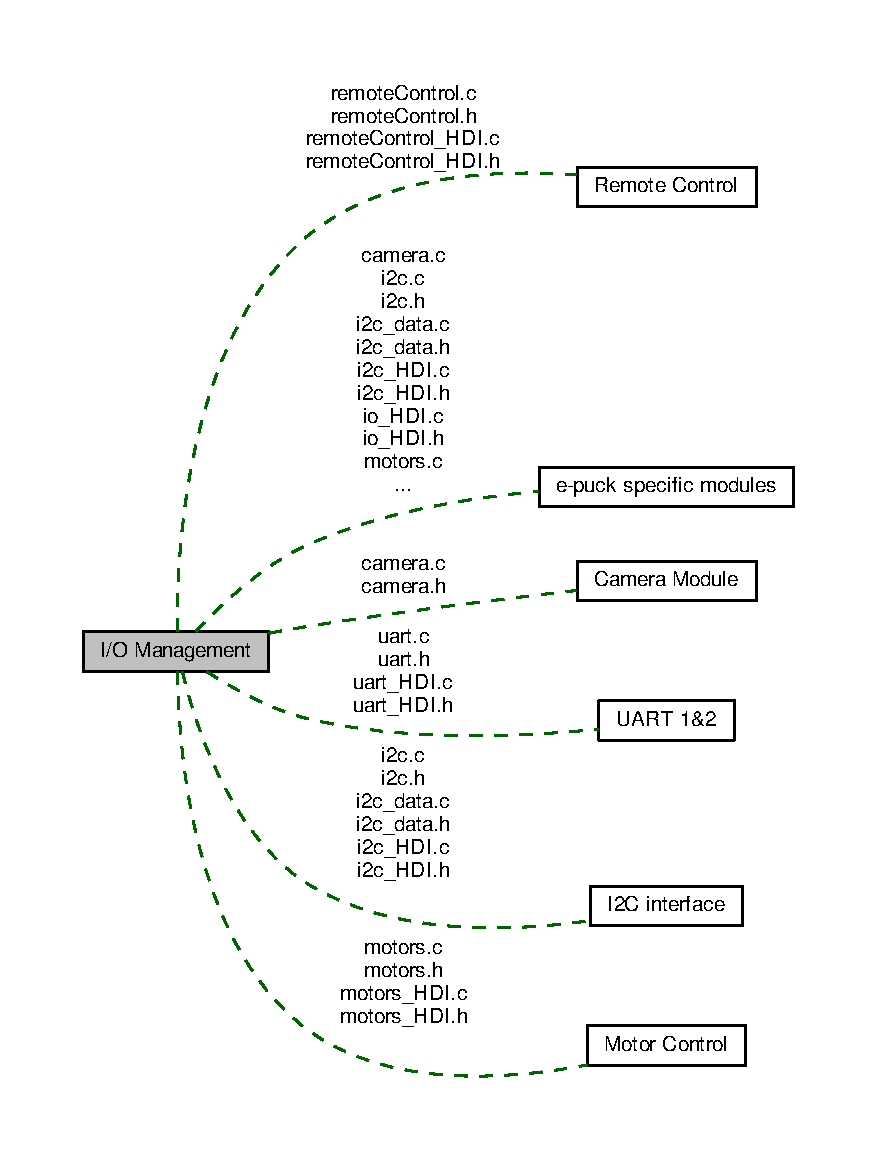
\includegraphics[width=350pt]{d2/da3/group__io}
\end{center}
\end{figure}
\subsection*{Files}
\begin{DoxyCompactItemize}
\item 
file \hyperlink{io_8c}{io.\+c}
\begin{DoxyCompactList}\small\item\em defines functions to control the I\+O timer and to (un)register I\+O Handler. \end{DoxyCompactList}\item 
file \hyperlink{io_8h}{io.\+h}
\begin{DoxyCompactList}\small\item\em declares functions to control the I\+O timer and to (un)register I\+O Handler. \end{DoxyCompactList}\item 
file \hyperlink{io__clock_8c}{io\+\_\+clock.\+c}
\begin{DoxyCompactList}\small\item\em defines the system clock that provides a continuous time value (granulation of 1 ms). \end{DoxyCompactList}\item 
file \hyperlink{io__clock_8h}{io\+\_\+clock.\+h}
\begin{DoxyCompactList}\small\item\em declares the system clock that provides a continuous time value (granulation of 1 ms). \end{DoxyCompactList}\item 
file \hyperlink{camera_8c}{camera.\+c}
\begin{DoxyCompactList}\small\item\em This file includes functions to process data retrieved by a camera. \end{DoxyCompactList}\item 
file \hyperlink{camera_8h}{camera.\+h}
\begin{DoxyCompactList}\small\item\em This file includes functions to process data retrieved by a camera. \end{DoxyCompactList}\item 
file \hyperlink{i2c_8c}{i2c.\+c}
\begin{DoxyCompactList}\small\item\em defines functions to read and write on the I2\+C interface. \end{DoxyCompactList}\item 
file \hyperlink{i2c_8h}{i2c.\+h}
\begin{DoxyCompactList}\small\item\em This file includes functions to read and write on the I2\+C interface. \end{DoxyCompactList}\item 
file \hyperlink{i2c__data_8c}{i2c\+\_\+data.\+c}
\begin{DoxyCompactList}\small\item\em defines functions to manage the I2\+C queue. \end{DoxyCompactList}\item 
file \hyperlink{i2c__data_8h}{i2c\+\_\+data.\+h}
\begin{DoxyCompactList}\small\item\em This file includes functions to read and write on the I2\+C interface. \end{DoxyCompactList}\item 
file \hyperlink{i2c__HDI_8c}{i2c\+\_\+\+H\+D\+I.\+c}
\begin{DoxyCompactList}\small\item\em Hardware dependent implementations to read and write on the I2\+C interface. \end{DoxyCompactList}\item 
file \hyperlink{i2c__HDI_8h}{i2c\+\_\+\+H\+D\+I.\+h}
\begin{DoxyCompactList}\small\item\em Hardware dependent implementations to read and write on the I2\+C interface. \end{DoxyCompactList}\item 
file \hyperlink{io__HDI_8c}{io\+\_\+\+H\+D\+I.\+c}
\begin{DoxyCompactList}\small\item\em Hardware dependent implementations to start and stop the I/\+O timer. This timer executes I\+O functions periodically. \end{DoxyCompactList}\item 
file \hyperlink{io__HDI_8h}{io\+\_\+\+H\+D\+I.\+h}
\begin{DoxyCompactList}\small\item\em Hardware dependent implementations to start and stop the I/\+O timer. This timer executes I\+O functions periodically. \end{DoxyCompactList}\item 
file \hyperlink{motors_8c}{motors.\+c}
\begin{DoxyCompactList}\small\item\em This file provides the function needed to actuate the motors. \end{DoxyCompactList}\item 
file \hyperlink{motors_8h}{motors.\+h}
\begin{DoxyCompactList}\small\item\em This file provides the function needed to actuate the motors. \end{DoxyCompactList}\item 
file \hyperlink{motors__HDI_8c}{motors\+\_\+\+H\+D\+I.\+c}
\begin{DoxyCompactList}\small\item\em Hardware dependent implementations to actuate the motors. \end{DoxyCompactList}\item 
file \hyperlink{motors__HDI_8h}{motors\+\_\+\+H\+D\+I.\+h}
\begin{DoxyCompactList}\small\item\em Hardware dependent implementations to actuate the motors. \end{DoxyCompactList}\item 
file \hyperlink{remoteControl_8c}{remote\+Control.\+c}
\begin{DoxyCompactList}\small\item\em This file includes functions needed to receive and decode messages from a remote control. \end{DoxyCompactList}\item 
file \hyperlink{remoteControl_8h}{remote\+Control.\+h}
\begin{DoxyCompactList}\small\item\em This file includes functions needed to receive and decode messages from a remote control. \end{DoxyCompactList}\item 
file \hyperlink{remoteControl__HDI_8c}{remote\+Control\+\_\+\+H\+D\+I.\+c}
\begin{DoxyCompactList}\small\item\em Hardware dependent implementations to receive and decode messages from a remote control. \end{DoxyCompactList}\item 
file \hyperlink{remoteControl__HDI_8h}{remote\+Control\+\_\+\+H\+D\+I.\+h}
\begin{DoxyCompactList}\small\item\em Hardware dependent implementations to receive and decode messages from a remote control. \end{DoxyCompactList}\item 
file \hyperlink{uart_8c}{uart.\+c}
\begin{DoxyCompactList}\small\item\em This file includes functions needed to transmit data via uart(1 \& 2). \end{DoxyCompactList}\item 
file \hyperlink{uart_8h}{uart.\+h}
\begin{DoxyCompactList}\small\item\em This file includes functions needed to transmit data via uart(1 \& 2). \end{DoxyCompactList}\item 
file \hyperlink{uart__HDI_8c}{uart\+\_\+\+H\+D\+I.\+c}
\begin{DoxyCompactList}\small\item\em Hardware dependent implementations to control the message flow of the U\+A\+R\+T interface. \end{DoxyCompactList}\item 
file \hyperlink{uart__HDI_8h}{uart\+\_\+\+H\+D\+I.\+h}
\begin{DoxyCompactList}\small\item\em Hardware dependent implementations to control the message flow of the U\+A\+R\+T interface. \end{DoxyCompactList}\end{DoxyCompactItemize}


\subsection{Detailed Description}
Functions and mechanisms to use I/\+O devices (e.\+g. sensors and actuators) to interact with the environment. 

\begin{DoxyAuthor}{Author}
Stefan M. Trenkwalder \href{mailto:s.trenkwalder@openswarm.org}{\tt s.\+trenkwalder@openswarm.\+org}
\end{DoxyAuthor}
\hypertarget{group__io_io_intro}{}\subsection{Introduction}\label{group__io_io_intro}
I/\+O device are managed by this module. I/\+O devices interfacing and interacting with the environment of the robot. These sensors and actuators might be a camera, motors, or gripper.

In general I/\+O devices might be independent and uses their own interrupts -\/ such as U\+A\+R\+T, A\+D\+C, I2\+C. These functions act independently and only need to be initialised and started. No further interaction is needed.

Many I/\+O devices however need periodic interactions -\/ such as remote control receiver, motor controller, or system clock.\hypertarget{group__io_io_usage}{}\subsection{Usage}\label{group__io_io_usage}
The I/\+O management is initialised with \hyperlink{io_8h_ad1719208a5855f34e056a8114de973f9}{Sys\+\_\+\+Init\+\_\+\+I\+O\+Management(void)}, which initialised the System Timer (100us) and initialises a list of I/\+O devices that need to be executed periodically. After starting the timer with \hyperlink{io_8h_a6ca66df90d159586d58a19e01f3a7025}{Sys\+\_\+\+Start\+\_\+\+I\+O\+Management(void)}, it can be the stopped with \hyperlink{io_8h_a14d9a8f941c03184049f3bf18d35fb47}{Sys\+\_\+\+Stop\+\_\+\+I\+O\+Management(void)}.

The I/\+O Timer can be manipulated as follows
\begin{DoxyItemize}
\item Stop\+: \hyperlink{io_8h_a3aa1e95e0e5be1866738b77f5b504652}{Sys\+\_\+\+Stop\+\_\+\+I\+O\+Timer(void)}
\item Continue\+: \hyperlink{io_8h_a15a4d1cf4ffaac43d2c1ae131652b869}{Sys\+\_\+\+Continue\+\_\+\+I\+O\+Timer(void)}
\item Reset (starts the 100us again)\+: \hyperlink{io_8h_a022c90f875bdb0b3cf2c85ab7872f531}{Sys\+\_\+\+Reset\+\_\+\+I\+O\+Timer(void)}
\item Disable\+: \hyperlink{io_8h_a21ac049cc8b67f8851decbbd0edf9dd6}{Sys\+\_\+\+Disable\+\_\+\+I\+O\+Timer\+Interrupt(void)}
\item Enable\+: \hyperlink{io_8h_aefef1e8eb442327a4b4c7bc89d6d13ce}{Sys\+\_\+\+Enable\+\_\+\+I\+O\+Timer\+Interrupt(void)}
\item Force an I/\+O Timer interrupt\+: \hyperlink{io_8h_ac23e12fcd2478b2d820aa55dcd9460ee}{Sys\+\_\+\+Force\+\_\+\+I\+O\+Timer\+Interrupt(void)}
\end{DoxyItemize}

New I/\+O devices can be added and removed by (un)registering with \hyperlink{io_8h_a915425274eaebb4ed39d8622b90993b7}{Sys\+\_\+\+Register\+\_\+\+I\+O\+Handler(p\+Function func)} and \hyperlink{io_8h_a1b695aa5cbdf06b543b10b9661722d36}{Sys\+\_\+\+Unregister\+\_\+\+I\+O\+Handler(p\+Function func)}.

The I/\+O management is started by initialising \& starting of the kernel \begin{DoxySeeAlso}{See also}
\hyperlink{group__base}{Base}
\end{DoxySeeAlso}
\hypertarget{group__io_io_license}{}\subsection{License}\label{group__io_io_license}
L\+I\+C\+E\+N\+S\+E\+: adapted Free\+B\+S\+D License (see \href{http://openswarm.org/license}{\tt http\+://openswarm.\+org/license})~\newline
Copyright (c) 2015, Stefan M. Trenkwalder~\newline
All rights reserved. 
\hypertarget{group__camera}{}\section{Camera Module}
\label{group__camera}\index{Camera Module@{Camera Module}}


Functions to process incoming frames from a camera module.  


Collaboration diagram for Camera Module\+:\nopagebreak
\begin{figure}[H]
\begin{center}
\leavevmode
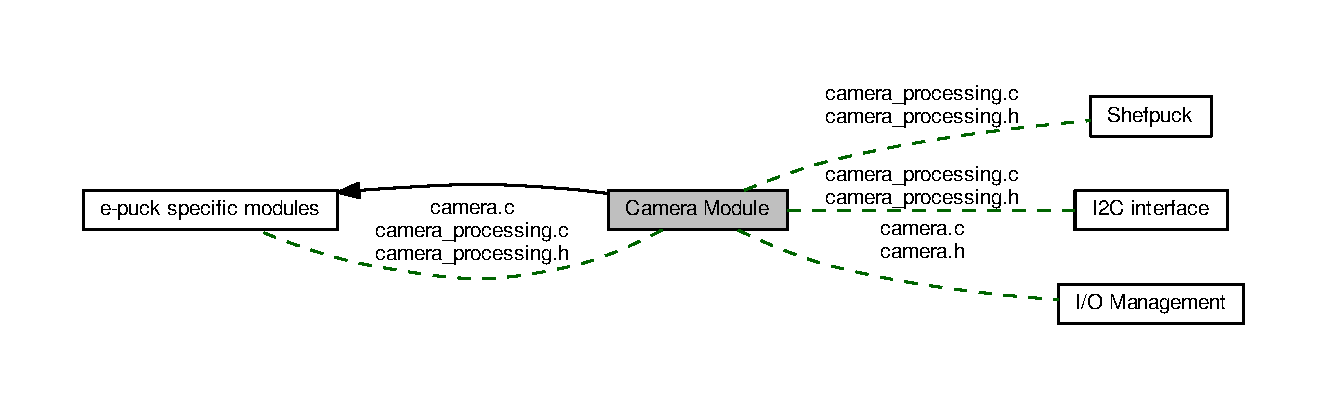
\includegraphics[width=350pt]{dc/d90/group__camera}
\end{center}
\end{figure}
\subsection*{Files}
\begin{DoxyCompactItemize}
\item 
file \hyperlink{camera_8c}{camera.\+c}
\begin{DoxyCompactList}\small\item\em This file includes functions to process data retrieved by a camera. \end{DoxyCompactList}\item 
file \hyperlink{camera_8h}{camera.\+h}
\begin{DoxyCompactList}\small\item\em This file includes functions to process data retrieved by a camera. \end{DoxyCompactList}\item 
file \hyperlink{camera__processing_8c}{camera\+\_\+processing.\+c}
\item 
file \hyperlink{camera__processing_8h}{camera\+\_\+processing.\+h}
\end{DoxyCompactItemize}


\subsection{Detailed Description}
Functions to process incoming frames from a camera module. 

\begin{DoxyAuthor}{Author}
Stefan M. Trenkwalder \href{mailto:s.trenkwalder@openswarm.org}{\tt s.\+trenkwalder@openswarm.\+org}
\end{DoxyAuthor}
\hypertarget{group__camera_camera_intro}{}\subsection{Introduction}\label{group__camera_camera_intro}
This module is part of the I/\+O handler. \begin{DoxySeeAlso}{See also}
\hyperlink{group__io}{I/\+O Management}
\end{DoxySeeAlso}
This module currently is under development and is using functions of the e-\/puck library provided using Subversion at svn\+://svn.gna.\+org/svn/e-\/puck/trunk .

\begin{DoxyRefDesc}{Todo}
\item[\hyperlink{todo__todo000005}{Todo}]The used functions from the e-\/puck library are very time and computational intensive. These function can be rewritten to decrease the processing load.\end{DoxyRefDesc}
\hypertarget{group__camera_camera_usage}{}\subsection{Usage}\label{group__camera_camera_usage}
The camera is initialised and started by Sys\+\_\+\+Init\+\_\+\+Camera and Sys\+\_\+\+Start\+\_\+\+Camera respectively.

The camera uses a preprocessor to process a frame and generate the required events. This preprocessor can be defined by \hyperlink{camera_8h_ac93ec56d124a0811e638208ad64ed14c}{Sys\+\_\+\+Set\+\_\+\+Preprocessing(p\+Camera\+Pre\+Processor)}.

A received frame, if available (\hyperlink{camera_8h_a1b0543ca3f9389e59135838a3c9cbb23}{is\+New\+Frame\+Available()}) can be obtained with \hyperlink{camera_8h_a72c1d6c27d3aeb8399ec41247cc4ba58}{get\+Finished\+Frame()}.\hypertarget{group__camera_camera_license}{}\subsection{License}\label{group__camera_camera_license}
L\+I\+C\+E\+N\+S\+E\+: adapted Free\+B\+S\+D License (see \href{http://openswarm.org/license}{\tt http\+://openswarm.\+org/license})~\newline
Copyright (c) 2015, Stefan M. Trenkwalder~\newline
All rights reserved. 
\hypertarget{group__shefpuck}{}\subsection{Shefpuck}
\label{group__shefpuck}\index{Shefpuck@{Shefpuck}}


External set of functions to assist the programming of the e-\/\+Puck.  


Collaboration diagram for Shefpuck\+:\nopagebreak
\begin{figure}[H]
\begin{center}
\leavevmode
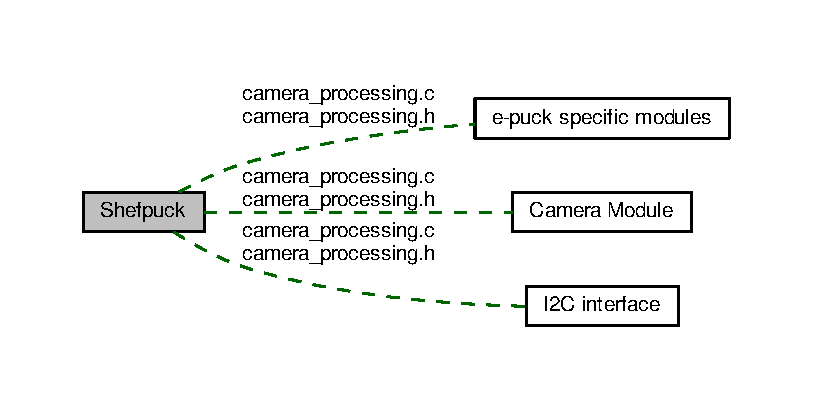
\includegraphics[width=350pt]{d9/d96/group__shefpuck}
\end{center}
\end{figure}
\subsubsection*{Files}
\begin{DoxyCompactItemize}
\item 
file \hyperlink{camera__processing_8c}{camera\+\_\+processing.\+c}
\item 
file \hyperlink{camera__processing_8h}{camera\+\_\+processing.\+h}
\begin{DoxyCompactList}\small\item\em External set of functions to assist the use of the camera. (provided by \hyperlink{group__shefpuck}{Shefpuck} ) \end{DoxyCompactList}\end{DoxyCompactItemize}


\subsubsection{Detailed Description}
External set of functions to assist the programming of the e-\/\+Puck. 

\begin{DoxyAuthor}{Author}
Yuri Kaszubowski Lopes \href{mailto:yurikazuba@gmail.com}{\tt yurikazuba@gmail.\+com}
\end{DoxyAuthor}
This file is part of shefpuck.

This library is in development.\hypertarget{group__shefpuck_License}{}\subsubsection{License}\label{group__shefpuck_License}
shefpuck is free software\+: you can redistribute it and/or modify it under the terms of the G\+N\+U Lesser General Public License as published by the Free Software Foundation, either version 3 of the License, or (at your option) any later version.

shefpuck is distributed in the hope that it will be useful, but W\+I\+T\+H\+O\+U\+T A\+N\+Y W\+A\+R\+R\+A\+N\+T\+Y; without even the implied warranty of M\+E\+R\+C\+H\+A\+N\+T\+A\+B\+I\+L\+I\+T\+Y or F\+I\+T\+N\+E\+S\+S F\+O\+R A P\+A\+R\+T\+I\+C\+U\+L\+A\+R P\+U\+R\+P\+O\+S\+E. See the G\+N\+U Lesser General Public License for more details.

You should have received a copy of the G\+N\+U Lesser General Public License along with shefpuck. If not, see \href{http://www.gnu.org/licenses/}{\tt http\+://www.\+gnu.\+org/licenses/}. Copyright (C) 2014-\/2015 Yuri Kaszubowski Lopes -\/ \href{mailto:yurikazuba@gmail.com}{\tt yurikazuba@gmail.\+com}

\begin{DoxyNote}{Note}
Due to the use of the e-\/puck library while processing the camera input, this module is used to process a camera frame into a virtual simple line of sight sensor value. This module, as well as the functions used from the e-\/puck library, will be replaced. 
\end{DoxyNote}

\hypertarget{group__epuck}{}\subsection{e-\/puck specific modules}
\label{group__epuck}\index{e-\/puck specific modules@{e-\/puck specific modules}}


Modules and functions that are needed to use the e-\/puck platform ( \href{http://www.gctronic.com/doc/index.php/E-Puck}{\tt http\+://www.\+gctronic.\+com/doc/index.\+php/\+E-\/\+Puck} )  


Collaboration diagram for e-\/puck specific modules\+:\nopagebreak
\begin{figure}[H]
\begin{center}
\leavevmode
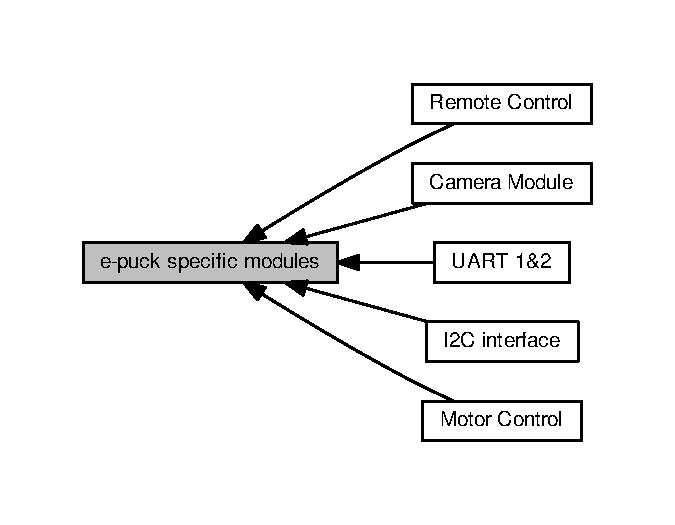
\includegraphics[width=324pt]{d9/dc8/group__epuck}
\end{center}
\end{figure}
\subsubsection*{Modules}
\begin{DoxyCompactItemize}
\item 
\hyperlink{group__camera}{Camera Module}
\begin{DoxyCompactList}\small\item\em The camera module is used to retrieve raw camera data, process the incoming frames, and emits the result as \hyperlink{group__events}{events}. \end{DoxyCompactList}\item 
\hyperlink{group__i2c}{I2\+C interface}
\begin{DoxyCompactList}\small\item\em Functions to read from and write on the I2\+C interface. \end{DoxyCompactList}\item 
\hyperlink{group__motors}{Motor Control}
\begin{DoxyCompactList}\small\item\em Functions to control the two stepper motors of the e-\/puck. \end{DoxyCompactList}\item 
\hyperlink{group__remotecontrol}{Remote Control}
\begin{DoxyCompactList}\small\item\em Functions to receive data from a remote control. \end{DoxyCompactList}\item 
\hyperlink{group__uart}{U\+A\+R\+T 1\&2}
\begin{DoxyCompactList}\small\item\em Functions to control the message flow of the U\+A\+R\+T interface. \end{DoxyCompactList}\end{DoxyCompactItemize}
\subsubsection*{Files}
\begin{DoxyCompactItemize}
\item 
file \hyperlink{DSPIC30F6014A__HDI_8h}{D\+S\+P\+I\+C30\+F6014\+A\+\_\+\+H\+D\+I.\+h}
\begin{DoxyCompactList}\small\item\em declares e-\/puck specific types and preprocessor variables \end{DoxyCompactList}\item 
file \hyperlink{traps_8c}{traps.\+c}
\begin{DoxyCompactList}\small\item\em Hardware dependent implementations to catch hardware traps. \end{DoxyCompactList}\end{DoxyCompactItemize}


\subsubsection{Detailed Description}
Modules and functions that are needed to use the e-\/puck platform ( \href{http://www.gctronic.com/doc/index.php/E-Puck}{\tt http\+://www.\+gctronic.\+com/doc/index.\+php/\+E-\/\+Puck} ) 

\begin{DoxyAuthor}{Author}
Stefan M. Trenkwalder \href{mailto:s.trenkwalder@openswarm.org}{\tt s.\+trenkwalder@openswarm.\+org}
\end{DoxyAuthor}
\hypertarget{group__epuck_Provided}{}\subsubsection{Features}\label{group__epuck_Provided}
The e-\/puck provides the following features\+: \hypertarget{group__epuck_epuck_sensor}{}\paragraph{Sensors\+:}\label{group__epuck_epuck_sensor}
\hypertarget{group__epuck_epuck_prox}{}\subparagraph{8 infra-\/red proximity sensors}\label{group__epuck_epuck_prox}
The infra-\/red proximity sensors are currently under implementation. Therefore not ready yet. \hypertarget{group__epuck_epuck_acc}{}\subparagraph{accelerometer}\label{group__epuck_epuck_acc}
The accelerometer weren\textquotesingle{}t needed for many applications and, therefore, the priority to implement the accelerometer is small. \hypertarget{group__epuck_epuck_mic}{}\subparagraph{3 microphones}\label{group__epuck_epuck_mic}
The microphones weren\textquotesingle{}t needed for many applications and, therefore, the priority to implement the microphones is small. \hypertarget{group__epuck_epuck_camera}{}\subparagraph{camera\+:}\label{group__epuck_epuck_camera}
The camera functions can be found at \hyperlink{group__camera}{Camera Module} \hypertarget{group__epuck_epuck_remote}{}\subparagraph{remote control receiver\+:}\label{group__epuck_epuck_remote}
This function is fully implemented (\hyperlink{group__remotecontrol}{Remote Control} ). \hypertarget{group__epuck_epuck_output}{}\paragraph{Actuators\+:}\label{group__epuck_epuck_output}
\hypertarget{group__epuck_epuck_motors}{}\subparagraph{differential drive (\textbackslash{}ref motors ).}\label{group__epuck_epuck_motors}
\hypertarget{group__epuck_epuck_led}{}\subparagraph{leds\+:}\label{group__epuck_epuck_led}
Hardware independent functions to control the L\+E\+Ds are not yet implemented, due to it\textquotesingle{}s simple nature. Currently you can use the M\+A\+C\+R\+Os L\+E\+D0, L\+E\+D1, ..., L\+E\+D7, B\+O\+D\+Y\+L\+E\+D, F\+R\+O\+N\+T\+L\+E\+D to set and unset these L\+E\+Ds. \hypertarget{group__epuck_epuck_speaker}{}\subparagraph{speaker\+:}\label{group__epuck_epuck_speaker}
The speakers weren\textquotesingle{}t needed for many applications and, therefore, the priority to implement the speakers is small. \hypertarget{group__epuck_epuck_com}{}\paragraph{communication\+:}\label{group__epuck_epuck_com}
\hypertarget{group__epuck_epuck_bluetooth}{}\subparagraph{Bluetooth\+:}\label{group__epuck_epuck_bluetooth}
The Bluetooth can be used by sending and receiving bytes via U\+A\+R\+T1 (\hyperlink{group__uart}{U\+A\+R\+T 1\&2} ) \hypertarget{group__epuck_epuck_ircom}{}\subparagraph{Infra-\/red communication}\label{group__epuck_epuck_ircom}
The infra-\/red proximity sensors can be used to transmit and receive data. This function leads to a local broadcasting. However, this function is still under development.\hypertarget{group__epuck_epuck_license}{}\subsubsection{License}\label{group__epuck_epuck_license}
L\+I\+C\+E\+N\+S\+E\+: adapted Free\+B\+S\+D License (see \href{http://openswarm.org/license}{\tt http\+://openswarm.\+org/license})~\newline
Copyright (c) 2015, Stefan M. Trenkwalder~\newline
All rights reserved. 
\hypertarget{group__i2c}{}\subsection{I2\+C interface}
\label{group__i2c}\index{I2\+C interface@{I2\+C interface}}


Functions to read from and write on the I2\+C interface.  


Collaboration diagram for I2\+C interface\+:\nopagebreak
\begin{figure}[H]
\begin{center}
\leavevmode
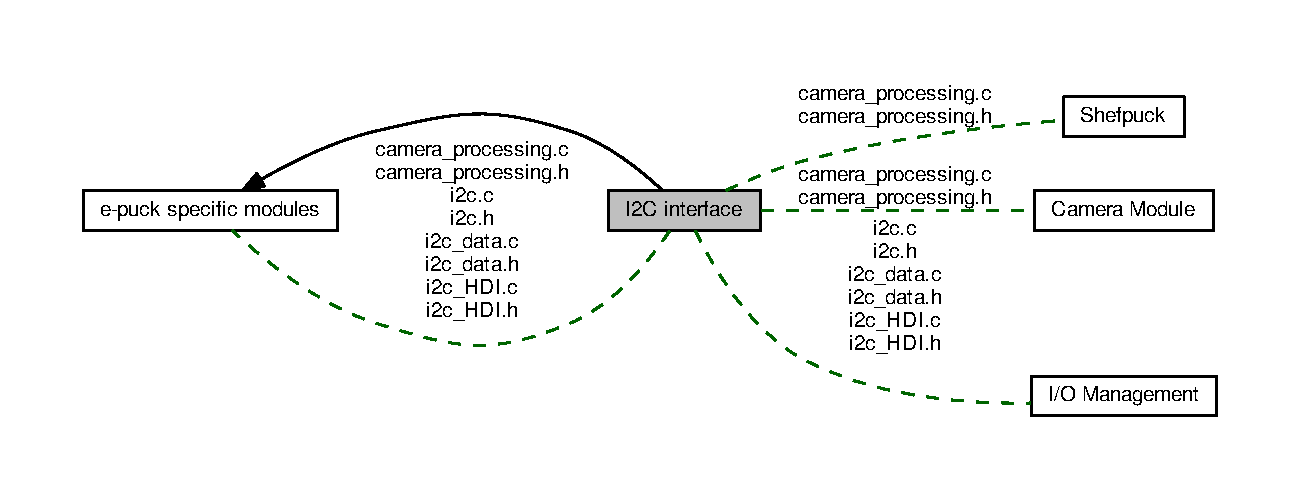
\includegraphics[width=311pt]{d3/df5/group__i2c}
\end{center}
\end{figure}
\subsubsection*{Files}
\begin{DoxyCompactItemize}
\item 
file \hyperlink{i2c_8c}{i2c.\+c}
\begin{DoxyCompactList}\small\item\em It defines functions to read and write on the I2\+C interface. \end{DoxyCompactList}\item 
file \hyperlink{i2c_8h}{i2c.\+h}
\begin{DoxyCompactList}\small\item\em It declares functions to read and write on the I2\+C interface. \end{DoxyCompactList}\item 
file \hyperlink{i2c__data_8c}{i2c\+\_\+data.\+c}
\begin{DoxyCompactList}\small\item\em It defines functions to manage the I2\+C queue. \end{DoxyCompactList}\item 
file \hyperlink{i2c__data_8h}{i2c\+\_\+data.\+h}
\begin{DoxyCompactList}\small\item\em It declares functions to manage the I2\+C queue. \end{DoxyCompactList}\item 
file \hyperlink{i2c__HDI_8c}{i2c\+\_\+\+H\+D\+I.\+c}
\begin{DoxyCompactList}\small\item\em Hardware dependent implementations to read and write on the I2\+C interface. \end{DoxyCompactList}\item 
file \hyperlink{i2c__HDI_8h}{i2c\+\_\+\+H\+D\+I.\+h}
\begin{DoxyCompactList}\small\item\em Hardware dependent implementations to read and write on the I2\+C interface. \end{DoxyCompactList}\end{DoxyCompactItemize}


\subsubsection{Detailed Description}
Functions to read from and write on the I2\+C interface. 

\begin{DoxyAuthor}{Author}
Stefan M. Trenkwalder \href{mailto:s.trenkwalder@openswarm.org}{\tt s.\+trenkwalder@openswarm.\+org}
\end{DoxyAuthor}
Inter-\/\+Integrated Circuit bus is a multi-\/master, multi-\/slave, serial bus (see also \href{https://en.wikipedia.org/wiki/I%C2%B2C}{\tt https\+://en.\+wikipedia.\+org/wiki/\+I\%\+C2\%\+B2\+C} )\hypertarget{group__i2c_i2c_usage}{}\subsubsection{Usage}\label{group__i2c_i2c_usage}
The I2\+C interface can be initialised and started with \hyperlink{i2c_8h_ae0e15cb80a0603c250857c1a799a62f5}{Sys\+\_\+\+Init\+\_\+\+I2\+C()} and \hyperlink{i2c_8h_a47a8891b8d4ec015d28d2fb38db7af81}{Sys\+\_\+\+Start\+\_\+\+I2\+C()} respectively. Similarly, it can be paused, continued, or stopped by \hyperlink{i2c_8h_a5093f0861938b0821984309c08ed245a}{Sys\+\_\+\+Pause\+\_\+\+I2\+C()}, \hyperlink{i2c_8h_afd7fe98d1cae4221b8541e2f232a1fe8}{Sys\+\_\+\+Contine\+\_\+\+I2\+C()}, or \hyperlink{i2c_8h_a808f963da209bf3a2437be9ac98b3ae3}{Sys\+\_\+\+Stop\+\_\+\+I2\+C()} respectively. While the interface is running, data can be written with \hyperlink{i2c_8h_aae28d108698f25ca0465e1b57d28eaaa}{Sys\+\_\+\+I2\+C\+\_\+\+Sent\+Bytes(uint8, uint8 $\ast$, uint16)}. Values can be read with \hyperlink{i2c_8h_ac368d180152e0f85b5b5f210ad7dc573}{Sys\+\_\+\+I2\+C\+\_\+\+Read(uint8 , uint8 $\ast$, uint16, p\+Byte\+Function)} where the request message has also to be specified.

\begin{DoxyRefDesc}{Todo}
\item[\hyperlink{todo__todo000006}{Todo}]testing and debugging of this module.\end{DoxyRefDesc}


\begin{DoxyNote}{Note}
This module is currently untested. It might not work or includes some bugs. The interrupt handler \+\_\+\+M\+I2\+C\+Interrupt() is also out commented, because it might interfere with the e-\/\+Puck library used in the camera module.
\end{DoxyNote}
\hypertarget{group__i2c_i2c_license}{}\subsubsection{License}\label{group__i2c_i2c_license}
L\+I\+C\+E\+N\+S\+E\+: adapted Free\+B\+S\+D License (see \href{http://openswarm.org/license}{\tt http\+://openswarm.\+org/license})~\newline
Copyright (c) 2015, Stefan M. Trenkwalder~\newline
All rights reserved. 
\hypertarget{group__motors}{}\section{Motor Control}
\label{group__motors}\index{Motor Control@{Motor Control}}


Functions to control the motors.  


Collaboration diagram for Motor Control\+:\nopagebreak
\begin{figure}[H]
\begin{center}
\leavevmode
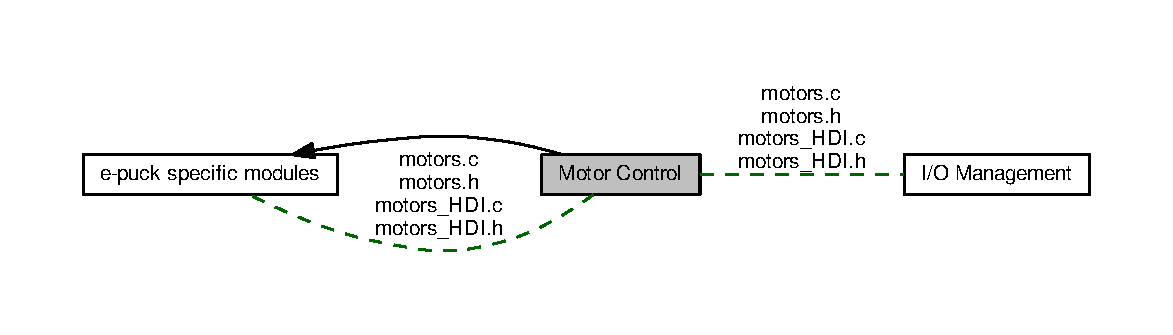
\includegraphics[width=350pt]{dd/daa/group__motors}
\end{center}
\end{figure}
\subsection*{Files}
\begin{DoxyCompactItemize}
\item 
file \hyperlink{motors_8c}{motors.\+c}
\begin{DoxyCompactList}\small\item\em This file provides the function needed to actuate the motors. \end{DoxyCompactList}\item 
file \hyperlink{motors_8h}{motors.\+h}
\begin{DoxyCompactList}\small\item\em This file provides the function needed to actuate the motors. \end{DoxyCompactList}\item 
file \hyperlink{motors__HDI_8c}{motors\+\_\+\+H\+D\+I.\+c}
\begin{DoxyCompactList}\small\item\em Hardware dependent implementations to actuate the motors. \end{DoxyCompactList}\item 
file \hyperlink{motors__HDI_8h}{motors\+\_\+\+H\+D\+I.\+h}
\begin{DoxyCompactList}\small\item\em Hardware dependent implementations to actuate the motors. \end{DoxyCompactList}\end{DoxyCompactItemize}


\subsection{Detailed Description}
Functions to control the motors. 

\begin{DoxyAuthor}{Author}
Stefan M. Trenkwalder \href{mailto:s.trenkwalder@openswarm.org}{\tt s.\+trenkwalder@openswarm.\+org}
\end{DoxyAuthor}
The motor control module controls the speed and motion of motors\hypertarget{group__motors_motors_usage}{}\subsection{Usage}\label{group__motors_motors_usage}
After the initialisation with \hyperlink{motors_8h_ab35833b8a72da88c16285b4ff4d24eb5}{Sys\+\_\+\+Init\+\_\+\+Motors()}, the motors can be used by setting the motor speed. This can be done by sending the motor velocities via events to S\+Y\+S\+\_\+\+E\+V\+E\+N\+T\+\_\+\+I\+O\+\_\+\+M\+O\+T\+O\+R\+\_\+\+L\+E\+F\+T and S\+Y\+S\+\_\+\+E\+V\+E\+N\+T\+\_\+\+I\+O\+\_\+\+M\+O\+T\+O\+R\+\_\+\+R\+I\+G\+H\+T or by setting the speed directly by calling \hyperlink{motors_8h_a3bd56e9540443f08d15bdef558e77dd5}{Sys\+\_\+\+Set\+\_\+\+Left\+Wheel\+Speed(sint16)} and \hyperlink{motors_8h_a497d00bbd91ce1308c6e6d15d16b482d}{Sys\+\_\+\+Set\+\_\+\+Right\+Wheel\+Speed(sint16)}. The current speed can be obtained Sys\+\_\+get\+\_\+\+Left\+Wheel\+Speed() and Sys\+\_\+get\+\_\+\+Right\+Wheel\+Speed().\hypertarget{group__motors_motors_license}{}\subsection{License}\label{group__motors_motors_license}
L\+I\+C\+E\+N\+S\+E\+: adapted Free\+B\+S\+D License (see \href{http://openswarm.org/license}{\tt http\+://openswarm.\+org/license})~\newline
Copyright (c) 2015, Stefan M. Trenkwalder~\newline
All rights reserved. 
\hypertarget{group__remotecontrol}{}\section{Remote Control}
\label{group__remotecontrol}\index{Remote Control@{Remote Control}}


Functions to receive data from a remote control.  


Collaboration diagram for Remote Control\+:\nopagebreak
\begin{figure}[H]
\begin{center}
\leavevmode
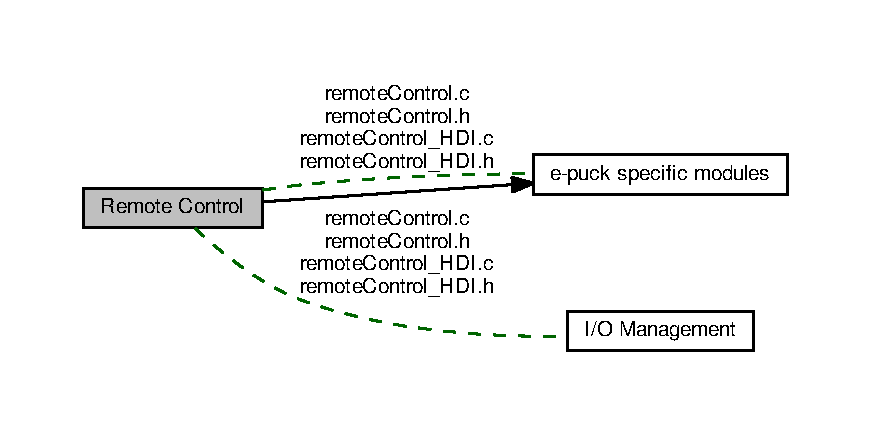
\includegraphics[width=350pt]{db/d36/group__remotecontrol}
\end{center}
\end{figure}
\subsection*{Files}
\begin{DoxyCompactItemize}
\item 
file \hyperlink{remoteControl_8c}{remote\+Control.\+c}
\begin{DoxyCompactList}\small\item\em This file includes functions needed to receive and decode messages from a remote control. \end{DoxyCompactList}\item 
file \hyperlink{remoteControl_8h}{remote\+Control.\+h}
\begin{DoxyCompactList}\small\item\em This file includes functions needed to receive and decode messages from a remote control. \end{DoxyCompactList}\item 
file \hyperlink{remoteControl__HDI_8c}{remote\+Control\+\_\+\+H\+D\+I.\+c}
\begin{DoxyCompactList}\small\item\em Hardware dependent implementations to receive and decode messages from a remote control. \end{DoxyCompactList}\item 
file \hyperlink{remoteControl__HDI_8h}{remote\+Control\+\_\+\+H\+D\+I.\+h}
\begin{DoxyCompactList}\small\item\em Hardware dependent implementations to receive and decode messages from a remote control. \end{DoxyCompactList}\end{DoxyCompactItemize}


\subsection{Detailed Description}
Functions to receive data from a remote control. 

\begin{DoxyAuthor}{Author}
Stefan M. Trenkwalder \href{mailto:s.trenkwalder@openswarm.org}{\tt s.\+trenkwalder@openswarm.\+org}
\end{DoxyAuthor}
This module is based on the R\+C-\/5 coding for the (Toshiba R\+C-\/3910)\hypertarget{group__remotecontrol_rc_usage}{}\subsection{Usage}\label{group__remotecontrol_rc_usage}
After the initialisation with \hyperlink{remoteControl_8h_a3265e493859892f6ebca8df6252d6f8e}{Sys\+\_\+\+Init\+\_\+\+Remote\+Control()}, the interface needs to be started to be able to receive or transmit bytes with \hyperlink{remoteControl_8h_a5aaecc26aad6d1c545a225b1ce92cec7}{Sys\+\_\+\+Start\+\_\+\+Remote\+Control()}.

After this every button pressed on the remote control is received as an event (S\+Y\+S\+\_\+\+E\+V\+E\+N\+T\+\_\+\+I\+O\+\_\+\+R\+E\+M\+O\+E\+C\+O\+N\+T\+R\+O\+L).\hypertarget{group__remotecontrol_rc_license}{}\subsection{License}\label{group__remotecontrol_rc_license}
L\+I\+C\+E\+N\+S\+E\+: adapted Free\+B\+S\+D License (see \href{http://openswarm.org/license}{\tt http\+://openswarm.\+org/license})~\newline
Copyright (c) 2015, Stefan M. Trenkwalder~\newline
All rights reserved. 
\hypertarget{group__uart}{}\section{U\+A\+R\+T 1\&2}
\label{group__uart}\index{U\+A\+R\+T 1\&2@{U\+A\+R\+T 1\&2}}


Functions to control the message flow of the U\+A\+R\+T interface.  


Collaboration diagram for U\+A\+R\+T 1\&2\+:\nopagebreak
\begin{figure}[H]
\begin{center}
\leavevmode
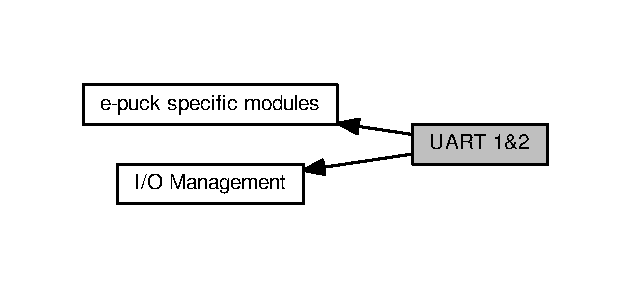
\includegraphics[width=350pt]{db/def/group__uart}
\end{center}
\end{figure}
\subsection*{Files}
\begin{DoxyCompactItemize}
\item 
file \hyperlink{uart_8c}{uart.\+c}
\begin{DoxyCompactList}\small\item\em This file includes functions needed to transmit data via uart(1 \& 2). \end{DoxyCompactList}\item 
file \hyperlink{uart_8h}{uart.\+h}
\begin{DoxyCompactList}\small\item\em This file includes functions needed to transmit data via uart(1 \& 2). \end{DoxyCompactList}\item 
file \hyperlink{uart__HDI_8c}{uart\+\_\+\+H\+D\+I.\+c}
\begin{DoxyCompactList}\small\item\em Hardware dependent implementations to control the message flow of the U\+A\+R\+T interface. \end{DoxyCompactList}\item 
file \hyperlink{uart__HDI_8h}{uart\+\_\+\+H\+D\+I.\+h}
\begin{DoxyCompactList}\small\item\em Hardware dependent implementations to control the message flow of the U\+A\+R\+T interface. \end{DoxyCompactList}\end{DoxyCompactItemize}


\subsection{Detailed Description}
Functions to control the message flow of the U\+A\+R\+T interface. 

\begin{DoxyAuthor}{Author}
Stefan M. Trenkwalder \href{mailto:s.trenkwalder@openswarm.org}{\tt s.\+trenkwalder@openswarm.\+org}
\end{DoxyAuthor}
A U\+A\+R\+T (Universal Asynchronous Receiver Transmitter) interface is common on microcontroller to communicate with other devices on a serial bus. \begin{DoxySeeAlso}{See also}
\href{https://en.wikipedia.org/wiki/Universal_asynchronous_receiver/transmitter}{\tt https\+://en.\+wikipedia.\+org/wiki/\+Universal\+\_\+asynchronous\+\_\+receiver/transmitter} The U\+A\+R\+T 1 is used on the \hyperlink{group__epuck}{e-\/puck specific modules} to communicate with the Bluetooth transceiver.
\end{DoxySeeAlso}
\hypertarget{group__uart_uart_usage}{}\subsection{Usage}\label{group__uart_uart_usage}
After the initialisation with \hyperlink{uart_8h_a64689486ee92e3dcd519778bc7afd3de}{Sys\+\_\+\+Init\+\_\+\+U\+A\+R\+T1()} (same applies to U\+A\+R\+T2), the U\+A\+R\+T interface needs to be started to be able to receive or transmit bytes. This can be done by sending the bytes via event to S\+Y\+S\+\_\+\+E\+V\+E\+N\+T\+\_\+\+I\+O\+\_\+\+T\+O\+\_\+\+B\+L\+U\+E\+T\+O\+O\+T\+H (U\+A\+R\+T1) or by handing over the bytes directly by calling Sys\+\_\+\+Writeto\+\_\+\+U\+A\+R\+T1 and Sys\+\_\+\+Writeto\+\_\+\+U\+A\+R\+T2. Incoming bytes can be received by defining a reading function with \hyperlink{uart_8h_a09b6e9f0a90b382e5bb453035ca337af}{Sys\+\_\+\+Set\+Reading\+Function\+\_\+\+U\+A\+R\+T1(p\+U\+A\+R\+T\+\_\+reader)} and \hyperlink{uart_8h_a9fad382ce87c7296fe5ba2005d0a7b10}{Sys\+\_\+\+Set\+Reading\+Function\+\_\+\+U\+A\+R\+T2(p\+U\+A\+R\+T\+\_\+reader)}. This function is executed every time a new byte arrives.\hypertarget{group__uart_uart_license}{}\subsection{License}\label{group__uart_uart_license}
L\+I\+C\+E\+N\+S\+E\+: adapted Free\+B\+S\+D License (see \href{http://openswarm.org/license}{\tt http\+://openswarm.\+org/license})~\newline
Copyright (c) 2015, Stefan M. Trenkwalder~\newline
All rights reserved. 
\hypertarget{group__process}{}\section{Process Manages}
\label{group__process}\index{Process Manages@{Process Manages}}


Functions to create, switch, block, yield, and terminate processes and start critical sections.  


\subsection*{Files}
\begin{DoxyCompactItemize}
\item 
file \hyperlink{process__Management__HDI_8c}{process\+\_\+\+Management\+\_\+\+H\+D\+I.\+c}
\begin{DoxyCompactList}\small\item\em Hardware dependent implementations to manage processes (e.\+g. task swichting) \end{DoxyCompactList}\item 
file \hyperlink{process__Management__HDI_8h}{process\+\_\+\+Management\+\_\+\+H\+D\+I.\+h}
\begin{DoxyCompactList}\small\item\em Hardware dependent implementations to manage processes (e.\+g. task swichting) \end{DoxyCompactList}\item 
file \hyperlink{data_8c}{data.\+c}
\begin{DoxyCompactList}\small\item\em This file includes all functions which are needed to manage data structures needed by the processes management. \end{DoxyCompactList}\item 
file \hyperlink{data_8h}{data.\+h}
\begin{DoxyCompactList}\small\item\em This file includes all functions which are needed to manage data structures needed by the processes management. \end{DoxyCompactList}\item 
file \hyperlink{process__Management_8c}{process\+\_\+\+Management.\+c}
\begin{DoxyCompactList}\small\item\em This file includes all functions wich are needed to manage processes (e.\+g. task swichting) \end{DoxyCompactList}\item 
file \hyperlink{process__Management_8h}{process\+\_\+\+Management.\+h}
\begin{DoxyCompactList}\small\item\em This file includes all functions wich are needed to manage processes (e.\+g. task creation, switching, termination) \end{DoxyCompactList}\item 
file \hyperlink{scheduler_8c}{scheduler.\+c}
\begin{DoxyCompactList}\small\item\em This file includes all functions wich are needed to specify a scheduling algorithm. \end{DoxyCompactList}\item 
file \hyperlink{scheduler_8h}{scheduler.\+h}
\begin{DoxyCompactList}\small\item\em This file includes all functions wich are needed to specify a scheduling algorithm. \end{DoxyCompactList}\item 
file \hyperlink{system__Timer_8c}{system\+\_\+\+Timer.\+c}
\begin{DoxyCompactList}\small\item\em This file includes all hardware dependent functions, which are nesessary to initialise, configure and run the system Time. \end{DoxyCompactList}\item 
file \hyperlink{system__Timer_8h}{system\+\_\+\+Timer.\+h}
\begin{DoxyCompactList}\small\item\em This file includes all hardware dependent functions, which are nesessary to initialise, configure and run the system Time. \end{DoxyCompactList}\end{DoxyCompactItemize}


\subsection{Detailed Description}
Functions to create, switch, block, yield, and terminate processes and start critical sections. 

\begin{DoxyAuthor}{Author}
Stefan M. Trenkwalder \href{mailto:s.trenkwalder@openswarm.org}{\tt s.\+trenkwalder@openswarm.\+org}
\end{DoxyAuthor}
A process is a basic form to execute functions in Open\+Swarm. Open\+Swarm does not provide functions to separate memory in pages or segments due to target device architecture. Because all processes are executed in the same memory area, each process can be seen as a single thread and all threads share the same memory. A thread is just represented by a common function. One function can be executed multiple times as individual threads.

Open\+Swarm organises processes in three lists of processes (pid sorted)\+:
\begin{DoxyEnumerate}
\item running list\+: includes all processes are ready to be executed and are scheduled according to the scheduling algorithm.
\item blocked list\+: includes all processes that are waiting for events to occur.
\item Zombie list\+: includes all processes that are about to be terminated but not deleted yet.
\end{DoxyEnumerate}\hypertarget{group__process_process_usage}{}\subsection{Usage}\label{group__process_process_usage}
The process management is initialised with \hyperlink{process__Management_8h_ae2b7783ff0eedf8b5cc0fbe90ffc6a6b}{Sys\+\_\+\+Init\+\_\+\+Process\+\_\+\+Management(void)}, which generated the System Thread (pid\+: 0) and initialises all data structures. After initialising, the following functions are available. \hypertarget{group__process_process_usercode}{}\subsubsection{User code\+:}\label{group__process_process_usercode}

\begin{DoxyEnumerate}
\item Processes are started and terminated with \hyperlink{process__Management_8h_a0833f904557c4c9b39b4cf5c1e43586f}{Sys\+\_\+\+Start\+\_\+\+Process(p\+Function function)} and \hyperlink{process__Management_8h_a724935e8f908ee565ff779e7ba5dfc67}{Sys\+\_\+\+Kill\+\_\+\+Process(uint16 pid)} respectively.
\item A Process can be yield with \hyperlink{process__Management_8h_afea22f7c15161f12a5b108b3795da332}{Sys\+\_\+\+Yield(void)} and remains in the ready list. The process can be rescheduled by the scheduler.
\item A thread/process can be suspended while waiting for arriving events with \hyperlink{process__Management_8h_a9f0893d1c6a5ffb1f954737fc3a8904f}{Sys\+\_\+\+Wait\+\_\+\+For\+\_\+\+Event(uint16 event\+I\+D)} and \hyperlink{process__Management_8h_a5730456418e6d0dd9392522ec8153aec}{Sys\+\_\+\+Wait\+\_\+\+For\+\_\+\+Condition(uint16 event\+I\+D, p\+Condition\+Function function)}. Processes that are suspended are on the block list and are not rescheduled whilst in it. 
\end{DoxyEnumerate}\hypertarget{group__process_process_internal}{}\subsubsection{Internal function (shouldn\textquotesingle{}t be used by the user)}\label{group__process_process_internal}
\hypertarget{group__process_process_scheduling}{}\paragraph{Scheduling (functions to decide which process is executed at which time)}\label{group__process_process_scheduling}
Functions can be found regarding the scheduling process can be found in \hyperlink{scheduler_8h}{scheduler.\+h} and \hyperlink{process__Management_8h}{process\+\_\+\+Management.\+h}.
\begin{DoxyItemize}
\item The executing process can be switched by using \hyperlink{process__Management_8h_a212e8074575988bbe55cefd52a9ae504}{Sys\+\_\+\+Switch\+\_\+\+Process(uint16 pid)} and \hyperlink{process__Management_8h_aed6f39a867fac05effd63289b304ced1}{Sys\+\_\+\+Switch\+\_\+to\+\_\+next\+\_\+\+Process(void)}.
\item To implement a new scheduling algorithm, struct \hyperlink{structsys__scheduler__info__s}{sys\+\_\+scheduler\+\_\+info\+\_\+s}, a function to implement the algorithm (void function(void)), and a function to set the values of the struct (void \hyperlink{scheduler_8h_a8992c7e866ac510c5db6ac1f1b00f324}{Sys\+\_\+\+Set\+\_\+\+Defaults\+\_\+\+Info(sys\+\_\+scheduler\+\_\+info $\ast$sct)}) needs to be implemented (fund in \hyperlink{scheduler_8h}{scheduler.\+h}). 
\end{DoxyItemize}\hypertarget{group__process_process_timer}{}\paragraph{System Timer (timer to start the scheduling, found in system\+\_\+\+Timer.\+h)\+:}\label{group__process_process_timer}

\begin{DoxyEnumerate}
\item The System Timer needs to be initialised and started by \hyperlink{system__Timer_8h_a43fb10a158f96d4512ffa1fdddfe28ec}{Sys\+\_\+\+Init\+\_\+\+System\+Timer(p\+Function)} and \hyperlink{system__Timer_8h_afc0f400adea75936546abe01771ee9b2}{Sys\+\_\+\+Start\+\_\+\+System\+Timer(void)} respectively (these functions are used when the process Management is initialised and started).
\item It can be stopped, continued, and reset by \hyperlink{system__Timer_8c_a2c6bd2b2521ccaeeae10827c5e626f84}{Sys\+\_\+\+Stop\+\_\+\+System\+Timer()}, \hyperlink{system__Timer_8c_ab2fcca740eab21a9412fc9ec44aa7c69}{Sys\+\_\+\+Continue\+\_\+\+System\+Timer()}, and \hyperlink{system__Timer_8c_adae83d87319518b33a7cdd6e01adc546}{Sys\+\_\+\+Reset\+\_\+\+System\+Timer()} respectively.
\item The timer can be disabled and enabled (no interrupts) by \hyperlink{system__Timer_8h_a038b8f0be088220d0aabc6a13a4769e3}{Sys\+\_\+\+Disable\+\_\+\+Timer\+Interrupt(void)} and \hyperlink{system__Timer_8h_a27a2d4e84310e08b6b8e50c5e7b9cb2b}{Sys\+\_\+\+Enable\+\_\+\+Timer\+Interrupt(void)}.
\item To force a system timer and therefore an scheduling process, \hyperlink{system__Timer_8c_a8ea6aac01f3a93fbbe5b5d03f35b23bd}{Sys\+\_\+\+Force\+\_\+\+Timer\+Interrupt()} will cause the system timer interrupt to occur. 
\end{DoxyEnumerate}\hypertarget{group__process_process_event}{}\paragraph{Process Event handling (functions to store/process events with it\textquotesingle{}s subscribed process and add/remove subscriptions) \textbackslash{}sa events}\label{group__process_process_event}

\begin{DoxyItemize}
\item Event subscription to a process can be added and removed by Sys\+\_\+\+Add\+\_\+\+Event\+\_\+\+Subscription and Sys\+\_\+\+Remove\+\_\+\+Event\+\_\+\+Subscription.
\item Removing all subscription to any process of a singe event can be done \hyperlink{process__Management_8h_a67190fffc18b7864f1cdc6813c944738}{Sys\+\_\+\+Remove\+\_\+\+All\+\_\+\+Event\+\_\+\+Subscriptions(uint16 event\+I\+D)}.
\item To copy the data of an occurred event to a specific process, Sys\+\_\+\+Add\+\_\+\+Event\+\_\+to\+\_\+\+Process can be used.
\item All stored data is processed by its registered event handler by Sys\+\_\+\+Execute\+\_\+\+All\+\_\+\+Event\+Handler.
\item The event data can be cleared with Sys\+\_\+\+Clear\+\_\+\+Event\+Data.
\end{DoxyItemize}\hypertarget{group__process_process_example}{}\subsection{Example}\label{group__process_process_example}

\begin{DoxyCode}
\textcolor{preprocessor}{#include "\hyperlink{system_8h}{os/system.h}"}
\textcolor{preprocessor}{#include "\hyperlink{events_8h}{os/events/events.h}"}
\textcolor{preprocessor}{#include "\hyperlink{process__Management_8h}{os/processes/process\_Management.h}"}

\textcolor{preprocessor}{#define WAIT\_FOR\_ME 0x0F}

\hyperlink{process__Management_8c_a9f0893d1c6a5ffb1f954737fc3a8904f}{Sys\_Wait\_For\_Event}(\hyperlink{definitions_8h_a05f6b0ae8f6a6e135b0e290c25fe0e4e}{uint16} eventID)

\textcolor{keywordtype}{void} thread(\textcolor{keywordtype}{void})\{\textcolor{comment}{//thread definition}
      \textcolor{keywordflow}{while}(ture)\{
          \textcolor{comment}{//do something as an thread}
          \hyperlink{structsys__event__data__s}{sys\_event\_data} * data = \hyperlink{process__Management_8c_a9f0893d1c6a5ffb1f954737fc3a8904f}{Sys\_Wait\_For\_Event}(WAIT\_FOR\_ME);
          \hyperlink{data_8c_a4ce23b19b4229d1d0ba38d45a9f36bf8}{Sys\_Clear\_EventData}(data);
      \}
\}

\textcolor{keywordtype}{int} main(\textcolor{keywordtype}{void})\{
 \textcolor{comment}{//initialise some global or local variables}

 \textcolor{keywordtype}{int} variable;

    \hyperlink{system_8c_a31ce626d506c2b262ecf5b23946f522f}{Sys\_Init\_Kernel}();

 \hyperlink{events_8c_a386acd8573c1118d80986721664d2689}{Sys\_Register\_Event}(WAIT\_FOR\_ME);
     
 \hyperlink{system_8c_a2e15518324643f26cb240108259b30da}{Sys\_Start\_Kernel}();      
    \textcolor{keywordflow}{while}(1)\{

     \textcolor{keywordflow}{if}( condition )\{
          \hyperlink{events_8c_a24dadcefc1b4c45c50fb351efc8e841c}{Sys\_Send\_Event}(WAIT\_FOR\_ME, &variable, \textcolor{keyword}{sizeof}(\textcolor{keywordtype}{int}));
     \}
     \textcolor{comment}{//do something}
    \}
\}
\end{DoxyCode}
\hypertarget{group__process_process_license}{}\subsection{License}\label{group__process_process_license}
L\+I\+C\+E\+N\+S\+E\+: adapted Free\+B\+S\+D License (see \href{http://openswarm.org/license}{\tt http\+://openswarm.\+org/license})~\newline
Copyright (c) 2015, Stefan M. Trenkwalder~\newline
All rights reserved. 
\chapter{Data Structure Documentation}
\hypertarget{structsys__event__data__s}{}\section{sys\+\_\+event\+\_\+data\+\_\+s Struct Reference}
\label{structsys__event__data__s}\index{sys\+\_\+event\+\_\+data\+\_\+s@{sys\+\_\+event\+\_\+data\+\_\+s}}


This struct contains data of the size {\bfseries size} at the memory of {\bfseries value}. It is a struct for a linked list.  




{\ttfamily \#include $<$events.\+h$>$}



Collaboration diagram for sys\+\_\+event\+\_\+data\+\_\+s\+:\nopagebreak
\begin{figure}[H]
\begin{center}
\leavevmode
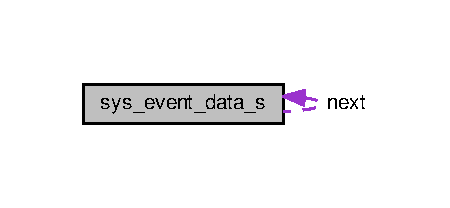
\includegraphics[width=216pt]{df/d2a/structsys__event__data__s__coll__graph}
\end{center}
\end{figure}
\subsection*{Data Fields}
\begin{DoxyCompactItemize}
\item 
void $\ast$ \hyperlink{structsys__event__data__s_a72c5ebbbee4b4509abcfb926d23f294f}{value}
\item 
\hyperlink{definitions_8h_a05f6b0ae8f6a6e135b0e290c25fe0e4e}{uint16} \hyperlink{structsys__event__data__s_a61e4846d66a617a9e5ed3602a3be63ef}{size}
\item 
struct \hyperlink{structsys__event__data__s}{sys\+\_\+event\+\_\+data\+\_\+s} $\ast$ \hyperlink{structsys__event__data__s_aa6f72c940fd46fc646876fe4271040a8}{next}
\end{DoxyCompactItemize}


\subsection{Detailed Description}
This struct contains data of the size {\bfseries size} at the memory of {\bfseries value}. It is a struct for a linked list. 

Definition at line 89 of file events.\+h.



\subsection{Field Documentation}
\hypertarget{structsys__event__data__s_aa6f72c940fd46fc646876fe4271040a8}{}\index{sys\+\_\+event\+\_\+data\+\_\+s@{sys\+\_\+event\+\_\+data\+\_\+s}!next@{next}}
\index{next@{next}!sys\+\_\+event\+\_\+data\+\_\+s@{sys\+\_\+event\+\_\+data\+\_\+s}}
\subsubsection[{next}]{\setlength{\rightskip}{0pt plus 5cm}struct {\bf sys\+\_\+event\+\_\+data\+\_\+s}$\ast$ sys\+\_\+event\+\_\+data\+\_\+s\+::next}\label{structsys__event__data__s_aa6f72c940fd46fc646876fe4271040a8}
pointer to the next element in the List 

Definition at line 93 of file events.\+h.

\hypertarget{structsys__event__data__s_a61e4846d66a617a9e5ed3602a3be63ef}{}\index{sys\+\_\+event\+\_\+data\+\_\+s@{sys\+\_\+event\+\_\+data\+\_\+s}!size@{size}}
\index{size@{size}!sys\+\_\+event\+\_\+data\+\_\+s@{sys\+\_\+event\+\_\+data\+\_\+s}}
\subsubsection[{size}]{\setlength{\rightskip}{0pt plus 5cm}{\bf uint16} sys\+\_\+event\+\_\+data\+\_\+s\+::size}\label{structsys__event__data__s_a61e4846d66a617a9e5ed3602a3be63ef}
size of the dransfered data (bytes) 

Definition at line 91 of file events.\+h.

\hypertarget{structsys__event__data__s_a72c5ebbbee4b4509abcfb926d23f294f}{}\index{sys\+\_\+event\+\_\+data\+\_\+s@{sys\+\_\+event\+\_\+data\+\_\+s}!value@{value}}
\index{value@{value}!sys\+\_\+event\+\_\+data\+\_\+s@{sys\+\_\+event\+\_\+data\+\_\+s}}
\subsubsection[{value}]{\setlength{\rightskip}{0pt plus 5cm}void$\ast$ sys\+\_\+event\+\_\+data\+\_\+s\+::value}\label{structsys__event__data__s_a72c5ebbbee4b4509abcfb926d23f294f}
pointer to the data transfered by an event 

Definition at line 90 of file events.\+h.



The documentation for this struct was generated from the following file\+:\begin{DoxyCompactItemize}
\item 
events/\hyperlink{events_8h}{events.\+h}\end{DoxyCompactItemize}

\hypertarget{structsys__i2c__message__s}{}\section{sys\+\_\+i2c\+\_\+message\+\_\+s Struct Reference}
\label{structsys__i2c__message__s}\index{sys\+\_\+i2c\+\_\+message\+\_\+s@{sys\+\_\+i2c\+\_\+message\+\_\+s}}


Linked list element of messages that need to be sent via I2\+C.  




{\ttfamily \#include $<$i2c\+\_\+data.\+h$>$}



Collaboration diagram for sys\+\_\+i2c\+\_\+message\+\_\+s\+:\nopagebreak
\begin{figure}[H]
\begin{center}
\leavevmode
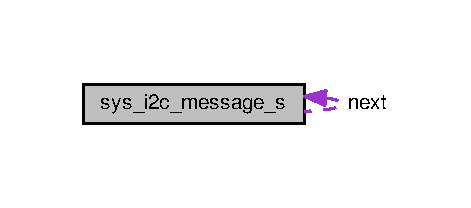
\includegraphics[width=226pt]{da/d56/structsys__i2c__message__s__coll__graph}
\end{center}
\end{figure}
\subsection*{Data Fields}
\begin{DoxyCompactItemize}
\item 
\hyperlink{definitions_8h_adde6aaee8457bee49c2a92621fe22b79}{uint8} \hyperlink{structsys__i2c__message__s_ad5b59be1fb573e7bc9b9b89da842c4aa}{i2c\+\_\+device\+\_\+address}
\item 
\hyperlink{definitions_8h_adde6aaee8457bee49c2a92621fe22b79}{uint8} $\ast$ \hyperlink{structsys__i2c__message__s_a49fa3d575b300fed2ea06cf331fa2180}{data}
\item 
\hyperlink{definitions_8h_a05f6b0ae8f6a6e135b0e290c25fe0e4e}{uint16} \hyperlink{structsys__i2c__message__s_a1846dd3ca2c59e4a1e68f2edb0c4b191}{length}
\item 
bool \hyperlink{structsys__i2c__message__s_ac3e159ca5b6afac6458dd2b7c991ce4f}{write}
\item 
\hyperlink{definitions_8h_a82fa7f76266ee1d687b76a44445f21ef}{p\+Byte\+Function} \hyperlink{structsys__i2c__message__s_a8632203d9a89893cb761ec37356c2288}{handler}
\item 
struct \hyperlink{structsys__i2c__message__s}{sys\+\_\+i2c\+\_\+message\+\_\+s} $\ast$ \hyperlink{structsys__i2c__message__s_aa435a9b8a1c7fabb600fd1394931a9a8}{next}
\end{DoxyCompactItemize}


\subsection{Detailed Description}
Linked list element of messages that need to be sent via I2\+C. 

Definition at line 32 of file i2c\+\_\+data.\+h.



\subsection{Field Documentation}
\hypertarget{structsys__i2c__message__s_a49fa3d575b300fed2ea06cf331fa2180}{}\index{sys\+\_\+i2c\+\_\+message\+\_\+s@{sys\+\_\+i2c\+\_\+message\+\_\+s}!data@{data}}
\index{data@{data}!sys\+\_\+i2c\+\_\+message\+\_\+s@{sys\+\_\+i2c\+\_\+message\+\_\+s}}
\subsubsection[{data}]{\setlength{\rightskip}{0pt plus 5cm}{\bf uint8}$\ast$ sys\+\_\+i2c\+\_\+message\+\_\+s\+::data}\label{structsys__i2c__message__s_a49fa3d575b300fed2ea06cf331fa2180}


Definition at line 34 of file i2c\+\_\+data.\+h.

\hypertarget{structsys__i2c__message__s_a8632203d9a89893cb761ec37356c2288}{}\index{sys\+\_\+i2c\+\_\+message\+\_\+s@{sys\+\_\+i2c\+\_\+message\+\_\+s}!handler@{handler}}
\index{handler@{handler}!sys\+\_\+i2c\+\_\+message\+\_\+s@{sys\+\_\+i2c\+\_\+message\+\_\+s}}
\subsubsection[{handler}]{\setlength{\rightskip}{0pt plus 5cm}{\bf p\+Byte\+Function} sys\+\_\+i2c\+\_\+message\+\_\+s\+::handler}\label{structsys__i2c__message__s_a8632203d9a89893cb761ec37356c2288}


Definition at line 37 of file i2c\+\_\+data.\+h.

\hypertarget{structsys__i2c__message__s_ad5b59be1fb573e7bc9b9b89da842c4aa}{}\index{sys\+\_\+i2c\+\_\+message\+\_\+s@{sys\+\_\+i2c\+\_\+message\+\_\+s}!i2c\+\_\+device\+\_\+address@{i2c\+\_\+device\+\_\+address}}
\index{i2c\+\_\+device\+\_\+address@{i2c\+\_\+device\+\_\+address}!sys\+\_\+i2c\+\_\+message\+\_\+s@{sys\+\_\+i2c\+\_\+message\+\_\+s}}
\subsubsection[{i2c\+\_\+device\+\_\+address}]{\setlength{\rightskip}{0pt plus 5cm}{\bf uint8} sys\+\_\+i2c\+\_\+message\+\_\+s\+::i2c\+\_\+device\+\_\+address}\label{structsys__i2c__message__s_ad5b59be1fb573e7bc9b9b89da842c4aa}


Definition at line 33 of file i2c\+\_\+data.\+h.

\hypertarget{structsys__i2c__message__s_a1846dd3ca2c59e4a1e68f2edb0c4b191}{}\index{sys\+\_\+i2c\+\_\+message\+\_\+s@{sys\+\_\+i2c\+\_\+message\+\_\+s}!length@{length}}
\index{length@{length}!sys\+\_\+i2c\+\_\+message\+\_\+s@{sys\+\_\+i2c\+\_\+message\+\_\+s}}
\subsubsection[{length}]{\setlength{\rightskip}{0pt plus 5cm}{\bf uint16} sys\+\_\+i2c\+\_\+message\+\_\+s\+::length}\label{structsys__i2c__message__s_a1846dd3ca2c59e4a1e68f2edb0c4b191}


Definition at line 35 of file i2c\+\_\+data.\+h.

\hypertarget{structsys__i2c__message__s_aa435a9b8a1c7fabb600fd1394931a9a8}{}\index{sys\+\_\+i2c\+\_\+message\+\_\+s@{sys\+\_\+i2c\+\_\+message\+\_\+s}!next@{next}}
\index{next@{next}!sys\+\_\+i2c\+\_\+message\+\_\+s@{sys\+\_\+i2c\+\_\+message\+\_\+s}}
\subsubsection[{next}]{\setlength{\rightskip}{0pt plus 5cm}struct {\bf sys\+\_\+i2c\+\_\+message\+\_\+s}$\ast$ sys\+\_\+i2c\+\_\+message\+\_\+s\+::next}\label{structsys__i2c__message__s_aa435a9b8a1c7fabb600fd1394931a9a8}


Definition at line 38 of file i2c\+\_\+data.\+h.

\hypertarget{structsys__i2c__message__s_ac3e159ca5b6afac6458dd2b7c991ce4f}{}\index{sys\+\_\+i2c\+\_\+message\+\_\+s@{sys\+\_\+i2c\+\_\+message\+\_\+s}!write@{write}}
\index{write@{write}!sys\+\_\+i2c\+\_\+message\+\_\+s@{sys\+\_\+i2c\+\_\+message\+\_\+s}}
\subsubsection[{write}]{\setlength{\rightskip}{0pt plus 5cm}bool sys\+\_\+i2c\+\_\+message\+\_\+s\+::write}\label{structsys__i2c__message__s_ac3e159ca5b6afac6458dd2b7c991ce4f}


Definition at line 36 of file i2c\+\_\+data.\+h.



The documentation for this struct was generated from the following file\+:\begin{DoxyCompactItemize}
\item 
platform/e-\/puck/\hyperlink{i2c__data_8h}{i2c\+\_\+data.\+h}\end{DoxyCompactItemize}

\hypertarget{structsys__motors__s}{}\section{sys\+\_\+motors\+\_\+s Struct Reference}
\label{structsys__motors__s}\index{sys\+\_\+motors\+\_\+s@{sys\+\_\+motors\+\_\+s}}


This struct contains speed for motors.  


\subsection*{Data Fields}
\begin{DoxyCompactItemize}
\item 
\hyperlink{definitions_8h_a74df79fde3c518e55b29ce6360a9c76e}{sint16} \hyperlink{structsys__motors__s_af052a7c6ad50ff8e0acaa8293b37f659}{speed}
\end{DoxyCompactItemize}


\subsection{Detailed Description}
This struct contains speed for motors. 

Definition at line 33 of file motors.\+c.



\subsection{Field Documentation}
\hypertarget{structsys__motors__s_af052a7c6ad50ff8e0acaa8293b37f659}{}\index{sys\+\_\+motors\+\_\+s@{sys\+\_\+motors\+\_\+s}!speed@{speed}}
\index{speed@{speed}!sys\+\_\+motors\+\_\+s@{sys\+\_\+motors\+\_\+s}}
\subsubsection[{speed}]{\setlength{\rightskip}{0pt plus 5cm}{\bf sint16} sys\+\_\+motors\+\_\+s\+::speed}\label{structsys__motors__s_af052a7c6ad50ff8e0acaa8293b37f659}


Definition at line 34 of file motors.\+c.



The documentation for this struct was generated from the following file\+:\begin{DoxyCompactItemize}
\item 
platform/e-\/puck/\hyperlink{motors_8c}{motors.\+c}\end{DoxyCompactItemize}

\hypertarget{structsys__occured__event__s}{}\section{sys\+\_\+occured\+\_\+event\+\_\+s Struct Reference}
\label{structsys__occured__event__s}\index{sys\+\_\+occured\+\_\+event\+\_\+s@{sys\+\_\+occured\+\_\+event\+\_\+s}}


List of occured events.  




{\ttfamily \#include $<$data.\+h$>$}



Collaboration diagram for sys\+\_\+occured\+\_\+event\+\_\+s\+:\nopagebreak
\begin{figure}[H]
\begin{center}
\leavevmode
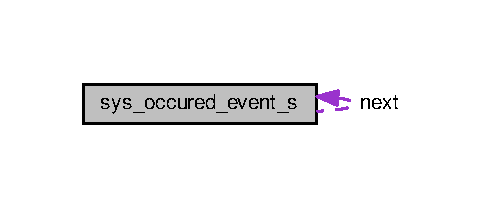
\includegraphics[width=232pt]{d1/d19/structsys__occured__event__s__coll__graph}
\end{center}
\end{figure}
\subsection*{Data Fields}
\begin{DoxyCompactItemize}
\item 
\hyperlink{definitions_8h_a05f6b0ae8f6a6e135b0e290c25fe0e4e}{uint16} \hyperlink{structsys__occured__event__s_a2bc2b2ee398582222728db5ad4aea1de}{event\+I\+D}
\item 
struct \hyperlink{structsys__occured__event__s}{sys\+\_\+occured\+\_\+event\+\_\+s} $\ast$ \hyperlink{structsys__occured__event__s_a5279262bb3a0710e84ecf6199dbca28e}{next}
\end{DoxyCompactItemize}


\subsection{Detailed Description}
List of occured events. 

This struct sores the event I\+D of an occurred event 

Definition at line 34 of file data.\+h.



\subsection{Field Documentation}
\hypertarget{structsys__occured__event__s_a2bc2b2ee398582222728db5ad4aea1de}{}\index{sys\+\_\+occured\+\_\+event\+\_\+s@{sys\+\_\+occured\+\_\+event\+\_\+s}!event\+I\+D@{event\+I\+D}}
\index{event\+I\+D@{event\+I\+D}!sys\+\_\+occured\+\_\+event\+\_\+s@{sys\+\_\+occured\+\_\+event\+\_\+s}}
\subsubsection[{event\+I\+D}]{\setlength{\rightskip}{0pt plus 5cm}{\bf uint16} sys\+\_\+occured\+\_\+event\+\_\+s\+::event\+I\+D}\label{structsys__occured__event__s_a2bc2b2ee398582222728db5ad4aea1de}


Definition at line 35 of file data.\+h.

\hypertarget{structsys__occured__event__s_a5279262bb3a0710e84ecf6199dbca28e}{}\index{sys\+\_\+occured\+\_\+event\+\_\+s@{sys\+\_\+occured\+\_\+event\+\_\+s}!next@{next}}
\index{next@{next}!sys\+\_\+occured\+\_\+event\+\_\+s@{sys\+\_\+occured\+\_\+event\+\_\+s}}
\subsubsection[{next}]{\setlength{\rightskip}{0pt plus 5cm}struct {\bf sys\+\_\+occured\+\_\+event\+\_\+s}$\ast$ sys\+\_\+occured\+\_\+event\+\_\+s\+::next}\label{structsys__occured__event__s_a5279262bb3a0710e84ecf6199dbca28e}


Definition at line 37 of file data.\+h.



The documentation for this struct was generated from the following file\+:\begin{DoxyCompactItemize}
\item 
processes/\hyperlink{data_8h}{data.\+h}\end{DoxyCompactItemize}

\hypertarget{structsys__periodical__IOHandler__s}{}\section{sys\+\_\+periodical\+\_\+\+I\+O\+Handler\+\_\+s Struct Reference}
\label{structsys__periodical__IOHandler__s}\index{sys\+\_\+periodical\+\_\+\+I\+O\+Handler\+\_\+s@{sys\+\_\+periodical\+\_\+\+I\+O\+Handler\+\_\+s}}


{\ttfamily \#include $<$io\+\_\+\+H\+D\+I.\+h$>$}



Collaboration diagram for sys\+\_\+periodical\+\_\+\+I\+O\+Handler\+\_\+s\+:\nopagebreak
\begin{figure}[H]
\begin{center}
\leavevmode
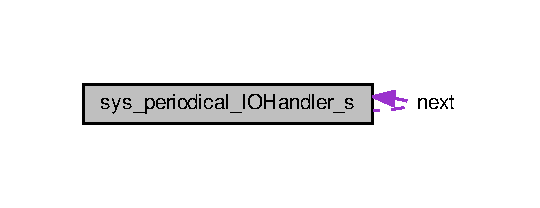
\includegraphics[width=259pt]{db/d16/structsys__periodical__IOHandler__s__coll__graph}
\end{center}
\end{figure}
\subsection*{Data Fields}
\begin{DoxyCompactItemize}
\item 
\hyperlink{definitions_8h_aed53e618f2025481fbe48a5098f70079}{p\+Function} \hyperlink{structsys__periodical__IOHandler__s_af22c738940f827dc20853e9e0edc0a56}{function}
\item 
struct \hyperlink{structsys__periodical__IOHandler__s}{sys\+\_\+periodical\+\_\+\+I\+O\+Handler\+\_\+s} $\ast$ \hyperlink{structsys__periodical__IOHandler__s_a36ad85ffbae299cfa418f69b6f2d745e}{next}
\end{DoxyCompactItemize}


\subsection{Detailed Description}


Definition at line 28 of file io\+\_\+\+H\+D\+I.\+h.



\subsection{Field Documentation}
\hypertarget{structsys__periodical__IOHandler__s_af22c738940f827dc20853e9e0edc0a56}{}\index{sys\+\_\+periodical\+\_\+\+I\+O\+Handler\+\_\+s@{sys\+\_\+periodical\+\_\+\+I\+O\+Handler\+\_\+s}!function@{function}}
\index{function@{function}!sys\+\_\+periodical\+\_\+\+I\+O\+Handler\+\_\+s@{sys\+\_\+periodical\+\_\+\+I\+O\+Handler\+\_\+s}}
\subsubsection[{function}]{\setlength{\rightskip}{0pt plus 5cm}{\bf p\+Function} sys\+\_\+periodical\+\_\+\+I\+O\+Handler\+\_\+s\+::function}\label{structsys__periodical__IOHandler__s_af22c738940f827dc20853e9e0edc0a56}


Definition at line 29 of file io\+\_\+\+H\+D\+I.\+h.

\hypertarget{structsys__periodical__IOHandler__s_a36ad85ffbae299cfa418f69b6f2d745e}{}\index{sys\+\_\+periodical\+\_\+\+I\+O\+Handler\+\_\+s@{sys\+\_\+periodical\+\_\+\+I\+O\+Handler\+\_\+s}!next@{next}}
\index{next@{next}!sys\+\_\+periodical\+\_\+\+I\+O\+Handler\+\_\+s@{sys\+\_\+periodical\+\_\+\+I\+O\+Handler\+\_\+s}}
\subsubsection[{next}]{\setlength{\rightskip}{0pt plus 5cm}struct {\bf sys\+\_\+periodical\+\_\+\+I\+O\+Handler\+\_\+s}$\ast$ sys\+\_\+periodical\+\_\+\+I\+O\+Handler\+\_\+s\+::next}\label{structsys__periodical__IOHandler__s_a36ad85ffbae299cfa418f69b6f2d745e}


Definition at line 31 of file io\+\_\+\+H\+D\+I.\+h.



The documentation for this struct was generated from the following file\+:\begin{DoxyCompactItemize}
\item 
platform/e-\/puck/\hyperlink{io__HDI_8h}{io\+\_\+\+H\+D\+I.\+h}\end{DoxyCompactItemize}

\hypertarget{structsys__process__control__block__list__element__s}{}\section{sys\+\_\+process\+\_\+control\+\_\+block\+\_\+list\+\_\+element\+\_\+s Struct Reference}
\label{structsys__process__control__block__list__element__s}\index{sys\+\_\+process\+\_\+control\+\_\+block\+\_\+list\+\_\+element\+\_\+s@{sys\+\_\+process\+\_\+control\+\_\+block\+\_\+list\+\_\+element\+\_\+s}}


Double linked list element containing sys\+\_\+process\+\_\+control\+\_\+block.  




{\ttfamily \#include $<$data.\+h$>$}



Collaboration diagram for sys\+\_\+process\+\_\+control\+\_\+block\+\_\+list\+\_\+element\+\_\+s\+:
% FIG 0
\subsection*{Data Fields}
\begin{DoxyCompactItemize}
\item 
\hyperlink{data_8h_a4a97a9fe481ab1cef2c0bb4c799431d0}{sys\+\_\+process\+\_\+control\+\_\+block} \hyperlink{structsys__process__control__block__list__element__s_a31a8928210b29e097924862367ae70a7}{pcb}
\item 
struct \hyperlink{structsys__process__control__block__list__element__s}{sys\+\_\+process\+\_\+control\+\_\+block\+\_\+list\+\_\+element\+\_\+s} $\ast$ \hyperlink{structsys__process__control__block__list__element__s_a91a80f7180ef47545efc44c1f94d5fb7}{previous}
\item 
struct \hyperlink{structsys__process__control__block__list__element__s}{sys\+\_\+process\+\_\+control\+\_\+block\+\_\+list\+\_\+element\+\_\+s} $\ast$ \hyperlink{structsys__process__control__block__list__element__s_a1f16ad20706b2be26e3ed97088b6d2f2}{next}
\end{DoxyCompactItemize}


\subsection{Detailed Description}
Double linked list element containing sys\+\_\+process\+\_\+control\+\_\+block. 

It is a double linked list element containing the P\+C\+B of a process 

Definition at line 77 of file data.\+h.



\subsection{Field Documentation}
\hypertarget{structsys__process__control__block__list__element__s_a1f16ad20706b2be26e3ed97088b6d2f2}{}\index{sys\+\_\+process\+\_\+control\+\_\+block\+\_\+list\+\_\+element\+\_\+s@{sys\+\_\+process\+\_\+control\+\_\+block\+\_\+list\+\_\+element\+\_\+s}!next@{next}}
\index{next@{next}!sys\+\_\+process\+\_\+control\+\_\+block\+\_\+list\+\_\+element\+\_\+s@{sys\+\_\+process\+\_\+control\+\_\+block\+\_\+list\+\_\+element\+\_\+s}}
\subsubsection[{next}]{\setlength{\rightskip}{0pt plus 5cm}struct {\bf sys\+\_\+process\+\_\+control\+\_\+block\+\_\+list\+\_\+element\+\_\+s}$\ast$ sys\+\_\+process\+\_\+control\+\_\+block\+\_\+list\+\_\+element\+\_\+s\+::next}\label{structsys__process__control__block__list__element__s_a1f16ad20706b2be26e3ed97088b6d2f2}


Definition at line 82 of file data.\+h.

\hypertarget{structsys__process__control__block__list__element__s_a31a8928210b29e097924862367ae70a7}{}\index{sys\+\_\+process\+\_\+control\+\_\+block\+\_\+list\+\_\+element\+\_\+s@{sys\+\_\+process\+\_\+control\+\_\+block\+\_\+list\+\_\+element\+\_\+s}!pcb@{pcb}}
\index{pcb@{pcb}!sys\+\_\+process\+\_\+control\+\_\+block\+\_\+list\+\_\+element\+\_\+s@{sys\+\_\+process\+\_\+control\+\_\+block\+\_\+list\+\_\+element\+\_\+s}}
\subsubsection[{pcb}]{\setlength{\rightskip}{0pt plus 5cm}{\bf sys\+\_\+process\+\_\+control\+\_\+block} sys\+\_\+process\+\_\+control\+\_\+block\+\_\+list\+\_\+element\+\_\+s\+::pcb}\label{structsys__process__control__block__list__element__s_a31a8928210b29e097924862367ae70a7}


Definition at line 79 of file data.\+h.

\hypertarget{structsys__process__control__block__list__element__s_a91a80f7180ef47545efc44c1f94d5fb7}{}\index{sys\+\_\+process\+\_\+control\+\_\+block\+\_\+list\+\_\+element\+\_\+s@{sys\+\_\+process\+\_\+control\+\_\+block\+\_\+list\+\_\+element\+\_\+s}!previous@{previous}}
\index{previous@{previous}!sys\+\_\+process\+\_\+control\+\_\+block\+\_\+list\+\_\+element\+\_\+s@{sys\+\_\+process\+\_\+control\+\_\+block\+\_\+list\+\_\+element\+\_\+s}}
\subsubsection[{previous}]{\setlength{\rightskip}{0pt plus 5cm}struct {\bf sys\+\_\+process\+\_\+control\+\_\+block\+\_\+list\+\_\+element\+\_\+s}$\ast$ sys\+\_\+process\+\_\+control\+\_\+block\+\_\+list\+\_\+element\+\_\+s\+::previous}\label{structsys__process__control__block__list__element__s_a91a80f7180ef47545efc44c1f94d5fb7}


Definition at line 81 of file data.\+h.



The documentation for this struct was generated from the following file\+:\begin{DoxyCompactItemize}
\item 
processes/\hyperlink{data_8h}{data.\+h}\end{DoxyCompactItemize}

\hypertarget{structsys__process__control__block__s}{}\section{sys\+\_\+process\+\_\+control\+\_\+block\+\_\+s Struct Reference}
\label{structsys__process__control__block__s}\index{sys\+\_\+process\+\_\+control\+\_\+block\+\_\+s@{sys\+\_\+process\+\_\+control\+\_\+block\+\_\+s}}


Process Control Block for the processes.  




{\ttfamily \#include $<$data.\+h$>$}



Collaboration diagram for sys\+\_\+process\+\_\+control\+\_\+block\+\_\+s\+:\nopagebreak
\begin{figure}[H]
\begin{center}
\leavevmode
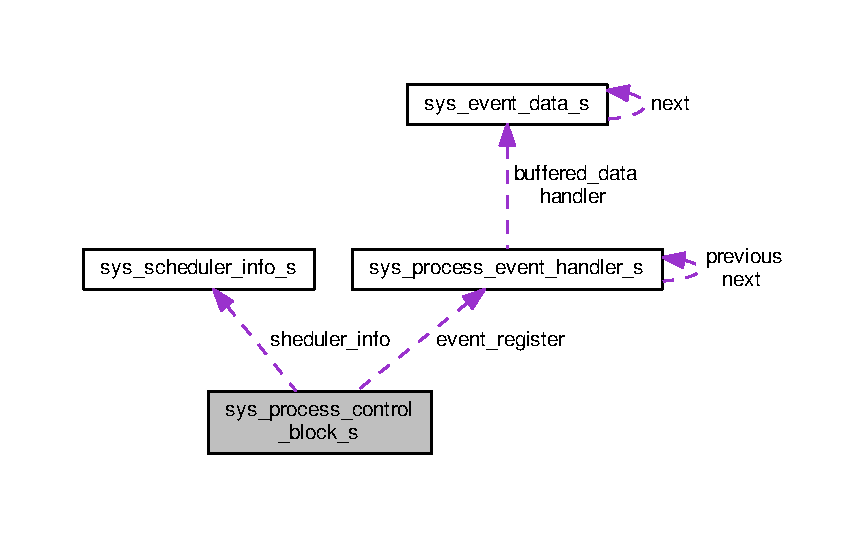
\includegraphics[width=350pt]{d5/d90/structsys__process__control__block__s__coll__graph}
\end{center}
\end{figure}
\subsection*{Data Fields}
\begin{DoxyCompactItemize}
\item 
\hyperlink{definitions_8h_a05f6b0ae8f6a6e135b0e290c25fe0e4e}{uint16} \hyperlink{structsys__process__control__block__s_a3f7ec6be0e16d1ae6b123a9b2bbb7176}{process\+\_\+\+I\+D}
\item 
\hyperlink{definitions_8h_a05f6b0ae8f6a6e135b0e290c25fe0e4e}{uint16} \hyperlink{structsys__process__control__block__s_a524ae2611a8aeb602c9c3ad78f4cae97}{stack\+Pointer}
\item 
\hyperlink{definitions_8h_a05f6b0ae8f6a6e135b0e290c25fe0e4e}{uint16} \hyperlink{structsys__process__control__block__s_aef61433a4fe380bd38c45fe3ea36433c}{frame\+Pointer}
\item 
\hyperlink{definitions_8h_a05f6b0ae8f6a6e135b0e290c25fe0e4e}{uint16} \hyperlink{structsys__process__control__block__s_a6ace28a95ee3d1ae4f0e36aa2675cf51}{stack\+Pointer\+Limit}
\item 
\hyperlink{scheduler_8h_aa491087633867d367d0f0c63f75ac41a}{sys\+\_\+scheduler\+\_\+info} \hyperlink{structsys__process__control__block__s_a0ef282f8acb4718b5a896e3c7d693a4a}{sheduler\+\_\+info}
\item 
\hyperlink{data_8h_a8840f47ed02e5b3b5b9ad35c55057a45}{sys\+\_\+process\+\_\+event\+\_\+handler} $\ast$ \hyperlink{structsys__process__control__block__s_a85bf797910e44aee733a9cc53db76728}{event\+\_\+register}
\item 
\hyperlink{definitions_8h_a05f6b0ae8f6a6e135b0e290c25fe0e4e}{uint16} $\ast$ \hyperlink{structsys__process__control__block__s_a094b1d3add4317d0100c53c8bdc26553}{process\+\_\+stack}
\end{DoxyCompactItemize}


\subsection{Detailed Description}
Process Control Block for the processes. 

This struct sores all information of the current state of a process 

Definition at line 58 of file data.\+h.



\subsection{Field Documentation}
\hypertarget{structsys__process__control__block__s_a85bf797910e44aee733a9cc53db76728}{}\index{sys\+\_\+process\+\_\+control\+\_\+block\+\_\+s@{sys\+\_\+process\+\_\+control\+\_\+block\+\_\+s}!event\+\_\+register@{event\+\_\+register}}
\index{event\+\_\+register@{event\+\_\+register}!sys\+\_\+process\+\_\+control\+\_\+block\+\_\+s@{sys\+\_\+process\+\_\+control\+\_\+block\+\_\+s}}
\subsubsection[{event\+\_\+register}]{\setlength{\rightskip}{0pt plus 5cm}{\bf sys\+\_\+process\+\_\+event\+\_\+handler}$\ast$ sys\+\_\+process\+\_\+control\+\_\+block\+\_\+s\+::event\+\_\+register}\label{structsys__process__control__block__s_a85bf797910e44aee733a9cc53db76728}


Definition at line 66 of file data.\+h.

\hypertarget{structsys__process__control__block__s_aef61433a4fe380bd38c45fe3ea36433c}{}\index{sys\+\_\+process\+\_\+control\+\_\+block\+\_\+s@{sys\+\_\+process\+\_\+control\+\_\+block\+\_\+s}!frame\+Pointer@{frame\+Pointer}}
\index{frame\+Pointer@{frame\+Pointer}!sys\+\_\+process\+\_\+control\+\_\+block\+\_\+s@{sys\+\_\+process\+\_\+control\+\_\+block\+\_\+s}}
\subsubsection[{frame\+Pointer}]{\setlength{\rightskip}{0pt plus 5cm}{\bf uint16} sys\+\_\+process\+\_\+control\+\_\+block\+\_\+s\+::frame\+Pointer}\label{structsys__process__control__block__s_aef61433a4fe380bd38c45fe3ea36433c}


Definition at line 62 of file data.\+h.

\hypertarget{structsys__process__control__block__s_a3f7ec6be0e16d1ae6b123a9b2bbb7176}{}\index{sys\+\_\+process\+\_\+control\+\_\+block\+\_\+s@{sys\+\_\+process\+\_\+control\+\_\+block\+\_\+s}!process\+\_\+\+I\+D@{process\+\_\+\+I\+D}}
\index{process\+\_\+\+I\+D@{process\+\_\+\+I\+D}!sys\+\_\+process\+\_\+control\+\_\+block\+\_\+s@{sys\+\_\+process\+\_\+control\+\_\+block\+\_\+s}}
\subsubsection[{process\+\_\+\+I\+D}]{\setlength{\rightskip}{0pt plus 5cm}{\bf uint16} sys\+\_\+process\+\_\+control\+\_\+block\+\_\+s\+::process\+\_\+\+I\+D}\label{structsys__process__control__block__s_a3f7ec6be0e16d1ae6b123a9b2bbb7176}


Definition at line 60 of file data.\+h.

\hypertarget{structsys__process__control__block__s_a094b1d3add4317d0100c53c8bdc26553}{}\index{sys\+\_\+process\+\_\+control\+\_\+block\+\_\+s@{sys\+\_\+process\+\_\+control\+\_\+block\+\_\+s}!process\+\_\+stack@{process\+\_\+stack}}
\index{process\+\_\+stack@{process\+\_\+stack}!sys\+\_\+process\+\_\+control\+\_\+block\+\_\+s@{sys\+\_\+process\+\_\+control\+\_\+block\+\_\+s}}
\subsubsection[{process\+\_\+stack}]{\setlength{\rightskip}{0pt plus 5cm}{\bf uint16}$\ast$ sys\+\_\+process\+\_\+control\+\_\+block\+\_\+s\+::process\+\_\+stack}\label{structsys__process__control__block__s_a094b1d3add4317d0100c53c8bdc26553}


Definition at line 68 of file data.\+h.

\hypertarget{structsys__process__control__block__s_a0ef282f8acb4718b5a896e3c7d693a4a}{}\index{sys\+\_\+process\+\_\+control\+\_\+block\+\_\+s@{sys\+\_\+process\+\_\+control\+\_\+block\+\_\+s}!sheduler\+\_\+info@{sheduler\+\_\+info}}
\index{sheduler\+\_\+info@{sheduler\+\_\+info}!sys\+\_\+process\+\_\+control\+\_\+block\+\_\+s@{sys\+\_\+process\+\_\+control\+\_\+block\+\_\+s}}
\subsubsection[{sheduler\+\_\+info}]{\setlength{\rightskip}{0pt plus 5cm}{\bf sys\+\_\+scheduler\+\_\+info} sys\+\_\+process\+\_\+control\+\_\+block\+\_\+s\+::sheduler\+\_\+info}\label{structsys__process__control__block__s_a0ef282f8acb4718b5a896e3c7d693a4a}


Definition at line 65 of file data.\+h.

\hypertarget{structsys__process__control__block__s_a524ae2611a8aeb602c9c3ad78f4cae97}{}\index{sys\+\_\+process\+\_\+control\+\_\+block\+\_\+s@{sys\+\_\+process\+\_\+control\+\_\+block\+\_\+s}!stack\+Pointer@{stack\+Pointer}}
\index{stack\+Pointer@{stack\+Pointer}!sys\+\_\+process\+\_\+control\+\_\+block\+\_\+s@{sys\+\_\+process\+\_\+control\+\_\+block\+\_\+s}}
\subsubsection[{stack\+Pointer}]{\setlength{\rightskip}{0pt plus 5cm}{\bf uint16} sys\+\_\+process\+\_\+control\+\_\+block\+\_\+s\+::stack\+Pointer}\label{structsys__process__control__block__s_a524ae2611a8aeb602c9c3ad78f4cae97}
Stack Pointer to T\+O\+P 

Definition at line 61 of file data.\+h.

\hypertarget{structsys__process__control__block__s_a6ace28a95ee3d1ae4f0e36aa2675cf51}{}\index{sys\+\_\+process\+\_\+control\+\_\+block\+\_\+s@{sys\+\_\+process\+\_\+control\+\_\+block\+\_\+s}!stack\+Pointer\+Limit@{stack\+Pointer\+Limit}}
\index{stack\+Pointer\+Limit@{stack\+Pointer\+Limit}!sys\+\_\+process\+\_\+control\+\_\+block\+\_\+s@{sys\+\_\+process\+\_\+control\+\_\+block\+\_\+s}}
\subsubsection[{stack\+Pointer\+Limit}]{\setlength{\rightskip}{0pt plus 5cm}{\bf uint16} sys\+\_\+process\+\_\+control\+\_\+block\+\_\+s\+::stack\+Pointer\+Limit}\label{structsys__process__control__block__s_a6ace28a95ee3d1ae4f0e36aa2675cf51}
Stack Pointer + M\+A\+X S\+I\+Z\+E 

Definition at line 63 of file data.\+h.



The documentation for this struct was generated from the following file\+:\begin{DoxyCompactItemize}
\item 
processes/\hyperlink{data_8h}{data.\+h}\end{DoxyCompactItemize}

\hypertarget{structsys__process__event__handler__s}{}\section{sys\+\_\+process\+\_\+event\+\_\+handler\+\_\+s Struct Reference}
\label{structsys__process__event__handler__s}\index{sys\+\_\+process\+\_\+event\+\_\+handler\+\_\+s@{sys\+\_\+process\+\_\+event\+\_\+handler\+\_\+s}}


List of process event-\/handlers.  




{\ttfamily \#include $<$data.\+h$>$}



Collaboration diagram for sys\+\_\+process\+\_\+event\+\_\+handler\+\_\+s\+:\nopagebreak
\begin{figure}[H]
\begin{center}
\leavevmode
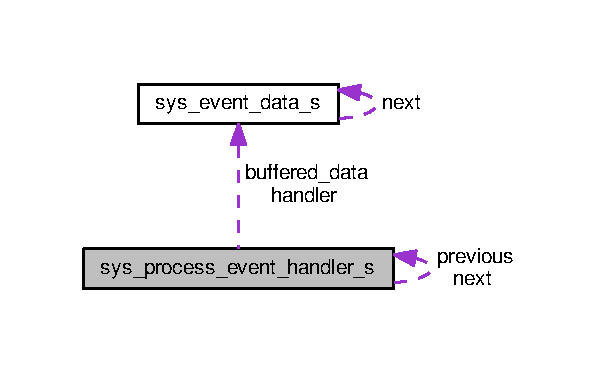
\includegraphics[width=287pt]{d8/d90/structsys__process__event__handler__s__coll__graph}
\end{center}
\end{figure}
\subsection*{Data Fields}
\begin{DoxyCompactItemize}
\item 
\hyperlink{definitions_8h_a05f6b0ae8f6a6e135b0e290c25fe0e4e}{uint16} \hyperlink{structsys__process__event__handler__s_a4b799aaf40561daed132a1a1d688ecd8}{event\+I\+D}
\item 
\hyperlink{events_8h_a38c799788eea576b2d878371da3d5385}{p\+Event\+Handler\+Function} \hyperlink{structsys__process__event__handler__s_a980eeb4cb54ac72cd3ebc38e391c40a5}{handler}
\item 
\hyperlink{events_8h_a653a4a4b7d9f5a65e1415365267a9d9e}{p\+Condition\+Function} \hyperlink{structsys__process__event__handler__s_a43ea89783cb8b5cfd0896410f1f7a691}{condition}
\item 
\hyperlink{events_8h_ae3a76ca1b349999a35d55f3224897b5f}{sys\+\_\+event\+\_\+data} $\ast$ \hyperlink{structsys__process__event__handler__s_adbcb330724f201fb328fb91d2c6353e3}{buffered\+\_\+data}
\item 
struct \hyperlink{structsys__process__event__handler__s}{sys\+\_\+process\+\_\+event\+\_\+handler\+\_\+s} $\ast$ \hyperlink{structsys__process__event__handler__s_abbb4742265dace5feffc2a1b05d5271c}{previous}
\item 
struct \hyperlink{structsys__process__event__handler__s}{sys\+\_\+process\+\_\+event\+\_\+handler\+\_\+s} $\ast$ \hyperlink{structsys__process__event__handler__s_abd718f866343f0a1e139c977bbae72b8}{next}
\end{DoxyCompactItemize}


\subsection{Detailed Description}
List of process event-\/handlers. 

This struct sores all information needed to decide if the event-\/handler is executed for the event (event\+I\+D). To store the event data and be executed, a condition has to be met. 

Definition at line 44 of file data.\+h.



\subsection{Field Documentation}
\hypertarget{structsys__process__event__handler__s_adbcb330724f201fb328fb91d2c6353e3}{}\index{sys\+\_\+process\+\_\+event\+\_\+handler\+\_\+s@{sys\+\_\+process\+\_\+event\+\_\+handler\+\_\+s}!buffered\+\_\+data@{buffered\+\_\+data}}
\index{buffered\+\_\+data@{buffered\+\_\+data}!sys\+\_\+process\+\_\+event\+\_\+handler\+\_\+s@{sys\+\_\+process\+\_\+event\+\_\+handler\+\_\+s}}
\subsubsection[{buffered\+\_\+data}]{\setlength{\rightskip}{0pt plus 5cm}{\bf sys\+\_\+event\+\_\+data}$\ast$ sys\+\_\+process\+\_\+event\+\_\+handler\+\_\+s\+::buffered\+\_\+data}\label{structsys__process__event__handler__s_adbcb330724f201fb328fb91d2c6353e3}
stores the data 

Definition at line 48 of file data.\+h.

\hypertarget{structsys__process__event__handler__s_a43ea89783cb8b5cfd0896410f1f7a691}{}\index{sys\+\_\+process\+\_\+event\+\_\+handler\+\_\+s@{sys\+\_\+process\+\_\+event\+\_\+handler\+\_\+s}!condition@{condition}}
\index{condition@{condition}!sys\+\_\+process\+\_\+event\+\_\+handler\+\_\+s@{sys\+\_\+process\+\_\+event\+\_\+handler\+\_\+s}}
\subsubsection[{condition}]{\setlength{\rightskip}{0pt plus 5cm}{\bf p\+Condition\+Function} sys\+\_\+process\+\_\+event\+\_\+handler\+\_\+s\+::condition}\label{structsys__process__event__handler__s_a43ea89783cb8b5cfd0896410f1f7a691}
Pointer to function which checks if the event-\/handler has to be executed (true) or nor (false) 

Definition at line 47 of file data.\+h.

\hypertarget{structsys__process__event__handler__s_a4b799aaf40561daed132a1a1d688ecd8}{}\index{sys\+\_\+process\+\_\+event\+\_\+handler\+\_\+s@{sys\+\_\+process\+\_\+event\+\_\+handler\+\_\+s}!event\+I\+D@{event\+I\+D}}
\index{event\+I\+D@{event\+I\+D}!sys\+\_\+process\+\_\+event\+\_\+handler\+\_\+s@{sys\+\_\+process\+\_\+event\+\_\+handler\+\_\+s}}
\subsubsection[{event\+I\+D}]{\setlength{\rightskip}{0pt plus 5cm}{\bf uint16} sys\+\_\+process\+\_\+event\+\_\+handler\+\_\+s\+::event\+I\+D}\label{structsys__process__event__handler__s_a4b799aaf40561daed132a1a1d688ecd8}


Definition at line 45 of file data.\+h.

\hypertarget{structsys__process__event__handler__s_a980eeb4cb54ac72cd3ebc38e391c40a5}{}\index{sys\+\_\+process\+\_\+event\+\_\+handler\+\_\+s@{sys\+\_\+process\+\_\+event\+\_\+handler\+\_\+s}!handler@{handler}}
\index{handler@{handler}!sys\+\_\+process\+\_\+event\+\_\+handler\+\_\+s@{sys\+\_\+process\+\_\+event\+\_\+handler\+\_\+s}}
\subsubsection[{handler}]{\setlength{\rightskip}{0pt plus 5cm}{\bf p\+Event\+Handler\+Function} sys\+\_\+process\+\_\+event\+\_\+handler\+\_\+s\+::handler}\label{structsys__process__event__handler__s_a980eeb4cb54ac72cd3ebc38e391c40a5}
Pointer to function which computes the evnt data 

Definition at line 46 of file data.\+h.

\hypertarget{structsys__process__event__handler__s_abd718f866343f0a1e139c977bbae72b8}{}\index{sys\+\_\+process\+\_\+event\+\_\+handler\+\_\+s@{sys\+\_\+process\+\_\+event\+\_\+handler\+\_\+s}!next@{next}}
\index{next@{next}!sys\+\_\+process\+\_\+event\+\_\+handler\+\_\+s@{sys\+\_\+process\+\_\+event\+\_\+handler\+\_\+s}}
\subsubsection[{next}]{\setlength{\rightskip}{0pt plus 5cm}struct {\bf sys\+\_\+process\+\_\+event\+\_\+handler\+\_\+s}$\ast$ sys\+\_\+process\+\_\+event\+\_\+handler\+\_\+s\+::next}\label{structsys__process__event__handler__s_abd718f866343f0a1e139c977bbae72b8}


Definition at line 51 of file data.\+h.

\hypertarget{structsys__process__event__handler__s_abbb4742265dace5feffc2a1b05d5271c}{}\index{sys\+\_\+process\+\_\+event\+\_\+handler\+\_\+s@{sys\+\_\+process\+\_\+event\+\_\+handler\+\_\+s}!previous@{previous}}
\index{previous@{previous}!sys\+\_\+process\+\_\+event\+\_\+handler\+\_\+s@{sys\+\_\+process\+\_\+event\+\_\+handler\+\_\+s}}
\subsubsection[{previous}]{\setlength{\rightskip}{0pt plus 5cm}struct {\bf sys\+\_\+process\+\_\+event\+\_\+handler\+\_\+s}$\ast$ sys\+\_\+process\+\_\+event\+\_\+handler\+\_\+s\+::previous}\label{structsys__process__event__handler__s_abbb4742265dace5feffc2a1b05d5271c}


Definition at line 50 of file data.\+h.



The documentation for this struct was generated from the following file\+:\begin{DoxyCompactItemize}
\item 
processes/\hyperlink{data_8h}{data.\+h}\end{DoxyCompactItemize}

\hypertarget{structsys__registered__event__s}{}\section{sys\+\_\+registered\+\_\+event\+\_\+s Struct Reference}
\label{structsys__registered__event__s}\index{sys\+\_\+registered\+\_\+event\+\_\+s@{sys\+\_\+registered\+\_\+event\+\_\+s}}


A struct to store registered events. It also includes a list of processes that are subscribed to the registered event.  




Collaboration diagram for sys\+\_\+registered\+\_\+event\+\_\+s\+:\nopagebreak
\begin{figure}[H]
\begin{center}
\leavevmode
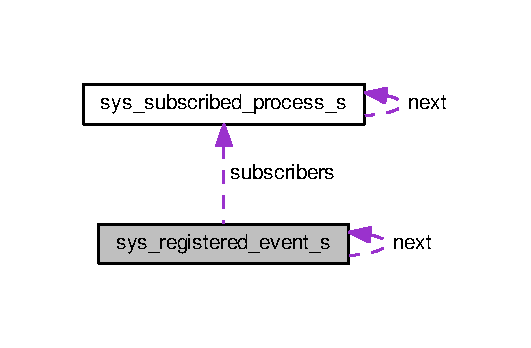
\includegraphics[width=255pt]{de/d55/structsys__registered__event__s__coll__graph}
\end{center}
\end{figure}
\subsection*{Data Fields}
\begin{DoxyCompactItemize}
\item 
\hyperlink{definitions_8h_a05f6b0ae8f6a6e135b0e290c25fe0e4e}{uint16} \hyperlink{structsys__registered__event__s_a44886c67a44aee553cbbbcd9903fcd39}{id}
\item 
\hyperlink{events_8c_a855a9b5c8c07fedd9f2a8bbf5ee9b4f0}{sys\+\_\+subscribed\+\_\+process} $\ast$ \hyperlink{structsys__registered__event__s_acea93fade98b2e5bd81cc9b6ed35388d}{subscribers}
\item 
struct \hyperlink{structsys__registered__event__s}{sys\+\_\+registered\+\_\+event\+\_\+s} $\ast$ \hyperlink{structsys__registered__event__s_a084bfc795b0f5135b6439a28bf9920c1}{next}
\end{DoxyCompactItemize}


\subsection{Detailed Description}
A struct to store registered events. It also includes a list of processes that are subscribed to the registered event. 

Definition at line 32 of file events.\+c.



\subsection{Field Documentation}
\hypertarget{structsys__registered__event__s_a44886c67a44aee553cbbbcd9903fcd39}{}\index{sys\+\_\+registered\+\_\+event\+\_\+s@{sys\+\_\+registered\+\_\+event\+\_\+s}!id@{id}}
\index{id@{id}!sys\+\_\+registered\+\_\+event\+\_\+s@{sys\+\_\+registered\+\_\+event\+\_\+s}}
\subsubsection[{id}]{\setlength{\rightskip}{0pt plus 5cm}{\bf uint16} sys\+\_\+registered\+\_\+event\+\_\+s\+::id}\label{structsys__registered__event__s_a44886c67a44aee553cbbbcd9903fcd39}
event identifier 

Definition at line 33 of file events.\+c.

\hypertarget{structsys__registered__event__s_a084bfc795b0f5135b6439a28bf9920c1}{}\index{sys\+\_\+registered\+\_\+event\+\_\+s@{sys\+\_\+registered\+\_\+event\+\_\+s}!next@{next}}
\index{next@{next}!sys\+\_\+registered\+\_\+event\+\_\+s@{sys\+\_\+registered\+\_\+event\+\_\+s}}
\subsubsection[{next}]{\setlength{\rightskip}{0pt plus 5cm}struct {\bf sys\+\_\+registered\+\_\+event\+\_\+s}$\ast$ sys\+\_\+registered\+\_\+event\+\_\+s\+::next}\label{structsys__registered__event__s_a084bfc795b0f5135b6439a28bf9920c1}
pointer to the next element in the List 

Definition at line 35 of file events.\+c.

\hypertarget{structsys__registered__event__s_acea93fade98b2e5bd81cc9b6ed35388d}{}\index{sys\+\_\+registered\+\_\+event\+\_\+s@{sys\+\_\+registered\+\_\+event\+\_\+s}!subscribers@{subscribers}}
\index{subscribers@{subscribers}!sys\+\_\+registered\+\_\+event\+\_\+s@{sys\+\_\+registered\+\_\+event\+\_\+s}}
\subsubsection[{subscribers}]{\setlength{\rightskip}{0pt plus 5cm}{\bf sys\+\_\+subscribed\+\_\+process}$\ast$ sys\+\_\+registered\+\_\+event\+\_\+s\+::subscribers}\label{structsys__registered__event__s_acea93fade98b2e5bd81cc9b6ed35388d}
pointer to a list of subscribed processes 

Definition at line 34 of file events.\+c.



The documentation for this struct was generated from the following file\+:\begin{DoxyCompactItemize}
\item 
events/\hyperlink{events_8c}{events.\+c}\end{DoxyCompactItemize}

\hypertarget{structsys__rgb__pixel__s}{}\section{sys\+\_\+rgb\+\_\+pixel\+\_\+s Struct Reference}
\label{structsys__rgb__pixel__s}\index{sys\+\_\+rgb\+\_\+pixel\+\_\+s@{sys\+\_\+rgb\+\_\+pixel\+\_\+s}}


This bitfield contains the structure of the received pixel of a camera.  




{\ttfamily \#include $<$camera.\+h$>$}

\subsection*{Data Fields}
\begin{DoxyCompactItemize}
\item 
\hyperlink{definitions_8h_adde6aaee8457bee49c2a92621fe22b79}{uint8} \hyperlink{structsys__rgb__pixel__s_a8f0985f9f96d4c7a6723aa10dcacc93b}{red}\+: 5
\item 
\hyperlink{definitions_8h_adde6aaee8457bee49c2a92621fe22b79}{uint8} \hyperlink{structsys__rgb__pixel__s_aad4178b262be3365f99a3cadece2f528}{green}\+: 6
\item 
\hyperlink{definitions_8h_adde6aaee8457bee49c2a92621fe22b79}{uint8} \hyperlink{structsys__rgb__pixel__s_a92b6e3779404cee9fde835ba597f22c7}{blue}\+: 5
\end{DoxyCompactItemize}


\subsection{Detailed Description}
This bitfield contains the structure of the received pixel of a camera. 

Definition at line 57 of file camera.\+h.



\subsection{Field Documentation}
\hypertarget{structsys__rgb__pixel__s_a92b6e3779404cee9fde835ba597f22c7}{}\index{sys\+\_\+rgb\+\_\+pixel\+\_\+s@{sys\+\_\+rgb\+\_\+pixel\+\_\+s}!blue@{blue}}
\index{blue@{blue}!sys\+\_\+rgb\+\_\+pixel\+\_\+s@{sys\+\_\+rgb\+\_\+pixel\+\_\+s}}
\subsubsection[{blue}]{\setlength{\rightskip}{0pt plus 5cm}{\bf uint8} sys\+\_\+rgb\+\_\+pixel\+\_\+s\+::blue}\label{structsys__rgb__pixel__s_a92b6e3779404cee9fde835ba597f22c7}


Definition at line 60 of file camera.\+h.

\hypertarget{structsys__rgb__pixel__s_aad4178b262be3365f99a3cadece2f528}{}\index{sys\+\_\+rgb\+\_\+pixel\+\_\+s@{sys\+\_\+rgb\+\_\+pixel\+\_\+s}!green@{green}}
\index{green@{green}!sys\+\_\+rgb\+\_\+pixel\+\_\+s@{sys\+\_\+rgb\+\_\+pixel\+\_\+s}}
\subsubsection[{green}]{\setlength{\rightskip}{0pt plus 5cm}{\bf uint8} sys\+\_\+rgb\+\_\+pixel\+\_\+s\+::green}\label{structsys__rgb__pixel__s_aad4178b262be3365f99a3cadece2f528}


Definition at line 59 of file camera.\+h.

\hypertarget{structsys__rgb__pixel__s_a8f0985f9f96d4c7a6723aa10dcacc93b}{}\index{sys\+\_\+rgb\+\_\+pixel\+\_\+s@{sys\+\_\+rgb\+\_\+pixel\+\_\+s}!red@{red}}
\index{red@{red}!sys\+\_\+rgb\+\_\+pixel\+\_\+s@{sys\+\_\+rgb\+\_\+pixel\+\_\+s}}
\subsubsection[{red}]{\setlength{\rightskip}{0pt plus 5cm}{\bf uint8} sys\+\_\+rgb\+\_\+pixel\+\_\+s\+::red}\label{structsys__rgb__pixel__s_a8f0985f9f96d4c7a6723aa10dcacc93b}


Definition at line 58 of file camera.\+h.



The documentation for this struct was generated from the following file\+:\begin{DoxyCompactItemize}
\item 
platform/e-\/puck/\hyperlink{camera_8h}{camera.\+h}\end{DoxyCompactItemize}

\hypertarget{structsys__scheduler__info__s}{}\section{sys\+\_\+scheduler\+\_\+info\+\_\+s Struct Reference}
\label{structsys__scheduler__info__s}\index{sys\+\_\+scheduler\+\_\+info\+\_\+s@{sys\+\_\+scheduler\+\_\+info\+\_\+s}}


The scheduling information for each process.  




{\ttfamily \#include $<$scheduler.\+h$>$}

\subsection*{Data Fields}
\begin{DoxyCompactItemize}
\item 
unsigned short \hyperlink{structsys__scheduler__info__s_a95d0294a71162ffbd1e65fd381e54a6b}{state}
\item 
unsigned short \hyperlink{structsys__scheduler__info__s_ad04085351f98898a0631e07aba0338d6}{priority}
\end{DoxyCompactItemize}


\subsection{Detailed Description}
The scheduling information for each process. 

This struct defines all values wich are needed for the scheduling algorithm 

Definition at line 37 of file scheduler.\+h.



\subsection{Field Documentation}
\hypertarget{structsys__scheduler__info__s_ad04085351f98898a0631e07aba0338d6}{}\index{sys\+\_\+scheduler\+\_\+info\+\_\+s@{sys\+\_\+scheduler\+\_\+info\+\_\+s}!priority@{priority}}
\index{priority@{priority}!sys\+\_\+scheduler\+\_\+info\+\_\+s@{sys\+\_\+scheduler\+\_\+info\+\_\+s}}
\subsubsection[{priority}]{\setlength{\rightskip}{0pt plus 5cm}unsigned short sys\+\_\+scheduler\+\_\+info\+\_\+s\+::priority}\label{structsys__scheduler__info__s_ad04085351f98898a0631e07aba0338d6}
process priority level 

Definition at line 39 of file scheduler.\+h.

\hypertarget{structsys__scheduler__info__s_a95d0294a71162ffbd1e65fd381e54a6b}{}\index{sys\+\_\+scheduler\+\_\+info\+\_\+s@{sys\+\_\+scheduler\+\_\+info\+\_\+s}!state@{state}}
\index{state@{state}!sys\+\_\+scheduler\+\_\+info\+\_\+s@{sys\+\_\+scheduler\+\_\+info\+\_\+s}}
\subsubsection[{state}]{\setlength{\rightskip}{0pt plus 5cm}unsigned short sys\+\_\+scheduler\+\_\+info\+\_\+s\+::state}\label{structsys__scheduler__info__s_a95d0294a71162ffbd1e65fd381e54a6b}
Process state information 

Definition at line 38 of file scheduler.\+h.



The documentation for this struct was generated from the following file\+:\begin{DoxyCompactItemize}
\item 
processes/\hyperlink{scheduler_8h}{scheduler.\+h}\end{DoxyCompactItemize}

\hypertarget{structsys__subscribed__process__s}{}\section{sys\+\_\+subscribed\+\_\+process\+\_\+s Struct Reference}
\label{structsys__subscribed__process__s}\index{sys\+\_\+subscribed\+\_\+process\+\_\+s@{sys\+\_\+subscribed\+\_\+process\+\_\+s}}


A single linked list element containing the I\+D of a subscribed process.  




Collaboration diagram for sys\+\_\+subscribed\+\_\+process\+\_\+s\+:\nopagebreak
\begin{figure}[H]
\begin{center}
\leavevmode
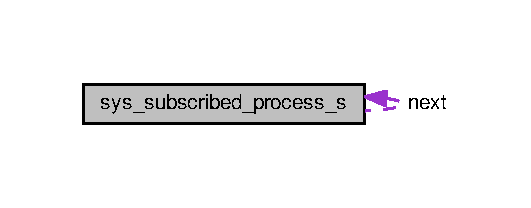
\includegraphics[width=255pt]{d8/d74/structsys__subscribed__process__s__coll__graph}
\end{center}
\end{figure}
\subsection*{Data Fields}
\begin{DoxyCompactItemize}
\item 
\hyperlink{definitions_8h_a05f6b0ae8f6a6e135b0e290c25fe0e4e}{uint16} \hyperlink{structsys__subscribed__process__s_a94e62af7fee25e53ea6c81cbb311783d}{pid}
\item 
struct \hyperlink{structsys__subscribed__process__s}{sys\+\_\+subscribed\+\_\+process\+\_\+s} $\ast$ \hyperlink{structsys__subscribed__process__s_abcf0ef070dc4fd0ba7165dfae52d7316}{next}
\end{DoxyCompactItemize}


\subsection{Detailed Description}
A single linked list element containing the I\+D of a subscribed process. 

Definition at line 24 of file events.\+c.



\subsection{Field Documentation}
\hypertarget{structsys__subscribed__process__s_abcf0ef070dc4fd0ba7165dfae52d7316}{}\index{sys\+\_\+subscribed\+\_\+process\+\_\+s@{sys\+\_\+subscribed\+\_\+process\+\_\+s}!next@{next}}
\index{next@{next}!sys\+\_\+subscribed\+\_\+process\+\_\+s@{sys\+\_\+subscribed\+\_\+process\+\_\+s}}
\subsubsection[{next}]{\setlength{\rightskip}{0pt plus 5cm}struct {\bf sys\+\_\+subscribed\+\_\+process\+\_\+s}$\ast$ sys\+\_\+subscribed\+\_\+process\+\_\+s\+::next}\label{structsys__subscribed__process__s_abcf0ef070dc4fd0ba7165dfae52d7316}
pointer to the next element in the List 

Definition at line 26 of file events.\+c.

\hypertarget{structsys__subscribed__process__s_a94e62af7fee25e53ea6c81cbb311783d}{}\index{sys\+\_\+subscribed\+\_\+process\+\_\+s@{sys\+\_\+subscribed\+\_\+process\+\_\+s}!pid@{pid}}
\index{pid@{pid}!sys\+\_\+subscribed\+\_\+process\+\_\+s@{sys\+\_\+subscribed\+\_\+process\+\_\+s}}
\subsubsection[{pid}]{\setlength{\rightskip}{0pt plus 5cm}{\bf uint16} sys\+\_\+subscribed\+\_\+process\+\_\+s\+::pid}\label{structsys__subscribed__process__s_a94e62af7fee25e53ea6c81cbb311783d}
process identifier 

Definition at line 25 of file events.\+c.



The documentation for this struct was generated from the following file\+:\begin{DoxyCompactItemize}
\item 
events/\hyperlink{events_8c}{events.\+c}\end{DoxyCompactItemize}

\hypertarget{structuart__tx__data__s}{}\section{uart\+\_\+tx\+\_\+data\+\_\+s Struct Reference}
\label{structuart__tx__data__s}\index{uart\+\_\+tx\+\_\+data\+\_\+s@{uart\+\_\+tx\+\_\+data\+\_\+s}}


{\ttfamily \#include $<$uart\+\_\+\+H\+D\+I.\+h$>$}



Collaboration diagram for uart\+\_\+tx\+\_\+data\+\_\+s\+:\nopagebreak
\begin{figure}[H]
\begin{center}
\leavevmode
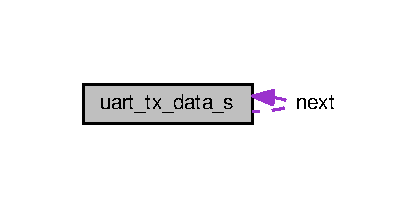
\includegraphics[width=201pt]{da/d8f/structuart__tx__data__s__coll__graph}
\end{center}
\end{figure}
\subsection*{Data Fields}
\begin{DoxyCompactItemize}
\item 
\hyperlink{definitions_8h_adde6aaee8457bee49c2a92621fe22b79}{uint8} $\ast$ \hyperlink{structuart__tx__data__s_a8c8a4dcb88914689fbcf3c605e7e086a}{data}
\item 
\hyperlink{definitions_8h_a05f6b0ae8f6a6e135b0e290c25fe0e4e}{uint16} \hyperlink{structuart__tx__data__s_a5f6561e844d7ba918becf2eeadfa7fdf}{length}
\item 
struct \hyperlink{structuart__tx__data__s}{uart\+\_\+tx\+\_\+data\+\_\+s} $\ast$ \hyperlink{structuart__tx__data__s_a1ca59d43b0ec489235518ce3037eb350}{next}
\end{DoxyCompactItemize}


\subsection{Detailed Description}
Linked list element to store the transmission data

This struct contains data and the amount of bytes that should be sent via U\+A\+R\+T1. 

Definition at line 47 of file uart\+\_\+\+H\+D\+I.\+h.



\subsection{Field Documentation}
\hypertarget{structuart__tx__data__s_a8c8a4dcb88914689fbcf3c605e7e086a}{}\index{uart\+\_\+tx\+\_\+data\+\_\+s@{uart\+\_\+tx\+\_\+data\+\_\+s}!data@{data}}
\index{data@{data}!uart\+\_\+tx\+\_\+data\+\_\+s@{uart\+\_\+tx\+\_\+data\+\_\+s}}
\subsubsection[{data}]{\setlength{\rightskip}{0pt plus 5cm}{\bf uint8}$\ast$ uart\+\_\+tx\+\_\+data\+\_\+s\+::data}\label{structuart__tx__data__s_a8c8a4dcb88914689fbcf3c605e7e086a}


Definition at line 48 of file uart\+\_\+\+H\+D\+I.\+h.

\hypertarget{structuart__tx__data__s_a5f6561e844d7ba918becf2eeadfa7fdf}{}\index{uart\+\_\+tx\+\_\+data\+\_\+s@{uart\+\_\+tx\+\_\+data\+\_\+s}!length@{length}}
\index{length@{length}!uart\+\_\+tx\+\_\+data\+\_\+s@{uart\+\_\+tx\+\_\+data\+\_\+s}}
\subsubsection[{length}]{\setlength{\rightskip}{0pt plus 5cm}{\bf uint16} uart\+\_\+tx\+\_\+data\+\_\+s\+::length}\label{structuart__tx__data__s_a5f6561e844d7ba918becf2eeadfa7fdf}


Definition at line 49 of file uart\+\_\+\+H\+D\+I.\+h.

\hypertarget{structuart__tx__data__s_a1ca59d43b0ec489235518ce3037eb350}{}\index{uart\+\_\+tx\+\_\+data\+\_\+s@{uart\+\_\+tx\+\_\+data\+\_\+s}!next@{next}}
\index{next@{next}!uart\+\_\+tx\+\_\+data\+\_\+s@{uart\+\_\+tx\+\_\+data\+\_\+s}}
\subsubsection[{next}]{\setlength{\rightskip}{0pt plus 5cm}struct {\bf uart\+\_\+tx\+\_\+data\+\_\+s}$\ast$ uart\+\_\+tx\+\_\+data\+\_\+s\+::next}\label{structuart__tx__data__s_a1ca59d43b0ec489235518ce3037eb350}


Definition at line 51 of file uart\+\_\+\+H\+D\+I.\+h.



The documentation for this struct was generated from the following file\+:\begin{DoxyCompactItemize}
\item 
platform/e-\/puck/\hyperlink{uart__HDI_8h}{uart\+\_\+\+H\+D\+I.\+h}\end{DoxyCompactItemize}

\chapter{File Documentation}
\hypertarget{definitions_8h}{}\section{definitions.\+h File Reference}
\label{definitions_8h}\index{definitions.\+h@{definitions.\+h}}
{\ttfamily \#include $<$stdbool.\+h$>$}\\*
{\ttfamily \#include $<$stdint.\+h$>$}\\*
{\ttfamily \#include $<$p30\+F6014\+A.\+h$>$}\\*
{\ttfamily \#include \char`\"{}platform/e-\/puck/library/motor\+\_\+led/e\+\_\+epuck\+\_\+ports.\+h\char`\"{}}\\*
Include dependency graph for definitions.\+h\+:

\hypertarget{events_8c}{}\section{events/events.c File Reference}
\label{events_8c}\index{events/events.\+c@{events/events.\+c}}


defines functions to create, (un)subscribe, (un)register, and delete events and related handler.  


{\ttfamily \#include \char`\"{}events.\+h\char`\"{}}\\*
{\ttfamily \#include \char`\"{}../processes/process\+\_\+\+Management.\+h\char`\"{}}\\*
{\ttfamily \#include \char`\"{}../processes/system\+\_\+\+Timer.\+h\char`\"{}}\\*
{\ttfamily \#include \char`\"{}../memory.\+h\char`\"{}}\\*
{\ttfamily \#include $<$string.\+h$>$}\\*
{\ttfamily \#include $<$stdlib.\+h$>$}\\*
{\ttfamily \#include $<$stdbool.\+h$>$}\\*
Include dependency graph for events.\+c\+:
\nopagebreak
\begin{figure}[H]
\begin{center}
\leavevmode
\includegraphics[width=350pt]{d4/d63/events_8c__incl}
\end{center}
\end{figure}
\subsection*{Data Structures}
\begin{DoxyCompactItemize}
\item 
struct \hyperlink{structsys__subscribed__process__s}{sys\+\_\+subscribed\+\_\+process\+\_\+s}
\begin{DoxyCompactList}\small\item\em A single linked list element containing the I\+D of a subscribed process. \end{DoxyCompactList}\item 
struct \hyperlink{structsys__registered__event__s}{sys\+\_\+registered\+\_\+event\+\_\+s}
\begin{DoxyCompactList}\small\item\em A single linked element containing a registered event and its subscribers. \end{DoxyCompactList}\end{DoxyCompactItemize}
\subsection*{Typedefs}
\begin{DoxyCompactItemize}
\item 
typedef struct \hyperlink{structsys__subscribed__process__s}{sys\+\_\+subscribed\+\_\+process\+\_\+s} \hyperlink{events_8c_a855a9b5c8c07fedd9f2a8bbf5ee9b4f0}{sys\+\_\+subscribed\+\_\+process}
\begin{DoxyCompactList}\small\item\em A single linked list element containing the I\+D of a subscribed process. \end{DoxyCompactList}\item 
typedef struct \hyperlink{structsys__registered__event__s}{sys\+\_\+registered\+\_\+event\+\_\+s} \hyperlink{events_8c_ab7779e3e7a7914df656c29f2a963989b}{sys\+\_\+registered\+\_\+event}
\begin{DoxyCompactList}\small\item\em A single linked element containing a registered event and its subscribers. \end{DoxyCompactList}\end{DoxyCompactItemize}
\subsection*{Functions}
\begin{DoxyCompactItemize}
\item 
\hyperlink{events_8c_ab7779e3e7a7914df656c29f2a963989b}{sys\+\_\+registered\+\_\+event} $\ast$ \hyperlink{events_8c_a948c8ba8324fa67a3e966faa5566902e}{Sys\+\_\+\+Find\+\_\+\+Event} (\hyperlink{definitions_8h_a05f6b0ae8f6a6e135b0e290c25fe0e4e}{uint16} event\+I\+D)
\item 
bool \hyperlink{events_8c_a24dadcefc1b4c45c50fb351efc8e841c}{Sys\+\_\+\+Send\+\_\+\+Event} (\hyperlink{definitions_8h_a05f6b0ae8f6a6e135b0e290c25fe0e4e}{uint16} event\+I\+D, void $\ast$data, \hyperlink{definitions_8h_a05f6b0ae8f6a6e135b0e290c25fe0e4e}{uint16} data\+\_\+size)
\item 
bool \hyperlink{events_8c_ae2b6a4d1db2b3fb8777fa56297001d05}{Sys\+\_\+\+Send\+\_\+\+Int\+Event} (\hyperlink{definitions_8h_a05f6b0ae8f6a6e135b0e290c25fe0e4e}{uint16} event\+I\+D, \hyperlink{definitions_8h_a05f6b0ae8f6a6e135b0e290c25fe0e4e}{uint16} data)
\item 
bool \hyperlink{events_8c_a386acd8573c1118d80986721664d2689}{Sys\+\_\+\+Register\+\_\+\+Event} (\hyperlink{definitions_8h_a05f6b0ae8f6a6e135b0e290c25fe0e4e}{uint16} event\+I\+D)
\item 
bool \hyperlink{events_8c_abbd55109964743556ffc20f8520bfabf}{Sys\+\_\+\+Subscribe\+\_\+to\+\_\+\+Event} (\hyperlink{definitions_8h_a05f6b0ae8f6a6e135b0e290c25fe0e4e}{uint16} event\+I\+D, \hyperlink{definitions_8h_a05f6b0ae8f6a6e135b0e290c25fe0e4e}{uint16} pid, \hyperlink{events_8h_a38c799788eea576b2d878371da3d5385}{p\+Event\+Handler\+Function} handler, \hyperlink{events_8h_a653a4a4b7d9f5a65e1415365267a9d9e}{p\+Condition\+Function} condition)
\item 
void \hyperlink{events_8c_a1d203ee6c6d21cb00d5b84a03bbbda6b}{Sys\+\_\+\+Unregister\+\_\+\+Event} (\hyperlink{definitions_8h_a05f6b0ae8f6a6e135b0e290c25fe0e4e}{uint16} event\+I\+D)
\item 
void \hyperlink{events_8c_a0f37de65bd64e262ea80d96d7e691a8d}{Sys\+\_\+\+Unsubscribe\+\_\+from\+\_\+\+Event} (\hyperlink{definitions_8h_a05f6b0ae8f6a6e135b0e290c25fe0e4e}{uint16} event\+I\+D, \hyperlink{definitions_8h_a05f6b0ae8f6a6e135b0e290c25fe0e4e}{uint16} pid)
\item 
void \hyperlink{events_8c_a8ce7354b7a87c69d9bd246a8f5a5ca60}{Sys\+\_\+\+Unsubscribe\+\_\+\+Handler\+\_\+from\+\_\+\+Event} (\hyperlink{definitions_8h_a05f6b0ae8f6a6e135b0e290c25fe0e4e}{uint16} event\+I\+D, \hyperlink{events_8h_a38c799788eea576b2d878371da3d5385}{p\+Event\+Handler\+Function} func, \hyperlink{definitions_8h_a05f6b0ae8f6a6e135b0e290c25fe0e4e}{uint16} pid)
\item 
bool \hyperlink{events_8c_a2578b4d7c0bd540acd4414d00e758ed1}{Sys\+\_\+\+Is\+Event\+Registered} (\hyperlink{definitions_8h_a05f6b0ae8f6a6e135b0e290c25fe0e4e}{uint16} event\+I\+D)
\item 
void \hyperlink{events_8c_ad8cea2286df3506129e686d1fcfa674c}{Sys\+\_\+\+Unsubscribe\+\_\+\+Process} (\hyperlink{definitions_8h_a05f6b0ae8f6a6e135b0e290c25fe0e4e}{uint16} pid)
\end{DoxyCompactItemize}
\subsection*{Variables}
\begin{DoxyCompactItemize}
\item 
\hyperlink{events_8c_ab7779e3e7a7914df656c29f2a963989b}{sys\+\_\+registered\+\_\+event} $\ast$ \hyperlink{events_8c_a7b6f4f08f23614fda314aebb80042b6c}{registered\+\_\+events} = 0
\end{DoxyCompactItemize}


\subsection{Detailed Description}
defines functions to create, (un)subscribe, (un)register, and delete events and related handler. 

\begin{DoxyAuthor}{Author}
Stefan M. Trenkwalder \href{mailto:s.trenkwalder@openswarm.org}{\tt s.\+trenkwalder@openswarm.\+org} 
\end{DoxyAuthor}
\begin{DoxyVersion}{Version}
1.\+0
\end{DoxyVersion}
\begin{DoxyDate}{Date}
23 March 2015
\end{DoxyDate}
\begin{DoxyCopyright}{Copyright}
adapted Free\+B\+S\+D License (see \href{http://openswarm.org/license}{\tt http\+://openswarm.\+org/license}) 
\end{DoxyCopyright}


\subsection{Typedef Documentation}
\hypertarget{events_8c_ab7779e3e7a7914df656c29f2a963989b}{}\index{events.\+c@{events.\+c}!sys\+\_\+registered\+\_\+event@{sys\+\_\+registered\+\_\+event}}
\index{sys\+\_\+registered\+\_\+event@{sys\+\_\+registered\+\_\+event}!events.\+c@{events.\+c}}
\subsubsection[{sys\+\_\+registered\+\_\+event}]{\setlength{\rightskip}{0pt plus 5cm}typedef struct {\bf sys\+\_\+registered\+\_\+event\+\_\+s} {\bf sys\+\_\+registered\+\_\+event}}\label{events_8c_ab7779e3e7a7914df656c29f2a963989b}


A single linked element containing a registered event and its subscribers. 

It is a single linked list element that contains registered events and a list of processes that are subscribed to it. \hypertarget{events_8c_a855a9b5c8c07fedd9f2a8bbf5ee9b4f0}{}\index{events.\+c@{events.\+c}!sys\+\_\+subscribed\+\_\+process@{sys\+\_\+subscribed\+\_\+process}}
\index{sys\+\_\+subscribed\+\_\+process@{sys\+\_\+subscribed\+\_\+process}!events.\+c@{events.\+c}}
\subsubsection[{sys\+\_\+subscribed\+\_\+process}]{\setlength{\rightskip}{0pt plus 5cm}typedef struct {\bf sys\+\_\+subscribed\+\_\+process\+\_\+s} {\bf sys\+\_\+subscribed\+\_\+process}}\label{events_8c_a855a9b5c8c07fedd9f2a8bbf5ee9b4f0}


A single linked list element containing the I\+D of a subscribed process. 



\subsection{Function Documentation}
\hypertarget{events_8c_a948c8ba8324fa67a3e966faa5566902e}{}\index{events.\+c@{events.\+c}!Sys\+\_\+\+Find\+\_\+\+Event@{Sys\+\_\+\+Find\+\_\+\+Event}}
\index{Sys\+\_\+\+Find\+\_\+\+Event@{Sys\+\_\+\+Find\+\_\+\+Event}!events.\+c@{events.\+c}}
\subsubsection[{Sys\+\_\+\+Find\+\_\+\+Event}]{\setlength{\rightskip}{0pt plus 5cm}{\bf sys\+\_\+registered\+\_\+event} $\ast$ Sys\+\_\+\+Find\+\_\+\+Event (
\begin{DoxyParamCaption}
\item[{{\bf uint16}}]{event\+I\+D}
\end{DoxyParamCaption}
)}\label{events_8c_a948c8ba8324fa67a3e966faa5566902e}
finds the registered event

This function returns the data structure of an event if the event\+I\+D was registered otherwise it\textquotesingle{}s 0.


\begin{DoxyParams}[1]{Parameters}
\mbox{\tt in}  & {\em event\+I\+D} & I\+D of the event \\
\hline
\end{DoxyParams}
\begin{DoxyReturn}{Returns}
pointer to the data structure of the found event ( or 0 if it wasn\textquotesingle{}t found) 
\end{DoxyReturn}


Definition at line 315 of file events.\+c.

\hypertarget{events_8c_a2578b4d7c0bd540acd4414d00e758ed1}{}\index{events.\+c@{events.\+c}!Sys\+\_\+\+Is\+Event\+Registered@{Sys\+\_\+\+Is\+Event\+Registered}}
\index{Sys\+\_\+\+Is\+Event\+Registered@{Sys\+\_\+\+Is\+Event\+Registered}!events.\+c@{events.\+c}}
\subsubsection[{Sys\+\_\+\+Is\+Event\+Registered}]{\setlength{\rightskip}{0pt plus 5cm}bool Sys\+\_\+\+Is\+Event\+Registered (
\begin{DoxyParamCaption}
\item[{{\bf uint16}}]{event\+I\+D}
\end{DoxyParamCaption}
)}\label{events_8c_a2578b4d7c0bd540acd4414d00e758ed1}
returns true if the event was registered

returns true if the event was registered


\begin{DoxyParams}[1]{Parameters}
\mbox{\tt in}  & {\em event\+I\+D} & I\+D of the event \\
\hline
\end{DoxyParams}
\begin{DoxyReturn}{Returns}
is the event registered? 
\end{DoxyReturn}


Definition at line 337 of file events.\+c.

\hypertarget{events_8c_a386acd8573c1118d80986721664d2689}{}\index{events.\+c@{events.\+c}!Sys\+\_\+\+Register\+\_\+\+Event@{Sys\+\_\+\+Register\+\_\+\+Event}}
\index{Sys\+\_\+\+Register\+\_\+\+Event@{Sys\+\_\+\+Register\+\_\+\+Event}!events.\+c@{events.\+c}}
\subsubsection[{Sys\+\_\+\+Register\+\_\+\+Event}]{\setlength{\rightskip}{0pt plus 5cm}bool Sys\+\_\+\+Register\+\_\+\+Event (
\begin{DoxyParamCaption}
\item[{{\bf uint16}}]{event\+I\+D}
\end{DoxyParamCaption}
)}\label{events_8c_a386acd8573c1118d80986721664d2689}
Function to register an event

This function registers an new event. The registration tells the operating system that this event can occur.


\begin{DoxyParams}[1]{Parameters}
\mbox{\tt in}  & {\em event\+I\+D} & I\+D of the event \\
\hline
\end{DoxyParams}
\begin{DoxyReturn}{Returns}
was it successful. 
\end{DoxyReturn}


Definition at line 103 of file events.\+c.

\hypertarget{events_8c_a24dadcefc1b4c45c50fb351efc8e841c}{}\index{events.\+c@{events.\+c}!Sys\+\_\+\+Send\+\_\+\+Event@{Sys\+\_\+\+Send\+\_\+\+Event}}
\index{Sys\+\_\+\+Send\+\_\+\+Event@{Sys\+\_\+\+Send\+\_\+\+Event}!events.\+c@{events.\+c}}
\subsubsection[{Sys\+\_\+\+Send\+\_\+\+Event}]{\setlength{\rightskip}{0pt plus 5cm}bool Sys\+\_\+\+Send\+\_\+\+Event (
\begin{DoxyParamCaption}
\item[{{\bf uint16}}]{event\+I\+D, }
\item[{void $\ast$}]{data, }
\item[{{\bf uint16}}]{data\+\_\+size}
\end{DoxyParamCaption}
)}\label{events_8c_a24dadcefc1b4c45c50fb351efc8e841c}
Function to send an event

This function sends an event to all subscribers.


\begin{DoxyParams}[1]{Parameters}
\mbox{\tt in}  & {\em event\+I\+D} & I\+D of the event \\
\hline
\mbox{\tt in}  & {\em data} & pointer to the data that want to be sent as an event \\
\hline
\mbox{\tt in}  & {\em data\+\_\+size} & size of the data in bytes \\
\hline
\end{DoxyParams}
\begin{DoxyReturn}{Returns}
was it successful. 
\end{DoxyReturn}


Definition at line 62 of file events.\+c.

\hypertarget{events_8c_ae2b6a4d1db2b3fb8777fa56297001d05}{}\index{events.\+c@{events.\+c}!Sys\+\_\+\+Send\+\_\+\+Int\+Event@{Sys\+\_\+\+Send\+\_\+\+Int\+Event}}
\index{Sys\+\_\+\+Send\+\_\+\+Int\+Event@{Sys\+\_\+\+Send\+\_\+\+Int\+Event}!events.\+c@{events.\+c}}
\subsubsection[{Sys\+\_\+\+Send\+\_\+\+Int\+Event}]{\setlength{\rightskip}{0pt plus 5cm}bool Sys\+\_\+\+Send\+\_\+\+Int\+Event (
\begin{DoxyParamCaption}
\item[{{\bf uint16}}]{event\+I\+D, }
\item[{{\bf uint16}}]{data}
\end{DoxyParamCaption}
)\hspace{0.3cm}{\ttfamily [inline]}}\label{events_8c_ae2b6a4d1db2b3fb8777fa56297001d05}
Function to send an integer event

This function sends an integer (16-\/bit) to all subscribers.


\begin{DoxyParams}[1]{Parameters}
\mbox{\tt in}  & {\em event\+I\+D} & I\+D of the event \\
\hline
\mbox{\tt in}  & {\em data} & integer value that should be sent as an event \\
\hline
\end{DoxyParams}
\begin{DoxyReturn}{Returns}
was it successful. 
\end{DoxyReturn}


Definition at line 90 of file events.\+c.

\hypertarget{events_8c_abbd55109964743556ffc20f8520bfabf}{}\index{events.\+c@{events.\+c}!Sys\+\_\+\+Subscribe\+\_\+to\+\_\+\+Event@{Sys\+\_\+\+Subscribe\+\_\+to\+\_\+\+Event}}
\index{Sys\+\_\+\+Subscribe\+\_\+to\+\_\+\+Event@{Sys\+\_\+\+Subscribe\+\_\+to\+\_\+\+Event}!events.\+c@{events.\+c}}
\subsubsection[{Sys\+\_\+\+Subscribe\+\_\+to\+\_\+\+Event}]{\setlength{\rightskip}{0pt plus 5cm}bool Sys\+\_\+\+Subscribe\+\_\+to\+\_\+\+Event (
\begin{DoxyParamCaption}
\item[{{\bf uint16}}]{event\+I\+D, }
\item[{{\bf uint16}}]{pid, }
\item[{{\bf p\+Event\+Handler\+Function}}]{handler, }
\item[{{\bf p\+Condition\+Function}}]{condition}
\end{DoxyParamCaption}
)}\label{events_8c_abbd55109964743556ffc20f8520bfabf}
subscribes a specific handler function to an process and a specific event

This function subscribes a specific handler function to an process and a specific event


\begin{DoxyParams}[1]{Parameters}
\mbox{\tt in}  & {\em event\+I\+D} & I\+D of the event \\
\hline
\mbox{\tt in}  & {\em pid} & I\+D of the process \\
\hline
\mbox{\tt in}  & {\em handler} & pointer to the function that should handle the event data \\
\hline
\mbox{\tt in}  & {\em condition} & pointer to the function that decides if the handler should be executed or not \\
\hline
\end{DoxyParams}
\begin{DoxyReturn}{Returns}
was it successful. 
\end{DoxyReturn}


Definition at line 146 of file events.\+c.

\hypertarget{events_8c_a1d203ee6c6d21cb00d5b84a03bbbda6b}{}\index{events.\+c@{events.\+c}!Sys\+\_\+\+Unregister\+\_\+\+Event@{Sys\+\_\+\+Unregister\+\_\+\+Event}}
\index{Sys\+\_\+\+Unregister\+\_\+\+Event@{Sys\+\_\+\+Unregister\+\_\+\+Event}!events.\+c@{events.\+c}}
\subsubsection[{Sys\+\_\+\+Unregister\+\_\+\+Event}]{\setlength{\rightskip}{0pt plus 5cm}void Sys\+\_\+\+Unregister\+\_\+\+Event (
\begin{DoxyParamCaption}
\item[{{\bf uint16}}]{event\+I\+D}
\end{DoxyParamCaption}
)}\label{events_8c_a1d203ee6c6d21cb00d5b84a03bbbda6b}
unregisters an event

This function unregisters an event


\begin{DoxyParams}[1]{Parameters}
\mbox{\tt in}  & {\em event\+I\+D} & I\+D of the event \\
\hline
\end{DoxyParams}


Definition at line 192 of file events.\+c.

\hypertarget{events_8c_a0f37de65bd64e262ea80d96d7e691a8d}{}\index{events.\+c@{events.\+c}!Sys\+\_\+\+Unsubscribe\+\_\+from\+\_\+\+Event@{Sys\+\_\+\+Unsubscribe\+\_\+from\+\_\+\+Event}}
\index{Sys\+\_\+\+Unsubscribe\+\_\+from\+\_\+\+Event@{Sys\+\_\+\+Unsubscribe\+\_\+from\+\_\+\+Event}!events.\+c@{events.\+c}}
\subsubsection[{Sys\+\_\+\+Unsubscribe\+\_\+from\+\_\+\+Event}]{\setlength{\rightskip}{0pt plus 5cm}void Sys\+\_\+\+Unsubscribe\+\_\+from\+\_\+\+Event (
\begin{DoxyParamCaption}
\item[{{\bf uint16}}]{event\+I\+D, }
\item[{{\bf uint16}}]{pid}
\end{DoxyParamCaption}
)}\label{events_8c_a0f37de65bd64e262ea80d96d7e691a8d}
unsubscribes an event

This function unsubscribes an event


\begin{DoxyParams}[1]{Parameters}
\mbox{\tt in}  & {\em event\+I\+D} & I\+D of the event \\
\hline
\mbox{\tt in}  & {\em pid} & I\+D of the process \\
\hline
\end{DoxyParams}


Definition at line 244 of file events.\+c.

\hypertarget{events_8c_a8ce7354b7a87c69d9bd246a8f5a5ca60}{}\index{events.\+c@{events.\+c}!Sys\+\_\+\+Unsubscribe\+\_\+\+Handler\+\_\+from\+\_\+\+Event@{Sys\+\_\+\+Unsubscribe\+\_\+\+Handler\+\_\+from\+\_\+\+Event}}
\index{Sys\+\_\+\+Unsubscribe\+\_\+\+Handler\+\_\+from\+\_\+\+Event@{Sys\+\_\+\+Unsubscribe\+\_\+\+Handler\+\_\+from\+\_\+\+Event}!events.\+c@{events.\+c}}
\subsubsection[{Sys\+\_\+\+Unsubscribe\+\_\+\+Handler\+\_\+from\+\_\+\+Event}]{\setlength{\rightskip}{0pt plus 5cm}void Sys\+\_\+\+Unsubscribe\+\_\+\+Handler\+\_\+from\+\_\+\+Event (
\begin{DoxyParamCaption}
\item[{{\bf uint16}}]{event\+I\+D, }
\item[{{\bf p\+Event\+Handler\+Function}}]{func, }
\item[{{\bf uint16}}]{pid}
\end{DoxyParamCaption}
)}\label{events_8c_a8ce7354b7a87c69d9bd246a8f5a5ca60}
only unsubscribes a specific handler function

This function only unsubscribes a specific handler function


\begin{DoxyParams}[1]{Parameters}
\mbox{\tt in}  & {\em event\+I\+D} & I\+D of the event \\
\hline
\mbox{\tt in}  & {\em func} & pointer to the handler function \\
\hline
\mbox{\tt in}  & {\em pid} & I\+D of the process \\
\hline
\end{DoxyParams}


Definition at line 280 of file events.\+c.

\hypertarget{events_8c_ad8cea2286df3506129e686d1fcfa674c}{}\index{events.\+c@{events.\+c}!Sys\+\_\+\+Unsubscribe\+\_\+\+Process@{Sys\+\_\+\+Unsubscribe\+\_\+\+Process}}
\index{Sys\+\_\+\+Unsubscribe\+\_\+\+Process@{Sys\+\_\+\+Unsubscribe\+\_\+\+Process}!events.\+c@{events.\+c}}
\subsubsection[{Sys\+\_\+\+Unsubscribe\+\_\+\+Process}]{\setlength{\rightskip}{0pt plus 5cm}void Sys\+\_\+\+Unsubscribe\+\_\+\+Process (
\begin{DoxyParamCaption}
\item[{{\bf uint16}}]{pid}
\end{DoxyParamCaption}
)}\label{events_8c_ad8cea2286df3506129e686d1fcfa674c}
unsubscribes all events that were subscribed to a process

unsubscribes all events that were subscribed to a process


\begin{DoxyParams}[1]{Parameters}
\mbox{\tt in}  & {\em pid} & process identifier \\
\hline
\end{DoxyParams}


Definition at line 358 of file events.\+c.



\subsection{Variable Documentation}
\hypertarget{events_8c_a7b6f4f08f23614fda314aebb80042b6c}{}\index{events.\+c@{events.\+c}!registered\+\_\+events@{registered\+\_\+events}}
\index{registered\+\_\+events@{registered\+\_\+events}!events.\+c@{events.\+c}}
\subsubsection[{registered\+\_\+events}]{\setlength{\rightskip}{0pt plus 5cm}{\bf sys\+\_\+registered\+\_\+event}$\ast$ registered\+\_\+events = 0}\label{events_8c_a7b6f4f08f23614fda314aebb80042b6c}
pointer to the List of registered events 

Definition at line 48 of file events.\+c.


\hypertarget{events_8h}{}\subsection{events/events.h File Reference}
\label{events_8h}\index{events/events.\+h@{events/events.\+h}}


declares functions to create, (un)subscribe, (un)register, and delete events and related handler.  


{\ttfamily \#include $<$stdbool.\+h$>$}\\*
{\ttfamily \#include \char`\"{}../definitions.\+h\char`\"{}}\\*
Include dependency graph for events.\+h\+:\nopagebreak
\begin{figure}[H]
\begin{center}
\leavevmode
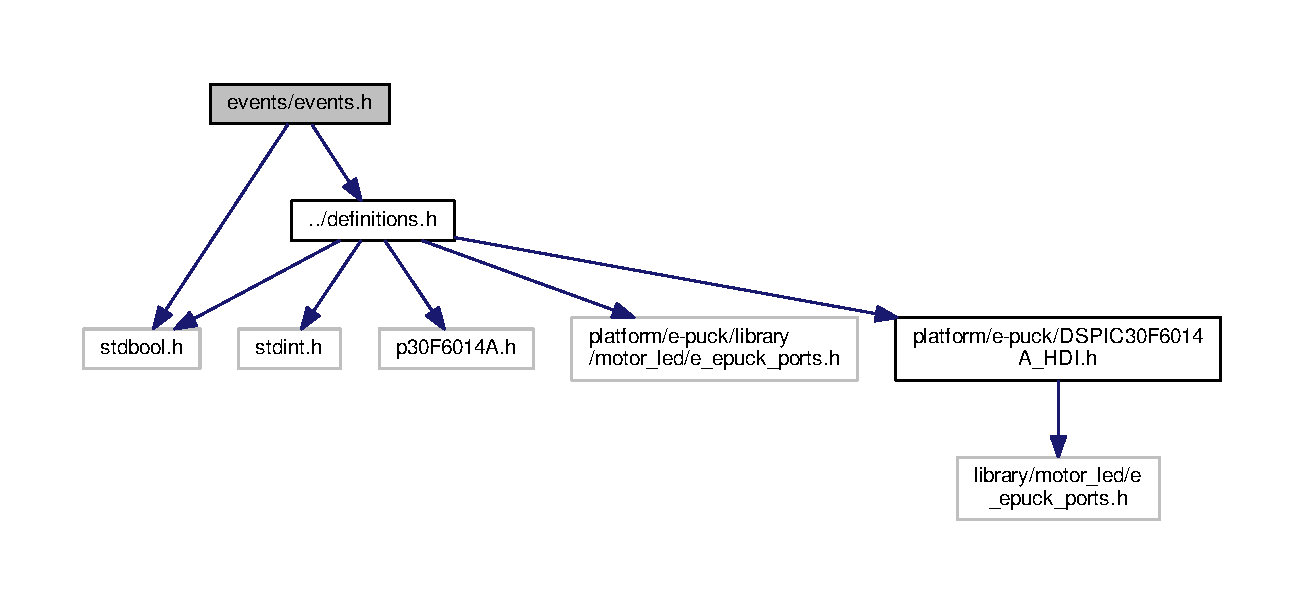
\includegraphics[width=350pt]{d4/dbb/events_8h__incl}
\end{center}
\end{figure}
This graph shows which files directly or indirectly include this file\+:\nopagebreak
\begin{figure}[H]
\begin{center}
\leavevmode
\includegraphics[width=350pt]{d2/d46/events_8h__dep__incl}
\end{center}
\end{figure}
\subsubsection*{Data Structures}
\begin{DoxyCompactItemize}
\item 
struct \hyperlink{structsys__event__data}{sys\+\_\+event\+\_\+data}
\begin{DoxyCompactList}\small\item\em It is a single linked list element and contains data of an occurred event. \end{DoxyCompactList}\end{DoxyCompactItemize}
\subsubsection*{Typedefs}
\begin{DoxyCompactItemize}
\item 
typedef bool($\ast$ \hyperlink{events_8h_a3db5730a7fed6827a4c46ff3fae3e55b}{p\+Event\+Handler\+Function}) (\hyperlink{definitions_8h_a1445ebbbf93d62972255ec5e89a5ab01}{uint}, \hyperlink{definitions_8h_a1445ebbbf93d62972255ec5e89a5ab01}{uint}, \hyperlink{structsys__event__data}{sys\+\_\+event\+\_\+data} $\ast$)
\begin{DoxyCompactList}\small\item\em Event handler function pointer type (process id, event id, received data) \end{DoxyCompactList}\item 
typedef bool($\ast$ \hyperlink{events_8h_a653a4a4b7d9f5a65e1415365267a9d9e}{p\+Condition\+Function}) (void $\ast$)
\begin{DoxyCompactList}\small\item\em Condition function pointer type. \end{DoxyCompactList}\end{DoxyCompactItemize}
\subsubsection*{Functions}
\begin{DoxyCompactItemize}
\item 
bool \hyperlink{events_8h_a67230a5307e77a8112e56436f372926f}{Sys\+\_\+\+Send\+\_\+\+Event} (\hyperlink{definitions_8h_a1445ebbbf93d62972255ec5e89a5ab01}{uint} event\+I\+D, void $\ast$data, \hyperlink{definitions_8h_a1445ebbbf93d62972255ec5e89a5ab01}{uint} data\+\_\+size)
\item 
bool \hyperlink{events_8h_a3b90448a001da0eee45d39ac8bb76ac0}{Sys\+\_\+\+Send\+\_\+\+Int\+Event} (\hyperlink{definitions_8h_a1445ebbbf93d62972255ec5e89a5ab01}{uint} event\+I\+D, \hyperlink{definitions_8h_a1445ebbbf93d62972255ec5e89a5ab01}{uint} data)
\item 
bool \hyperlink{events_8h_a5d9657772509ddb7ac6f6e1aa5730308}{Sys\+\_\+\+Register\+\_\+\+Event} (\hyperlink{definitions_8h_a1445ebbbf93d62972255ec5e89a5ab01}{uint} event\+I\+D)
\item 
void \hyperlink{events_8h_a41c81e9472691694352ac8316dc0ddbf}{Sys\+\_\+\+Unregister\+\_\+\+Event} (\hyperlink{definitions_8h_a1445ebbbf93d62972255ec5e89a5ab01}{uint} event\+I\+D)
\item 
bool \hyperlink{events_8h_a04afa9d5b243723e844d49ab9a7fd21e}{Sys\+\_\+\+Subscribe\+\_\+to\+\_\+\+Event} (\hyperlink{definitions_8h_a1445ebbbf93d62972255ec5e89a5ab01}{uint} event\+I\+D, \hyperlink{definitions_8h_a1445ebbbf93d62972255ec5e89a5ab01}{uint} pid, \hyperlink{events_8h_a3db5730a7fed6827a4c46ff3fae3e55b}{p\+Event\+Handler\+Function} handler, \hyperlink{events_8h_a653a4a4b7d9f5a65e1415365267a9d9e}{p\+Condition\+Function} condition)
\item 
void \hyperlink{events_8h_a267d472a623ac449be3922865e736029}{Sys\+\_\+\+Unsubscribe\+\_\+from\+\_\+\+Event} (\hyperlink{definitions_8h_a1445ebbbf93d62972255ec5e89a5ab01}{uint} event\+I\+D, \hyperlink{definitions_8h_a1445ebbbf93d62972255ec5e89a5ab01}{uint} pid)
\item 
void \hyperlink{events_8h_a71efab58004708fcd7e645ad10a213c1}{Sys\+\_\+\+Unsubscribe\+\_\+\+Process} (\hyperlink{definitions_8h_a1445ebbbf93d62972255ec5e89a5ab01}{uint} pid)
\item 
bool \hyperlink{events_8h_a9fc67102602189c4d1835c315719e368}{Sys\+\_\+\+Is\+Event\+Registered} (\hyperlink{definitions_8h_a1445ebbbf93d62972255ec5e89a5ab01}{uint} event\+I\+D)
\end{DoxyCompactItemize}


\subsubsection{Detailed Description}
declares functions to create, (un)subscribe, (un)register, and delete events and related handler. 

\begin{DoxyAuthor}{Author}
Stefan M. Trenkwalder \href{mailto:s.trenkwalder@openswarm.org}{\tt s.\+trenkwalder@openswarm.\+org} 
\end{DoxyAuthor}
\begin{DoxyVersion}{Version}
1.\+0
\end{DoxyVersion}
\begin{DoxyDate}{Date}
23 March 2015
\end{DoxyDate}
\begin{DoxyCopyright}{Copyright}
adapted Free\+B\+S\+D License (see \href{http://openswarm.org/license}{\tt http\+://openswarm.\+org/license}) 
\end{DoxyCopyright}


\subsubsection{Typedef Documentation}
\hypertarget{events_8h_a653a4a4b7d9f5a65e1415365267a9d9e}{}\index{events.\+h@{events.\+h}!p\+Condition\+Function@{p\+Condition\+Function}}
\index{p\+Condition\+Function@{p\+Condition\+Function}!events.\+h@{events.\+h}}
\paragraph[{p\+Condition\+Function}]{\setlength{\rightskip}{0pt plus 5cm}typedef bool($\ast$ p\+Condition\+Function) (void $\ast$)}\label{events_8h_a653a4a4b7d9f5a65e1415365267a9d9e}


Condition function pointer type. 

This function points to a condition function, which defines if an event handler should be executed or not. 

Definition at line 114 of file events.\+h.

\hypertarget{events_8h_a3db5730a7fed6827a4c46ff3fae3e55b}{}\index{events.\+h@{events.\+h}!p\+Event\+Handler\+Function@{p\+Event\+Handler\+Function}}
\index{p\+Event\+Handler\+Function@{p\+Event\+Handler\+Function}!events.\+h@{events.\+h}}
\paragraph[{p\+Event\+Handler\+Function}]{\setlength{\rightskip}{0pt plus 5cm}typedef bool($\ast$ p\+Event\+Handler\+Function) ({\bf uint}, {\bf uint}, {\bf sys\+\_\+event\+\_\+data} $\ast$)}\label{events_8h_a3db5730a7fed6827a4c46ff3fae3e55b}


Event handler function pointer type (process id, event id, received data) 

This function points to an event handler function, which processes incoming events and its data. 

Definition at line 107 of file events.\+h.



\subsubsection{Function Documentation}
\hypertarget{events_8h_a9fc67102602189c4d1835c315719e368}{}\index{events.\+h@{events.\+h}!Sys\+\_\+\+Is\+Event\+Registered@{Sys\+\_\+\+Is\+Event\+Registered}}
\index{Sys\+\_\+\+Is\+Event\+Registered@{Sys\+\_\+\+Is\+Event\+Registered}!events.\+h@{events.\+h}}
\paragraph[{Sys\+\_\+\+Is\+Event\+Registered}]{\setlength{\rightskip}{0pt plus 5cm}bool Sys\+\_\+\+Is\+Event\+Registered (
\begin{DoxyParamCaption}
\item[{{\bf uint}}]{event\+I\+D}
\end{DoxyParamCaption}
)}\label{events_8h_a9fc67102602189c4d1835c315719e368}
returns true if the event was registered


\begin{DoxyParams}[1]{Parameters}
\mbox{\tt in}  & {\em event\+I\+D} & I\+D of the event \\
\hline
\end{DoxyParams}
\begin{DoxyReturn}{Returns}
is the event registered? 
\end{DoxyReturn}


Definition at line 328 of file events.\+c.

\hypertarget{events_8h_a5d9657772509ddb7ac6f6e1aa5730308}{}\index{events.\+h@{events.\+h}!Sys\+\_\+\+Register\+\_\+\+Event@{Sys\+\_\+\+Register\+\_\+\+Event}}
\index{Sys\+\_\+\+Register\+\_\+\+Event@{Sys\+\_\+\+Register\+\_\+\+Event}!events.\+h@{events.\+h}}
\paragraph[{Sys\+\_\+\+Register\+\_\+\+Event}]{\setlength{\rightskip}{0pt plus 5cm}bool Sys\+\_\+\+Register\+\_\+\+Event (
\begin{DoxyParamCaption}
\item[{{\bf uint}}]{event\+I\+D}
\end{DoxyParamCaption}
)}\label{events_8h_a5d9657772509ddb7ac6f6e1aa5730308}
This function registers an new event. The registration tells the operating system that this event can occur.


\begin{DoxyParams}[1]{Parameters}
\mbox{\tt in}  & {\em event\+I\+D} & I\+D of the event \\
\hline
\end{DoxyParams}
\begin{DoxyReturn}{Returns}
was it successful. 
\end{DoxyReturn}


Definition at line 100 of file events.\+c.

\hypertarget{events_8h_a67230a5307e77a8112e56436f372926f}{}\index{events.\+h@{events.\+h}!Sys\+\_\+\+Send\+\_\+\+Event@{Sys\+\_\+\+Send\+\_\+\+Event}}
\index{Sys\+\_\+\+Send\+\_\+\+Event@{Sys\+\_\+\+Send\+\_\+\+Event}!events.\+h@{events.\+h}}
\paragraph[{Sys\+\_\+\+Send\+\_\+\+Event}]{\setlength{\rightskip}{0pt plus 5cm}bool Sys\+\_\+\+Send\+\_\+\+Event (
\begin{DoxyParamCaption}
\item[{{\bf uint}}]{event\+I\+D, }
\item[{void $\ast$}]{data, }
\item[{{\bf uint}}]{data\+\_\+size}
\end{DoxyParamCaption}
)}\label{events_8h_a67230a5307e77a8112e56436f372926f}
This function sends an event to all subscribers.


\begin{DoxyParams}[1]{Parameters}
\mbox{\tt in}  & {\em event\+I\+D} & I\+D of the event \\
\hline
\mbox{\tt in}  & {\em data} & pointer to the data that want to be sent as an event \\
\hline
\mbox{\tt in}  & {\em data\+\_\+size} & size of the data in bytes \\
\hline
\end{DoxyParams}
\begin{DoxyReturn}{Returns}
true if it was successful. 
\end{DoxyReturn}


Definition at line 61 of file events.\+c.

\hypertarget{events_8h_a3b90448a001da0eee45d39ac8bb76ac0}{}\index{events.\+h@{events.\+h}!Sys\+\_\+\+Send\+\_\+\+Int\+Event@{Sys\+\_\+\+Send\+\_\+\+Int\+Event}}
\index{Sys\+\_\+\+Send\+\_\+\+Int\+Event@{Sys\+\_\+\+Send\+\_\+\+Int\+Event}!events.\+h@{events.\+h}}
\paragraph[{Sys\+\_\+\+Send\+\_\+\+Int\+Event}]{\setlength{\rightskip}{0pt plus 5cm}bool Sys\+\_\+\+Send\+\_\+\+Int\+Event (
\begin{DoxyParamCaption}
\item[{{\bf uint}}]{event\+I\+D, }
\item[{{\bf uint}}]{data}
\end{DoxyParamCaption}
)\hspace{0.3cm}{\ttfamily [inline]}}\label{events_8h_a3b90448a001da0eee45d39ac8bb76ac0}
This function sends an integer (16-\/bit) to all subscribers.


\begin{DoxyParams}[1]{Parameters}
\mbox{\tt in}  & {\em event\+I\+D} & I\+D of the event \\
\hline
\mbox{\tt in}  & {\em data} & integer value that should be sent as an event \\
\hline
\end{DoxyParams}
\begin{DoxyReturn}{Returns}
was it successful. 
\end{DoxyReturn}


Definition at line 88 of file events.\+c.

\hypertarget{events_8h_a04afa9d5b243723e844d49ab9a7fd21e}{}\index{events.\+h@{events.\+h}!Sys\+\_\+\+Subscribe\+\_\+to\+\_\+\+Event@{Sys\+\_\+\+Subscribe\+\_\+to\+\_\+\+Event}}
\index{Sys\+\_\+\+Subscribe\+\_\+to\+\_\+\+Event@{Sys\+\_\+\+Subscribe\+\_\+to\+\_\+\+Event}!events.\+h@{events.\+h}}
\paragraph[{Sys\+\_\+\+Subscribe\+\_\+to\+\_\+\+Event}]{\setlength{\rightskip}{0pt plus 5cm}bool Sys\+\_\+\+Subscribe\+\_\+to\+\_\+\+Event (
\begin{DoxyParamCaption}
\item[{{\bf uint}}]{event\+I\+D, }
\item[{{\bf uint}}]{pid, }
\item[{{\bf p\+Event\+Handler\+Function}}]{handler, }
\item[{{\bf p\+Condition\+Function}}]{condition}
\end{DoxyParamCaption}
)}\label{events_8h_a04afa9d5b243723e844d49ab9a7fd21e}
This function subscribes a specific handler function to an process and a specific event


\begin{DoxyParams}[1]{Parameters}
\mbox{\tt in}  & {\em event\+I\+D} & I\+D of the event \\
\hline
\mbox{\tt in}  & {\em pid} & I\+D of the process \\
\hline
\mbox{\tt in}  & {\em handler} & pointer to the function that should handle the event data \\
\hline
\mbox{\tt in}  & {\em condition} & pointer to the function that decides if the handler should be executed or not \\
\hline
\end{DoxyParams}
\begin{DoxyReturn}{Returns}
was it successful. 
\end{DoxyReturn}


Definition at line 142 of file events.\+c.

\hypertarget{events_8h_a41c81e9472691694352ac8316dc0ddbf}{}\index{events.\+h@{events.\+h}!Sys\+\_\+\+Unregister\+\_\+\+Event@{Sys\+\_\+\+Unregister\+\_\+\+Event}}
\index{Sys\+\_\+\+Unregister\+\_\+\+Event@{Sys\+\_\+\+Unregister\+\_\+\+Event}!events.\+h@{events.\+h}}
\paragraph[{Sys\+\_\+\+Unregister\+\_\+\+Event}]{\setlength{\rightskip}{0pt plus 5cm}void Sys\+\_\+\+Unregister\+\_\+\+Event (
\begin{DoxyParamCaption}
\item[{{\bf uint}}]{event\+I\+D}
\end{DoxyParamCaption}
)}\label{events_8h_a41c81e9472691694352ac8316dc0ddbf}
This function unregisters an event


\begin{DoxyParams}[1]{Parameters}
\mbox{\tt in}  & {\em event\+I\+D} & I\+D of the event \\
\hline
\end{DoxyParams}


Definition at line 187 of file events.\+c.

\hypertarget{events_8h_a267d472a623ac449be3922865e736029}{}\index{events.\+h@{events.\+h}!Sys\+\_\+\+Unsubscribe\+\_\+from\+\_\+\+Event@{Sys\+\_\+\+Unsubscribe\+\_\+from\+\_\+\+Event}}
\index{Sys\+\_\+\+Unsubscribe\+\_\+from\+\_\+\+Event@{Sys\+\_\+\+Unsubscribe\+\_\+from\+\_\+\+Event}!events.\+h@{events.\+h}}
\paragraph[{Sys\+\_\+\+Unsubscribe\+\_\+from\+\_\+\+Event}]{\setlength{\rightskip}{0pt plus 5cm}void Sys\+\_\+\+Unsubscribe\+\_\+from\+\_\+\+Event (
\begin{DoxyParamCaption}
\item[{{\bf uint}}]{event\+I\+D, }
\item[{{\bf uint}}]{pid}
\end{DoxyParamCaption}
)}\label{events_8h_a267d472a623ac449be3922865e736029}
This function unsubscribes an event


\begin{DoxyParams}[1]{Parameters}
\mbox{\tt in}  & {\em event\+I\+D} & I\+D of the event \\
\hline
\mbox{\tt in}  & {\em pid} & I\+D of the process \\
\hline
\end{DoxyParams}


Definition at line 238 of file events.\+c.

\hypertarget{events_8h_a71efab58004708fcd7e645ad10a213c1}{}\index{events.\+h@{events.\+h}!Sys\+\_\+\+Unsubscribe\+\_\+\+Process@{Sys\+\_\+\+Unsubscribe\+\_\+\+Process}}
\index{Sys\+\_\+\+Unsubscribe\+\_\+\+Process@{Sys\+\_\+\+Unsubscribe\+\_\+\+Process}!events.\+h@{events.\+h}}
\paragraph[{Sys\+\_\+\+Unsubscribe\+\_\+\+Process}]{\setlength{\rightskip}{0pt plus 5cm}void Sys\+\_\+\+Unsubscribe\+\_\+\+Process (
\begin{DoxyParamCaption}
\item[{{\bf uint}}]{pid}
\end{DoxyParamCaption}
)}\label{events_8h_a71efab58004708fcd7e645ad10a213c1}
unsubscribes all events that were subscribed to a process


\begin{DoxyParams}[1]{Parameters}
\mbox{\tt in}  & {\em pid} & process identifier \\
\hline
\end{DoxyParams}


Definition at line 347 of file events.\+c.


\hypertarget{interrupts_8c}{}\section{interrupts.\+c File Reference}
\label{interrupts_8c}\index{interrupts.\+c@{interrupts.\+c}}


It defines the functions to create atomic sections.  


{\ttfamily \#include \char`\"{}interrupts.\+h\char`\"{}}\\*
{\ttfamily \#include \char`\"{}definitions.\+h\char`\"{}}\\*
Include dependency graph for interrupts.\+c\+:
\nopagebreak
\begin{figure}[H]
\begin{center}
\leavevmode
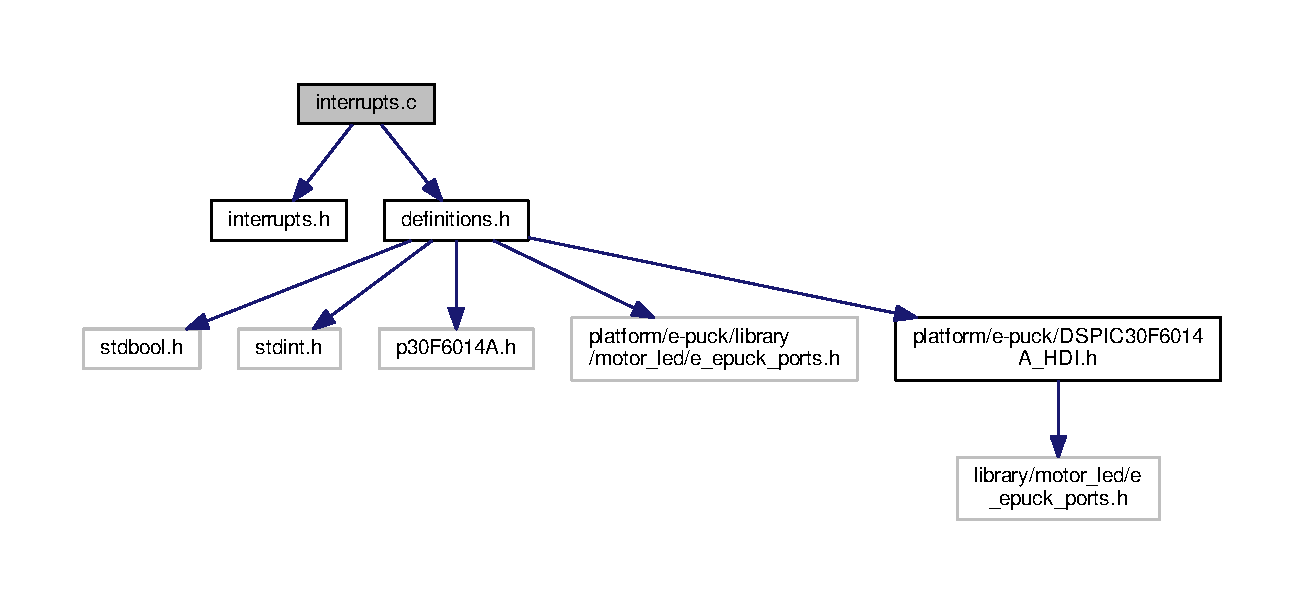
\includegraphics[width=350pt]{d3/d24/interrupts_8c__incl}
\end{center}
\end{figure}
\subsection*{Functions}
\begin{DoxyCompactItemize}
\item 
void \hyperlink{interrupts_8c_acce68565a1263b2b7bc870bfe0601f45}{Sys\+\_\+\+Start\+\_\+\+Atomic\+Section} ()
\item 
void \hyperlink{interrupts_8c_a04cce7e66e6b181477698c6398714240}{Sys\+\_\+\+End\+\_\+\+Atomic\+Section} ()
\end{DoxyCompactItemize}


\subsection{Detailed Description}
It defines the functions to create atomic sections. 

\begin{DoxyAuthor}{Author}
Stefan M. Trenkwalder \href{mailto:s.trenkwalder@openswarm.org}{\tt s.\+trenkwalder@openswarm.\+org} 
\end{DoxyAuthor}
\begin{DoxyVersion}{Version}
1.\+0 
\end{DoxyVersion}
\begin{DoxyDate}{Date}
2015 
\end{DoxyDate}
\begin{DoxyCopyright}{Copyright}
adapted Free\+B\+S\+D License (see \href{http://openswarm.org/license}{\tt http\+://openswarm.\+org/license})
\end{DoxyCopyright}
~\newline
 To protect sections of code from any interruptions one has to use the following code\+: 
\begin{DoxyCode}
\textcolor{comment}{// do something}

\hyperlink{interrupts_8c_acce68565a1263b2b7bc870bfe0601f45}{Sys\_Start\_AtomicSection}();
     
     \textcolor{comment}{//do something which should not be interrupted     }

\hyperlink{interrupts_8c_a04cce7e66e6b181477698c6398714240}{Sys\_End\_AtomicSection}();

\textcolor{comment}{// do something else}
\end{DoxyCode}
 

\subsection{Function Documentation}
\hypertarget{interrupts_8c_a04cce7e66e6b181477698c6398714240}{}\index{interrupts.\+c@{interrupts.\+c}!Sys\+\_\+\+End\+\_\+\+Atomic\+Section@{Sys\+\_\+\+End\+\_\+\+Atomic\+Section}}
\index{Sys\+\_\+\+End\+\_\+\+Atomic\+Section@{Sys\+\_\+\+End\+\_\+\+Atomic\+Section}!interrupts.\+c@{interrupts.\+c}}
\subsubsection[{Sys\+\_\+\+End\+\_\+\+Atomic\+Section}]{\setlength{\rightskip}{0pt plus 5cm}void Sys\+\_\+\+End\+\_\+\+Atomic\+Section (
\begin{DoxyParamCaption}
\item[{void}]{}
\end{DoxyParamCaption}
)\hspace{0.3cm}{\ttfamily [inline]}}\label{interrupts_8c_a04cce7e66e6b181477698c6398714240}
Starts an atomic section

This Function starts an atomic section. This means the code afterwards cannot be interrupted by any interrupt. \begin{DoxyPrecond}{Precondition}
\hyperlink{interrupts_8c_acce68565a1263b2b7bc870bfe0601f45}{Sys\+\_\+\+Start\+\_\+\+Atomic\+Section()} must have been called. 
\end{DoxyPrecond}


Definition at line 58 of file interrupts.\+c.

\hypertarget{interrupts_8c_acce68565a1263b2b7bc870bfe0601f45}{}\index{interrupts.\+c@{interrupts.\+c}!Sys\+\_\+\+Start\+\_\+\+Atomic\+Section@{Sys\+\_\+\+Start\+\_\+\+Atomic\+Section}}
\index{Sys\+\_\+\+Start\+\_\+\+Atomic\+Section@{Sys\+\_\+\+Start\+\_\+\+Atomic\+Section}!interrupts.\+c@{interrupts.\+c}}
\subsubsection[{Sys\+\_\+\+Start\+\_\+\+Atomic\+Section}]{\setlength{\rightskip}{0pt plus 5cm}void Sys\+\_\+\+Start\+\_\+\+Atomic\+Section (
\begin{DoxyParamCaption}
\item[{void}]{}
\end{DoxyParamCaption}
)\hspace{0.3cm}{\ttfamily [inline]}}\label{interrupts_8c_acce68565a1263b2b7bc870bfe0601f45}
Starts an atomic section

This Function starts an atomic section. This means the code afterwards cannot be interrupted by any interrupt. \begin{DoxyNote}{Note}
This function can be called within an atomic section. However, it doesn\textquotesingle{}t change the behaviour when called within an atomic section. To end an atomic section, \hyperlink{interrupts_8c_a04cce7e66e6b181477698c6398714240}{Sys\+\_\+\+End\+\_\+\+Atomic\+Section()} must be called as often as \hyperlink{interrupts_8c_acce68565a1263b2b7bc870bfe0601f45}{Sys\+\_\+\+Start\+\_\+\+Atomic\+Section()} was called. 
\end{DoxyNote}
\begin{DoxyPostcond}{Postcondition}
\hyperlink{interrupts_8c_a04cce7e66e6b181477698c6398714240}{Sys\+\_\+\+End\+\_\+\+Atomic\+Section()} must be called to execute any interrupt that happened or will happen. 
\end{DoxyPostcond}


Definition at line 43 of file interrupts.\+c.


\hypertarget{interrupts_8h}{}\section{interrupts.\+h File Reference}
\label{interrupts_8h}\index{interrupts.\+h@{interrupts.\+h}}


It declares interrupt priority levels and functions to create atomic sections.  


This graph shows which files directly or indirectly include this file\+:
\nopagebreak
\begin{figure}[H]
\begin{center}
\leavevmode
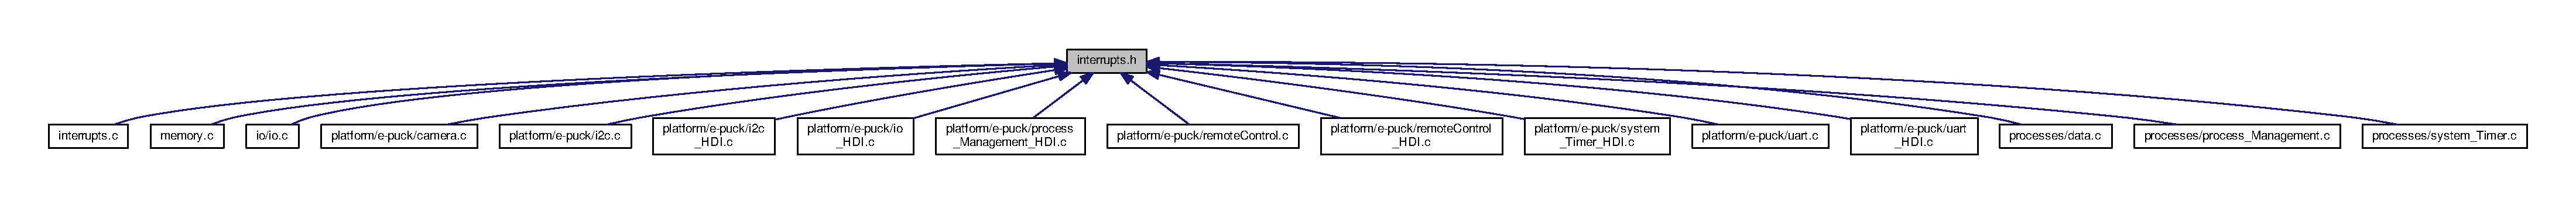
\includegraphics[width=350pt]{d9/d4e/interrupts_8h__dep__incl}
\end{center}
\end{figure}
\subsection*{Macros}
\begin{DoxyCompactItemize}
\item 
\#define \hyperlink{interrupts_8h_a2665dac9b4f047c8d82e7076eb2c1f0b}{S\+Y\+S\+\_\+\+I\+R\+Q\+P\+\_\+\+M\+A\+X}~7
\item 
\#define \hyperlink{interrupts_8h_ae792a67469dbfd96699107868d70b89d}{S\+Y\+S\+\_\+\+I\+R\+Q\+P\+\_\+\+S\+Y\+S\+T\+E\+M\+\_\+\+T\+I\+M\+E\+R}~2
\item 
\#define \hyperlink{interrupts_8h_acea06e741c8e65e966768399b39550fd}{S\+Y\+S\+\_\+\+I\+R\+Q\+P\+\_\+\+I\+O\+\_\+\+T\+I\+M\+E\+R}~3
\item 
\#define \hyperlink{interrupts_8h_a20e8d0849325b72878dc32b27876a07b}{S\+Y\+S\+\_\+\+I\+R\+Q\+P\+\_\+\+U\+A\+R\+T1}~4
\item 
\#define \hyperlink{interrupts_8h_a8a1e0a0bb08cf252f8ffe0d80f04cf49}{S\+Y\+S\+\_\+\+I\+R\+Q\+P\+\_\+\+U\+A\+R\+T2}~4
\item 
\#define \hyperlink{interrupts_8h_abe88b597dc055319b1224b2bfda0ed78}{S\+Y\+S\+\_\+\+I\+R\+Q\+P\+\_\+\+I2\+C}~5
\item 
\#define \hyperlink{interrupts_8h_a8861626b5e152d2faca2df0622c0d48e}{S\+Y\+S\+\_\+\+I\+R\+Q\+P\+\_\+\+R\+E\+M\+O\+T\+E\+C\+O\+N\+T\+R\+O\+L}~4
\item 
\#define \hyperlink{interrupts_8h_a325ecca3d1e3afcb63ac4c6170f8187c}{S\+Y\+S\+\_\+\+I\+R\+Q\+P\+\_\+\+C\+A\+M\+E\+R\+A\+\_\+\+P\+I\+X\+E\+L}~5
\item 
\#define \hyperlink{interrupts_8h_ad7c4deb027ed01f91a2fa272bb8b7b18}{S\+Y\+S\+\_\+\+I\+R\+Q\+P\+\_\+\+C\+A\+M\+E\+R\+A\+\_\+\+L\+I\+N\+E}~6
\item 
\#define \hyperlink{interrupts_8h_a14f55cc62d9f3cca0bd84c72c5415cfc}{S\+Y\+S\+\_\+\+I\+R\+Q\+P\+\_\+\+C\+A\+M\+E\+R\+A\+\_\+\+F\+R\+A\+M\+E}~7
\end{DoxyCompactItemize}
\subsection*{Functions}
\begin{DoxyCompactItemize}
\item 
void \hyperlink{interrupts_8h_abf5948c864c1ddce2f7b4a4624f6006f}{Sys\+\_\+\+Start\+\_\+\+Atomic\+Section} (void)
\item 
void \hyperlink{interrupts_8h_aec2c903ebd9339ced317b3a9df5f8433}{Sys\+\_\+\+End\+\_\+\+Atomic\+Section} (void)
\end{DoxyCompactItemize}


\subsection{Detailed Description}
It declares interrupt priority levels and functions to create atomic sections. 

\begin{DoxyAuthor}{Author}
Stefan M. Trenkwalder \href{mailto:s.trenkwalder@openswarm.org}{\tt s.\+trenkwalder@openswarm.\+org} 
\end{DoxyAuthor}
\begin{DoxyVersion}{Version}
1.\+0
\end{DoxyVersion}
\begin{DoxyDate}{Date}
\{03 September 2015\}
\end{DoxyDate}
\begin{DoxyCopyright}{Copyright}
adapted Free\+B\+S\+D License (see \href{http://openswarm.org/license}{\tt http\+://openswarm.\+org/license}) 
\end{DoxyCopyright}


\subsection{Macro Definition Documentation}
\hypertarget{interrupts_8h_a14f55cc62d9f3cca0bd84c72c5415cfc}{}\index{interrupts.\+h@{interrupts.\+h}!S\+Y\+S\+\_\+\+I\+R\+Q\+P\+\_\+\+C\+A\+M\+E\+R\+A\+\_\+\+F\+R\+A\+M\+E@{S\+Y\+S\+\_\+\+I\+R\+Q\+P\+\_\+\+C\+A\+M\+E\+R\+A\+\_\+\+F\+R\+A\+M\+E}}
\index{S\+Y\+S\+\_\+\+I\+R\+Q\+P\+\_\+\+C\+A\+M\+E\+R\+A\+\_\+\+F\+R\+A\+M\+E@{S\+Y\+S\+\_\+\+I\+R\+Q\+P\+\_\+\+C\+A\+M\+E\+R\+A\+\_\+\+F\+R\+A\+M\+E}!interrupts.\+h@{interrupts.\+h}}
\subsubsection[{S\+Y\+S\+\_\+\+I\+R\+Q\+P\+\_\+\+C\+A\+M\+E\+R\+A\+\_\+\+F\+R\+A\+M\+E}]{\setlength{\rightskip}{0pt plus 5cm}\#define S\+Y\+S\+\_\+\+I\+R\+Q\+P\+\_\+\+C\+A\+M\+E\+R\+A\+\_\+\+F\+R\+A\+M\+E~7}\label{interrupts_8h_a14f55cc62d9f3cca0bd84c72c5415cfc}
interrupt priority for the camera frame interrupt 

Definition at line 35 of file interrupts.\+h.

\hypertarget{interrupts_8h_ad7c4deb027ed01f91a2fa272bb8b7b18}{}\index{interrupts.\+h@{interrupts.\+h}!S\+Y\+S\+\_\+\+I\+R\+Q\+P\+\_\+\+C\+A\+M\+E\+R\+A\+\_\+\+L\+I\+N\+E@{S\+Y\+S\+\_\+\+I\+R\+Q\+P\+\_\+\+C\+A\+M\+E\+R\+A\+\_\+\+L\+I\+N\+E}}
\index{S\+Y\+S\+\_\+\+I\+R\+Q\+P\+\_\+\+C\+A\+M\+E\+R\+A\+\_\+\+L\+I\+N\+E@{S\+Y\+S\+\_\+\+I\+R\+Q\+P\+\_\+\+C\+A\+M\+E\+R\+A\+\_\+\+L\+I\+N\+E}!interrupts.\+h@{interrupts.\+h}}
\subsubsection[{S\+Y\+S\+\_\+\+I\+R\+Q\+P\+\_\+\+C\+A\+M\+E\+R\+A\+\_\+\+L\+I\+N\+E}]{\setlength{\rightskip}{0pt plus 5cm}\#define S\+Y\+S\+\_\+\+I\+R\+Q\+P\+\_\+\+C\+A\+M\+E\+R\+A\+\_\+\+L\+I\+N\+E~6}\label{interrupts_8h_ad7c4deb027ed01f91a2fa272bb8b7b18}
interrupt priority for the camera line interrupt 

Definition at line 34 of file interrupts.\+h.

\hypertarget{interrupts_8h_a325ecca3d1e3afcb63ac4c6170f8187c}{}\index{interrupts.\+h@{interrupts.\+h}!S\+Y\+S\+\_\+\+I\+R\+Q\+P\+\_\+\+C\+A\+M\+E\+R\+A\+\_\+\+P\+I\+X\+E\+L@{S\+Y\+S\+\_\+\+I\+R\+Q\+P\+\_\+\+C\+A\+M\+E\+R\+A\+\_\+\+P\+I\+X\+E\+L}}
\index{S\+Y\+S\+\_\+\+I\+R\+Q\+P\+\_\+\+C\+A\+M\+E\+R\+A\+\_\+\+P\+I\+X\+E\+L@{S\+Y\+S\+\_\+\+I\+R\+Q\+P\+\_\+\+C\+A\+M\+E\+R\+A\+\_\+\+P\+I\+X\+E\+L}!interrupts.\+h@{interrupts.\+h}}
\subsubsection[{S\+Y\+S\+\_\+\+I\+R\+Q\+P\+\_\+\+C\+A\+M\+E\+R\+A\+\_\+\+P\+I\+X\+E\+L}]{\setlength{\rightskip}{0pt plus 5cm}\#define S\+Y\+S\+\_\+\+I\+R\+Q\+P\+\_\+\+C\+A\+M\+E\+R\+A\+\_\+\+P\+I\+X\+E\+L~5}\label{interrupts_8h_a325ecca3d1e3afcb63ac4c6170f8187c}
interrupt priority for the camera pixel interrupt 

Definition at line 33 of file interrupts.\+h.

\hypertarget{interrupts_8h_abe88b597dc055319b1224b2bfda0ed78}{}\index{interrupts.\+h@{interrupts.\+h}!S\+Y\+S\+\_\+\+I\+R\+Q\+P\+\_\+\+I2\+C@{S\+Y\+S\+\_\+\+I\+R\+Q\+P\+\_\+\+I2\+C}}
\index{S\+Y\+S\+\_\+\+I\+R\+Q\+P\+\_\+\+I2\+C@{S\+Y\+S\+\_\+\+I\+R\+Q\+P\+\_\+\+I2\+C}!interrupts.\+h@{interrupts.\+h}}
\subsubsection[{S\+Y\+S\+\_\+\+I\+R\+Q\+P\+\_\+\+I2\+C}]{\setlength{\rightskip}{0pt plus 5cm}\#define S\+Y\+S\+\_\+\+I\+R\+Q\+P\+\_\+\+I2\+C~5}\label{interrupts_8h_abe88b597dc055319b1224b2bfda0ed78}
interrupt priority for the I2\+C interrupt 

Definition at line 29 of file interrupts.\+h.

\hypertarget{interrupts_8h_acea06e741c8e65e966768399b39550fd}{}\index{interrupts.\+h@{interrupts.\+h}!S\+Y\+S\+\_\+\+I\+R\+Q\+P\+\_\+\+I\+O\+\_\+\+T\+I\+M\+E\+R@{S\+Y\+S\+\_\+\+I\+R\+Q\+P\+\_\+\+I\+O\+\_\+\+T\+I\+M\+E\+R}}
\index{S\+Y\+S\+\_\+\+I\+R\+Q\+P\+\_\+\+I\+O\+\_\+\+T\+I\+M\+E\+R@{S\+Y\+S\+\_\+\+I\+R\+Q\+P\+\_\+\+I\+O\+\_\+\+T\+I\+M\+E\+R}!interrupts.\+h@{interrupts.\+h}}
\subsubsection[{S\+Y\+S\+\_\+\+I\+R\+Q\+P\+\_\+\+I\+O\+\_\+\+T\+I\+M\+E\+R}]{\setlength{\rightskip}{0pt plus 5cm}\#define S\+Y\+S\+\_\+\+I\+R\+Q\+P\+\_\+\+I\+O\+\_\+\+T\+I\+M\+E\+R~3}\label{interrupts_8h_acea06e741c8e65e966768399b39550fd}
interrupt priority for the I/\+O timer interrupt 

Definition at line 24 of file interrupts.\+h.

\hypertarget{interrupts_8h_a2665dac9b4f047c8d82e7076eb2c1f0b}{}\index{interrupts.\+h@{interrupts.\+h}!S\+Y\+S\+\_\+\+I\+R\+Q\+P\+\_\+\+M\+A\+X@{S\+Y\+S\+\_\+\+I\+R\+Q\+P\+\_\+\+M\+A\+X}}
\index{S\+Y\+S\+\_\+\+I\+R\+Q\+P\+\_\+\+M\+A\+X@{S\+Y\+S\+\_\+\+I\+R\+Q\+P\+\_\+\+M\+A\+X}!interrupts.\+h@{interrupts.\+h}}
\subsubsection[{S\+Y\+S\+\_\+\+I\+R\+Q\+P\+\_\+\+M\+A\+X}]{\setlength{\rightskip}{0pt plus 5cm}\#define S\+Y\+S\+\_\+\+I\+R\+Q\+P\+\_\+\+M\+A\+X~7}\label{interrupts_8h_a2665dac9b4f047c8d82e7076eb2c1f0b}
maximum interrupt priority 

Definition at line 20 of file interrupts.\+h.

\hypertarget{interrupts_8h_a8861626b5e152d2faca2df0622c0d48e}{}\index{interrupts.\+h@{interrupts.\+h}!S\+Y\+S\+\_\+\+I\+R\+Q\+P\+\_\+\+R\+E\+M\+O\+T\+E\+C\+O\+N\+T\+R\+O\+L@{S\+Y\+S\+\_\+\+I\+R\+Q\+P\+\_\+\+R\+E\+M\+O\+T\+E\+C\+O\+N\+T\+R\+O\+L}}
\index{S\+Y\+S\+\_\+\+I\+R\+Q\+P\+\_\+\+R\+E\+M\+O\+T\+E\+C\+O\+N\+T\+R\+O\+L@{S\+Y\+S\+\_\+\+I\+R\+Q\+P\+\_\+\+R\+E\+M\+O\+T\+E\+C\+O\+N\+T\+R\+O\+L}!interrupts.\+h@{interrupts.\+h}}
\subsubsection[{S\+Y\+S\+\_\+\+I\+R\+Q\+P\+\_\+\+R\+E\+M\+O\+T\+E\+C\+O\+N\+T\+R\+O\+L}]{\setlength{\rightskip}{0pt plus 5cm}\#define S\+Y\+S\+\_\+\+I\+R\+Q\+P\+\_\+\+R\+E\+M\+O\+T\+E\+C\+O\+N\+T\+R\+O\+L~4}\label{interrupts_8h_a8861626b5e152d2faca2df0622c0d48e}
interrupt priority for the remote control interrupt 

Definition at line 31 of file interrupts.\+h.

\hypertarget{interrupts_8h_ae792a67469dbfd96699107868d70b89d}{}\index{interrupts.\+h@{interrupts.\+h}!S\+Y\+S\+\_\+\+I\+R\+Q\+P\+\_\+\+S\+Y\+S\+T\+E\+M\+\_\+\+T\+I\+M\+E\+R@{S\+Y\+S\+\_\+\+I\+R\+Q\+P\+\_\+\+S\+Y\+S\+T\+E\+M\+\_\+\+T\+I\+M\+E\+R}}
\index{S\+Y\+S\+\_\+\+I\+R\+Q\+P\+\_\+\+S\+Y\+S\+T\+E\+M\+\_\+\+T\+I\+M\+E\+R@{S\+Y\+S\+\_\+\+I\+R\+Q\+P\+\_\+\+S\+Y\+S\+T\+E\+M\+\_\+\+T\+I\+M\+E\+R}!interrupts.\+h@{interrupts.\+h}}
\subsubsection[{S\+Y\+S\+\_\+\+I\+R\+Q\+P\+\_\+\+S\+Y\+S\+T\+E\+M\+\_\+\+T\+I\+M\+E\+R}]{\setlength{\rightskip}{0pt plus 5cm}\#define S\+Y\+S\+\_\+\+I\+R\+Q\+P\+\_\+\+S\+Y\+S\+T\+E\+M\+\_\+\+T\+I\+M\+E\+R~2}\label{interrupts_8h_ae792a67469dbfd96699107868d70b89d}
interrupt priority for the system timer interrupt 

Definition at line 22 of file interrupts.\+h.

\hypertarget{interrupts_8h_a20e8d0849325b72878dc32b27876a07b}{}\index{interrupts.\+h@{interrupts.\+h}!S\+Y\+S\+\_\+\+I\+R\+Q\+P\+\_\+\+U\+A\+R\+T1@{S\+Y\+S\+\_\+\+I\+R\+Q\+P\+\_\+\+U\+A\+R\+T1}}
\index{S\+Y\+S\+\_\+\+I\+R\+Q\+P\+\_\+\+U\+A\+R\+T1@{S\+Y\+S\+\_\+\+I\+R\+Q\+P\+\_\+\+U\+A\+R\+T1}!interrupts.\+h@{interrupts.\+h}}
\subsubsection[{S\+Y\+S\+\_\+\+I\+R\+Q\+P\+\_\+\+U\+A\+R\+T1}]{\setlength{\rightskip}{0pt plus 5cm}\#define S\+Y\+S\+\_\+\+I\+R\+Q\+P\+\_\+\+U\+A\+R\+T1~4}\label{interrupts_8h_a20e8d0849325b72878dc32b27876a07b}
interrupt priority for the U\+A\+R\+T1 interrupt 

Definition at line 26 of file interrupts.\+h.

\hypertarget{interrupts_8h_a8a1e0a0bb08cf252f8ffe0d80f04cf49}{}\index{interrupts.\+h@{interrupts.\+h}!S\+Y\+S\+\_\+\+I\+R\+Q\+P\+\_\+\+U\+A\+R\+T2@{S\+Y\+S\+\_\+\+I\+R\+Q\+P\+\_\+\+U\+A\+R\+T2}}
\index{S\+Y\+S\+\_\+\+I\+R\+Q\+P\+\_\+\+U\+A\+R\+T2@{S\+Y\+S\+\_\+\+I\+R\+Q\+P\+\_\+\+U\+A\+R\+T2}!interrupts.\+h@{interrupts.\+h}}
\subsubsection[{S\+Y\+S\+\_\+\+I\+R\+Q\+P\+\_\+\+U\+A\+R\+T2}]{\setlength{\rightskip}{0pt plus 5cm}\#define S\+Y\+S\+\_\+\+I\+R\+Q\+P\+\_\+\+U\+A\+R\+T2~4}\label{interrupts_8h_a8a1e0a0bb08cf252f8ffe0d80f04cf49}
interrupt priority for the U\+A\+R\+T2 interrupt 

Definition at line 27 of file interrupts.\+h.



\subsection{Function Documentation}
\hypertarget{interrupts_8h_aec2c903ebd9339ced317b3a9df5f8433}{}\index{interrupts.\+h@{interrupts.\+h}!Sys\+\_\+\+End\+\_\+\+Atomic\+Section@{Sys\+\_\+\+End\+\_\+\+Atomic\+Section}}
\index{Sys\+\_\+\+End\+\_\+\+Atomic\+Section@{Sys\+\_\+\+End\+\_\+\+Atomic\+Section}!interrupts.\+h@{interrupts.\+h}}
\subsubsection[{Sys\+\_\+\+End\+\_\+\+Atomic\+Section}]{\setlength{\rightskip}{0pt plus 5cm}void Sys\+\_\+\+End\+\_\+\+Atomic\+Section (
\begin{DoxyParamCaption}
\item[{void}]{}
\end{DoxyParamCaption}
)\hspace{0.3cm}{\ttfamily [inline]}}\label{interrupts_8h_aec2c903ebd9339ced317b3a9df5f8433}
Starts an atomic section

This Function starts an atomic section. This means the code afterwards cannot be interrupted by any interrupt. \begin{DoxyPrecond}{Precondition}
\hyperlink{interrupts_8c_acce68565a1263b2b7bc870bfe0601f45}{Sys\+\_\+\+Start\+\_\+\+Atomic\+Section()} must have been called. 
\end{DoxyPrecond}


Definition at line 58 of file interrupts.\+c.

\hypertarget{interrupts_8h_abf5948c864c1ddce2f7b4a4624f6006f}{}\index{interrupts.\+h@{interrupts.\+h}!Sys\+\_\+\+Start\+\_\+\+Atomic\+Section@{Sys\+\_\+\+Start\+\_\+\+Atomic\+Section}}
\index{Sys\+\_\+\+Start\+\_\+\+Atomic\+Section@{Sys\+\_\+\+Start\+\_\+\+Atomic\+Section}!interrupts.\+h@{interrupts.\+h}}
\subsubsection[{Sys\+\_\+\+Start\+\_\+\+Atomic\+Section}]{\setlength{\rightskip}{0pt plus 5cm}void Sys\+\_\+\+Start\+\_\+\+Atomic\+Section (
\begin{DoxyParamCaption}
\item[{void}]{}
\end{DoxyParamCaption}
)\hspace{0.3cm}{\ttfamily [inline]}}\label{interrupts_8h_abf5948c864c1ddce2f7b4a4624f6006f}
Starts an atomic section

This Function starts an atomic section. This means the code afterwards cannot be interrupted by any interrupt. \begin{DoxyNote}{Note}
This function can be called within an atomic section. However, it doesn\textquotesingle{}t change the behaviour when called within an atomic section. To end an atomic section, \hyperlink{interrupts_8c_a04cce7e66e6b181477698c6398714240}{Sys\+\_\+\+End\+\_\+\+Atomic\+Section()} must be called as often as \hyperlink{interrupts_8c_acce68565a1263b2b7bc870bfe0601f45}{Sys\+\_\+\+Start\+\_\+\+Atomic\+Section()} was called. 
\end{DoxyNote}
\begin{DoxyPostcond}{Postcondition}
\hyperlink{interrupts_8c_a04cce7e66e6b181477698c6398714240}{Sys\+\_\+\+End\+\_\+\+Atomic\+Section()} must be called to execute any interrupt that happened or will happen. 
\end{DoxyPostcond}


Definition at line 43 of file interrupts.\+c.


\hypertarget{io_8c}{}\section{io/io.c File Reference}
\label{io_8c}\index{io/io.\+c@{io/io.\+c}}


This file includes the I\+O timer to start and stop the timer. This timer executes I\+O functions periodically.  


{\ttfamily \#include \char`\"{}io.\+h\char`\"{}}\\*
{\ttfamily \#include \char`\"{}../definitions.\+h\char`\"{}}\\*
{\ttfamily \#include \char`\"{}e-\/puck/io\+\_\+\+H\+D\+I.\+h\char`\"{}}\\*
{\ttfamily \#include \char`\"{}../interrupts.\+h\char`\"{}}\\*
{\ttfamily \#include \char`\"{}../memory.\+h\char`\"{}}\\*
Include dependency graph for io.\+c\+:\nopagebreak
\begin{figure}[H]
\begin{center}
\leavevmode
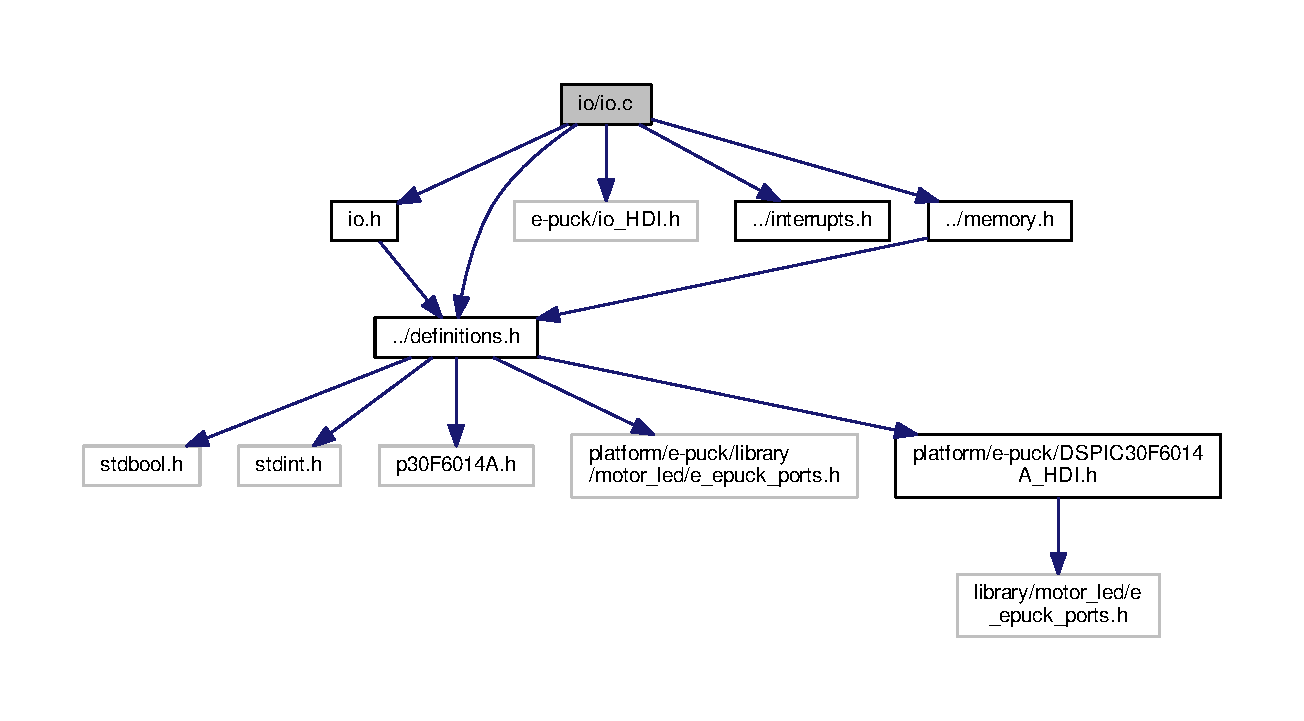
\includegraphics[width=350pt]{d3/d43/io_8c__incl}
\end{center}
\end{figure}
\subsection*{Functions}
\begin{DoxyCompactItemize}
\item 
void \hyperlink{io_8c_ad1719208a5855f34e056a8114de973f9}{Sys\+\_\+\+Init\+\_\+\+I\+O\+Management} (void)
\item 
void \hyperlink{io_8c_a6ca66df90d159586d58a19e01f3a7025}{Sys\+\_\+\+Start\+\_\+\+I\+O\+Management} (void)
\item 
void \hyperlink{io_8c_a14d9a8f941c03184049f3bf18d35fb47}{Sys\+\_\+\+Stop\+\_\+\+I\+O\+Management} (void)
\item 
void \hyperlink{io_8c_aa0fae8c15b4399acf3605e6628e8ec23}{Sys\+\_\+\+Stop\+\_\+\+I\+O\+Timer} ()
\item 
void \hyperlink{io_8c_a9a2914a7c7a18f6edcbb223156854562}{Sys\+\_\+\+Continue\+\_\+\+I\+O\+Timer} ()
\item 
void \hyperlink{io_8c_a4539e84ae7a33de9927b19e7ce59285e}{Sys\+\_\+\+Reset\+\_\+\+I\+O\+Timer} ()
\item 
void \hyperlink{io_8c_ac0b26f07f393a09d948530299ac39c9d}{Sys\+\_\+\+Disable\+\_\+\+I\+O\+Timer\+Interrupt} ()
\item 
void \hyperlink{io_8c_afdcf87dbfc3c3fe119c860636963b4e4}{Sys\+\_\+\+Enable\+\_\+\+I\+O\+Timer\+Interrupt} ()
\item 
void \hyperlink{io_8c_a7b28952c39366230ee34477ca11eb8ce}{Sys\+\_\+\+Force\+\_\+\+I\+O\+Timer\+Interrupt} ()
\item 
bool \hyperlink{io_8c_a915425274eaebb4ed39d8622b90993b7}{Sys\+\_\+\+Register\+\_\+\+I\+O\+Handler} (\hyperlink{definitions_8h_aed53e618f2025481fbe48a5098f70079}{p\+Function} func)
\item 
void \hyperlink{io_8c_a1b695aa5cbdf06b543b10b9661722d36}{Sys\+\_\+\+Unregister\+\_\+\+I\+O\+Handler} (\hyperlink{definitions_8h_aed53e618f2025481fbe48a5098f70079}{p\+Function} func)
\end{DoxyCompactItemize}


\subsection{Detailed Description}
This file includes the I\+O timer to start and stop the timer. This timer executes I\+O functions periodically. 

\begin{DoxyAuthor}{Author}
Stefan M. Trenkwalder \href{mailto:s.trenkwalder@openswarm.org}{\tt s.\+trenkwalder@openswarm.\+org} 
\end{DoxyAuthor}
\begin{DoxyVersion}{Version}
1.\+0
\end{DoxyVersion}
\begin{DoxyDate}{Date}
10 August 2015
\end{DoxyDate}
\begin{DoxyCopyright}{Copyright}
adapted Free\+B\+S\+D License (see \href{http://openswarm.org/license}{\tt http\+://openswarm.\+org/license}) 
\end{DoxyCopyright}


\subsection{Function Documentation}
\hypertarget{io_8c_a9a2914a7c7a18f6edcbb223156854562}{}\index{io.\+c@{io.\+c}!Sys\+\_\+\+Continue\+\_\+\+I\+O\+Timer@{Sys\+\_\+\+Continue\+\_\+\+I\+O\+Timer}}
\index{Sys\+\_\+\+Continue\+\_\+\+I\+O\+Timer@{Sys\+\_\+\+Continue\+\_\+\+I\+O\+Timer}!io.\+c@{io.\+c}}
\subsubsection[{Sys\+\_\+\+Continue\+\_\+\+I\+O\+Timer}]{\setlength{\rightskip}{0pt plus 5cm}void Sys\+\_\+\+Continue\+\_\+\+I\+O\+Timer (
\begin{DoxyParamCaption}
\item[{void}]{}
\end{DoxyParamCaption}
)\hspace{0.3cm}{\ttfamily [inline]}}\label{io_8c_a9a2914a7c7a18f6edcbb223156854562}
Continues the I/\+O Timer

This function continues the I/\+O Timer. Note that the timer continues to count where it stops. 

Definition at line 71 of file io.\+c.

\hypertarget{io_8c_ac0b26f07f393a09d948530299ac39c9d}{}\index{io.\+c@{io.\+c}!Sys\+\_\+\+Disable\+\_\+\+I\+O\+Timer\+Interrupt@{Sys\+\_\+\+Disable\+\_\+\+I\+O\+Timer\+Interrupt}}
\index{Sys\+\_\+\+Disable\+\_\+\+I\+O\+Timer\+Interrupt@{Sys\+\_\+\+Disable\+\_\+\+I\+O\+Timer\+Interrupt}!io.\+c@{io.\+c}}
\subsubsection[{Sys\+\_\+\+Disable\+\_\+\+I\+O\+Timer\+Interrupt}]{\setlength{\rightskip}{0pt plus 5cm}void Sys\+\_\+\+Disable\+\_\+\+I\+O\+Timer\+Interrupt (
\begin{DoxyParamCaption}
\item[{void}]{}
\end{DoxyParamCaption}
)\hspace{0.3cm}{\ttfamily [inline]}}\label{io_8c_ac0b26f07f393a09d948530299ac39c9d}
Disables the I/\+O Timer

This function disables the I/\+O Timer interrupt. Note that the timer still continues to count. 

Definition at line 91 of file io.\+c.

\hypertarget{io_8c_afdcf87dbfc3c3fe119c860636963b4e4}{}\index{io.\+c@{io.\+c}!Sys\+\_\+\+Enable\+\_\+\+I\+O\+Timer\+Interrupt@{Sys\+\_\+\+Enable\+\_\+\+I\+O\+Timer\+Interrupt}}
\index{Sys\+\_\+\+Enable\+\_\+\+I\+O\+Timer\+Interrupt@{Sys\+\_\+\+Enable\+\_\+\+I\+O\+Timer\+Interrupt}!io.\+c@{io.\+c}}
\subsubsection[{Sys\+\_\+\+Enable\+\_\+\+I\+O\+Timer\+Interrupt}]{\setlength{\rightskip}{0pt plus 5cm}void Sys\+\_\+\+Enable\+\_\+\+I\+O\+Timer\+Interrupt (
\begin{DoxyParamCaption}
\item[{void}]{}
\end{DoxyParamCaption}
)\hspace{0.3cm}{\ttfamily [inline]}}\label{io_8c_afdcf87dbfc3c3fe119c860636963b4e4}
Enables the I/\+O Timer

This function enables the I/\+O Timer interrupt. 

Definition at line 101 of file io.\+c.

\hypertarget{io_8c_a7b28952c39366230ee34477ca11eb8ce}{}\index{io.\+c@{io.\+c}!Sys\+\_\+\+Force\+\_\+\+I\+O\+Timer\+Interrupt@{Sys\+\_\+\+Force\+\_\+\+I\+O\+Timer\+Interrupt}}
\index{Sys\+\_\+\+Force\+\_\+\+I\+O\+Timer\+Interrupt@{Sys\+\_\+\+Force\+\_\+\+I\+O\+Timer\+Interrupt}!io.\+c@{io.\+c}}
\subsubsection[{Sys\+\_\+\+Force\+\_\+\+I\+O\+Timer\+Interrupt}]{\setlength{\rightskip}{0pt plus 5cm}void Sys\+\_\+\+Force\+\_\+\+I\+O\+Timer\+Interrupt (
\begin{DoxyParamCaption}
\item[{void}]{}
\end{DoxyParamCaption}
)\hspace{0.3cm}{\ttfamily [inline]}}\label{io_8c_a7b28952c39366230ee34477ca11eb8ce}
Force the I/\+O Timer interrupt.

This function forces a new I/\+O Timer interrupt even if the timer hasn\textquotesingle{}t reached its threshold. 

Definition at line 111 of file io.\+c.

\hypertarget{io_8c_ad1719208a5855f34e056a8114de973f9}{}\index{io.\+c@{io.\+c}!Sys\+\_\+\+Init\+\_\+\+I\+O\+Management@{Sys\+\_\+\+Init\+\_\+\+I\+O\+Management}}
\index{Sys\+\_\+\+Init\+\_\+\+I\+O\+Management@{Sys\+\_\+\+Init\+\_\+\+I\+O\+Management}!io.\+c@{io.\+c}}
\subsubsection[{Sys\+\_\+\+Init\+\_\+\+I\+O\+Management}]{\setlength{\rightskip}{0pt plus 5cm}void Sys\+\_\+\+Init\+\_\+\+I\+O\+Management (
\begin{DoxyParamCaption}
\item[{void}]{}
\end{DoxyParamCaption}
)\hspace{0.3cm}{\ttfamily [inline]}}\label{io_8c_ad1719208a5855f34e056a8114de973f9}
Initialises the I/\+O Management

This function initialises the I/\+O Timer and therefore the I/\+O Management. 

Definition at line 31 of file io.\+c.

\hypertarget{io_8c_a915425274eaebb4ed39d8622b90993b7}{}\index{io.\+c@{io.\+c}!Sys\+\_\+\+Register\+\_\+\+I\+O\+Handler@{Sys\+\_\+\+Register\+\_\+\+I\+O\+Handler}}
\index{Sys\+\_\+\+Register\+\_\+\+I\+O\+Handler@{Sys\+\_\+\+Register\+\_\+\+I\+O\+Handler}!io.\+c@{io.\+c}}
\subsubsection[{Sys\+\_\+\+Register\+\_\+\+I\+O\+Handler}]{\setlength{\rightskip}{0pt plus 5cm}bool Sys\+\_\+\+Register\+\_\+\+I\+O\+Handler (
\begin{DoxyParamCaption}
\item[{{\bf p\+Function}}]{func}
\end{DoxyParamCaption}
)}\label{io_8c_a915425274eaebb4ed39d8622b90993b7}
registers new I/\+O handler.

This function registers a new I/\+O handler which is executed every time the I/\+O timer interrupt occurs.


\begin{DoxyParams}{Parameters}
{\em func} & pointer to the function that should be executed by the I/\+O timer periodically \\
\hline
\end{DoxyParams}
\begin{DoxyReturn}{Returns}
bool was it successful? 
\end{DoxyReturn}


Definition at line 123 of file io.\+c.

\hypertarget{io_8c_a4539e84ae7a33de9927b19e7ce59285e}{}\index{io.\+c@{io.\+c}!Sys\+\_\+\+Reset\+\_\+\+I\+O\+Timer@{Sys\+\_\+\+Reset\+\_\+\+I\+O\+Timer}}
\index{Sys\+\_\+\+Reset\+\_\+\+I\+O\+Timer@{Sys\+\_\+\+Reset\+\_\+\+I\+O\+Timer}!io.\+c@{io.\+c}}
\subsubsection[{Sys\+\_\+\+Reset\+\_\+\+I\+O\+Timer}]{\setlength{\rightskip}{0pt plus 5cm}void Sys\+\_\+\+Reset\+\_\+\+I\+O\+Timer (
\begin{DoxyParamCaption}
\item[{void}]{}
\end{DoxyParamCaption}
)\hspace{0.3cm}{\ttfamily [inline]}}\label{io_8c_a4539e84ae7a33de9927b19e7ce59285e}
resets the I/\+O Timer

This function sets the I/\+O Timer counter to 0 and the I/\+O timer needs the full time duration to throw the interrupt. 

Definition at line 81 of file io.\+c.

\hypertarget{io_8c_a6ca66df90d159586d58a19e01f3a7025}{}\index{io.\+c@{io.\+c}!Sys\+\_\+\+Start\+\_\+\+I\+O\+Management@{Sys\+\_\+\+Start\+\_\+\+I\+O\+Management}}
\index{Sys\+\_\+\+Start\+\_\+\+I\+O\+Management@{Sys\+\_\+\+Start\+\_\+\+I\+O\+Management}!io.\+c@{io.\+c}}
\subsubsection[{Sys\+\_\+\+Start\+\_\+\+I\+O\+Management}]{\setlength{\rightskip}{0pt plus 5cm}void Sys\+\_\+\+Start\+\_\+\+I\+O\+Management (
\begin{DoxyParamCaption}
\item[{void}]{}
\end{DoxyParamCaption}
)\hspace{0.3cm}{\ttfamily [inline]}}\label{io_8c_a6ca66df90d159586d58a19e01f3a7025}
Starts the I/\+O Management

This function starts the I/\+O Timer and therefore the I/\+O Management. 

Definition at line 41 of file io.\+c.

\hypertarget{io_8c_a14d9a8f941c03184049f3bf18d35fb47}{}\index{io.\+c@{io.\+c}!Sys\+\_\+\+Stop\+\_\+\+I\+O\+Management@{Sys\+\_\+\+Stop\+\_\+\+I\+O\+Management}}
\index{Sys\+\_\+\+Stop\+\_\+\+I\+O\+Management@{Sys\+\_\+\+Stop\+\_\+\+I\+O\+Management}!io.\+c@{io.\+c}}
\subsubsection[{Sys\+\_\+\+Stop\+\_\+\+I\+O\+Management}]{\setlength{\rightskip}{0pt plus 5cm}void Sys\+\_\+\+Stop\+\_\+\+I\+O\+Management (
\begin{DoxyParamCaption}
\item[{void}]{}
\end{DoxyParamCaption}
)\hspace{0.3cm}{\ttfamily [inline]}}\label{io_8c_a14d9a8f941c03184049f3bf18d35fb47}
Stops the I/\+O Management

This function stops the I/\+O Timer and therefore the I/\+O Management. 

Definition at line 51 of file io.\+c.

\hypertarget{io_8c_aa0fae8c15b4399acf3605e6628e8ec23}{}\index{io.\+c@{io.\+c}!Sys\+\_\+\+Stop\+\_\+\+I\+O\+Timer@{Sys\+\_\+\+Stop\+\_\+\+I\+O\+Timer}}
\index{Sys\+\_\+\+Stop\+\_\+\+I\+O\+Timer@{Sys\+\_\+\+Stop\+\_\+\+I\+O\+Timer}!io.\+c@{io.\+c}}
\subsubsection[{Sys\+\_\+\+Stop\+\_\+\+I\+O\+Timer}]{\setlength{\rightskip}{0pt plus 5cm}void Sys\+\_\+\+Stop\+\_\+\+I\+O\+Timer (
\begin{DoxyParamCaption}
\item[{void}]{}
\end{DoxyParamCaption}
)\hspace{0.3cm}{\ttfamily [inline]}}\label{io_8c_aa0fae8c15b4399acf3605e6628e8ec23}
Stops the I/\+O Timer

This function stops the I/\+O Timer. 

Definition at line 61 of file io.\+c.

\hypertarget{io_8c_a1b695aa5cbdf06b543b10b9661722d36}{}\index{io.\+c@{io.\+c}!Sys\+\_\+\+Unregister\+\_\+\+I\+O\+Handler@{Sys\+\_\+\+Unregister\+\_\+\+I\+O\+Handler}}
\index{Sys\+\_\+\+Unregister\+\_\+\+I\+O\+Handler@{Sys\+\_\+\+Unregister\+\_\+\+I\+O\+Handler}!io.\+c@{io.\+c}}
\subsubsection[{Sys\+\_\+\+Unregister\+\_\+\+I\+O\+Handler}]{\setlength{\rightskip}{0pt plus 5cm}void Sys\+\_\+\+Unregister\+\_\+\+I\+O\+Handler (
\begin{DoxyParamCaption}
\item[{{\bf p\+Function}}]{func}
\end{DoxyParamCaption}
)}\label{io_8c_a1b695aa5cbdf06b543b10b9661722d36}
unregisters new I/\+O handler.

This function unregisters a I/\+O handler identified by its function address.


\begin{DoxyParams}{Parameters}
{\em func} & pointer to the function that should be executed by the I/\+O timer periodically \\
\hline
\end{DoxyParams}


Definition at line 158 of file io.\+c.


\hypertarget{io_8h}{}\section{io/io.h File Reference}
\label{io_8h}\index{io/io.\+h@{io/io.\+h}}


This file includes the I\+O timer to start and stop the timer. This timer executes I\+O functions periodically.  


{\ttfamily \#include \char`\"{}../definitions.\+h\char`\"{}}\\*
Include dependency graph for io.\+h\+:\nopagebreak
\begin{figure}[H]
\begin{center}
\leavevmode
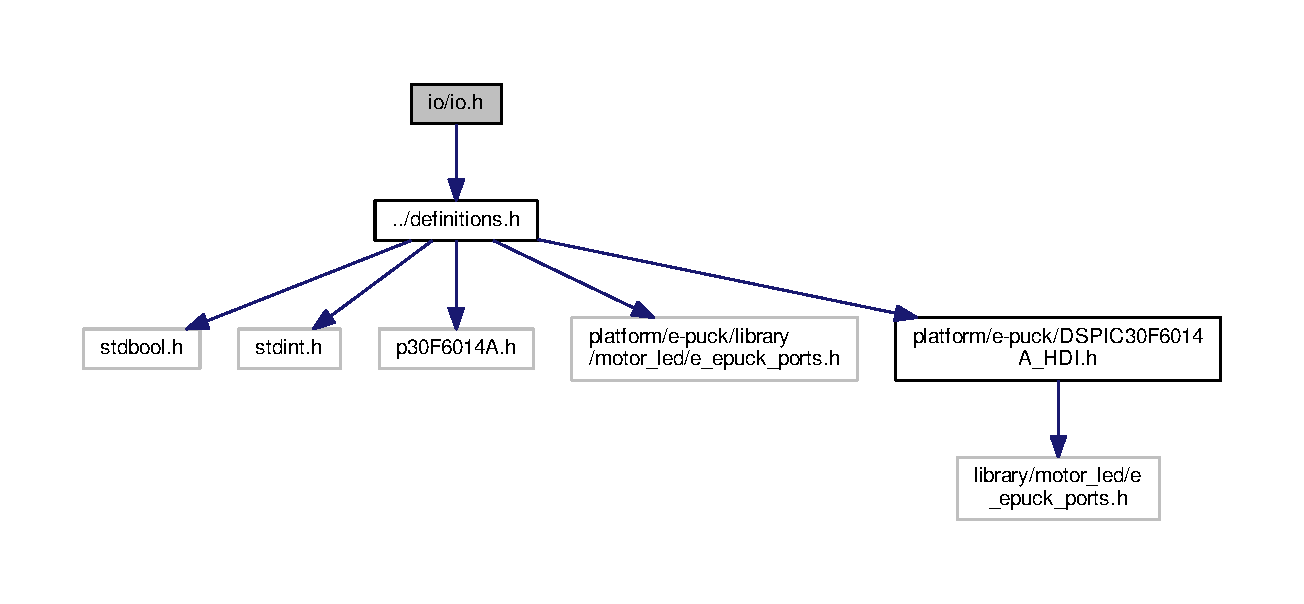
\includegraphics[width=350pt]{d8/da5/io_8h__incl}
\end{center}
\end{figure}
This graph shows which files directly or indirectly include this file\+:\nopagebreak
\begin{figure}[H]
\begin{center}
\leavevmode
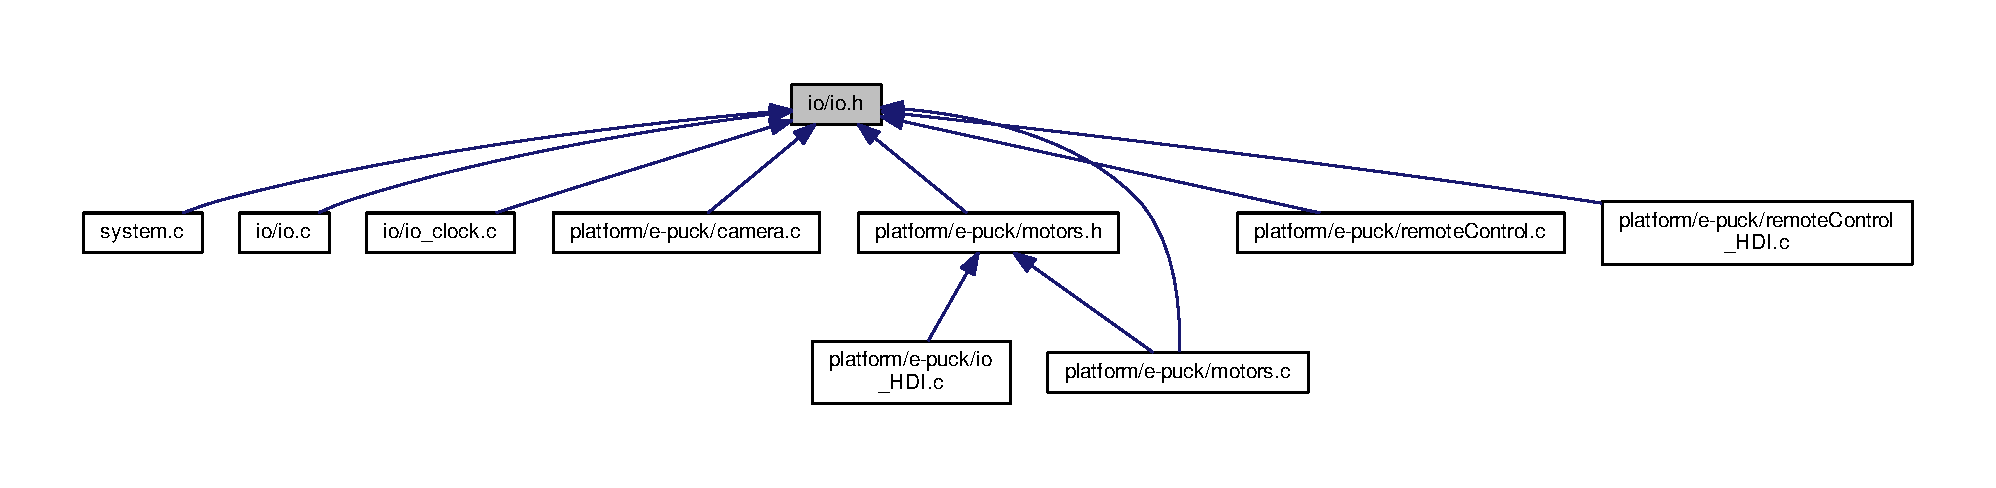
\includegraphics[width=350pt]{da/de4/io_8h__dep__incl}
\end{center}
\end{figure}
\subsection*{Functions}
\begin{DoxyCompactItemize}
\item 
void \hyperlink{io_8h_ad1719208a5855f34e056a8114de973f9}{Sys\+\_\+\+Init\+\_\+\+I\+O\+Management} (void)
\item 
void \hyperlink{io_8h_a6ca66df90d159586d58a19e01f3a7025}{Sys\+\_\+\+Start\+\_\+\+I\+O\+Management} (void)
\item 
void \hyperlink{io_8h_a14d9a8f941c03184049f3bf18d35fb47}{Sys\+\_\+\+Stop\+\_\+\+I\+O\+Management} (void)
\item 
void \hyperlink{io_8h_a3aa1e95e0e5be1866738b77f5b504652}{Sys\+\_\+\+Stop\+\_\+\+I\+O\+Timer} (void)
\item 
void \hyperlink{io_8h_a15a4d1cf4ffaac43d2c1ae131652b869}{Sys\+\_\+\+Continue\+\_\+\+I\+O\+Timer} (void)
\item 
void \hyperlink{io_8h_a022c90f875bdb0b3cf2c85ab7872f531}{Sys\+\_\+\+Reset\+\_\+\+I\+O\+Timer} (void)
\item 
void \hyperlink{io_8h_a21ac049cc8b67f8851decbbd0edf9dd6}{Sys\+\_\+\+Disable\+\_\+\+I\+O\+Timer\+Interrupt} (void)
\item 
void \hyperlink{io_8h_aefef1e8eb442327a4b4c7bc89d6d13ce}{Sys\+\_\+\+Enable\+\_\+\+I\+O\+Timer\+Interrupt} (void)
\item 
void \hyperlink{io_8h_ac23e12fcd2478b2d820aa55dcd9460ee}{Sys\+\_\+\+Force\+\_\+\+I\+O\+Timer\+Interrupt} (void)
\item 
bool \hyperlink{io_8h_a915425274eaebb4ed39d8622b90993b7}{Sys\+\_\+\+Register\+\_\+\+I\+O\+Handler} (\hyperlink{definitions_8h_aed53e618f2025481fbe48a5098f70079}{p\+Function} func)
\item 
void \hyperlink{io_8h_a1b695aa5cbdf06b543b10b9661722d36}{Sys\+\_\+\+Unregister\+\_\+\+I\+O\+Handler} (\hyperlink{definitions_8h_aed53e618f2025481fbe48a5098f70079}{p\+Function} func)
\end{DoxyCompactItemize}


\subsection{Detailed Description}
This file includes the I\+O timer to start and stop the timer. This timer executes I\+O functions periodically. 

\begin{DoxyAuthor}{Author}
Stefan M. Trenkwalder \href{mailto:s.trenkwalder@openswarm.org}{\tt s.\+trenkwalder@openswarm.\+org} 
\end{DoxyAuthor}
\begin{DoxyVersion}{Version}
1.\+0
\end{DoxyVersion}
\begin{DoxyDate}{Date}
28 July 2015
\end{DoxyDate}
\begin{DoxyCopyright}{Copyright}
adapted Free\+B\+S\+D License (see \href{http://openswarm.org/license}{\tt http\+://openswarm.\+org/license}) 
\end{DoxyCopyright}


\subsection{Function Documentation}
\hypertarget{io_8h_a15a4d1cf4ffaac43d2c1ae131652b869}{}\index{io.\+h@{io.\+h}!Sys\+\_\+\+Continue\+\_\+\+I\+O\+Timer@{Sys\+\_\+\+Continue\+\_\+\+I\+O\+Timer}}
\index{Sys\+\_\+\+Continue\+\_\+\+I\+O\+Timer@{Sys\+\_\+\+Continue\+\_\+\+I\+O\+Timer}!io.\+h@{io.\+h}}
\subsubsection[{Sys\+\_\+\+Continue\+\_\+\+I\+O\+Timer}]{\setlength{\rightskip}{0pt plus 5cm}void Sys\+\_\+\+Continue\+\_\+\+I\+O\+Timer (
\begin{DoxyParamCaption}
\item[{void}]{}
\end{DoxyParamCaption}
)\hspace{0.3cm}{\ttfamily [inline]}}\label{io_8h_a15a4d1cf4ffaac43d2c1ae131652b869}
Continues the I/\+O Timer

This function continues the I/\+O Timer. Note that the timer continues to count where it stops. 

Definition at line 71 of file io.\+c.

\hypertarget{io_8h_a21ac049cc8b67f8851decbbd0edf9dd6}{}\index{io.\+h@{io.\+h}!Sys\+\_\+\+Disable\+\_\+\+I\+O\+Timer\+Interrupt@{Sys\+\_\+\+Disable\+\_\+\+I\+O\+Timer\+Interrupt}}
\index{Sys\+\_\+\+Disable\+\_\+\+I\+O\+Timer\+Interrupt@{Sys\+\_\+\+Disable\+\_\+\+I\+O\+Timer\+Interrupt}!io.\+h@{io.\+h}}
\subsubsection[{Sys\+\_\+\+Disable\+\_\+\+I\+O\+Timer\+Interrupt}]{\setlength{\rightskip}{0pt plus 5cm}void Sys\+\_\+\+Disable\+\_\+\+I\+O\+Timer\+Interrupt (
\begin{DoxyParamCaption}
\item[{void}]{}
\end{DoxyParamCaption}
)\hspace{0.3cm}{\ttfamily [inline]}}\label{io_8h_a21ac049cc8b67f8851decbbd0edf9dd6}
Disables the I/\+O Timer

This function disables the I/\+O Timer interrupt. Note that the timer still continues to count. 

Definition at line 91 of file io.\+c.

\hypertarget{io_8h_aefef1e8eb442327a4b4c7bc89d6d13ce}{}\index{io.\+h@{io.\+h}!Sys\+\_\+\+Enable\+\_\+\+I\+O\+Timer\+Interrupt@{Sys\+\_\+\+Enable\+\_\+\+I\+O\+Timer\+Interrupt}}
\index{Sys\+\_\+\+Enable\+\_\+\+I\+O\+Timer\+Interrupt@{Sys\+\_\+\+Enable\+\_\+\+I\+O\+Timer\+Interrupt}!io.\+h@{io.\+h}}
\subsubsection[{Sys\+\_\+\+Enable\+\_\+\+I\+O\+Timer\+Interrupt}]{\setlength{\rightskip}{0pt plus 5cm}void Sys\+\_\+\+Enable\+\_\+\+I\+O\+Timer\+Interrupt (
\begin{DoxyParamCaption}
\item[{void}]{}
\end{DoxyParamCaption}
)\hspace{0.3cm}{\ttfamily [inline]}}\label{io_8h_aefef1e8eb442327a4b4c7bc89d6d13ce}
Enables the I/\+O Timer

This function enables the I/\+O Timer interrupt. 

Definition at line 101 of file io.\+c.

\hypertarget{io_8h_ac23e12fcd2478b2d820aa55dcd9460ee}{}\index{io.\+h@{io.\+h}!Sys\+\_\+\+Force\+\_\+\+I\+O\+Timer\+Interrupt@{Sys\+\_\+\+Force\+\_\+\+I\+O\+Timer\+Interrupt}}
\index{Sys\+\_\+\+Force\+\_\+\+I\+O\+Timer\+Interrupt@{Sys\+\_\+\+Force\+\_\+\+I\+O\+Timer\+Interrupt}!io.\+h@{io.\+h}}
\subsubsection[{Sys\+\_\+\+Force\+\_\+\+I\+O\+Timer\+Interrupt}]{\setlength{\rightskip}{0pt plus 5cm}void Sys\+\_\+\+Force\+\_\+\+I\+O\+Timer\+Interrupt (
\begin{DoxyParamCaption}
\item[{void}]{}
\end{DoxyParamCaption}
)\hspace{0.3cm}{\ttfamily [inline]}}\label{io_8h_ac23e12fcd2478b2d820aa55dcd9460ee}
Force the I/\+O Timer interrupt.

This function forces a new I/\+O Timer interrupt even if the timer hasn\textquotesingle{}t reached its threshold. 

Definition at line 111 of file io.\+c.

\hypertarget{io_8h_ad1719208a5855f34e056a8114de973f9}{}\index{io.\+h@{io.\+h}!Sys\+\_\+\+Init\+\_\+\+I\+O\+Management@{Sys\+\_\+\+Init\+\_\+\+I\+O\+Management}}
\index{Sys\+\_\+\+Init\+\_\+\+I\+O\+Management@{Sys\+\_\+\+Init\+\_\+\+I\+O\+Management}!io.\+h@{io.\+h}}
\subsubsection[{Sys\+\_\+\+Init\+\_\+\+I\+O\+Management}]{\setlength{\rightskip}{0pt plus 5cm}void Sys\+\_\+\+Init\+\_\+\+I\+O\+Management (
\begin{DoxyParamCaption}
\item[{void}]{}
\end{DoxyParamCaption}
)\hspace{0.3cm}{\ttfamily [inline]}}\label{io_8h_ad1719208a5855f34e056a8114de973f9}
Initialises the I/\+O Management

This function initialises the I/\+O Timer and therefore the I/\+O Management. 

Definition at line 31 of file io.\+c.

\hypertarget{io_8h_a915425274eaebb4ed39d8622b90993b7}{}\index{io.\+h@{io.\+h}!Sys\+\_\+\+Register\+\_\+\+I\+O\+Handler@{Sys\+\_\+\+Register\+\_\+\+I\+O\+Handler}}
\index{Sys\+\_\+\+Register\+\_\+\+I\+O\+Handler@{Sys\+\_\+\+Register\+\_\+\+I\+O\+Handler}!io.\+h@{io.\+h}}
\subsubsection[{Sys\+\_\+\+Register\+\_\+\+I\+O\+Handler}]{\setlength{\rightskip}{0pt plus 5cm}bool Sys\+\_\+\+Register\+\_\+\+I\+O\+Handler (
\begin{DoxyParamCaption}
\item[{{\bf p\+Function}}]{func}
\end{DoxyParamCaption}
)}\label{io_8h_a915425274eaebb4ed39d8622b90993b7}
registers new I/\+O handler.

This function registers a new I/\+O handler which is executed every time the I/\+O timer interrupt occurs.


\begin{DoxyParams}{Parameters}
{\em func} & pointer to the function that should be executed by the I/\+O timer periodically \\
\hline
\end{DoxyParams}
\begin{DoxyReturn}{Returns}
bool was it successful? 
\end{DoxyReturn}


Definition at line 123 of file io.\+c.

\hypertarget{io_8h_a022c90f875bdb0b3cf2c85ab7872f531}{}\index{io.\+h@{io.\+h}!Sys\+\_\+\+Reset\+\_\+\+I\+O\+Timer@{Sys\+\_\+\+Reset\+\_\+\+I\+O\+Timer}}
\index{Sys\+\_\+\+Reset\+\_\+\+I\+O\+Timer@{Sys\+\_\+\+Reset\+\_\+\+I\+O\+Timer}!io.\+h@{io.\+h}}
\subsubsection[{Sys\+\_\+\+Reset\+\_\+\+I\+O\+Timer}]{\setlength{\rightskip}{0pt plus 5cm}void Sys\+\_\+\+Reset\+\_\+\+I\+O\+Timer (
\begin{DoxyParamCaption}
\item[{void}]{}
\end{DoxyParamCaption}
)\hspace{0.3cm}{\ttfamily [inline]}}\label{io_8h_a022c90f875bdb0b3cf2c85ab7872f531}
resets the I/\+O Timer

This function sets the I/\+O Timer counter to 0 and the I/\+O timer needs the full time duration to throw the interrupt. 

Definition at line 81 of file io.\+c.

\hypertarget{io_8h_a6ca66df90d159586d58a19e01f3a7025}{}\index{io.\+h@{io.\+h}!Sys\+\_\+\+Start\+\_\+\+I\+O\+Management@{Sys\+\_\+\+Start\+\_\+\+I\+O\+Management}}
\index{Sys\+\_\+\+Start\+\_\+\+I\+O\+Management@{Sys\+\_\+\+Start\+\_\+\+I\+O\+Management}!io.\+h@{io.\+h}}
\subsubsection[{Sys\+\_\+\+Start\+\_\+\+I\+O\+Management}]{\setlength{\rightskip}{0pt plus 5cm}void Sys\+\_\+\+Start\+\_\+\+I\+O\+Management (
\begin{DoxyParamCaption}
\item[{void}]{}
\end{DoxyParamCaption}
)\hspace{0.3cm}{\ttfamily [inline]}}\label{io_8h_a6ca66df90d159586d58a19e01f3a7025}
Starts the I/\+O Management

This function starts the I/\+O Timer and therefore the I/\+O Management. 

Definition at line 41 of file io.\+c.

\hypertarget{io_8h_a14d9a8f941c03184049f3bf18d35fb47}{}\index{io.\+h@{io.\+h}!Sys\+\_\+\+Stop\+\_\+\+I\+O\+Management@{Sys\+\_\+\+Stop\+\_\+\+I\+O\+Management}}
\index{Sys\+\_\+\+Stop\+\_\+\+I\+O\+Management@{Sys\+\_\+\+Stop\+\_\+\+I\+O\+Management}!io.\+h@{io.\+h}}
\subsubsection[{Sys\+\_\+\+Stop\+\_\+\+I\+O\+Management}]{\setlength{\rightskip}{0pt plus 5cm}void Sys\+\_\+\+Stop\+\_\+\+I\+O\+Management (
\begin{DoxyParamCaption}
\item[{void}]{}
\end{DoxyParamCaption}
)\hspace{0.3cm}{\ttfamily [inline]}}\label{io_8h_a14d9a8f941c03184049f3bf18d35fb47}
Stops the I/\+O Management

This function stops the I/\+O Timer and therefore the I/\+O Management. 

Definition at line 51 of file io.\+c.

\hypertarget{io_8h_a3aa1e95e0e5be1866738b77f5b504652}{}\index{io.\+h@{io.\+h}!Sys\+\_\+\+Stop\+\_\+\+I\+O\+Timer@{Sys\+\_\+\+Stop\+\_\+\+I\+O\+Timer}}
\index{Sys\+\_\+\+Stop\+\_\+\+I\+O\+Timer@{Sys\+\_\+\+Stop\+\_\+\+I\+O\+Timer}!io.\+h@{io.\+h}}
\subsubsection[{Sys\+\_\+\+Stop\+\_\+\+I\+O\+Timer}]{\setlength{\rightskip}{0pt plus 5cm}void Sys\+\_\+\+Stop\+\_\+\+I\+O\+Timer (
\begin{DoxyParamCaption}
\item[{void}]{}
\end{DoxyParamCaption}
)\hspace{0.3cm}{\ttfamily [inline]}}\label{io_8h_a3aa1e95e0e5be1866738b77f5b504652}
Stops the I/\+O Timer

This function stops the I/\+O Timer. 

Definition at line 61 of file io.\+c.

\hypertarget{io_8h_a1b695aa5cbdf06b543b10b9661722d36}{}\index{io.\+h@{io.\+h}!Sys\+\_\+\+Unregister\+\_\+\+I\+O\+Handler@{Sys\+\_\+\+Unregister\+\_\+\+I\+O\+Handler}}
\index{Sys\+\_\+\+Unregister\+\_\+\+I\+O\+Handler@{Sys\+\_\+\+Unregister\+\_\+\+I\+O\+Handler}!io.\+h@{io.\+h}}
\subsubsection[{Sys\+\_\+\+Unregister\+\_\+\+I\+O\+Handler}]{\setlength{\rightskip}{0pt plus 5cm}void Sys\+\_\+\+Unregister\+\_\+\+I\+O\+Handler (
\begin{DoxyParamCaption}
\item[{{\bf p\+Function}}]{func}
\end{DoxyParamCaption}
)}\label{io_8h_a1b695aa5cbdf06b543b10b9661722d36}
unregisters new I/\+O handler.

This function unregisters a I/\+O handler identified by its function address.


\begin{DoxyParams}{Parameters}
{\em func} & pointer to the function that should be executed by the I/\+O timer periodically \\
\hline
\end{DoxyParams}


Definition at line 158 of file io.\+c.


\hypertarget{io__clock_8c}{}\subsection{io/io\+\_\+clock.c File Reference}
\label{io__clock_8c}\index{io/io\+\_\+clock.\+c@{io/io\+\_\+clock.\+c}}


It defines the system clock that provides a continuous time value (granulation of 1 ms).  


{\ttfamily \#include \char`\"{}io.\+h\char`\"{}}\\*
{\ttfamily \#include \char`\"{}io\+\_\+clock.\+h\char`\"{}}\\*
{\ttfamily \#include \char`\"{}e-\/puck/io\+\_\+\+H\+D\+I.\+h\char`\"{}}\\*
{\ttfamily \#include \char`\"{}../events/events.\+h\char`\"{}}\\*
Include dependency graph for io\+\_\+clock.\+c\+:\nopagebreak
\begin{figure}[H]
\begin{center}
\leavevmode
\includegraphics[width=350pt]{d1/d5c/io__clock_8c__incl}
\end{center}
\end{figure}
\subsubsection*{Functions}
\begin{DoxyCompactItemize}
\item 
void \hyperlink{io__clock_8c_a6664a6f3068df96c1b85eaa4f0d5fd6a}{Sys\+\_\+\+System\+Clock\+\_\+\+Counter} (void)
\item 
void \hyperlink{io__clock_8c_a63a0287d2d658db8dd16e048030213a5}{Sys\+\_\+\+Init\+\_\+\+Clock} ()
\item 
void \hyperlink{io__clock_8c_a17ff576103f640d63707b2dbf13b28c7}{Sys\+\_\+\+Init\+\_\+\+System\+Time} ()
\item 
\hyperlink{definitions_8h_a1134b580f8da4de94ca6b1de4d37975e}{uint32} \hyperlink{io__clock_8c_a3df05c406decdffd415aeb1dd8347933}{Sys\+\_\+\+Get\+\_\+\+System\+Time} ()
\item 
\hyperlink{definitions_8h_a1134b580f8da4de94ca6b1de4d37975e}{uint32} \hyperlink{io__clock_8c_afb5189028721e3deac5a210b4da93b3a}{Sys\+\_\+\+Get\+\_\+\+System\+Clock} ()
\end{DoxyCompactItemize}


\subsubsection{Detailed Description}
It defines the system clock that provides a continuous time value (granulation of 1 ms). 

\begin{DoxyAuthor}{Author}
Stefan M. Trenkwalder \href{mailto:s.trenkwalder@openswarm.org}{\tt s.\+trenkwalder@openswarm.\+org} 
\end{DoxyAuthor}
\begin{DoxyVersion}{Version}
1.\+0
\end{DoxyVersion}
\begin{DoxyDate}{Date}
28 July 2015
\end{DoxyDate}
\begin{DoxyCopyright}{Copyright}
adapted Free\+B\+S\+D License (see \href{http://openswarm.org/license}{\tt http\+://openswarm.\+org/license}) 
\end{DoxyCopyright}


\subsubsection{Function Documentation}
\hypertarget{io__clock_8c_afb5189028721e3deac5a210b4da93b3a}{}\index{io\+\_\+clock.\+c@{io\+\_\+clock.\+c}!Sys\+\_\+\+Get\+\_\+\+System\+Clock@{Sys\+\_\+\+Get\+\_\+\+System\+Clock}}
\index{Sys\+\_\+\+Get\+\_\+\+System\+Clock@{Sys\+\_\+\+Get\+\_\+\+System\+Clock}!io\+\_\+clock.\+c@{io\+\_\+clock.\+c}}
\paragraph[{Sys\+\_\+\+Get\+\_\+\+System\+Clock}]{\setlength{\rightskip}{0pt plus 5cm}{\bf uint32} Sys\+\_\+\+Get\+\_\+\+System\+Clock (
\begin{DoxyParamCaption}
\item[{void}]{}
\end{DoxyParamCaption}
)\hspace{0.3cm}{\ttfamily [inline]}}\label{io__clock_8c_afb5189028721e3deac5a210b4da93b3a}
returns the system clock/time in milliseconds

\begin{DoxyReturn}{Returns}
uint32 time that has passed since Open\+Swarm was started 
\end{DoxyReturn}


Definition at line 77 of file io\+\_\+clock.\+c.

\hypertarget{io__clock_8c_a3df05c406decdffd415aeb1dd8347933}{}\index{io\+\_\+clock.\+c@{io\+\_\+clock.\+c}!Sys\+\_\+\+Get\+\_\+\+System\+Time@{Sys\+\_\+\+Get\+\_\+\+System\+Time}}
\index{Sys\+\_\+\+Get\+\_\+\+System\+Time@{Sys\+\_\+\+Get\+\_\+\+System\+Time}!io\+\_\+clock.\+c@{io\+\_\+clock.\+c}}
\paragraph[{Sys\+\_\+\+Get\+\_\+\+System\+Time}]{\setlength{\rightskip}{0pt plus 5cm}{\bf uint32} Sys\+\_\+\+Get\+\_\+\+System\+Time (
\begin{DoxyParamCaption}
\item[{void}]{}
\end{DoxyParamCaption}
)\hspace{0.3cm}{\ttfamily [inline]}}\label{io__clock_8c_a3df05c406decdffd415aeb1dd8347933}
Renaming of the function \hyperlink{io__clock_8c_afb5189028721e3deac5a210b4da93b3a}{Sys\+\_\+\+Get\+\_\+\+System\+Clock()}.

\begin{DoxyReturn}{Returns}
time that has passed since Open\+Swarm was started (uint32) 
\end{DoxyReturn}


Definition at line 67 of file io\+\_\+clock.\+c.

\hypertarget{io__clock_8c_a63a0287d2d658db8dd16e048030213a5}{}\index{io\+\_\+clock.\+c@{io\+\_\+clock.\+c}!Sys\+\_\+\+Init\+\_\+\+Clock@{Sys\+\_\+\+Init\+\_\+\+Clock}}
\index{Sys\+\_\+\+Init\+\_\+\+Clock@{Sys\+\_\+\+Init\+\_\+\+Clock}!io\+\_\+clock.\+c@{io\+\_\+clock.\+c}}
\paragraph[{Sys\+\_\+\+Init\+\_\+\+Clock}]{\setlength{\rightskip}{0pt plus 5cm}void Sys\+\_\+\+Init\+\_\+\+Clock (
\begin{DoxyParamCaption}
\item[{void}]{}
\end{DoxyParamCaption}
)\hspace{0.3cm}{\ttfamily [inline]}}\label{io__clock_8c_a63a0287d2d658db8dd16e048030213a5}
This function initialises the system clock which is in principle a counter that inicates passed milli seconds. $<$ I\+D of the event that signals 1ms timer ticks 

Definition at line 29 of file io\+\_\+clock.\+c.

\hypertarget{io__clock_8c_a17ff576103f640d63707b2dbf13b28c7}{}\index{io\+\_\+clock.\+c@{io\+\_\+clock.\+c}!Sys\+\_\+\+Init\+\_\+\+System\+Time@{Sys\+\_\+\+Init\+\_\+\+System\+Time}}
\index{Sys\+\_\+\+Init\+\_\+\+System\+Time@{Sys\+\_\+\+Init\+\_\+\+System\+Time}!io\+\_\+clock.\+c@{io\+\_\+clock.\+c}}
\paragraph[{Sys\+\_\+\+Init\+\_\+\+System\+Time}]{\setlength{\rightskip}{0pt plus 5cm}void Sys\+\_\+\+Init\+\_\+\+System\+Time (
\begin{DoxyParamCaption}
\item[{void}]{}
\end{DoxyParamCaption}
)\hspace{0.3cm}{\ttfamily [inline]}}\label{io__clock_8c_a17ff576103f640d63707b2dbf13b28c7}
Renaming of the function \hyperlink{io__clock_8c_a63a0287d2d658db8dd16e048030213a5}{Sys\+\_\+\+Init\+\_\+\+Clock()}. 

Definition at line 39 of file io\+\_\+clock.\+c.

\hypertarget{io__clock_8c_a6664a6f3068df96c1b85eaa4f0d5fd6a}{}\index{io\+\_\+clock.\+c@{io\+\_\+clock.\+c}!Sys\+\_\+\+System\+Clock\+\_\+\+Counter@{Sys\+\_\+\+System\+Clock\+\_\+\+Counter}}
\index{Sys\+\_\+\+System\+Clock\+\_\+\+Counter@{Sys\+\_\+\+System\+Clock\+\_\+\+Counter}!io\+\_\+clock.\+c@{io\+\_\+clock.\+c}}
\paragraph[{Sys\+\_\+\+System\+Clock\+\_\+\+Counter}]{\setlength{\rightskip}{0pt plus 5cm}void Sys\+\_\+\+System\+Clock\+\_\+\+Counter (
\begin{DoxyParamCaption}
{}
\end{DoxyParamCaption}
)}\label{io__clock_8c_a6664a6f3068df96c1b85eaa4f0d5fd6a}
This function calculates the system clock tick and increases the counter if a millisecond passed. $<$ I\+D of the event that signals 1ms timer ticks 

Definition at line 48 of file io\+\_\+clock.\+c.


\hypertarget{io__clock_8h}{}\section{io/io\+\_\+clock.h File Reference}
\label{io__clock_8h}\index{io/io\+\_\+clock.\+h@{io/io\+\_\+clock.\+h}}


declares the system clock that provides a continuous time value (granulation of 1 ms).  


{\ttfamily \#include \char`\"{}../definitions.\+h\char`\"{}}\\*
Include dependency graph for io\+\_\+clock.\+h\+:
\nopagebreak
\begin{figure}[H]
\begin{center}
\leavevmode
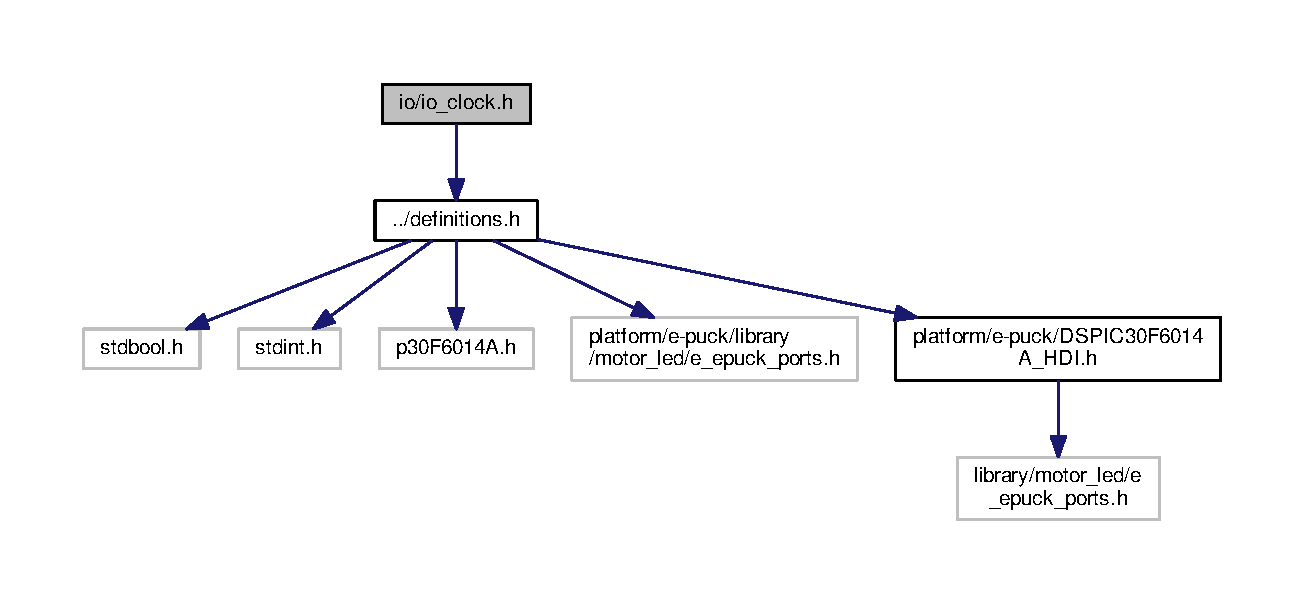
\includegraphics[width=350pt]{d5/de6/io__clock_8h__incl}
\end{center}
\end{figure}
This graph shows which files directly or indirectly include this file\+:
\nopagebreak
\begin{figure}[H]
\begin{center}
\leavevmode
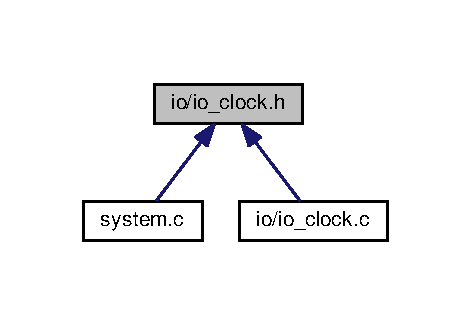
\includegraphics[width=226pt]{d6/d4c/io__clock_8h__dep__incl}
\end{center}
\end{figure}
\subsection*{Functions}
\begin{DoxyCompactItemize}
\item 
void \hyperlink{io__clock_8h_a236ed02217a4cf5eaa9a0fd340debbd6}{Sys\+\_\+\+Init\+\_\+\+Clock} (void)
\item 
void \hyperlink{io__clock_8h_a999ca0e97c3879e10c59f10d29b7e674}{Sys\+\_\+\+Init\+\_\+\+System\+Time} (void)
\item 
\hyperlink{definitions_8h_a1134b580f8da4de94ca6b1de4d37975e}{uint32} \hyperlink{io__clock_8h_aa6787b3374d37d49863aaec1317e363a}{Sys\+\_\+\+Get\+\_\+\+System\+Time} (void)
\item 
\hyperlink{definitions_8h_a1134b580f8da4de94ca6b1de4d37975e}{uint32} \hyperlink{io__clock_8h_a60f9d3d6edf35a4bbda01d2c1b9d3f96}{Sys\+\_\+\+Get\+\_\+\+System\+Clock} (void)
\end{DoxyCompactItemize}


\subsection{Detailed Description}
declares the system clock that provides a continuous time value (granulation of 1 ms). 

\begin{DoxyAuthor}{Author}
Stefan M. Trenkwalder \href{mailto:s.trenkwalder@openswarm.org}{\tt s.\+trenkwalder@openswarm.\+org} 
\end{DoxyAuthor}
\begin{DoxyVersion}{Version}
1.\+0
\end{DoxyVersion}
\begin{DoxyDate}{Date}
28 July 2015
\end{DoxyDate}
\begin{DoxyCopyright}{Copyright}
adapted Free\+B\+S\+D License (see \href{http://openswarm.org/license}{\tt http\+://openswarm.\+org/license}) 
\end{DoxyCopyright}


\subsection{Function Documentation}
\hypertarget{io__clock_8h_a60f9d3d6edf35a4bbda01d2c1b9d3f96}{}\index{io\+\_\+clock.\+h@{io\+\_\+clock.\+h}!Sys\+\_\+\+Get\+\_\+\+System\+Clock@{Sys\+\_\+\+Get\+\_\+\+System\+Clock}}
\index{Sys\+\_\+\+Get\+\_\+\+System\+Clock@{Sys\+\_\+\+Get\+\_\+\+System\+Clock}!io\+\_\+clock.\+h@{io\+\_\+clock.\+h}}
\subsubsection[{Sys\+\_\+\+Get\+\_\+\+System\+Clock}]{\setlength{\rightskip}{0pt plus 5cm}{\bf uint32} Sys\+\_\+\+Get\+\_\+\+System\+Clock (
\begin{DoxyParamCaption}
\item[{void}]{}
\end{DoxyParamCaption}
)\hspace{0.3cm}{\ttfamily [inline]}}\label{io__clock_8h_a60f9d3d6edf35a4bbda01d2c1b9d3f96}
returns the system clock/time in milliseconds

returns the system clock/time in milliseconds

\begin{DoxyReturn}{Returns}
uint32 time that has passed since Open\+Swarm was started 
\end{DoxyReturn}


Definition at line 82 of file io\+\_\+clock.\+c.

\hypertarget{io__clock_8h_aa6787b3374d37d49863aaec1317e363a}{}\index{io\+\_\+clock.\+h@{io\+\_\+clock.\+h}!Sys\+\_\+\+Get\+\_\+\+System\+Time@{Sys\+\_\+\+Get\+\_\+\+System\+Time}}
\index{Sys\+\_\+\+Get\+\_\+\+System\+Time@{Sys\+\_\+\+Get\+\_\+\+System\+Time}!io\+\_\+clock.\+h@{io\+\_\+clock.\+h}}
\subsubsection[{Sys\+\_\+\+Get\+\_\+\+System\+Time}]{\setlength{\rightskip}{0pt plus 5cm}{\bf uint32} Sys\+\_\+\+Get\+\_\+\+System\+Time (
\begin{DoxyParamCaption}
\item[{void}]{}
\end{DoxyParamCaption}
)\hspace{0.3cm}{\ttfamily [inline]}}\label{io__clock_8h_aa6787b3374d37d49863aaec1317e363a}
Renaming of the function \hyperlink{io__clock_8c_afb5189028721e3deac5a210b4da93b3a}{Sys\+\_\+\+Get\+\_\+\+System\+Clock()}.

Renaming of the function \hyperlink{io__clock_8c_afb5189028721e3deac5a210b4da93b3a}{Sys\+\_\+\+Get\+\_\+\+System\+Clock()}.

\begin{DoxyReturn}{Returns}
uint32 time that has passed since Open\+Swarm was started 
\end{DoxyReturn}


Definition at line 71 of file io\+\_\+clock.\+c.

\hypertarget{io__clock_8h_a236ed02217a4cf5eaa9a0fd340debbd6}{}\index{io\+\_\+clock.\+h@{io\+\_\+clock.\+h}!Sys\+\_\+\+Init\+\_\+\+Clock@{Sys\+\_\+\+Init\+\_\+\+Clock}}
\index{Sys\+\_\+\+Init\+\_\+\+Clock@{Sys\+\_\+\+Init\+\_\+\+Clock}!io\+\_\+clock.\+h@{io\+\_\+clock.\+h}}
\subsubsection[{Sys\+\_\+\+Init\+\_\+\+Clock}]{\setlength{\rightskip}{0pt plus 5cm}void Sys\+\_\+\+Init\+\_\+\+Clock (
\begin{DoxyParamCaption}
\item[{void}]{}
\end{DoxyParamCaption}
)\hspace{0.3cm}{\ttfamily [inline]}}\label{io__clock_8h_a236ed02217a4cf5eaa9a0fd340debbd6}
This function initialises the system clock

This function initialises the system clock which is in principle a counter that inicates passed milli seconds. 

Definition at line 30 of file io\+\_\+clock.\+c.

\hypertarget{io__clock_8h_a999ca0e97c3879e10c59f10d29b7e674}{}\index{io\+\_\+clock.\+h@{io\+\_\+clock.\+h}!Sys\+\_\+\+Init\+\_\+\+System\+Time@{Sys\+\_\+\+Init\+\_\+\+System\+Time}}
\index{Sys\+\_\+\+Init\+\_\+\+System\+Time@{Sys\+\_\+\+Init\+\_\+\+System\+Time}!io\+\_\+clock.\+h@{io\+\_\+clock.\+h}}
\subsubsection[{Sys\+\_\+\+Init\+\_\+\+System\+Time}]{\setlength{\rightskip}{0pt plus 5cm}void Sys\+\_\+\+Init\+\_\+\+System\+Time (
\begin{DoxyParamCaption}
\item[{void}]{}
\end{DoxyParamCaption}
)\hspace{0.3cm}{\ttfamily [inline]}}\label{io__clock_8h_a999ca0e97c3879e10c59f10d29b7e674}
Renaming of the function \hyperlink{io__clock_8c_a63a0287d2d658db8dd16e048030213a5}{Sys\+\_\+\+Init\+\_\+\+Clock()}.

Renaming of the function \hyperlink{io__clock_8c_a63a0287d2d658db8dd16e048030213a5}{Sys\+\_\+\+Init\+\_\+\+Clock()}. 

Definition at line 41 of file io\+\_\+clock.\+c.


\hypertarget{memory_8c}{}\section{memory.\+c File Reference}
\label{memory_8c}\index{memory.\+c@{memory.\+c}}


includes functions to allocate, free, and copy memory  


{\ttfamily \#include \char`\"{}memory.\+h\char`\"{}}\\*
{\ttfamily \#include \char`\"{}interrupts.\+h\char`\"{}}\\*
{\ttfamily \#include $<$stdlib.\+h$>$}\\*
Include dependency graph for memory.\+c\+:\nopagebreak
\begin{figure}[H]
\begin{center}
\leavevmode
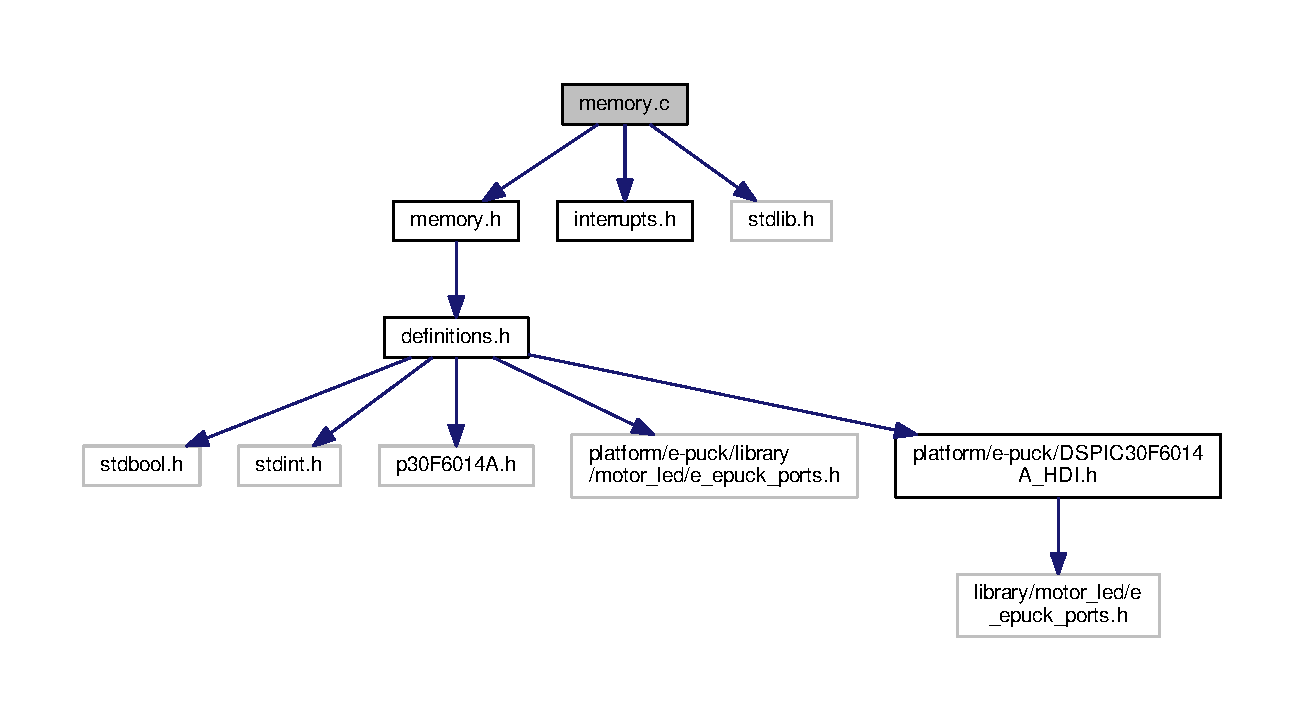
\includegraphics[width=350pt]{d1/dcd/memory_8c__incl}
\end{center}
\end{figure}
\subsection*{Functions}
\begin{DoxyCompactItemize}
\item 
void $\ast$ \hyperlink{memory_8c_aac1292ecd85eefecced84ec282250442}{Sys\+\_\+\+Malloc} (\hyperlink{definitions_8h_a05f6b0ae8f6a6e135b0e290c25fe0e4e}{uint16} length)
\item 
void \hyperlink{memory_8c_aab581d2999681f3bc60bcf46a59dfb35}{Sys\+\_\+\+Free} (void $\ast$data)
\item 
void \hyperlink{memory_8c_a0529ac1dbd051c6866093fc1493abf79}{Sys\+\_\+\+Memcpy} (void $\ast$source\+\_\+i, void $\ast$destination\+\_\+o, \hyperlink{definitions_8h_a05f6b0ae8f6a6e135b0e290c25fe0e4e}{uint16} length)
\end{DoxyCompactItemize}


\subsection{Detailed Description}
includes functions to allocate, free, and copy memory 

\begin{DoxyAuthor}{Author}
Stefan M. Trenkwalder \href{mailto:s.trenkwalder@openswarm.org}{\tt s.\+trenkwalder@openswarm.\+org} 
\end{DoxyAuthor}
\begin{DoxyVersion}{Version}
1.\+0
\end{DoxyVersion}
\begin{DoxyDate}{Date}
\{05 September 2015\}
\end{DoxyDate}
\begin{DoxyCopyright}{Copyright}
adapted Free\+B\+S\+D License (see \href{http://openswarm.org/license}{\tt http\+://openswarm.\+org/license}) 
\end{DoxyCopyright}


\subsection{Function Documentation}
\hypertarget{memory_8c_aab581d2999681f3bc60bcf46a59dfb35}{}\index{memory.\+c@{memory.\+c}!Sys\+\_\+\+Free@{Sys\+\_\+\+Free}}
\index{Sys\+\_\+\+Free@{Sys\+\_\+\+Free}!memory.\+c@{memory.\+c}}
\subsubsection[{Sys\+\_\+\+Free}]{\setlength{\rightskip}{0pt plus 5cm}void Sys\+\_\+\+Free (
\begin{DoxyParamCaption}
\item[{void $\ast$}]{data}
\end{DoxyParamCaption}
)}\label{memory_8c_aab581d2999681f3bc60bcf46a59dfb35}
Function to free memory

This Function frees dynamic allocated memory. This freeing is performed as atomic action.


\begin{DoxyParams}{Parameters}
{\em data} & pointer to memory that should be freed. \\
\hline
\end{DoxyParams}


Definition at line 45 of file memory.\+c.

\hypertarget{memory_8c_aac1292ecd85eefecced84ec282250442}{}\index{memory.\+c@{memory.\+c}!Sys\+\_\+\+Malloc@{Sys\+\_\+\+Malloc}}
\index{Sys\+\_\+\+Malloc@{Sys\+\_\+\+Malloc}!memory.\+c@{memory.\+c}}
\subsubsection[{Sys\+\_\+\+Malloc}]{\setlength{\rightskip}{0pt plus 5cm}void$\ast$ Sys\+\_\+\+Malloc (
\begin{DoxyParamCaption}
\item[{{\bf uint16}}]{length}
\end{DoxyParamCaption}
)}\label{memory_8c_aac1292ecd85eefecced84ec282250442}
Function to allocate {\bfseries length} bytes of memory

This Function allocates memory of the size {\bfseries length}. This allocation is performed as atomic action.


\begin{DoxyParams}{Parameters}
{\em length} & value how many bytes should be allocated \\
\hline
\end{DoxyParams}
\begin{DoxyReturn}{Returns}
pointer to the allocated memory 
\end{DoxyReturn}


Definition at line 26 of file memory.\+c.

\hypertarget{memory_8c_a0529ac1dbd051c6866093fc1493abf79}{}\index{memory.\+c@{memory.\+c}!Sys\+\_\+\+Memcpy@{Sys\+\_\+\+Memcpy}}
\index{Sys\+\_\+\+Memcpy@{Sys\+\_\+\+Memcpy}!memory.\+c@{memory.\+c}}
\subsubsection[{Sys\+\_\+\+Memcpy}]{\setlength{\rightskip}{0pt plus 5cm}void Sys\+\_\+\+Memcpy (
\begin{DoxyParamCaption}
\item[{void $\ast$}]{source\+\_\+i, }
\item[{void $\ast$}]{destination\+\_\+o, }
\item[{{\bf uint16}}]{length}
\end{DoxyParamCaption}
)}\label{memory_8c_a0529ac1dbd051c6866093fc1493abf79}
Function to copies memory of the size {\bfseries length} from {\bfseries source\+\_\+i} to {\bfseries destination\+\_\+o}.

Function to copies memory of the size {\bfseries length} from {\bfseries source\+\_\+i} to {\bfseries destination\+\_\+o}. This copying is performed as atomic action.


\begin{DoxyParams}{Parameters}
{\em source\+\_\+i} & pointer to the source \\
\hline
{\em destination\+\_\+o} & pointer to the destination \\
\hline
{\em length} & size of the memory that has to be copied \\
\hline
\end{DoxyParams}


Definition at line 64 of file memory.\+c.


\hypertarget{memory_8h}{}\section{memory.\+h File Reference}
\label{memory_8h}\index{memory.\+h@{memory.\+h}}


includes functions to allocate, free, and copy memory  


{\ttfamily \#include \char`\"{}definitions.\+h\char`\"{}}\\*
Include dependency graph for memory.\+h\+:\nopagebreak
\begin{figure}[H]
\begin{center}
\leavevmode
\includegraphics[width=350pt]{df/d9a/memory_8h__incl}
\end{center}
\end{figure}
This graph shows which files directly or indirectly include this file\+:\nopagebreak
\begin{figure}[H]
\begin{center}
\leavevmode
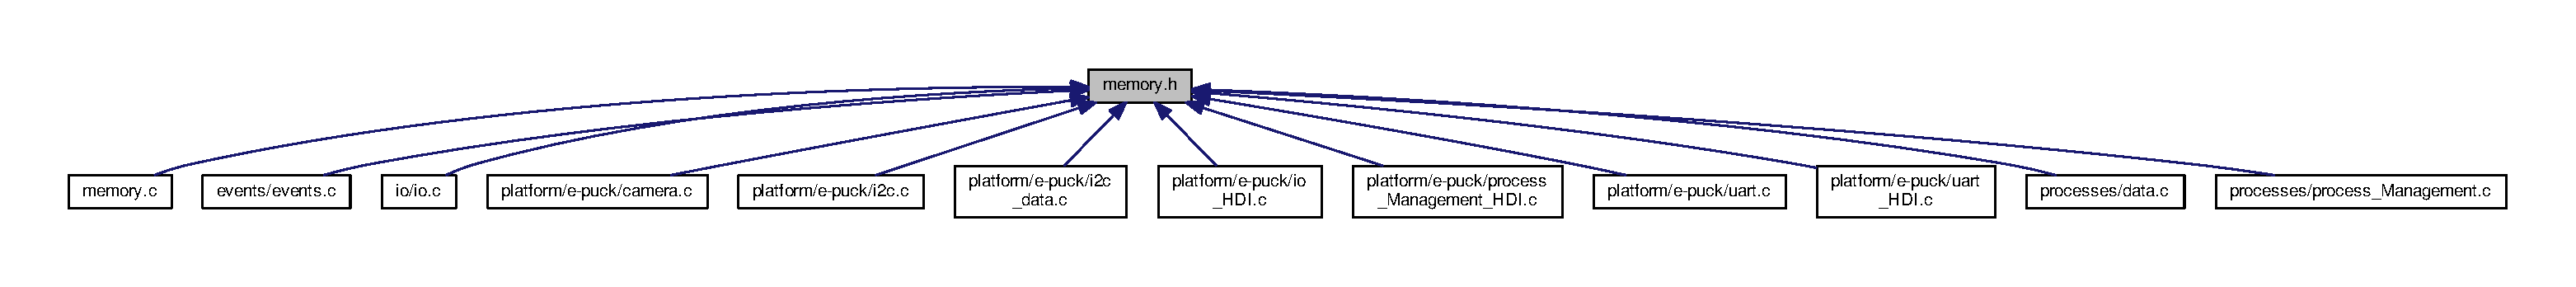
\includegraphics[width=350pt]{db/d57/memory_8h__dep__incl}
\end{center}
\end{figure}
\subsection*{Functions}
\begin{DoxyCompactItemize}
\item 
void $\ast$ \hyperlink{memory_8h_aac1292ecd85eefecced84ec282250442}{Sys\+\_\+\+Malloc} (\hyperlink{definitions_8h_a05f6b0ae8f6a6e135b0e290c25fe0e4e}{uint16} length)
\item 
void \hyperlink{memory_8h_a8f04ee5feb590ac9777b8c76c4d2cd70}{Sys\+\_\+\+Free} (void $\ast$)
\item 
void \hyperlink{memory_8h_ac496f9d5e3dc6b8644f137ad7d0e8bc4}{Sys\+\_\+\+Memcpy} (void $\ast$source, void $\ast$destination, \hyperlink{definitions_8h_a05f6b0ae8f6a6e135b0e290c25fe0e4e}{uint16} length)
\end{DoxyCompactItemize}


\subsection{Detailed Description}
includes functions to allocate, free, and copy memory 

\begin{DoxyAuthor}{Author}
Stefan M. Trenkwalder \href{mailto:s.trenkwalder@openswarm.org}{\tt s.\+trenkwalder@openswarm.\+org} 
\end{DoxyAuthor}
\begin{DoxyVersion}{Version}
1.\+0
\end{DoxyVersion}
\begin{DoxyDate}{Date}
\{05 September 2015\}
\end{DoxyDate}
\begin{DoxyCopyright}{Copyright}
adapted Free\+B\+S\+D License (see \href{http://openswarm.org/license}{\tt http\+://openswarm.\+org/license}) 
\end{DoxyCopyright}


\subsection{Function Documentation}
\hypertarget{memory_8h_a8f04ee5feb590ac9777b8c76c4d2cd70}{}\index{memory.\+h@{memory.\+h}!Sys\+\_\+\+Free@{Sys\+\_\+\+Free}}
\index{Sys\+\_\+\+Free@{Sys\+\_\+\+Free}!memory.\+h@{memory.\+h}}
\subsubsection[{Sys\+\_\+\+Free}]{\setlength{\rightskip}{0pt plus 5cm}void Sys\+\_\+\+Free (
\begin{DoxyParamCaption}
\item[{void $\ast$}]{data}
\end{DoxyParamCaption}
)}\label{memory_8h_a8f04ee5feb590ac9777b8c76c4d2cd70}
Function to free memory

This Function frees dynamic allocated memory. This freeing is performed as atomic action.


\begin{DoxyParams}{Parameters}
{\em data} & pointer to memory that should be freed. \\
\hline
\end{DoxyParams}


Definition at line 45 of file memory.\+c.

\hypertarget{memory_8h_aac1292ecd85eefecced84ec282250442}{}\index{memory.\+h@{memory.\+h}!Sys\+\_\+\+Malloc@{Sys\+\_\+\+Malloc}}
\index{Sys\+\_\+\+Malloc@{Sys\+\_\+\+Malloc}!memory.\+h@{memory.\+h}}
\subsubsection[{Sys\+\_\+\+Malloc}]{\setlength{\rightskip}{0pt plus 5cm}void$\ast$ Sys\+\_\+\+Malloc (
\begin{DoxyParamCaption}
\item[{{\bf uint16}}]{length}
\end{DoxyParamCaption}
)}\label{memory_8h_aac1292ecd85eefecced84ec282250442}
Function to allocate {\bfseries length} bytes of memory

This Function allocates memory of the size {\bfseries length}. This allocation is performed as atomic action.


\begin{DoxyParams}{Parameters}
{\em length} & value how many bytes should be allocated \\
\hline
\end{DoxyParams}
\begin{DoxyReturn}{Returns}
pointer to the allocated memory 
\end{DoxyReturn}


Definition at line 26 of file memory.\+c.

\hypertarget{memory_8h_ac496f9d5e3dc6b8644f137ad7d0e8bc4}{}\index{memory.\+h@{memory.\+h}!Sys\+\_\+\+Memcpy@{Sys\+\_\+\+Memcpy}}
\index{Sys\+\_\+\+Memcpy@{Sys\+\_\+\+Memcpy}!memory.\+h@{memory.\+h}}
\subsubsection[{Sys\+\_\+\+Memcpy}]{\setlength{\rightskip}{0pt plus 5cm}void Sys\+\_\+\+Memcpy (
\begin{DoxyParamCaption}
\item[{void $\ast$}]{source\+\_\+i, }
\item[{void $\ast$}]{destination\+\_\+o, }
\item[{{\bf uint16}}]{length}
\end{DoxyParamCaption}
)}\label{memory_8h_ac496f9d5e3dc6b8644f137ad7d0e8bc4}
Function to copies memory of the size {\bfseries length} from {\bfseries source\+\_\+i} to {\bfseries destination\+\_\+o}.

Function to copies memory of the size {\bfseries length} from {\bfseries source\+\_\+i} to {\bfseries destination\+\_\+o}. This copying is performed as atomic action.


\begin{DoxyParams}{Parameters}
{\em source\+\_\+i} & pointer to the source \\
\hline
{\em destination\+\_\+o} & pointer to the destination \\
\hline
{\em length} & size of the memory that has to be copied \\
\hline
\end{DoxyParams}


Definition at line 64 of file memory.\+c.


\hypertarget{camera_8c}{}\section{platform/e-\/puck/camera.c File Reference}
\label{camera_8c}\index{platform/e-\/puck/camera.\+c@{platform/e-\/puck/camera.\+c}}


This file includes functions to process data retrieved by a camera.  


{\ttfamily \#include \char`\"{}camera.\+h\char`\"{}}\\*
{\ttfamily \#include \char`\"{}../../io/io.\+h\char`\"{}}\\*
{\ttfamily \#include \char`\"{}uart.\+h\char`\"{}}\\*
{\ttfamily \#include \char`\"{}../../definitions.\+h\char`\"{}}\\*
{\ttfamily \#include \char`\"{}../../events/events.\+h\char`\"{}}\\*
{\ttfamily \#include \char`\"{}../../interrupts.\+h\char`\"{}}\\*
{\ttfamily \#include \char`\"{}../../memory.\+h\char`\"{}}\\*
{\ttfamily \#include \char`\"{}camera\+\_\+processing.\+h\char`\"{}}\\*
{\ttfamily \#include \char`\"{}library/camera/fast\+\_\+2\+\_\+timer/e\+\_\+poxxxx.\+h\char`\"{}}\\*
{\ttfamily \#include \char`\"{}library/camera/fast\+\_\+2\+\_\+timer/e\+\_\+po6030k.\+h\char`\"{}}\\*
Include dependency graph for camera.\+c\+:\nopagebreak
\begin{figure}[H]
\begin{center}
\leavevmode
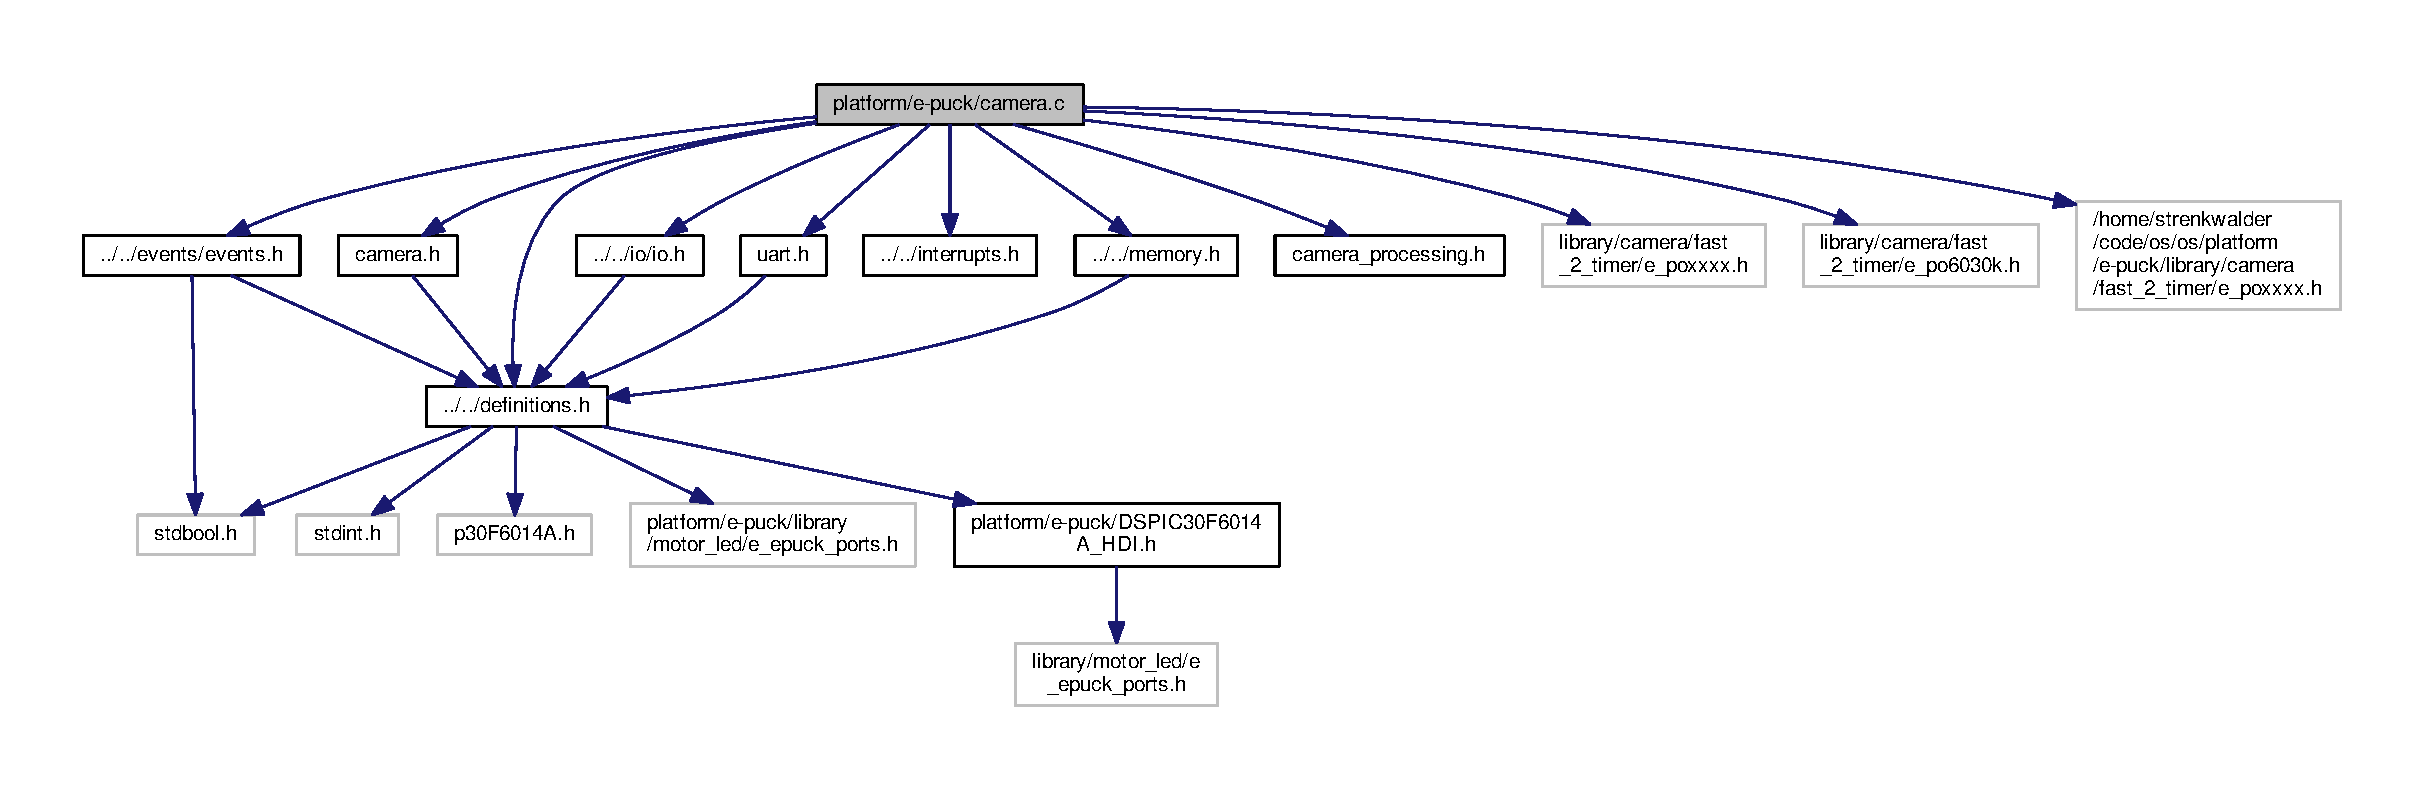
\includegraphics[width=350pt]{d8/d4a/camera_8c__incl}
\end{center}
\end{figure}
\subsection*{Macros}
\begin{DoxyCompactItemize}
\item 
\#define \hyperlink{camera_8c_af193f69a079134ae165cc495b9b62d70}{F\+R\+A\+M\+E\+\_\+\+W\+I\+D\+T\+H}~10
\item 
\#define \hyperlink{camera_8c_a915e7581e140dd2d625fa1cfca365100}{F\+R\+A\+M\+E\+\_\+\+H\+E\+I\+G\+H\+T}~10
\item 
\#define \hyperlink{camera_8c_a823cb7ece14931bb4bf0c7f7311c5c28}{C\+A\+M\+E\+R\+A\+\_\+\+I2\+C\+\_\+\+A\+D\+D\+R\+E\+S\+S}~0x\+D\+C
\item 
\#define \hyperlink{camera_8c_a4c82e201d70da8303a62acd73cbdc9bd}{R\+E\+D\+\_\+\+M\+A\+X}~0x0\+C1\+C
\item 
\#define \hyperlink{camera_8c_afb23383e91ea123e15950b4913bbddc3}{G\+R\+E\+E\+N\+\_\+\+M\+A\+X}~0x189\+C
\item 
\#define \hyperlink{camera_8c_a0651083fdccdfbc5316913c1e73ffd5c}{B\+L\+U\+E\+\_\+\+M\+A\+X}~0x0\+C1\+C
\item 
\#define \hyperlink{camera_8c_acb89fd13fb5b608e0e85a5e476426daa}{R\+E\+D\+\_\+\+T\+H\+R\+E\+S\+H\+O\+L\+D}~0x060\+E
\item 
\#define \hyperlink{camera_8c_a8c258dc6a9038217693e2ca038166582}{G\+R\+E\+E\+N\+\_\+\+T\+H\+R\+E\+S\+H\+O\+L\+D}~0x0\+E4\+E
\item 
\#define \hyperlink{camera_8c_a350f6474fadea2a322a8743a23a87a4e}{B\+L\+U\+E\+\_\+\+T\+H\+R\+E\+S\+H\+O\+L\+D}~0x060\+E
\item 
\#define \hyperlink{camera_8c_ad2cc26b8da12f6603455f84312aa649b}{C\+A\+M\+\_\+\+W\+I\+D\+T\+H}~160
\item 
\#define \hyperlink{camera_8c_ac88d2707293a4af9e155d57e3651162e}{C\+A\+M\+\_\+\+H\+E\+I\+G\+H\+T}~160
\item 
\#define \hyperlink{camera_8c_a8a26078945b82dbf66c0efc3ba627f64}{C\+A\+M\+\_\+\+Z\+O\+O\+M\+\_\+\+X}~8
\item 
\#define \hyperlink{camera_8c_ae584e2494887491a5b7ac09d50a2bddd}{C\+A\+M\+\_\+\+Z\+O\+O\+M\+\_\+\+Y}~8
\item 
\#define \hyperlink{camera_8c_ad704d271abcf09d75aa90b8e8ebb798b}{C\+A\+M\+\_\+\+W\+\_\+\+S\+I\+Z\+E}~20
\item 
\#define \hyperlink{camera_8c_a87f6f0d62673c8b80d55cb254fdaa132}{C\+A\+M\+\_\+\+H\+\_\+\+S\+I\+Z\+E}~20
\item 
\#define \hyperlink{camera_8c_ac1d329efbf5bd63d23e1c623104650a7}{C\+P\+\_\+\+W\+I}~120
\item 
\#define \hyperlink{camera_8c_a9f6f5c8760a079b52078c259212255a3}{C\+P\+\_\+\+R\+I}~80
\item 
\#define \hyperlink{camera_8c_a031d522e9dc797514743213855bee6c9}{C\+P\+\_\+\+G\+I}~80
\item 
\#define \hyperlink{camera_8c_af0acaf3f612c4f6bd5635ff85173b162}{C\+P\+\_\+\+B\+I}~100
\item 
\#define \hyperlink{camera_8c_a8465aecf447b8b92461390e7286ccf48}{C\+O\+L\+O\+U\+R\+\_\+\+T\+H\+R\+E\+S\+H\+O\+L\+D}~766
\end{DoxyCompactItemize}
\subsection*{Functions}
\begin{DoxyCompactItemize}
\item 
void \hyperlink{camera_8c_afc26ad67d7464976b99f5d31f0cc8d38}{Sys\+\_\+\+Process\+\_\+new\+Pixel} (void)
\item 
void \hyperlink{camera_8c_a6db668cb750396e4d0e97752819b1435}{Sys\+\_\+\+Process\+\_\+new\+Line} (void)
\item 
void \hyperlink{camera_8c_ad3061abed97325211e62ade8180f8543}{Sys\+\_\+\+Process\+\_\+new\+Frame} (void)
\item 
void \hyperlink{camera_8c_a559013ac1bda7cdf1b2518bacd32e0e7}{Sys\+\_\+\+Camera\+\_\+\+Pre\+Processor} (void)
\item 
void \hyperlink{camera_8c_a1721a394f7a3d8a2222d979415515d3c}{Sys\+\_\+\+Init\+\_\+\+Camera} ()
\item 
void \hyperlink{camera_8c_acaf0de6115b47aae7870878ba03cf8c4}{Sys\+\_\+\+Start\+\_\+\+Camera} ()
\item 
void \hyperlink{camera_8c_ac93ec56d124a0811e638208ad64ed14c}{Sys\+\_\+\+Set\+\_\+\+Preprocessing} (\hyperlink{camera_8h_ac43fbb39015129f2bb24fecb1d7b33b7}{p\+Camera\+Pre\+Processor} func)
\end{DoxyCompactItemize}


\subsection{Detailed Description}
This file includes functions to process data retrieved by a camera. 

\begin{DoxyAuthor}{Author}
Stefan M. Trenkwalder \href{mailto:s.trenkwalder@openswarm.org}{\tt s.\+trenkwalder@openswarm.\+org} 

Yuri Kaszubowski Lopes \href{mailto:yurikazuba@gmail.com}{\tt yurikazuba@gmail.\+com}
\end{DoxyAuthor}
\begin{DoxyVersion}{Version}
1.\+0
\end{DoxyVersion}
\begin{DoxyDate}{Date}
27 August 2015
\end{DoxyDate}
\begin{DoxyCopyright}{Copyright}
adapted Free\+B\+S\+D License (see \href{http://openswarm.org/license}{\tt http\+://openswarm.\+org/license})
\end{DoxyCopyright}
\begin{DoxyRefDesc}{Todo}
\item[\hyperlink{todo__todo000001}{Todo}]The used functions from the e-\/puck library are very time and computational intensive. These function can be rewritten to decrease the processing load. \end{DoxyRefDesc}


\subsection{Macro Definition Documentation}
\hypertarget{camera_8c_a0651083fdccdfbc5316913c1e73ffd5c}{}\index{camera.\+c@{camera.\+c}!B\+L\+U\+E\+\_\+\+M\+A\+X@{B\+L\+U\+E\+\_\+\+M\+A\+X}}
\index{B\+L\+U\+E\+\_\+\+M\+A\+X@{B\+L\+U\+E\+\_\+\+M\+A\+X}!camera.\+c@{camera.\+c}}
\subsubsection[{B\+L\+U\+E\+\_\+\+M\+A\+X}]{\setlength{\rightskip}{0pt plus 5cm}\#define B\+L\+U\+E\+\_\+\+M\+A\+X~0x0\+C1\+C}\label{camera_8c_a0651083fdccdfbc5316913c1e73ffd5c}
maximum value for received blue 

Definition at line 44 of file camera.\+c.

\hypertarget{camera_8c_a350f6474fadea2a322a8743a23a87a4e}{}\index{camera.\+c@{camera.\+c}!B\+L\+U\+E\+\_\+\+T\+H\+R\+E\+S\+H\+O\+L\+D@{B\+L\+U\+E\+\_\+\+T\+H\+R\+E\+S\+H\+O\+L\+D}}
\index{B\+L\+U\+E\+\_\+\+T\+H\+R\+E\+S\+H\+O\+L\+D@{B\+L\+U\+E\+\_\+\+T\+H\+R\+E\+S\+H\+O\+L\+D}!camera.\+c@{camera.\+c}}
\subsubsection[{B\+L\+U\+E\+\_\+\+T\+H\+R\+E\+S\+H\+O\+L\+D}]{\setlength{\rightskip}{0pt plus 5cm}\#define B\+L\+U\+E\+\_\+\+T\+H\+R\+E\+S\+H\+O\+L\+D~0x060\+E}\label{camera_8c_a350f6474fadea2a322a8743a23a87a4e}
threshold value for received blue 

Definition at line 47 of file camera.\+c.

\hypertarget{camera_8c_a87f6f0d62673c8b80d55cb254fdaa132}{}\index{camera.\+c@{camera.\+c}!C\+A\+M\+\_\+\+H\+\_\+\+S\+I\+Z\+E@{C\+A\+M\+\_\+\+H\+\_\+\+S\+I\+Z\+E}}
\index{C\+A\+M\+\_\+\+H\+\_\+\+S\+I\+Z\+E@{C\+A\+M\+\_\+\+H\+\_\+\+S\+I\+Z\+E}!camera.\+c@{camera.\+c}}
\subsubsection[{C\+A\+M\+\_\+\+H\+\_\+\+S\+I\+Z\+E}]{\setlength{\rightskip}{0pt plus 5cm}\#define C\+A\+M\+\_\+\+H\+\_\+\+S\+I\+Z\+E~20}\label{camera_8c_a87f6f0d62673c8b80d55cb254fdaa132}
post scale height frame 

Definition at line 88 of file camera.\+c.

\hypertarget{camera_8c_ac88d2707293a4af9e155d57e3651162e}{}\index{camera.\+c@{camera.\+c}!C\+A\+M\+\_\+\+H\+E\+I\+G\+H\+T@{C\+A\+M\+\_\+\+H\+E\+I\+G\+H\+T}}
\index{C\+A\+M\+\_\+\+H\+E\+I\+G\+H\+T@{C\+A\+M\+\_\+\+H\+E\+I\+G\+H\+T}!camera.\+c@{camera.\+c}}
\subsubsection[{C\+A\+M\+\_\+\+H\+E\+I\+G\+H\+T}]{\setlength{\rightskip}{0pt plus 5cm}\#define C\+A\+M\+\_\+\+H\+E\+I\+G\+H\+T~160}\label{camera_8c_ac88d2707293a4af9e155d57e3651162e}
height of the camera input frame 

Definition at line 84 of file camera.\+c.

\hypertarget{camera_8c_ad704d271abcf09d75aa90b8e8ebb798b}{}\index{camera.\+c@{camera.\+c}!C\+A\+M\+\_\+\+W\+\_\+\+S\+I\+Z\+E@{C\+A\+M\+\_\+\+W\+\_\+\+S\+I\+Z\+E}}
\index{C\+A\+M\+\_\+\+W\+\_\+\+S\+I\+Z\+E@{C\+A\+M\+\_\+\+W\+\_\+\+S\+I\+Z\+E}!camera.\+c@{camera.\+c}}
\subsubsection[{C\+A\+M\+\_\+\+W\+\_\+\+S\+I\+Z\+E}]{\setlength{\rightskip}{0pt plus 5cm}\#define C\+A\+M\+\_\+\+W\+\_\+\+S\+I\+Z\+E~20}\label{camera_8c_ad704d271abcf09d75aa90b8e8ebb798b}
post scale width frame 

Definition at line 87 of file camera.\+c.

\hypertarget{camera_8c_ad2cc26b8da12f6603455f84312aa649b}{}\index{camera.\+c@{camera.\+c}!C\+A\+M\+\_\+\+W\+I\+D\+T\+H@{C\+A\+M\+\_\+\+W\+I\+D\+T\+H}}
\index{C\+A\+M\+\_\+\+W\+I\+D\+T\+H@{C\+A\+M\+\_\+\+W\+I\+D\+T\+H}!camera.\+c@{camera.\+c}}
\subsubsection[{C\+A\+M\+\_\+\+W\+I\+D\+T\+H}]{\setlength{\rightskip}{0pt plus 5cm}\#define C\+A\+M\+\_\+\+W\+I\+D\+T\+H~160}\label{camera_8c_ad2cc26b8da12f6603455f84312aa649b}
Initialises the I/\+O Management

This function initialises the I/\+O Timer and therefore the I/\+O Management.

param void return void

inline void Sys\+\_\+\+Write\+\_\+to\+\_\+\+Camera(uint8 address, uint8$\ast$ data, uint16 length)\{ uint8 $\ast$i2c\+\_\+data = (uint8 $\ast$) Sys\+\_\+\+Malloc(length+1);

i2c\+\_\+data\mbox{[}0\mbox{]} = address;

Sys\+\_\+\+Memcpy(data, i2c\+\_\+data+1,length);

Sys\+\_\+\+I2\+C\+\_\+\+Sent\+Bytes(C\+A\+M\+E\+R\+A\+\_\+\+I2\+C\+\_\+\+A\+D\+D\+R\+E\+S\+S, i2c\+\_\+data, length+1); \}width of the camera input frame 

Definition at line 83 of file camera.\+c.

\hypertarget{camera_8c_a8a26078945b82dbf66c0efc3ba627f64}{}\index{camera.\+c@{camera.\+c}!C\+A\+M\+\_\+\+Z\+O\+O\+M\+\_\+\+X@{C\+A\+M\+\_\+\+Z\+O\+O\+M\+\_\+\+X}}
\index{C\+A\+M\+\_\+\+Z\+O\+O\+M\+\_\+\+X@{C\+A\+M\+\_\+\+Z\+O\+O\+M\+\_\+\+X}!camera.\+c@{camera.\+c}}
\subsubsection[{C\+A\+M\+\_\+\+Z\+O\+O\+M\+\_\+\+X}]{\setlength{\rightskip}{0pt plus 5cm}\#define C\+A\+M\+\_\+\+Z\+O\+O\+M\+\_\+\+X~8}\label{camera_8c_a8a26078945b82dbf66c0efc3ba627f64}
zoom factor to scale the frame 

Definition at line 85 of file camera.\+c.

\hypertarget{camera_8c_ae584e2494887491a5b7ac09d50a2bddd}{}\index{camera.\+c@{camera.\+c}!C\+A\+M\+\_\+\+Z\+O\+O\+M\+\_\+\+Y@{C\+A\+M\+\_\+\+Z\+O\+O\+M\+\_\+\+Y}}
\index{C\+A\+M\+\_\+\+Z\+O\+O\+M\+\_\+\+Y@{C\+A\+M\+\_\+\+Z\+O\+O\+M\+\_\+\+Y}!camera.\+c@{camera.\+c}}
\subsubsection[{C\+A\+M\+\_\+\+Z\+O\+O\+M\+\_\+\+Y}]{\setlength{\rightskip}{0pt plus 5cm}\#define C\+A\+M\+\_\+\+Z\+O\+O\+M\+\_\+\+Y~8}\label{camera_8c_ae584e2494887491a5b7ac09d50a2bddd}
zoom factor to scale the frame 

Definition at line 86 of file camera.\+c.

\hypertarget{camera_8c_a823cb7ece14931bb4bf0c7f7311c5c28}{}\index{camera.\+c@{camera.\+c}!C\+A\+M\+E\+R\+A\+\_\+\+I2\+C\+\_\+\+A\+D\+D\+R\+E\+S\+S@{C\+A\+M\+E\+R\+A\+\_\+\+I2\+C\+\_\+\+A\+D\+D\+R\+E\+S\+S}}
\index{C\+A\+M\+E\+R\+A\+\_\+\+I2\+C\+\_\+\+A\+D\+D\+R\+E\+S\+S@{C\+A\+M\+E\+R\+A\+\_\+\+I2\+C\+\_\+\+A\+D\+D\+R\+E\+S\+S}!camera.\+c@{camera.\+c}}
\subsubsection[{C\+A\+M\+E\+R\+A\+\_\+\+I2\+C\+\_\+\+A\+D\+D\+R\+E\+S\+S}]{\setlength{\rightskip}{0pt plus 5cm}\#define C\+A\+M\+E\+R\+A\+\_\+\+I2\+C\+\_\+\+A\+D\+D\+R\+E\+S\+S~0x\+D\+C}\label{camera_8c_a823cb7ece14931bb4bf0c7f7311c5c28}
I2\+C address of the camera 

Definition at line 40 of file camera.\+c.

\hypertarget{camera_8c_a8465aecf447b8b92461390e7286ccf48}{}\index{camera.\+c@{camera.\+c}!C\+O\+L\+O\+U\+R\+\_\+\+T\+H\+R\+E\+S\+H\+O\+L\+D@{C\+O\+L\+O\+U\+R\+\_\+\+T\+H\+R\+E\+S\+H\+O\+L\+D}}
\index{C\+O\+L\+O\+U\+R\+\_\+\+T\+H\+R\+E\+S\+H\+O\+L\+D@{C\+O\+L\+O\+U\+R\+\_\+\+T\+H\+R\+E\+S\+H\+O\+L\+D}!camera.\+c@{camera.\+c}}
\subsubsection[{C\+O\+L\+O\+U\+R\+\_\+\+T\+H\+R\+E\+S\+H\+O\+L\+D}]{\setlength{\rightskip}{0pt plus 5cm}\#define C\+O\+L\+O\+U\+R\+\_\+\+T\+H\+R\+E\+S\+H\+O\+L\+D~766}\label{camera_8c_a8465aecf447b8b92461390e7286ccf48}
threshold to decide if a colour pixel has been measured 

Definition at line 540 of file camera.\+c.

\hypertarget{camera_8c_af0acaf3f612c4f6bd5635ff85173b162}{}\index{camera.\+c@{camera.\+c}!C\+P\+\_\+\+B\+I@{C\+P\+\_\+\+B\+I}}
\index{C\+P\+\_\+\+B\+I@{C\+P\+\_\+\+B\+I}!camera.\+c@{camera.\+c}}
\subsubsection[{C\+P\+\_\+\+B\+I}]{\setlength{\rightskip}{0pt plus 5cm}\#define C\+P\+\_\+\+B\+I~100}\label{camera_8c_af0acaf3f612c4f6bd5635ff85173b162}
blue factor to process and calibrate the camera 

Definition at line 539 of file camera.\+c.

\hypertarget{camera_8c_a031d522e9dc797514743213855bee6c9}{}\index{camera.\+c@{camera.\+c}!C\+P\+\_\+\+G\+I@{C\+P\+\_\+\+G\+I}}
\index{C\+P\+\_\+\+G\+I@{C\+P\+\_\+\+G\+I}!camera.\+c@{camera.\+c}}
\subsubsection[{C\+P\+\_\+\+G\+I}]{\setlength{\rightskip}{0pt plus 5cm}\#define C\+P\+\_\+\+G\+I~80}\label{camera_8c_a031d522e9dc797514743213855bee6c9}
green factor to process and calibrate the camera 

Definition at line 538 of file camera.\+c.

\hypertarget{camera_8c_a9f6f5c8760a079b52078c259212255a3}{}\index{camera.\+c@{camera.\+c}!C\+P\+\_\+\+R\+I@{C\+P\+\_\+\+R\+I}}
\index{C\+P\+\_\+\+R\+I@{C\+P\+\_\+\+R\+I}!camera.\+c@{camera.\+c}}
\subsubsection[{C\+P\+\_\+\+R\+I}]{\setlength{\rightskip}{0pt plus 5cm}\#define C\+P\+\_\+\+R\+I~80}\label{camera_8c_a9f6f5c8760a079b52078c259212255a3}
red factor to process and calibrate the camera 

Definition at line 537 of file camera.\+c.

\hypertarget{camera_8c_ac1d329efbf5bd63d23e1c623104650a7}{}\index{camera.\+c@{camera.\+c}!C\+P\+\_\+\+W\+I@{C\+P\+\_\+\+W\+I}}
\index{C\+P\+\_\+\+W\+I@{C\+P\+\_\+\+W\+I}!camera.\+c@{camera.\+c}}
\subsubsection[{C\+P\+\_\+\+W\+I}]{\setlength{\rightskip}{0pt plus 5cm}\#define C\+P\+\_\+\+W\+I~120}\label{camera_8c_ac1d329efbf5bd63d23e1c623104650a7}
whitness factor to process and calibrate the camera 

Definition at line 536 of file camera.\+c.

\hypertarget{camera_8c_a915e7581e140dd2d625fa1cfca365100}{}\index{camera.\+c@{camera.\+c}!F\+R\+A\+M\+E\+\_\+\+H\+E\+I\+G\+H\+T@{F\+R\+A\+M\+E\+\_\+\+H\+E\+I\+G\+H\+T}}
\index{F\+R\+A\+M\+E\+\_\+\+H\+E\+I\+G\+H\+T@{F\+R\+A\+M\+E\+\_\+\+H\+E\+I\+G\+H\+T}!camera.\+c@{camera.\+c}}
\subsubsection[{F\+R\+A\+M\+E\+\_\+\+H\+E\+I\+G\+H\+T}]{\setlength{\rightskip}{0pt plus 5cm}\#define F\+R\+A\+M\+E\+\_\+\+H\+E\+I\+G\+H\+T~10}\label{camera_8c_a915e7581e140dd2d625fa1cfca365100}
Height of the subframe of the image 

Definition at line 39 of file camera.\+c.

\hypertarget{camera_8c_af193f69a079134ae165cc495b9b62d70}{}\index{camera.\+c@{camera.\+c}!F\+R\+A\+M\+E\+\_\+\+W\+I\+D\+T\+H@{F\+R\+A\+M\+E\+\_\+\+W\+I\+D\+T\+H}}
\index{F\+R\+A\+M\+E\+\_\+\+W\+I\+D\+T\+H@{F\+R\+A\+M\+E\+\_\+\+W\+I\+D\+T\+H}!camera.\+c@{camera.\+c}}
\subsubsection[{F\+R\+A\+M\+E\+\_\+\+W\+I\+D\+T\+H}]{\setlength{\rightskip}{0pt plus 5cm}\#define F\+R\+A\+M\+E\+\_\+\+W\+I\+D\+T\+H~10}\label{camera_8c_af193f69a079134ae165cc495b9b62d70}
Width of the subframe of the image 

Definition at line 38 of file camera.\+c.

\hypertarget{camera_8c_afb23383e91ea123e15950b4913bbddc3}{}\index{camera.\+c@{camera.\+c}!G\+R\+E\+E\+N\+\_\+\+M\+A\+X@{G\+R\+E\+E\+N\+\_\+\+M\+A\+X}}
\index{G\+R\+E\+E\+N\+\_\+\+M\+A\+X@{G\+R\+E\+E\+N\+\_\+\+M\+A\+X}!camera.\+c@{camera.\+c}}
\subsubsection[{G\+R\+E\+E\+N\+\_\+\+M\+A\+X}]{\setlength{\rightskip}{0pt plus 5cm}\#define G\+R\+E\+E\+N\+\_\+\+M\+A\+X~0x189\+C}\label{camera_8c_afb23383e91ea123e15950b4913bbddc3}
maximum value for received green 

Definition at line 43 of file camera.\+c.

\hypertarget{camera_8c_a8c258dc6a9038217693e2ca038166582}{}\index{camera.\+c@{camera.\+c}!G\+R\+E\+E\+N\+\_\+\+T\+H\+R\+E\+S\+H\+O\+L\+D@{G\+R\+E\+E\+N\+\_\+\+T\+H\+R\+E\+S\+H\+O\+L\+D}}
\index{G\+R\+E\+E\+N\+\_\+\+T\+H\+R\+E\+S\+H\+O\+L\+D@{G\+R\+E\+E\+N\+\_\+\+T\+H\+R\+E\+S\+H\+O\+L\+D}!camera.\+c@{camera.\+c}}
\subsubsection[{G\+R\+E\+E\+N\+\_\+\+T\+H\+R\+E\+S\+H\+O\+L\+D}]{\setlength{\rightskip}{0pt plus 5cm}\#define G\+R\+E\+E\+N\+\_\+\+T\+H\+R\+E\+S\+H\+O\+L\+D~0x0\+E4\+E}\label{camera_8c_a8c258dc6a9038217693e2ca038166582}
threshold value for received green 

Definition at line 46 of file camera.\+c.

\hypertarget{camera_8c_a4c82e201d70da8303a62acd73cbdc9bd}{}\index{camera.\+c@{camera.\+c}!R\+E\+D\+\_\+\+M\+A\+X@{R\+E\+D\+\_\+\+M\+A\+X}}
\index{R\+E\+D\+\_\+\+M\+A\+X@{R\+E\+D\+\_\+\+M\+A\+X}!camera.\+c@{camera.\+c}}
\subsubsection[{R\+E\+D\+\_\+\+M\+A\+X}]{\setlength{\rightskip}{0pt plus 5cm}\#define R\+E\+D\+\_\+\+M\+A\+X~0x0\+C1\+C}\label{camera_8c_a4c82e201d70da8303a62acd73cbdc9bd}
maximum value for received red 

Definition at line 42 of file camera.\+c.

\hypertarget{camera_8c_acb89fd13fb5b608e0e85a5e476426daa}{}\index{camera.\+c@{camera.\+c}!R\+E\+D\+\_\+\+T\+H\+R\+E\+S\+H\+O\+L\+D@{R\+E\+D\+\_\+\+T\+H\+R\+E\+S\+H\+O\+L\+D}}
\index{R\+E\+D\+\_\+\+T\+H\+R\+E\+S\+H\+O\+L\+D@{R\+E\+D\+\_\+\+T\+H\+R\+E\+S\+H\+O\+L\+D}!camera.\+c@{camera.\+c}}
\subsubsection[{R\+E\+D\+\_\+\+T\+H\+R\+E\+S\+H\+O\+L\+D}]{\setlength{\rightskip}{0pt plus 5cm}\#define R\+E\+D\+\_\+\+T\+H\+R\+E\+S\+H\+O\+L\+D~0x060\+E}\label{camera_8c_acb89fd13fb5b608e0e85a5e476426daa}
threshold value for received red 

Definition at line 45 of file camera.\+c.



\subsection{Function Documentation}
\hypertarget{camera_8c_a559013ac1bda7cdf1b2518bacd32e0e7}{}\index{camera.\+c@{camera.\+c}!Sys\+\_\+\+Camera\+\_\+\+Pre\+Processor@{Sys\+\_\+\+Camera\+\_\+\+Pre\+Processor}}
\index{Sys\+\_\+\+Camera\+\_\+\+Pre\+Processor@{Sys\+\_\+\+Camera\+\_\+\+Pre\+Processor}!camera.\+c@{camera.\+c}}
\subsubsection[{Sys\+\_\+\+Camera\+\_\+\+Pre\+Processor}]{\setlength{\rightskip}{0pt plus 5cm}void Sys\+\_\+\+Camera\+\_\+\+Pre\+Processor (
\begin{DoxyParamCaption}
\item[{void}]{}
\end{DoxyParamCaption}
)}\label{camera_8c_a559013ac1bda7cdf1b2518bacd32e0e7}
processes an incoming camera frame and emits events according to used algorithm

This function processes an incoming camera frame and emits events according to used algorithm.

\begin{DoxyRefDesc}{Todo}
\item[\hyperlink{todo__todo000004}{Todo}]rewrite the camera to computational less intensive functions\end{DoxyRefDesc}


Definition at line 551 of file camera.\+c.

\hypertarget{camera_8c_a1721a394f7a3d8a2222d979415515d3c}{}\index{camera.\+c@{camera.\+c}!Sys\+\_\+\+Init\+\_\+\+Camera@{Sys\+\_\+\+Init\+\_\+\+Camera}}
\index{Sys\+\_\+\+Init\+\_\+\+Camera@{Sys\+\_\+\+Init\+\_\+\+Camera}!camera.\+c@{camera.\+c}}
\subsubsection[{Sys\+\_\+\+Init\+\_\+\+Camera}]{\setlength{\rightskip}{0pt plus 5cm}void Sys\+\_\+\+Init\+\_\+\+Camera (
\begin{DoxyParamCaption}
\item[{void}]{}
\end{DoxyParamCaption}
)}\label{camera_8c_a1721a394f7a3d8a2222d979415515d3c}
Initialises the Camera

This function initialises the camera using e-\/puck library from Subversion at svn\+://svn.gna.\+org/svn/e-\/puck/trunk

\begin{DoxyRefDesc}{Todo}
\item[\hyperlink{todo__todo000002}{Todo}]rewrite the camera to computational less intensive functions\end{DoxyRefDesc}


Definition at line 99 of file camera.\+c.

\hypertarget{camera_8c_ad3061abed97325211e62ade8180f8543}{}\index{camera.\+c@{camera.\+c}!Sys\+\_\+\+Process\+\_\+new\+Frame@{Sys\+\_\+\+Process\+\_\+new\+Frame}}
\index{Sys\+\_\+\+Process\+\_\+new\+Frame@{Sys\+\_\+\+Process\+\_\+new\+Frame}!camera.\+c@{camera.\+c}}
\subsubsection[{Sys\+\_\+\+Process\+\_\+new\+Frame}]{\setlength{\rightskip}{0pt plus 5cm}void Sys\+\_\+\+Process\+\_\+new\+Frame (
\begin{DoxyParamCaption}
\item[{void}]{}
\end{DoxyParamCaption}
)\hspace{0.3cm}{\ttfamily [inline]}}\label{camera_8c_ad3061abed97325211e62ade8180f8543}
\hypertarget{camera_8c_a6db668cb750396e4d0e97752819b1435}{}\index{camera.\+c@{camera.\+c}!Sys\+\_\+\+Process\+\_\+new\+Line@{Sys\+\_\+\+Process\+\_\+new\+Line}}
\index{Sys\+\_\+\+Process\+\_\+new\+Line@{Sys\+\_\+\+Process\+\_\+new\+Line}!camera.\+c@{camera.\+c}}
\subsubsection[{Sys\+\_\+\+Process\+\_\+new\+Line}]{\setlength{\rightskip}{0pt plus 5cm}void Sys\+\_\+\+Process\+\_\+new\+Line (
\begin{DoxyParamCaption}
\item[{void}]{}
\end{DoxyParamCaption}
)\hspace{0.3cm}{\ttfamily [inline]}}\label{camera_8c_a6db668cb750396e4d0e97752819b1435}
\hypertarget{camera_8c_afc26ad67d7464976b99f5d31f0cc8d38}{}\index{camera.\+c@{camera.\+c}!Sys\+\_\+\+Process\+\_\+new\+Pixel@{Sys\+\_\+\+Process\+\_\+new\+Pixel}}
\index{Sys\+\_\+\+Process\+\_\+new\+Pixel@{Sys\+\_\+\+Process\+\_\+new\+Pixel}!camera.\+c@{camera.\+c}}
\subsubsection[{Sys\+\_\+\+Process\+\_\+new\+Pixel}]{\setlength{\rightskip}{0pt plus 5cm}void Sys\+\_\+\+Process\+\_\+new\+Pixel (
\begin{DoxyParamCaption}
\item[{void}]{}
\end{DoxyParamCaption}
)\hspace{0.3cm}{\ttfamily [inline]}}\label{camera_8c_afc26ad67d7464976b99f5d31f0cc8d38}
\hypertarget{camera_8c_ac93ec56d124a0811e638208ad64ed14c}{}\index{camera.\+c@{camera.\+c}!Sys\+\_\+\+Set\+\_\+\+Preprocessing@{Sys\+\_\+\+Set\+\_\+\+Preprocessing}}
\index{Sys\+\_\+\+Set\+\_\+\+Preprocessing@{Sys\+\_\+\+Set\+\_\+\+Preprocessing}!camera.\+c@{camera.\+c}}
\subsubsection[{Sys\+\_\+\+Set\+\_\+\+Preprocessing}]{\setlength{\rightskip}{0pt plus 5cm}void Sys\+\_\+\+Set\+\_\+\+Preprocessing (
\begin{DoxyParamCaption}
\item[{{\bf p\+Camera\+Pre\+Processor}}]{func}
\end{DoxyParamCaption}
)}\label{camera_8c_ac93ec56d124a0811e638208ad64ed14c}
Defines a preprocessor callback functions.

Defines a preprocessor callback functions to process the frame.


\begin{DoxyParams}[1]{Parameters}
\mbox{\tt in}  & {\em func} & camera preprocessor which computes events out of the raw image \\
\hline
\end{DoxyParams}


Definition at line 319 of file camera.\+c.

\hypertarget{camera_8c_acaf0de6115b47aae7870878ba03cf8c4}{}\index{camera.\+c@{camera.\+c}!Sys\+\_\+\+Start\+\_\+\+Camera@{Sys\+\_\+\+Start\+\_\+\+Camera}}
\index{Sys\+\_\+\+Start\+\_\+\+Camera@{Sys\+\_\+\+Start\+\_\+\+Camera}!camera.\+c@{camera.\+c}}
\subsubsection[{Sys\+\_\+\+Start\+\_\+\+Camera}]{\setlength{\rightskip}{0pt plus 5cm}void Sys\+\_\+\+Start\+\_\+\+Camera (
\begin{DoxyParamCaption}
\item[{void}]{}
\end{DoxyParamCaption}
)}\label{camera_8c_acaf0de6115b47aae7870878ba03cf8c4}
Starts the Camera

This function starts the capturing using e-\/puck library from Subversion at svn\+://svn.gna.\+org/svn/e-\/puck/trunk

\begin{DoxyRefDesc}{Todo}
\item[\hyperlink{todo__todo000003}{Todo}]rewrite the camera to computational less intensive functions\end{DoxyRefDesc}


Definition at line 298 of file camera.\+c.


\hypertarget{camera_8h}{}\section{platform/e-\/puck/camera.h File Reference}
\label{camera_8h}\index{platform/e-\/puck/camera.\+h@{platform/e-\/puck/camera.\+h}}


This file includes functions to process data retrieved by a camera.  


{\ttfamily \#include \char`\"{}../../definitions.\+h\char`\"{}}\\*
Include dependency graph for camera.\+h\+:\nopagebreak
\begin{figure}[H]
\begin{center}
\leavevmode
\includegraphics[width=350pt]{d7/d83/camera_8h__incl}
\end{center}
\end{figure}
This graph shows which files directly or indirectly include this file\+:\nopagebreak
\begin{figure}[H]
\begin{center}
\leavevmode
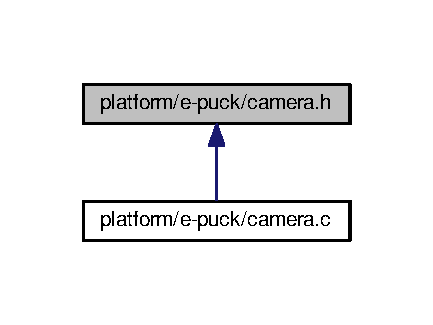
\includegraphics[width=208pt]{d6/d60/camera_8h__dep__incl}
\end{center}
\end{figure}
\subsection*{Data Structures}
\begin{DoxyCompactItemize}
\item 
struct \hyperlink{structsys__rgb__pixel__s}{sys\+\_\+rgb\+\_\+pixel\+\_\+s}
\begin{DoxyCompactList}\small\item\em This bitfield contains the structure of the received pixel of a camera. \end{DoxyCompactList}\end{DoxyCompactItemize}
\subsection*{Macros}
\begin{DoxyCompactItemize}
\item 
\#define \hyperlink{camera_8h_a4f08a1ccf7834bd0d1b8c20c65856a6a}{S\+Y\+S\+\_\+\+M\+A\+X\+\_\+\+R\+E\+D}~0b00011111;
\item 
\#define \hyperlink{camera_8h_ab63ece732ffe256cbb5f3df6f24b721c}{S\+Y\+S\+\_\+\+M\+A\+X\+\_\+\+G\+R\+E\+E\+N}~0b00111111;
\item 
\#define \hyperlink{camera_8h_a80c25ccf9631b085da6582d99d11e094}{S\+Y\+S\+\_\+\+M\+A\+X\+\_\+\+B\+L\+U\+E}~0b00011111;
\end{DoxyCompactItemize}
\subsection*{Typedefs}
\begin{DoxyCompactItemize}
\item 
typedef struct \hyperlink{structsys__rgb__pixel__s}{sys\+\_\+rgb\+\_\+pixel\+\_\+s} \hyperlink{camera_8h_ab3179612ebed45894443a98b02ffb391}{sys\+\_\+rgb}
\begin{DoxyCompactList}\small\item\em This bitfield contains the structure of the received pixel of a camera. \end{DoxyCompactList}\item 
typedef struct \hyperlink{structsys__rgb__pixel__s}{sys\+\_\+rgb\+\_\+pixel\+\_\+s} \hyperlink{camera_8h_a49de3603363bff3140540b40d5fec700}{sys\+\_\+rgb\+\_\+pixel}
\item 
typedef void($\ast$ \hyperlink{camera_8h_ac43fbb39015129f2bb24fecb1d7b33b7}{p\+Camera\+Pre\+Processor}) (\hyperlink{camera_8h_a49de3603363bff3140540b40d5fec700}{sys\+\_\+rgb\+\_\+pixel} $\ast$$\ast$frame, \hyperlink{definitions_8h_a05f6b0ae8f6a6e135b0e290c25fe0e4e}{uint16} width, \hyperlink{definitions_8h_a05f6b0ae8f6a6e135b0e290c25fe0e4e}{uint16} height)
\end{DoxyCompactItemize}
\subsection*{Functions}
\begin{DoxyCompactItemize}
\item 
void \hyperlink{camera_8h_aeefbe8dd86aa2b4588e5e5aa596d41fe}{Sys\+\_\+\+Init\+\_\+\+Camera} (void)
\item 
void \hyperlink{camera_8h_ac44e432642eee885441e01f976e2c969}{Sys\+\_\+\+Start\+\_\+\+Camera} (void)
\item 
void \hyperlink{camera_8h_ac93ec56d124a0811e638208ad64ed14c}{Sys\+\_\+\+Set\+\_\+\+Preprocessing} (\hyperlink{camera_8h_ac43fbb39015129f2bb24fecb1d7b33b7}{p\+Camera\+Pre\+Processor} func)
\item 
\hyperlink{camera_8h_a49de3603363bff3140540b40d5fec700}{sys\+\_\+rgb\+\_\+pixel} $\ast$ \hyperlink{camera_8h_a72c1d6c27d3aeb8399ec41247cc4ba58}{get\+Finished\+Frame} ()
\item 
bool \hyperlink{camera_8h_a1b0543ca3f9389e59135838a3c9cbb23}{is\+New\+Frame\+Available} ()
\end{DoxyCompactItemize}


\subsection{Detailed Description}
This file includes functions to process data retrieved by a camera. 

\begin{DoxyAuthor}{Author}
Stefan M. Trenkwalder \href{mailto:s.trenkwalder@openswarm.org}{\tt s.\+trenkwalder@openswarm.\+org} 
\end{DoxyAuthor}
\begin{DoxyVersion}{Version}
1.\+0
\end{DoxyVersion}
\begin{DoxyDate}{Date}
27 August 2015
\end{DoxyDate}
\begin{DoxyCopyright}{Copyright}
adapted Free\+B\+S\+D License (see \href{http://openswarm.org/license}{\tt http\+://openswarm.\+org/license}) 
\end{DoxyCopyright}


\subsection{Macro Definition Documentation}
\hypertarget{camera_8h_a80c25ccf9631b085da6582d99d11e094}{}\index{camera.\+h@{camera.\+h}!S\+Y\+S\+\_\+\+M\+A\+X\+\_\+\+B\+L\+U\+E@{S\+Y\+S\+\_\+\+M\+A\+X\+\_\+\+B\+L\+U\+E}}
\index{S\+Y\+S\+\_\+\+M\+A\+X\+\_\+\+B\+L\+U\+E@{S\+Y\+S\+\_\+\+M\+A\+X\+\_\+\+B\+L\+U\+E}!camera.\+h@{camera.\+h}}
\subsubsection[{S\+Y\+S\+\_\+\+M\+A\+X\+\_\+\+B\+L\+U\+E}]{\setlength{\rightskip}{0pt plus 5cm}\#define S\+Y\+S\+\_\+\+M\+A\+X\+\_\+\+B\+L\+U\+E~0b00011111;}\label{camera_8h_a80c25ccf9631b085da6582d99d11e094}
blue bits received 

Definition at line 52 of file camera.\+h.

\hypertarget{camera_8h_ab63ece732ffe256cbb5f3df6f24b721c}{}\index{camera.\+h@{camera.\+h}!S\+Y\+S\+\_\+\+M\+A\+X\+\_\+\+G\+R\+E\+E\+N@{S\+Y\+S\+\_\+\+M\+A\+X\+\_\+\+G\+R\+E\+E\+N}}
\index{S\+Y\+S\+\_\+\+M\+A\+X\+\_\+\+G\+R\+E\+E\+N@{S\+Y\+S\+\_\+\+M\+A\+X\+\_\+\+G\+R\+E\+E\+N}!camera.\+h@{camera.\+h}}
\subsubsection[{S\+Y\+S\+\_\+\+M\+A\+X\+\_\+\+G\+R\+E\+E\+N}]{\setlength{\rightskip}{0pt plus 5cm}\#define S\+Y\+S\+\_\+\+M\+A\+X\+\_\+\+G\+R\+E\+E\+N~0b00111111;}\label{camera_8h_ab63ece732ffe256cbb5f3df6f24b721c}
green bits received 

Definition at line 51 of file camera.\+h.

\hypertarget{camera_8h_a4f08a1ccf7834bd0d1b8c20c65856a6a}{}\index{camera.\+h@{camera.\+h}!S\+Y\+S\+\_\+\+M\+A\+X\+\_\+\+R\+E\+D@{S\+Y\+S\+\_\+\+M\+A\+X\+\_\+\+R\+E\+D}}
\index{S\+Y\+S\+\_\+\+M\+A\+X\+\_\+\+R\+E\+D@{S\+Y\+S\+\_\+\+M\+A\+X\+\_\+\+R\+E\+D}!camera.\+h@{camera.\+h}}
\subsubsection[{S\+Y\+S\+\_\+\+M\+A\+X\+\_\+\+R\+E\+D}]{\setlength{\rightskip}{0pt plus 5cm}\#define S\+Y\+S\+\_\+\+M\+A\+X\+\_\+\+R\+E\+D~0b00011111;}\label{camera_8h_a4f08a1ccf7834bd0d1b8c20c65856a6a}
red bits received 

Definition at line 50 of file camera.\+h.



\subsection{Typedef Documentation}
\hypertarget{camera_8h_ac43fbb39015129f2bb24fecb1d7b33b7}{}\index{camera.\+h@{camera.\+h}!p\+Camera\+Pre\+Processor@{p\+Camera\+Pre\+Processor}}
\index{p\+Camera\+Pre\+Processor@{p\+Camera\+Pre\+Processor}!camera.\+h@{camera.\+h}}
\subsubsection[{p\+Camera\+Pre\+Processor}]{\setlength{\rightskip}{0pt plus 5cm}typedef void($\ast$ p\+Camera\+Pre\+Processor) ({\bf sys\+\_\+rgb\+\_\+pixel} $\ast$$\ast$frame, {\bf uint16} width, {\bf uint16} height)}\label{camera_8h_ac43fbb39015129f2bb24fecb1d7b33b7}
pointer to a camera preprocessor 

Definition at line 63 of file camera.\+h.

\hypertarget{camera_8h_ab3179612ebed45894443a98b02ffb391}{}\index{camera.\+h@{camera.\+h}!sys\+\_\+rgb@{sys\+\_\+rgb}}
\index{sys\+\_\+rgb@{sys\+\_\+rgb}!camera.\+h@{camera.\+h}}
\subsubsection[{sys\+\_\+rgb}]{\setlength{\rightskip}{0pt plus 5cm}typedef struct {\bf sys\+\_\+rgb\+\_\+pixel\+\_\+s} {\bf sys\+\_\+rgb}}\label{camera_8h_ab3179612ebed45894443a98b02ffb391}


This bitfield contains the structure of the received pixel of a camera. 

\hypertarget{camera_8h_a49de3603363bff3140540b40d5fec700}{}\index{camera.\+h@{camera.\+h}!sys\+\_\+rgb\+\_\+pixel@{sys\+\_\+rgb\+\_\+pixel}}
\index{sys\+\_\+rgb\+\_\+pixel@{sys\+\_\+rgb\+\_\+pixel}!camera.\+h@{camera.\+h}}
\subsubsection[{sys\+\_\+rgb\+\_\+pixel}]{\setlength{\rightskip}{0pt plus 5cm}typedef struct {\bf sys\+\_\+rgb\+\_\+pixel\+\_\+s}  {\bf sys\+\_\+rgb\+\_\+pixel}}\label{camera_8h_a49de3603363bff3140540b40d5fec700}


\subsection{Function Documentation}
\hypertarget{camera_8h_a72c1d6c27d3aeb8399ec41247cc4ba58}{}\index{camera.\+h@{camera.\+h}!get\+Finished\+Frame@{get\+Finished\+Frame}}
\index{get\+Finished\+Frame@{get\+Finished\+Frame}!camera.\+h@{camera.\+h}}
\subsubsection[{get\+Finished\+Frame}]{\setlength{\rightskip}{0pt plus 5cm}{\bf sys\+\_\+rgb\+\_\+pixel}$\ast$ get\+Finished\+Frame (
\begin{DoxyParamCaption}
{}
\end{DoxyParamCaption}
)}\label{camera_8h_a72c1d6c27d3aeb8399ec41247cc4ba58}
\hypertarget{camera_8h_a1b0543ca3f9389e59135838a3c9cbb23}{}\index{camera.\+h@{camera.\+h}!is\+New\+Frame\+Available@{is\+New\+Frame\+Available}}
\index{is\+New\+Frame\+Available@{is\+New\+Frame\+Available}!camera.\+h@{camera.\+h}}
\subsubsection[{is\+New\+Frame\+Available}]{\setlength{\rightskip}{0pt plus 5cm}bool is\+New\+Frame\+Available (
\begin{DoxyParamCaption}
{}
\end{DoxyParamCaption}
)}\label{camera_8h_a1b0543ca3f9389e59135838a3c9cbb23}
\hypertarget{camera_8h_aeefbe8dd86aa2b4588e5e5aa596d41fe}{}\index{camera.\+h@{camera.\+h}!Sys\+\_\+\+Init\+\_\+\+Camera@{Sys\+\_\+\+Init\+\_\+\+Camera}}
\index{Sys\+\_\+\+Init\+\_\+\+Camera@{Sys\+\_\+\+Init\+\_\+\+Camera}!camera.\+h@{camera.\+h}}
\subsubsection[{Sys\+\_\+\+Init\+\_\+\+Camera}]{\setlength{\rightskip}{0pt plus 5cm}void Sys\+\_\+\+Init\+\_\+\+Camera (
\begin{DoxyParamCaption}
\item[{void}]{}
\end{DoxyParamCaption}
)}\label{camera_8h_aeefbe8dd86aa2b4588e5e5aa596d41fe}
Initialises the Camera

This function initialises the camera using e-\/puck library from Subversion at svn\+://svn.gna.\+org/svn/e-\/puck/trunk

\begin{DoxyRefDesc}{Todo}
\item[\hyperlink{todo__todo000002}{Todo}]rewrite the camera to computational less intensive functions\end{DoxyRefDesc}


Definition at line 99 of file camera.\+c.

\hypertarget{camera_8h_ac93ec56d124a0811e638208ad64ed14c}{}\index{camera.\+h@{camera.\+h}!Sys\+\_\+\+Set\+\_\+\+Preprocessing@{Sys\+\_\+\+Set\+\_\+\+Preprocessing}}
\index{Sys\+\_\+\+Set\+\_\+\+Preprocessing@{Sys\+\_\+\+Set\+\_\+\+Preprocessing}!camera.\+h@{camera.\+h}}
\subsubsection[{Sys\+\_\+\+Set\+\_\+\+Preprocessing}]{\setlength{\rightskip}{0pt plus 5cm}void Sys\+\_\+\+Set\+\_\+\+Preprocessing (
\begin{DoxyParamCaption}
\item[{{\bf p\+Camera\+Pre\+Processor}}]{func}
\end{DoxyParamCaption}
)}\label{camera_8h_ac93ec56d124a0811e638208ad64ed14c}
Defines a preprocessor callback functions.

Defines a preprocessor callback functions to process the frame.


\begin{DoxyParams}[1]{Parameters}
\mbox{\tt in}  & {\em func} & camera preprocessor which computes events out of the raw image \\
\hline
\end{DoxyParams}


Definition at line 319 of file camera.\+c.

\hypertarget{camera_8h_ac44e432642eee885441e01f976e2c969}{}\index{camera.\+h@{camera.\+h}!Sys\+\_\+\+Start\+\_\+\+Camera@{Sys\+\_\+\+Start\+\_\+\+Camera}}
\index{Sys\+\_\+\+Start\+\_\+\+Camera@{Sys\+\_\+\+Start\+\_\+\+Camera}!camera.\+h@{camera.\+h}}
\subsubsection[{Sys\+\_\+\+Start\+\_\+\+Camera}]{\setlength{\rightskip}{0pt plus 5cm}void Sys\+\_\+\+Start\+\_\+\+Camera (
\begin{DoxyParamCaption}
\item[{void}]{}
\end{DoxyParamCaption}
)}\label{camera_8h_ac44e432642eee885441e01f976e2c969}
Starts the Camera

This function starts the capturing using e-\/puck library from Subversion at svn\+://svn.gna.\+org/svn/e-\/puck/trunk

\begin{DoxyRefDesc}{Todo}
\item[\hyperlink{todo__todo000003}{Todo}]rewrite the camera to computational less intensive functions\end{DoxyRefDesc}


Definition at line 298 of file camera.\+c.


\hypertarget{camera__processing_8c}{}\subsection{platform/e-\/puck/camera\+\_\+processing.c File Reference}
\label{camera__processing_8c}\index{platform/e-\/puck/camera\+\_\+processing.\+c@{platform/e-\/puck/camera\+\_\+processing.\+c}}
{\ttfamily \#include \char`\"{}camera\+\_\+processing.\+h\char`\"{}}\\*
{\ttfamily \#include $<$math.\+h$>$}\\*
{\ttfamily \#include $<$stdio.\+h$>$}\\*
Include dependency graph for camera\+\_\+processing.\+c\+:\nopagebreak
\begin{figure}[H]
\begin{center}
\leavevmode
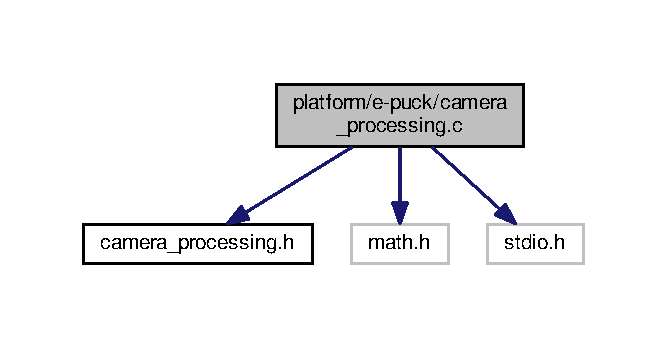
\includegraphics[width=320pt]{d0/dbb/camera__processing_8c__incl}
\end{center}
\end{figure}
\subsubsection*{Macros}
\begin{DoxyCompactItemize}
\item 
\#define \hyperlink{camera__processing_8c_ac1d329efbf5bd63d23e1c623104650a7}{C\+P\+\_\+\+W\+I}~100
\item 
\#define \hyperlink{camera__processing_8c_a423f50937f8bb653d67f6b68049527ea}{C\+P\+\_\+\+W\+G\+B\+\_\+\+I}~80
\item 
\#define \hyperlink{camera__processing_8c_a9f6f5c8760a079b52078c259212255a3}{C\+P\+\_\+\+R\+I}~80
\item 
\#define \hyperlink{camera__processing_8c_a031d522e9dc797514743213855bee6c9}{C\+P\+\_\+\+G\+I}~40
\item 
\#define \hyperlink{camera__processing_8c_af0acaf3f612c4f6bd5635ff85173b162}{C\+P\+\_\+\+B\+I}~100
\item 
\#define \hyperlink{camera__processing_8c_ad683afd109dbb4a0ba3a305695b49095}{C\+B\+P\+\_\+\+W\+I}~16
\item 
\#define \hyperlink{camera__processing_8c_ac8d9040a94f25bd12d6972838d18c99c}{C\+B\+P\+\_\+\+R\+I}~11
\item 
\#define \hyperlink{camera__processing_8c_a88b9154d8df00524dbc91f1f967aacf0}{C\+B\+P\+\_\+\+G\+I}~11
\item 
\#define \hyperlink{camera__processing_8c_ae4272405bfe7895ae551a73eb3e57ce4}{C\+B\+P\+\_\+\+B\+I}~13
\item 
\#define \hyperlink{camera__processing_8c_a1bd13187a78a2c1258be972e24a06ce4}{C\+B\+P\+\_\+\+D\+I}~2
\end{DoxyCompactItemize}
\subsubsection*{Functions}
\begin{DoxyCompactItemize}
\item 
void \hyperlink{camera__processing_8c_a805427a51bfe2cf4d675d7cb479b819b}{convert\+R\+G\+B565\+To\+R\+G\+B888} (unsigned char rgb565\mbox{[}$\,$\mbox{]}, unsigned char rgb888\mbox{[}$\,$\mbox{]})
\item 
void \hyperlink{camera__processing_8c_afd2b8279decc2ab40000170b5506d385}{get\+R\+G\+B565at} (char $\ast$buffer, unsigned char rgb585\mbox{[}$\,$\mbox{]}, int x, int y)
\item 
void \hyperlink{camera__processing_8c_a8cfb72ecb08503eca4d6efc58b9987f2}{get\+R\+G\+B888at} (char $\ast$buffer, unsigned char rgb888\mbox{[}$\,$\mbox{]}, int x, int y)
\item 
char \hyperlink{camera__processing_8c_a8655b5660f79ef090db798451f1ed701}{nearest\+Neighbor\+R\+G\+B} (unsigned char $\ast$rbg888, char flag)
\item 
char \hyperlink{camera__processing_8c_ad921ae36e7f4fb378e1b67c2d1817244}{brushed\+Color\+From\+R\+G\+B565} (unsigned char rgb565\mbox{[}$\,$\mbox{]}, char flag)
\item 
char \hyperlink{camera__processing_8c_a587d4ed6a588eacad21baf2ac5aa1f10}{get\+Brushed\+Color\+At} (char $\ast$buffer, char flag, int x, int y, int w)
\end{DoxyCompactItemize}
\subsubsection*{Variables}
\begin{DoxyCompactItemize}
\item 
const unsigned char \hyperlink{camera__processing_8c_a9eb4d4edc09176b41bb78a120a3dbaf5}{color\+Positions} \mbox{[}8\mbox{]}\mbox{[}4\mbox{]}
\item 
const int \hyperlink{camera__processing_8c_afea30c7dedb8b7deb70d4ab8ec9c8eed}{power\+Tbl} \mbox{[}33\mbox{]} = \{0,1,4,9,16,25,36,49,64,81,100,121,144,169,196,225,256,289,324,361,400,441,484,529,576,625,676,729,784,841,900,961,1024\}
\item 
const unsigned char \hyperlink{camera__processing_8c_ac42b96872bf2f2373b80d1fcb3deaed9}{color\+Brushed\+Positions} \mbox{[}8\mbox{]}\mbox{[}4\mbox{]}
\end{DoxyCompactItemize}


\subsubsection{Detailed Description}
\begin{DoxyAuthor}{Author}
Yuri Kaszubowski Lopes \href{mailto:yurikazuba@gmail.com}{\tt yurikazuba@gmail.\+com} 
\end{DoxyAuthor}
\begin{DoxyVersion}{Version}
1.\+0
\end{DoxyVersion}
\begin{DoxyDate}{Date}
2014 
\end{DoxyDate}


\subsubsection{Macro Definition Documentation}
\hypertarget{camera__processing_8c_ae4272405bfe7895ae551a73eb3e57ce4}{}\index{camera\+\_\+processing.\+c@{camera\+\_\+processing.\+c}!C\+B\+P\+\_\+\+B\+I@{C\+B\+P\+\_\+\+B\+I}}
\index{C\+B\+P\+\_\+\+B\+I@{C\+B\+P\+\_\+\+B\+I}!camera\+\_\+processing.\+c@{camera\+\_\+processing.\+c}}
\paragraph[{C\+B\+P\+\_\+\+B\+I}]{\setlength{\rightskip}{0pt plus 5cm}\#define C\+B\+P\+\_\+\+B\+I~13}\label{camera__processing_8c_ae4272405bfe7895ae551a73eb3e57ce4}


Definition at line 72 of file camera\+\_\+processing.\+c.

\hypertarget{camera__processing_8c_a1bd13187a78a2c1258be972e24a06ce4}{}\index{camera\+\_\+processing.\+c@{camera\+\_\+processing.\+c}!C\+B\+P\+\_\+\+D\+I@{C\+B\+P\+\_\+\+D\+I}}
\index{C\+B\+P\+\_\+\+D\+I@{C\+B\+P\+\_\+\+D\+I}!camera\+\_\+processing.\+c@{camera\+\_\+processing.\+c}}
\paragraph[{C\+B\+P\+\_\+\+D\+I}]{\setlength{\rightskip}{0pt plus 5cm}\#define C\+B\+P\+\_\+\+D\+I~2}\label{camera__processing_8c_a1bd13187a78a2c1258be972e24a06ce4}


Definition at line 73 of file camera\+\_\+processing.\+c.

\hypertarget{camera__processing_8c_a88b9154d8df00524dbc91f1f967aacf0}{}\index{camera\+\_\+processing.\+c@{camera\+\_\+processing.\+c}!C\+B\+P\+\_\+\+G\+I@{C\+B\+P\+\_\+\+G\+I}}
\index{C\+B\+P\+\_\+\+G\+I@{C\+B\+P\+\_\+\+G\+I}!camera\+\_\+processing.\+c@{camera\+\_\+processing.\+c}}
\paragraph[{C\+B\+P\+\_\+\+G\+I}]{\setlength{\rightskip}{0pt plus 5cm}\#define C\+B\+P\+\_\+\+G\+I~11}\label{camera__processing_8c_a88b9154d8df00524dbc91f1f967aacf0}


Definition at line 71 of file camera\+\_\+processing.\+c.

\hypertarget{camera__processing_8c_ac8d9040a94f25bd12d6972838d18c99c}{}\index{camera\+\_\+processing.\+c@{camera\+\_\+processing.\+c}!C\+B\+P\+\_\+\+R\+I@{C\+B\+P\+\_\+\+R\+I}}
\index{C\+B\+P\+\_\+\+R\+I@{C\+B\+P\+\_\+\+R\+I}!camera\+\_\+processing.\+c@{camera\+\_\+processing.\+c}}
\paragraph[{C\+B\+P\+\_\+\+R\+I}]{\setlength{\rightskip}{0pt plus 5cm}\#define C\+B\+P\+\_\+\+R\+I~11}\label{camera__processing_8c_ac8d9040a94f25bd12d6972838d18c99c}


Definition at line 70 of file camera\+\_\+processing.\+c.

\hypertarget{camera__processing_8c_ad683afd109dbb4a0ba3a305695b49095}{}\index{camera\+\_\+processing.\+c@{camera\+\_\+processing.\+c}!C\+B\+P\+\_\+\+W\+I@{C\+B\+P\+\_\+\+W\+I}}
\index{C\+B\+P\+\_\+\+W\+I@{C\+B\+P\+\_\+\+W\+I}!camera\+\_\+processing.\+c@{camera\+\_\+processing.\+c}}
\paragraph[{C\+B\+P\+\_\+\+W\+I}]{\setlength{\rightskip}{0pt plus 5cm}\#define C\+B\+P\+\_\+\+W\+I~16}\label{camera__processing_8c_ad683afd109dbb4a0ba3a305695b49095}


Definition at line 69 of file camera\+\_\+processing.\+c.

\hypertarget{camera__processing_8c_af0acaf3f612c4f6bd5635ff85173b162}{}\index{camera\+\_\+processing.\+c@{camera\+\_\+processing.\+c}!C\+P\+\_\+\+B\+I@{C\+P\+\_\+\+B\+I}}
\index{C\+P\+\_\+\+B\+I@{C\+P\+\_\+\+B\+I}!camera\+\_\+processing.\+c@{camera\+\_\+processing.\+c}}
\paragraph[{C\+P\+\_\+\+B\+I}]{\setlength{\rightskip}{0pt plus 5cm}\#define C\+P\+\_\+\+B\+I~100}\label{camera__processing_8c_af0acaf3f612c4f6bd5635ff85173b162}


Definition at line 36 of file camera\+\_\+processing.\+c.

\hypertarget{camera__processing_8c_a031d522e9dc797514743213855bee6c9}{}\index{camera\+\_\+processing.\+c@{camera\+\_\+processing.\+c}!C\+P\+\_\+\+G\+I@{C\+P\+\_\+\+G\+I}}
\index{C\+P\+\_\+\+G\+I@{C\+P\+\_\+\+G\+I}!camera\+\_\+processing.\+c@{camera\+\_\+processing.\+c}}
\paragraph[{C\+P\+\_\+\+G\+I}]{\setlength{\rightskip}{0pt plus 5cm}\#define C\+P\+\_\+\+G\+I~40}\label{camera__processing_8c_a031d522e9dc797514743213855bee6c9}


Definition at line 35 of file camera\+\_\+processing.\+c.

\hypertarget{camera__processing_8c_a9f6f5c8760a079b52078c259212255a3}{}\index{camera\+\_\+processing.\+c@{camera\+\_\+processing.\+c}!C\+P\+\_\+\+R\+I@{C\+P\+\_\+\+R\+I}}
\index{C\+P\+\_\+\+R\+I@{C\+P\+\_\+\+R\+I}!camera\+\_\+processing.\+c@{camera\+\_\+processing.\+c}}
\paragraph[{C\+P\+\_\+\+R\+I}]{\setlength{\rightskip}{0pt plus 5cm}\#define C\+P\+\_\+\+R\+I~80}\label{camera__processing_8c_a9f6f5c8760a079b52078c259212255a3}


Definition at line 34 of file camera\+\_\+processing.\+c.

\hypertarget{camera__processing_8c_a423f50937f8bb653d67f6b68049527ea}{}\index{camera\+\_\+processing.\+c@{camera\+\_\+processing.\+c}!C\+P\+\_\+\+W\+G\+B\+\_\+\+I@{C\+P\+\_\+\+W\+G\+B\+\_\+\+I}}
\index{C\+P\+\_\+\+W\+G\+B\+\_\+\+I@{C\+P\+\_\+\+W\+G\+B\+\_\+\+I}!camera\+\_\+processing.\+c@{camera\+\_\+processing.\+c}}
\paragraph[{C\+P\+\_\+\+W\+G\+B\+\_\+\+I}]{\setlength{\rightskip}{0pt plus 5cm}\#define C\+P\+\_\+\+W\+G\+B\+\_\+\+I~80}\label{camera__processing_8c_a423f50937f8bb653d67f6b68049527ea}


Definition at line 33 of file camera\+\_\+processing.\+c.

\hypertarget{camera__processing_8c_ac1d329efbf5bd63d23e1c623104650a7}{}\index{camera\+\_\+processing.\+c@{camera\+\_\+processing.\+c}!C\+P\+\_\+\+W\+I@{C\+P\+\_\+\+W\+I}}
\index{C\+P\+\_\+\+W\+I@{C\+P\+\_\+\+W\+I}!camera\+\_\+processing.\+c@{camera\+\_\+processing.\+c}}
\paragraph[{C\+P\+\_\+\+W\+I}]{\setlength{\rightskip}{0pt plus 5cm}\#define C\+P\+\_\+\+W\+I~100}\label{camera__processing_8c_ac1d329efbf5bd63d23e1c623104650a7}


Definition at line 32 of file camera\+\_\+processing.\+c.



\subsubsection{Function Documentation}
\hypertarget{camera__processing_8c_ad921ae36e7f4fb378e1b67c2d1817244}{}\index{camera\+\_\+processing.\+c@{camera\+\_\+processing.\+c}!brushed\+Color\+From\+R\+G\+B565@{brushed\+Color\+From\+R\+G\+B565}}
\index{brushed\+Color\+From\+R\+G\+B565@{brushed\+Color\+From\+R\+G\+B565}!camera\+\_\+processing.\+c@{camera\+\_\+processing.\+c}}
\paragraph[{brushed\+Color\+From\+R\+G\+B565}]{\setlength{\rightskip}{0pt plus 5cm}char brushed\+Color\+From\+R\+G\+B565 (
\begin{DoxyParamCaption}
\item[{unsigned char}]{rgb565\mbox{[}$\,$\mbox{]}, }
\item[{char}]{flag}
\end{DoxyParamCaption}
)}\label{camera__processing_8c_ad921ae36e7f4fb378e1b67c2d1817244}


Definition at line 86 of file camera\+\_\+processing.\+c.

\hypertarget{camera__processing_8c_a805427a51bfe2cf4d675d7cb479b819b}{}\index{camera\+\_\+processing.\+c@{camera\+\_\+processing.\+c}!convert\+R\+G\+B565\+To\+R\+G\+B888@{convert\+R\+G\+B565\+To\+R\+G\+B888}}
\index{convert\+R\+G\+B565\+To\+R\+G\+B888@{convert\+R\+G\+B565\+To\+R\+G\+B888}!camera\+\_\+processing.\+c@{camera\+\_\+processing.\+c}}
\paragraph[{convert\+R\+G\+B565\+To\+R\+G\+B888}]{\setlength{\rightskip}{0pt plus 5cm}void convert\+R\+G\+B565\+To\+R\+G\+B888 (
\begin{DoxyParamCaption}
\item[{unsigned char}]{rgb565\mbox{[}$\,$\mbox{]}, }
\item[{unsigned char}]{rgb888\mbox{[}$\,$\mbox{]}}
\end{DoxyParamCaption}
)}\label{camera__processing_8c_a805427a51bfe2cf4d675d7cb479b819b}


Definition at line 15 of file camera\+\_\+processing.\+c.

\hypertarget{camera__processing_8c_a587d4ed6a588eacad21baf2ac5aa1f10}{}\index{camera\+\_\+processing.\+c@{camera\+\_\+processing.\+c}!get\+Brushed\+Color\+At@{get\+Brushed\+Color\+At}}
\index{get\+Brushed\+Color\+At@{get\+Brushed\+Color\+At}!camera\+\_\+processing.\+c@{camera\+\_\+processing.\+c}}
\paragraph[{get\+Brushed\+Color\+At}]{\setlength{\rightskip}{0pt plus 5cm}char get\+Brushed\+Color\+At (
\begin{DoxyParamCaption}
\item[{char $\ast$}]{buffer, }
\item[{char}]{flag, }
\item[{int}]{x, }
\item[{int}]{y, }
\item[{int}]{w}
\end{DoxyParamCaption}
)}\label{camera__processing_8c_a587d4ed6a588eacad21baf2ac5aa1f10}


Definition at line 109 of file camera\+\_\+processing.\+c.

\hypertarget{camera__processing_8c_afd2b8279decc2ab40000170b5506d385}{}\index{camera\+\_\+processing.\+c@{camera\+\_\+processing.\+c}!get\+R\+G\+B565at@{get\+R\+G\+B565at}}
\index{get\+R\+G\+B565at@{get\+R\+G\+B565at}!camera\+\_\+processing.\+c@{camera\+\_\+processing.\+c}}
\paragraph[{get\+R\+G\+B565at}]{\setlength{\rightskip}{0pt plus 5cm}void get\+R\+G\+B565at (
\begin{DoxyParamCaption}
\item[{char $\ast$}]{buffer, }
\item[{unsigned char}]{rgb585\mbox{[}$\,$\mbox{]}, }
\item[{int}]{x, }
\item[{int}]{y}
\end{DoxyParamCaption}
)}\label{camera__processing_8c_afd2b8279decc2ab40000170b5506d385}


Definition at line 21 of file camera\+\_\+processing.\+c.

\hypertarget{camera__processing_8c_a8cfb72ecb08503eca4d6efc58b9987f2}{}\index{camera\+\_\+processing.\+c@{camera\+\_\+processing.\+c}!get\+R\+G\+B888at@{get\+R\+G\+B888at}}
\index{get\+R\+G\+B888at@{get\+R\+G\+B888at}!camera\+\_\+processing.\+c@{camera\+\_\+processing.\+c}}
\paragraph[{get\+R\+G\+B888at}]{\setlength{\rightskip}{0pt plus 5cm}void get\+R\+G\+B888at (
\begin{DoxyParamCaption}
\item[{char $\ast$}]{buffer, }
\item[{unsigned char}]{rgb888\mbox{[}$\,$\mbox{]}, }
\item[{int}]{x, }
\item[{int}]{y}
\end{DoxyParamCaption}
)}\label{camera__processing_8c_a8cfb72ecb08503eca4d6efc58b9987f2}


Definition at line 26 of file camera\+\_\+processing.\+c.

\hypertarget{camera__processing_8c_a8655b5660f79ef090db798451f1ed701}{}\index{camera\+\_\+processing.\+c@{camera\+\_\+processing.\+c}!nearest\+Neighbor\+R\+G\+B@{nearest\+Neighbor\+R\+G\+B}}
\index{nearest\+Neighbor\+R\+G\+B@{nearest\+Neighbor\+R\+G\+B}!camera\+\_\+processing.\+c@{camera\+\_\+processing.\+c}}
\paragraph[{nearest\+Neighbor\+R\+G\+B}]{\setlength{\rightskip}{0pt plus 5cm}char nearest\+Neighbor\+R\+G\+B (
\begin{DoxyParamCaption}
\item[{unsigned char $\ast$}]{rbg888, }
\item[{char}]{flag}
\end{DoxyParamCaption}
)}\label{camera__processing_8c_a8655b5660f79ef090db798451f1ed701}


Definition at line 50 of file camera\+\_\+processing.\+c.



\subsubsection{Variable Documentation}
\hypertarget{camera__processing_8c_ac42b96872bf2f2373b80d1fcb3deaed9}{}\index{camera\+\_\+processing.\+c@{camera\+\_\+processing.\+c}!color\+Brushed\+Positions@{color\+Brushed\+Positions}}
\index{color\+Brushed\+Positions@{color\+Brushed\+Positions}!camera\+\_\+processing.\+c@{camera\+\_\+processing.\+c}}
\paragraph[{color\+Brushed\+Positions}]{\setlength{\rightskip}{0pt plus 5cm}const unsigned char color\+Brushed\+Positions\mbox{[}8\mbox{]}\mbox{[}4\mbox{]}}\label{camera__processing_8c_ac42b96872bf2f2373b80d1fcb3deaed9}
{\bfseries Initial value\+:}
\begin{DoxyCode}
= \{
    \{  2 ,  2 ,  2 , \textcolor{charliteral}{'d'} \},
    \{  2 ,  11 ,  13 , \textcolor{charliteral}{'c'} \},
    \{  11 ,  2 ,  13 , \textcolor{charliteral}{'m'} \},
    \{  11 ,  11 ,  2 , \textcolor{charliteral}{'y'} \},
    \{  2 ,  2 ,  13 , \textcolor{charliteral}{'b'} \},
    \{  2 ,  11 ,  2 , \textcolor{charliteral}{'g'} \},
    \{  11 ,  2 ,  2 , \textcolor{charliteral}{'r'} \},
    \{  16 ,  16 ,  16 , \textcolor{charliteral}{'w'} \}
    
\}
\end{DoxyCode}


Definition at line 74 of file camera\+\_\+processing.\+c.

\hypertarget{camera__processing_8c_a9eb4d4edc09176b41bb78a120a3dbaf5}{}\index{camera\+\_\+processing.\+c@{camera\+\_\+processing.\+c}!color\+Positions@{color\+Positions}}
\index{color\+Positions@{color\+Positions}!camera\+\_\+processing.\+c@{camera\+\_\+processing.\+c}}
\paragraph[{color\+Positions}]{\setlength{\rightskip}{0pt plus 5cm}const unsigned char color\+Positions\mbox{[}8\mbox{]}\mbox{[}4\mbox{]}}\label{camera__processing_8c_a9eb4d4edc09176b41bb78a120a3dbaf5}
{\bfseries Initial value\+:}
\begin{DoxyCode}
= \{
    \{ 0    , 0    , 0    , \textcolor{charliteral}{'d'} \},
    \{ 0    ,  40 ,  100 , \textcolor{charliteral}{'c'} \},
    \{  80 , 0    ,  100 , \textcolor{charliteral}{'m'} \},
    \{  80 ,  40 , 0    , \textcolor{charliteral}{'y'} \},
    \{ 0    , 0    ,  100 , \textcolor{charliteral}{'b'} \},
    \{ 0    ,  40 , 0    , \textcolor{charliteral}{'g'} \},
    \{  80 , 0    , 0    , \textcolor{charliteral}{'r'} \},
    \{  100 ,  80 ,  80 , \textcolor{charliteral}{'w'} \}
    
\}
\end{DoxyCode}


Definition at line 37 of file camera\+\_\+processing.\+c.

\hypertarget{camera__processing_8c_afea30c7dedb8b7deb70d4ab8ec9c8eed}{}\index{camera\+\_\+processing.\+c@{camera\+\_\+processing.\+c}!power\+Tbl@{power\+Tbl}}
\index{power\+Tbl@{power\+Tbl}!camera\+\_\+processing.\+c@{camera\+\_\+processing.\+c}}
\paragraph[{power\+Tbl}]{\setlength{\rightskip}{0pt plus 5cm}const int power\+Tbl\mbox{[}33\mbox{]} = \{0,1,4,9,16,25,36,49,64,81,100,121,144,169,196,225,256,289,324,361,400,441,484,529,576,625,676,729,784,841,900,961,1024\}}\label{camera__processing_8c_afea30c7dedb8b7deb70d4ab8ec9c8eed}


Definition at line 68 of file camera\+\_\+processing.\+c.


\hypertarget{camera__processing_8h}{}\section{platform/e-\/puck/camera\+\_\+processing.h File Reference}
\label{camera__processing_8h}\index{platform/e-\/puck/camera\+\_\+processing.\+h@{platform/e-\/puck/camera\+\_\+processing.\+h}}
This graph shows which files directly or indirectly include this file\+:\nopagebreak
\begin{figure}[H]
\begin{center}
\leavevmode
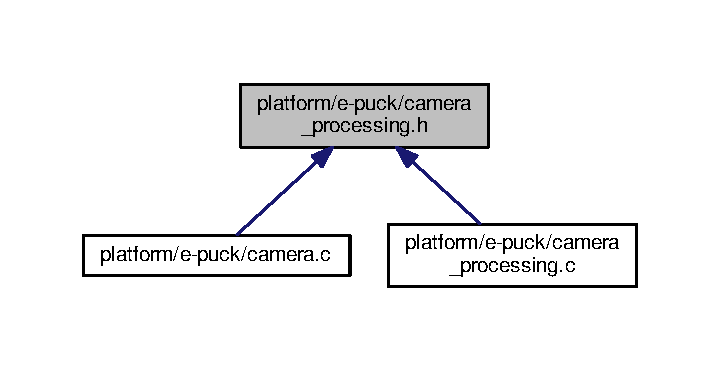
\includegraphics[width=346pt]{de/d9b/camera__processing_8h__dep__incl}
\end{center}
\end{figure}
\subsection*{Functions}
\begin{DoxyCompactItemize}
\item 
void \hyperlink{camera__processing_8h_a805427a51bfe2cf4d675d7cb479b819b}{convert\+R\+G\+B565\+To\+R\+G\+B888} (unsigned char rgb565\mbox{[}$\,$\mbox{]}, unsigned char rgb888\mbox{[}$\,$\mbox{]})
\item 
void \hyperlink{camera__processing_8h_afd2b8279decc2ab40000170b5506d385}{get\+R\+G\+B565at} (char $\ast$buffer, unsigned char rgb585\mbox{[}$\,$\mbox{]}, int x, int y)
\item 
void \hyperlink{camera__processing_8h_a8cfb72ecb08503eca4d6efc58b9987f2}{get\+R\+G\+B888at} (char $\ast$buffer, unsigned char rgb888\mbox{[}$\,$\mbox{]}, int x, int y)
\item 
char \hyperlink{camera__processing_8h_a8655b5660f79ef090db798451f1ed701}{nearest\+Neighbor\+R\+G\+B} (unsigned char $\ast$rbg888, char flag)
\item 
char \hyperlink{camera__processing_8h_ad921ae36e7f4fb378e1b67c2d1817244}{brushed\+Color\+From\+R\+G\+B565} (unsigned char rgb565\mbox{[}$\,$\mbox{]}, char flag)
\item 
char \hyperlink{camera__processing_8h_a587d4ed6a588eacad21baf2ac5aa1f10}{get\+Brushed\+Color\+At} (char $\ast$buffer, char flag, int x, int y, int w)
\end{DoxyCompactItemize}


\subsection{Detailed Description}
\begin{DoxyAuthor}{Author}
Yuri Kaszubowski Lopes \href{mailto:yurikazuba@gmail.com}{\tt yurikazuba@gmail.\+com} 
\end{DoxyAuthor}
\begin{DoxyVersion}{Version}
1.\+0
\end{DoxyVersion}
\begin{DoxyDate}{Date}
2014 
\end{DoxyDate}


\subsection{Function Documentation}
\hypertarget{camera__processing_8h_ad921ae36e7f4fb378e1b67c2d1817244}{}\index{camera\+\_\+processing.\+h@{camera\+\_\+processing.\+h}!brushed\+Color\+From\+R\+G\+B565@{brushed\+Color\+From\+R\+G\+B565}}
\index{brushed\+Color\+From\+R\+G\+B565@{brushed\+Color\+From\+R\+G\+B565}!camera\+\_\+processing.\+h@{camera\+\_\+processing.\+h}}
\subsubsection[{brushed\+Color\+From\+R\+G\+B565}]{\setlength{\rightskip}{0pt plus 5cm}char brushed\+Color\+From\+R\+G\+B565 (
\begin{DoxyParamCaption}
\item[{unsigned char}]{rgb565\mbox{[}$\,$\mbox{]}, }
\item[{char}]{flag}
\end{DoxyParamCaption}
)}\label{camera__processing_8h_ad921ae36e7f4fb378e1b67c2d1817244}


Definition at line 88 of file camera\+\_\+processing.\+c.

\hypertarget{camera__processing_8h_a805427a51bfe2cf4d675d7cb479b819b}{}\index{camera\+\_\+processing.\+h@{camera\+\_\+processing.\+h}!convert\+R\+G\+B565\+To\+R\+G\+B888@{convert\+R\+G\+B565\+To\+R\+G\+B888}}
\index{convert\+R\+G\+B565\+To\+R\+G\+B888@{convert\+R\+G\+B565\+To\+R\+G\+B888}!camera\+\_\+processing.\+h@{camera\+\_\+processing.\+h}}
\subsubsection[{convert\+R\+G\+B565\+To\+R\+G\+B888}]{\setlength{\rightskip}{0pt plus 5cm}void convert\+R\+G\+B565\+To\+R\+G\+B888 (
\begin{DoxyParamCaption}
\item[{unsigned char}]{rgb565\mbox{[}$\,$\mbox{]}, }
\item[{unsigned char}]{rgb888\mbox{[}$\,$\mbox{]}}
\end{DoxyParamCaption}
)}\label{camera__processing_8h_a805427a51bfe2cf4d675d7cb479b819b}


Definition at line 17 of file camera\+\_\+processing.\+c.

\hypertarget{camera__processing_8h_a587d4ed6a588eacad21baf2ac5aa1f10}{}\index{camera\+\_\+processing.\+h@{camera\+\_\+processing.\+h}!get\+Brushed\+Color\+At@{get\+Brushed\+Color\+At}}
\index{get\+Brushed\+Color\+At@{get\+Brushed\+Color\+At}!camera\+\_\+processing.\+h@{camera\+\_\+processing.\+h}}
\subsubsection[{get\+Brushed\+Color\+At}]{\setlength{\rightskip}{0pt plus 5cm}char get\+Brushed\+Color\+At (
\begin{DoxyParamCaption}
\item[{char $\ast$}]{buffer, }
\item[{char}]{flag, }
\item[{int}]{x, }
\item[{int}]{y, }
\item[{int}]{w}
\end{DoxyParamCaption}
)}\label{camera__processing_8h_a587d4ed6a588eacad21baf2ac5aa1f10}


Definition at line 111 of file camera\+\_\+processing.\+c.

\hypertarget{camera__processing_8h_afd2b8279decc2ab40000170b5506d385}{}\index{camera\+\_\+processing.\+h@{camera\+\_\+processing.\+h}!get\+R\+G\+B565at@{get\+R\+G\+B565at}}
\index{get\+R\+G\+B565at@{get\+R\+G\+B565at}!camera\+\_\+processing.\+h@{camera\+\_\+processing.\+h}}
\subsubsection[{get\+R\+G\+B565at}]{\setlength{\rightskip}{0pt plus 5cm}void get\+R\+G\+B565at (
\begin{DoxyParamCaption}
\item[{char $\ast$}]{buffer, }
\item[{unsigned char}]{rgb585\mbox{[}$\,$\mbox{]}, }
\item[{int}]{x, }
\item[{int}]{y}
\end{DoxyParamCaption}
)}\label{camera__processing_8h_afd2b8279decc2ab40000170b5506d385}


Definition at line 23 of file camera\+\_\+processing.\+c.

\hypertarget{camera__processing_8h_a8cfb72ecb08503eca4d6efc58b9987f2}{}\index{camera\+\_\+processing.\+h@{camera\+\_\+processing.\+h}!get\+R\+G\+B888at@{get\+R\+G\+B888at}}
\index{get\+R\+G\+B888at@{get\+R\+G\+B888at}!camera\+\_\+processing.\+h@{camera\+\_\+processing.\+h}}
\subsubsection[{get\+R\+G\+B888at}]{\setlength{\rightskip}{0pt plus 5cm}void get\+R\+G\+B888at (
\begin{DoxyParamCaption}
\item[{char $\ast$}]{buffer, }
\item[{unsigned char}]{rgb888\mbox{[}$\,$\mbox{]}, }
\item[{int}]{x, }
\item[{int}]{y}
\end{DoxyParamCaption}
)}\label{camera__processing_8h_a8cfb72ecb08503eca4d6efc58b9987f2}


Definition at line 28 of file camera\+\_\+processing.\+c.

\hypertarget{camera__processing_8h_a8655b5660f79ef090db798451f1ed701}{}\index{camera\+\_\+processing.\+h@{camera\+\_\+processing.\+h}!nearest\+Neighbor\+R\+G\+B@{nearest\+Neighbor\+R\+G\+B}}
\index{nearest\+Neighbor\+R\+G\+B@{nearest\+Neighbor\+R\+G\+B}!camera\+\_\+processing.\+h@{camera\+\_\+processing.\+h}}
\subsubsection[{nearest\+Neighbor\+R\+G\+B}]{\setlength{\rightskip}{0pt plus 5cm}char nearest\+Neighbor\+R\+G\+B (
\begin{DoxyParamCaption}
\item[{unsigned char $\ast$}]{rbg888, }
\item[{char}]{flag}
\end{DoxyParamCaption}
)}\label{camera__processing_8h_a8655b5660f79ef090db798451f1ed701}


Definition at line 52 of file camera\+\_\+processing.\+c.


\hypertarget{DSPIC30F6014A__HDI_8h}{}\section{platform/e-\/puck/\+D\+S\+P\+I\+C30\+F6014\+A\+\_\+\+H\+D\+I.h File Reference}
\label{DSPIC30F6014A__HDI_8h}\index{platform/e-\/puck/\+D\+S\+P\+I\+C30\+F6014\+A\+\_\+\+H\+D\+I.\+h@{platform/e-\/puck/\+D\+S\+P\+I\+C30\+F6014\+A\+\_\+\+H\+D\+I.\+h}}


declares e-\/puck specific types and preprocessor variables  


{\ttfamily \#include \char`\"{}library/motor\+\_\+led/e\+\_\+epuck\+\_\+ports.\+h\char`\"{}}\\*
Include dependency graph for D\+S\+P\+I\+C30\+F6014\+A\+\_\+\+H\+D\+I.\+h\+:\nopagebreak
\begin{figure}[H]
\begin{center}
\leavevmode
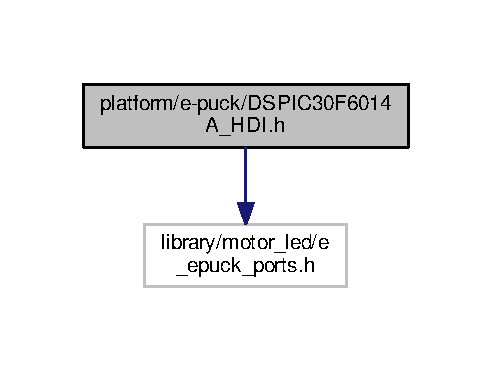
\includegraphics[width=236pt]{d3/d86/DSPIC30F6014A__HDI_8h__incl}
\end{center}
\end{figure}
This graph shows which files directly or indirectly include this file\+:
\nopagebreak
\begin{figure}[H]
\begin{center}
\leavevmode
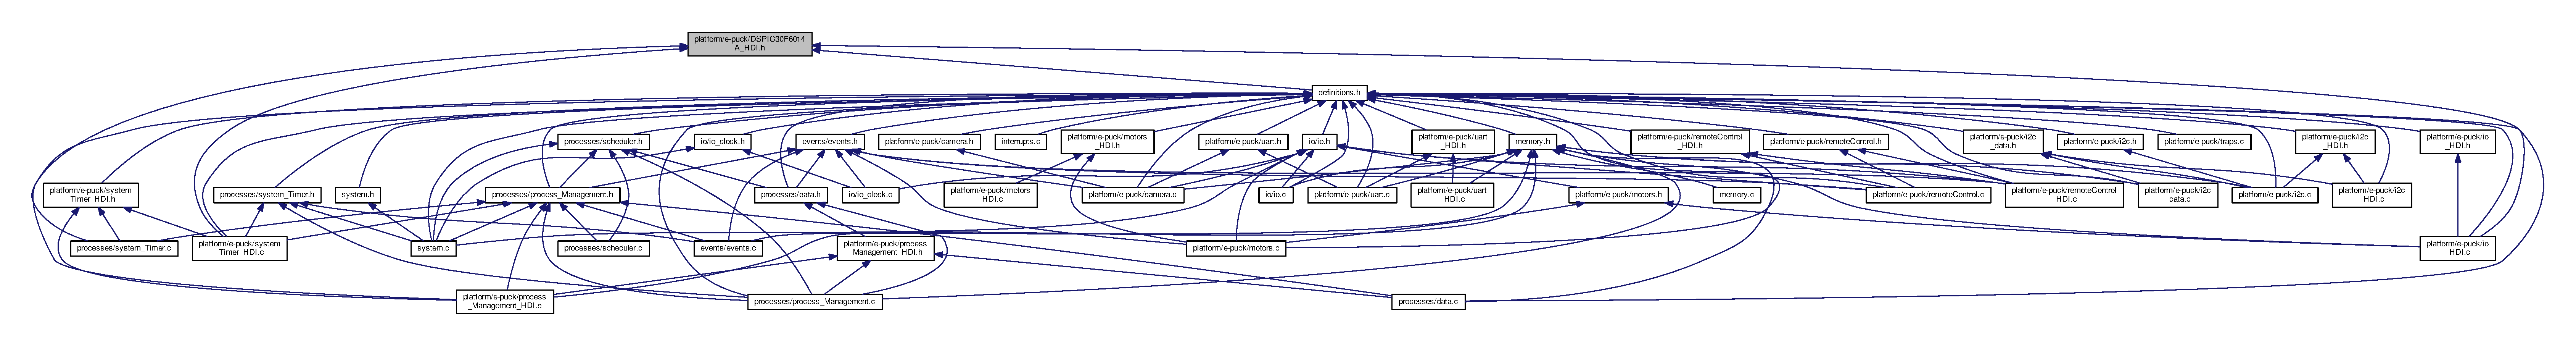
\includegraphics[width=350pt]{db/d10/DSPIC30F6014A__HDI_8h__dep__incl}
\end{center}
\end{figure}
\subsection*{Macros}
\begin{DoxyCompactItemize}
\item 
\#define \hyperlink{DSPIC30F6014A__HDI_8h_a7702c960dffab411cc9b8ff73050f80d}{A\+D\+D\+R\+E\+S\+S\+\_\+\+I\+V\+T}~0x000004
\item 
\#define \hyperlink{DSPIC30F6014A__HDI_8h_a9cc033666041c0dcb074a39c4c3fb71f}{A\+D\+D\+R\+E\+S\+S\+\_\+\+I\+T\+V\+\_\+\+O\+S\+C\+\_\+\+F\+A\+I\+L}~\hyperlink{DSPIC30F6014A__HDI_8h_a7702c960dffab411cc9b8ff73050f80d}{A\+D\+D\+R\+E\+S\+S\+\_\+\+I\+V\+T}+2
\item 
\#define \hyperlink{DSPIC30F6014A__HDI_8h_a580df2d89a9bd567c0961ae9ec6fce8f}{A\+D\+D\+R\+E\+S\+S\+\_\+\+I\+T\+V\+\_\+\+A\+D\+D\+R\+E\+S\+S\+\_\+\+E\+R\+R\+O\+R}~\hyperlink{DSPIC30F6014A__HDI_8h_a7702c960dffab411cc9b8ff73050f80d}{A\+D\+D\+R\+E\+S\+S\+\_\+\+I\+V\+T}+4
\item 
\#define \hyperlink{DSPIC30F6014A__HDI_8h_abbaa1320b64c9aab11e49dcaebfb6a9a}{A\+D\+D\+R\+E\+S\+S\+\_\+\+I\+T\+V\+\_\+\+S\+T\+A\+C\+K\+\_\+\+E\+R\+R\+O\+R}~\hyperlink{DSPIC30F6014A__HDI_8h_a7702c960dffab411cc9b8ff73050f80d}{A\+D\+D\+R\+E\+S\+S\+\_\+\+I\+V\+T}+6
\item 
\#define \hyperlink{DSPIC30F6014A__HDI_8h_a0431d3a5ce33898fcd5eb343101eca65}{A\+D\+D\+R\+E\+S\+S\+\_\+\+I\+T\+V\+\_\+\+M\+A\+T\+H\+\_\+\+E\+R\+R\+O\+R}~\hyperlink{DSPIC30F6014A__HDI_8h_a7702c960dffab411cc9b8ff73050f80d}{A\+D\+D\+R\+E\+S\+S\+\_\+\+I\+V\+T}+8
\item 
\#define \hyperlink{DSPIC30F6014A__HDI_8h_a7d47228ffb61ec3118d613034c8fa560}{A\+D\+D\+R\+E\+S\+S\+\_\+\+I\+V\+T\+\_\+\+T1}~0x00001\+A
\item 
\#define \hyperlink{DSPIC30F6014A__HDI_8h_ae3c44069639816f295543638b367b89a}{A\+D\+D\+R\+E\+S\+S\+\_\+\+A\+I\+V\+T}~0x000084
\item 
\#define \hyperlink{DSPIC30F6014A__HDI_8h_a35e587ecff2c88b0b152da2780350c67}{A\+D\+D\+R\+E\+S\+S\+\_\+\+A\+I\+T\+V\+\_\+\+O\+S\+C\+\_\+\+F\+A\+I\+L}~\hyperlink{DSPIC30F6014A__HDI_8h_ae3c44069639816f295543638b367b89a}{A\+D\+D\+R\+E\+S\+S\+\_\+\+A\+I\+V\+T}+2
\item 
\#define \hyperlink{DSPIC30F6014A__HDI_8h_a3cc13527af6ad1f3b69348add12febad}{A\+D\+D\+R\+E\+S\+S\+\_\+\+A\+I\+T\+V\+\_\+\+A\+D\+D\+R\+E\+S\+S\+\_\+\+E\+R\+R\+O\+R}~\hyperlink{DSPIC30F6014A__HDI_8h_ae3c44069639816f295543638b367b89a}{A\+D\+D\+R\+E\+S\+S\+\_\+\+A\+I\+V\+T}+4
\item 
\#define \hyperlink{DSPIC30F6014A__HDI_8h_a7ee4d9f555fe279b9ff12c929c912236}{A\+D\+D\+R\+E\+S\+S\+\_\+\+A\+I\+T\+V\+\_\+\+S\+T\+A\+C\+K\+\_\+\+E\+R\+R\+O\+R}~\hyperlink{DSPIC30F6014A__HDI_8h_ae3c44069639816f295543638b367b89a}{A\+D\+D\+R\+E\+S\+S\+\_\+\+A\+I\+V\+T}+6
\item 
\#define \hyperlink{DSPIC30F6014A__HDI_8h_a38ba5f4837f45684c018c28eb245cb9d}{A\+D\+D\+R\+E\+S\+S\+\_\+\+A\+I\+T\+V\+\_\+\+M\+A\+T\+H\+\_\+\+E\+R\+R\+O\+R}~\hyperlink{DSPIC30F6014A__HDI_8h_ae3c44069639816f295543638b367b89a}{A\+D\+D\+R\+E\+S\+S\+\_\+\+A\+I\+V\+T}+8
\item 
\#define \hyperlink{DSPIC30F6014A__HDI_8h_a5c8bbde3591fc148b1c88f24b1b4b5a5}{A\+D\+D\+R\+E\+S\+S\+\_\+\+A\+I\+V\+T\+\_\+\+T1}~0x00009\+A
\end{DoxyCompactItemize}


\subsection{Detailed Description}
declares e-\/puck specific types and preprocessor variables 

\begin{DoxyAuthor}{Author}
Stefan M. Trenkwalder \href{mailto:s.trenkwalder@openswarm.org}{\tt s.\+trenkwalder@openswarm.\+org}
\end{DoxyAuthor}
\begin{DoxyVersion}{Version}
1.\+0
\end{DoxyVersion}
\begin{DoxyDate}{Date}
07 July 2014
\end{DoxyDate}
\begin{DoxyCopyright}{Copyright}
adapted Free\+B\+S\+D License (see \href{http://openswarm.org/license}{\tt http\+://openswarm.\+org/license}) 
\end{DoxyCopyright}


\subsection{Macro Definition Documentation}
\hypertarget{DSPIC30F6014A__HDI_8h_a3cc13527af6ad1f3b69348add12febad}{}\index{D\+S\+P\+I\+C30\+F6014\+A\+\_\+\+H\+D\+I.\+h@{D\+S\+P\+I\+C30\+F6014\+A\+\_\+\+H\+D\+I.\+h}!A\+D\+D\+R\+E\+S\+S\+\_\+\+A\+I\+T\+V\+\_\+\+A\+D\+D\+R\+E\+S\+S\+\_\+\+E\+R\+R\+O\+R@{A\+D\+D\+R\+E\+S\+S\+\_\+\+A\+I\+T\+V\+\_\+\+A\+D\+D\+R\+E\+S\+S\+\_\+\+E\+R\+R\+O\+R}}
\index{A\+D\+D\+R\+E\+S\+S\+\_\+\+A\+I\+T\+V\+\_\+\+A\+D\+D\+R\+E\+S\+S\+\_\+\+E\+R\+R\+O\+R@{A\+D\+D\+R\+E\+S\+S\+\_\+\+A\+I\+T\+V\+\_\+\+A\+D\+D\+R\+E\+S\+S\+\_\+\+E\+R\+R\+O\+R}!D\+S\+P\+I\+C30\+F6014\+A\+\_\+\+H\+D\+I.\+h@{D\+S\+P\+I\+C30\+F6014\+A\+\_\+\+H\+D\+I.\+h}}
\subsubsection[{A\+D\+D\+R\+E\+S\+S\+\_\+\+A\+I\+T\+V\+\_\+\+A\+D\+D\+R\+E\+S\+S\+\_\+\+E\+R\+R\+O\+R}]{\setlength{\rightskip}{0pt plus 5cm}\#define A\+D\+D\+R\+E\+S\+S\+\_\+\+A\+I\+T\+V\+\_\+\+A\+D\+D\+R\+E\+S\+S\+\_\+\+E\+R\+R\+O\+R~{\bf A\+D\+D\+R\+E\+S\+S\+\_\+\+A\+I\+V\+T}+4}\label{DSPIC30F6014A__HDI_8h_a3cc13527af6ad1f3b69348add12febad}


Definition at line 74 of file D\+S\+P\+I\+C30\+F6014\+A\+\_\+\+H\+D\+I.\+h.

\hypertarget{DSPIC30F6014A__HDI_8h_a38ba5f4837f45684c018c28eb245cb9d}{}\index{D\+S\+P\+I\+C30\+F6014\+A\+\_\+\+H\+D\+I.\+h@{D\+S\+P\+I\+C30\+F6014\+A\+\_\+\+H\+D\+I.\+h}!A\+D\+D\+R\+E\+S\+S\+\_\+\+A\+I\+T\+V\+\_\+\+M\+A\+T\+H\+\_\+\+E\+R\+R\+O\+R@{A\+D\+D\+R\+E\+S\+S\+\_\+\+A\+I\+T\+V\+\_\+\+M\+A\+T\+H\+\_\+\+E\+R\+R\+O\+R}}
\index{A\+D\+D\+R\+E\+S\+S\+\_\+\+A\+I\+T\+V\+\_\+\+M\+A\+T\+H\+\_\+\+E\+R\+R\+O\+R@{A\+D\+D\+R\+E\+S\+S\+\_\+\+A\+I\+T\+V\+\_\+\+M\+A\+T\+H\+\_\+\+E\+R\+R\+O\+R}!D\+S\+P\+I\+C30\+F6014\+A\+\_\+\+H\+D\+I.\+h@{D\+S\+P\+I\+C30\+F6014\+A\+\_\+\+H\+D\+I.\+h}}
\subsubsection[{A\+D\+D\+R\+E\+S\+S\+\_\+\+A\+I\+T\+V\+\_\+\+M\+A\+T\+H\+\_\+\+E\+R\+R\+O\+R}]{\setlength{\rightskip}{0pt plus 5cm}\#define A\+D\+D\+R\+E\+S\+S\+\_\+\+A\+I\+T\+V\+\_\+\+M\+A\+T\+H\+\_\+\+E\+R\+R\+O\+R~{\bf A\+D\+D\+R\+E\+S\+S\+\_\+\+A\+I\+V\+T}+8}\label{DSPIC30F6014A__HDI_8h_a38ba5f4837f45684c018c28eb245cb9d}


Definition at line 76 of file D\+S\+P\+I\+C30\+F6014\+A\+\_\+\+H\+D\+I.\+h.

\hypertarget{DSPIC30F6014A__HDI_8h_a35e587ecff2c88b0b152da2780350c67}{}\index{D\+S\+P\+I\+C30\+F6014\+A\+\_\+\+H\+D\+I.\+h@{D\+S\+P\+I\+C30\+F6014\+A\+\_\+\+H\+D\+I.\+h}!A\+D\+D\+R\+E\+S\+S\+\_\+\+A\+I\+T\+V\+\_\+\+O\+S\+C\+\_\+\+F\+A\+I\+L@{A\+D\+D\+R\+E\+S\+S\+\_\+\+A\+I\+T\+V\+\_\+\+O\+S\+C\+\_\+\+F\+A\+I\+L}}
\index{A\+D\+D\+R\+E\+S\+S\+\_\+\+A\+I\+T\+V\+\_\+\+O\+S\+C\+\_\+\+F\+A\+I\+L@{A\+D\+D\+R\+E\+S\+S\+\_\+\+A\+I\+T\+V\+\_\+\+O\+S\+C\+\_\+\+F\+A\+I\+L}!D\+S\+P\+I\+C30\+F6014\+A\+\_\+\+H\+D\+I.\+h@{D\+S\+P\+I\+C30\+F6014\+A\+\_\+\+H\+D\+I.\+h}}
\subsubsection[{A\+D\+D\+R\+E\+S\+S\+\_\+\+A\+I\+T\+V\+\_\+\+O\+S\+C\+\_\+\+F\+A\+I\+L}]{\setlength{\rightskip}{0pt plus 5cm}\#define A\+D\+D\+R\+E\+S\+S\+\_\+\+A\+I\+T\+V\+\_\+\+O\+S\+C\+\_\+\+F\+A\+I\+L~{\bf A\+D\+D\+R\+E\+S\+S\+\_\+\+A\+I\+V\+T}+2}\label{DSPIC30F6014A__HDI_8h_a35e587ecff2c88b0b152da2780350c67}


Definition at line 73 of file D\+S\+P\+I\+C30\+F6014\+A\+\_\+\+H\+D\+I.\+h.

\hypertarget{DSPIC30F6014A__HDI_8h_a7ee4d9f555fe279b9ff12c929c912236}{}\index{D\+S\+P\+I\+C30\+F6014\+A\+\_\+\+H\+D\+I.\+h@{D\+S\+P\+I\+C30\+F6014\+A\+\_\+\+H\+D\+I.\+h}!A\+D\+D\+R\+E\+S\+S\+\_\+\+A\+I\+T\+V\+\_\+\+S\+T\+A\+C\+K\+\_\+\+E\+R\+R\+O\+R@{A\+D\+D\+R\+E\+S\+S\+\_\+\+A\+I\+T\+V\+\_\+\+S\+T\+A\+C\+K\+\_\+\+E\+R\+R\+O\+R}}
\index{A\+D\+D\+R\+E\+S\+S\+\_\+\+A\+I\+T\+V\+\_\+\+S\+T\+A\+C\+K\+\_\+\+E\+R\+R\+O\+R@{A\+D\+D\+R\+E\+S\+S\+\_\+\+A\+I\+T\+V\+\_\+\+S\+T\+A\+C\+K\+\_\+\+E\+R\+R\+O\+R}!D\+S\+P\+I\+C30\+F6014\+A\+\_\+\+H\+D\+I.\+h@{D\+S\+P\+I\+C30\+F6014\+A\+\_\+\+H\+D\+I.\+h}}
\subsubsection[{A\+D\+D\+R\+E\+S\+S\+\_\+\+A\+I\+T\+V\+\_\+\+S\+T\+A\+C\+K\+\_\+\+E\+R\+R\+O\+R}]{\setlength{\rightskip}{0pt plus 5cm}\#define A\+D\+D\+R\+E\+S\+S\+\_\+\+A\+I\+T\+V\+\_\+\+S\+T\+A\+C\+K\+\_\+\+E\+R\+R\+O\+R~{\bf A\+D\+D\+R\+E\+S\+S\+\_\+\+A\+I\+V\+T}+6}\label{DSPIC30F6014A__HDI_8h_a7ee4d9f555fe279b9ff12c929c912236}


Definition at line 75 of file D\+S\+P\+I\+C30\+F6014\+A\+\_\+\+H\+D\+I.\+h.

\hypertarget{DSPIC30F6014A__HDI_8h_ae3c44069639816f295543638b367b89a}{}\index{D\+S\+P\+I\+C30\+F6014\+A\+\_\+\+H\+D\+I.\+h@{D\+S\+P\+I\+C30\+F6014\+A\+\_\+\+H\+D\+I.\+h}!A\+D\+D\+R\+E\+S\+S\+\_\+\+A\+I\+V\+T@{A\+D\+D\+R\+E\+S\+S\+\_\+\+A\+I\+V\+T}}
\index{A\+D\+D\+R\+E\+S\+S\+\_\+\+A\+I\+V\+T@{A\+D\+D\+R\+E\+S\+S\+\_\+\+A\+I\+V\+T}!D\+S\+P\+I\+C30\+F6014\+A\+\_\+\+H\+D\+I.\+h@{D\+S\+P\+I\+C30\+F6014\+A\+\_\+\+H\+D\+I.\+h}}
\subsubsection[{A\+D\+D\+R\+E\+S\+S\+\_\+\+A\+I\+V\+T}]{\setlength{\rightskip}{0pt plus 5cm}\#define A\+D\+D\+R\+E\+S\+S\+\_\+\+A\+I\+V\+T~0x000084}\label{DSPIC30F6014A__HDI_8h_ae3c44069639816f295543638b367b89a}


Definition at line 72 of file D\+S\+P\+I\+C30\+F6014\+A\+\_\+\+H\+D\+I.\+h.

\hypertarget{DSPIC30F6014A__HDI_8h_a5c8bbde3591fc148b1c88f24b1b4b5a5}{}\index{D\+S\+P\+I\+C30\+F6014\+A\+\_\+\+H\+D\+I.\+h@{D\+S\+P\+I\+C30\+F6014\+A\+\_\+\+H\+D\+I.\+h}!A\+D\+D\+R\+E\+S\+S\+\_\+\+A\+I\+V\+T\+\_\+\+T1@{A\+D\+D\+R\+E\+S\+S\+\_\+\+A\+I\+V\+T\+\_\+\+T1}}
\index{A\+D\+D\+R\+E\+S\+S\+\_\+\+A\+I\+V\+T\+\_\+\+T1@{A\+D\+D\+R\+E\+S\+S\+\_\+\+A\+I\+V\+T\+\_\+\+T1}!D\+S\+P\+I\+C30\+F6014\+A\+\_\+\+H\+D\+I.\+h@{D\+S\+P\+I\+C30\+F6014\+A\+\_\+\+H\+D\+I.\+h}}
\subsubsection[{A\+D\+D\+R\+E\+S\+S\+\_\+\+A\+I\+V\+T\+\_\+\+T1}]{\setlength{\rightskip}{0pt plus 5cm}\#define A\+D\+D\+R\+E\+S\+S\+\_\+\+A\+I\+V\+T\+\_\+\+T1~0x00009\+A}\label{DSPIC30F6014A__HDI_8h_a5c8bbde3591fc148b1c88f24b1b4b5a5}


Definition at line 77 of file D\+S\+P\+I\+C30\+F6014\+A\+\_\+\+H\+D\+I.\+h.

\hypertarget{DSPIC30F6014A__HDI_8h_a580df2d89a9bd567c0961ae9ec6fce8f}{}\index{D\+S\+P\+I\+C30\+F6014\+A\+\_\+\+H\+D\+I.\+h@{D\+S\+P\+I\+C30\+F6014\+A\+\_\+\+H\+D\+I.\+h}!A\+D\+D\+R\+E\+S\+S\+\_\+\+I\+T\+V\+\_\+\+A\+D\+D\+R\+E\+S\+S\+\_\+\+E\+R\+R\+O\+R@{A\+D\+D\+R\+E\+S\+S\+\_\+\+I\+T\+V\+\_\+\+A\+D\+D\+R\+E\+S\+S\+\_\+\+E\+R\+R\+O\+R}}
\index{A\+D\+D\+R\+E\+S\+S\+\_\+\+I\+T\+V\+\_\+\+A\+D\+D\+R\+E\+S\+S\+\_\+\+E\+R\+R\+O\+R@{A\+D\+D\+R\+E\+S\+S\+\_\+\+I\+T\+V\+\_\+\+A\+D\+D\+R\+E\+S\+S\+\_\+\+E\+R\+R\+O\+R}!D\+S\+P\+I\+C30\+F6014\+A\+\_\+\+H\+D\+I.\+h@{D\+S\+P\+I\+C30\+F6014\+A\+\_\+\+H\+D\+I.\+h}}
\subsubsection[{A\+D\+D\+R\+E\+S\+S\+\_\+\+I\+T\+V\+\_\+\+A\+D\+D\+R\+E\+S\+S\+\_\+\+E\+R\+R\+O\+R}]{\setlength{\rightskip}{0pt plus 5cm}\#define A\+D\+D\+R\+E\+S\+S\+\_\+\+I\+T\+V\+\_\+\+A\+D\+D\+R\+E\+S\+S\+\_\+\+E\+R\+R\+O\+R~{\bf A\+D\+D\+R\+E\+S\+S\+\_\+\+I\+V\+T}+4}\label{DSPIC30F6014A__HDI_8h_a580df2d89a9bd567c0961ae9ec6fce8f}


Definition at line 66 of file D\+S\+P\+I\+C30\+F6014\+A\+\_\+\+H\+D\+I.\+h.

\hypertarget{DSPIC30F6014A__HDI_8h_a0431d3a5ce33898fcd5eb343101eca65}{}\index{D\+S\+P\+I\+C30\+F6014\+A\+\_\+\+H\+D\+I.\+h@{D\+S\+P\+I\+C30\+F6014\+A\+\_\+\+H\+D\+I.\+h}!A\+D\+D\+R\+E\+S\+S\+\_\+\+I\+T\+V\+\_\+\+M\+A\+T\+H\+\_\+\+E\+R\+R\+O\+R@{A\+D\+D\+R\+E\+S\+S\+\_\+\+I\+T\+V\+\_\+\+M\+A\+T\+H\+\_\+\+E\+R\+R\+O\+R}}
\index{A\+D\+D\+R\+E\+S\+S\+\_\+\+I\+T\+V\+\_\+\+M\+A\+T\+H\+\_\+\+E\+R\+R\+O\+R@{A\+D\+D\+R\+E\+S\+S\+\_\+\+I\+T\+V\+\_\+\+M\+A\+T\+H\+\_\+\+E\+R\+R\+O\+R}!D\+S\+P\+I\+C30\+F6014\+A\+\_\+\+H\+D\+I.\+h@{D\+S\+P\+I\+C30\+F6014\+A\+\_\+\+H\+D\+I.\+h}}
\subsubsection[{A\+D\+D\+R\+E\+S\+S\+\_\+\+I\+T\+V\+\_\+\+M\+A\+T\+H\+\_\+\+E\+R\+R\+O\+R}]{\setlength{\rightskip}{0pt plus 5cm}\#define A\+D\+D\+R\+E\+S\+S\+\_\+\+I\+T\+V\+\_\+\+M\+A\+T\+H\+\_\+\+E\+R\+R\+O\+R~{\bf A\+D\+D\+R\+E\+S\+S\+\_\+\+I\+V\+T}+8}\label{DSPIC30F6014A__HDI_8h_a0431d3a5ce33898fcd5eb343101eca65}


Definition at line 68 of file D\+S\+P\+I\+C30\+F6014\+A\+\_\+\+H\+D\+I.\+h.

\hypertarget{DSPIC30F6014A__HDI_8h_a9cc033666041c0dcb074a39c4c3fb71f}{}\index{D\+S\+P\+I\+C30\+F6014\+A\+\_\+\+H\+D\+I.\+h@{D\+S\+P\+I\+C30\+F6014\+A\+\_\+\+H\+D\+I.\+h}!A\+D\+D\+R\+E\+S\+S\+\_\+\+I\+T\+V\+\_\+\+O\+S\+C\+\_\+\+F\+A\+I\+L@{A\+D\+D\+R\+E\+S\+S\+\_\+\+I\+T\+V\+\_\+\+O\+S\+C\+\_\+\+F\+A\+I\+L}}
\index{A\+D\+D\+R\+E\+S\+S\+\_\+\+I\+T\+V\+\_\+\+O\+S\+C\+\_\+\+F\+A\+I\+L@{A\+D\+D\+R\+E\+S\+S\+\_\+\+I\+T\+V\+\_\+\+O\+S\+C\+\_\+\+F\+A\+I\+L}!D\+S\+P\+I\+C30\+F6014\+A\+\_\+\+H\+D\+I.\+h@{D\+S\+P\+I\+C30\+F6014\+A\+\_\+\+H\+D\+I.\+h}}
\subsubsection[{A\+D\+D\+R\+E\+S\+S\+\_\+\+I\+T\+V\+\_\+\+O\+S\+C\+\_\+\+F\+A\+I\+L}]{\setlength{\rightskip}{0pt plus 5cm}\#define A\+D\+D\+R\+E\+S\+S\+\_\+\+I\+T\+V\+\_\+\+O\+S\+C\+\_\+\+F\+A\+I\+L~{\bf A\+D\+D\+R\+E\+S\+S\+\_\+\+I\+V\+T}+2}\label{DSPIC30F6014A__HDI_8h_a9cc033666041c0dcb074a39c4c3fb71f}


Definition at line 65 of file D\+S\+P\+I\+C30\+F6014\+A\+\_\+\+H\+D\+I.\+h.

\hypertarget{DSPIC30F6014A__HDI_8h_abbaa1320b64c9aab11e49dcaebfb6a9a}{}\index{D\+S\+P\+I\+C30\+F6014\+A\+\_\+\+H\+D\+I.\+h@{D\+S\+P\+I\+C30\+F6014\+A\+\_\+\+H\+D\+I.\+h}!A\+D\+D\+R\+E\+S\+S\+\_\+\+I\+T\+V\+\_\+\+S\+T\+A\+C\+K\+\_\+\+E\+R\+R\+O\+R@{A\+D\+D\+R\+E\+S\+S\+\_\+\+I\+T\+V\+\_\+\+S\+T\+A\+C\+K\+\_\+\+E\+R\+R\+O\+R}}
\index{A\+D\+D\+R\+E\+S\+S\+\_\+\+I\+T\+V\+\_\+\+S\+T\+A\+C\+K\+\_\+\+E\+R\+R\+O\+R@{A\+D\+D\+R\+E\+S\+S\+\_\+\+I\+T\+V\+\_\+\+S\+T\+A\+C\+K\+\_\+\+E\+R\+R\+O\+R}!D\+S\+P\+I\+C30\+F6014\+A\+\_\+\+H\+D\+I.\+h@{D\+S\+P\+I\+C30\+F6014\+A\+\_\+\+H\+D\+I.\+h}}
\subsubsection[{A\+D\+D\+R\+E\+S\+S\+\_\+\+I\+T\+V\+\_\+\+S\+T\+A\+C\+K\+\_\+\+E\+R\+R\+O\+R}]{\setlength{\rightskip}{0pt plus 5cm}\#define A\+D\+D\+R\+E\+S\+S\+\_\+\+I\+T\+V\+\_\+\+S\+T\+A\+C\+K\+\_\+\+E\+R\+R\+O\+R~{\bf A\+D\+D\+R\+E\+S\+S\+\_\+\+I\+V\+T}+6}\label{DSPIC30F6014A__HDI_8h_abbaa1320b64c9aab11e49dcaebfb6a9a}


Definition at line 67 of file D\+S\+P\+I\+C30\+F6014\+A\+\_\+\+H\+D\+I.\+h.

\hypertarget{DSPIC30F6014A__HDI_8h_a7702c960dffab411cc9b8ff73050f80d}{}\index{D\+S\+P\+I\+C30\+F6014\+A\+\_\+\+H\+D\+I.\+h@{D\+S\+P\+I\+C30\+F6014\+A\+\_\+\+H\+D\+I.\+h}!A\+D\+D\+R\+E\+S\+S\+\_\+\+I\+V\+T@{A\+D\+D\+R\+E\+S\+S\+\_\+\+I\+V\+T}}
\index{A\+D\+D\+R\+E\+S\+S\+\_\+\+I\+V\+T@{A\+D\+D\+R\+E\+S\+S\+\_\+\+I\+V\+T}!D\+S\+P\+I\+C30\+F6014\+A\+\_\+\+H\+D\+I.\+h@{D\+S\+P\+I\+C30\+F6014\+A\+\_\+\+H\+D\+I.\+h}}
\subsubsection[{A\+D\+D\+R\+E\+S\+S\+\_\+\+I\+V\+T}]{\setlength{\rightskip}{0pt plus 5cm}\#define A\+D\+D\+R\+E\+S\+S\+\_\+\+I\+V\+T~0x000004}\label{DSPIC30F6014A__HDI_8h_a7702c960dffab411cc9b8ff73050f80d}


Definition at line 64 of file D\+S\+P\+I\+C30\+F6014\+A\+\_\+\+H\+D\+I.\+h.

\hypertarget{DSPIC30F6014A__HDI_8h_a7d47228ffb61ec3118d613034c8fa560}{}\index{D\+S\+P\+I\+C30\+F6014\+A\+\_\+\+H\+D\+I.\+h@{D\+S\+P\+I\+C30\+F6014\+A\+\_\+\+H\+D\+I.\+h}!A\+D\+D\+R\+E\+S\+S\+\_\+\+I\+V\+T\+\_\+\+T1@{A\+D\+D\+R\+E\+S\+S\+\_\+\+I\+V\+T\+\_\+\+T1}}
\index{A\+D\+D\+R\+E\+S\+S\+\_\+\+I\+V\+T\+\_\+\+T1@{A\+D\+D\+R\+E\+S\+S\+\_\+\+I\+V\+T\+\_\+\+T1}!D\+S\+P\+I\+C30\+F6014\+A\+\_\+\+H\+D\+I.\+h@{D\+S\+P\+I\+C30\+F6014\+A\+\_\+\+H\+D\+I.\+h}}
\subsubsection[{A\+D\+D\+R\+E\+S\+S\+\_\+\+I\+V\+T\+\_\+\+T1}]{\setlength{\rightskip}{0pt plus 5cm}\#define A\+D\+D\+R\+E\+S\+S\+\_\+\+I\+V\+T\+\_\+\+T1~0x00001\+A}\label{DSPIC30F6014A__HDI_8h_a7d47228ffb61ec3118d613034c8fa560}


Definition at line 69 of file D\+S\+P\+I\+C30\+F6014\+A\+\_\+\+H\+D\+I.\+h.


\hypertarget{i2c_8c}{}\section{platform/e-\/puck/i2c.c File Reference}
\label{i2c_8c}\index{platform/e-\/puck/i2c.\+c@{platform/e-\/puck/i2c.\+c}}


defines functions to read and write on the I2\+C interface.  


{\ttfamily \#include \char`\"{}i2c.\+h\char`\"{}}\\*
{\ttfamily \#include \char`\"{}i2c\+\_\+data.\+h\char`\"{}}\\*
{\ttfamily \#include \char`\"{}i2c\+\_\+\+H\+D\+I.\+h\char`\"{}}\\*
{\ttfamily \#include $<$stdlib.\+h$>$}\\*
{\ttfamily \#include $<$stdbool.\+h$>$}\\*
{\ttfamily \#include \char`\"{}../../definitions.\+h\char`\"{}}\\*
{\ttfamily \#include \char`\"{}../../memory.\+h\char`\"{}}\\*
{\ttfamily \#include \char`\"{}../../interrupts.\+h\char`\"{}}\\*
Include dependency graph for i2c.\+c\+:
\nopagebreak
\begin{figure}[H]
\begin{center}
\leavevmode
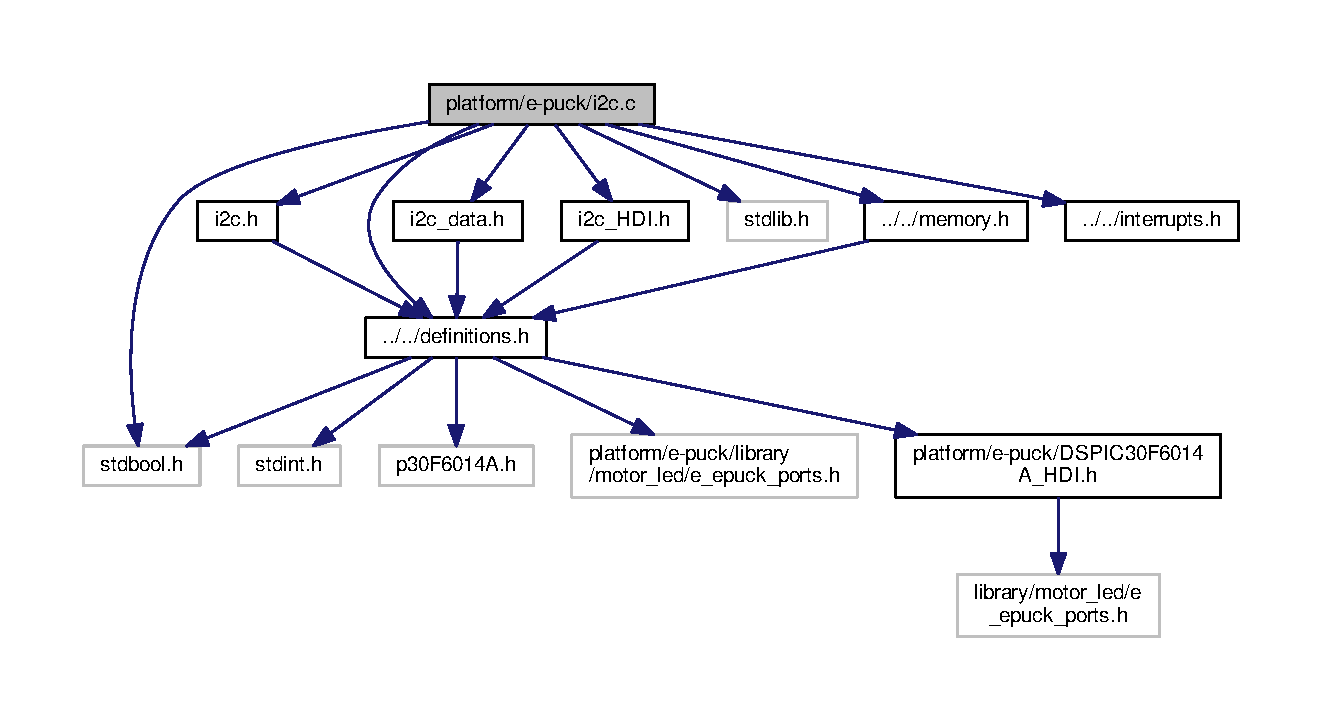
\includegraphics[width=350pt]{d6/d4e/i2c_8c__incl}
\end{center}
\end{figure}
\subsection*{Functions}
\begin{DoxyCompactItemize}
\item 
void \hyperlink{i2c_8c_a5760a8fc225d2d72f913c2b9cead750c}{Sys\+\_\+\+I2\+C\+\_\+\+Send\+\_\+\+Start} ()
\item 
void \hyperlink{i2c_8c_aea59a4077a8d5bd8657687837e3f0608}{Sys\+\_\+\+I2\+C\+\_\+\+Send\+\_\+\+Restart} (void)
\item 
void \hyperlink{i2c_8c_a7743095d9bff8142c1ad71f9373ccced}{Sys\+\_\+\+I2\+C\+\_\+\+Send\+\_\+\+Stop} (void)
\item 
void \hyperlink{i2c_8c_a884513154bff3409711c1e503c87c284}{Sys\+\_\+\+I2\+C\+\_\+\+Send\+\_\+\+A\+C\+K} (void)
\item 
void \hyperlink{i2c_8c_a3e04179756a1c2b23305eb861150ef27}{Sys\+\_\+\+I2\+C\+\_\+\+Send\+\_\+\+N\+A\+C\+K} (void)
\item 
void \hyperlink{i2c_8c_a5c9b97ea97adad15dcd2449471b3f99a}{Sys\+\_\+\+I2\+C\+\_\+\+Start\+\_\+\+Reading} (void)
\item 
char \hyperlink{i2c_8c_a1aa92e9c723a538dcf648f8613a1a1d3}{Sys\+\_\+\+I2\+C\+\_\+\+Read\+Byte} (void)
\item 
void \hyperlink{i2c_8c_a57b36c09636bc51eb2889106b972fe4d}{Sys\+\_\+\+I2\+C\+\_\+\+Write\+Byte} (\hyperlink{definitions_8h_adde6aaee8457bee49c2a92621fe22b79}{uint8} byte)
\item 
void \hyperlink{i2c_8c_a446fc07616c9db4f72b2331f8c7f4155}{Sys\+\_\+\+Init\+\_\+\+I2\+C} ()
\item 
void \hyperlink{i2c_8c_aeb4bfa683641abfe5fccbd24587b4259}{Sys\+\_\+\+Start\+\_\+\+I2\+C} ()
\item 
void \hyperlink{i2c_8c_ac0176dd64d977bfc72505f88d9ae608c}{Sys\+\_\+\+Pause\+\_\+\+I2\+C} ()
\item 
void \hyperlink{i2c_8c_a998450ded80998fc75f16fbcf8a30c43}{Sys\+\_\+\+Contine\+\_\+\+I2\+C} ()
\item 
void \hyperlink{i2c_8c_adc41d72cf5f017a96d06736c289ec578}{Sys\+\_\+\+Stop\+\_\+\+I2\+C} ()
\item 
void \hyperlink{i2c_8c_ad333b7abeb87e8f8c18d3dedd031ad5c}{Sys\+\_\+\+I2\+C\+\_\+\+Sent\+Bytes} (\hyperlink{definitions_8h_adde6aaee8457bee49c2a92621fe22b79}{uint8} address, \hyperlink{definitions_8h_adde6aaee8457bee49c2a92621fe22b79}{uint8} $\ast$bytes, \hyperlink{definitions_8h_a05f6b0ae8f6a6e135b0e290c25fe0e4e}{uint16} length)
\item 
void \hyperlink{i2c_8c_ab85476756c65b454eea96255916e22f9}{Sys\+\_\+\+I2\+C\+\_\+\+Read} (\hyperlink{definitions_8h_adde6aaee8457bee49c2a92621fe22b79}{uint8} address, \hyperlink{definitions_8h_adde6aaee8457bee49c2a92621fe22b79}{uint8} $\ast$intern\+\_\+address, \hyperlink{definitions_8h_a05f6b0ae8f6a6e135b0e290c25fe0e4e}{uint16} length, \hyperlink{definitions_8h_a82fa7f76266ee1d687b76a44445f21ef}{p\+Byte\+Function} bytehandler)
\end{DoxyCompactItemize}


\subsection{Detailed Description}
defines functions to read and write on the I2\+C interface. 

\begin{DoxyAuthor}{Author}
Stefan M. Trenkwalder \href{mailto:s.trenkwalder@openswarm.org}{\tt s.\+trenkwalder@openswarm.\+org} 
\end{DoxyAuthor}
\begin{DoxyVersion}{Version}
1.\+0
\end{DoxyVersion}
\begin{DoxyDate}{Date}
10 August 2015
\end{DoxyDate}
\begin{DoxyCopyright}{Copyright}
adapted Free\+B\+S\+D License (see \href{http://openswarm.org/license}{\tt http\+://openswarm.\+org/license}) 
\end{DoxyCopyright}


\subsection{Function Documentation}
\hypertarget{i2c_8c_a998450ded80998fc75f16fbcf8a30c43}{}\index{i2c.\+c@{i2c.\+c}!Sys\+\_\+\+Contine\+\_\+\+I2\+C@{Sys\+\_\+\+Contine\+\_\+\+I2\+C}}
\index{Sys\+\_\+\+Contine\+\_\+\+I2\+C@{Sys\+\_\+\+Contine\+\_\+\+I2\+C}!i2c.\+c@{i2c.\+c}}
\subsubsection[{Sys\+\_\+\+Contine\+\_\+\+I2\+C}]{\setlength{\rightskip}{0pt plus 5cm}void Sys\+\_\+\+Contine\+\_\+\+I2\+C (
\begin{DoxyParamCaption}
\item[{void}]{}
\end{DoxyParamCaption}
)\hspace{0.3cm}{\ttfamily [inline]}}\label{i2c_8c_a998450ded80998fc75f16fbcf8a30c43}
continues the I2\+C interface

This function continues the I2\+C interface. 

Definition at line 72 of file i2c.\+c.

\hypertarget{i2c_8c_ab85476756c65b454eea96255916e22f9}{}\index{i2c.\+c@{i2c.\+c}!Sys\+\_\+\+I2\+C\+\_\+\+Read@{Sys\+\_\+\+I2\+C\+\_\+\+Read}}
\index{Sys\+\_\+\+I2\+C\+\_\+\+Read@{Sys\+\_\+\+I2\+C\+\_\+\+Read}!i2c.\+c@{i2c.\+c}}
\subsubsection[{Sys\+\_\+\+I2\+C\+\_\+\+Read}]{\setlength{\rightskip}{0pt plus 5cm}void Sys\+\_\+\+I2\+C\+\_\+\+Read (
\begin{DoxyParamCaption}
\item[{{\bf uint8}}]{address, }
\item[{{\bf uint8} $\ast$}]{intern\+\_\+address, }
\item[{{\bf uint16}}]{length, }
\item[{{\bf p\+Byte\+Function}}]{bytehandler}
\end{DoxyParamCaption}
)}\label{i2c_8c_ab85476756c65b454eea96255916e22f9}
reads bytes from an I2\+C device

This function first sends a reading request to the I2\+C device and, then, handles the incoming bytes with a callback function.


\begin{DoxyParams}[1]{Parameters}
\mbox{\tt in}  & {\em address} & The address of the I2\+C device that should receive the request \\
\hline
\mbox{\tt in}  & {\em intern\+\_\+address} & A pointer to the address which should be read \\
\hline
\mbox{\tt in}  & {\em length} & the number of bytes of the address \\
\hline
\mbox{\tt in}  & {\em bytehandler} & a pointer to the handler function that processes the incoming bytes. \\
\hline
\end{DoxyParams}


Definition at line 367 of file i2c.\+c.

\hypertarget{i2c_8c_a1aa92e9c723a538dcf648f8613a1a1d3}{}\index{i2c.\+c@{i2c.\+c}!Sys\+\_\+\+I2\+C\+\_\+\+Read\+Byte@{Sys\+\_\+\+I2\+C\+\_\+\+Read\+Byte}}
\index{Sys\+\_\+\+I2\+C\+\_\+\+Read\+Byte@{Sys\+\_\+\+I2\+C\+\_\+\+Read\+Byte}!i2c.\+c@{i2c.\+c}}
\subsubsection[{Sys\+\_\+\+I2\+C\+\_\+\+Read\+Byte}]{\setlength{\rightskip}{0pt plus 5cm}char Sys\+\_\+\+I2\+C\+\_\+\+Read\+Byte (
\begin{DoxyParamCaption}
{}
\end{DoxyParamCaption}
)\hspace{0.3cm}{\ttfamily [inline]}}\label{i2c_8c_a1aa92e9c723a538dcf648f8613a1a1d3}
reads a byte via the I2\+C interface

This function reads a byte. 

Definition at line 316 of file i2c.\+c.

\hypertarget{i2c_8c_a884513154bff3409711c1e503c87c284}{}\index{i2c.\+c@{i2c.\+c}!Sys\+\_\+\+I2\+C\+\_\+\+Send\+\_\+\+A\+C\+K@{Sys\+\_\+\+I2\+C\+\_\+\+Send\+\_\+\+A\+C\+K}}
\index{Sys\+\_\+\+I2\+C\+\_\+\+Send\+\_\+\+A\+C\+K@{Sys\+\_\+\+I2\+C\+\_\+\+Send\+\_\+\+A\+C\+K}!i2c.\+c@{i2c.\+c}}
\subsubsection[{Sys\+\_\+\+I2\+C\+\_\+\+Send\+\_\+\+A\+C\+K}]{\setlength{\rightskip}{0pt plus 5cm}void Sys\+\_\+\+I2\+C\+\_\+\+Send\+\_\+\+A\+C\+K (
\begin{DoxyParamCaption}
{}
\end{DoxyParamCaption}
)\hspace{0.3cm}{\ttfamily [inline]}}\label{i2c_8c_a884513154bff3409711c1e503c87c284}
sends a ack bits via the I2\+C interface

This function sends a ack bits. 

Definition at line 286 of file i2c.\+c.

\hypertarget{i2c_8c_a3e04179756a1c2b23305eb861150ef27}{}\index{i2c.\+c@{i2c.\+c}!Sys\+\_\+\+I2\+C\+\_\+\+Send\+\_\+\+N\+A\+C\+K@{Sys\+\_\+\+I2\+C\+\_\+\+Send\+\_\+\+N\+A\+C\+K}}
\index{Sys\+\_\+\+I2\+C\+\_\+\+Send\+\_\+\+N\+A\+C\+K@{Sys\+\_\+\+I2\+C\+\_\+\+Send\+\_\+\+N\+A\+C\+K}!i2c.\+c@{i2c.\+c}}
\subsubsection[{Sys\+\_\+\+I2\+C\+\_\+\+Send\+\_\+\+N\+A\+C\+K}]{\setlength{\rightskip}{0pt plus 5cm}void Sys\+\_\+\+I2\+C\+\_\+\+Send\+\_\+\+N\+A\+C\+K (
\begin{DoxyParamCaption}
{}
\end{DoxyParamCaption}
)\hspace{0.3cm}{\ttfamily [inline]}}\label{i2c_8c_a3e04179756a1c2b23305eb861150ef27}
sends a nack bits via the I2\+C interface

This function sends a nack bits. 

Definition at line 296 of file i2c.\+c.

\hypertarget{i2c_8c_aea59a4077a8d5bd8657687837e3f0608}{}\index{i2c.\+c@{i2c.\+c}!Sys\+\_\+\+I2\+C\+\_\+\+Send\+\_\+\+Restart@{Sys\+\_\+\+I2\+C\+\_\+\+Send\+\_\+\+Restart}}
\index{Sys\+\_\+\+I2\+C\+\_\+\+Send\+\_\+\+Restart@{Sys\+\_\+\+I2\+C\+\_\+\+Send\+\_\+\+Restart}!i2c.\+c@{i2c.\+c}}
\subsubsection[{Sys\+\_\+\+I2\+C\+\_\+\+Send\+\_\+\+Restart}]{\setlength{\rightskip}{0pt plus 5cm}void Sys\+\_\+\+I2\+C\+\_\+\+Send\+\_\+\+Restart (
\begin{DoxyParamCaption}
{}
\end{DoxyParamCaption}
)\hspace{0.3cm}{\ttfamily [inline]}}\label{i2c_8c_aea59a4077a8d5bd8657687837e3f0608}
sends a restart bits via the I2\+C interface

This function sends a restart bits. 

Definition at line 266 of file i2c.\+c.

\hypertarget{i2c_8c_a5760a8fc225d2d72f913c2b9cead750c}{}\index{i2c.\+c@{i2c.\+c}!Sys\+\_\+\+I2\+C\+\_\+\+Send\+\_\+\+Start@{Sys\+\_\+\+I2\+C\+\_\+\+Send\+\_\+\+Start}}
\index{Sys\+\_\+\+I2\+C\+\_\+\+Send\+\_\+\+Start@{Sys\+\_\+\+I2\+C\+\_\+\+Send\+\_\+\+Start}!i2c.\+c@{i2c.\+c}}
\subsubsection[{Sys\+\_\+\+I2\+C\+\_\+\+Send\+\_\+\+Start}]{\setlength{\rightskip}{0pt plus 5cm}void Sys\+\_\+\+I2\+C\+\_\+\+Send\+\_\+\+Start (
\begin{DoxyParamCaption}
{}
\end{DoxyParamCaption}
)\hspace{0.3cm}{\ttfamily [inline]}}\label{i2c_8c_a5760a8fc225d2d72f913c2b9cead750c}
sends a start bits via the I2\+C interface

This function sends a start bits. 

Definition at line 256 of file i2c.\+c.

\hypertarget{i2c_8c_a7743095d9bff8142c1ad71f9373ccced}{}\index{i2c.\+c@{i2c.\+c}!Sys\+\_\+\+I2\+C\+\_\+\+Send\+\_\+\+Stop@{Sys\+\_\+\+I2\+C\+\_\+\+Send\+\_\+\+Stop}}
\index{Sys\+\_\+\+I2\+C\+\_\+\+Send\+\_\+\+Stop@{Sys\+\_\+\+I2\+C\+\_\+\+Send\+\_\+\+Stop}!i2c.\+c@{i2c.\+c}}
\subsubsection[{Sys\+\_\+\+I2\+C\+\_\+\+Send\+\_\+\+Stop}]{\setlength{\rightskip}{0pt plus 5cm}void Sys\+\_\+\+I2\+C\+\_\+\+Send\+\_\+\+Stop (
\begin{DoxyParamCaption}
{}
\end{DoxyParamCaption}
)\hspace{0.3cm}{\ttfamily [inline]}}\label{i2c_8c_a7743095d9bff8142c1ad71f9373ccced}
sends a stop bits via the I2\+C interface

This function sends a stop bits. 

Definition at line 276 of file i2c.\+c.

\hypertarget{i2c_8c_ad333b7abeb87e8f8c18d3dedd031ad5c}{}\index{i2c.\+c@{i2c.\+c}!Sys\+\_\+\+I2\+C\+\_\+\+Sent\+Bytes@{Sys\+\_\+\+I2\+C\+\_\+\+Sent\+Bytes}}
\index{Sys\+\_\+\+I2\+C\+\_\+\+Sent\+Bytes@{Sys\+\_\+\+I2\+C\+\_\+\+Sent\+Bytes}!i2c.\+c@{i2c.\+c}}
\subsubsection[{Sys\+\_\+\+I2\+C\+\_\+\+Sent\+Bytes}]{\setlength{\rightskip}{0pt plus 5cm}void Sys\+\_\+\+I2\+C\+\_\+\+Sent\+Bytes (
\begin{DoxyParamCaption}
\item[{{\bf uint8}}]{address, }
\item[{{\bf uint8} $\ast$}]{bytes, }
\item[{{\bf uint16}}]{length}
\end{DoxyParamCaption}
)}\label{i2c_8c_ad333b7abeb87e8f8c18d3dedd031ad5c}
adds bytes into a writing buffer

This function adds bytes into a writing buffer that are written as soon as the I2\+C is idle.

\begin{DoxyNote}{Note}
all bytes are written in sequence 
\end{DoxyNote}

\begin{DoxyParams}[1]{Parameters}
\mbox{\tt in}  & {\em address} & The address of the I2\+C device that should receive the data \\
\hline
\mbox{\tt in}  & {\em bytes} & A pointer to the data which should be sent \\
\hline
\mbox{\tt in}  & {\em length} & the number of bytes to send \\
\hline
\end{DoxyParams}


Definition at line 341 of file i2c.\+c.

\hypertarget{i2c_8c_a5c9b97ea97adad15dcd2449471b3f99a}{}\index{i2c.\+c@{i2c.\+c}!Sys\+\_\+\+I2\+C\+\_\+\+Start\+\_\+\+Reading@{Sys\+\_\+\+I2\+C\+\_\+\+Start\+\_\+\+Reading}}
\index{Sys\+\_\+\+I2\+C\+\_\+\+Start\+\_\+\+Reading@{Sys\+\_\+\+I2\+C\+\_\+\+Start\+\_\+\+Reading}!i2c.\+c@{i2c.\+c}}
\subsubsection[{Sys\+\_\+\+I2\+C\+\_\+\+Start\+\_\+\+Reading}]{\setlength{\rightskip}{0pt plus 5cm}void Sys\+\_\+\+I2\+C\+\_\+\+Start\+\_\+\+Reading (
\begin{DoxyParamCaption}
{}
\end{DoxyParamCaption}
)\hspace{0.3cm}{\ttfamily [inline]}}\label{i2c_8c_a5c9b97ea97adad15dcd2449471b3f99a}
sends a reading bits via the I2\+C interface

This function sends a reading bits. 

Definition at line 306 of file i2c.\+c.

\hypertarget{i2c_8c_a57b36c09636bc51eb2889106b972fe4d}{}\index{i2c.\+c@{i2c.\+c}!Sys\+\_\+\+I2\+C\+\_\+\+Write\+Byte@{Sys\+\_\+\+I2\+C\+\_\+\+Write\+Byte}}
\index{Sys\+\_\+\+I2\+C\+\_\+\+Write\+Byte@{Sys\+\_\+\+I2\+C\+\_\+\+Write\+Byte}!i2c.\+c@{i2c.\+c}}
\subsubsection[{Sys\+\_\+\+I2\+C\+\_\+\+Write\+Byte}]{\setlength{\rightskip}{0pt plus 5cm}void Sys\+\_\+\+I2\+C\+\_\+\+Write\+Byte (
\begin{DoxyParamCaption}
\item[{{\bf uint8}}]{byte}
\end{DoxyParamCaption}
)\hspace{0.3cm}{\ttfamily [inline]}}\label{i2c_8c_a57b36c09636bc51eb2889106b972fe4d}
writes a byte via the I2\+C interface

This function writes a byte.


\begin{DoxyParams}{Parameters}
{\em byte} & the byte that has to be written \\
\hline
\end{DoxyParams}


Definition at line 327 of file i2c.\+c.

\hypertarget{i2c_8c_a446fc07616c9db4f72b2331f8c7f4155}{}\index{i2c.\+c@{i2c.\+c}!Sys\+\_\+\+Init\+\_\+\+I2\+C@{Sys\+\_\+\+Init\+\_\+\+I2\+C}}
\index{Sys\+\_\+\+Init\+\_\+\+I2\+C@{Sys\+\_\+\+Init\+\_\+\+I2\+C}!i2c.\+c@{i2c.\+c}}
\subsubsection[{Sys\+\_\+\+Init\+\_\+\+I2\+C}]{\setlength{\rightskip}{0pt plus 5cm}void Sys\+\_\+\+Init\+\_\+\+I2\+C (
\begin{DoxyParamCaption}
\item[{void}]{}
\end{DoxyParamCaption}
)\hspace{0.3cm}{\ttfamily [inline]}}\label{i2c_8c_a446fc07616c9db4f72b2331f8c7f4155}
Initialises the I2\+C interface

This function initialises the I2\+C interface. 

Definition at line 42 of file i2c.\+c.

\hypertarget{i2c_8c_ac0176dd64d977bfc72505f88d9ae608c}{}\index{i2c.\+c@{i2c.\+c}!Sys\+\_\+\+Pause\+\_\+\+I2\+C@{Sys\+\_\+\+Pause\+\_\+\+I2\+C}}
\index{Sys\+\_\+\+Pause\+\_\+\+I2\+C@{Sys\+\_\+\+Pause\+\_\+\+I2\+C}!i2c.\+c@{i2c.\+c}}
\subsubsection[{Sys\+\_\+\+Pause\+\_\+\+I2\+C}]{\setlength{\rightskip}{0pt plus 5cm}void Sys\+\_\+\+Pause\+\_\+\+I2\+C (
\begin{DoxyParamCaption}
\item[{void}]{}
\end{DoxyParamCaption}
)\hspace{0.3cm}{\ttfamily [inline]}}\label{i2c_8c_ac0176dd64d977bfc72505f88d9ae608c}
pauses the I2\+C interface

This function pauses the I2\+C interface. 

Definition at line 62 of file i2c.\+c.

\hypertarget{i2c_8c_aeb4bfa683641abfe5fccbd24587b4259}{}\index{i2c.\+c@{i2c.\+c}!Sys\+\_\+\+Start\+\_\+\+I2\+C@{Sys\+\_\+\+Start\+\_\+\+I2\+C}}
\index{Sys\+\_\+\+Start\+\_\+\+I2\+C@{Sys\+\_\+\+Start\+\_\+\+I2\+C}!i2c.\+c@{i2c.\+c}}
\subsubsection[{Sys\+\_\+\+Start\+\_\+\+I2\+C}]{\setlength{\rightskip}{0pt plus 5cm}void Sys\+\_\+\+Start\+\_\+\+I2\+C (
\begin{DoxyParamCaption}
\item[{void}]{}
\end{DoxyParamCaption}
)\hspace{0.3cm}{\ttfamily [inline]}}\label{i2c_8c_aeb4bfa683641abfe5fccbd24587b4259}
Starts the I2\+C interface

This function starts the I2\+C interface. 

Definition at line 52 of file i2c.\+c.

\hypertarget{i2c_8c_adc41d72cf5f017a96d06736c289ec578}{}\index{i2c.\+c@{i2c.\+c}!Sys\+\_\+\+Stop\+\_\+\+I2\+C@{Sys\+\_\+\+Stop\+\_\+\+I2\+C}}
\index{Sys\+\_\+\+Stop\+\_\+\+I2\+C@{Sys\+\_\+\+Stop\+\_\+\+I2\+C}!i2c.\+c@{i2c.\+c}}
\subsubsection[{Sys\+\_\+\+Stop\+\_\+\+I2\+C}]{\setlength{\rightskip}{0pt plus 5cm}void Sys\+\_\+\+Stop\+\_\+\+I2\+C (
\begin{DoxyParamCaption}
\item[{void}]{}
\end{DoxyParamCaption}
)\hspace{0.3cm}{\ttfamily [inline]}}\label{i2c_8c_adc41d72cf5f017a96d06736c289ec578}
stops the I2\+C interface

This function stops the I2\+C interface. 

Definition at line 82 of file i2c.\+c.


\hypertarget{i2c_8h}{}\section{platform/e-\/puck/i2c.h File Reference}
\label{i2c_8h}\index{platform/e-\/puck/i2c.\+h@{platform/e-\/puck/i2c.\+h}}


This file includes functions to read and write on the I2\+C interface.  


{\ttfamily \#include \char`\"{}../../definitions.\+h\char`\"{}}\\*
Include dependency graph for i2c.\+h\+:\nopagebreak
\begin{figure}[H]
\begin{center}
\leavevmode
\includegraphics[width=350pt]{de/d0d/i2c_8h__incl}
\end{center}
\end{figure}
This graph shows which files directly or indirectly include this file\+:\nopagebreak
\begin{figure}[H]
\begin{center}
\leavevmode
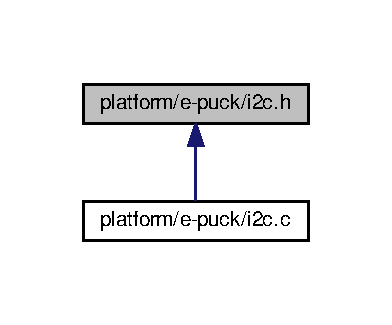
\includegraphics[width=188pt]{d3/df7/i2c_8h__dep__incl}
\end{center}
\end{figure}
\subsection*{Functions}
\begin{DoxyCompactItemize}
\item 
void \hyperlink{i2c_8h_ae0e15cb80a0603c250857c1a799a62f5}{Sys\+\_\+\+Init\+\_\+\+I2\+C} (void)
\item 
void \hyperlink{i2c_8h_a47a8891b8d4ec015d28d2fb38db7af81}{Sys\+\_\+\+Start\+\_\+\+I2\+C} (void)
\item 
void \hyperlink{i2c_8h_a5093f0861938b0821984309c08ed245a}{Sys\+\_\+\+Pause\+\_\+\+I2\+C} (void)
\item 
void \hyperlink{i2c_8h_afd7fe98d1cae4221b8541e2f232a1fe8}{Sys\+\_\+\+Contine\+\_\+\+I2\+C} (void)
\item 
void \hyperlink{i2c_8h_a808f963da209bf3a2437be9ac98b3ae3}{Sys\+\_\+\+Stop\+\_\+\+I2\+C} (void)
\item 
void \hyperlink{i2c_8h_ad333b7abeb87e8f8c18d3dedd031ad5c}{Sys\+\_\+\+I2\+C\+\_\+\+Sent\+Bytes} (\hyperlink{definitions_8h_adde6aaee8457bee49c2a92621fe22b79}{uint8} address, \hyperlink{definitions_8h_adde6aaee8457bee49c2a92621fe22b79}{uint8} $\ast$bytes, \hyperlink{definitions_8h_a05f6b0ae8f6a6e135b0e290c25fe0e4e}{uint16} length)
\item 
void \hyperlink{i2c_8h_ab85476756c65b454eea96255916e22f9}{Sys\+\_\+\+I2\+C\+\_\+\+Read} (\hyperlink{definitions_8h_adde6aaee8457bee49c2a92621fe22b79}{uint8} address, \hyperlink{definitions_8h_adde6aaee8457bee49c2a92621fe22b79}{uint8} $\ast$intern\+\_\+address, \hyperlink{definitions_8h_a05f6b0ae8f6a6e135b0e290c25fe0e4e}{uint16} length, \hyperlink{definitions_8h_a82fa7f76266ee1d687b76a44445f21ef}{p\+Byte\+Function} bytehandler)
\end{DoxyCompactItemize}


\subsection{Detailed Description}
This file includes functions to read and write on the I2\+C interface. 

\begin{DoxyAuthor}{Author}
Stefan M. Trenkwalder \href{mailto:s.trenkwalder@openswarm.org}{\tt s.\+trenkwalder@openswarm.\+org} 
\end{DoxyAuthor}
\begin{DoxyVersion}{Version}
1.\+0
\end{DoxyVersion}
\begin{DoxyDate}{Date}
10 August 2015
\end{DoxyDate}
\begin{DoxyCopyright}{Copyright}
adapted Free\+B\+S\+D License (see \href{http://openswarm.org/license}{\tt http\+://openswarm.\+org/license}) 
\end{DoxyCopyright}


\subsection{Function Documentation}
\hypertarget{i2c_8h_afd7fe98d1cae4221b8541e2f232a1fe8}{}\index{i2c.\+h@{i2c.\+h}!Sys\+\_\+\+Contine\+\_\+\+I2\+C@{Sys\+\_\+\+Contine\+\_\+\+I2\+C}}
\index{Sys\+\_\+\+Contine\+\_\+\+I2\+C@{Sys\+\_\+\+Contine\+\_\+\+I2\+C}!i2c.\+h@{i2c.\+h}}
\subsubsection[{Sys\+\_\+\+Contine\+\_\+\+I2\+C}]{\setlength{\rightskip}{0pt plus 5cm}void Sys\+\_\+\+Contine\+\_\+\+I2\+C (
\begin{DoxyParamCaption}
\item[{void}]{}
\end{DoxyParamCaption}
)\hspace{0.3cm}{\ttfamily [inline]}}\label{i2c_8h_afd7fe98d1cae4221b8541e2f232a1fe8}
continues the I2\+C interface

This function continues the I2\+C interface. 

Definition at line 72 of file i2c.\+c.

\hypertarget{i2c_8h_ab85476756c65b454eea96255916e22f9}{}\index{i2c.\+h@{i2c.\+h}!Sys\+\_\+\+I2\+C\+\_\+\+Read@{Sys\+\_\+\+I2\+C\+\_\+\+Read}}
\index{Sys\+\_\+\+I2\+C\+\_\+\+Read@{Sys\+\_\+\+I2\+C\+\_\+\+Read}!i2c.\+h@{i2c.\+h}}
\subsubsection[{Sys\+\_\+\+I2\+C\+\_\+\+Read}]{\setlength{\rightskip}{0pt plus 5cm}void Sys\+\_\+\+I2\+C\+\_\+\+Read (
\begin{DoxyParamCaption}
\item[{{\bf uint8}}]{address, }
\item[{{\bf uint8} $\ast$}]{intern\+\_\+address, }
\item[{{\bf uint16}}]{length, }
\item[{{\bf p\+Byte\+Function}}]{bytehandler}
\end{DoxyParamCaption}
)}\label{i2c_8h_ab85476756c65b454eea96255916e22f9}
reads bytes from an I2\+C device

This function first sends a reading request to the I2\+C device and, then, handles the incoming bytes with a callback function.


\begin{DoxyParams}[1]{Parameters}
\mbox{\tt in}  & {\em address} & The address of the I2\+C device that should receive the request \\
\hline
\mbox{\tt in}  & {\em intern\+\_\+address} & A pointer to the address which should be read \\
\hline
\mbox{\tt in}  & {\em length} & the number of bytes of the address \\
\hline
\mbox{\tt in}  & {\em bytehandler} & a pointer to the handler function that processes the incoming bytes. \\
\hline
\end{DoxyParams}


Definition at line 367 of file i2c.\+c.

\hypertarget{i2c_8h_ad333b7abeb87e8f8c18d3dedd031ad5c}{}\index{i2c.\+h@{i2c.\+h}!Sys\+\_\+\+I2\+C\+\_\+\+Sent\+Bytes@{Sys\+\_\+\+I2\+C\+\_\+\+Sent\+Bytes}}
\index{Sys\+\_\+\+I2\+C\+\_\+\+Sent\+Bytes@{Sys\+\_\+\+I2\+C\+\_\+\+Sent\+Bytes}!i2c.\+h@{i2c.\+h}}
\subsubsection[{Sys\+\_\+\+I2\+C\+\_\+\+Sent\+Bytes}]{\setlength{\rightskip}{0pt plus 5cm}void Sys\+\_\+\+I2\+C\+\_\+\+Sent\+Bytes (
\begin{DoxyParamCaption}
\item[{{\bf uint8}}]{address, }
\item[{{\bf uint8} $\ast$}]{bytes, }
\item[{{\bf uint16}}]{length}
\end{DoxyParamCaption}
)}\label{i2c_8h_ad333b7abeb87e8f8c18d3dedd031ad5c}
adds bytes into a writing buffer

This function adds bytes into a writing buffer that are written as soon as the I2\+C is idle.

\begin{DoxyNote}{Note}
all bytes are written in sequence 
\end{DoxyNote}

\begin{DoxyParams}[1]{Parameters}
\mbox{\tt in}  & {\em address} & The address of the I2\+C device that should receive the data \\
\hline
\mbox{\tt in}  & {\em bytes} & A pointer to the data which should be sent \\
\hline
\mbox{\tt in}  & {\em length} & the number of bytes to send \\
\hline
\end{DoxyParams}


Definition at line 341 of file i2c.\+c.

\hypertarget{i2c_8h_ae0e15cb80a0603c250857c1a799a62f5}{}\index{i2c.\+h@{i2c.\+h}!Sys\+\_\+\+Init\+\_\+\+I2\+C@{Sys\+\_\+\+Init\+\_\+\+I2\+C}}
\index{Sys\+\_\+\+Init\+\_\+\+I2\+C@{Sys\+\_\+\+Init\+\_\+\+I2\+C}!i2c.\+h@{i2c.\+h}}
\subsubsection[{Sys\+\_\+\+Init\+\_\+\+I2\+C}]{\setlength{\rightskip}{0pt plus 5cm}void Sys\+\_\+\+Init\+\_\+\+I2\+C (
\begin{DoxyParamCaption}
\item[{void}]{}
\end{DoxyParamCaption}
)\hspace{0.3cm}{\ttfamily [inline]}}\label{i2c_8h_ae0e15cb80a0603c250857c1a799a62f5}
Initialises the I2\+C interface

This function initialises the I2\+C interface. 

Definition at line 42 of file i2c.\+c.

\hypertarget{i2c_8h_a5093f0861938b0821984309c08ed245a}{}\index{i2c.\+h@{i2c.\+h}!Sys\+\_\+\+Pause\+\_\+\+I2\+C@{Sys\+\_\+\+Pause\+\_\+\+I2\+C}}
\index{Sys\+\_\+\+Pause\+\_\+\+I2\+C@{Sys\+\_\+\+Pause\+\_\+\+I2\+C}!i2c.\+h@{i2c.\+h}}
\subsubsection[{Sys\+\_\+\+Pause\+\_\+\+I2\+C}]{\setlength{\rightskip}{0pt plus 5cm}void Sys\+\_\+\+Pause\+\_\+\+I2\+C (
\begin{DoxyParamCaption}
\item[{void}]{}
\end{DoxyParamCaption}
)\hspace{0.3cm}{\ttfamily [inline]}}\label{i2c_8h_a5093f0861938b0821984309c08ed245a}
pauses the I2\+C interface

This function pauses the I2\+C interface. 

Definition at line 62 of file i2c.\+c.

\hypertarget{i2c_8h_a47a8891b8d4ec015d28d2fb38db7af81}{}\index{i2c.\+h@{i2c.\+h}!Sys\+\_\+\+Start\+\_\+\+I2\+C@{Sys\+\_\+\+Start\+\_\+\+I2\+C}}
\index{Sys\+\_\+\+Start\+\_\+\+I2\+C@{Sys\+\_\+\+Start\+\_\+\+I2\+C}!i2c.\+h@{i2c.\+h}}
\subsubsection[{Sys\+\_\+\+Start\+\_\+\+I2\+C}]{\setlength{\rightskip}{0pt plus 5cm}void Sys\+\_\+\+Start\+\_\+\+I2\+C (
\begin{DoxyParamCaption}
\item[{void}]{}
\end{DoxyParamCaption}
)\hspace{0.3cm}{\ttfamily [inline]}}\label{i2c_8h_a47a8891b8d4ec015d28d2fb38db7af81}
Starts the I2\+C interface

This function starts the I2\+C interface. 

Definition at line 52 of file i2c.\+c.

\hypertarget{i2c_8h_a808f963da209bf3a2437be9ac98b3ae3}{}\index{i2c.\+h@{i2c.\+h}!Sys\+\_\+\+Stop\+\_\+\+I2\+C@{Sys\+\_\+\+Stop\+\_\+\+I2\+C}}
\index{Sys\+\_\+\+Stop\+\_\+\+I2\+C@{Sys\+\_\+\+Stop\+\_\+\+I2\+C}!i2c.\+h@{i2c.\+h}}
\subsubsection[{Sys\+\_\+\+Stop\+\_\+\+I2\+C}]{\setlength{\rightskip}{0pt plus 5cm}void Sys\+\_\+\+Stop\+\_\+\+I2\+C (
\begin{DoxyParamCaption}
\item[{void}]{}
\end{DoxyParamCaption}
)\hspace{0.3cm}{\ttfamily [inline]}}\label{i2c_8h_a808f963da209bf3a2437be9ac98b3ae3}
stops the I2\+C interface

This function stops the I2\+C interface. 

Definition at line 82 of file i2c.\+c.


\hypertarget{i2c__data_8c}{}\section{platform/e-\/puck/i2c\+\_\+data.c File Reference}
\label{i2c__data_8c}\index{platform/e-\/puck/i2c\+\_\+data.\+c@{platform/e-\/puck/i2c\+\_\+data.\+c}}


defines functions to manage the I2\+C queue.  


{\ttfamily \#include \char`\"{}i2c\+\_\+data.\+h\char`\"{}}\\*
{\ttfamily \#include \char`\"{}../../definitions.\+h\char`\"{}}\\*
{\ttfamily \#include \char`\"{}../../memory.\+h\char`\"{}}\\*
Include dependency graph for i2c\+\_\+data.\+c\+:
\nopagebreak
\begin{figure}[H]
\begin{center}
\leavevmode
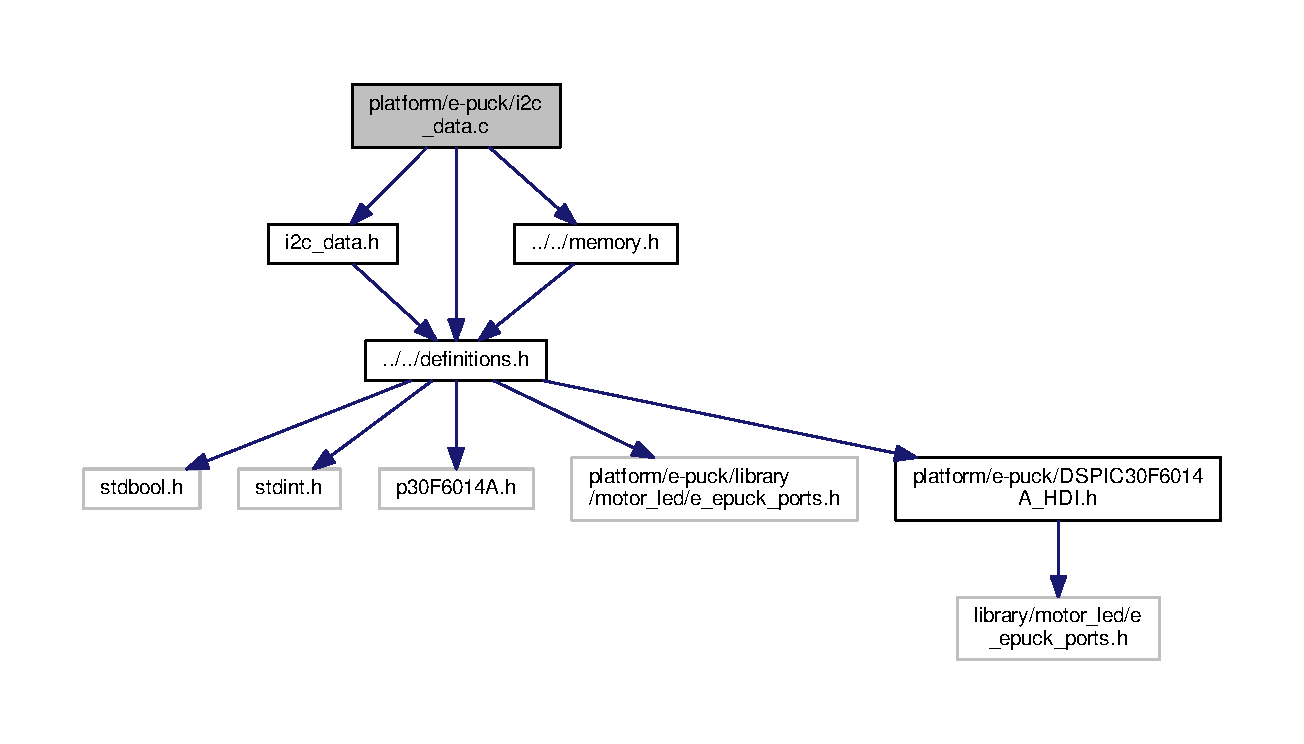
\includegraphics[width=350pt]{d3/d9e/i2c__data_8c__incl}
\end{center}
\end{figure}
\subsection*{Functions}
\begin{DoxyCompactItemize}
\item 
void \hyperlink{i2c__data_8c_aab570c7924073daf517967958aba4250}{Sys\+\_\+\+I2\+C\+\_\+\+Remove\+Oldest\+Message} (\hyperlink{i2c__data_8h_a27b7f72b53024ca33a713e12d9c5a5b6}{sys\+\_\+i2c\+\_\+messages} $\ast$$\ast$list)
\item 
void \hyperlink{i2c__data_8c_a11867d2a3620c96f6a9621f246939a28}{Sys\+\_\+\+I2\+C\+\_\+\+Free\+Messages} (\hyperlink{i2c__data_8h_a27b7f72b53024ca33a713e12d9c5a5b6}{sys\+\_\+i2c\+\_\+messages} $\ast$list)
\item 
void \hyperlink{i2c__data_8c_a37ea66b4bc94c628d177842936370926}{Sys\+\_\+\+I2\+C\+\_\+\+Append\+Messages} (\hyperlink{i2c__data_8h_a63103d69a23446aa735d85acef1936bf}{sys\+\_\+i2c\+\_\+msg} $\ast$item)
\end{DoxyCompactItemize}
\subsection*{Variables}
\begin{DoxyCompactItemize}
\item 
\hyperlink{i2c__data_8h_a27b7f72b53024ca33a713e12d9c5a5b6}{sys\+\_\+i2c\+\_\+messages} $\ast$ \hyperlink{i2c__data_8c_ab06ea00913c00acfd046536bef96a344}{sys\+\_\+i2c\+\_\+msgs} = 0
\end{DoxyCompactItemize}


\subsection{Detailed Description}
defines functions to manage the I2\+C queue. 

\begin{DoxyAuthor}{Author}
Stefan M. Trenkwalder \href{mailto:s.trenkwalder@openswarm.org}{\tt s.\+trenkwalder@openswarm.\+org} 
\end{DoxyAuthor}
\begin{DoxyVersion}{Version}
1.\+0
\end{DoxyVersion}
\begin{DoxyDate}{Date}
10 August 2015
\end{DoxyDate}
\begin{DoxyCopyright}{Copyright}
adapted Free\+B\+S\+D License (see \href{http://openswarm.org/license}{\tt http\+://openswarm.\+org/license}) 
\end{DoxyCopyright}


\subsection{Function Documentation}
\hypertarget{i2c__data_8c_a37ea66b4bc94c628d177842936370926}{}\index{i2c\+\_\+data.\+c@{i2c\+\_\+data.\+c}!Sys\+\_\+\+I2\+C\+\_\+\+Append\+Messages@{Sys\+\_\+\+I2\+C\+\_\+\+Append\+Messages}}
\index{Sys\+\_\+\+I2\+C\+\_\+\+Append\+Messages@{Sys\+\_\+\+I2\+C\+\_\+\+Append\+Messages}!i2c\+\_\+data.\+c@{i2c\+\_\+data.\+c}}
\subsubsection[{Sys\+\_\+\+I2\+C\+\_\+\+Append\+Messages}]{\setlength{\rightskip}{0pt plus 5cm}void Sys\+\_\+\+I2\+C\+\_\+\+Append\+Messages (
\begin{DoxyParamCaption}
\item[{{\bf sys\+\_\+i2c\+\_\+msg} $\ast$}]{item}
\end{DoxyParamCaption}
)}\label{i2c__data_8c_a37ea66b4bc94c628d177842936370926}
appends an element to the linked list.

This function appends on the bottom of the linked list.


\begin{DoxyParams}[1]{Parameters}
\mbox{\tt in,out}  & {\em item} & pointer to a element that should be added \\
\hline
\end{DoxyParams}


Definition at line 69 of file i2c\+\_\+data.\+c.

\hypertarget{i2c__data_8c_a11867d2a3620c96f6a9621f246939a28}{}\index{i2c\+\_\+data.\+c@{i2c\+\_\+data.\+c}!Sys\+\_\+\+I2\+C\+\_\+\+Free\+Messages@{Sys\+\_\+\+I2\+C\+\_\+\+Free\+Messages}}
\index{Sys\+\_\+\+I2\+C\+\_\+\+Free\+Messages@{Sys\+\_\+\+I2\+C\+\_\+\+Free\+Messages}!i2c\+\_\+data.\+c@{i2c\+\_\+data.\+c}}
\subsubsection[{Sys\+\_\+\+I2\+C\+\_\+\+Free\+Messages}]{\setlength{\rightskip}{0pt plus 5cm}void Sys\+\_\+\+I2\+C\+\_\+\+Free\+Messages (
\begin{DoxyParamCaption}
\item[{{\bf sys\+\_\+i2c\+\_\+messages} $\ast$}]{list}
\end{DoxyParamCaption}
)}\label{i2c__data_8c_a11867d2a3620c96f6a9621f246939a28}
frees all messages of the linked list

This function frees all messages of the linked list.


\begin{DoxyParams}[1]{Parameters}
\mbox{\tt in}  & {\em list} & pointer to a list of elements that should be removed \\
\hline
\end{DoxyParams}


Definition at line 47 of file i2c\+\_\+data.\+c.

\hypertarget{i2c__data_8c_aab570c7924073daf517967958aba4250}{}\index{i2c\+\_\+data.\+c@{i2c\+\_\+data.\+c}!Sys\+\_\+\+I2\+C\+\_\+\+Remove\+Oldest\+Message@{Sys\+\_\+\+I2\+C\+\_\+\+Remove\+Oldest\+Message}}
\index{Sys\+\_\+\+I2\+C\+\_\+\+Remove\+Oldest\+Message@{Sys\+\_\+\+I2\+C\+\_\+\+Remove\+Oldest\+Message}!i2c\+\_\+data.\+c@{i2c\+\_\+data.\+c}}
\subsubsection[{Sys\+\_\+\+I2\+C\+\_\+\+Remove\+Oldest\+Message}]{\setlength{\rightskip}{0pt plus 5cm}void Sys\+\_\+\+I2\+C\+\_\+\+Remove\+Oldest\+Message (
\begin{DoxyParamCaption}
\item[{{\bf sys\+\_\+i2c\+\_\+messages} $\ast$$\ast$}]{list}
\end{DoxyParamCaption}
)}\label{i2c__data_8c_aab570c7924073daf517967958aba4250}
removes oldest message from the linked list

This function removes the oldest message (first element) of the linked list


\begin{DoxyParams}[1]{Parameters}
\mbox{\tt in,out}  & {\em list} & pointer to the linked list \\
\hline
\end{DoxyParams}


Definition at line 30 of file i2c\+\_\+data.\+c.



\subsection{Variable Documentation}
\hypertarget{i2c__data_8c_ab06ea00913c00acfd046536bef96a344}{}\index{i2c\+\_\+data.\+c@{i2c\+\_\+data.\+c}!sys\+\_\+i2c\+\_\+msgs@{sys\+\_\+i2c\+\_\+msgs}}
\index{sys\+\_\+i2c\+\_\+msgs@{sys\+\_\+i2c\+\_\+msgs}!i2c\+\_\+data.\+c@{i2c\+\_\+data.\+c}}
\subsubsection[{sys\+\_\+i2c\+\_\+msgs}]{\setlength{\rightskip}{0pt plus 5cm}{\bf sys\+\_\+i2c\+\_\+messages}$\ast$ sys\+\_\+i2c\+\_\+msgs = 0}\label{i2c__data_8c_ab06ea00913c00acfd046536bef96a344}
Pointer to the linked list of messages 

Definition at line 21 of file i2c\+\_\+data.\+c.


\hypertarget{i2c__data_8h}{}\subsection{platform/e-\/puck/i2c\+\_\+data.h File Reference}
\label{i2c__data_8h}\index{platform/e-\/puck/i2c\+\_\+data.\+h@{platform/e-\/puck/i2c\+\_\+data.\+h}}


It declares functions to manage the I2\+C queue.  


{\ttfamily \#include \char`\"{}../../definitions.\+h\char`\"{}}\\*
Include dependency graph for i2c\+\_\+data.\+h\+:\nopagebreak
\begin{figure}[H]
\begin{center}
\leavevmode
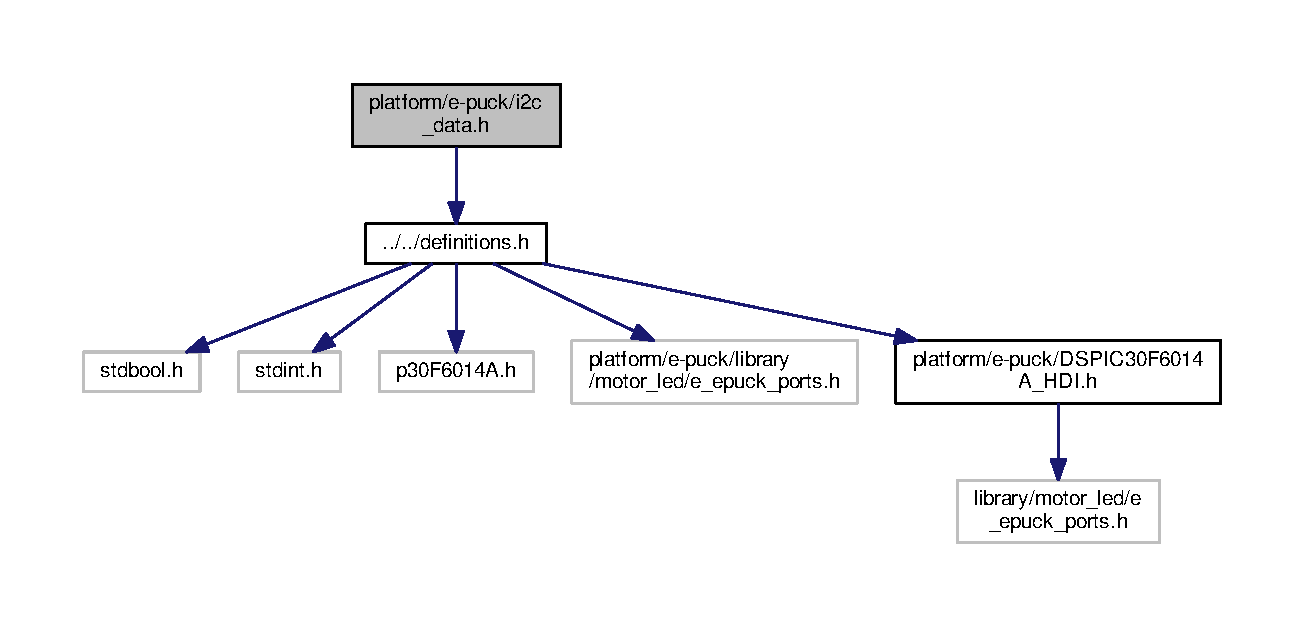
\includegraphics[width=350pt]{d5/ddf/i2c__data_8h__incl}
\end{center}
\end{figure}
This graph shows which files directly or indirectly include this file\+:\nopagebreak
\begin{figure}[H]
\begin{center}
\leavevmode
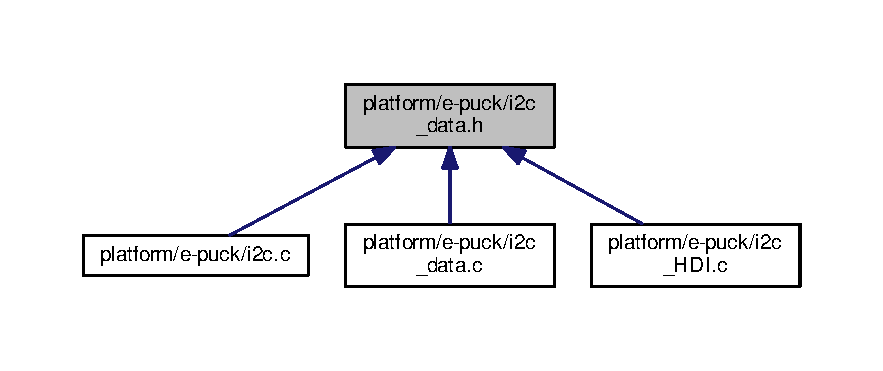
\includegraphics[width=350pt]{d0/de9/i2c__data_8h__dep__incl}
\end{center}
\end{figure}
\subsubsection*{Data Structures}
\begin{DoxyCompactItemize}
\item 
struct \hyperlink{structsys__i2c__msg}{sys\+\_\+i2c\+\_\+msg}
\begin{DoxyCompactList}\small\item\em It is a single linked list element containing messages that need to be sent via I2\+C. This list acts as a message buffer. \end{DoxyCompactList}\end{DoxyCompactItemize}
\subsubsection*{Enumerations}
\begin{DoxyCompactItemize}
\item 
enum \hyperlink{i2c__data_8h_aaea896519531b1b103f1c379945cf84f}{sys\+\_\+\+I2\+C\+\_\+state} \{ \\*
\hyperlink{i2c__data_8h_aaea896519531b1b103f1c379945cf84fa7810297ccb052132c025d8038759159e}{I2\+C\+\_\+\+I\+D\+L\+E} = 0, 
\hyperlink{i2c__data_8h_aaea896519531b1b103f1c379945cf84fa173659288d0f90695fa351dae6feb96b}{I2\+C\+\_\+\+I\+S\+\_\+\+S\+T\+A\+R\+T\+I\+N\+G}, 
\hyperlink{i2c__data_8h_aaea896519531b1b103f1c379945cf84fa6afffe631c354782bca82189eed56936}{I2\+C\+\_\+\+S\+T\+A\+R\+T\+E\+D}, 
\hyperlink{i2c__data_8h_aaea896519531b1b103f1c379945cf84fa5afe3d6f18faf703105d9c5d2fddf0b3}{I2\+C\+\_\+\+I\+S\+\_\+\+R\+E\+A\+D\+I\+N\+G}, 
\\*
\hyperlink{i2c__data_8h_aaea896519531b1b103f1c379945cf84fab3d4495decdac5ea39289dc517be74ec}{I2\+C\+\_\+\+I\+S\+\_\+\+S\+E\+N\+D\+I\+N\+G}, 
\hyperlink{i2c__data_8h_aaea896519531b1b103f1c379945cf84fa04acad9a2e277c0dc73e52dfa554ea23}{I2\+C\+\_\+\+S\+E\+N\+T}, 
\hyperlink{i2c__data_8h_aaea896519531b1b103f1c379945cf84fabdaaa92cbe9cb268c45f3bbd847c43d6}{I2\+C\+\_\+\+A\+C\+K\+N\+O\+W\+L\+E\+D\+G\+E\+D}, 
\hyperlink{i2c__data_8h_aaea896519531b1b103f1c379945cf84fa42a2a9748b25af1d7e1abfcb2a34d99a}{I2\+C\+\_\+\+I\+S\+\_\+\+S\+T\+O\+P\+P\+I\+N\+G}, 
\\*
\hyperlink{i2c__data_8h_aaea896519531b1b103f1c379945cf84fa2e4932a1868432bff23103fac0127fdc}{I2\+C\+\_\+\+E\+R\+R\+O\+R}
 \}
\item 
enum \hyperlink{i2c__data_8h_a85128b419fb98b83541abe5a09898bd0}{sys\+\_\+\+I2\+C\+\_\+mode} \{ \\*
\hyperlink{i2c__data_8h_a85128b419fb98b83541abe5a09898bd0a29f9afef2b8435a81ccd65d3b5ec9021}{I2\+C\+\_\+\+I\+D\+L\+E\+\_\+\+M\+O\+D\+E} = 0, 
\hyperlink{i2c__data_8h_a85128b419fb98b83541abe5a09898bd0aa2577c2ef706dc6500bf1a3680438dcd}{I2\+C\+\_\+\+W\+R\+I\+T\+I\+N\+G\+\_\+\+A\+D\+D\+R\+E\+S\+S\+\_\+\+M\+O\+D\+E}, 
\hyperlink{i2c__data_8h_a85128b419fb98b83541abe5a09898bd0ad96dbed0271c27ac3fd938ac434d31c2}{I2\+C\+\_\+\+R\+E\+A\+D\+I\+N\+G\+\_\+\+B\+Y\+T\+E\+S\+\_\+\+M\+O\+D\+E}, 
\hyperlink{i2c__data_8h_a85128b419fb98b83541abe5a09898bd0a24bc37b846d00fc16234a2e0c3ea4024}{I2\+C\+\_\+\+W\+R\+I\+T\+I\+N\+G\+\_\+\+B\+Y\+T\+E\+S\+\_\+\+M\+O\+D\+E}, 
\\*
\hyperlink{i2c__data_8h_a85128b419fb98b83541abe5a09898bd0ac37fa0c432538664d82d2d282e56dc4b}{I2\+C\+\_\+\+E\+R\+R\+O\+R\+\_\+\+M\+O\+D\+E}
 \}
\end{DoxyCompactItemize}
\subsubsection*{Functions}
\begin{DoxyCompactItemize}
\item 
void \hyperlink{i2c__data_8h_a37ea66b4bc94c628d177842936370926}{Sys\+\_\+\+I2\+C\+\_\+\+Append\+Messages} (\hyperlink{structsys__i2c__msg}{sys\+\_\+i2c\+\_\+msg} $\ast$item)
\item 
void \hyperlink{i2c__data_8h_aab570c7924073daf517967958aba4250}{Sys\+\_\+\+I2\+C\+\_\+\+Remove\+Oldest\+Message} (sys\+\_\+i2c\+\_\+messages $\ast$$\ast$list)
\item 
void \hyperlink{i2c__data_8h_a11867d2a3620c96f6a9621f246939a28}{Sys\+\_\+\+I2\+C\+\_\+\+Free\+Messages} (sys\+\_\+i2c\+\_\+messages $\ast$list)
\end{DoxyCompactItemize}
\subsubsection*{Variables}
\begin{DoxyCompactItemize}
\item 
sys\+\_\+i2c\+\_\+messages $\ast$ \hyperlink{i2c__data_8h_ab06ea00913c00acfd046536bef96a344}{sys\+\_\+i2c\+\_\+msgs}
\end{DoxyCompactItemize}


\subsubsection{Detailed Description}
It declares functions to manage the I2\+C queue. 

\begin{DoxyAuthor}{Author}
Stefan M. Trenkwalder \href{mailto:s.trenkwalder@openswarm.org}{\tt s.\+trenkwalder@openswarm.\+org} 
\end{DoxyAuthor}
\begin{DoxyVersion}{Version}
1.\+0
\end{DoxyVersion}
\begin{DoxyDate}{Date}
10 August 2015
\end{DoxyDate}
\begin{DoxyCopyright}{Copyright}
adapted Free\+B\+S\+D License (see \href{http://openswarm.org/license}{\tt http\+://openswarm.\+org/license}) 
\end{DoxyCopyright}


\subsubsection{Enumeration Type Documentation}
\hypertarget{i2c__data_8h_a85128b419fb98b83541abe5a09898bd0}{}\index{i2c\+\_\+data.\+h@{i2c\+\_\+data.\+h}!sys\+\_\+\+I2\+C\+\_\+mode@{sys\+\_\+\+I2\+C\+\_\+mode}}
\index{sys\+\_\+\+I2\+C\+\_\+mode@{sys\+\_\+\+I2\+C\+\_\+mode}!i2c\+\_\+data.\+h@{i2c\+\_\+data.\+h}}
\paragraph[{sys\+\_\+\+I2\+C\+\_\+mode}]{\setlength{\rightskip}{0pt plus 5cm}enum {\bf sys\+\_\+\+I2\+C\+\_\+mode}}\label{i2c__data_8h_a85128b419fb98b83541abe5a09898bd0}
\begin{Desc}
\item[Enumerator]\par
\begin{description}
\index{I2\+C\+\_\+\+I\+D\+L\+E\+\_\+\+M\+O\+D\+E@{I2\+C\+\_\+\+I\+D\+L\+E\+\_\+\+M\+O\+D\+E}!i2c\+\_\+data.\+h@{i2c\+\_\+data.\+h}}\index{i2c\+\_\+data.\+h@{i2c\+\_\+data.\+h}!I2\+C\+\_\+\+I\+D\+L\+E\+\_\+\+M\+O\+D\+E@{I2\+C\+\_\+\+I\+D\+L\+E\+\_\+\+M\+O\+D\+E}}\item[{\em 
\hypertarget{i2c__data_8h_a85128b419fb98b83541abe5a09898bd0a29f9afef2b8435a81ccd65d3b5ec9021}{}I2\+C\+\_\+\+I\+D\+L\+E\+\_\+\+M\+O\+D\+E\label{i2c__data_8h_a85128b419fb98b83541abe5a09898bd0a29f9afef2b8435a81ccd65d3b5ec9021}
}]\index{I2\+C\+\_\+\+W\+R\+I\+T\+I\+N\+G\+\_\+\+A\+D\+D\+R\+E\+S\+S\+\_\+\+M\+O\+D\+E@{I2\+C\+\_\+\+W\+R\+I\+T\+I\+N\+G\+\_\+\+A\+D\+D\+R\+E\+S\+S\+\_\+\+M\+O\+D\+E}!i2c\+\_\+data.\+h@{i2c\+\_\+data.\+h}}\index{i2c\+\_\+data.\+h@{i2c\+\_\+data.\+h}!I2\+C\+\_\+\+W\+R\+I\+T\+I\+N\+G\+\_\+\+A\+D\+D\+R\+E\+S\+S\+\_\+\+M\+O\+D\+E@{I2\+C\+\_\+\+W\+R\+I\+T\+I\+N\+G\+\_\+\+A\+D\+D\+R\+E\+S\+S\+\_\+\+M\+O\+D\+E}}\item[{\em 
\hypertarget{i2c__data_8h_a85128b419fb98b83541abe5a09898bd0aa2577c2ef706dc6500bf1a3680438dcd}{}I2\+C\+\_\+\+W\+R\+I\+T\+I\+N\+G\+\_\+\+A\+D\+D\+R\+E\+S\+S\+\_\+\+M\+O\+D\+E\label{i2c__data_8h_a85128b419fb98b83541abe5a09898bd0aa2577c2ef706dc6500bf1a3680438dcd}
}]\index{I2\+C\+\_\+\+R\+E\+A\+D\+I\+N\+G\+\_\+\+B\+Y\+T\+E\+S\+\_\+\+M\+O\+D\+E@{I2\+C\+\_\+\+R\+E\+A\+D\+I\+N\+G\+\_\+\+B\+Y\+T\+E\+S\+\_\+\+M\+O\+D\+E}!i2c\+\_\+data.\+h@{i2c\+\_\+data.\+h}}\index{i2c\+\_\+data.\+h@{i2c\+\_\+data.\+h}!I2\+C\+\_\+\+R\+E\+A\+D\+I\+N\+G\+\_\+\+B\+Y\+T\+E\+S\+\_\+\+M\+O\+D\+E@{I2\+C\+\_\+\+R\+E\+A\+D\+I\+N\+G\+\_\+\+B\+Y\+T\+E\+S\+\_\+\+M\+O\+D\+E}}\item[{\em 
\hypertarget{i2c__data_8h_a85128b419fb98b83541abe5a09898bd0ad96dbed0271c27ac3fd938ac434d31c2}{}I2\+C\+\_\+\+R\+E\+A\+D\+I\+N\+G\+\_\+\+B\+Y\+T\+E\+S\+\_\+\+M\+O\+D\+E\label{i2c__data_8h_a85128b419fb98b83541abe5a09898bd0ad96dbed0271c27ac3fd938ac434d31c2}
}]\index{I2\+C\+\_\+\+W\+R\+I\+T\+I\+N\+G\+\_\+\+B\+Y\+T\+E\+S\+\_\+\+M\+O\+D\+E@{I2\+C\+\_\+\+W\+R\+I\+T\+I\+N\+G\+\_\+\+B\+Y\+T\+E\+S\+\_\+\+M\+O\+D\+E}!i2c\+\_\+data.\+h@{i2c\+\_\+data.\+h}}\index{i2c\+\_\+data.\+h@{i2c\+\_\+data.\+h}!I2\+C\+\_\+\+W\+R\+I\+T\+I\+N\+G\+\_\+\+B\+Y\+T\+E\+S\+\_\+\+M\+O\+D\+E@{I2\+C\+\_\+\+W\+R\+I\+T\+I\+N\+G\+\_\+\+B\+Y\+T\+E\+S\+\_\+\+M\+O\+D\+E}}\item[{\em 
\hypertarget{i2c__data_8h_a85128b419fb98b83541abe5a09898bd0a24bc37b846d00fc16234a2e0c3ea4024}{}I2\+C\+\_\+\+W\+R\+I\+T\+I\+N\+G\+\_\+\+B\+Y\+T\+E\+S\+\_\+\+M\+O\+D\+E\label{i2c__data_8h_a85128b419fb98b83541abe5a09898bd0a24bc37b846d00fc16234a2e0c3ea4024}
}]\index{I2\+C\+\_\+\+E\+R\+R\+O\+R\+\_\+\+M\+O\+D\+E@{I2\+C\+\_\+\+E\+R\+R\+O\+R\+\_\+\+M\+O\+D\+E}!i2c\+\_\+data.\+h@{i2c\+\_\+data.\+h}}\index{i2c\+\_\+data.\+h@{i2c\+\_\+data.\+h}!I2\+C\+\_\+\+E\+R\+R\+O\+R\+\_\+\+M\+O\+D\+E@{I2\+C\+\_\+\+E\+R\+R\+O\+R\+\_\+\+M\+O\+D\+E}}\item[{\em 
\hypertarget{i2c__data_8h_a85128b419fb98b83541abe5a09898bd0ac37fa0c432538664d82d2d282e56dc4b}{}I2\+C\+\_\+\+E\+R\+R\+O\+R\+\_\+\+M\+O\+D\+E\label{i2c__data_8h_a85128b419fb98b83541abe5a09898bd0ac37fa0c432538664d82d2d282e56dc4b}
}]\end{description}
\end{Desc}


Definition at line 23 of file i2c\+\_\+data.\+h.

\hypertarget{i2c__data_8h_aaea896519531b1b103f1c379945cf84f}{}\index{i2c\+\_\+data.\+h@{i2c\+\_\+data.\+h}!sys\+\_\+\+I2\+C\+\_\+state@{sys\+\_\+\+I2\+C\+\_\+state}}
\index{sys\+\_\+\+I2\+C\+\_\+state@{sys\+\_\+\+I2\+C\+\_\+state}!i2c\+\_\+data.\+h@{i2c\+\_\+data.\+h}}
\paragraph[{sys\+\_\+\+I2\+C\+\_\+state}]{\setlength{\rightskip}{0pt plus 5cm}enum {\bf sys\+\_\+\+I2\+C\+\_\+state}}\label{i2c__data_8h_aaea896519531b1b103f1c379945cf84f}
\begin{Desc}
\item[Enumerator]\par
\begin{description}
\index{I2\+C\+\_\+\+I\+D\+L\+E@{I2\+C\+\_\+\+I\+D\+L\+E}!i2c\+\_\+data.\+h@{i2c\+\_\+data.\+h}}\index{i2c\+\_\+data.\+h@{i2c\+\_\+data.\+h}!I2\+C\+\_\+\+I\+D\+L\+E@{I2\+C\+\_\+\+I\+D\+L\+E}}\item[{\em 
\hypertarget{i2c__data_8h_aaea896519531b1b103f1c379945cf84fa7810297ccb052132c025d8038759159e}{}I2\+C\+\_\+\+I\+D\+L\+E\label{i2c__data_8h_aaea896519531b1b103f1c379945cf84fa7810297ccb052132c025d8038759159e}
}]\index{I2\+C\+\_\+\+I\+S\+\_\+\+S\+T\+A\+R\+T\+I\+N\+G@{I2\+C\+\_\+\+I\+S\+\_\+\+S\+T\+A\+R\+T\+I\+N\+G}!i2c\+\_\+data.\+h@{i2c\+\_\+data.\+h}}\index{i2c\+\_\+data.\+h@{i2c\+\_\+data.\+h}!I2\+C\+\_\+\+I\+S\+\_\+\+S\+T\+A\+R\+T\+I\+N\+G@{I2\+C\+\_\+\+I\+S\+\_\+\+S\+T\+A\+R\+T\+I\+N\+G}}\item[{\em 
\hypertarget{i2c__data_8h_aaea896519531b1b103f1c379945cf84fa173659288d0f90695fa351dae6feb96b}{}I2\+C\+\_\+\+I\+S\+\_\+\+S\+T\+A\+R\+T\+I\+N\+G\label{i2c__data_8h_aaea896519531b1b103f1c379945cf84fa173659288d0f90695fa351dae6feb96b}
}]\index{I2\+C\+\_\+\+S\+T\+A\+R\+T\+E\+D@{I2\+C\+\_\+\+S\+T\+A\+R\+T\+E\+D}!i2c\+\_\+data.\+h@{i2c\+\_\+data.\+h}}\index{i2c\+\_\+data.\+h@{i2c\+\_\+data.\+h}!I2\+C\+\_\+\+S\+T\+A\+R\+T\+E\+D@{I2\+C\+\_\+\+S\+T\+A\+R\+T\+E\+D}}\item[{\em 
\hypertarget{i2c__data_8h_aaea896519531b1b103f1c379945cf84fa6afffe631c354782bca82189eed56936}{}I2\+C\+\_\+\+S\+T\+A\+R\+T\+E\+D\label{i2c__data_8h_aaea896519531b1b103f1c379945cf84fa6afffe631c354782bca82189eed56936}
}]\index{I2\+C\+\_\+\+I\+S\+\_\+\+R\+E\+A\+D\+I\+N\+G@{I2\+C\+\_\+\+I\+S\+\_\+\+R\+E\+A\+D\+I\+N\+G}!i2c\+\_\+data.\+h@{i2c\+\_\+data.\+h}}\index{i2c\+\_\+data.\+h@{i2c\+\_\+data.\+h}!I2\+C\+\_\+\+I\+S\+\_\+\+R\+E\+A\+D\+I\+N\+G@{I2\+C\+\_\+\+I\+S\+\_\+\+R\+E\+A\+D\+I\+N\+G}}\item[{\em 
\hypertarget{i2c__data_8h_aaea896519531b1b103f1c379945cf84fa5afe3d6f18faf703105d9c5d2fddf0b3}{}I2\+C\+\_\+\+I\+S\+\_\+\+R\+E\+A\+D\+I\+N\+G\label{i2c__data_8h_aaea896519531b1b103f1c379945cf84fa5afe3d6f18faf703105d9c5d2fddf0b3}
}]\index{I2\+C\+\_\+\+I\+S\+\_\+\+S\+E\+N\+D\+I\+N\+G@{I2\+C\+\_\+\+I\+S\+\_\+\+S\+E\+N\+D\+I\+N\+G}!i2c\+\_\+data.\+h@{i2c\+\_\+data.\+h}}\index{i2c\+\_\+data.\+h@{i2c\+\_\+data.\+h}!I2\+C\+\_\+\+I\+S\+\_\+\+S\+E\+N\+D\+I\+N\+G@{I2\+C\+\_\+\+I\+S\+\_\+\+S\+E\+N\+D\+I\+N\+G}}\item[{\em 
\hypertarget{i2c__data_8h_aaea896519531b1b103f1c379945cf84fab3d4495decdac5ea39289dc517be74ec}{}I2\+C\+\_\+\+I\+S\+\_\+\+S\+E\+N\+D\+I\+N\+G\label{i2c__data_8h_aaea896519531b1b103f1c379945cf84fab3d4495decdac5ea39289dc517be74ec}
}]\index{I2\+C\+\_\+\+S\+E\+N\+T@{I2\+C\+\_\+\+S\+E\+N\+T}!i2c\+\_\+data.\+h@{i2c\+\_\+data.\+h}}\index{i2c\+\_\+data.\+h@{i2c\+\_\+data.\+h}!I2\+C\+\_\+\+S\+E\+N\+T@{I2\+C\+\_\+\+S\+E\+N\+T}}\item[{\em 
\hypertarget{i2c__data_8h_aaea896519531b1b103f1c379945cf84fa04acad9a2e277c0dc73e52dfa554ea23}{}I2\+C\+\_\+\+S\+E\+N\+T\label{i2c__data_8h_aaea896519531b1b103f1c379945cf84fa04acad9a2e277c0dc73e52dfa554ea23}
}]\index{I2\+C\+\_\+\+A\+C\+K\+N\+O\+W\+L\+E\+D\+G\+E\+D@{I2\+C\+\_\+\+A\+C\+K\+N\+O\+W\+L\+E\+D\+G\+E\+D}!i2c\+\_\+data.\+h@{i2c\+\_\+data.\+h}}\index{i2c\+\_\+data.\+h@{i2c\+\_\+data.\+h}!I2\+C\+\_\+\+A\+C\+K\+N\+O\+W\+L\+E\+D\+G\+E\+D@{I2\+C\+\_\+\+A\+C\+K\+N\+O\+W\+L\+E\+D\+G\+E\+D}}\item[{\em 
\hypertarget{i2c__data_8h_aaea896519531b1b103f1c379945cf84fabdaaa92cbe9cb268c45f3bbd847c43d6}{}I2\+C\+\_\+\+A\+C\+K\+N\+O\+W\+L\+E\+D\+G\+E\+D\label{i2c__data_8h_aaea896519531b1b103f1c379945cf84fabdaaa92cbe9cb268c45f3bbd847c43d6}
}]\index{I2\+C\+\_\+\+I\+S\+\_\+\+S\+T\+O\+P\+P\+I\+N\+G@{I2\+C\+\_\+\+I\+S\+\_\+\+S\+T\+O\+P\+P\+I\+N\+G}!i2c\+\_\+data.\+h@{i2c\+\_\+data.\+h}}\index{i2c\+\_\+data.\+h@{i2c\+\_\+data.\+h}!I2\+C\+\_\+\+I\+S\+\_\+\+S\+T\+O\+P\+P\+I\+N\+G@{I2\+C\+\_\+\+I\+S\+\_\+\+S\+T\+O\+P\+P\+I\+N\+G}}\item[{\em 
\hypertarget{i2c__data_8h_aaea896519531b1b103f1c379945cf84fa42a2a9748b25af1d7e1abfcb2a34d99a}{}I2\+C\+\_\+\+I\+S\+\_\+\+S\+T\+O\+P\+P\+I\+N\+G\label{i2c__data_8h_aaea896519531b1b103f1c379945cf84fa42a2a9748b25af1d7e1abfcb2a34d99a}
}]\index{I2\+C\+\_\+\+E\+R\+R\+O\+R@{I2\+C\+\_\+\+E\+R\+R\+O\+R}!i2c\+\_\+data.\+h@{i2c\+\_\+data.\+h}}\index{i2c\+\_\+data.\+h@{i2c\+\_\+data.\+h}!I2\+C\+\_\+\+E\+R\+R\+O\+R@{I2\+C\+\_\+\+E\+R\+R\+O\+R}}\item[{\em 
\hypertarget{i2c__data_8h_aaea896519531b1b103f1c379945cf84fa2e4932a1868432bff23103fac0127fdc}{}I2\+C\+\_\+\+E\+R\+R\+O\+R\label{i2c__data_8h_aaea896519531b1b103f1c379945cf84fa2e4932a1868432bff23103fac0127fdc}
}]\end{description}
\end{Desc}


Definition at line 22 of file i2c\+\_\+data.\+h.



\subsubsection{Function Documentation}
\hypertarget{i2c__data_8h_a37ea66b4bc94c628d177842936370926}{}\index{i2c\+\_\+data.\+h@{i2c\+\_\+data.\+h}!Sys\+\_\+\+I2\+C\+\_\+\+Append\+Messages@{Sys\+\_\+\+I2\+C\+\_\+\+Append\+Messages}}
\index{Sys\+\_\+\+I2\+C\+\_\+\+Append\+Messages@{Sys\+\_\+\+I2\+C\+\_\+\+Append\+Messages}!i2c\+\_\+data.\+h@{i2c\+\_\+data.\+h}}
\paragraph[{Sys\+\_\+\+I2\+C\+\_\+\+Append\+Messages}]{\setlength{\rightskip}{0pt plus 5cm}void Sys\+\_\+\+I2\+C\+\_\+\+Append\+Messages (
\begin{DoxyParamCaption}
\item[{{\bf sys\+\_\+i2c\+\_\+msg} $\ast$}]{item}
\end{DoxyParamCaption}
)}\label{i2c__data_8h_a37ea66b4bc94c628d177842936370926}
This function appends on the bottom of the linked list.


\begin{DoxyParams}[1]{Parameters}
\mbox{\tt in,out}  & {\em item} & pointer to a element that should be added \\
\hline
\end{DoxyParams}


Definition at line 64 of file i2c\+\_\+data.\+c.

\hypertarget{i2c__data_8h_a11867d2a3620c96f6a9621f246939a28}{}\index{i2c\+\_\+data.\+h@{i2c\+\_\+data.\+h}!Sys\+\_\+\+I2\+C\+\_\+\+Free\+Messages@{Sys\+\_\+\+I2\+C\+\_\+\+Free\+Messages}}
\index{Sys\+\_\+\+I2\+C\+\_\+\+Free\+Messages@{Sys\+\_\+\+I2\+C\+\_\+\+Free\+Messages}!i2c\+\_\+data.\+h@{i2c\+\_\+data.\+h}}
\paragraph[{Sys\+\_\+\+I2\+C\+\_\+\+Free\+Messages}]{\setlength{\rightskip}{0pt plus 5cm}void Sys\+\_\+\+I2\+C\+\_\+\+Free\+Messages (
\begin{DoxyParamCaption}
\item[{sys\+\_\+i2c\+\_\+messages $\ast$}]{list}
\end{DoxyParamCaption}
)}\label{i2c__data_8h_a11867d2a3620c96f6a9621f246939a28}
This function frees all messages of the linked list.


\begin{DoxyParams}[1]{Parameters}
\mbox{\tt in}  & {\em list} & pointer to a list of elements that should be removed \\
\hline
\end{DoxyParams}


Definition at line 43 of file i2c\+\_\+data.\+c.

\hypertarget{i2c__data_8h_aab570c7924073daf517967958aba4250}{}\index{i2c\+\_\+data.\+h@{i2c\+\_\+data.\+h}!Sys\+\_\+\+I2\+C\+\_\+\+Remove\+Oldest\+Message@{Sys\+\_\+\+I2\+C\+\_\+\+Remove\+Oldest\+Message}}
\index{Sys\+\_\+\+I2\+C\+\_\+\+Remove\+Oldest\+Message@{Sys\+\_\+\+I2\+C\+\_\+\+Remove\+Oldest\+Message}!i2c\+\_\+data.\+h@{i2c\+\_\+data.\+h}}
\paragraph[{Sys\+\_\+\+I2\+C\+\_\+\+Remove\+Oldest\+Message}]{\setlength{\rightskip}{0pt plus 5cm}void Sys\+\_\+\+I2\+C\+\_\+\+Remove\+Oldest\+Message (
\begin{DoxyParamCaption}
\item[{sys\+\_\+i2c\+\_\+messages $\ast$$\ast$}]{list}
\end{DoxyParamCaption}
)}\label{i2c__data_8h_aab570c7924073daf517967958aba4250}
This function removes the oldest message (first element) of the linked list


\begin{DoxyParams}[1]{Parameters}
\mbox{\tt in,out}  & {\em list} & pointer to the linked list \\
\hline
\end{DoxyParams}


Definition at line 27 of file i2c\+\_\+data.\+c.



\subsubsection{Variable Documentation}
\hypertarget{i2c__data_8h_ab06ea00913c00acfd046536bef96a344}{}\index{i2c\+\_\+data.\+h@{i2c\+\_\+data.\+h}!sys\+\_\+i2c\+\_\+msgs@{sys\+\_\+i2c\+\_\+msgs}}
\index{sys\+\_\+i2c\+\_\+msgs@{sys\+\_\+i2c\+\_\+msgs}!i2c\+\_\+data.\+h@{i2c\+\_\+data.\+h}}
\paragraph[{sys\+\_\+i2c\+\_\+msgs}]{\setlength{\rightskip}{0pt plus 5cm}sys\+\_\+i2c\+\_\+messages$\ast$ sys\+\_\+i2c\+\_\+msgs}\label{i2c__data_8h_ab06ea00913c00acfd046536bef96a344}
Pointer to the linked list of messages 

Definition at line 19 of file i2c\+\_\+data.\+c.


\hypertarget{i2c__HDI_8c}{}\section{platform/e-\/puck/i2c\+\_\+\+H\+D\+I.c File Reference}
\label{i2c__HDI_8c}\index{platform/e-\/puck/i2c\+\_\+\+H\+D\+I.\+c@{platform/e-\/puck/i2c\+\_\+\+H\+D\+I.\+c}}


Hardware dependent implementations to read and write on the I2\+C interface.  


{\ttfamily \#include \char`\"{}i2c\+\_\+\+H\+D\+I.\+h\char`\"{}}\\*
{\ttfamily \#include \char`\"{}i2c\+\_\+data.\+h\char`\"{}}\\*
{\ttfamily \#include \char`\"{}../../definitions.\+h\char`\"{}}\\*
{\ttfamily \#include \char`\"{}../../interrupts.\+h\char`\"{}}\\*
Include dependency graph for i2c\+\_\+\+H\+D\+I.\+c\+:\nopagebreak
\begin{figure}[H]
\begin{center}
\leavevmode
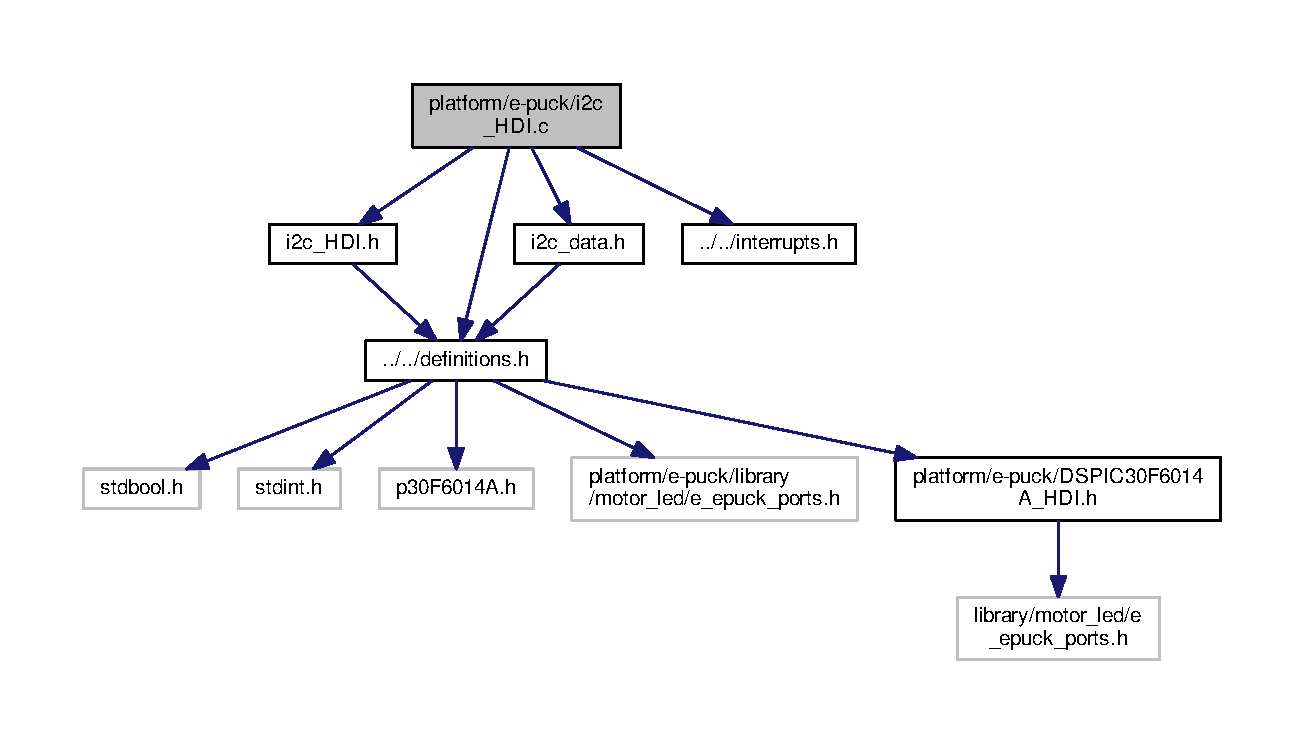
\includegraphics[width=350pt]{d1/d0d/i2c__HDI_8c__incl}
\end{center}
\end{figure}
\subsection*{Functions}
\begin{DoxyCompactItemize}
\item 
void \hyperlink{i2c__HDI_8c_a422894e72364c5671c85dbccc0ece7df}{Sys\+\_\+\+Init\+\_\+\+I2\+C\+\_\+\+H\+D\+I} ()
\item 
void \hyperlink{i2c__HDI_8c_a4c31c5ee2a65479f55423638d9dadf41}{Sys\+\_\+\+Start\+\_\+\+I2\+C\+\_\+\+H\+D\+I} (void)
\item 
void \hyperlink{i2c__HDI_8c_a2952e63416f7336bdd19cbd71bda6168}{Sys\+\_\+\+Pause\+\_\+\+I2\+C\+\_\+\+H\+D\+I} (void)
\item 
void \hyperlink{i2c__HDI_8c_a5b59f613b4a1248bc95646317cb5b7ed}{Sys\+\_\+\+Contine\+\_\+\+I2\+C\+\_\+\+H\+D\+I} (void)
\item 
void \hyperlink{i2c__HDI_8c_a2a09331981865de9c218c6cf5920ff73}{Sys\+\_\+\+Stop\+\_\+\+I2\+C\+\_\+\+H\+D\+I} (void)
\item 
void \hyperlink{i2c__HDI_8c_abf50bdceb354835453ef4650790e9600}{Sys\+\_\+\+I2\+C\+\_\+\+Send\+\_\+\+Start\+\_\+\+H\+D\+I} ()
\item 
void \hyperlink{i2c__HDI_8c_aabc16d13b990930e52593cd5abb41a95}{Sys\+\_\+\+I2\+C\+\_\+\+Send\+\_\+\+Restart\+\_\+\+H\+D\+I} (void)
\item 
void \hyperlink{i2c__HDI_8c_a2d5bb88a3b7dbe61f48234700fdba614}{Sys\+\_\+\+I2\+C\+\_\+\+Send\+\_\+\+Stop\+\_\+\+H\+D\+I} (void)
\item 
void \hyperlink{i2c__HDI_8c_a2994b42ce95e10c422a7998c132c6589}{Sys\+\_\+\+I2\+C\+\_\+\+Send\+\_\+\+A\+C\+K\+\_\+\+H\+D\+I} (void)
\item 
void \hyperlink{i2c__HDI_8c_a7249b63b20eff29ce24e2e5f93a3e7ba}{Sys\+\_\+\+I2\+C\+\_\+\+Send\+\_\+\+N\+A\+C\+K\+\_\+\+H\+D\+I} (void)
\item 
void \hyperlink{i2c__HDI_8c_ae07f975355969f16e6fa71b5195a6832}{Sys\+\_\+\+I2\+C\+\_\+\+Start\+\_\+\+Reading\+\_\+\+H\+D\+I} ()
\item 
char \hyperlink{i2c__HDI_8c_a9ff57299960479781ef856bf61d27233}{Sys\+\_\+\+I2\+C\+\_\+\+Read\+Byte\+\_\+\+H\+D\+I} ()
\item 
void \hyperlink{i2c__HDI_8c_a5941033d2a4855c70e3321f11b846486}{Sys\+\_\+\+I2\+C\+\_\+\+Write\+Byte\+\_\+\+H\+D\+I} (\hyperlink{definitions_8h_adde6aaee8457bee49c2a92621fe22b79}{uint8} byte)
\end{DoxyCompactItemize}


\subsection{Detailed Description}
Hardware dependent implementations to read and write on the I2\+C interface. 

\begin{DoxyAuthor}{Author}
Stefan M. Trenkwalder \href{mailto:s.trenkwalder@openswarm.org}{\tt s.\+trenkwalder@openswarm.\+org} 
\end{DoxyAuthor}
\begin{DoxyVersion}{Version}
1.\+0
\end{DoxyVersion}
\begin{DoxyDate}{Date}
10 August 2015
\end{DoxyDate}
\begin{DoxyCopyright}{Copyright}
adapted Free\+B\+S\+D License (see \href{http://openswarm.org/license}{\tt http\+://openswarm.\+org/license}) 
\end{DoxyCopyright}


\subsection{Function Documentation}
\hypertarget{i2c__HDI_8c_a5b59f613b4a1248bc95646317cb5b7ed}{}\index{i2c\+\_\+\+H\+D\+I.\+c@{i2c\+\_\+\+H\+D\+I.\+c}!Sys\+\_\+\+Contine\+\_\+\+I2\+C\+\_\+\+H\+D\+I@{Sys\+\_\+\+Contine\+\_\+\+I2\+C\+\_\+\+H\+D\+I}}
\index{Sys\+\_\+\+Contine\+\_\+\+I2\+C\+\_\+\+H\+D\+I@{Sys\+\_\+\+Contine\+\_\+\+I2\+C\+\_\+\+H\+D\+I}!i2c\+\_\+\+H\+D\+I.\+c@{i2c\+\_\+\+H\+D\+I.\+c}}
\subsubsection[{Sys\+\_\+\+Contine\+\_\+\+I2\+C\+\_\+\+H\+D\+I}]{\setlength{\rightskip}{0pt plus 5cm}void Sys\+\_\+\+Contine\+\_\+\+I2\+C\+\_\+\+H\+D\+I (
\begin{DoxyParamCaption}
\item[{void}]{}
\end{DoxyParamCaption}
)\hspace{0.3cm}{\ttfamily [inline]}}\label{i2c__HDI_8c_a5b59f613b4a1248bc95646317cb5b7ed}
continues the I2\+C interface

This function continues the I2\+C interface. 

Definition at line 74 of file i2c\+\_\+\+H\+D\+I.\+c.

\hypertarget{i2c__HDI_8c_a9ff57299960479781ef856bf61d27233}{}\index{i2c\+\_\+\+H\+D\+I.\+c@{i2c\+\_\+\+H\+D\+I.\+c}!Sys\+\_\+\+I2\+C\+\_\+\+Read\+Byte\+\_\+\+H\+D\+I@{Sys\+\_\+\+I2\+C\+\_\+\+Read\+Byte\+\_\+\+H\+D\+I}}
\index{Sys\+\_\+\+I2\+C\+\_\+\+Read\+Byte\+\_\+\+H\+D\+I@{Sys\+\_\+\+I2\+C\+\_\+\+Read\+Byte\+\_\+\+H\+D\+I}!i2c\+\_\+\+H\+D\+I.\+c@{i2c\+\_\+\+H\+D\+I.\+c}}
\subsubsection[{Sys\+\_\+\+I2\+C\+\_\+\+Read\+Byte\+\_\+\+H\+D\+I}]{\setlength{\rightskip}{0pt plus 5cm}char Sys\+\_\+\+I2\+C\+\_\+\+Read\+Byte\+\_\+\+H\+D\+I (
\begin{DoxyParamCaption}
\item[{void}]{}
\end{DoxyParamCaption}
)\hspace{0.3cm}{\ttfamily [inline]}}\label{i2c__HDI_8c_a9ff57299960479781ef856bf61d27233}
reads a byte via the I2\+C interface

This function reads a byte. 

Definition at line 178 of file i2c\+\_\+\+H\+D\+I.\+c.

\hypertarget{i2c__HDI_8c_a2994b42ce95e10c422a7998c132c6589}{}\index{i2c\+\_\+\+H\+D\+I.\+c@{i2c\+\_\+\+H\+D\+I.\+c}!Sys\+\_\+\+I2\+C\+\_\+\+Send\+\_\+\+A\+C\+K\+\_\+\+H\+D\+I@{Sys\+\_\+\+I2\+C\+\_\+\+Send\+\_\+\+A\+C\+K\+\_\+\+H\+D\+I}}
\index{Sys\+\_\+\+I2\+C\+\_\+\+Send\+\_\+\+A\+C\+K\+\_\+\+H\+D\+I@{Sys\+\_\+\+I2\+C\+\_\+\+Send\+\_\+\+A\+C\+K\+\_\+\+H\+D\+I}!i2c\+\_\+\+H\+D\+I.\+c@{i2c\+\_\+\+H\+D\+I.\+c}}
\subsubsection[{Sys\+\_\+\+I2\+C\+\_\+\+Send\+\_\+\+A\+C\+K\+\_\+\+H\+D\+I}]{\setlength{\rightskip}{0pt plus 5cm}void Sys\+\_\+\+I2\+C\+\_\+\+Send\+\_\+\+A\+C\+K\+\_\+\+H\+D\+I (
\begin{DoxyParamCaption}
\item[{void}]{}
\end{DoxyParamCaption}
)\hspace{0.3cm}{\ttfamily [inline]}}\label{i2c__HDI_8c_a2994b42ce95e10c422a7998c132c6589}
sends a ack bits via the I2\+C interface

This function sends a ack bits. 

Definition at line 130 of file i2c\+\_\+\+H\+D\+I.\+c.

\hypertarget{i2c__HDI_8c_a7249b63b20eff29ce24e2e5f93a3e7ba}{}\index{i2c\+\_\+\+H\+D\+I.\+c@{i2c\+\_\+\+H\+D\+I.\+c}!Sys\+\_\+\+I2\+C\+\_\+\+Send\+\_\+\+N\+A\+C\+K\+\_\+\+H\+D\+I@{Sys\+\_\+\+I2\+C\+\_\+\+Send\+\_\+\+N\+A\+C\+K\+\_\+\+H\+D\+I}}
\index{Sys\+\_\+\+I2\+C\+\_\+\+Send\+\_\+\+N\+A\+C\+K\+\_\+\+H\+D\+I@{Sys\+\_\+\+I2\+C\+\_\+\+Send\+\_\+\+N\+A\+C\+K\+\_\+\+H\+D\+I}!i2c\+\_\+\+H\+D\+I.\+c@{i2c\+\_\+\+H\+D\+I.\+c}}
\subsubsection[{Sys\+\_\+\+I2\+C\+\_\+\+Send\+\_\+\+N\+A\+C\+K\+\_\+\+H\+D\+I}]{\setlength{\rightskip}{0pt plus 5cm}void Sys\+\_\+\+I2\+C\+\_\+\+Send\+\_\+\+N\+A\+C\+K\+\_\+\+H\+D\+I (
\begin{DoxyParamCaption}
\item[{void}]{}
\end{DoxyParamCaption}
)\hspace{0.3cm}{\ttfamily [inline]}}\label{i2c__HDI_8c_a7249b63b20eff29ce24e2e5f93a3e7ba}
sends a nack bits via the I2\+C interface

This function sends a nack bits. 

Definition at line 146 of file i2c\+\_\+\+H\+D\+I.\+c.

\hypertarget{i2c__HDI_8c_aabc16d13b990930e52593cd5abb41a95}{}\index{i2c\+\_\+\+H\+D\+I.\+c@{i2c\+\_\+\+H\+D\+I.\+c}!Sys\+\_\+\+I2\+C\+\_\+\+Send\+\_\+\+Restart\+\_\+\+H\+D\+I@{Sys\+\_\+\+I2\+C\+\_\+\+Send\+\_\+\+Restart\+\_\+\+H\+D\+I}}
\index{Sys\+\_\+\+I2\+C\+\_\+\+Send\+\_\+\+Restart\+\_\+\+H\+D\+I@{Sys\+\_\+\+I2\+C\+\_\+\+Send\+\_\+\+Restart\+\_\+\+H\+D\+I}!i2c\+\_\+\+H\+D\+I.\+c@{i2c\+\_\+\+H\+D\+I.\+c}}
\subsubsection[{Sys\+\_\+\+I2\+C\+\_\+\+Send\+\_\+\+Restart\+\_\+\+H\+D\+I}]{\setlength{\rightskip}{0pt plus 5cm}void Sys\+\_\+\+I2\+C\+\_\+\+Send\+\_\+\+Restart\+\_\+\+H\+D\+I (
\begin{DoxyParamCaption}
\item[{void}]{}
\end{DoxyParamCaption}
)\hspace{0.3cm}{\ttfamily [inline]}}\label{i2c__HDI_8c_aabc16d13b990930e52593cd5abb41a95}
sends a restart bits via the I2\+C interface

This function sends a restart bits. 

Definition at line 108 of file i2c\+\_\+\+H\+D\+I.\+c.

\hypertarget{i2c__HDI_8c_abf50bdceb354835453ef4650790e9600}{}\index{i2c\+\_\+\+H\+D\+I.\+c@{i2c\+\_\+\+H\+D\+I.\+c}!Sys\+\_\+\+I2\+C\+\_\+\+Send\+\_\+\+Start\+\_\+\+H\+D\+I@{Sys\+\_\+\+I2\+C\+\_\+\+Send\+\_\+\+Start\+\_\+\+H\+D\+I}}
\index{Sys\+\_\+\+I2\+C\+\_\+\+Send\+\_\+\+Start\+\_\+\+H\+D\+I@{Sys\+\_\+\+I2\+C\+\_\+\+Send\+\_\+\+Start\+\_\+\+H\+D\+I}!i2c\+\_\+\+H\+D\+I.\+c@{i2c\+\_\+\+H\+D\+I.\+c}}
\subsubsection[{Sys\+\_\+\+I2\+C\+\_\+\+Send\+\_\+\+Start\+\_\+\+H\+D\+I}]{\setlength{\rightskip}{0pt plus 5cm}void Sys\+\_\+\+I2\+C\+\_\+\+Send\+\_\+\+Start\+\_\+\+H\+D\+I (
\begin{DoxyParamCaption}
{}
\end{DoxyParamCaption}
)\hspace{0.3cm}{\ttfamily [inline]}}\label{i2c__HDI_8c_abf50bdceb354835453ef4650790e9600}
sends a start bits via the I2\+C interface

This function sends a start bits. 

Definition at line 96 of file i2c\+\_\+\+H\+D\+I.\+c.

\hypertarget{i2c__HDI_8c_a2d5bb88a3b7dbe61f48234700fdba614}{}\index{i2c\+\_\+\+H\+D\+I.\+c@{i2c\+\_\+\+H\+D\+I.\+c}!Sys\+\_\+\+I2\+C\+\_\+\+Send\+\_\+\+Stop\+\_\+\+H\+D\+I@{Sys\+\_\+\+I2\+C\+\_\+\+Send\+\_\+\+Stop\+\_\+\+H\+D\+I}}
\index{Sys\+\_\+\+I2\+C\+\_\+\+Send\+\_\+\+Stop\+\_\+\+H\+D\+I@{Sys\+\_\+\+I2\+C\+\_\+\+Send\+\_\+\+Stop\+\_\+\+H\+D\+I}!i2c\+\_\+\+H\+D\+I.\+c@{i2c\+\_\+\+H\+D\+I.\+c}}
\subsubsection[{Sys\+\_\+\+I2\+C\+\_\+\+Send\+\_\+\+Stop\+\_\+\+H\+D\+I}]{\setlength{\rightskip}{0pt plus 5cm}void Sys\+\_\+\+I2\+C\+\_\+\+Send\+\_\+\+Stop\+\_\+\+H\+D\+I (
\begin{DoxyParamCaption}
\item[{void}]{}
\end{DoxyParamCaption}
)\hspace{0.3cm}{\ttfamily [inline]}}\label{i2c__HDI_8c_a2d5bb88a3b7dbe61f48234700fdba614}
sends a stop bits via the I2\+C interface

This function sends a stop bits. 

Definition at line 120 of file i2c\+\_\+\+H\+D\+I.\+c.

\hypertarget{i2c__HDI_8c_ae07f975355969f16e6fa71b5195a6832}{}\index{i2c\+\_\+\+H\+D\+I.\+c@{i2c\+\_\+\+H\+D\+I.\+c}!Sys\+\_\+\+I2\+C\+\_\+\+Start\+\_\+\+Reading\+\_\+\+H\+D\+I@{Sys\+\_\+\+I2\+C\+\_\+\+Start\+\_\+\+Reading\+\_\+\+H\+D\+I}}
\index{Sys\+\_\+\+I2\+C\+\_\+\+Start\+\_\+\+Reading\+\_\+\+H\+D\+I@{Sys\+\_\+\+I2\+C\+\_\+\+Start\+\_\+\+Reading\+\_\+\+H\+D\+I}!i2c\+\_\+\+H\+D\+I.\+c@{i2c\+\_\+\+H\+D\+I.\+c}}
\subsubsection[{Sys\+\_\+\+I2\+C\+\_\+\+Start\+\_\+\+Reading\+\_\+\+H\+D\+I}]{\setlength{\rightskip}{0pt plus 5cm}void Sys\+\_\+\+I2\+C\+\_\+\+Start\+\_\+\+Reading\+\_\+\+H\+D\+I (
\begin{DoxyParamCaption}
\item[{void}]{}
\end{DoxyParamCaption}
)\hspace{0.3cm}{\ttfamily [inline]}}\label{i2c__HDI_8c_ae07f975355969f16e6fa71b5195a6832}
sends a reading bits via the I2\+C interface

This function sends a reading bits. 

Definition at line 162 of file i2c\+\_\+\+H\+D\+I.\+c.

\hypertarget{i2c__HDI_8c_a5941033d2a4855c70e3321f11b846486}{}\index{i2c\+\_\+\+H\+D\+I.\+c@{i2c\+\_\+\+H\+D\+I.\+c}!Sys\+\_\+\+I2\+C\+\_\+\+Write\+Byte\+\_\+\+H\+D\+I@{Sys\+\_\+\+I2\+C\+\_\+\+Write\+Byte\+\_\+\+H\+D\+I}}
\index{Sys\+\_\+\+I2\+C\+\_\+\+Write\+Byte\+\_\+\+H\+D\+I@{Sys\+\_\+\+I2\+C\+\_\+\+Write\+Byte\+\_\+\+H\+D\+I}!i2c\+\_\+\+H\+D\+I.\+c@{i2c\+\_\+\+H\+D\+I.\+c}}
\subsubsection[{Sys\+\_\+\+I2\+C\+\_\+\+Write\+Byte\+\_\+\+H\+D\+I}]{\setlength{\rightskip}{0pt plus 5cm}void Sys\+\_\+\+I2\+C\+\_\+\+Write\+Byte\+\_\+\+H\+D\+I (
\begin{DoxyParamCaption}
\item[{{\bf uint8}}]{byte}
\end{DoxyParamCaption}
)\hspace{0.3cm}{\ttfamily [inline]}}\label{i2c__HDI_8c_a5941033d2a4855c70e3321f11b846486}
writes a byte via the I2\+C interface

This function writes a byte.


\begin{DoxyParams}{Parameters}
{\em byte} & the byte that has to be written \\
\hline
\end{DoxyParams}


Definition at line 189 of file i2c\+\_\+\+H\+D\+I.\+c.

\hypertarget{i2c__HDI_8c_a422894e72364c5671c85dbccc0ece7df}{}\index{i2c\+\_\+\+H\+D\+I.\+c@{i2c\+\_\+\+H\+D\+I.\+c}!Sys\+\_\+\+Init\+\_\+\+I2\+C\+\_\+\+H\+D\+I@{Sys\+\_\+\+Init\+\_\+\+I2\+C\+\_\+\+H\+D\+I}}
\index{Sys\+\_\+\+Init\+\_\+\+I2\+C\+\_\+\+H\+D\+I@{Sys\+\_\+\+Init\+\_\+\+I2\+C\+\_\+\+H\+D\+I}!i2c\+\_\+\+H\+D\+I.\+c@{i2c\+\_\+\+H\+D\+I.\+c}}
\subsubsection[{Sys\+\_\+\+Init\+\_\+\+I2\+C\+\_\+\+H\+D\+I}]{\setlength{\rightskip}{0pt plus 5cm}void Sys\+\_\+\+Init\+\_\+\+I2\+C\+\_\+\+H\+D\+I (
\begin{DoxyParamCaption}
\item[{void}]{}
\end{DoxyParamCaption}
)\hspace{0.3cm}{\ttfamily [inline]}}\label{i2c__HDI_8c_a422894e72364c5671c85dbccc0ece7df}
Initialises the I2\+C interface

This function initialises the I2\+C interface. 

Definition at line 27 of file i2c\+\_\+\+H\+D\+I.\+c.

\hypertarget{i2c__HDI_8c_a2952e63416f7336bdd19cbd71bda6168}{}\index{i2c\+\_\+\+H\+D\+I.\+c@{i2c\+\_\+\+H\+D\+I.\+c}!Sys\+\_\+\+Pause\+\_\+\+I2\+C\+\_\+\+H\+D\+I@{Sys\+\_\+\+Pause\+\_\+\+I2\+C\+\_\+\+H\+D\+I}}
\index{Sys\+\_\+\+Pause\+\_\+\+I2\+C\+\_\+\+H\+D\+I@{Sys\+\_\+\+Pause\+\_\+\+I2\+C\+\_\+\+H\+D\+I}!i2c\+\_\+\+H\+D\+I.\+c@{i2c\+\_\+\+H\+D\+I.\+c}}
\subsubsection[{Sys\+\_\+\+Pause\+\_\+\+I2\+C\+\_\+\+H\+D\+I}]{\setlength{\rightskip}{0pt plus 5cm}void Sys\+\_\+\+Pause\+\_\+\+I2\+C\+\_\+\+H\+D\+I (
\begin{DoxyParamCaption}
\item[{void}]{}
\end{DoxyParamCaption}
)\hspace{0.3cm}{\ttfamily [inline]}}\label{i2c__HDI_8c_a2952e63416f7336bdd19cbd71bda6168}
pauses the I2\+C interface

This function pauses the I2\+C interface. 

Definition at line 64 of file i2c\+\_\+\+H\+D\+I.\+c.

\hypertarget{i2c__HDI_8c_a4c31c5ee2a65479f55423638d9dadf41}{}\index{i2c\+\_\+\+H\+D\+I.\+c@{i2c\+\_\+\+H\+D\+I.\+c}!Sys\+\_\+\+Start\+\_\+\+I2\+C\+\_\+\+H\+D\+I@{Sys\+\_\+\+Start\+\_\+\+I2\+C\+\_\+\+H\+D\+I}}
\index{Sys\+\_\+\+Start\+\_\+\+I2\+C\+\_\+\+H\+D\+I@{Sys\+\_\+\+Start\+\_\+\+I2\+C\+\_\+\+H\+D\+I}!i2c\+\_\+\+H\+D\+I.\+c@{i2c\+\_\+\+H\+D\+I.\+c}}
\subsubsection[{Sys\+\_\+\+Start\+\_\+\+I2\+C\+\_\+\+H\+D\+I}]{\setlength{\rightskip}{0pt plus 5cm}void Sys\+\_\+\+Start\+\_\+\+I2\+C\+\_\+\+H\+D\+I (
\begin{DoxyParamCaption}
\item[{void}]{}
\end{DoxyParamCaption}
)\hspace{0.3cm}{\ttfamily [inline]}}\label{i2c__HDI_8c_a4c31c5ee2a65479f55423638d9dadf41}
Starts the I2\+C interface

This function starts the I2\+C interface. 

Definition at line 52 of file i2c\+\_\+\+H\+D\+I.\+c.

\hypertarget{i2c__HDI_8c_a2a09331981865de9c218c6cf5920ff73}{}\index{i2c\+\_\+\+H\+D\+I.\+c@{i2c\+\_\+\+H\+D\+I.\+c}!Sys\+\_\+\+Stop\+\_\+\+I2\+C\+\_\+\+H\+D\+I@{Sys\+\_\+\+Stop\+\_\+\+I2\+C\+\_\+\+H\+D\+I}}
\index{Sys\+\_\+\+Stop\+\_\+\+I2\+C\+\_\+\+H\+D\+I@{Sys\+\_\+\+Stop\+\_\+\+I2\+C\+\_\+\+H\+D\+I}!i2c\+\_\+\+H\+D\+I.\+c@{i2c\+\_\+\+H\+D\+I.\+c}}
\subsubsection[{Sys\+\_\+\+Stop\+\_\+\+I2\+C\+\_\+\+H\+D\+I}]{\setlength{\rightskip}{0pt plus 5cm}void Sys\+\_\+\+Stop\+\_\+\+I2\+C\+\_\+\+H\+D\+I (
\begin{DoxyParamCaption}
\item[{void}]{}
\end{DoxyParamCaption}
)\hspace{0.3cm}{\ttfamily [inline]}}\label{i2c__HDI_8c_a2a09331981865de9c218c6cf5920ff73}
stops the I2\+C interface

This function stops the I2\+C interface. 

Definition at line 84 of file i2c\+\_\+\+H\+D\+I.\+c.


\hypertarget{i2c__HDI_8h}{}\section{platform/e-\/puck/i2c\+\_\+\+H\+D\+I.h File Reference}
\label{i2c__HDI_8h}\index{platform/e-\/puck/i2c\+\_\+\+H\+D\+I.\+h@{platform/e-\/puck/i2c\+\_\+\+H\+D\+I.\+h}}


Hardware dependent implementations to read and write on the I2\+C interface.  


{\ttfamily \#include \char`\"{}../../definitions.\+h\char`\"{}}\\*
Include dependency graph for i2c\+\_\+\+H\+D\+I.\+h\+:
\nopagebreak
\begin{figure}[H]
\begin{center}
\leavevmode
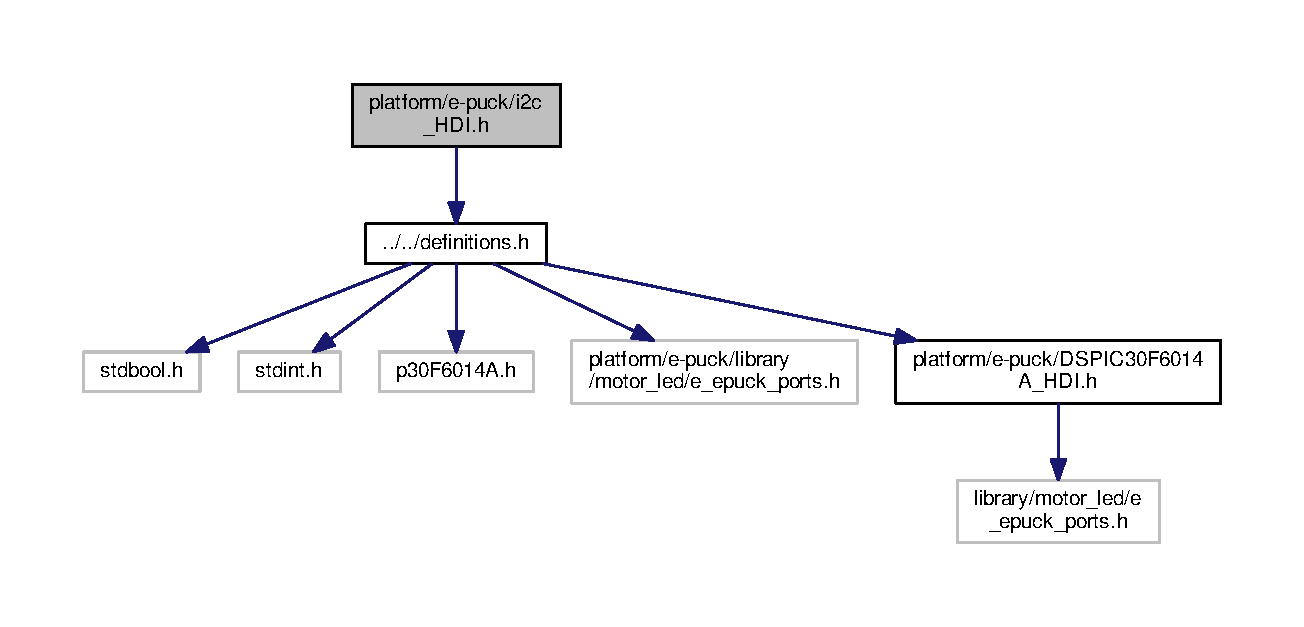
\includegraphics[width=350pt]{de/d0e/i2c__HDI_8h__incl}
\end{center}
\end{figure}
This graph shows which files directly or indirectly include this file\+:
\nopagebreak
\begin{figure}[H]
\begin{center}
\leavevmode
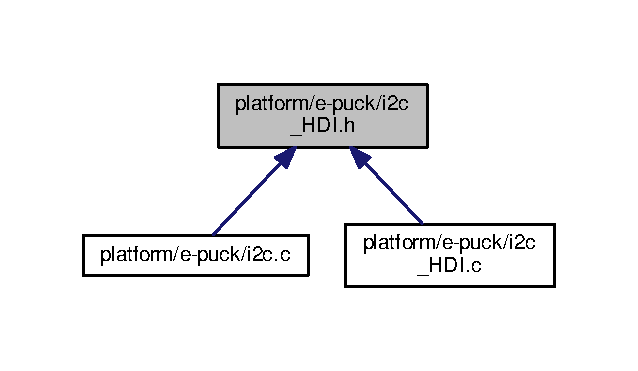
\includegraphics[width=306pt]{d8/de9/i2c__HDI_8h__dep__incl}
\end{center}
\end{figure}
\subsection*{Functions}
\begin{DoxyCompactItemize}
\item 
void \hyperlink{i2c__HDI_8h_abf50bdceb354835453ef4650790e9600}{Sys\+\_\+\+I2\+C\+\_\+\+Send\+\_\+\+Start\+\_\+\+H\+D\+I} ()
\item 
void \hyperlink{i2c__HDI_8h_aabc16d13b990930e52593cd5abb41a95}{Sys\+\_\+\+I2\+C\+\_\+\+Send\+\_\+\+Restart\+\_\+\+H\+D\+I} (void)
\item 
void \hyperlink{i2c__HDI_8h_a2d5bb88a3b7dbe61f48234700fdba614}{Sys\+\_\+\+I2\+C\+\_\+\+Send\+\_\+\+Stop\+\_\+\+H\+D\+I} (void)
\item 
void \hyperlink{i2c__HDI_8h_a2994b42ce95e10c422a7998c132c6589}{Sys\+\_\+\+I2\+C\+\_\+\+Send\+\_\+\+A\+C\+K\+\_\+\+H\+D\+I} (void)
\item 
void \hyperlink{i2c__HDI_8h_a7249b63b20eff29ce24e2e5f93a3e7ba}{Sys\+\_\+\+I2\+C\+\_\+\+Send\+\_\+\+N\+A\+C\+K\+\_\+\+H\+D\+I} (void)
\item 
void \hyperlink{i2c__HDI_8h_af1e42f570ec83376a28b6ebee1e49e44}{Sys\+\_\+\+I2\+C\+\_\+\+Start\+\_\+\+Reading\+\_\+\+H\+D\+I} (void)
\item 
char \hyperlink{i2c__HDI_8h_a25a16fa198352b2436f8db5c854585f9}{Sys\+\_\+\+I2\+C\+\_\+\+Read\+Byte\+\_\+\+H\+D\+I} (void)
\item 
void \hyperlink{i2c__HDI_8h_a5941033d2a4855c70e3321f11b846486}{Sys\+\_\+\+I2\+C\+\_\+\+Write\+Byte\+\_\+\+H\+D\+I} (\hyperlink{definitions_8h_adde6aaee8457bee49c2a92621fe22b79}{uint8} byte)
\item 
void \hyperlink{i2c__HDI_8h_aa5491239ac1f93f17b94c25867656390}{Sys\+\_\+\+Init\+\_\+\+I2\+C\+\_\+\+H\+D\+I} (void)
\item 
void \hyperlink{i2c__HDI_8h_a4c31c5ee2a65479f55423638d9dadf41}{Sys\+\_\+\+Start\+\_\+\+I2\+C\+\_\+\+H\+D\+I} (void)
\item 
void \hyperlink{i2c__HDI_8h_a2952e63416f7336bdd19cbd71bda6168}{Sys\+\_\+\+Pause\+\_\+\+I2\+C\+\_\+\+H\+D\+I} (void)
\item 
void \hyperlink{i2c__HDI_8h_a5b59f613b4a1248bc95646317cb5b7ed}{Sys\+\_\+\+Contine\+\_\+\+I2\+C\+\_\+\+H\+D\+I} (void)
\item 
void \hyperlink{i2c__HDI_8h_a2a09331981865de9c218c6cf5920ff73}{Sys\+\_\+\+Stop\+\_\+\+I2\+C\+\_\+\+H\+D\+I} (void)
\item 
void \hyperlink{i2c__HDI_8h_ad333b7abeb87e8f8c18d3dedd031ad5c}{Sys\+\_\+\+I2\+C\+\_\+\+Sent\+Bytes} (\hyperlink{definitions_8h_adde6aaee8457bee49c2a92621fe22b79}{uint8} address, \hyperlink{definitions_8h_adde6aaee8457bee49c2a92621fe22b79}{uint8} $\ast$bytes, \hyperlink{definitions_8h_a05f6b0ae8f6a6e135b0e290c25fe0e4e}{uint16} length)
\item 
void \hyperlink{i2c__HDI_8h_ab85476756c65b454eea96255916e22f9}{Sys\+\_\+\+I2\+C\+\_\+\+Read} (\hyperlink{definitions_8h_adde6aaee8457bee49c2a92621fe22b79}{uint8} address, \hyperlink{definitions_8h_adde6aaee8457bee49c2a92621fe22b79}{uint8} $\ast$intern\+\_\+address, \hyperlink{definitions_8h_a05f6b0ae8f6a6e135b0e290c25fe0e4e}{uint16} length, \hyperlink{definitions_8h_a82fa7f76266ee1d687b76a44445f21ef}{p\+Byte\+Function} bytehandler)
\end{DoxyCompactItemize}


\subsection{Detailed Description}
Hardware dependent implementations to read and write on the I2\+C interface. 

\begin{DoxyAuthor}{Author}
Stefan M. Trenkwalder \href{mailto:s.trenkwalder@openswarm.org}{\tt s.\+trenkwalder@openswarm.\+org} 
\end{DoxyAuthor}
\begin{DoxyVersion}{Version}
1.\+0
\end{DoxyVersion}
\begin{DoxyDate}{Date}
10 August 2015
\end{DoxyDate}
\begin{DoxyCopyright}{Copyright}
adapted Free\+B\+S\+D License (see \href{http://openswarm.org/license}{\tt http\+://openswarm.\+org/license}) 
\end{DoxyCopyright}


\subsection{Function Documentation}
\hypertarget{i2c__HDI_8h_a5b59f613b4a1248bc95646317cb5b7ed}{}\index{i2c\+\_\+\+H\+D\+I.\+h@{i2c\+\_\+\+H\+D\+I.\+h}!Sys\+\_\+\+Contine\+\_\+\+I2\+C\+\_\+\+H\+D\+I@{Sys\+\_\+\+Contine\+\_\+\+I2\+C\+\_\+\+H\+D\+I}}
\index{Sys\+\_\+\+Contine\+\_\+\+I2\+C\+\_\+\+H\+D\+I@{Sys\+\_\+\+Contine\+\_\+\+I2\+C\+\_\+\+H\+D\+I}!i2c\+\_\+\+H\+D\+I.\+h@{i2c\+\_\+\+H\+D\+I.\+h}}
\subsubsection[{Sys\+\_\+\+Contine\+\_\+\+I2\+C\+\_\+\+H\+D\+I}]{\setlength{\rightskip}{0pt plus 5cm}void Sys\+\_\+\+Contine\+\_\+\+I2\+C\+\_\+\+H\+D\+I (
\begin{DoxyParamCaption}
\item[{void}]{}
\end{DoxyParamCaption}
)\hspace{0.3cm}{\ttfamily [inline]}}\label{i2c__HDI_8h_a5b59f613b4a1248bc95646317cb5b7ed}
continues the I2\+C interface

This function continues the I2\+C interface. 

Definition at line 74 of file i2c\+\_\+\+H\+D\+I.\+c.

\hypertarget{i2c__HDI_8h_ab85476756c65b454eea96255916e22f9}{}\index{i2c\+\_\+\+H\+D\+I.\+h@{i2c\+\_\+\+H\+D\+I.\+h}!Sys\+\_\+\+I2\+C\+\_\+\+Read@{Sys\+\_\+\+I2\+C\+\_\+\+Read}}
\index{Sys\+\_\+\+I2\+C\+\_\+\+Read@{Sys\+\_\+\+I2\+C\+\_\+\+Read}!i2c\+\_\+\+H\+D\+I.\+h@{i2c\+\_\+\+H\+D\+I.\+h}}
\subsubsection[{Sys\+\_\+\+I2\+C\+\_\+\+Read}]{\setlength{\rightskip}{0pt plus 5cm}void Sys\+\_\+\+I2\+C\+\_\+\+Read (
\begin{DoxyParamCaption}
\item[{{\bf uint8}}]{address, }
\item[{{\bf uint8} $\ast$}]{intern\+\_\+address, }
\item[{{\bf uint16}}]{length, }
\item[{{\bf p\+Byte\+Function}}]{bytehandler}
\end{DoxyParamCaption}
)}\label{i2c__HDI_8h_ab85476756c65b454eea96255916e22f9}
reads bytes from an I2\+C device

This function first sends a reading request to the I2\+C device and, then, handles the incoming bytes with a callback function.


\begin{DoxyParams}[1]{Parameters}
\mbox{\tt in}  & {\em address} & The address of the I2\+C device that should receive the request \\
\hline
\mbox{\tt in}  & {\em intern\+\_\+address} & A pointer to the address which should be read \\
\hline
\mbox{\tt in}  & {\em length} & the number of bytes of the address \\
\hline
\mbox{\tt in}  & {\em bytehandler} & a pointer to the handler function that processes the incoming bytes. \\
\hline
\end{DoxyParams}


Definition at line 367 of file i2c.\+c.

\hypertarget{i2c__HDI_8h_a25a16fa198352b2436f8db5c854585f9}{}\index{i2c\+\_\+\+H\+D\+I.\+h@{i2c\+\_\+\+H\+D\+I.\+h}!Sys\+\_\+\+I2\+C\+\_\+\+Read\+Byte\+\_\+\+H\+D\+I@{Sys\+\_\+\+I2\+C\+\_\+\+Read\+Byte\+\_\+\+H\+D\+I}}
\index{Sys\+\_\+\+I2\+C\+\_\+\+Read\+Byte\+\_\+\+H\+D\+I@{Sys\+\_\+\+I2\+C\+\_\+\+Read\+Byte\+\_\+\+H\+D\+I}!i2c\+\_\+\+H\+D\+I.\+h@{i2c\+\_\+\+H\+D\+I.\+h}}
\subsubsection[{Sys\+\_\+\+I2\+C\+\_\+\+Read\+Byte\+\_\+\+H\+D\+I}]{\setlength{\rightskip}{0pt plus 5cm}char Sys\+\_\+\+I2\+C\+\_\+\+Read\+Byte\+\_\+\+H\+D\+I (
\begin{DoxyParamCaption}
\item[{void}]{}
\end{DoxyParamCaption}
)\hspace{0.3cm}{\ttfamily [inline]}}\label{i2c__HDI_8h_a25a16fa198352b2436f8db5c854585f9}
reads a byte via the I2\+C interface

This function reads a byte. 

Definition at line 178 of file i2c\+\_\+\+H\+D\+I.\+c.

\hypertarget{i2c__HDI_8h_a2994b42ce95e10c422a7998c132c6589}{}\index{i2c\+\_\+\+H\+D\+I.\+h@{i2c\+\_\+\+H\+D\+I.\+h}!Sys\+\_\+\+I2\+C\+\_\+\+Send\+\_\+\+A\+C\+K\+\_\+\+H\+D\+I@{Sys\+\_\+\+I2\+C\+\_\+\+Send\+\_\+\+A\+C\+K\+\_\+\+H\+D\+I}}
\index{Sys\+\_\+\+I2\+C\+\_\+\+Send\+\_\+\+A\+C\+K\+\_\+\+H\+D\+I@{Sys\+\_\+\+I2\+C\+\_\+\+Send\+\_\+\+A\+C\+K\+\_\+\+H\+D\+I}!i2c\+\_\+\+H\+D\+I.\+h@{i2c\+\_\+\+H\+D\+I.\+h}}
\subsubsection[{Sys\+\_\+\+I2\+C\+\_\+\+Send\+\_\+\+A\+C\+K\+\_\+\+H\+D\+I}]{\setlength{\rightskip}{0pt plus 5cm}void Sys\+\_\+\+I2\+C\+\_\+\+Send\+\_\+\+A\+C\+K\+\_\+\+H\+D\+I (
\begin{DoxyParamCaption}
\item[{void}]{}
\end{DoxyParamCaption}
)\hspace{0.3cm}{\ttfamily [inline]}}\label{i2c__HDI_8h_a2994b42ce95e10c422a7998c132c6589}
sends a ack bits via the I2\+C interface

This function sends a ack bits. 

Definition at line 130 of file i2c\+\_\+\+H\+D\+I.\+c.

\hypertarget{i2c__HDI_8h_a7249b63b20eff29ce24e2e5f93a3e7ba}{}\index{i2c\+\_\+\+H\+D\+I.\+h@{i2c\+\_\+\+H\+D\+I.\+h}!Sys\+\_\+\+I2\+C\+\_\+\+Send\+\_\+\+N\+A\+C\+K\+\_\+\+H\+D\+I@{Sys\+\_\+\+I2\+C\+\_\+\+Send\+\_\+\+N\+A\+C\+K\+\_\+\+H\+D\+I}}
\index{Sys\+\_\+\+I2\+C\+\_\+\+Send\+\_\+\+N\+A\+C\+K\+\_\+\+H\+D\+I@{Sys\+\_\+\+I2\+C\+\_\+\+Send\+\_\+\+N\+A\+C\+K\+\_\+\+H\+D\+I}!i2c\+\_\+\+H\+D\+I.\+h@{i2c\+\_\+\+H\+D\+I.\+h}}
\subsubsection[{Sys\+\_\+\+I2\+C\+\_\+\+Send\+\_\+\+N\+A\+C\+K\+\_\+\+H\+D\+I}]{\setlength{\rightskip}{0pt plus 5cm}void Sys\+\_\+\+I2\+C\+\_\+\+Send\+\_\+\+N\+A\+C\+K\+\_\+\+H\+D\+I (
\begin{DoxyParamCaption}
\item[{void}]{}
\end{DoxyParamCaption}
)\hspace{0.3cm}{\ttfamily [inline]}}\label{i2c__HDI_8h_a7249b63b20eff29ce24e2e5f93a3e7ba}
sends a nack bits via the I2\+C interface

This function sends a nack bits. 

Definition at line 146 of file i2c\+\_\+\+H\+D\+I.\+c.

\hypertarget{i2c__HDI_8h_aabc16d13b990930e52593cd5abb41a95}{}\index{i2c\+\_\+\+H\+D\+I.\+h@{i2c\+\_\+\+H\+D\+I.\+h}!Sys\+\_\+\+I2\+C\+\_\+\+Send\+\_\+\+Restart\+\_\+\+H\+D\+I@{Sys\+\_\+\+I2\+C\+\_\+\+Send\+\_\+\+Restart\+\_\+\+H\+D\+I}}
\index{Sys\+\_\+\+I2\+C\+\_\+\+Send\+\_\+\+Restart\+\_\+\+H\+D\+I@{Sys\+\_\+\+I2\+C\+\_\+\+Send\+\_\+\+Restart\+\_\+\+H\+D\+I}!i2c\+\_\+\+H\+D\+I.\+h@{i2c\+\_\+\+H\+D\+I.\+h}}
\subsubsection[{Sys\+\_\+\+I2\+C\+\_\+\+Send\+\_\+\+Restart\+\_\+\+H\+D\+I}]{\setlength{\rightskip}{0pt plus 5cm}void Sys\+\_\+\+I2\+C\+\_\+\+Send\+\_\+\+Restart\+\_\+\+H\+D\+I (
\begin{DoxyParamCaption}
\item[{void}]{}
\end{DoxyParamCaption}
)\hspace{0.3cm}{\ttfamily [inline]}}\label{i2c__HDI_8h_aabc16d13b990930e52593cd5abb41a95}
sends a restart bits via the I2\+C interface

This function sends a restart bits. 

Definition at line 108 of file i2c\+\_\+\+H\+D\+I.\+c.

\hypertarget{i2c__HDI_8h_abf50bdceb354835453ef4650790e9600}{}\index{i2c\+\_\+\+H\+D\+I.\+h@{i2c\+\_\+\+H\+D\+I.\+h}!Sys\+\_\+\+I2\+C\+\_\+\+Send\+\_\+\+Start\+\_\+\+H\+D\+I@{Sys\+\_\+\+I2\+C\+\_\+\+Send\+\_\+\+Start\+\_\+\+H\+D\+I}}
\index{Sys\+\_\+\+I2\+C\+\_\+\+Send\+\_\+\+Start\+\_\+\+H\+D\+I@{Sys\+\_\+\+I2\+C\+\_\+\+Send\+\_\+\+Start\+\_\+\+H\+D\+I}!i2c\+\_\+\+H\+D\+I.\+h@{i2c\+\_\+\+H\+D\+I.\+h}}
\subsubsection[{Sys\+\_\+\+I2\+C\+\_\+\+Send\+\_\+\+Start\+\_\+\+H\+D\+I}]{\setlength{\rightskip}{0pt plus 5cm}void Sys\+\_\+\+I2\+C\+\_\+\+Send\+\_\+\+Start\+\_\+\+H\+D\+I (
\begin{DoxyParamCaption}
{}
\end{DoxyParamCaption}
)\hspace{0.3cm}{\ttfamily [inline]}}\label{i2c__HDI_8h_abf50bdceb354835453ef4650790e9600}
sends a start bits via the I2\+C interface

This function sends a start bits. 

Definition at line 96 of file i2c\+\_\+\+H\+D\+I.\+c.

\hypertarget{i2c__HDI_8h_a2d5bb88a3b7dbe61f48234700fdba614}{}\index{i2c\+\_\+\+H\+D\+I.\+h@{i2c\+\_\+\+H\+D\+I.\+h}!Sys\+\_\+\+I2\+C\+\_\+\+Send\+\_\+\+Stop\+\_\+\+H\+D\+I@{Sys\+\_\+\+I2\+C\+\_\+\+Send\+\_\+\+Stop\+\_\+\+H\+D\+I}}
\index{Sys\+\_\+\+I2\+C\+\_\+\+Send\+\_\+\+Stop\+\_\+\+H\+D\+I@{Sys\+\_\+\+I2\+C\+\_\+\+Send\+\_\+\+Stop\+\_\+\+H\+D\+I}!i2c\+\_\+\+H\+D\+I.\+h@{i2c\+\_\+\+H\+D\+I.\+h}}
\subsubsection[{Sys\+\_\+\+I2\+C\+\_\+\+Send\+\_\+\+Stop\+\_\+\+H\+D\+I}]{\setlength{\rightskip}{0pt plus 5cm}void Sys\+\_\+\+I2\+C\+\_\+\+Send\+\_\+\+Stop\+\_\+\+H\+D\+I (
\begin{DoxyParamCaption}
\item[{void}]{}
\end{DoxyParamCaption}
)\hspace{0.3cm}{\ttfamily [inline]}}\label{i2c__HDI_8h_a2d5bb88a3b7dbe61f48234700fdba614}
sends a stop bits via the I2\+C interface

This function sends a stop bits. 

Definition at line 120 of file i2c\+\_\+\+H\+D\+I.\+c.

\hypertarget{i2c__HDI_8h_ad333b7abeb87e8f8c18d3dedd031ad5c}{}\index{i2c\+\_\+\+H\+D\+I.\+h@{i2c\+\_\+\+H\+D\+I.\+h}!Sys\+\_\+\+I2\+C\+\_\+\+Sent\+Bytes@{Sys\+\_\+\+I2\+C\+\_\+\+Sent\+Bytes}}
\index{Sys\+\_\+\+I2\+C\+\_\+\+Sent\+Bytes@{Sys\+\_\+\+I2\+C\+\_\+\+Sent\+Bytes}!i2c\+\_\+\+H\+D\+I.\+h@{i2c\+\_\+\+H\+D\+I.\+h}}
\subsubsection[{Sys\+\_\+\+I2\+C\+\_\+\+Sent\+Bytes}]{\setlength{\rightskip}{0pt plus 5cm}void Sys\+\_\+\+I2\+C\+\_\+\+Sent\+Bytes (
\begin{DoxyParamCaption}
\item[{{\bf uint8}}]{address, }
\item[{{\bf uint8} $\ast$}]{bytes, }
\item[{{\bf uint16}}]{length}
\end{DoxyParamCaption}
)}\label{i2c__HDI_8h_ad333b7abeb87e8f8c18d3dedd031ad5c}
adds bytes into a writing buffer

This function adds bytes into a writing buffer that are written as soon as the I2\+C is idle.

\begin{DoxyNote}{Note}
all bytes are written in sequence 
\end{DoxyNote}

\begin{DoxyParams}[1]{Parameters}
\mbox{\tt in}  & {\em address} & The address of the I2\+C device that should receive the data \\
\hline
\mbox{\tt in}  & {\em bytes} & A pointer to the data which should be sent \\
\hline
\mbox{\tt in}  & {\em length} & the number of bytes to send \\
\hline
\end{DoxyParams}


Definition at line 341 of file i2c.\+c.

\hypertarget{i2c__HDI_8h_af1e42f570ec83376a28b6ebee1e49e44}{}\index{i2c\+\_\+\+H\+D\+I.\+h@{i2c\+\_\+\+H\+D\+I.\+h}!Sys\+\_\+\+I2\+C\+\_\+\+Start\+\_\+\+Reading\+\_\+\+H\+D\+I@{Sys\+\_\+\+I2\+C\+\_\+\+Start\+\_\+\+Reading\+\_\+\+H\+D\+I}}
\index{Sys\+\_\+\+I2\+C\+\_\+\+Start\+\_\+\+Reading\+\_\+\+H\+D\+I@{Sys\+\_\+\+I2\+C\+\_\+\+Start\+\_\+\+Reading\+\_\+\+H\+D\+I}!i2c\+\_\+\+H\+D\+I.\+h@{i2c\+\_\+\+H\+D\+I.\+h}}
\subsubsection[{Sys\+\_\+\+I2\+C\+\_\+\+Start\+\_\+\+Reading\+\_\+\+H\+D\+I}]{\setlength{\rightskip}{0pt plus 5cm}void Sys\+\_\+\+I2\+C\+\_\+\+Start\+\_\+\+Reading\+\_\+\+H\+D\+I (
\begin{DoxyParamCaption}
\item[{void}]{}
\end{DoxyParamCaption}
)\hspace{0.3cm}{\ttfamily [inline]}}\label{i2c__HDI_8h_af1e42f570ec83376a28b6ebee1e49e44}
sends a reading bits via the I2\+C interface

This function sends a reading bits. 

Definition at line 162 of file i2c\+\_\+\+H\+D\+I.\+c.

\hypertarget{i2c__HDI_8h_a5941033d2a4855c70e3321f11b846486}{}\index{i2c\+\_\+\+H\+D\+I.\+h@{i2c\+\_\+\+H\+D\+I.\+h}!Sys\+\_\+\+I2\+C\+\_\+\+Write\+Byte\+\_\+\+H\+D\+I@{Sys\+\_\+\+I2\+C\+\_\+\+Write\+Byte\+\_\+\+H\+D\+I}}
\index{Sys\+\_\+\+I2\+C\+\_\+\+Write\+Byte\+\_\+\+H\+D\+I@{Sys\+\_\+\+I2\+C\+\_\+\+Write\+Byte\+\_\+\+H\+D\+I}!i2c\+\_\+\+H\+D\+I.\+h@{i2c\+\_\+\+H\+D\+I.\+h}}
\subsubsection[{Sys\+\_\+\+I2\+C\+\_\+\+Write\+Byte\+\_\+\+H\+D\+I}]{\setlength{\rightskip}{0pt plus 5cm}void Sys\+\_\+\+I2\+C\+\_\+\+Write\+Byte\+\_\+\+H\+D\+I (
\begin{DoxyParamCaption}
\item[{{\bf uint8}}]{byte}
\end{DoxyParamCaption}
)\hspace{0.3cm}{\ttfamily [inline]}}\label{i2c__HDI_8h_a5941033d2a4855c70e3321f11b846486}
writes a byte via the I2\+C interface

This function writes a byte.


\begin{DoxyParams}{Parameters}
{\em byte} & the byte that has to be written \\
\hline
\end{DoxyParams}


Definition at line 189 of file i2c\+\_\+\+H\+D\+I.\+c.

\hypertarget{i2c__HDI_8h_aa5491239ac1f93f17b94c25867656390}{}\index{i2c\+\_\+\+H\+D\+I.\+h@{i2c\+\_\+\+H\+D\+I.\+h}!Sys\+\_\+\+Init\+\_\+\+I2\+C\+\_\+\+H\+D\+I@{Sys\+\_\+\+Init\+\_\+\+I2\+C\+\_\+\+H\+D\+I}}
\index{Sys\+\_\+\+Init\+\_\+\+I2\+C\+\_\+\+H\+D\+I@{Sys\+\_\+\+Init\+\_\+\+I2\+C\+\_\+\+H\+D\+I}!i2c\+\_\+\+H\+D\+I.\+h@{i2c\+\_\+\+H\+D\+I.\+h}}
\subsubsection[{Sys\+\_\+\+Init\+\_\+\+I2\+C\+\_\+\+H\+D\+I}]{\setlength{\rightskip}{0pt plus 5cm}void Sys\+\_\+\+Init\+\_\+\+I2\+C\+\_\+\+H\+D\+I (
\begin{DoxyParamCaption}
\item[{void}]{}
\end{DoxyParamCaption}
)\hspace{0.3cm}{\ttfamily [inline]}}\label{i2c__HDI_8h_aa5491239ac1f93f17b94c25867656390}
Initialises the I2\+C interface

This function initialises the I2\+C interface. 

Definition at line 27 of file i2c\+\_\+\+H\+D\+I.\+c.

\hypertarget{i2c__HDI_8h_a2952e63416f7336bdd19cbd71bda6168}{}\index{i2c\+\_\+\+H\+D\+I.\+h@{i2c\+\_\+\+H\+D\+I.\+h}!Sys\+\_\+\+Pause\+\_\+\+I2\+C\+\_\+\+H\+D\+I@{Sys\+\_\+\+Pause\+\_\+\+I2\+C\+\_\+\+H\+D\+I}}
\index{Sys\+\_\+\+Pause\+\_\+\+I2\+C\+\_\+\+H\+D\+I@{Sys\+\_\+\+Pause\+\_\+\+I2\+C\+\_\+\+H\+D\+I}!i2c\+\_\+\+H\+D\+I.\+h@{i2c\+\_\+\+H\+D\+I.\+h}}
\subsubsection[{Sys\+\_\+\+Pause\+\_\+\+I2\+C\+\_\+\+H\+D\+I}]{\setlength{\rightskip}{0pt plus 5cm}void Sys\+\_\+\+Pause\+\_\+\+I2\+C\+\_\+\+H\+D\+I (
\begin{DoxyParamCaption}
\item[{void}]{}
\end{DoxyParamCaption}
)\hspace{0.3cm}{\ttfamily [inline]}}\label{i2c__HDI_8h_a2952e63416f7336bdd19cbd71bda6168}
pauses the I2\+C interface

This function pauses the I2\+C interface. 

Definition at line 64 of file i2c\+\_\+\+H\+D\+I.\+c.

\hypertarget{i2c__HDI_8h_a4c31c5ee2a65479f55423638d9dadf41}{}\index{i2c\+\_\+\+H\+D\+I.\+h@{i2c\+\_\+\+H\+D\+I.\+h}!Sys\+\_\+\+Start\+\_\+\+I2\+C\+\_\+\+H\+D\+I@{Sys\+\_\+\+Start\+\_\+\+I2\+C\+\_\+\+H\+D\+I}}
\index{Sys\+\_\+\+Start\+\_\+\+I2\+C\+\_\+\+H\+D\+I@{Sys\+\_\+\+Start\+\_\+\+I2\+C\+\_\+\+H\+D\+I}!i2c\+\_\+\+H\+D\+I.\+h@{i2c\+\_\+\+H\+D\+I.\+h}}
\subsubsection[{Sys\+\_\+\+Start\+\_\+\+I2\+C\+\_\+\+H\+D\+I}]{\setlength{\rightskip}{0pt plus 5cm}void Sys\+\_\+\+Start\+\_\+\+I2\+C\+\_\+\+H\+D\+I (
\begin{DoxyParamCaption}
\item[{void}]{}
\end{DoxyParamCaption}
)\hspace{0.3cm}{\ttfamily [inline]}}\label{i2c__HDI_8h_a4c31c5ee2a65479f55423638d9dadf41}
Starts the I2\+C interface

This function starts the I2\+C interface. 

Definition at line 52 of file i2c\+\_\+\+H\+D\+I.\+c.

\hypertarget{i2c__HDI_8h_a2a09331981865de9c218c6cf5920ff73}{}\index{i2c\+\_\+\+H\+D\+I.\+h@{i2c\+\_\+\+H\+D\+I.\+h}!Sys\+\_\+\+Stop\+\_\+\+I2\+C\+\_\+\+H\+D\+I@{Sys\+\_\+\+Stop\+\_\+\+I2\+C\+\_\+\+H\+D\+I}}
\index{Sys\+\_\+\+Stop\+\_\+\+I2\+C\+\_\+\+H\+D\+I@{Sys\+\_\+\+Stop\+\_\+\+I2\+C\+\_\+\+H\+D\+I}!i2c\+\_\+\+H\+D\+I.\+h@{i2c\+\_\+\+H\+D\+I.\+h}}
\subsubsection[{Sys\+\_\+\+Stop\+\_\+\+I2\+C\+\_\+\+H\+D\+I}]{\setlength{\rightskip}{0pt plus 5cm}void Sys\+\_\+\+Stop\+\_\+\+I2\+C\+\_\+\+H\+D\+I (
\begin{DoxyParamCaption}
\item[{void}]{}
\end{DoxyParamCaption}
)\hspace{0.3cm}{\ttfamily [inline]}}\label{i2c__HDI_8h_a2a09331981865de9c218c6cf5920ff73}
stops the I2\+C interface

This function stops the I2\+C interface. 

Definition at line 84 of file i2c\+\_\+\+H\+D\+I.\+c.


\hypertarget{io__HDI_8c}{}\subsection{platform/e-\/puck/io\+\_\+\+H\+D\+I.c File Reference}
\label{io__HDI_8c}\index{platform/e-\/puck/io\+\_\+\+H\+D\+I.\+c@{platform/e-\/puck/io\+\_\+\+H\+D\+I.\+c}}


Hardware dependent implementations to control the I\+O timer and to (un)register I\+O Handler.  


{\ttfamily \#include \char`\"{}io\+\_\+\+H\+D\+I.\+h\char`\"{}}\\*
{\ttfamily \#include $<$stdlib.\+h$>$}\\*
{\ttfamily \#include \char`\"{}D\+S\+P\+I\+C30\+F6014\+A\+\_\+\+H\+D\+I.\+h\char`\"{}}\\*
{\ttfamily \#include \char`\"{}../../definitions.\+h\char`\"{}}\\*
{\ttfamily \#include \char`\"{}../../interrupts.\+h\char`\"{}}\\*
{\ttfamily \#include \char`\"{}../../memory.\+h\char`\"{}}\\*
{\ttfamily \#include \char`\"{}motors.\+h\char`\"{}}\\*
Include dependency graph for io\+\_\+\+H\+D\+I.\+c\+:\nopagebreak
\begin{figure}[H]
\begin{center}
\leavevmode
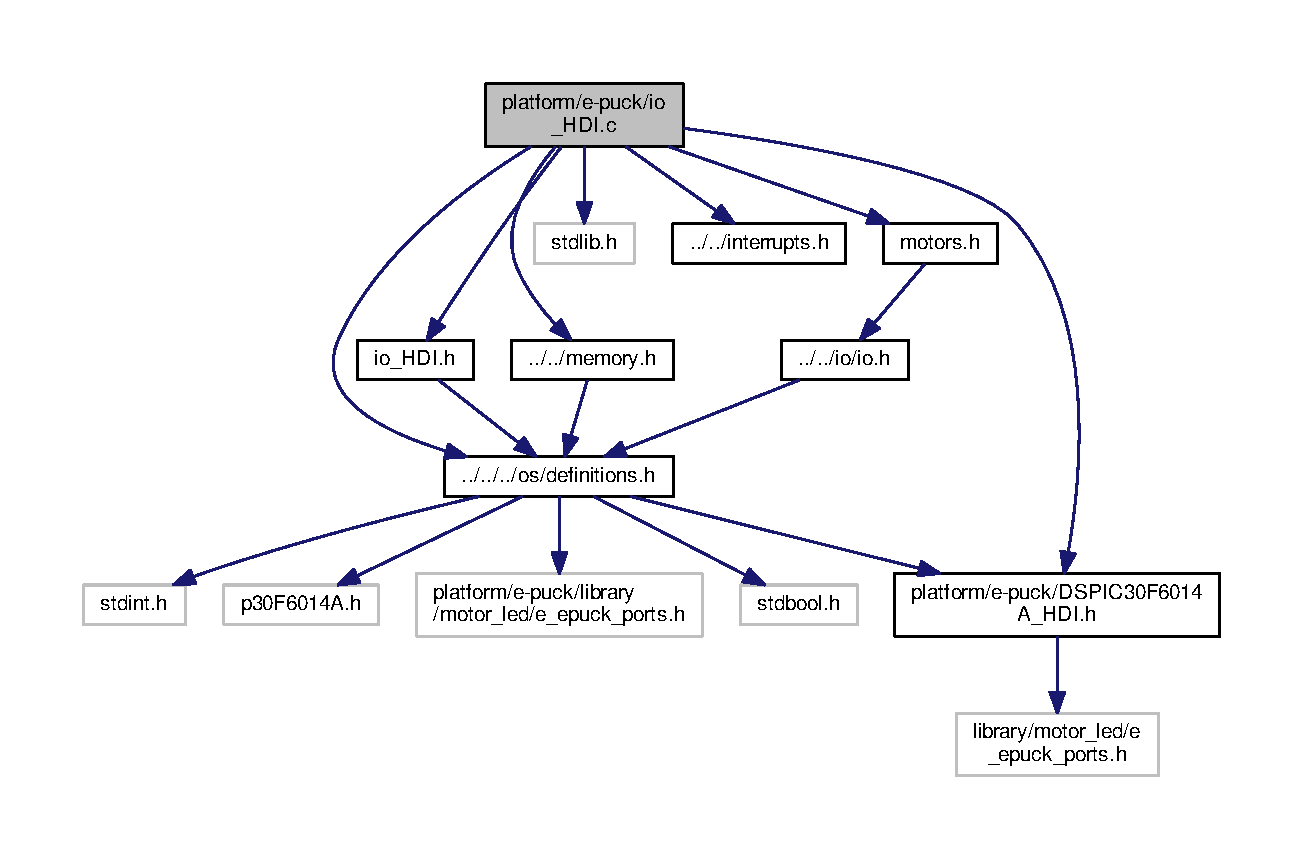
\includegraphics[width=350pt]{d0/d97/io__HDI_8c__incl}
\end{center}
\end{figure}
\subsubsection*{Functions}
\begin{DoxyCompactItemize}
\item 
void \hyperlink{io__HDI_8c_a28d9d614c7e8a65e8df36182458aeceb}{Sys\+\_\+\+Init\+\_\+\+I\+O\+Timer\+\_\+\+H\+D\+I} ()
\item 
void \hyperlink{io__HDI_8c_a2ca778d7c3009440daf51ebba3b93981}{Sys\+\_\+\+Start\+\_\+\+I\+O\+Timer\+\_\+\+H\+D\+I} ()
\item 
void \hyperlink{io__HDI_8c_a9633296082b6b8d5ef26753552bdef4c}{Sys\+\_\+\+Stop\+\_\+\+I\+O\+Timer\+\_\+\+H\+D\+I} ()
\item 
void \hyperlink{io__HDI_8c_a5a2419ba8907346f4238c00891cad779}{Sys\+\_\+\+Continue\+\_\+\+I\+O\+Timer\+\_\+\+H\+D\+I} ()
\item 
void \hyperlink{io__HDI_8c_a552c0616c1a6e9d5ad6c5b1f5f7d64f5}{Sys\+\_\+\+Reset\+\_\+\+I\+O\+Timer\+\_\+\+H\+D\+I} ()
\item 
void \hyperlink{io__HDI_8c_a226557d5e42f7e29ddaff30606138459}{\+\_\+\+\_\+attribute\+\_\+\+\_\+} ((interrupt, no\+\_\+auto\+\_\+psv))
\item 
void \hyperlink{io__HDI_8c_afcf152ee3a487aacca4dcdbd6a624411}{Sys\+\_\+\+Disable\+\_\+\+I\+O\+Timer\+Interrupt\+\_\+\+H\+D\+I} ()
\item 
void \hyperlink{io__HDI_8c_ae88f54a11740ba7a16ba5f5bab8bf42b}{Sys\+\_\+\+Enable\+\_\+\+I\+O\+Timer\+Interrupt\+\_\+\+H\+D\+I} ()
\item 
void \hyperlink{io__HDI_8c_a14c5205e2da511c4916a262b3a0f25f0}{Sys\+\_\+\+Force\+\_\+\+I\+O\+Timer\+Interrupt\+\_\+\+H\+D\+I} ()
\item 
void \hyperlink{io__HDI_8c_a396d4ef0ff2926650c4b38ebcb00c201}{Sys\+\_\+\+I\+O\+Timer\+\_\+code\+\_\+\+H\+D\+I} ()
\end{DoxyCompactItemize}
\subsubsection*{Variables}
\begin{DoxyCompactItemize}
\item 
sys\+\_\+periodical\+\_\+\+I\+O\+Handler $\ast$ \hyperlink{io__HDI_8c_a3ad4a33dee3d7041caaa39bd294644dd}{sys\+\_\+iohandlers}
\end{DoxyCompactItemize}


\subsubsection{Detailed Description}
Hardware dependent implementations to control the I\+O timer and to (un)register I\+O Handler. 

\begin{DoxyAuthor}{Author}
Stefan M. Trenkwalder \href{mailto:s.trenkwalder@openswarm.org}{\tt s.\+trenkwalder@openswarm.\+org} 
\end{DoxyAuthor}
\begin{DoxyVersion}{Version}
1.\+0
\end{DoxyVersion}
\begin{DoxyDate}{Date}
10 August 2015
\end{DoxyDate}
\begin{DoxyCopyright}{Copyright}
adapted Free\+B\+S\+D License (see \href{http://openswarm.org/license}{\tt http\+://openswarm.\+org/license}) 
\end{DoxyCopyright}


\subsubsection{Function Documentation}
\hypertarget{io__HDI_8c_a226557d5e42f7e29ddaff30606138459}{}\index{io\+\_\+\+H\+D\+I.\+c@{io\+\_\+\+H\+D\+I.\+c}!\+\_\+\+\_\+attribute\+\_\+\+\_\+@{\+\_\+\+\_\+attribute\+\_\+\+\_\+}}
\index{\+\_\+\+\_\+attribute\+\_\+\+\_\+@{\+\_\+\+\_\+attribute\+\_\+\+\_\+}!io\+\_\+\+H\+D\+I.\+c@{io\+\_\+\+H\+D\+I.\+c}}
\paragraph[{\+\_\+\+\_\+attribute\+\_\+\+\_\+}]{\setlength{\rightskip}{0pt plus 5cm}void \+\_\+\+\_\+attribute\+\_\+\+\_\+ (
\begin{DoxyParamCaption}
\item[{(interrupt, no\+\_\+auto\+\_\+psv)}]{}
\end{DoxyParamCaption}
)}\label{io__HDI_8c_a226557d5e42f7e29ddaff30606138459}
This Function starts the task-\/scheduling algorithm

Interrupt Service Routine for the Timer1 (alternate) starts the task-\/scheduling algorithm

Address error trap.

This function is called when an address error occurs. That means that a call address of a function or in the stack addresses an area outside the memory. Similarly, if a pointer points to memory outside the range, this trap happens.

Stack error trap.

This function is called when an stack error occurs. That means that the stack pointer, stack pointer limit, or frame pointer are pointing outside their range.

Math error trap.

This function is called when an math error occurs. That means an illegal math operation was performed (such as division by 0 or Na\+N).

Alternative Oscillator fail trap.

This function is called when an oscillator fail occurs. This should never happen.

Alternative address error trap.

This function is called when an address error occurs. That means that a call address of a function or in the stack addresses an area outside the memory. Similarly, if a pointer points to memory outside the range, this trap happens.

Alternative stack error trap.

This function is called when an stack error occurs. That means that the stack pointer, stack pointer limit, or frame pointer are pointing outside their range.

Alternative math error trap.

This function is called when an math error occurs. That means an illegal math operation was performed (such as division by 0 or Na\+N).

Default interrupt service routine.

This function is called when no other interrupt routine is specified. 

Definition at line 103 of file io\+\_\+\+H\+D\+I.\+c.

\hypertarget{io__HDI_8c_a5a2419ba8907346f4238c00891cad779}{}\index{io\+\_\+\+H\+D\+I.\+c@{io\+\_\+\+H\+D\+I.\+c}!Sys\+\_\+\+Continue\+\_\+\+I\+O\+Timer\+\_\+\+H\+D\+I@{Sys\+\_\+\+Continue\+\_\+\+I\+O\+Timer\+\_\+\+H\+D\+I}}
\index{Sys\+\_\+\+Continue\+\_\+\+I\+O\+Timer\+\_\+\+H\+D\+I@{Sys\+\_\+\+Continue\+\_\+\+I\+O\+Timer\+\_\+\+H\+D\+I}!io\+\_\+\+H\+D\+I.\+c@{io\+\_\+\+H\+D\+I.\+c}}
\paragraph[{Sys\+\_\+\+Continue\+\_\+\+I\+O\+Timer\+\_\+\+H\+D\+I}]{\setlength{\rightskip}{0pt plus 5cm}void Sys\+\_\+\+Continue\+\_\+\+I\+O\+Timer\+\_\+\+H\+D\+I (
\begin{DoxyParamCaption}
\item[{void}]{}
\end{DoxyParamCaption}
)\hspace{0.3cm}{\ttfamily [inline]}}\label{io__HDI_8c_a5a2419ba8907346f4238c00891cad779}
This function continues the I/\+O Timer. 

Definition at line 81 of file io\+\_\+\+H\+D\+I.\+c.

\hypertarget{io__HDI_8c_afcf152ee3a487aacca4dcdbd6a624411}{}\index{io\+\_\+\+H\+D\+I.\+c@{io\+\_\+\+H\+D\+I.\+c}!Sys\+\_\+\+Disable\+\_\+\+I\+O\+Timer\+Interrupt\+\_\+\+H\+D\+I@{Sys\+\_\+\+Disable\+\_\+\+I\+O\+Timer\+Interrupt\+\_\+\+H\+D\+I}}
\index{Sys\+\_\+\+Disable\+\_\+\+I\+O\+Timer\+Interrupt\+\_\+\+H\+D\+I@{Sys\+\_\+\+Disable\+\_\+\+I\+O\+Timer\+Interrupt\+\_\+\+H\+D\+I}!io\+\_\+\+H\+D\+I.\+c@{io\+\_\+\+H\+D\+I.\+c}}
\paragraph[{Sys\+\_\+\+Disable\+\_\+\+I\+O\+Timer\+Interrupt\+\_\+\+H\+D\+I}]{\setlength{\rightskip}{0pt plus 5cm}void Sys\+\_\+\+Disable\+\_\+\+I\+O\+Timer\+Interrupt\+\_\+\+H\+D\+I (
\begin{DoxyParamCaption}
\item[{void}]{}
\end{DoxyParamCaption}
)\hspace{0.3cm}{\ttfamily [inline]}}\label{io__HDI_8c_afcf152ee3a487aacca4dcdbd6a624411}
Disables the Timer1 interrupt and sets the interrupt flag to 0 

Definition at line 122 of file io\+\_\+\+H\+D\+I.\+c.

\hypertarget{io__HDI_8c_ae88f54a11740ba7a16ba5f5bab8bf42b}{}\index{io\+\_\+\+H\+D\+I.\+c@{io\+\_\+\+H\+D\+I.\+c}!Sys\+\_\+\+Enable\+\_\+\+I\+O\+Timer\+Interrupt\+\_\+\+H\+D\+I@{Sys\+\_\+\+Enable\+\_\+\+I\+O\+Timer\+Interrupt\+\_\+\+H\+D\+I}}
\index{Sys\+\_\+\+Enable\+\_\+\+I\+O\+Timer\+Interrupt\+\_\+\+H\+D\+I@{Sys\+\_\+\+Enable\+\_\+\+I\+O\+Timer\+Interrupt\+\_\+\+H\+D\+I}!io\+\_\+\+H\+D\+I.\+c@{io\+\_\+\+H\+D\+I.\+c}}
\paragraph[{Sys\+\_\+\+Enable\+\_\+\+I\+O\+Timer\+Interrupt\+\_\+\+H\+D\+I}]{\setlength{\rightskip}{0pt plus 5cm}void Sys\+\_\+\+Enable\+\_\+\+I\+O\+Timer\+Interrupt\+\_\+\+H\+D\+I (
\begin{DoxyParamCaption}
\item[{void}]{}
\end{DoxyParamCaption}
)\hspace{0.3cm}{\ttfamily [inline]}}\label{io__HDI_8c_ae88f54a11740ba7a16ba5f5bab8bf42b}
Enables the Timer1 interrupt and leaves the interrupt flag to its value. If the flag was set, the Timer1 interrupt will be emitted after executing this function. 

Definition at line 132 of file io\+\_\+\+H\+D\+I.\+c.

\hypertarget{io__HDI_8c_a14c5205e2da511c4916a262b3a0f25f0}{}\index{io\+\_\+\+H\+D\+I.\+c@{io\+\_\+\+H\+D\+I.\+c}!Sys\+\_\+\+Force\+\_\+\+I\+O\+Timer\+Interrupt\+\_\+\+H\+D\+I@{Sys\+\_\+\+Force\+\_\+\+I\+O\+Timer\+Interrupt\+\_\+\+H\+D\+I}}
\index{Sys\+\_\+\+Force\+\_\+\+I\+O\+Timer\+Interrupt\+\_\+\+H\+D\+I@{Sys\+\_\+\+Force\+\_\+\+I\+O\+Timer\+Interrupt\+\_\+\+H\+D\+I}!io\+\_\+\+H\+D\+I.\+c@{io\+\_\+\+H\+D\+I.\+c}}
\paragraph[{Sys\+\_\+\+Force\+\_\+\+I\+O\+Timer\+Interrupt\+\_\+\+H\+D\+I}]{\setlength{\rightskip}{0pt plus 5cm}void Sys\+\_\+\+Force\+\_\+\+I\+O\+Timer\+Interrupt\+\_\+\+H\+D\+I (
\begin{DoxyParamCaption}
\item[{void}]{}
\end{DoxyParamCaption}
)\hspace{0.3cm}{\ttfamily [inline]}}\label{io__HDI_8c_a14c5205e2da511c4916a262b3a0f25f0}
forces the Timer1 interrupt to occur. 

Definition at line 140 of file io\+\_\+\+H\+D\+I.\+c.

\hypertarget{io__HDI_8c_a28d9d614c7e8a65e8df36182458aeceb}{}\index{io\+\_\+\+H\+D\+I.\+c@{io\+\_\+\+H\+D\+I.\+c}!Sys\+\_\+\+Init\+\_\+\+I\+O\+Timer\+\_\+\+H\+D\+I@{Sys\+\_\+\+Init\+\_\+\+I\+O\+Timer\+\_\+\+H\+D\+I}}
\index{Sys\+\_\+\+Init\+\_\+\+I\+O\+Timer\+\_\+\+H\+D\+I@{Sys\+\_\+\+Init\+\_\+\+I\+O\+Timer\+\_\+\+H\+D\+I}!io\+\_\+\+H\+D\+I.\+c@{io\+\_\+\+H\+D\+I.\+c}}
\paragraph[{Sys\+\_\+\+Init\+\_\+\+I\+O\+Timer\+\_\+\+H\+D\+I}]{\setlength{\rightskip}{0pt plus 5cm}void Sys\+\_\+\+Init\+\_\+\+I\+O\+Timer\+\_\+\+H\+D\+I (
\begin{DoxyParamCaption}
{}
\end{DoxyParamCaption}
)\hspace{0.3cm}{\ttfamily [inline]}}\label{io__HDI_8c_a28d9d614c7e8a65e8df36182458aeceb}
This function initialises the I/\+O Timer. 

Definition at line 33 of file io\+\_\+\+H\+D\+I.\+c.

\hypertarget{io__HDI_8c_a396d4ef0ff2926650c4b38ebcb00c201}{}\index{io\+\_\+\+H\+D\+I.\+c@{io\+\_\+\+H\+D\+I.\+c}!Sys\+\_\+\+I\+O\+Timer\+\_\+code\+\_\+\+H\+D\+I@{Sys\+\_\+\+I\+O\+Timer\+\_\+code\+\_\+\+H\+D\+I}}
\index{Sys\+\_\+\+I\+O\+Timer\+\_\+code\+\_\+\+H\+D\+I@{Sys\+\_\+\+I\+O\+Timer\+\_\+code\+\_\+\+H\+D\+I}!io\+\_\+\+H\+D\+I.\+c@{io\+\_\+\+H\+D\+I.\+c}}
\paragraph[{Sys\+\_\+\+I\+O\+Timer\+\_\+code\+\_\+\+H\+D\+I}]{\setlength{\rightskip}{0pt plus 5cm}void Sys\+\_\+\+I\+O\+Timer\+\_\+code\+\_\+\+H\+D\+I (
\begin{DoxyParamCaption}
{}
\end{DoxyParamCaption}
)\hspace{0.3cm}{\ttfamily [inline]}}\label{io__HDI_8c_a396d4ef0ff2926650c4b38ebcb00c201}
This function is executed every time the I/\+O timer is active and executes all I/\+O handlers 

Definition at line 149 of file io\+\_\+\+H\+D\+I.\+c.

\hypertarget{io__HDI_8c_a552c0616c1a6e9d5ad6c5b1f5f7d64f5}{}\index{io\+\_\+\+H\+D\+I.\+c@{io\+\_\+\+H\+D\+I.\+c}!Sys\+\_\+\+Reset\+\_\+\+I\+O\+Timer\+\_\+\+H\+D\+I@{Sys\+\_\+\+Reset\+\_\+\+I\+O\+Timer\+\_\+\+H\+D\+I}}
\index{Sys\+\_\+\+Reset\+\_\+\+I\+O\+Timer\+\_\+\+H\+D\+I@{Sys\+\_\+\+Reset\+\_\+\+I\+O\+Timer\+\_\+\+H\+D\+I}!io\+\_\+\+H\+D\+I.\+c@{io\+\_\+\+H\+D\+I.\+c}}
\paragraph[{Sys\+\_\+\+Reset\+\_\+\+I\+O\+Timer\+\_\+\+H\+D\+I}]{\setlength{\rightskip}{0pt plus 5cm}void Sys\+\_\+\+Reset\+\_\+\+I\+O\+Timer\+\_\+\+H\+D\+I (
\begin{DoxyParamCaption}
\item[{void}]{}
\end{DoxyParamCaption}
)\hspace{0.3cm}{\ttfamily [inline]}}\label{io__HDI_8c_a552c0616c1a6e9d5ad6c5b1f5f7d64f5}
This function resets the I/\+O Timer. 

Definition at line 93 of file io\+\_\+\+H\+D\+I.\+c.

\hypertarget{io__HDI_8c_a2ca778d7c3009440daf51ebba3b93981}{}\index{io\+\_\+\+H\+D\+I.\+c@{io\+\_\+\+H\+D\+I.\+c}!Sys\+\_\+\+Start\+\_\+\+I\+O\+Timer\+\_\+\+H\+D\+I@{Sys\+\_\+\+Start\+\_\+\+I\+O\+Timer\+\_\+\+H\+D\+I}}
\index{Sys\+\_\+\+Start\+\_\+\+I\+O\+Timer\+\_\+\+H\+D\+I@{Sys\+\_\+\+Start\+\_\+\+I\+O\+Timer\+\_\+\+H\+D\+I}!io\+\_\+\+H\+D\+I.\+c@{io\+\_\+\+H\+D\+I.\+c}}
\paragraph[{Sys\+\_\+\+Start\+\_\+\+I\+O\+Timer\+\_\+\+H\+D\+I}]{\setlength{\rightskip}{0pt plus 5cm}void Sys\+\_\+\+Start\+\_\+\+I\+O\+Timer\+\_\+\+H\+D\+I (
\begin{DoxyParamCaption}
{}
\end{DoxyParamCaption}
)\hspace{0.3cm}{\ttfamily [inline]}}\label{io__HDI_8c_a2ca778d7c3009440daf51ebba3b93981}
This function starts the I/\+O Timer. $<$ interrupt priority for the I/\+O timer interrupt 

Definition at line 57 of file io\+\_\+\+H\+D\+I.\+c.

\hypertarget{io__HDI_8c_a9633296082b6b8d5ef26753552bdef4c}{}\index{io\+\_\+\+H\+D\+I.\+c@{io\+\_\+\+H\+D\+I.\+c}!Sys\+\_\+\+Stop\+\_\+\+I\+O\+Timer\+\_\+\+H\+D\+I@{Sys\+\_\+\+Stop\+\_\+\+I\+O\+Timer\+\_\+\+H\+D\+I}}
\index{Sys\+\_\+\+Stop\+\_\+\+I\+O\+Timer\+\_\+\+H\+D\+I@{Sys\+\_\+\+Stop\+\_\+\+I\+O\+Timer\+\_\+\+H\+D\+I}!io\+\_\+\+H\+D\+I.\+c@{io\+\_\+\+H\+D\+I.\+c}}
\paragraph[{Sys\+\_\+\+Stop\+\_\+\+I\+O\+Timer\+\_\+\+H\+D\+I}]{\setlength{\rightskip}{0pt plus 5cm}void Sys\+\_\+\+Stop\+\_\+\+I\+O\+Timer\+\_\+\+H\+D\+I (
\begin{DoxyParamCaption}
\item[{void}]{}
\end{DoxyParamCaption}
)\hspace{0.3cm}{\ttfamily [inline]}}\label{io__HDI_8c_a9633296082b6b8d5ef26753552bdef4c}
This function stops the I/\+O Timer. 

Definition at line 69 of file io\+\_\+\+H\+D\+I.\+c.



\subsubsection{Variable Documentation}
\hypertarget{io__HDI_8c_a3ad4a33dee3d7041caaa39bd294644dd}{}\index{io\+\_\+\+H\+D\+I.\+c@{io\+\_\+\+H\+D\+I.\+c}!sys\+\_\+iohandlers@{sys\+\_\+iohandlers}}
\index{sys\+\_\+iohandlers@{sys\+\_\+iohandlers}!io\+\_\+\+H\+D\+I.\+c@{io\+\_\+\+H\+D\+I.\+c}}
\paragraph[{sys\+\_\+iohandlers}]{\setlength{\rightskip}{0pt plus 5cm}sys\+\_\+periodical\+\_\+\+I\+O\+Handler$\ast$ sys\+\_\+iohandlers}\label{io__HDI_8c_a3ad4a33dee3d7041caaa39bd294644dd}
List of I/\+O handlers 

Definition at line 25 of file io\+\_\+\+H\+D\+I.\+c.


\hypertarget{io__HDI_8h}{}\section{platform/e-\/puck/io\+\_\+\+H\+D\+I.h File Reference}
\label{io__HDI_8h}\index{platform/e-\/puck/io\+\_\+\+H\+D\+I.\+h@{platform/e-\/puck/io\+\_\+\+H\+D\+I.\+h}}


Hardware dependent implementations to start and stop the I/\+O timer. This timer executes I\+O functions periodically.  


{\ttfamily \#include \char`\"{}../../../os/definitions.\+h\char`\"{}}\\*
Include dependency graph for io\+\_\+\+H\+D\+I.\+h\+:\nopagebreak
\begin{figure}[H]
\begin{center}
\leavevmode
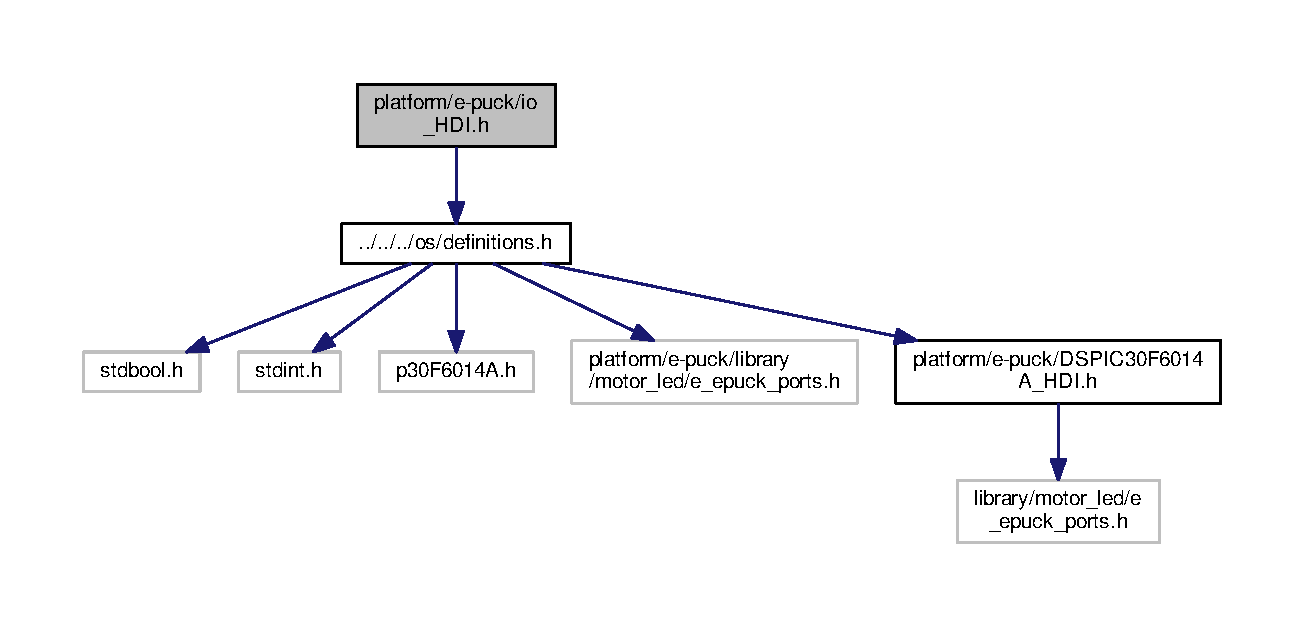
\includegraphics[width=350pt]{dd/d6f/io__HDI_8h__incl}
\end{center}
\end{figure}
This graph shows which files directly or indirectly include this file\+:\nopagebreak
\begin{figure}[H]
\begin{center}
\leavevmode
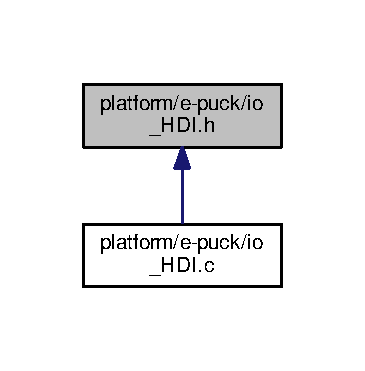
\includegraphics[width=175pt]{da/d19/io__HDI_8h__dep__incl}
\end{center}
\end{figure}
\subsection*{Data Structures}
\begin{DoxyCompactItemize}
\item 
struct \hyperlink{structsys__periodical__IOHandler__s}{sys\+\_\+periodical\+\_\+\+I\+O\+Handler\+\_\+s}
\end{DoxyCompactItemize}
\subsection*{Macros}
\begin{DoxyCompactItemize}
\item 
\#define \hyperlink{io__HDI_8h_a56fda60ac404cbe74f78b91bcf40b856}{S\+T\+E\+P\+S\+\_\+\+P\+E\+R\+\_\+\+S\+E\+C\+O\+N\+D}~10000
\item 
\#define \hyperlink{io__HDI_8h_a7defcba4392b3bfd9ade0e27f5c5c173}{S\+T\+E\+P\+S\+\_\+\+P\+E\+R\+\_\+\+M\+I\+L\+I\+S\+E\+C\+O\+N\+D}~10
\end{DoxyCompactItemize}
\subsection*{Typedefs}
\begin{DoxyCompactItemize}
\item 
typedef struct \hyperlink{structsys__periodical__IOHandler__s}{sys\+\_\+periodical\+\_\+\+I\+O\+Handler\+\_\+s} \hyperlink{io__HDI_8h_ad7821201f73ad9a8f829d1883ef2346d}{sys\+\_\+periodical\+\_\+\+I\+O\+Handler}
\item 
typedef struct \hyperlink{structsys__periodical__IOHandler__s}{sys\+\_\+periodical\+\_\+\+I\+O\+Handler\+\_\+s} \hyperlink{io__HDI_8h_a2c21c7610a28b36d1a142eecf10f78a5}{sys\+\_\+p\+I\+O\+Handler}
\end{DoxyCompactItemize}
\subsection*{Functions}
\begin{DoxyCompactItemize}
\item 
void \hyperlink{io__HDI_8h_a28d9d614c7e8a65e8df36182458aeceb}{Sys\+\_\+\+Init\+\_\+\+I\+O\+Timer\+\_\+\+H\+D\+I} ()
\item 
void \hyperlink{io__HDI_8h_a2ca778d7c3009440daf51ebba3b93981}{Sys\+\_\+\+Start\+\_\+\+I\+O\+Timer\+\_\+\+H\+D\+I} ()
\item 
void \hyperlink{io__HDI_8h_a396d4ef0ff2926650c4b38ebcb00c201}{Sys\+\_\+\+I\+O\+Timer\+\_\+code\+\_\+\+H\+D\+I} ()
\item 
void \hyperlink{io__HDI_8h_af127738e18e8d65b197f10459ee6d759}{Sys\+\_\+\+Stop\+\_\+\+I\+O\+Timer\+\_\+\+H\+D\+I} (void)
\item 
void \hyperlink{io__HDI_8h_af772d5039f6c3e70af18551080e75add}{Sys\+\_\+\+Continue\+\_\+\+I\+O\+Timer\+\_\+\+H\+D\+I} (void)
\item 
void \hyperlink{io__HDI_8h_a3240e6a33b3b9c0669b6756b9586535f}{Sys\+\_\+\+Reset\+\_\+\+I\+O\+Timer\+\_\+\+H\+D\+I} (void)
\item 
void \hyperlink{io__HDI_8h_a70209100a4406009be4bbf3a17257556}{Sys\+\_\+\+Disable\+\_\+\+I\+O\+Timer\+Interrupt\+\_\+\+H\+D\+I} (void)
\item 
void \hyperlink{io__HDI_8h_a8ab90b7c30fe74694b4031fb80e7087d}{Sys\+\_\+\+Enable\+\_\+\+I\+O\+Timer\+Interrupt\+\_\+\+H\+D\+I} (void)
\item 
void \hyperlink{io__HDI_8h_aa1462398cf5f47c6c48d8c3ee7aac193}{Sys\+\_\+\+Force\+\_\+\+I\+O\+Timer\+Interrupt\+\_\+\+H\+D\+I} (void)
\end{DoxyCompactItemize}
\subsection*{Variables}
\begin{DoxyCompactItemize}
\item 
\hyperlink{io__HDI_8h_ad7821201f73ad9a8f829d1883ef2346d}{sys\+\_\+periodical\+\_\+\+I\+O\+Handler} $\ast$ \hyperlink{io__HDI_8h_a3ad4a33dee3d7041caaa39bd294644dd}{sys\+\_\+iohandlers}
\end{DoxyCompactItemize}


\subsection{Detailed Description}
Hardware dependent implementations to start and stop the I/\+O timer. This timer executes I\+O functions periodically. 

\begin{DoxyAuthor}{Author}
Stefan M. Trenkwalder \href{mailto:s.trenkwalder@openswarm.org}{\tt s.\+trenkwalder@openswarm.\+org} 
\end{DoxyAuthor}
\begin{DoxyVersion}{Version}
1.\+0
\end{DoxyVersion}
\begin{DoxyDate}{Date}
10 August 2015
\end{DoxyDate}
\begin{DoxyCopyright}{Copyright}
adapted Free\+B\+S\+D License (see \href{http://openswarm.org/license}{\tt http\+://openswarm.\+org/license}) 
\end{DoxyCopyright}


\subsection{Macro Definition Documentation}
\hypertarget{io__HDI_8h_a7defcba4392b3bfd9ade0e27f5c5c173}{}\index{io\+\_\+\+H\+D\+I.\+h@{io\+\_\+\+H\+D\+I.\+h}!S\+T\+E\+P\+S\+\_\+\+P\+E\+R\+\_\+\+M\+I\+L\+I\+S\+E\+C\+O\+N\+D@{S\+T\+E\+P\+S\+\_\+\+P\+E\+R\+\_\+\+M\+I\+L\+I\+S\+E\+C\+O\+N\+D}}
\index{S\+T\+E\+P\+S\+\_\+\+P\+E\+R\+\_\+\+M\+I\+L\+I\+S\+E\+C\+O\+N\+D@{S\+T\+E\+P\+S\+\_\+\+P\+E\+R\+\_\+\+M\+I\+L\+I\+S\+E\+C\+O\+N\+D}!io\+\_\+\+H\+D\+I.\+h@{io\+\_\+\+H\+D\+I.\+h}}
\subsubsection[{S\+T\+E\+P\+S\+\_\+\+P\+E\+R\+\_\+\+M\+I\+L\+I\+S\+E\+C\+O\+N\+D}]{\setlength{\rightskip}{0pt plus 5cm}\#define S\+T\+E\+P\+S\+\_\+\+P\+E\+R\+\_\+\+M\+I\+L\+I\+S\+E\+C\+O\+N\+D~10}\label{io__HDI_8h_a7defcba4392b3bfd9ade0e27f5c5c173}


Definition at line 26 of file io\+\_\+\+H\+D\+I.\+h.

\hypertarget{io__HDI_8h_a56fda60ac404cbe74f78b91bcf40b856}{}\index{io\+\_\+\+H\+D\+I.\+h@{io\+\_\+\+H\+D\+I.\+h}!S\+T\+E\+P\+S\+\_\+\+P\+E\+R\+\_\+\+S\+E\+C\+O\+N\+D@{S\+T\+E\+P\+S\+\_\+\+P\+E\+R\+\_\+\+S\+E\+C\+O\+N\+D}}
\index{S\+T\+E\+P\+S\+\_\+\+P\+E\+R\+\_\+\+S\+E\+C\+O\+N\+D@{S\+T\+E\+P\+S\+\_\+\+P\+E\+R\+\_\+\+S\+E\+C\+O\+N\+D}!io\+\_\+\+H\+D\+I.\+h@{io\+\_\+\+H\+D\+I.\+h}}
\subsubsection[{S\+T\+E\+P\+S\+\_\+\+P\+E\+R\+\_\+\+S\+E\+C\+O\+N\+D}]{\setlength{\rightskip}{0pt plus 5cm}\#define S\+T\+E\+P\+S\+\_\+\+P\+E\+R\+\_\+\+S\+E\+C\+O\+N\+D~10000}\label{io__HDI_8h_a56fda60ac404cbe74f78b91bcf40b856}


Definition at line 25 of file io\+\_\+\+H\+D\+I.\+h.



\subsection{Typedef Documentation}
\hypertarget{io__HDI_8h_ad7821201f73ad9a8f829d1883ef2346d}{}\index{io\+\_\+\+H\+D\+I.\+h@{io\+\_\+\+H\+D\+I.\+h}!sys\+\_\+periodical\+\_\+\+I\+O\+Handler@{sys\+\_\+periodical\+\_\+\+I\+O\+Handler}}
\index{sys\+\_\+periodical\+\_\+\+I\+O\+Handler@{sys\+\_\+periodical\+\_\+\+I\+O\+Handler}!io\+\_\+\+H\+D\+I.\+h@{io\+\_\+\+H\+D\+I.\+h}}
\subsubsection[{sys\+\_\+periodical\+\_\+\+I\+O\+Handler}]{\setlength{\rightskip}{0pt plus 5cm}typedef struct {\bf sys\+\_\+periodical\+\_\+\+I\+O\+Handler\+\_\+s}  {\bf sys\+\_\+periodical\+\_\+\+I\+O\+Handler}}\label{io__HDI_8h_ad7821201f73ad9a8f829d1883ef2346d}
\hypertarget{io__HDI_8h_a2c21c7610a28b36d1a142eecf10f78a5}{}\index{io\+\_\+\+H\+D\+I.\+h@{io\+\_\+\+H\+D\+I.\+h}!sys\+\_\+p\+I\+O\+Handler@{sys\+\_\+p\+I\+O\+Handler}}
\index{sys\+\_\+p\+I\+O\+Handler@{sys\+\_\+p\+I\+O\+Handler}!io\+\_\+\+H\+D\+I.\+h@{io\+\_\+\+H\+D\+I.\+h}}
\subsubsection[{sys\+\_\+p\+I\+O\+Handler}]{\setlength{\rightskip}{0pt plus 5cm}typedef struct {\bf sys\+\_\+periodical\+\_\+\+I\+O\+Handler\+\_\+s}  {\bf sys\+\_\+p\+I\+O\+Handler}}\label{io__HDI_8h_a2c21c7610a28b36d1a142eecf10f78a5}


\subsection{Function Documentation}
\hypertarget{io__HDI_8h_af772d5039f6c3e70af18551080e75add}{}\index{io\+\_\+\+H\+D\+I.\+h@{io\+\_\+\+H\+D\+I.\+h}!Sys\+\_\+\+Continue\+\_\+\+I\+O\+Timer\+\_\+\+H\+D\+I@{Sys\+\_\+\+Continue\+\_\+\+I\+O\+Timer\+\_\+\+H\+D\+I}}
\index{Sys\+\_\+\+Continue\+\_\+\+I\+O\+Timer\+\_\+\+H\+D\+I@{Sys\+\_\+\+Continue\+\_\+\+I\+O\+Timer\+\_\+\+H\+D\+I}!io\+\_\+\+H\+D\+I.\+h@{io\+\_\+\+H\+D\+I.\+h}}
\subsubsection[{Sys\+\_\+\+Continue\+\_\+\+I\+O\+Timer\+\_\+\+H\+D\+I}]{\setlength{\rightskip}{0pt plus 5cm}void Sys\+\_\+\+Continue\+\_\+\+I\+O\+Timer\+\_\+\+H\+D\+I (
\begin{DoxyParamCaption}
\item[{void}]{}
\end{DoxyParamCaption}
)\hspace{0.3cm}{\ttfamily [inline]}}\label{io__HDI_8h_af772d5039f6c3e70af18551080e75add}
continues the I/\+O Timer

This function continues the I/\+O Timer. 

Definition at line 86 of file io\+\_\+\+H\+D\+I.\+c.

\hypertarget{io__HDI_8h_a70209100a4406009be4bbf3a17257556}{}\index{io\+\_\+\+H\+D\+I.\+h@{io\+\_\+\+H\+D\+I.\+h}!Sys\+\_\+\+Disable\+\_\+\+I\+O\+Timer\+Interrupt\+\_\+\+H\+D\+I@{Sys\+\_\+\+Disable\+\_\+\+I\+O\+Timer\+Interrupt\+\_\+\+H\+D\+I}}
\index{Sys\+\_\+\+Disable\+\_\+\+I\+O\+Timer\+Interrupt\+\_\+\+H\+D\+I@{Sys\+\_\+\+Disable\+\_\+\+I\+O\+Timer\+Interrupt\+\_\+\+H\+D\+I}!io\+\_\+\+H\+D\+I.\+h@{io\+\_\+\+H\+D\+I.\+h}}
\subsubsection[{Sys\+\_\+\+Disable\+\_\+\+I\+O\+Timer\+Interrupt\+\_\+\+H\+D\+I}]{\setlength{\rightskip}{0pt plus 5cm}void Sys\+\_\+\+Disable\+\_\+\+I\+O\+Timer\+Interrupt\+\_\+\+H\+D\+I (
\begin{DoxyParamCaption}
\item[{void}]{}
\end{DoxyParamCaption}
)\hspace{0.3cm}{\ttfamily [inline]}}\label{io__HDI_8h_a70209100a4406009be4bbf3a17257556}
Disables the Timer1 interrupt

Disables the Timer1 interrupt and sets the interrupt flag to 0 

Definition at line 132 of file io\+\_\+\+H\+D\+I.\+c.

\hypertarget{io__HDI_8h_a8ab90b7c30fe74694b4031fb80e7087d}{}\index{io\+\_\+\+H\+D\+I.\+h@{io\+\_\+\+H\+D\+I.\+h}!Sys\+\_\+\+Enable\+\_\+\+I\+O\+Timer\+Interrupt\+\_\+\+H\+D\+I@{Sys\+\_\+\+Enable\+\_\+\+I\+O\+Timer\+Interrupt\+\_\+\+H\+D\+I}}
\index{Sys\+\_\+\+Enable\+\_\+\+I\+O\+Timer\+Interrupt\+\_\+\+H\+D\+I@{Sys\+\_\+\+Enable\+\_\+\+I\+O\+Timer\+Interrupt\+\_\+\+H\+D\+I}!io\+\_\+\+H\+D\+I.\+h@{io\+\_\+\+H\+D\+I.\+h}}
\subsubsection[{Sys\+\_\+\+Enable\+\_\+\+I\+O\+Timer\+Interrupt\+\_\+\+H\+D\+I}]{\setlength{\rightskip}{0pt plus 5cm}void Sys\+\_\+\+Enable\+\_\+\+I\+O\+Timer\+Interrupt\+\_\+\+H\+D\+I (
\begin{DoxyParamCaption}
\item[{void}]{}
\end{DoxyParamCaption}
)\hspace{0.3cm}{\ttfamily [inline]}}\label{io__HDI_8h_a8ab90b7c30fe74694b4031fb80e7087d}
Enables the Timer1 interrupt

Enables the Timer1 interrupt and leaves the interrupt flag to its value. If the flag was set, the Timer1 interrupt will be emitted after executing this function. 

Definition at line 143 of file io\+\_\+\+H\+D\+I.\+c.

\hypertarget{io__HDI_8h_aa1462398cf5f47c6c48d8c3ee7aac193}{}\index{io\+\_\+\+H\+D\+I.\+h@{io\+\_\+\+H\+D\+I.\+h}!Sys\+\_\+\+Force\+\_\+\+I\+O\+Timer\+Interrupt\+\_\+\+H\+D\+I@{Sys\+\_\+\+Force\+\_\+\+I\+O\+Timer\+Interrupt\+\_\+\+H\+D\+I}}
\index{Sys\+\_\+\+Force\+\_\+\+I\+O\+Timer\+Interrupt\+\_\+\+H\+D\+I@{Sys\+\_\+\+Force\+\_\+\+I\+O\+Timer\+Interrupt\+\_\+\+H\+D\+I}!io\+\_\+\+H\+D\+I.\+h@{io\+\_\+\+H\+D\+I.\+h}}
\subsubsection[{Sys\+\_\+\+Force\+\_\+\+I\+O\+Timer\+Interrupt\+\_\+\+H\+D\+I}]{\setlength{\rightskip}{0pt plus 5cm}void Sys\+\_\+\+Force\+\_\+\+I\+O\+Timer\+Interrupt\+\_\+\+H\+D\+I (
\begin{DoxyParamCaption}
\item[{void}]{}
\end{DoxyParamCaption}
)\hspace{0.3cm}{\ttfamily [inline]}}\label{io__HDI_8h_aa1462398cf5f47c6c48d8c3ee7aac193}
forces the Timer1 interrupt

forces the Timer1 interrupt to occur. 

Definition at line 152 of file io\+\_\+\+H\+D\+I.\+c.

\hypertarget{io__HDI_8h_a28d9d614c7e8a65e8df36182458aeceb}{}\index{io\+\_\+\+H\+D\+I.\+h@{io\+\_\+\+H\+D\+I.\+h}!Sys\+\_\+\+Init\+\_\+\+I\+O\+Timer\+\_\+\+H\+D\+I@{Sys\+\_\+\+Init\+\_\+\+I\+O\+Timer\+\_\+\+H\+D\+I}}
\index{Sys\+\_\+\+Init\+\_\+\+I\+O\+Timer\+\_\+\+H\+D\+I@{Sys\+\_\+\+Init\+\_\+\+I\+O\+Timer\+\_\+\+H\+D\+I}!io\+\_\+\+H\+D\+I.\+h@{io\+\_\+\+H\+D\+I.\+h}}
\subsubsection[{Sys\+\_\+\+Init\+\_\+\+I\+O\+Timer\+\_\+\+H\+D\+I}]{\setlength{\rightskip}{0pt plus 5cm}void Sys\+\_\+\+Init\+\_\+\+I\+O\+Timer\+\_\+\+H\+D\+I (
\begin{DoxyParamCaption}
{}
\end{DoxyParamCaption}
)\hspace{0.3cm}{\ttfamily [inline]}}\label{io__HDI_8h_a28d9d614c7e8a65e8df36182458aeceb}
initialises the I/\+O Timer

This function initialises the I/\+O Timer. 

Definition at line 35 of file io\+\_\+\+H\+D\+I.\+c.

\hypertarget{io__HDI_8h_a396d4ef0ff2926650c4b38ebcb00c201}{}\index{io\+\_\+\+H\+D\+I.\+h@{io\+\_\+\+H\+D\+I.\+h}!Sys\+\_\+\+I\+O\+Timer\+\_\+code\+\_\+\+H\+D\+I@{Sys\+\_\+\+I\+O\+Timer\+\_\+code\+\_\+\+H\+D\+I}}
\index{Sys\+\_\+\+I\+O\+Timer\+\_\+code\+\_\+\+H\+D\+I@{Sys\+\_\+\+I\+O\+Timer\+\_\+code\+\_\+\+H\+D\+I}!io\+\_\+\+H\+D\+I.\+h@{io\+\_\+\+H\+D\+I.\+h}}
\subsubsection[{Sys\+\_\+\+I\+O\+Timer\+\_\+code\+\_\+\+H\+D\+I}]{\setlength{\rightskip}{0pt plus 5cm}void Sys\+\_\+\+I\+O\+Timer\+\_\+code\+\_\+\+H\+D\+I (
\begin{DoxyParamCaption}
{}
\end{DoxyParamCaption}
)\hspace{0.3cm}{\ttfamily [inline]}}\label{io__HDI_8h_a396d4ef0ff2926650c4b38ebcb00c201}
execution of all I/\+O handlers.

This function is executed every time the I/\+O timer is active and executes all I/\+O handlers 

Definition at line 162 of file io\+\_\+\+H\+D\+I.\+c.

\hypertarget{io__HDI_8h_a3240e6a33b3b9c0669b6756b9586535f}{}\index{io\+\_\+\+H\+D\+I.\+h@{io\+\_\+\+H\+D\+I.\+h}!Sys\+\_\+\+Reset\+\_\+\+I\+O\+Timer\+\_\+\+H\+D\+I@{Sys\+\_\+\+Reset\+\_\+\+I\+O\+Timer\+\_\+\+H\+D\+I}}
\index{Sys\+\_\+\+Reset\+\_\+\+I\+O\+Timer\+\_\+\+H\+D\+I@{Sys\+\_\+\+Reset\+\_\+\+I\+O\+Timer\+\_\+\+H\+D\+I}!io\+\_\+\+H\+D\+I.\+h@{io\+\_\+\+H\+D\+I.\+h}}
\subsubsection[{Sys\+\_\+\+Reset\+\_\+\+I\+O\+Timer\+\_\+\+H\+D\+I}]{\setlength{\rightskip}{0pt plus 5cm}void Sys\+\_\+\+Reset\+\_\+\+I\+O\+Timer\+\_\+\+H\+D\+I (
\begin{DoxyParamCaption}
\item[{void}]{}
\end{DoxyParamCaption}
)\hspace{0.3cm}{\ttfamily [inline]}}\label{io__HDI_8h_a3240e6a33b3b9c0669b6756b9586535f}
resets the I/\+O Timer

This function resets the I/\+O Timer. 

Definition at line 99 of file io\+\_\+\+H\+D\+I.\+c.

\hypertarget{io__HDI_8h_a2ca778d7c3009440daf51ebba3b93981}{}\index{io\+\_\+\+H\+D\+I.\+h@{io\+\_\+\+H\+D\+I.\+h}!Sys\+\_\+\+Start\+\_\+\+I\+O\+Timer\+\_\+\+H\+D\+I@{Sys\+\_\+\+Start\+\_\+\+I\+O\+Timer\+\_\+\+H\+D\+I}}
\index{Sys\+\_\+\+Start\+\_\+\+I\+O\+Timer\+\_\+\+H\+D\+I@{Sys\+\_\+\+Start\+\_\+\+I\+O\+Timer\+\_\+\+H\+D\+I}!io\+\_\+\+H\+D\+I.\+h@{io\+\_\+\+H\+D\+I.\+h}}
\subsubsection[{Sys\+\_\+\+Start\+\_\+\+I\+O\+Timer\+\_\+\+H\+D\+I}]{\setlength{\rightskip}{0pt plus 5cm}void Sys\+\_\+\+Start\+\_\+\+I\+O\+Timer\+\_\+\+H\+D\+I (
\begin{DoxyParamCaption}
{}
\end{DoxyParamCaption}
)\hspace{0.3cm}{\ttfamily [inline]}}\label{io__HDI_8h_a2ca778d7c3009440daf51ebba3b93981}
starts the I/\+O Timer

This function starts the I/\+O Timer. 

Definition at line 60 of file io\+\_\+\+H\+D\+I.\+c.

\hypertarget{io__HDI_8h_af127738e18e8d65b197f10459ee6d759}{}\index{io\+\_\+\+H\+D\+I.\+h@{io\+\_\+\+H\+D\+I.\+h}!Sys\+\_\+\+Stop\+\_\+\+I\+O\+Timer\+\_\+\+H\+D\+I@{Sys\+\_\+\+Stop\+\_\+\+I\+O\+Timer\+\_\+\+H\+D\+I}}
\index{Sys\+\_\+\+Stop\+\_\+\+I\+O\+Timer\+\_\+\+H\+D\+I@{Sys\+\_\+\+Stop\+\_\+\+I\+O\+Timer\+\_\+\+H\+D\+I}!io\+\_\+\+H\+D\+I.\+h@{io\+\_\+\+H\+D\+I.\+h}}
\subsubsection[{Sys\+\_\+\+Stop\+\_\+\+I\+O\+Timer\+\_\+\+H\+D\+I}]{\setlength{\rightskip}{0pt plus 5cm}void Sys\+\_\+\+Stop\+\_\+\+I\+O\+Timer\+\_\+\+H\+D\+I (
\begin{DoxyParamCaption}
\item[{void}]{}
\end{DoxyParamCaption}
)\hspace{0.3cm}{\ttfamily [inline]}}\label{io__HDI_8h_af127738e18e8d65b197f10459ee6d759}
stops the I/\+O Timer

This function stops the I/\+O Timer. 

Definition at line 73 of file io\+\_\+\+H\+D\+I.\+c.



\subsection{Variable Documentation}
\hypertarget{io__HDI_8h_a3ad4a33dee3d7041caaa39bd294644dd}{}\index{io\+\_\+\+H\+D\+I.\+h@{io\+\_\+\+H\+D\+I.\+h}!sys\+\_\+iohandlers@{sys\+\_\+iohandlers}}
\index{sys\+\_\+iohandlers@{sys\+\_\+iohandlers}!io\+\_\+\+H\+D\+I.\+h@{io\+\_\+\+H\+D\+I.\+h}}
\subsubsection[{sys\+\_\+iohandlers}]{\setlength{\rightskip}{0pt plus 5cm}{\bf sys\+\_\+periodical\+\_\+\+I\+O\+Handler}$\ast$ sys\+\_\+iohandlers}\label{io__HDI_8h_a3ad4a33dee3d7041caaa39bd294644dd}
List of I/\+O handlers 

Definition at line 26 of file io\+\_\+\+H\+D\+I.\+c.


\hypertarget{motors_8c}{}\section{platform/e-\/puck/motors.c File Reference}
\label{motors_8c}\index{platform/e-\/puck/motors.\+c@{platform/e-\/puck/motors.\+c}}


This file provides the function needed to actuate the motors.  


{\ttfamily \#include \char`\"{}motors.\+h\char`\"{}}\\*
{\ttfamily \#include \char`\"{}motors\+\_\+\+H\+D\+I.\+h\char`\"{}}\\*
{\ttfamily \#include \char`\"{}../../io/io.\+h\char`\"{}}\\*
{\ttfamily \#include \char`\"{}../../events/events.\+h\char`\"{}}\\*
{\ttfamily \#include \char`\"{}../../definitions.\+h\char`\"{}}\\*
{\ttfamily \#include $<$stdlib.\+h$>$}\\*
Include dependency graph for motors.\+c\+:\nopagebreak
\begin{figure}[H]
\begin{center}
\leavevmode
\includegraphics[width=350pt]{da/d35/motors_8c__incl}
\end{center}
\end{figure}
\subsection*{Data Structures}
\begin{DoxyCompactItemize}
\item 
struct \hyperlink{structsys__motors__s}{sys\+\_\+motors\+\_\+s}
\begin{DoxyCompactList}\small\item\em This struct contains speed for motors. \end{DoxyCompactList}\end{DoxyCompactItemize}
\subsection*{Macros}
\begin{DoxyCompactItemize}
\item 
\#define \hyperlink{motors_8c_aee8df75a64652a05648659bed4692669}{M\+A\+X\+\_\+\+W\+H\+E\+E\+L\+\_\+\+S\+P\+E\+E\+D}~128
\item 
\#define \hyperlink{motors_8c_a514b7b7a13c8d267b928283cf018acae}{P\+O\+W\+E\+R\+\_\+\+S\+A\+V\+E\+\_\+\+W\+A\+I\+T}~15
\end{DoxyCompactItemize}
\subsection*{Typedefs}
\begin{DoxyCompactItemize}
\item 
typedef struct \hyperlink{structsys__motors__s}{sys\+\_\+motors\+\_\+s} \hyperlink{motors_8c_ad379d5cc8b0c2126a23e94dd03257224}{sys\+\_\+motors}
\begin{DoxyCompactList}\small\item\em This struct contains speed for motors. \end{DoxyCompactList}\end{DoxyCompactItemize}
\subsection*{Functions}
\begin{DoxyCompactItemize}
\item 
void \hyperlink{motors_8c_a48c99d0c0375ac4835dbdc12787a040a}{Sys\+\_\+\+Left\+Motor\+\_\+\+Controller} (void)
\item 
void \hyperlink{motors_8c_a09e6b588ba811b76b805094320c3e14a}{Sys\+\_\+\+Right\+Motor\+\_\+\+Controller} (void)
\item 
bool \hyperlink{motors_8c_a9810458535420efa33e028cc14a99716}{Sys\+\_\+\+Left\+Motor\+\_\+\+Event\+Handler} (\hyperlink{definitions_8h_a05f6b0ae8f6a6e135b0e290c25fe0e4e}{uint16}, \hyperlink{definitions_8h_a05f6b0ae8f6a6e135b0e290c25fe0e4e}{uint16}, \hyperlink{events_8h_ae3a76ca1b349999a35d55f3224897b5f}{sys\+\_\+event\+\_\+data} $\ast$)
\item 
bool \hyperlink{motors_8c_a84777e3f841b911bf4ecc8ee7f3cf1a6}{Sys\+\_\+\+Right\+Motor\+\_\+\+Event\+Handler} (\hyperlink{definitions_8h_a05f6b0ae8f6a6e135b0e290c25fe0e4e}{uint16}, \hyperlink{definitions_8h_a05f6b0ae8f6a6e135b0e290c25fe0e4e}{uint16}, \hyperlink{events_8h_ae3a76ca1b349999a35d55f3224897b5f}{sys\+\_\+event\+\_\+data} $\ast$)
\item 
void \hyperlink{motors_8c_add3594fd26395549f67938fafb92cacc}{Sys\+\_\+\+Init\+\_\+\+Motors} ()
\item 
void \hyperlink{motors_8c_a4f477cca1bf9a5e97a4e10ddd3d9cba5}{Sys\+\_\+\+Left\+Motor\+\_\+\+Reset} ()
\item 
void \hyperlink{motors_8c_ac64db9706617cbeb66e07ba216417c54}{Sys\+\_\+\+Right\+Motor\+\_\+\+Reset} ()
\item 
void \hyperlink{motors_8c_a3bd56e9540443f08d15bdef558e77dd5}{Sys\+\_\+\+Set\+\_\+\+Left\+Wheel\+Speed} (\hyperlink{definitions_8h_a74df79fde3c518e55b29ce6360a9c76e}{sint16} speed)
\item 
void \hyperlink{motors_8c_a497d00bbd91ce1308c6e6d15d16b482d}{Sys\+\_\+\+Set\+\_\+\+Right\+Wheel\+Speed} (\hyperlink{definitions_8h_a74df79fde3c518e55b29ce6360a9c76e}{sint16} speed)
\item 
\hyperlink{definitions_8h_a74df79fde3c518e55b29ce6360a9c76e}{sint16} \hyperlink{motors_8c_a5bbad23cd0753c64c8e265434acbf954}{Sys\+\_\+\+Get\+\_\+\+Left\+Wheel\+Speed} (void)
\item 
\hyperlink{definitions_8h_a74df79fde3c518e55b29ce6360a9c76e}{sint16} \hyperlink{motors_8c_af1bbe9f3268a03f3a75e1c39296794e9}{Sys\+\_\+\+Get\+\_\+\+Right\+Wheel\+Speed} (void)
\end{DoxyCompactItemize}


\subsection{Detailed Description}
This file provides the function needed to actuate the motors. 

\begin{DoxyAuthor}{Author}
Stefan M. Trenkwalder \href{mailto:s.trenkwalder@openswarm.org}{\tt s.\+trenkwalder@openswarm.\+org} 

Gabriel Kapellmann Zafra $<$\href{mailto:gkapellmann@gmail.com}{\tt gkapellmann@gmail.\+com} $>$
\end{DoxyAuthor}
\begin{DoxyVersion}{Version}
1.\+0
\end{DoxyVersion}
\begin{DoxyDate}{Date}
30 July 2015
\end{DoxyDate}
\begin{DoxyCopyright}{Copyright}
adapted Free\+B\+S\+D License (see \href{http://openswarm.org/license}{\tt http\+://openswarm.\+org/license}) 
\end{DoxyCopyright}


\subsection{Macro Definition Documentation}
\hypertarget{motors_8c_aee8df75a64652a05648659bed4692669}{}\index{motors.\+c@{motors.\+c}!M\+A\+X\+\_\+\+W\+H\+E\+E\+L\+\_\+\+S\+P\+E\+E\+D@{M\+A\+X\+\_\+\+W\+H\+E\+E\+L\+\_\+\+S\+P\+E\+E\+D}}
\index{M\+A\+X\+\_\+\+W\+H\+E\+E\+L\+\_\+\+S\+P\+E\+E\+D@{M\+A\+X\+\_\+\+W\+H\+E\+E\+L\+\_\+\+S\+P\+E\+E\+D}!motors.\+c@{motors.\+c}}
\subsubsection[{M\+A\+X\+\_\+\+W\+H\+E\+E\+L\+\_\+\+S\+P\+E\+E\+D}]{\setlength{\rightskip}{0pt plus 5cm}\#define M\+A\+X\+\_\+\+W\+H\+E\+E\+L\+\_\+\+S\+P\+E\+E\+D~128}\label{motors_8c_aee8df75a64652a05648659bed4692669}
Maximum wheel speed in steps 

Definition at line 27 of file motors.\+c.

\hypertarget{motors_8c_a514b7b7a13c8d267b928283cf018acae}{}\index{motors.\+c@{motors.\+c}!P\+O\+W\+E\+R\+\_\+\+S\+A\+V\+E\+\_\+\+W\+A\+I\+T@{P\+O\+W\+E\+R\+\_\+\+S\+A\+V\+E\+\_\+\+W\+A\+I\+T}}
\index{P\+O\+W\+E\+R\+\_\+\+S\+A\+V\+E\+\_\+\+W\+A\+I\+T@{P\+O\+W\+E\+R\+\_\+\+S\+A\+V\+E\+\_\+\+W\+A\+I\+T}!motors.\+c@{motors.\+c}}
\subsubsection[{P\+O\+W\+E\+R\+\_\+\+S\+A\+V\+E\+\_\+\+W\+A\+I\+T}]{\setlength{\rightskip}{0pt plus 5cm}\#define P\+O\+W\+E\+R\+\_\+\+S\+A\+V\+E\+\_\+\+W\+A\+I\+T~15}\label{motors_8c_a514b7b7a13c8d267b928283cf018acae}
amount of steps needed to move the motor one step further 

Definition at line 28 of file motors.\+c.



\subsection{Typedef Documentation}
\hypertarget{motors_8c_ad379d5cc8b0c2126a23e94dd03257224}{}\index{motors.\+c@{motors.\+c}!sys\+\_\+motors@{sys\+\_\+motors}}
\index{sys\+\_\+motors@{sys\+\_\+motors}!motors.\+c@{motors.\+c}}
\subsubsection[{sys\+\_\+motors}]{\setlength{\rightskip}{0pt plus 5cm}typedef struct {\bf sys\+\_\+motors\+\_\+s}  {\bf sys\+\_\+motors}}\label{motors_8c_ad379d5cc8b0c2126a23e94dd03257224}


This struct contains speed for motors. 



\subsection{Function Documentation}
\hypertarget{motors_8c_a5bbad23cd0753c64c8e265434acbf954}{}\index{motors.\+c@{motors.\+c}!Sys\+\_\+\+Get\+\_\+\+Left\+Wheel\+Speed@{Sys\+\_\+\+Get\+\_\+\+Left\+Wheel\+Speed}}
\index{Sys\+\_\+\+Get\+\_\+\+Left\+Wheel\+Speed@{Sys\+\_\+\+Get\+\_\+\+Left\+Wheel\+Speed}!motors.\+c@{motors.\+c}}
\subsubsection[{Sys\+\_\+\+Get\+\_\+\+Left\+Wheel\+Speed}]{\setlength{\rightskip}{0pt plus 5cm}{\bf sint16} Sys\+\_\+\+Get\+\_\+\+Left\+Wheel\+Speed (
\begin{DoxyParamCaption}
\item[{void}]{}
\end{DoxyParamCaption}
)}\label{motors_8c_a5bbad23cd0753c64c8e265434acbf954}
returns the left wheel speed

This function returns the speed of the left motor. 

Definition at line 281 of file motors.\+c.

\hypertarget{motors_8c_af1bbe9f3268a03f3a75e1c39296794e9}{}\index{motors.\+c@{motors.\+c}!Sys\+\_\+\+Get\+\_\+\+Right\+Wheel\+Speed@{Sys\+\_\+\+Get\+\_\+\+Right\+Wheel\+Speed}}
\index{Sys\+\_\+\+Get\+\_\+\+Right\+Wheel\+Speed@{Sys\+\_\+\+Get\+\_\+\+Right\+Wheel\+Speed}!motors.\+c@{motors.\+c}}
\subsubsection[{Sys\+\_\+\+Get\+\_\+\+Right\+Wheel\+Speed}]{\setlength{\rightskip}{0pt plus 5cm}{\bf sint16} Sys\+\_\+\+Get\+\_\+\+Right\+Wheel\+Speed (
\begin{DoxyParamCaption}
\item[{void}]{}
\end{DoxyParamCaption}
)}\label{motors_8c_af1bbe9f3268a03f3a75e1c39296794e9}
returns the right wheel speed

This function returns the speed of the right motor. 

Definition at line 291 of file motors.\+c.

\hypertarget{motors_8c_add3594fd26395549f67938fafb92cacc}{}\index{motors.\+c@{motors.\+c}!Sys\+\_\+\+Init\+\_\+\+Motors@{Sys\+\_\+\+Init\+\_\+\+Motors}}
\index{Sys\+\_\+\+Init\+\_\+\+Motors@{Sys\+\_\+\+Init\+\_\+\+Motors}!motors.\+c@{motors.\+c}}
\subsubsection[{Sys\+\_\+\+Init\+\_\+\+Motors}]{\setlength{\rightskip}{0pt plus 5cm}void Sys\+\_\+\+Init\+\_\+\+Motors (
\begin{DoxyParamCaption}
\item[{void}]{}
\end{DoxyParamCaption}
)}\label{motors_8c_add3594fd26395549f67938fafb92cacc}
Initialises the Motor Module

This function initialises the motor module including both left and right motor. 

Definition at line 52 of file motors.\+c.

\hypertarget{motors_8c_a48c99d0c0375ac4835dbdc12787a040a}{}\index{motors.\+c@{motors.\+c}!Sys\+\_\+\+Left\+Motor\+\_\+\+Controller@{Sys\+\_\+\+Left\+Motor\+\_\+\+Controller}}
\index{Sys\+\_\+\+Left\+Motor\+\_\+\+Controller@{Sys\+\_\+\+Left\+Motor\+\_\+\+Controller}!motors.\+c@{motors.\+c}}
\subsubsection[{Sys\+\_\+\+Left\+Motor\+\_\+\+Controller}]{\setlength{\rightskip}{0pt plus 5cm}void Sys\+\_\+\+Left\+Motor\+\_\+\+Controller (
\begin{DoxyParamCaption}
{}
\end{DoxyParamCaption}
)}\label{motors_8c_a48c99d0c0375ac4835dbdc12787a040a}
I/\+O handler for the left motor

This function controls the speed of the left motor. The speed is set by moving the to the next step within the appropriate time step. 

Definition at line 116 of file motors.\+c.

\hypertarget{motors_8c_a9810458535420efa33e028cc14a99716}{}\index{motors.\+c@{motors.\+c}!Sys\+\_\+\+Left\+Motor\+\_\+\+Event\+Handler@{Sys\+\_\+\+Left\+Motor\+\_\+\+Event\+Handler}}
\index{Sys\+\_\+\+Left\+Motor\+\_\+\+Event\+Handler@{Sys\+\_\+\+Left\+Motor\+\_\+\+Event\+Handler}!motors.\+c@{motors.\+c}}
\subsubsection[{Sys\+\_\+\+Left\+Motor\+\_\+\+Event\+Handler}]{\setlength{\rightskip}{0pt plus 5cm}bool Sys\+\_\+\+Left\+Motor\+\_\+\+Event\+Handler (
\begin{DoxyParamCaption}
\item[{{\bf uint16}}]{pid, }
\item[{{\bf uint16}}]{event\+I\+D, }
\item[{{\bf sys\+\_\+event\+\_\+data} $\ast$}]{data}
\end{DoxyParamCaption}
)}\label{motors_8c_a9810458535420efa33e028cc14a99716}
Left motor event handler to set the speed

This function sets the left motor speed that is received by the event S\+Y\+S\+\_\+\+E\+V\+E\+N\+T\+\_\+\+I\+O\+\_\+\+M\+O\+T\+O\+R\+\_\+\+L\+E\+F\+T.


\begin{DoxyParams}[1]{Parameters}
\mbox{\tt in}  & {\em pid} & the process id to which the event handler is registered \\
\hline
\mbox{\tt in}  & {\em event\+I\+D} & the event id which identifies the event that is handled \\
\hline
\mbox{\tt in}  & {\em data} & the event data that contain the motor speed. \\
\hline
\end{DoxyParams}


Definition at line 215 of file motors.\+c.

\hypertarget{motors_8c_a4f477cca1bf9a5e97a4e10ddd3d9cba5}{}\index{motors.\+c@{motors.\+c}!Sys\+\_\+\+Left\+Motor\+\_\+\+Reset@{Sys\+\_\+\+Left\+Motor\+\_\+\+Reset}}
\index{Sys\+\_\+\+Left\+Motor\+\_\+\+Reset@{Sys\+\_\+\+Left\+Motor\+\_\+\+Reset}!motors.\+c@{motors.\+c}}
\subsubsection[{Sys\+\_\+\+Left\+Motor\+\_\+\+Reset}]{\setlength{\rightskip}{0pt plus 5cm}void Sys\+\_\+\+Left\+Motor\+\_\+\+Reset (
\begin{DoxyParamCaption}
{}
\end{DoxyParamCaption}
)\hspace{0.3cm}{\ttfamily [inline]}}\label{motors_8c_a4f477cca1bf9a5e97a4e10ddd3d9cba5}
resets the left motor

This function resets the left motor to a reset state. 

Definition at line 96 of file motors.\+c.

\hypertarget{motors_8c_a09e6b588ba811b76b805094320c3e14a}{}\index{motors.\+c@{motors.\+c}!Sys\+\_\+\+Right\+Motor\+\_\+\+Controller@{Sys\+\_\+\+Right\+Motor\+\_\+\+Controller}}
\index{Sys\+\_\+\+Right\+Motor\+\_\+\+Controller@{Sys\+\_\+\+Right\+Motor\+\_\+\+Controller}!motors.\+c@{motors.\+c}}
\subsubsection[{Sys\+\_\+\+Right\+Motor\+\_\+\+Controller}]{\setlength{\rightskip}{0pt plus 5cm}void Sys\+\_\+\+Right\+Motor\+\_\+\+Controller (
\begin{DoxyParamCaption}
{}
\end{DoxyParamCaption}
)}\label{motors_8c_a09e6b588ba811b76b805094320c3e14a}
I/\+O handler for the right motor

This function controls the speed of the right motor. The speed is set by moving the to the next step within the appropriate time step. 

Definition at line 163 of file motors.\+c.

\hypertarget{motors_8c_a84777e3f841b911bf4ecc8ee7f3cf1a6}{}\index{motors.\+c@{motors.\+c}!Sys\+\_\+\+Right\+Motor\+\_\+\+Event\+Handler@{Sys\+\_\+\+Right\+Motor\+\_\+\+Event\+Handler}}
\index{Sys\+\_\+\+Right\+Motor\+\_\+\+Event\+Handler@{Sys\+\_\+\+Right\+Motor\+\_\+\+Event\+Handler}!motors.\+c@{motors.\+c}}
\subsubsection[{Sys\+\_\+\+Right\+Motor\+\_\+\+Event\+Handler}]{\setlength{\rightskip}{0pt plus 5cm}bool Sys\+\_\+\+Right\+Motor\+\_\+\+Event\+Handler (
\begin{DoxyParamCaption}
\item[{{\bf uint16}}]{pid, }
\item[{{\bf uint16}}]{event\+I\+D, }
\item[{{\bf sys\+\_\+event\+\_\+data} $\ast$}]{data}
\end{DoxyParamCaption}
)}\label{motors_8c_a84777e3f841b911bf4ecc8ee7f3cf1a6}
Right motor event handler to set the speed

This function sets the right motor speed that is received by the event S\+Y\+S\+\_\+\+E\+V\+E\+N\+T\+\_\+\+I\+O\+\_\+\+M\+O\+T\+O\+R\+\_\+\+R\+I\+G\+H\+T.


\begin{DoxyParams}[1]{Parameters}
\mbox{\tt in}  & {\em pid} & the process id to which the event handler is registered \\
\hline
\mbox{\tt in}  & {\em event\+I\+D} & the event id which identifies the event that is handled \\
\hline
\mbox{\tt in}  & {\em data} & the event data that contain the motor speed. \\
\hline
\end{DoxyParams}


Definition at line 230 of file motors.\+c.

\hypertarget{motors_8c_ac64db9706617cbeb66e07ba216417c54}{}\index{motors.\+c@{motors.\+c}!Sys\+\_\+\+Right\+Motor\+\_\+\+Reset@{Sys\+\_\+\+Right\+Motor\+\_\+\+Reset}}
\index{Sys\+\_\+\+Right\+Motor\+\_\+\+Reset@{Sys\+\_\+\+Right\+Motor\+\_\+\+Reset}!motors.\+c@{motors.\+c}}
\subsubsection[{Sys\+\_\+\+Right\+Motor\+\_\+\+Reset}]{\setlength{\rightskip}{0pt plus 5cm}void Sys\+\_\+\+Right\+Motor\+\_\+\+Reset (
\begin{DoxyParamCaption}
{}
\end{DoxyParamCaption}
)\hspace{0.3cm}{\ttfamily [inline]}}\label{motors_8c_ac64db9706617cbeb66e07ba216417c54}
resets the right motor

This function resets the right motor to a reset state. 

Definition at line 106 of file motors.\+c.

\hypertarget{motors_8c_a3bd56e9540443f08d15bdef558e77dd5}{}\index{motors.\+c@{motors.\+c}!Sys\+\_\+\+Set\+\_\+\+Left\+Wheel\+Speed@{Sys\+\_\+\+Set\+\_\+\+Left\+Wheel\+Speed}}
\index{Sys\+\_\+\+Set\+\_\+\+Left\+Wheel\+Speed@{Sys\+\_\+\+Set\+\_\+\+Left\+Wheel\+Speed}!motors.\+c@{motors.\+c}}
\subsubsection[{Sys\+\_\+\+Set\+\_\+\+Left\+Wheel\+Speed}]{\setlength{\rightskip}{0pt plus 5cm}void Sys\+\_\+\+Set\+\_\+\+Left\+Wheel\+Speed (
\begin{DoxyParamCaption}
\item[{{\bf sint16}}]{speed}
\end{DoxyParamCaption}
)}\label{motors_8c_a3bd56e9540443f08d15bdef558e77dd5}
sets left wheel speed

This function sets the value for the speed of the left motor.


\begin{DoxyParams}{Parameters}
{\em speed} & of the left wheel \\
\hline
\end{DoxyParams}


Definition at line 246 of file motors.\+c.

\hypertarget{motors_8c_a497d00bbd91ce1308c6e6d15d16b482d}{}\index{motors.\+c@{motors.\+c}!Sys\+\_\+\+Set\+\_\+\+Right\+Wheel\+Speed@{Sys\+\_\+\+Set\+\_\+\+Right\+Wheel\+Speed}}
\index{Sys\+\_\+\+Set\+\_\+\+Right\+Wheel\+Speed@{Sys\+\_\+\+Set\+\_\+\+Right\+Wheel\+Speed}!motors.\+c@{motors.\+c}}
\subsubsection[{Sys\+\_\+\+Set\+\_\+\+Right\+Wheel\+Speed}]{\setlength{\rightskip}{0pt plus 5cm}void Sys\+\_\+\+Set\+\_\+\+Right\+Wheel\+Speed (
\begin{DoxyParamCaption}
\item[{{\bf sint16}}]{speed}
\end{DoxyParamCaption}
)}\label{motors_8c_a497d00bbd91ce1308c6e6d15d16b482d}
sets right wheel speed

This function sets the value for the speed of the right motor.


\begin{DoxyParams}{Parameters}
{\em speed} & of the right wheel \\
\hline
\end{DoxyParams}


Definition at line 264 of file motors.\+c.


\hypertarget{motors_8h}{}\subsection{platform/e-\/puck/motors.h File Reference}
\label{motors_8h}\index{platform/e-\/puck/motors.\+h@{platform/e-\/puck/motors.\+h}}


It declares functions to drive motors.  


{\ttfamily \#include \char`\"{}../../io/io.\+h\char`\"{}}\\*
Include dependency graph for motors.\+h\+:\nopagebreak
\begin{figure}[H]
\begin{center}
\leavevmode
\includegraphics[width=350pt]{d2/de1/motors_8h__incl}
\end{center}
\end{figure}
This graph shows which files directly or indirectly include this file\+:\nopagebreak
\begin{figure}[H]
\begin{center}
\leavevmode
\includegraphics[width=318pt]{d9/db8/motors_8h__dep__incl}
\end{center}
\end{figure}
\subsubsection*{Macros}
\begin{DoxyCompactItemize}
\item 
\#define \hyperlink{motors_8h_acbc48eadf1ee827b6eb60bcfac8cc4e2}{M\+A\+X\+\_\+\+W\+H\+E\+E\+L\+\_\+\+S\+P\+E\+E\+D\+\_\+\+M\+M\+\_\+\+S}~129 /$\ast$mm/s$\ast$/
\end{DoxyCompactItemize}
\subsubsection*{Functions}
\begin{DoxyCompactItemize}
\item 
void \hyperlink{motors_8h_ab35833b8a72da88c16285b4ff4d24eb5}{Sys\+\_\+\+Init\+\_\+\+Motors} (void)
\item 
void \hyperlink{motors_8h_a3bd56e9540443f08d15bdef558e77dd5}{Sys\+\_\+\+Set\+\_\+\+Left\+Wheel\+Speed} (\hyperlink{definitions_8h_a74df79fde3c518e55b29ce6360a9c76e}{sint16} speed)
\item 
void \hyperlink{motors_8h_a497d00bbd91ce1308c6e6d15d16b482d}{Sys\+\_\+\+Set\+\_\+\+Right\+Wheel\+Speed} (\hyperlink{definitions_8h_a74df79fde3c518e55b29ce6360a9c76e}{sint16} speed)
\item 
\hyperlink{definitions_8h_a74df79fde3c518e55b29ce6360a9c76e}{sint16} \hyperlink{motors_8h_a5bbad23cd0753c64c8e265434acbf954}{Sys\+\_\+\+Get\+\_\+\+Left\+Wheel\+Speed} (void)
\item 
\hyperlink{definitions_8h_a74df79fde3c518e55b29ce6360a9c76e}{sint16} \hyperlink{motors_8h_af1bbe9f3268a03f3a75e1c39296794e9}{Sys\+\_\+\+Get\+\_\+\+Right\+Wheel\+Speed} (void)
\end{DoxyCompactItemize}


\subsubsection{Detailed Description}
It declares functions to drive motors. 

\begin{DoxyAuthor}{Author}
Stefan M. Trenkwalder \href{mailto:s.trenkwalder@openswarm.org}{\tt s.\+trenkwalder@openswarm.\+org} 

Gabriel Kapellmann Zafra $<$\href{mailto:gkapellmann@gmail.com}{\tt gkapellmann@gmail.\+com} $>$
\end{DoxyAuthor}
\begin{DoxyVersion}{Version}
1.\+0
\end{DoxyVersion}
\begin{DoxyDate}{Date}
30 July 2015
\end{DoxyDate}
\begin{DoxyCopyright}{Copyright}
adapted Free\+B\+S\+D License (see \href{http://openswarm.org/license}{\tt http\+://openswarm.\+org/license}) 
\end{DoxyCopyright}


\subsubsection{Macro Definition Documentation}
\hypertarget{motors_8h_acbc48eadf1ee827b6eb60bcfac8cc4e2}{}\index{motors.\+h@{motors.\+h}!M\+A\+X\+\_\+\+W\+H\+E\+E\+L\+\_\+\+S\+P\+E\+E\+D\+\_\+\+M\+M\+\_\+\+S@{M\+A\+X\+\_\+\+W\+H\+E\+E\+L\+\_\+\+S\+P\+E\+E\+D\+\_\+\+M\+M\+\_\+\+S}}
\index{M\+A\+X\+\_\+\+W\+H\+E\+E\+L\+\_\+\+S\+P\+E\+E\+D\+\_\+\+M\+M\+\_\+\+S@{M\+A\+X\+\_\+\+W\+H\+E\+E\+L\+\_\+\+S\+P\+E\+E\+D\+\_\+\+M\+M\+\_\+\+S}!motors.\+h@{motors.\+h}}
\paragraph[{M\+A\+X\+\_\+\+W\+H\+E\+E\+L\+\_\+\+S\+P\+E\+E\+D\+\_\+\+M\+M\+\_\+\+S}]{\setlength{\rightskip}{0pt plus 5cm}\#define M\+A\+X\+\_\+\+W\+H\+E\+E\+L\+\_\+\+S\+P\+E\+E\+D\+\_\+\+M\+M\+\_\+\+S~129 /$\ast$mm/s$\ast$/}\label{motors_8h_acbc48eadf1ee827b6eb60bcfac8cc4e2}
Maximum wheel speed in mm/s 

Definition at line 45 of file motors.\+h.



\subsubsection{Function Documentation}
\hypertarget{motors_8h_a5bbad23cd0753c64c8e265434acbf954}{}\index{motors.\+h@{motors.\+h}!Sys\+\_\+\+Get\+\_\+\+Left\+Wheel\+Speed@{Sys\+\_\+\+Get\+\_\+\+Left\+Wheel\+Speed}}
\index{Sys\+\_\+\+Get\+\_\+\+Left\+Wheel\+Speed@{Sys\+\_\+\+Get\+\_\+\+Left\+Wheel\+Speed}!motors.\+h@{motors.\+h}}
\paragraph[{Sys\+\_\+\+Get\+\_\+\+Left\+Wheel\+Speed}]{\setlength{\rightskip}{0pt plus 5cm}{\bf sint16} Sys\+\_\+\+Get\+\_\+\+Left\+Wheel\+Speed (
\begin{DoxyParamCaption}
\item[{void}]{}
\end{DoxyParamCaption}
)}\label{motors_8h_a5bbad23cd0753c64c8e265434acbf954}
This function returns the speed of the left motor. 

Definition at line 269 of file motors.\+c.

\hypertarget{motors_8h_af1bbe9f3268a03f3a75e1c39296794e9}{}\index{motors.\+h@{motors.\+h}!Sys\+\_\+\+Get\+\_\+\+Right\+Wheel\+Speed@{Sys\+\_\+\+Get\+\_\+\+Right\+Wheel\+Speed}}
\index{Sys\+\_\+\+Get\+\_\+\+Right\+Wheel\+Speed@{Sys\+\_\+\+Get\+\_\+\+Right\+Wheel\+Speed}!motors.\+h@{motors.\+h}}
\paragraph[{Sys\+\_\+\+Get\+\_\+\+Right\+Wheel\+Speed}]{\setlength{\rightskip}{0pt plus 5cm}{\bf sint16} Sys\+\_\+\+Get\+\_\+\+Right\+Wheel\+Speed (
\begin{DoxyParamCaption}
\item[{void}]{}
\end{DoxyParamCaption}
)}\label{motors_8h_af1bbe9f3268a03f3a75e1c39296794e9}
This function returns the speed of the right motor. 

Definition at line 278 of file motors.\+c.

\hypertarget{motors_8h_ab35833b8a72da88c16285b4ff4d24eb5}{}\index{motors.\+h@{motors.\+h}!Sys\+\_\+\+Init\+\_\+\+Motors@{Sys\+\_\+\+Init\+\_\+\+Motors}}
\index{Sys\+\_\+\+Init\+\_\+\+Motors@{Sys\+\_\+\+Init\+\_\+\+Motors}!motors.\+h@{motors.\+h}}
\paragraph[{Sys\+\_\+\+Init\+\_\+\+Motors}]{\setlength{\rightskip}{0pt plus 5cm}void Sys\+\_\+\+Init\+\_\+\+Motors (
\begin{DoxyParamCaption}
\item[{void}]{}
\end{DoxyParamCaption}
)}\label{motors_8h_ab35833b8a72da88c16285b4ff4d24eb5}
This function initialises the motor module including both left and right motor. $<$ I\+D of the event that controls the left motor speed/direction

$<$ I\+D of the event that controls the right motor speed/direction

$<$ I\+D of the event that controls the left motor speed/direction

$<$ I\+D of the event that controls the right motor speed/direction

$<$ I\+D of the event that controls the left motor speed/direction

$<$ I\+D of the event that controls the right motor speed/direction

$<$ I\+D of the event that controls the left motor speed/direction

$<$ I\+D of the event that controls the right motor speed/direction 

Definition at line 49 of file motors.\+c.

\hypertarget{motors_8h_a3bd56e9540443f08d15bdef558e77dd5}{}\index{motors.\+h@{motors.\+h}!Sys\+\_\+\+Set\+\_\+\+Left\+Wheel\+Speed@{Sys\+\_\+\+Set\+\_\+\+Left\+Wheel\+Speed}}
\index{Sys\+\_\+\+Set\+\_\+\+Left\+Wheel\+Speed@{Sys\+\_\+\+Set\+\_\+\+Left\+Wheel\+Speed}!motors.\+h@{motors.\+h}}
\paragraph[{Sys\+\_\+\+Set\+\_\+\+Left\+Wheel\+Speed}]{\setlength{\rightskip}{0pt plus 5cm}void Sys\+\_\+\+Set\+\_\+\+Left\+Wheel\+Speed (
\begin{DoxyParamCaption}
\item[{{\bf sint16}}]{speed}
\end{DoxyParamCaption}
)}\label{motors_8h_a3bd56e9540443f08d15bdef558e77dd5}
This function sets the value for the speed of the left motor.


\begin{DoxyParams}{Parameters}
{\em speed} & of the left wheel \\
\hline
\end{DoxyParams}
$<$ Maximum wheel speed in steps

$<$ Maximum wheel speed in steps

$<$ Maximum wheel speed in steps

$<$ Maximum wheel speed in steps 

Definition at line 236 of file motors.\+c.

\hypertarget{motors_8h_a497d00bbd91ce1308c6e6d15d16b482d}{}\index{motors.\+h@{motors.\+h}!Sys\+\_\+\+Set\+\_\+\+Right\+Wheel\+Speed@{Sys\+\_\+\+Set\+\_\+\+Right\+Wheel\+Speed}}
\index{Sys\+\_\+\+Set\+\_\+\+Right\+Wheel\+Speed@{Sys\+\_\+\+Set\+\_\+\+Right\+Wheel\+Speed}!motors.\+h@{motors.\+h}}
\paragraph[{Sys\+\_\+\+Set\+\_\+\+Right\+Wheel\+Speed}]{\setlength{\rightskip}{0pt plus 5cm}void Sys\+\_\+\+Set\+\_\+\+Right\+Wheel\+Speed (
\begin{DoxyParamCaption}
\item[{{\bf sint16}}]{speed}
\end{DoxyParamCaption}
)}\label{motors_8h_a497d00bbd91ce1308c6e6d15d16b482d}
This function sets the value for the speed of the right motor.


\begin{DoxyParams}{Parameters}
{\em speed} & of the right wheel \\
\hline
\end{DoxyParams}
$<$ Maximum wheel speed in steps

$<$ Maximum wheel speed in steps

$<$ Maximum wheel speed in steps

$<$ Maximum wheel speed in steps 

Definition at line 253 of file motors.\+c.


\hypertarget{motors__HDI_8c}{}\section{platform/e-\/puck/motors\+\_\+\+H\+D\+I.c File Reference}
\label{motors__HDI_8c}\index{platform/e-\/puck/motors\+\_\+\+H\+D\+I.\+c@{platform/e-\/puck/motors\+\_\+\+H\+D\+I.\+c}}


Hardware dependent implementations to actuate the motors.  


{\ttfamily \#include \char`\"{}motors\+\_\+\+H\+D\+I.\+h\char`\"{}}\\*
Include dependency graph for motors\+\_\+\+H\+D\+I.\+c\+:
\nopagebreak
\begin{figure}[H]
\begin{center}
\leavevmode
\includegraphics[width=350pt]{db/dd3/motors__HDI_8c__incl}
\end{center}
\end{figure}
\subsection*{Functions}
\begin{DoxyCompactItemize}
\item 
void \hyperlink{motors__HDI_8c_a73dc0f34167e0519ca8ee7d89564f7c5}{Sys\+\_\+\+Left\+Motor\+\_\+\+Set\+Phase\+\_\+\+H\+D\+I} (\hyperlink{definitions_8h_a1a6408291ee3cfd0760a61ac64084154}{sint8} phase)
\item 
void \hyperlink{motors__HDI_8c_a452ba4afcd1cd938544f65cce86e3816}{Sys\+\_\+\+Right\+Motor\+\_\+\+Set\+Phase\+\_\+\+H\+D\+I} (\hyperlink{definitions_8h_a1a6408291ee3cfd0760a61ac64084154}{sint8} phase)
\end{DoxyCompactItemize}


\subsection{Detailed Description}
Hardware dependent implementations to actuate the motors. 

\begin{DoxyAuthor}{Author}
Stefan M. Trenkwalder \href{mailto:s.trenkwalder@openswarm.org}{\tt s.\+trenkwalder@openswarm.\+org}
\end{DoxyAuthor}
\begin{DoxyVersion}{Version}
1.\+0
\end{DoxyVersion}
\begin{DoxyDate}{Date}
27 August 2015
\end{DoxyDate}
\begin{DoxyCopyright}{Copyright}
adapted Free\+B\+S\+D License (see \href{http://openswarm.org/license}{\tt http\+://openswarm.\+org/license}) 
\end{DoxyCopyright}


\subsection{Function Documentation}
\hypertarget{motors__HDI_8c_a73dc0f34167e0519ca8ee7d89564f7c5}{}\index{motors\+\_\+\+H\+D\+I.\+c@{motors\+\_\+\+H\+D\+I.\+c}!Sys\+\_\+\+Left\+Motor\+\_\+\+Set\+Phase\+\_\+\+H\+D\+I@{Sys\+\_\+\+Left\+Motor\+\_\+\+Set\+Phase\+\_\+\+H\+D\+I}}
\index{Sys\+\_\+\+Left\+Motor\+\_\+\+Set\+Phase\+\_\+\+H\+D\+I@{Sys\+\_\+\+Left\+Motor\+\_\+\+Set\+Phase\+\_\+\+H\+D\+I}!motors\+\_\+\+H\+D\+I.\+c@{motors\+\_\+\+H\+D\+I.\+c}}
\subsubsection[{Sys\+\_\+\+Left\+Motor\+\_\+\+Set\+Phase\+\_\+\+H\+D\+I}]{\setlength{\rightskip}{0pt plus 5cm}void Sys\+\_\+\+Left\+Motor\+\_\+\+Set\+Phase\+\_\+\+H\+D\+I (
\begin{DoxyParamCaption}
\item[{{\bf sint8}}]{phase}
\end{DoxyParamCaption}
)\hspace{0.3cm}{\ttfamily [inline]}}\label{motors__HDI_8c_a73dc0f34167e0519ca8ee7d89564f7c5}
sets the left motor phase

This function sets the left motor phase


\begin{DoxyParams}[1]{Parameters}
\mbox{\tt in}  & {\em phase} & indicates the phase of the left motor \\
\hline
\end{DoxyParams}


Definition at line 28 of file motors\+\_\+\+H\+D\+I.\+c.

\hypertarget{motors__HDI_8c_a452ba4afcd1cd938544f65cce86e3816}{}\index{motors\+\_\+\+H\+D\+I.\+c@{motors\+\_\+\+H\+D\+I.\+c}!Sys\+\_\+\+Right\+Motor\+\_\+\+Set\+Phase\+\_\+\+H\+D\+I@{Sys\+\_\+\+Right\+Motor\+\_\+\+Set\+Phase\+\_\+\+H\+D\+I}}
\index{Sys\+\_\+\+Right\+Motor\+\_\+\+Set\+Phase\+\_\+\+H\+D\+I@{Sys\+\_\+\+Right\+Motor\+\_\+\+Set\+Phase\+\_\+\+H\+D\+I}!motors\+\_\+\+H\+D\+I.\+c@{motors\+\_\+\+H\+D\+I.\+c}}
\subsubsection[{Sys\+\_\+\+Right\+Motor\+\_\+\+Set\+Phase\+\_\+\+H\+D\+I}]{\setlength{\rightskip}{0pt plus 5cm}void Sys\+\_\+\+Right\+Motor\+\_\+\+Set\+Phase\+\_\+\+H\+D\+I (
\begin{DoxyParamCaption}
\item[{{\bf sint8}}]{phase}
\end{DoxyParamCaption}
)\hspace{0.3cm}{\ttfamily [inline]}}\label{motors__HDI_8c_a452ba4afcd1cd938544f65cce86e3816}
sets the right motor phase

This function sets the right motor phase


\begin{DoxyParams}[1]{Parameters}
\mbox{\tt in}  & {\em phase} & indicates the phase of the right motor \\
\hline
\end{DoxyParams}


Definition at line 82 of file motors\+\_\+\+H\+D\+I.\+c.


\hypertarget{motors__HDI_8h}{}\section{platform/e-\/puck/motors\+\_\+\+H\+D\+I.h File Reference}
\label{motors__HDI_8h}\index{platform/e-\/puck/motors\+\_\+\+H\+D\+I.\+h@{platform/e-\/puck/motors\+\_\+\+H\+D\+I.\+h}}


Hardware dependent implementations to actuate the motors.  


{\ttfamily \#include \char`\"{}../../definitions.\+h\char`\"{}}\\*
Include dependency graph for motors\+\_\+\+H\+D\+I.\+h\+:
\nopagebreak
\begin{figure}[H]
\begin{center}
\leavevmode
\includegraphics[width=350pt]{dc/d70/motors__HDI_8h__incl}
\end{center}
\end{figure}
This graph shows which files directly or indirectly include this file\+:\nopagebreak
\begin{figure}[H]
\begin{center}
\leavevmode
\includegraphics[width=340pt]{dd/d76/motors__HDI_8h__dep__incl}
\end{center}
\end{figure}
\subsection*{Macros}
\begin{DoxyCompactItemize}
\item 
\#define \hyperlink{motors__HDI_8h_a16a8e7bd12376aae17e46b41c10a1b17}{M\+O\+T\+O\+R\+P\+H\+A\+S\+E\+\_\+\+R\+E\+S\+E\+T}~-\/1
\end{DoxyCompactItemize}
\subsection*{Functions}
\begin{DoxyCompactItemize}
\item 
void \hyperlink{motors__HDI_8h_a73dc0f34167e0519ca8ee7d89564f7c5}{Sys\+\_\+\+Left\+Motor\+\_\+\+Set\+Phase\+\_\+\+H\+D\+I} (\hyperlink{definitions_8h_a1a6408291ee3cfd0760a61ac64084154}{sint8} phase)
\item 
void \hyperlink{motors__HDI_8h_a452ba4afcd1cd938544f65cce86e3816}{Sys\+\_\+\+Right\+Motor\+\_\+\+Set\+Phase\+\_\+\+H\+D\+I} (\hyperlink{definitions_8h_a1a6408291ee3cfd0760a61ac64084154}{sint8} phase)
\end{DoxyCompactItemize}


\subsection{Detailed Description}
Hardware dependent implementations to actuate the motors. 

\begin{DoxyAuthor}{Author}
Stefan M. Trenkwalder \href{mailto:s.trenkwalder@openswarm.org}{\tt s.\+trenkwalder@openswarm.\+org}
\end{DoxyAuthor}
\begin{DoxyVersion}{Version}
1.\+0
\end{DoxyVersion}
\begin{DoxyDate}{Date}
27 August 2015
\end{DoxyDate}
\begin{DoxyCopyright}{Copyright}
adapted Free\+B\+S\+D License (see \href{http://openswarm.org/license}{\tt http\+://openswarm.\+org/license}) 
\end{DoxyCopyright}


\subsection{Macro Definition Documentation}
\hypertarget{motors__HDI_8h_a16a8e7bd12376aae17e46b41c10a1b17}{}\index{motors\+\_\+\+H\+D\+I.\+h@{motors\+\_\+\+H\+D\+I.\+h}!M\+O\+T\+O\+R\+P\+H\+A\+S\+E\+\_\+\+R\+E\+S\+E\+T@{M\+O\+T\+O\+R\+P\+H\+A\+S\+E\+\_\+\+R\+E\+S\+E\+T}}
\index{M\+O\+T\+O\+R\+P\+H\+A\+S\+E\+\_\+\+R\+E\+S\+E\+T@{M\+O\+T\+O\+R\+P\+H\+A\+S\+E\+\_\+\+R\+E\+S\+E\+T}!motors\+\_\+\+H\+D\+I.\+h@{motors\+\_\+\+H\+D\+I.\+h}}
\subsubsection[{M\+O\+T\+O\+R\+P\+H\+A\+S\+E\+\_\+\+R\+E\+S\+E\+T}]{\setlength{\rightskip}{0pt plus 5cm}\#define M\+O\+T\+O\+R\+P\+H\+A\+S\+E\+\_\+\+R\+E\+S\+E\+T~-\/1}\label{motors__HDI_8h_a16a8e7bd12376aae17e46b41c10a1b17}
the reset value for the motor phase 

Definition at line 26 of file motors\+\_\+\+H\+D\+I.\+h.



\subsection{Function Documentation}
\hypertarget{motors__HDI_8h_a73dc0f34167e0519ca8ee7d89564f7c5}{}\index{motors\+\_\+\+H\+D\+I.\+h@{motors\+\_\+\+H\+D\+I.\+h}!Sys\+\_\+\+Left\+Motor\+\_\+\+Set\+Phase\+\_\+\+H\+D\+I@{Sys\+\_\+\+Left\+Motor\+\_\+\+Set\+Phase\+\_\+\+H\+D\+I}}
\index{Sys\+\_\+\+Left\+Motor\+\_\+\+Set\+Phase\+\_\+\+H\+D\+I@{Sys\+\_\+\+Left\+Motor\+\_\+\+Set\+Phase\+\_\+\+H\+D\+I}!motors\+\_\+\+H\+D\+I.\+h@{motors\+\_\+\+H\+D\+I.\+h}}
\subsubsection[{Sys\+\_\+\+Left\+Motor\+\_\+\+Set\+Phase\+\_\+\+H\+D\+I}]{\setlength{\rightskip}{0pt plus 5cm}void Sys\+\_\+\+Left\+Motor\+\_\+\+Set\+Phase\+\_\+\+H\+D\+I (
\begin{DoxyParamCaption}
\item[{{\bf sint8}}]{phase}
\end{DoxyParamCaption}
)\hspace{0.3cm}{\ttfamily [inline]}}\label{motors__HDI_8h_a73dc0f34167e0519ca8ee7d89564f7c5}
sets the left motor phase

This function sets the left motor phase


\begin{DoxyParams}[1]{Parameters}
\mbox{\tt in}  & {\em phase} & indicates the phase of the left motor \\
\hline
\end{DoxyParams}


Definition at line 28 of file motors\+\_\+\+H\+D\+I.\+c.

\hypertarget{motors__HDI_8h_a452ba4afcd1cd938544f65cce86e3816}{}\index{motors\+\_\+\+H\+D\+I.\+h@{motors\+\_\+\+H\+D\+I.\+h}!Sys\+\_\+\+Right\+Motor\+\_\+\+Set\+Phase\+\_\+\+H\+D\+I@{Sys\+\_\+\+Right\+Motor\+\_\+\+Set\+Phase\+\_\+\+H\+D\+I}}
\index{Sys\+\_\+\+Right\+Motor\+\_\+\+Set\+Phase\+\_\+\+H\+D\+I@{Sys\+\_\+\+Right\+Motor\+\_\+\+Set\+Phase\+\_\+\+H\+D\+I}!motors\+\_\+\+H\+D\+I.\+h@{motors\+\_\+\+H\+D\+I.\+h}}
\subsubsection[{Sys\+\_\+\+Right\+Motor\+\_\+\+Set\+Phase\+\_\+\+H\+D\+I}]{\setlength{\rightskip}{0pt plus 5cm}void Sys\+\_\+\+Right\+Motor\+\_\+\+Set\+Phase\+\_\+\+H\+D\+I (
\begin{DoxyParamCaption}
\item[{{\bf sint8}}]{phase}
\end{DoxyParamCaption}
)\hspace{0.3cm}{\ttfamily [inline]}}\label{motors__HDI_8h_a452ba4afcd1cd938544f65cce86e3816}
sets the right motor phase

This function sets the right motor phase


\begin{DoxyParams}[1]{Parameters}
\mbox{\tt in}  & {\em phase} & indicates the phase of the right motor \\
\hline
\end{DoxyParams}


Definition at line 82 of file motors\+\_\+\+H\+D\+I.\+c.


\hypertarget{process__Management__HDI_8c}{}\section{platform/e-\/puck/process\+\_\+\+Management\+\_\+\+H\+D\+I.c File Reference}
\label{process__Management__HDI_8c}\index{platform/e-\/puck/process\+\_\+\+Management\+\_\+\+H\+D\+I.\+c@{platform/e-\/puck/process\+\_\+\+Management\+\_\+\+H\+D\+I.\+c}}


Hardware dependent implementations to manage processes (e.\+g. task swichting)  


{\ttfamily \#include \char`\"{}process\+\_\+\+Management\+\_\+\+H\+D\+I.\+h\char`\"{}}\\*
{\ttfamily \#include \char`\"{}../../processes/process\+\_\+\+Management.\+h\char`\"{}}\\*
{\ttfamily \#include $<$stdlib.\+h$>$}\\*
{\ttfamily \#include \char`\"{}system\+\_\+\+Timer\+\_\+\+H\+D\+I.\+h\char`\"{}}\\*
{\ttfamily \#include \char`\"{}../../interrupts.\+h\char`\"{}}\\*
{\ttfamily \#include \char`\"{}../../memory.\+h\char`\"{}}\\*
{\ttfamily \#include \char`\"{}../../definitions.\+h\char`\"{}}\\*
{\ttfamily \#include $<$p30\+F6014\+A.\+h$>$}\\*
{\ttfamily \#include \char`\"{}library/motor\+\_\+led/e\+\_\+epuck\+\_\+ports.\+h\char`\"{}}\\*
Include dependency graph for process\+\_\+\+Management\+\_\+\+H\+D\+I.\+c\+:
\nopagebreak
\begin{figure}[H]
\begin{center}
\leavevmode
\includegraphics[width=350pt]{d9/db4/process__Management__HDI_8c__incl}
\end{center}
\end{figure}
\subsection*{Functions}
\begin{DoxyCompactItemize}
\item 
void \hyperlink{process__Management__HDI_8c_af464684bcd4625b593a3932c6ededb1f}{Sys\+\_\+\+Init\+\_\+\+Process\+\_\+\+Management\+\_\+\+H\+D\+I} ()
\item 
bool \hyperlink{process__Management__HDI_8c_af43d13ab9f8382da5cf2256ef1273336}{Sys\+\_\+\+Start\+\_\+\+Process\+\_\+\+H\+D\+I} (\hyperlink{definitions_8h_aed53e618f2025481fbe48a5098f70079}{p\+Function} function)
\item 
void \hyperlink{process__Management__HDI_8c_a4d34eac39eff8fbbb6ac0e27d7a91702}{Sys\+\_\+\+Save\+\_\+\+Running\+\_\+\+Process\+\_\+\+H\+D\+I} ()
\item 
void \hyperlink{process__Management__HDI_8c_a909eacc2436d97a6727dd5ffe00486b7}{Sys\+\_\+\+Change\+\_\+\+Stack\+\_\+\+H\+D\+I} (unsigned short fp, unsigned short sp, unsigned short lm)
\item 
void \hyperlink{process__Management__HDI_8c_a45fdb2237ab82a4264a7b4d837e13267}{Sys\+\_\+\+Switch\+\_\+\+Process\+\_\+\+H\+D\+I} (\hyperlink{data_8h_a4bc86a9d244a6e19ed98dda5f249500d}{sys\+\_\+pcb\+\_\+list\+\_\+element} $\ast$new\+\_\+process)
\end{DoxyCompactItemize}


\subsection{Detailed Description}
Hardware dependent implementations to manage processes (e.\+g. task swichting) 

\begin{DoxyAuthor}{Author}
Stefan M. Trenkwalder \href{mailto:s.trenkwalder@openswarm.org}{\tt s.\+trenkwalder@openswarm.\+org} 
\end{DoxyAuthor}
\begin{DoxyVersion}{Version}
1.\+0
\end{DoxyVersion}
\begin{DoxyDate}{Date}
\{08 July 2014\}
\end{DoxyDate}
\begin{DoxyCopyright}{Copyright}
adapted Free\+B\+S\+D License (see \href{http://openswarm.org/license}{\tt http\+://openswarm.\+org/license}) 
\end{DoxyCopyright}


\subsection{Function Documentation}
\hypertarget{process__Management__HDI_8c_a909eacc2436d97a6727dd5ffe00486b7}{}\index{process\+\_\+\+Management\+\_\+\+H\+D\+I.\+c@{process\+\_\+\+Management\+\_\+\+H\+D\+I.\+c}!Sys\+\_\+\+Change\+\_\+\+Stack\+\_\+\+H\+D\+I@{Sys\+\_\+\+Change\+\_\+\+Stack\+\_\+\+H\+D\+I}}
\index{Sys\+\_\+\+Change\+\_\+\+Stack\+\_\+\+H\+D\+I@{Sys\+\_\+\+Change\+\_\+\+Stack\+\_\+\+H\+D\+I}!process\+\_\+\+Management\+\_\+\+H\+D\+I.\+c@{process\+\_\+\+Management\+\_\+\+H\+D\+I.\+c}}
\subsubsection[{Sys\+\_\+\+Change\+\_\+\+Stack\+\_\+\+H\+D\+I}]{\setlength{\rightskip}{0pt plus 5cm}void Sys\+\_\+\+Change\+\_\+\+Stack\+\_\+\+H\+D\+I (
\begin{DoxyParamCaption}
\item[{unsigned short}]{fp, }
\item[{unsigned short}]{sp, }
\item[{unsigned short}]{lm}
\end{DoxyParamCaption}
)}\label{process__Management__HDI_8c_a909eacc2436d97a6727dd5ffe00486b7}
This function changes stackpointers to the new stack

This function changes stackpointers to the new stack


\begin{DoxyParams}[1]{Parameters}
\mbox{\tt in}  & {\em fp} & Frame\+Pointer address \\
\hline
\mbox{\tt in}  & {\em sp} & Stack\+Pointer address \\
\hline
\mbox{\tt in}  & {\em lm} & Stack\+Pointer Limit \\
\hline
\end{DoxyParams}


Definition at line 215 of file process\+\_\+\+Management\+\_\+\+H\+D\+I.\+c.

\hypertarget{process__Management__HDI_8c_af464684bcd4625b593a3932c6ededb1f}{}\index{process\+\_\+\+Management\+\_\+\+H\+D\+I.\+c@{process\+\_\+\+Management\+\_\+\+H\+D\+I.\+c}!Sys\+\_\+\+Init\+\_\+\+Process\+\_\+\+Management\+\_\+\+H\+D\+I@{Sys\+\_\+\+Init\+\_\+\+Process\+\_\+\+Management\+\_\+\+H\+D\+I}}
\index{Sys\+\_\+\+Init\+\_\+\+Process\+\_\+\+Management\+\_\+\+H\+D\+I@{Sys\+\_\+\+Init\+\_\+\+Process\+\_\+\+Management\+\_\+\+H\+D\+I}!process\+\_\+\+Management\+\_\+\+H\+D\+I.\+c@{process\+\_\+\+Management\+\_\+\+H\+D\+I.\+c}}
\subsubsection[{Sys\+\_\+\+Init\+\_\+\+Process\+\_\+\+Management\+\_\+\+H\+D\+I}]{\setlength{\rightskip}{0pt plus 5cm}void Sys\+\_\+\+Init\+\_\+\+Process\+\_\+\+Management\+\_\+\+H\+D\+I (
\begin{DoxyParamCaption}
\item[{void}]{}
\end{DoxyParamCaption}
)}\label{process__Management__HDI_8c_af464684bcd4625b593a3932c6ededb1f}
This function initialises the process management

This function initialises the process management and creates the first elements in the linked list 

Definition at line 44 of file process\+\_\+\+Management\+\_\+\+H\+D\+I.\+c.

\hypertarget{process__Management__HDI_8c_a4d34eac39eff8fbbb6ac0e27d7a91702}{}\index{process\+\_\+\+Management\+\_\+\+H\+D\+I.\+c@{process\+\_\+\+Management\+\_\+\+H\+D\+I.\+c}!Sys\+\_\+\+Save\+\_\+\+Running\+\_\+\+Process\+\_\+\+H\+D\+I@{Sys\+\_\+\+Save\+\_\+\+Running\+\_\+\+Process\+\_\+\+H\+D\+I}}
\index{Sys\+\_\+\+Save\+\_\+\+Running\+\_\+\+Process\+\_\+\+H\+D\+I@{Sys\+\_\+\+Save\+\_\+\+Running\+\_\+\+Process\+\_\+\+H\+D\+I}!process\+\_\+\+Management\+\_\+\+H\+D\+I.\+c@{process\+\_\+\+Management\+\_\+\+H\+D\+I.\+c}}
\subsubsection[{Sys\+\_\+\+Save\+\_\+\+Running\+\_\+\+Process\+\_\+\+H\+D\+I}]{\setlength{\rightskip}{0pt plus 5cm}void Sys\+\_\+\+Save\+\_\+\+Running\+\_\+\+Process\+\_\+\+H\+D\+I (
\begin{DoxyParamCaption}
\item[{void}]{}
\end{DoxyParamCaption}
)\hspace{0.3cm}{\ttfamily [inline]}}\label{process__Management__HDI_8c_a4d34eac39eff8fbbb6ac0e27d7a91702}
This function stores all registers and information of the running process into the corresponding struct

This function stores all registers and information of the running process into the corresponding struct 

Definition at line 151 of file process\+\_\+\+Management\+\_\+\+H\+D\+I.\+c.

\hypertarget{process__Management__HDI_8c_af43d13ab9f8382da5cf2256ef1273336}{}\index{process\+\_\+\+Management\+\_\+\+H\+D\+I.\+c@{process\+\_\+\+Management\+\_\+\+H\+D\+I.\+c}!Sys\+\_\+\+Start\+\_\+\+Process\+\_\+\+H\+D\+I@{Sys\+\_\+\+Start\+\_\+\+Process\+\_\+\+H\+D\+I}}
\index{Sys\+\_\+\+Start\+\_\+\+Process\+\_\+\+H\+D\+I@{Sys\+\_\+\+Start\+\_\+\+Process\+\_\+\+H\+D\+I}!process\+\_\+\+Management\+\_\+\+H\+D\+I.\+c@{process\+\_\+\+Management\+\_\+\+H\+D\+I.\+c}}
\subsubsection[{Sys\+\_\+\+Start\+\_\+\+Process\+\_\+\+H\+D\+I}]{\setlength{\rightskip}{0pt plus 5cm}bool Sys\+\_\+\+Start\+\_\+\+Process\+\_\+\+H\+D\+I (
\begin{DoxyParamCaption}
\item[{{\bf p\+Function}}]{function}
\end{DoxyParamCaption}
)}\label{process__Management__HDI_8c_af43d13ab9f8382da5cf2256ef1273336}
This function creates a new sys\+\_\+process\+\_\+control\+\_\+block and add all needed info

This function creates a new sys\+\_\+process\+\_\+control\+\_\+block (in a sys\+\_\+process\+\_\+control\+\_\+block\+\_\+list\+\_\+element) which contains all information wich is used to execute this process.


\begin{DoxyParams}[1]{Parameters}
\mbox{\tt in}  & {\em function} & This argument points to a function in memory which should be executed as an new task \\
\hline
\end{DoxyParams}


Definition at line 95 of file process\+\_\+\+Management\+\_\+\+H\+D\+I.\+c.

\hypertarget{process__Management__HDI_8c_a45fdb2237ab82a4264a7b4d837e13267}{}\index{process\+\_\+\+Management\+\_\+\+H\+D\+I.\+c@{process\+\_\+\+Management\+\_\+\+H\+D\+I.\+c}!Sys\+\_\+\+Switch\+\_\+\+Process\+\_\+\+H\+D\+I@{Sys\+\_\+\+Switch\+\_\+\+Process\+\_\+\+H\+D\+I}}
\index{Sys\+\_\+\+Switch\+\_\+\+Process\+\_\+\+H\+D\+I@{Sys\+\_\+\+Switch\+\_\+\+Process\+\_\+\+H\+D\+I}!process\+\_\+\+Management\+\_\+\+H\+D\+I.\+c@{process\+\_\+\+Management\+\_\+\+H\+D\+I.\+c}}
\subsubsection[{Sys\+\_\+\+Switch\+\_\+\+Process\+\_\+\+H\+D\+I}]{\setlength{\rightskip}{0pt plus 5cm}void Sys\+\_\+\+Switch\+\_\+\+Process\+\_\+\+H\+D\+I (
\begin{DoxyParamCaption}
\item[{{\bf sys\+\_\+pcb\+\_\+list\+\_\+element} $\ast$}]{new\+\_\+process}
\end{DoxyParamCaption}
)}\label{process__Management__HDI_8c_a45fdb2237ab82a4264a7b4d837e13267}
This function switches from sys\+\_\+running\+\_\+process to new\+\_\+process

This function switches from sys\+\_\+running\+\_\+process to new\+\_\+process


\begin{DoxyParams}[1]{Parameters}
\mbox{\tt in}  & {\em new\+\_\+process} & pointer to the process which should be executed \\
\hline
\end{DoxyParams}


Definition at line 248 of file process\+\_\+\+Management\+\_\+\+H\+D\+I.\+c.


\hypertarget{process__Management__HDI_8h}{}\section{platform/e-\/puck/process\+\_\+\+Management\+\_\+\+H\+D\+I.h File Reference}
\label{process__Management__HDI_8h}\index{platform/e-\/puck/process\+\_\+\+Management\+\_\+\+H\+D\+I.\+h@{platform/e-\/puck/process\+\_\+\+Management\+\_\+\+H\+D\+I.\+h}}


Hardware dependent implementations to manage processes (e.\+g. task swichting)  


{\ttfamily \#include \char`\"{}../../../os/processes/data.\+h\char`\"{}}\\*
{\ttfamily \#include $<$stdbool.\+h$>$}\\*
Include dependency graph for process\+\_\+\+Management\+\_\+\+H\+D\+I.\+h\+:
\nopagebreak
\begin{figure}[H]
\begin{center}
\leavevmode
\includegraphics[width=350pt]{da/d2a/process__Management__HDI_8h__incl}
\end{center}
\end{figure}
This graph shows which files directly or indirectly include this file\+:\nopagebreak
\begin{figure}[H]
\begin{center}
\leavevmode
\includegraphics[width=350pt]{d2/d86/process__Management__HDI_8h__dep__incl}
\end{center}
\end{figure}
\subsection*{Functions}
\begin{DoxyCompactItemize}
\item 
void \hyperlink{process__Management__HDI_8h_ab7702089bb84ad2634f5b7bf6f5c478f}{Sys\+\_\+\+Init\+\_\+\+Process\+\_\+\+Management\+\_\+\+H\+D\+I} (void)
\item 
bool \hyperlink{process__Management__HDI_8h_af43d13ab9f8382da5cf2256ef1273336}{Sys\+\_\+\+Start\+\_\+\+Process\+\_\+\+H\+D\+I} (\hyperlink{definitions_8h_aed53e618f2025481fbe48a5098f70079}{p\+Function} function)
\item 
void \hyperlink{process__Management__HDI_8h_ae50b0639ca8e35976632e6b97b585f57}{Sys\+\_\+\+Save\+\_\+\+Running\+\_\+\+Process\+\_\+\+H\+D\+I} (void)
\item 
void \hyperlink{process__Management__HDI_8h_a909eacc2436d97a6727dd5ffe00486b7}{Sys\+\_\+\+Change\+\_\+\+Stack\+\_\+\+H\+D\+I} (unsigned short fp, unsigned short sp, unsigned short lm)
\item 
void \hyperlink{process__Management__HDI_8h_a45fdb2237ab82a4264a7b4d837e13267}{Sys\+\_\+\+Switch\+\_\+\+Process\+\_\+\+H\+D\+I} (\hyperlink{data_8h_a4bc86a9d244a6e19ed98dda5f249500d}{sys\+\_\+pcb\+\_\+list\+\_\+element} $\ast$new\+\_\+process)
\end{DoxyCompactItemize}


\subsection{Detailed Description}
Hardware dependent implementations to manage processes (e.\+g. task swichting) 

\begin{DoxyAuthor}{Author}
Stefan M. Trenkwalder \href{mailto:s.trenkwalder@openswarm.org}{\tt s.\+trenkwalder@openswarm.\+org} 
\end{DoxyAuthor}
\begin{DoxyVersion}{Version}
1.\+0
\end{DoxyVersion}
\begin{DoxyDate}{Date}
\{08 July 2014\}
\end{DoxyDate}
\begin{DoxyCopyright}{Copyright}
adapted Free\+B\+S\+D License (see \href{http://openswarm.org/license}{\tt http\+://openswarm.\+org/license}) 
\end{DoxyCopyright}


\subsection{Function Documentation}
\hypertarget{process__Management__HDI_8h_a909eacc2436d97a6727dd5ffe00486b7}{}\index{process\+\_\+\+Management\+\_\+\+H\+D\+I.\+h@{process\+\_\+\+Management\+\_\+\+H\+D\+I.\+h}!Sys\+\_\+\+Change\+\_\+\+Stack\+\_\+\+H\+D\+I@{Sys\+\_\+\+Change\+\_\+\+Stack\+\_\+\+H\+D\+I}}
\index{Sys\+\_\+\+Change\+\_\+\+Stack\+\_\+\+H\+D\+I@{Sys\+\_\+\+Change\+\_\+\+Stack\+\_\+\+H\+D\+I}!process\+\_\+\+Management\+\_\+\+H\+D\+I.\+h@{process\+\_\+\+Management\+\_\+\+H\+D\+I.\+h}}
\subsubsection[{Sys\+\_\+\+Change\+\_\+\+Stack\+\_\+\+H\+D\+I}]{\setlength{\rightskip}{0pt plus 5cm}void Sys\+\_\+\+Change\+\_\+\+Stack\+\_\+\+H\+D\+I (
\begin{DoxyParamCaption}
\item[{unsigned short}]{fp, }
\item[{unsigned short}]{sp, }
\item[{unsigned short}]{lm}
\end{DoxyParamCaption}
)}\label{process__Management__HDI_8h_a909eacc2436d97a6727dd5ffe00486b7}
This function changes stackpointers to the new stack

This function changes stackpointers to the new stack


\begin{DoxyParams}[1]{Parameters}
\mbox{\tt in}  & {\em fp} & Frame\+Pointer address \\
\hline
\mbox{\tt in}  & {\em sp} & Stack\+Pointer address \\
\hline
\mbox{\tt in}  & {\em lm} & Stack\+Pointer Limit \\
\hline
\end{DoxyParams}


Definition at line 215 of file process\+\_\+\+Management\+\_\+\+H\+D\+I.\+c.

\hypertarget{process__Management__HDI_8h_ab7702089bb84ad2634f5b7bf6f5c478f}{}\index{process\+\_\+\+Management\+\_\+\+H\+D\+I.\+h@{process\+\_\+\+Management\+\_\+\+H\+D\+I.\+h}!Sys\+\_\+\+Init\+\_\+\+Process\+\_\+\+Management\+\_\+\+H\+D\+I@{Sys\+\_\+\+Init\+\_\+\+Process\+\_\+\+Management\+\_\+\+H\+D\+I}}
\index{Sys\+\_\+\+Init\+\_\+\+Process\+\_\+\+Management\+\_\+\+H\+D\+I@{Sys\+\_\+\+Init\+\_\+\+Process\+\_\+\+Management\+\_\+\+H\+D\+I}!process\+\_\+\+Management\+\_\+\+H\+D\+I.\+h@{process\+\_\+\+Management\+\_\+\+H\+D\+I.\+h}}
\subsubsection[{Sys\+\_\+\+Init\+\_\+\+Process\+\_\+\+Management\+\_\+\+H\+D\+I}]{\setlength{\rightskip}{0pt plus 5cm}void Sys\+\_\+\+Init\+\_\+\+Process\+\_\+\+Management\+\_\+\+H\+D\+I (
\begin{DoxyParamCaption}
\item[{void}]{}
\end{DoxyParamCaption}
)}\label{process__Management__HDI_8h_ab7702089bb84ad2634f5b7bf6f5c478f}
This function initialises the process management

This function initialises the process management and creates the first elements in the linked list 

Definition at line 44 of file process\+\_\+\+Management\+\_\+\+H\+D\+I.\+c.

\hypertarget{process__Management__HDI_8h_ae50b0639ca8e35976632e6b97b585f57}{}\index{process\+\_\+\+Management\+\_\+\+H\+D\+I.\+h@{process\+\_\+\+Management\+\_\+\+H\+D\+I.\+h}!Sys\+\_\+\+Save\+\_\+\+Running\+\_\+\+Process\+\_\+\+H\+D\+I@{Sys\+\_\+\+Save\+\_\+\+Running\+\_\+\+Process\+\_\+\+H\+D\+I}}
\index{Sys\+\_\+\+Save\+\_\+\+Running\+\_\+\+Process\+\_\+\+H\+D\+I@{Sys\+\_\+\+Save\+\_\+\+Running\+\_\+\+Process\+\_\+\+H\+D\+I}!process\+\_\+\+Management\+\_\+\+H\+D\+I.\+h@{process\+\_\+\+Management\+\_\+\+H\+D\+I.\+h}}
\subsubsection[{Sys\+\_\+\+Save\+\_\+\+Running\+\_\+\+Process\+\_\+\+H\+D\+I}]{\setlength{\rightskip}{0pt plus 5cm}void Sys\+\_\+\+Save\+\_\+\+Running\+\_\+\+Process\+\_\+\+H\+D\+I (
\begin{DoxyParamCaption}
\item[{void}]{}
\end{DoxyParamCaption}
)\hspace{0.3cm}{\ttfamily [inline]}}\label{process__Management__HDI_8h_ae50b0639ca8e35976632e6b97b585f57}
This function stores all registers and information of the running process into the corresponding struct

This function stores all registers and information of the running process into the corresponding struct 

Definition at line 151 of file process\+\_\+\+Management\+\_\+\+H\+D\+I.\+c.

\hypertarget{process__Management__HDI_8h_af43d13ab9f8382da5cf2256ef1273336}{}\index{process\+\_\+\+Management\+\_\+\+H\+D\+I.\+h@{process\+\_\+\+Management\+\_\+\+H\+D\+I.\+h}!Sys\+\_\+\+Start\+\_\+\+Process\+\_\+\+H\+D\+I@{Sys\+\_\+\+Start\+\_\+\+Process\+\_\+\+H\+D\+I}}
\index{Sys\+\_\+\+Start\+\_\+\+Process\+\_\+\+H\+D\+I@{Sys\+\_\+\+Start\+\_\+\+Process\+\_\+\+H\+D\+I}!process\+\_\+\+Management\+\_\+\+H\+D\+I.\+h@{process\+\_\+\+Management\+\_\+\+H\+D\+I.\+h}}
\subsubsection[{Sys\+\_\+\+Start\+\_\+\+Process\+\_\+\+H\+D\+I}]{\setlength{\rightskip}{0pt plus 5cm}bool Sys\+\_\+\+Start\+\_\+\+Process\+\_\+\+H\+D\+I (
\begin{DoxyParamCaption}
\item[{{\bf p\+Function}}]{function}
\end{DoxyParamCaption}
)}\label{process__Management__HDI_8h_af43d13ab9f8382da5cf2256ef1273336}
This function creates a new sys\+\_\+process\+\_\+control\+\_\+block and add all needed info

This function creates a new sys\+\_\+process\+\_\+control\+\_\+block (in a sys\+\_\+process\+\_\+control\+\_\+block\+\_\+list\+\_\+element) which contains all information wich is used to execute this process.


\begin{DoxyParams}[1]{Parameters}
\mbox{\tt in}  & {\em function} & This argument points to a function in memory which should be executed as an new task \\
\hline
\end{DoxyParams}


Definition at line 95 of file process\+\_\+\+Management\+\_\+\+H\+D\+I.\+c.

\hypertarget{process__Management__HDI_8h_a45fdb2237ab82a4264a7b4d837e13267}{}\index{process\+\_\+\+Management\+\_\+\+H\+D\+I.\+h@{process\+\_\+\+Management\+\_\+\+H\+D\+I.\+h}!Sys\+\_\+\+Switch\+\_\+\+Process\+\_\+\+H\+D\+I@{Sys\+\_\+\+Switch\+\_\+\+Process\+\_\+\+H\+D\+I}}
\index{Sys\+\_\+\+Switch\+\_\+\+Process\+\_\+\+H\+D\+I@{Sys\+\_\+\+Switch\+\_\+\+Process\+\_\+\+H\+D\+I}!process\+\_\+\+Management\+\_\+\+H\+D\+I.\+h@{process\+\_\+\+Management\+\_\+\+H\+D\+I.\+h}}
\subsubsection[{Sys\+\_\+\+Switch\+\_\+\+Process\+\_\+\+H\+D\+I}]{\setlength{\rightskip}{0pt plus 5cm}void Sys\+\_\+\+Switch\+\_\+\+Process\+\_\+\+H\+D\+I (
\begin{DoxyParamCaption}
\item[{{\bf sys\+\_\+pcb\+\_\+list\+\_\+element} $\ast$}]{new\+\_\+process}
\end{DoxyParamCaption}
)}\label{process__Management__HDI_8h_a45fdb2237ab82a4264a7b4d837e13267}
This function switches from sys\+\_\+running\+\_\+process to new\+\_\+process

This function switches from sys\+\_\+running\+\_\+process to new\+\_\+process


\begin{DoxyParams}[1]{Parameters}
\mbox{\tt in}  & {\em new\+\_\+process} & pointer to the process which should be executed \\
\hline
\end{DoxyParams}


Definition at line 248 of file process\+\_\+\+Management\+\_\+\+H\+D\+I.\+c.


\hypertarget{remoteControl_8c}{}\section{platform/e-\/puck/remote\+Control.c File Reference}
\label{remoteControl_8c}\index{platform/e-\/puck/remote\+Control.\+c@{platform/e-\/puck/remote\+Control.\+c}}


This file includes functions needed to receive and decode messages from a remote control.  


{\ttfamily \#include \char`\"{}remote\+Control.\+h\char`\"{}}\\*
{\ttfamily \#include \char`\"{}remote\+Control\+\_\+\+H\+D\+I.\+h\char`\"{}}\\*
{\ttfamily \#include $<$stdbool.\+h$>$}\\*
{\ttfamily \#include \char`\"{}../../io/io.\+h\char`\"{}}\\*
{\ttfamily \#include \char`\"{}../../events/events.\+h\char`\"{}}\\*
{\ttfamily \#include \char`\"{}../../definitions.\+h\char`\"{}}\\*
{\ttfamily \#include \char`\"{}../../interrupts.\+h\char`\"{}}\\*
Include dependency graph for remote\+Control.\+c\+:
\nopagebreak
\begin{figure}[H]
\begin{center}
\leavevmode
\includegraphics[width=350pt]{dc/dd0/remoteControl_8c__incl}
\end{center}
\end{figure}
\subsection*{Functions}
\begin{DoxyCompactItemize}
\item 
void \hyperlink{remoteControl_8c_a3265e493859892f6ebca8df6252d6f8e}{Sys\+\_\+\+Init\+\_\+\+Remote\+Control} (void)
\item 
void \hyperlink{remoteControl_8c_a5aaecc26aad6d1c545a225b1ce92cec7}{Sys\+\_\+\+Start\+\_\+\+Remote\+Control} (void)
\item 
void \hyperlink{remoteControl_8c_a62ac8fe317206fd74e59fe7e32001687}{Sys\+\_\+\+Receive\+\_\+\+Remote\+Control\+\_\+\+Msg} ()
\item 
bool \hyperlink{remoteControl_8c_a1abd6479aaadf1dec343e3bf5919311d}{Sys\+\_\+\+Has\+Remote\+C\+\_\+\+Sent\+\_\+\+New\+\_\+\+Data} ()
\item 
\hyperlink{definitions_8h_adde6aaee8457bee49c2a92621fe22b79}{uint8} \hyperlink{remoteControl_8c_abe2cfa1ff5c9311162e35c270aa02501}{Sys\+\_\+\+Remote\+C\+\_\+\+Get\+\_\+\+Check\+Bit} ()
\item 
\hyperlink{definitions_8h_adde6aaee8457bee49c2a92621fe22b79}{uint8} \hyperlink{remoteControl_8c_ae1ea8fc7d2741294fefcd1e8382a4302}{Sys\+\_\+\+Remote\+C\+\_\+\+Get\+\_\+\+Address} ()
\item 
\hyperlink{definitions_8h_adde6aaee8457bee49c2a92621fe22b79}{uint8} \hyperlink{remoteControl_8c_acefaee64989a1509529aeefd5d37526f}{Sys\+\_\+\+Remote\+C\+\_\+\+Get\+\_\+\+Data} ()
\end{DoxyCompactItemize}


\subsection{Detailed Description}
This file includes functions needed to receive and decode messages from a remote control. 

\begin{DoxyAuthor}{Author}
Stefan M. Trenkwalder \href{mailto:s.trenkwalder@openswarm.org}{\tt s.\+trenkwalder@openswarm.\+org} 

Yuri Kaszubowski Lopes \href{mailto:yurikazuba@gmail.com}{\tt yurikazuba@gmail.\+com}
\end{DoxyAuthor}
\begin{DoxyVersion}{Version}
1.\+0
\end{DoxyVersion}
\begin{DoxyDate}{Date}
27 August 2015
\end{DoxyDate}
\begin{DoxyCopyright}{Copyright}
adapted Free\+B\+S\+D License (see \href{http://openswarm.org/license}{\tt http\+://openswarm.\+org/license}) 
\end{DoxyCopyright}


\subsection{Function Documentation}
\hypertarget{remoteControl_8c_a1abd6479aaadf1dec343e3bf5919311d}{}\index{remote\+Control.\+c@{remote\+Control.\+c}!Sys\+\_\+\+Has\+Remote\+C\+\_\+\+Sent\+\_\+\+New\+\_\+\+Data@{Sys\+\_\+\+Has\+Remote\+C\+\_\+\+Sent\+\_\+\+New\+\_\+\+Data}}
\index{Sys\+\_\+\+Has\+Remote\+C\+\_\+\+Sent\+\_\+\+New\+\_\+\+Data@{Sys\+\_\+\+Has\+Remote\+C\+\_\+\+Sent\+\_\+\+New\+\_\+\+Data}!remote\+Control.\+c@{remote\+Control.\+c}}
\subsubsection[{Sys\+\_\+\+Has\+Remote\+C\+\_\+\+Sent\+\_\+\+New\+\_\+\+Data}]{\setlength{\rightskip}{0pt plus 5cm}bool Sys\+\_\+\+Has\+Remote\+C\+\_\+\+Sent\+\_\+\+New\+\_\+\+Data (
\begin{DoxyParamCaption}
{}
\end{DoxyParamCaption}
)}\label{remoteControl_8c_a1abd6479aaadf1dec343e3bf5919311d}
returns if a new command was read

This function returns true if a new remote control command has arrived

\begin{DoxyReturn}{Returns}
bool true if a new remote control command has arrived 
\end{DoxyReturn}


Definition at line 124 of file remote\+Control.\+c.

\hypertarget{remoteControl_8c_a3265e493859892f6ebca8df6252d6f8e}{}\index{remote\+Control.\+c@{remote\+Control.\+c}!Sys\+\_\+\+Init\+\_\+\+Remote\+Control@{Sys\+\_\+\+Init\+\_\+\+Remote\+Control}}
\index{Sys\+\_\+\+Init\+\_\+\+Remote\+Control@{Sys\+\_\+\+Init\+\_\+\+Remote\+Control}!remote\+Control.\+c@{remote\+Control.\+c}}
\subsubsection[{Sys\+\_\+\+Init\+\_\+\+Remote\+Control}]{\setlength{\rightskip}{0pt plus 5cm}void Sys\+\_\+\+Init\+\_\+\+Remote\+Control (
\begin{DoxyParamCaption}
\item[{void}]{}
\end{DoxyParamCaption}
)\hspace{0.3cm}{\ttfamily [inline]}}\label{remoteControl_8c_a3265e493859892f6ebca8df6252d6f8e}
Initialises the remote control handler

This function initialises the handler of the remote control to receive signals from the remote control. 

Definition at line 37 of file remote\+Control.\+c.

\hypertarget{remoteControl_8c_a62ac8fe317206fd74e59fe7e32001687}{}\index{remote\+Control.\+c@{remote\+Control.\+c}!Sys\+\_\+\+Receive\+\_\+\+Remote\+Control\+\_\+\+Msg@{Sys\+\_\+\+Receive\+\_\+\+Remote\+Control\+\_\+\+Msg}}
\index{Sys\+\_\+\+Receive\+\_\+\+Remote\+Control\+\_\+\+Msg@{Sys\+\_\+\+Receive\+\_\+\+Remote\+Control\+\_\+\+Msg}!remote\+Control.\+c@{remote\+Control.\+c}}
\subsubsection[{Sys\+\_\+\+Receive\+\_\+\+Remote\+Control\+\_\+\+Msg}]{\setlength{\rightskip}{0pt plus 5cm}void Sys\+\_\+\+Receive\+\_\+\+Remote\+Control\+\_\+\+Msg (
\begin{DoxyParamCaption}
\item[{void}]{}
\end{DoxyParamCaption}
)}\label{remoteControl_8c_a62ac8fe317206fd74e59fe7e32001687}
handles incoming remote control signals

This function reads a remote control signal and reads it\textquotesingle{}s transmitted value. When a signal arrives, an external interrupt is triggered. The remaining values are obtained by using time not interrupts. 

Definition at line 57 of file remote\+Control.\+c.

\hypertarget{remoteControl_8c_ae1ea8fc7d2741294fefcd1e8382a4302}{}\index{remote\+Control.\+c@{remote\+Control.\+c}!Sys\+\_\+\+Remote\+C\+\_\+\+Get\+\_\+\+Address@{Sys\+\_\+\+Remote\+C\+\_\+\+Get\+\_\+\+Address}}
\index{Sys\+\_\+\+Remote\+C\+\_\+\+Get\+\_\+\+Address@{Sys\+\_\+\+Remote\+C\+\_\+\+Get\+\_\+\+Address}!remote\+Control.\+c@{remote\+Control.\+c}}
\subsubsection[{Sys\+\_\+\+Remote\+C\+\_\+\+Get\+\_\+\+Address}]{\setlength{\rightskip}{0pt plus 5cm}{\bf uint8} Sys\+\_\+\+Remote\+C\+\_\+\+Get\+\_\+\+Address (
\begin{DoxyParamCaption}
\item[{void}]{}
\end{DoxyParamCaption}
)}\label{remoteControl_8c_ae1ea8fc7d2741294fefcd1e8382a4302}
returns the address of the remote control

This function returns the address of an remote control.

\begin{DoxyReturn}{Returns}
address of the remote control 
\end{DoxyReturn}


Definition at line 146 of file remote\+Control.\+c.

\hypertarget{remoteControl_8c_abe2cfa1ff5c9311162e35c270aa02501}{}\index{remote\+Control.\+c@{remote\+Control.\+c}!Sys\+\_\+\+Remote\+C\+\_\+\+Get\+\_\+\+Check\+Bit@{Sys\+\_\+\+Remote\+C\+\_\+\+Get\+\_\+\+Check\+Bit}}
\index{Sys\+\_\+\+Remote\+C\+\_\+\+Get\+\_\+\+Check\+Bit@{Sys\+\_\+\+Remote\+C\+\_\+\+Get\+\_\+\+Check\+Bit}!remote\+Control.\+c@{remote\+Control.\+c}}
\subsubsection[{Sys\+\_\+\+Remote\+C\+\_\+\+Get\+\_\+\+Check\+Bit}]{\setlength{\rightskip}{0pt plus 5cm}{\bf uint8} Sys\+\_\+\+Remote\+C\+\_\+\+Get\+\_\+\+Check\+Bit (
\begin{DoxyParamCaption}
\item[{void}]{}
\end{DoxyParamCaption}
)}\label{remoteControl_8c_abe2cfa1ff5c9311162e35c270aa02501}
returns the check bit value

This function returns the check bit value of an remote control to indicate if a button was pressed continuously or sequential.

\begin{DoxyReturn}{Returns}
bit to indicate the check bit 
\end{DoxyReturn}


Definition at line 135 of file remote\+Control.\+c.

\hypertarget{remoteControl_8c_acefaee64989a1509529aeefd5d37526f}{}\index{remote\+Control.\+c@{remote\+Control.\+c}!Sys\+\_\+\+Remote\+C\+\_\+\+Get\+\_\+\+Data@{Sys\+\_\+\+Remote\+C\+\_\+\+Get\+\_\+\+Data}}
\index{Sys\+\_\+\+Remote\+C\+\_\+\+Get\+\_\+\+Data@{Sys\+\_\+\+Remote\+C\+\_\+\+Get\+\_\+\+Data}!remote\+Control.\+c@{remote\+Control.\+c}}
\subsubsection[{Sys\+\_\+\+Remote\+C\+\_\+\+Get\+\_\+\+Data}]{\setlength{\rightskip}{0pt plus 5cm}{\bf uint8} Sys\+\_\+\+Remote\+C\+\_\+\+Get\+\_\+\+Data (
\begin{DoxyParamCaption}
\item[{void}]{}
\end{DoxyParamCaption}
)}\label{remoteControl_8c_acefaee64989a1509529aeefd5d37526f}
returns the value received by the remote control

returns the value received by the remote control

\begin{DoxyReturn}{Returns}
value received by the remote control 
\end{DoxyReturn}


Definition at line 157 of file remote\+Control.\+c.

\hypertarget{remoteControl_8c_a5aaecc26aad6d1c545a225b1ce92cec7}{}\index{remote\+Control.\+c@{remote\+Control.\+c}!Sys\+\_\+\+Start\+\_\+\+Remote\+Control@{Sys\+\_\+\+Start\+\_\+\+Remote\+Control}}
\index{Sys\+\_\+\+Start\+\_\+\+Remote\+Control@{Sys\+\_\+\+Start\+\_\+\+Remote\+Control}!remote\+Control.\+c@{remote\+Control.\+c}}
\subsubsection[{Sys\+\_\+\+Start\+\_\+\+Remote\+Control}]{\setlength{\rightskip}{0pt plus 5cm}void Sys\+\_\+\+Start\+\_\+\+Remote\+Control (
\begin{DoxyParamCaption}
\item[{void}]{}
\end{DoxyParamCaption}
)\hspace{0.3cm}{\ttfamily [inline]}}\label{remoteControl_8c_a5aaecc26aad6d1c545a225b1ce92cec7}
start the remote control handler

This function start the handler of the remote control to receive signals from the remote control. 

Definition at line 47 of file remote\+Control.\+c.


\hypertarget{remoteControl_8h}{}\section{platform/e-\/puck/remote\+Control.h File Reference}
\label{remoteControl_8h}\index{platform/e-\/puck/remote\+Control.\+h@{platform/e-\/puck/remote\+Control.\+h}}


This file includes functions needed to receive and decode messages from a remote control.  


{\ttfamily \#include $<$stdbool.\+h$>$}\\*
{\ttfamily \#include \char`\"{}../../definitions.\+h\char`\"{}}\\*
Include dependency graph for remote\+Control.\+h\+:
\nopagebreak
\begin{figure}[H]
\begin{center}
\leavevmode
\includegraphics[width=350pt]{d4/dd9/remoteControl_8h__incl}
\end{center}
\end{figure}
This graph shows which files directly or indirectly include this file\+:\nopagebreak
\begin{figure}[H]
\begin{center}
\leavevmode
\includegraphics[width=350pt]{d0/dfe/remoteControl_8h__dep__incl}
\end{center}
\end{figure}
\subsection*{Macros}
\begin{DoxyCompactItemize}
\item 
\#define \hyperlink{remoteControl_8h_a1150f73eac2904d5d48123c6d4bbc564}{R\+C\+\_\+\+B\+U\+T\+T\+O\+N\+\_\+\+S\+T\+A\+N\+D\+B\+Y}~12
\item 
\#define \hyperlink{remoteControl_8h_a4aeba132de489c172f9a95ab78f121c4}{R\+C\+\_\+\+B\+U\+T\+T\+O\+N\+\_\+\+S\+C\+R\+E\+E\+N}~11
\item 
\#define \hyperlink{remoteControl_8h_a15541537e15c32e1357b0c4128328762}{R\+C\+\_\+\+B\+U\+T\+T\+O\+N\+\_\+\+L\+A\+N\+G}~15
\item 
\#define \hyperlink{remoteControl_8h_a1ee639897d600f34106b63017d0aa6e6}{R\+C\+\_\+\+B\+U\+T\+T\+O\+N\+\_\+\+S\+U\+B\+T\+T\+L}~31
\item 
\#define \hyperlink{remoteControl_8h_a39ca4c7381107edd7d10f1a99f445bf1}{R\+C\+\_\+\+B\+U\+T\+T\+O\+N\+\_\+\+I\+N\+T\+E\+R\+N\+E\+T}~46
\item 
\#define \hyperlink{remoteControl_8h_ad81d64967d6133295bb8656a01619954}{R\+C\+\_\+\+B\+U\+T\+T\+O\+N\+\_\+\+R\+E\+D}~55
\item 
\#define \hyperlink{remoteControl_8h_ae94ff9ff2358dab19e08e7796c8c695c}{R\+C\+\_\+\+B\+U\+T\+T\+O\+N\+\_\+\+G\+R\+E\+E\+N}~54
\item 
\#define \hyperlink{remoteControl_8h_a6a23aebc919b1be60aef8e91149a21eb}{R\+C\+\_\+\+B\+U\+T\+T\+O\+N\+\_\+\+Y\+E\+L\+L\+O\+W}~50
\item 
\#define \hyperlink{remoteControl_8h_a3dd8e5447d10a6b9b7f7e5d69d26cf80}{R\+C\+\_\+\+B\+U\+T\+T\+O\+N\+\_\+\+B\+L\+U\+E}~52
\item 
\#define \hyperlink{remoteControl_8h_ab5ad529c5a02f7037710f36cb255f9cd}{R\+C\+\_\+\+B\+U\+T\+T\+O\+N\+\_\+0}~0
\item 
\#define \hyperlink{remoteControl_8h_aa963ccacf54d0ff1b4d1510279d028d7}{R\+C\+\_\+\+B\+U\+T\+T\+O\+N\+\_\+1}~1
\item 
\#define \hyperlink{remoteControl_8h_ad8570dc0bd9847eee366daeae0aa7c39}{R\+C\+\_\+\+B\+U\+T\+T\+O\+N\+\_\+2}~2
\item 
\#define \hyperlink{remoteControl_8h_a34a2d3b4b2decf336bf54decbf57773e}{R\+C\+\_\+\+B\+U\+T\+T\+O\+N\+\_\+3}~3
\item 
\#define \hyperlink{remoteControl_8h_ae0194a02fded242b9ac68043b82f1e45}{R\+C\+\_\+\+B\+U\+T\+T\+O\+N\+\_\+4}~4
\item 
\#define \hyperlink{remoteControl_8h_aca1a75da685fe4dfc04a76789d71bab8}{R\+C\+\_\+\+B\+U\+T\+T\+O\+N\+\_\+5}~5
\item 
\#define \hyperlink{remoteControl_8h_ae3029483c99ba813bb7da0975658f163}{R\+C\+\_\+\+B\+U\+T\+T\+O\+N\+\_\+6}~6
\item 
\#define \hyperlink{remoteControl_8h_a86ab7edbd89e5621d37322eebbc95009}{R\+C\+\_\+\+B\+U\+T\+T\+O\+N\+\_\+7}~7
\item 
\#define \hyperlink{remoteControl_8h_a9832b72db64c971e891bf676eb25c0ee}{R\+C\+\_\+\+B\+U\+T\+T\+O\+N\+\_\+8}~8
\item 
\#define \hyperlink{remoteControl_8h_a9c77578a02e10bc68eb82dd60d5064de}{R\+C\+\_\+\+B\+U\+T\+T\+O\+N\+\_\+9}~9
\item 
\#define \hyperlink{remoteControl_8h_a3fb0b2746e63346fabd181cc4cf7b51e}{R\+C\+\_\+\+B\+U\+T\+T\+O\+N\+\_\+\+T\+E\+L\+E\+\_\+\+T\+E\+X\+T}~60
\item 
\#define \hyperlink{remoteControl_8h_a7ce120624618f5456ed6ffed1e80942e}{R\+C\+\_\+\+B\+U\+T\+T\+O\+N\+\_\+\+S\+W\+A\+P}~34
\item 
\#define \hyperlink{remoteControl_8h_a8caa19fb497be37af155b31e3471cc7f}{R\+C\+\_\+\+B\+U\+T\+T\+O\+N\+\_\+\+O\+K}~53
\item 
\#define \hyperlink{remoteControl_8h_a369b67a1b87a025b5bbb5692a2121c70}{R\+C\+\_\+\+B\+U\+T\+T\+O\+N\+\_\+\+C\+U\+R\+S\+O\+R\+\_\+\+U\+P}~20
\item 
\#define \hyperlink{remoteControl_8h_a1365cdf6f0c5429dbbc0ff01e1fc8928}{R\+C\+\_\+\+B\+U\+T\+T\+O\+N\+\_\+\+C\+U\+R\+S\+O\+R\+\_\+\+D\+O\+W\+N}~19
\item 
\#define \hyperlink{remoteControl_8h_a673a93c7c7903a3c3a668a0082224d2a}{R\+C\+\_\+\+B\+U\+T\+T\+O\+N\+\_\+\+C\+U\+R\+S\+O\+R\+\_\+\+L\+E\+F\+T}~21
\item 
\#define \hyperlink{remoteControl_8h_ae8666aacc18ef0d66447edce87650417}{R\+C\+\_\+\+B\+U\+T\+T\+O\+N\+\_\+\+C\+U\+R\+S\+O\+R\+\_\+\+R\+I\+G\+H\+T}~22
\item 
\#define \hyperlink{remoteControl_8h_ad1cced8a60f50fa9a1d42453c713fa0b}{R\+C\+\_\+\+B\+U\+T\+T\+O\+N\+\_\+\+B\+A\+C\+K}~10
\item 
\#define \hyperlink{remoteControl_8h_a371b072ec975ae94e4ec58f2c32c7a94}{R\+C\+\_\+\+B\+U\+T\+T\+O\+N\+\_\+\+M\+E\+N\+U}~48
\item 
\#define \hyperlink{remoteControl_8h_a65e52f69d18eb14f7d9ca35553f5d306}{R\+C\+\_\+\+B\+U\+T\+T\+O\+N\+\_\+\+E\+P\+G}~47
\item 
\#define \hyperlink{remoteControl_8h_ac518384f7b465d7f8f6d6b55e98f9260}{R\+C\+\_\+\+B\+U\+T\+T\+O\+N\+\_\+\+F\+A\+V}~40
\item 
\#define \hyperlink{remoteControl_8h_a11cabd8561519c965f9bcd738cf82bc6}{R\+C\+\_\+\+B\+U\+T\+T\+O\+N\+\_\+\+S\+O\+U\+R\+C\+E}~56
\item 
\#define \hyperlink{remoteControl_8h_ab45ac667a1bffea744d6364f4cfb7e5c}{R\+C\+\_\+\+B\+U\+T\+T\+O\+N\+\_\+\+I\+N\+F\+O}~18
\item 
\#define \hyperlink{remoteControl_8h_ac37989b9c38266544c14d2760e7d3278}{R\+C\+\_\+\+B\+U\+T\+T\+O\+N\+\_\+\+P\+R\+E\+S\+E\+T\+S}~14
\item 
\#define \hyperlink{remoteControl_8h_a07a075f3b347e65883dec54764858b1f}{R\+C\+\_\+\+B\+U\+T\+T\+O\+N\+\_\+\+S\+L\+E\+E\+P}~42
\item 
\#define \hyperlink{remoteControl_8h_abcb38ae5c844ee4c2d1b889c2825dc97}{R\+C\+\_\+\+B\+U\+T\+T\+O\+N\+\_\+\+V\+O\+L\+U\+M\+E\+\_\+\+U\+P}~16
\item 
\#define \hyperlink{remoteControl_8h_a5ca9216837355cb57011c155130885c4}{R\+C\+\_\+\+B\+U\+T\+T\+O\+N\+\_\+\+V\+O\+L\+U\+M\+E\+\_\+\+D\+O\+W\+N}~17
\item 
\#define \hyperlink{remoteControl_8h_a0421b9845e3bc8a91cea4da103e7e07b}{R\+C\+\_\+\+B\+U\+T\+T\+O\+N\+\_\+\+M\+U\+T\+E}~13
\item 
\#define \hyperlink{remoteControl_8h_a1e034e03106dfb3df29374903d1f6ba1}{R\+C\+\_\+\+B\+U\+T\+T\+O\+N\+\_\+\+C\+H\+A\+N\+N\+E\+L\+\_\+\+U\+P}~32
\item 
\#define \hyperlink{remoteControl_8h_a51ae07db3dc077dce9c816f8a30d66a0}{R\+C\+\_\+\+B\+U\+T\+T\+O\+N\+\_\+\+C\+H\+A\+N\+N\+E\+L\+\_\+\+D\+O\+W\+N}~33
\item 
\#define \hyperlink{remoteControl_8h_a558eb585cd7d641673f93ddfa66a2f40}{R\+C\+\_\+\+B\+U\+T\+T\+O\+N\+\_\+\+P\+A\+U\+S\+E}~48
\item 
\#define \hyperlink{remoteControl_8h_a074fb9c98c3d946467b65c3a392de685}{R\+C\+\_\+\+B\+U\+T\+T\+O\+N\+\_\+\+R\+E\+W\+I\+N\+D}~50
\item 
\#define \hyperlink{remoteControl_8h_a11434fcb3c5451768007de677a69c7ae}{R\+C\+\_\+\+B\+U\+T\+T\+O\+N\+\_\+\+W\+I\+N\+D}~52
\item 
\#define \hyperlink{remoteControl_8h_a8de79733c2292cae0446776f7fedd1cf}{R\+C\+\_\+\+B\+U\+T\+T\+O\+N\+\_\+\+P\+L\+A\+Y}~53
\item 
\#define \hyperlink{remoteControl_8h_a299f38929867edf28d9a1f233994a3c3}{R\+C\+\_\+\+B\+U\+T\+T\+O\+N\+\_\+\+S\+T\+O\+P}~54
\item 
\#define \hyperlink{remoteControl_8h_a0b4fed7d37677e9a6ba539c3db94a523}{R\+C\+\_\+\+B\+U\+T\+T\+O\+N\+\_\+\+R\+E\+C\+O\+R\+D}~55
\end{DoxyCompactItemize}
\subsection*{Functions}
\begin{DoxyCompactItemize}
\item 
void \hyperlink{remoteControl_8h_a3265e493859892f6ebca8df6252d6f8e}{Sys\+\_\+\+Init\+\_\+\+Remote\+Control} (void)
\item 
void \hyperlink{remoteControl_8h_a5aaecc26aad6d1c545a225b1ce92cec7}{Sys\+\_\+\+Start\+\_\+\+Remote\+Control} (void)
\item 
bool \hyperlink{remoteControl_8h_a794445a7ab52f66d52e09d50233e079f}{Sys\+\_\+\+Remote\+C\+\_\+\+Received\+\_\+\+New\+\_\+\+Data} (void)
\item 
\hyperlink{definitions_8h_adde6aaee8457bee49c2a92621fe22b79}{uint8} \hyperlink{remoteControl_8h_a3789b95784459beec525a1803271be97}{Sys\+\_\+\+Remote\+C\+\_\+\+Get\+\_\+\+Check\+Bit} (void)
\item 
\hyperlink{definitions_8h_adde6aaee8457bee49c2a92621fe22b79}{uint8} \hyperlink{remoteControl_8h_acb4d98f144b9e77520eca0cfbe6275f9}{Sys\+\_\+\+Remote\+C\+\_\+\+Get\+\_\+\+Address} (void)
\item 
\hyperlink{definitions_8h_adde6aaee8457bee49c2a92621fe22b79}{uint8} \hyperlink{remoteControl_8h_a28c2ff6afa796eb184ef84535e620701}{Sys\+\_\+\+Remote\+C\+\_\+\+Get\+\_\+\+Data} (void)
\item 
void \hyperlink{remoteControl_8h_a8f9f0bb60b7bb99345ac44134cd416cd}{Sys\+\_\+\+Receive\+\_\+\+Remote\+Control\+\_\+\+Msg} (void)
\end{DoxyCompactItemize}


\subsection{Detailed Description}
This file includes functions needed to receive and decode messages from a remote control. 

\begin{DoxyAuthor}{Author}
Stefan M. Trenkwalder \href{mailto:s.trenkwalder@openswarm.org}{\tt s.\+trenkwalder@openswarm.\+org} 

Yuri Kaszubowski Lopes \href{mailto:yurikazuba@gmail.com}{\tt yurikazuba@gmail.\+com}
\end{DoxyAuthor}
\begin{DoxyVersion}{Version}
1.\+0
\end{DoxyVersion}
\begin{DoxyDate}{Date}
27 August 2015
\end{DoxyDate}
\begin{DoxyCopyright}{Copyright}
adapted Free\+B\+S\+D License (see \href{http://openswarm.org/license}{\tt http\+://openswarm.\+org/license}) 
\end{DoxyCopyright}


\subsection{Macro Definition Documentation}
\hypertarget{remoteControl_8h_ab5ad529c5a02f7037710f36cb255f9cd}{}\index{remote\+Control.\+h@{remote\+Control.\+h}!R\+C\+\_\+\+B\+U\+T\+T\+O\+N\+\_\+0@{R\+C\+\_\+\+B\+U\+T\+T\+O\+N\+\_\+0}}
\index{R\+C\+\_\+\+B\+U\+T\+T\+O\+N\+\_\+0@{R\+C\+\_\+\+B\+U\+T\+T\+O\+N\+\_\+0}!remote\+Control.\+h@{remote\+Control.\+h}}
\subsubsection[{R\+C\+\_\+\+B\+U\+T\+T\+O\+N\+\_\+0}]{\setlength{\rightskip}{0pt plus 5cm}\#define R\+C\+\_\+\+B\+U\+T\+T\+O\+N\+\_\+0~0}\label{remoteControl_8h_ab5ad529c5a02f7037710f36cb255f9cd}
Value for the 0 button (R\+C-\/5 coding for a Toshiba R\+C-\/3910) 

Definition at line 61 of file remote\+Control.\+h.

\hypertarget{remoteControl_8h_aa963ccacf54d0ff1b4d1510279d028d7}{}\index{remote\+Control.\+h@{remote\+Control.\+h}!R\+C\+\_\+\+B\+U\+T\+T\+O\+N\+\_\+1@{R\+C\+\_\+\+B\+U\+T\+T\+O\+N\+\_\+1}}
\index{R\+C\+\_\+\+B\+U\+T\+T\+O\+N\+\_\+1@{R\+C\+\_\+\+B\+U\+T\+T\+O\+N\+\_\+1}!remote\+Control.\+h@{remote\+Control.\+h}}
\subsubsection[{R\+C\+\_\+\+B\+U\+T\+T\+O\+N\+\_\+1}]{\setlength{\rightskip}{0pt plus 5cm}\#define R\+C\+\_\+\+B\+U\+T\+T\+O\+N\+\_\+1~1}\label{remoteControl_8h_aa963ccacf54d0ff1b4d1510279d028d7}
Value for the 1 button (R\+C-\/5 coding for a Toshiba R\+C-\/3910) 

Definition at line 62 of file remote\+Control.\+h.

\hypertarget{remoteControl_8h_ad8570dc0bd9847eee366daeae0aa7c39}{}\index{remote\+Control.\+h@{remote\+Control.\+h}!R\+C\+\_\+\+B\+U\+T\+T\+O\+N\+\_\+2@{R\+C\+\_\+\+B\+U\+T\+T\+O\+N\+\_\+2}}
\index{R\+C\+\_\+\+B\+U\+T\+T\+O\+N\+\_\+2@{R\+C\+\_\+\+B\+U\+T\+T\+O\+N\+\_\+2}!remote\+Control.\+h@{remote\+Control.\+h}}
\subsubsection[{R\+C\+\_\+\+B\+U\+T\+T\+O\+N\+\_\+2}]{\setlength{\rightskip}{0pt plus 5cm}\#define R\+C\+\_\+\+B\+U\+T\+T\+O\+N\+\_\+2~2}\label{remoteControl_8h_ad8570dc0bd9847eee366daeae0aa7c39}
Value for the 2 button (R\+C-\/5 coding for a Toshiba R\+C-\/3910) 

Definition at line 63 of file remote\+Control.\+h.

\hypertarget{remoteControl_8h_a34a2d3b4b2decf336bf54decbf57773e}{}\index{remote\+Control.\+h@{remote\+Control.\+h}!R\+C\+\_\+\+B\+U\+T\+T\+O\+N\+\_\+3@{R\+C\+\_\+\+B\+U\+T\+T\+O\+N\+\_\+3}}
\index{R\+C\+\_\+\+B\+U\+T\+T\+O\+N\+\_\+3@{R\+C\+\_\+\+B\+U\+T\+T\+O\+N\+\_\+3}!remote\+Control.\+h@{remote\+Control.\+h}}
\subsubsection[{R\+C\+\_\+\+B\+U\+T\+T\+O\+N\+\_\+3}]{\setlength{\rightskip}{0pt plus 5cm}\#define R\+C\+\_\+\+B\+U\+T\+T\+O\+N\+\_\+3~3}\label{remoteControl_8h_a34a2d3b4b2decf336bf54decbf57773e}
Value for the 3 button (R\+C-\/5 coding for a Toshiba R\+C-\/3910) 

Definition at line 64 of file remote\+Control.\+h.

\hypertarget{remoteControl_8h_ae0194a02fded242b9ac68043b82f1e45}{}\index{remote\+Control.\+h@{remote\+Control.\+h}!R\+C\+\_\+\+B\+U\+T\+T\+O\+N\+\_\+4@{R\+C\+\_\+\+B\+U\+T\+T\+O\+N\+\_\+4}}
\index{R\+C\+\_\+\+B\+U\+T\+T\+O\+N\+\_\+4@{R\+C\+\_\+\+B\+U\+T\+T\+O\+N\+\_\+4}!remote\+Control.\+h@{remote\+Control.\+h}}
\subsubsection[{R\+C\+\_\+\+B\+U\+T\+T\+O\+N\+\_\+4}]{\setlength{\rightskip}{0pt plus 5cm}\#define R\+C\+\_\+\+B\+U\+T\+T\+O\+N\+\_\+4~4}\label{remoteControl_8h_ae0194a02fded242b9ac68043b82f1e45}
Value for the 4 button (R\+C-\/5 coding for a Toshiba R\+C-\/3910) 

Definition at line 65 of file remote\+Control.\+h.

\hypertarget{remoteControl_8h_aca1a75da685fe4dfc04a76789d71bab8}{}\index{remote\+Control.\+h@{remote\+Control.\+h}!R\+C\+\_\+\+B\+U\+T\+T\+O\+N\+\_\+5@{R\+C\+\_\+\+B\+U\+T\+T\+O\+N\+\_\+5}}
\index{R\+C\+\_\+\+B\+U\+T\+T\+O\+N\+\_\+5@{R\+C\+\_\+\+B\+U\+T\+T\+O\+N\+\_\+5}!remote\+Control.\+h@{remote\+Control.\+h}}
\subsubsection[{R\+C\+\_\+\+B\+U\+T\+T\+O\+N\+\_\+5}]{\setlength{\rightskip}{0pt plus 5cm}\#define R\+C\+\_\+\+B\+U\+T\+T\+O\+N\+\_\+5~5}\label{remoteControl_8h_aca1a75da685fe4dfc04a76789d71bab8}
Value for the 5 button (R\+C-\/5 coding for a Toshiba R\+C-\/3910) 

Definition at line 66 of file remote\+Control.\+h.

\hypertarget{remoteControl_8h_ae3029483c99ba813bb7da0975658f163}{}\index{remote\+Control.\+h@{remote\+Control.\+h}!R\+C\+\_\+\+B\+U\+T\+T\+O\+N\+\_\+6@{R\+C\+\_\+\+B\+U\+T\+T\+O\+N\+\_\+6}}
\index{R\+C\+\_\+\+B\+U\+T\+T\+O\+N\+\_\+6@{R\+C\+\_\+\+B\+U\+T\+T\+O\+N\+\_\+6}!remote\+Control.\+h@{remote\+Control.\+h}}
\subsubsection[{R\+C\+\_\+\+B\+U\+T\+T\+O\+N\+\_\+6}]{\setlength{\rightskip}{0pt plus 5cm}\#define R\+C\+\_\+\+B\+U\+T\+T\+O\+N\+\_\+6~6}\label{remoteControl_8h_ae3029483c99ba813bb7da0975658f163}
Value for the 6 button (R\+C-\/5 coding for a Toshiba R\+C-\/3910) 

Definition at line 67 of file remote\+Control.\+h.

\hypertarget{remoteControl_8h_a86ab7edbd89e5621d37322eebbc95009}{}\index{remote\+Control.\+h@{remote\+Control.\+h}!R\+C\+\_\+\+B\+U\+T\+T\+O\+N\+\_\+7@{R\+C\+\_\+\+B\+U\+T\+T\+O\+N\+\_\+7}}
\index{R\+C\+\_\+\+B\+U\+T\+T\+O\+N\+\_\+7@{R\+C\+\_\+\+B\+U\+T\+T\+O\+N\+\_\+7}!remote\+Control.\+h@{remote\+Control.\+h}}
\subsubsection[{R\+C\+\_\+\+B\+U\+T\+T\+O\+N\+\_\+7}]{\setlength{\rightskip}{0pt plus 5cm}\#define R\+C\+\_\+\+B\+U\+T\+T\+O\+N\+\_\+7~7}\label{remoteControl_8h_a86ab7edbd89e5621d37322eebbc95009}
Value for the 7 button (R\+C-\/5 coding for a Toshiba R\+C-\/3910) 

Definition at line 68 of file remote\+Control.\+h.

\hypertarget{remoteControl_8h_a9832b72db64c971e891bf676eb25c0ee}{}\index{remote\+Control.\+h@{remote\+Control.\+h}!R\+C\+\_\+\+B\+U\+T\+T\+O\+N\+\_\+8@{R\+C\+\_\+\+B\+U\+T\+T\+O\+N\+\_\+8}}
\index{R\+C\+\_\+\+B\+U\+T\+T\+O\+N\+\_\+8@{R\+C\+\_\+\+B\+U\+T\+T\+O\+N\+\_\+8}!remote\+Control.\+h@{remote\+Control.\+h}}
\subsubsection[{R\+C\+\_\+\+B\+U\+T\+T\+O\+N\+\_\+8}]{\setlength{\rightskip}{0pt plus 5cm}\#define R\+C\+\_\+\+B\+U\+T\+T\+O\+N\+\_\+8~8}\label{remoteControl_8h_a9832b72db64c971e891bf676eb25c0ee}
Value for the 8 button (R\+C-\/5 coding for a Toshiba R\+C-\/3910) 

Definition at line 69 of file remote\+Control.\+h.

\hypertarget{remoteControl_8h_a9c77578a02e10bc68eb82dd60d5064de}{}\index{remote\+Control.\+h@{remote\+Control.\+h}!R\+C\+\_\+\+B\+U\+T\+T\+O\+N\+\_\+9@{R\+C\+\_\+\+B\+U\+T\+T\+O\+N\+\_\+9}}
\index{R\+C\+\_\+\+B\+U\+T\+T\+O\+N\+\_\+9@{R\+C\+\_\+\+B\+U\+T\+T\+O\+N\+\_\+9}!remote\+Control.\+h@{remote\+Control.\+h}}
\subsubsection[{R\+C\+\_\+\+B\+U\+T\+T\+O\+N\+\_\+9}]{\setlength{\rightskip}{0pt plus 5cm}\#define R\+C\+\_\+\+B\+U\+T\+T\+O\+N\+\_\+9~9}\label{remoteControl_8h_a9c77578a02e10bc68eb82dd60d5064de}
Value for the 9 button (R\+C-\/5 coding for a Toshiba R\+C-\/3910) 

Definition at line 70 of file remote\+Control.\+h.

\hypertarget{remoteControl_8h_ad1cced8a60f50fa9a1d42453c713fa0b}{}\index{remote\+Control.\+h@{remote\+Control.\+h}!R\+C\+\_\+\+B\+U\+T\+T\+O\+N\+\_\+\+B\+A\+C\+K@{R\+C\+\_\+\+B\+U\+T\+T\+O\+N\+\_\+\+B\+A\+C\+K}}
\index{R\+C\+\_\+\+B\+U\+T\+T\+O\+N\+\_\+\+B\+A\+C\+K@{R\+C\+\_\+\+B\+U\+T\+T\+O\+N\+\_\+\+B\+A\+C\+K}!remote\+Control.\+h@{remote\+Control.\+h}}
\subsubsection[{R\+C\+\_\+\+B\+U\+T\+T\+O\+N\+\_\+\+B\+A\+C\+K}]{\setlength{\rightskip}{0pt plus 5cm}\#define R\+C\+\_\+\+B\+U\+T\+T\+O\+N\+\_\+\+B\+A\+C\+K~10}\label{remoteControl_8h_ad1cced8a60f50fa9a1d42453c713fa0b}
Value for the back button (R\+C-\/5 coding for a Toshiba R\+C-\/3910) 

Definition at line 79 of file remote\+Control.\+h.

\hypertarget{remoteControl_8h_a3dd8e5447d10a6b9b7f7e5d69d26cf80}{}\index{remote\+Control.\+h@{remote\+Control.\+h}!R\+C\+\_\+\+B\+U\+T\+T\+O\+N\+\_\+\+B\+L\+U\+E@{R\+C\+\_\+\+B\+U\+T\+T\+O\+N\+\_\+\+B\+L\+U\+E}}
\index{R\+C\+\_\+\+B\+U\+T\+T\+O\+N\+\_\+\+B\+L\+U\+E@{R\+C\+\_\+\+B\+U\+T\+T\+O\+N\+\_\+\+B\+L\+U\+E}!remote\+Control.\+h@{remote\+Control.\+h}}
\subsubsection[{R\+C\+\_\+\+B\+U\+T\+T\+O\+N\+\_\+\+B\+L\+U\+E}]{\setlength{\rightskip}{0pt plus 5cm}\#define R\+C\+\_\+\+B\+U\+T\+T\+O\+N\+\_\+\+B\+L\+U\+E~52}\label{remoteControl_8h_a3dd8e5447d10a6b9b7f7e5d69d26cf80}
Value for the blue button (R\+C-\/5 coding for a Toshiba R\+C-\/3910) 

Definition at line 59 of file remote\+Control.\+h.

\hypertarget{remoteControl_8h_a51ae07db3dc077dce9c816f8a30d66a0}{}\index{remote\+Control.\+h@{remote\+Control.\+h}!R\+C\+\_\+\+B\+U\+T\+T\+O\+N\+\_\+\+C\+H\+A\+N\+N\+E\+L\+\_\+\+D\+O\+W\+N@{R\+C\+\_\+\+B\+U\+T\+T\+O\+N\+\_\+\+C\+H\+A\+N\+N\+E\+L\+\_\+\+D\+O\+W\+N}}
\index{R\+C\+\_\+\+B\+U\+T\+T\+O\+N\+\_\+\+C\+H\+A\+N\+N\+E\+L\+\_\+\+D\+O\+W\+N@{R\+C\+\_\+\+B\+U\+T\+T\+O\+N\+\_\+\+C\+H\+A\+N\+N\+E\+L\+\_\+\+D\+O\+W\+N}!remote\+Control.\+h@{remote\+Control.\+h}}
\subsubsection[{R\+C\+\_\+\+B\+U\+T\+T\+O\+N\+\_\+\+C\+H\+A\+N\+N\+E\+L\+\_\+\+D\+O\+W\+N}]{\setlength{\rightskip}{0pt plus 5cm}\#define R\+C\+\_\+\+B\+U\+T\+T\+O\+N\+\_\+\+C\+H\+A\+N\+N\+E\+L\+\_\+\+D\+O\+W\+N~33}\label{remoteControl_8h_a51ae07db3dc077dce9c816f8a30d66a0}
Value for the channel down button (R\+C-\/5 coding for a Toshiba R\+C-\/3910) 

Definition at line 93 of file remote\+Control.\+h.

\hypertarget{remoteControl_8h_a1e034e03106dfb3df29374903d1f6ba1}{}\index{remote\+Control.\+h@{remote\+Control.\+h}!R\+C\+\_\+\+B\+U\+T\+T\+O\+N\+\_\+\+C\+H\+A\+N\+N\+E\+L\+\_\+\+U\+P@{R\+C\+\_\+\+B\+U\+T\+T\+O\+N\+\_\+\+C\+H\+A\+N\+N\+E\+L\+\_\+\+U\+P}}
\index{R\+C\+\_\+\+B\+U\+T\+T\+O\+N\+\_\+\+C\+H\+A\+N\+N\+E\+L\+\_\+\+U\+P@{R\+C\+\_\+\+B\+U\+T\+T\+O\+N\+\_\+\+C\+H\+A\+N\+N\+E\+L\+\_\+\+U\+P}!remote\+Control.\+h@{remote\+Control.\+h}}
\subsubsection[{R\+C\+\_\+\+B\+U\+T\+T\+O\+N\+\_\+\+C\+H\+A\+N\+N\+E\+L\+\_\+\+U\+P}]{\setlength{\rightskip}{0pt plus 5cm}\#define R\+C\+\_\+\+B\+U\+T\+T\+O\+N\+\_\+\+C\+H\+A\+N\+N\+E\+L\+\_\+\+U\+P~32}\label{remoteControl_8h_a1e034e03106dfb3df29374903d1f6ba1}
Value for the channel up button (R\+C-\/5 coding for a Toshiba R\+C-\/3910) 

Definition at line 92 of file remote\+Control.\+h.

\hypertarget{remoteControl_8h_a1365cdf6f0c5429dbbc0ff01e1fc8928}{}\index{remote\+Control.\+h@{remote\+Control.\+h}!R\+C\+\_\+\+B\+U\+T\+T\+O\+N\+\_\+\+C\+U\+R\+S\+O\+R\+\_\+\+D\+O\+W\+N@{R\+C\+\_\+\+B\+U\+T\+T\+O\+N\+\_\+\+C\+U\+R\+S\+O\+R\+\_\+\+D\+O\+W\+N}}
\index{R\+C\+\_\+\+B\+U\+T\+T\+O\+N\+\_\+\+C\+U\+R\+S\+O\+R\+\_\+\+D\+O\+W\+N@{R\+C\+\_\+\+B\+U\+T\+T\+O\+N\+\_\+\+C\+U\+R\+S\+O\+R\+\_\+\+D\+O\+W\+N}!remote\+Control.\+h@{remote\+Control.\+h}}
\subsubsection[{R\+C\+\_\+\+B\+U\+T\+T\+O\+N\+\_\+\+C\+U\+R\+S\+O\+R\+\_\+\+D\+O\+W\+N}]{\setlength{\rightskip}{0pt plus 5cm}\#define R\+C\+\_\+\+B\+U\+T\+T\+O\+N\+\_\+\+C\+U\+R\+S\+O\+R\+\_\+\+D\+O\+W\+N~19}\label{remoteControl_8h_a1365cdf6f0c5429dbbc0ff01e1fc8928}
Value for the courser down button (R\+C-\/5 coding for a Toshiba R\+C-\/3910) 

Definition at line 76 of file remote\+Control.\+h.

\hypertarget{remoteControl_8h_a673a93c7c7903a3c3a668a0082224d2a}{}\index{remote\+Control.\+h@{remote\+Control.\+h}!R\+C\+\_\+\+B\+U\+T\+T\+O\+N\+\_\+\+C\+U\+R\+S\+O\+R\+\_\+\+L\+E\+F\+T@{R\+C\+\_\+\+B\+U\+T\+T\+O\+N\+\_\+\+C\+U\+R\+S\+O\+R\+\_\+\+L\+E\+F\+T}}
\index{R\+C\+\_\+\+B\+U\+T\+T\+O\+N\+\_\+\+C\+U\+R\+S\+O\+R\+\_\+\+L\+E\+F\+T@{R\+C\+\_\+\+B\+U\+T\+T\+O\+N\+\_\+\+C\+U\+R\+S\+O\+R\+\_\+\+L\+E\+F\+T}!remote\+Control.\+h@{remote\+Control.\+h}}
\subsubsection[{R\+C\+\_\+\+B\+U\+T\+T\+O\+N\+\_\+\+C\+U\+R\+S\+O\+R\+\_\+\+L\+E\+F\+T}]{\setlength{\rightskip}{0pt plus 5cm}\#define R\+C\+\_\+\+B\+U\+T\+T\+O\+N\+\_\+\+C\+U\+R\+S\+O\+R\+\_\+\+L\+E\+F\+T~21}\label{remoteControl_8h_a673a93c7c7903a3c3a668a0082224d2a}
Value for the courser left button (R\+C-\/5 coding for a Toshiba R\+C-\/3910) 

Definition at line 77 of file remote\+Control.\+h.

\hypertarget{remoteControl_8h_ae8666aacc18ef0d66447edce87650417}{}\index{remote\+Control.\+h@{remote\+Control.\+h}!R\+C\+\_\+\+B\+U\+T\+T\+O\+N\+\_\+\+C\+U\+R\+S\+O\+R\+\_\+\+R\+I\+G\+H\+T@{R\+C\+\_\+\+B\+U\+T\+T\+O\+N\+\_\+\+C\+U\+R\+S\+O\+R\+\_\+\+R\+I\+G\+H\+T}}
\index{R\+C\+\_\+\+B\+U\+T\+T\+O\+N\+\_\+\+C\+U\+R\+S\+O\+R\+\_\+\+R\+I\+G\+H\+T@{R\+C\+\_\+\+B\+U\+T\+T\+O\+N\+\_\+\+C\+U\+R\+S\+O\+R\+\_\+\+R\+I\+G\+H\+T}!remote\+Control.\+h@{remote\+Control.\+h}}
\subsubsection[{R\+C\+\_\+\+B\+U\+T\+T\+O\+N\+\_\+\+C\+U\+R\+S\+O\+R\+\_\+\+R\+I\+G\+H\+T}]{\setlength{\rightskip}{0pt plus 5cm}\#define R\+C\+\_\+\+B\+U\+T\+T\+O\+N\+\_\+\+C\+U\+R\+S\+O\+R\+\_\+\+R\+I\+G\+H\+T~22}\label{remoteControl_8h_ae8666aacc18ef0d66447edce87650417}
Value for the courser right button (R\+C-\/5 coding for a Toshiba R\+C-\/3910) 

Definition at line 78 of file remote\+Control.\+h.

\hypertarget{remoteControl_8h_a369b67a1b87a025b5bbb5692a2121c70}{}\index{remote\+Control.\+h@{remote\+Control.\+h}!R\+C\+\_\+\+B\+U\+T\+T\+O\+N\+\_\+\+C\+U\+R\+S\+O\+R\+\_\+\+U\+P@{R\+C\+\_\+\+B\+U\+T\+T\+O\+N\+\_\+\+C\+U\+R\+S\+O\+R\+\_\+\+U\+P}}
\index{R\+C\+\_\+\+B\+U\+T\+T\+O\+N\+\_\+\+C\+U\+R\+S\+O\+R\+\_\+\+U\+P@{R\+C\+\_\+\+B\+U\+T\+T\+O\+N\+\_\+\+C\+U\+R\+S\+O\+R\+\_\+\+U\+P}!remote\+Control.\+h@{remote\+Control.\+h}}
\subsubsection[{R\+C\+\_\+\+B\+U\+T\+T\+O\+N\+\_\+\+C\+U\+R\+S\+O\+R\+\_\+\+U\+P}]{\setlength{\rightskip}{0pt plus 5cm}\#define R\+C\+\_\+\+B\+U\+T\+T\+O\+N\+\_\+\+C\+U\+R\+S\+O\+R\+\_\+\+U\+P~20}\label{remoteControl_8h_a369b67a1b87a025b5bbb5692a2121c70}
Value for the coursor up button (R\+C-\/5 coding for a Toshiba R\+C-\/3910) 

Definition at line 75 of file remote\+Control.\+h.

\hypertarget{remoteControl_8h_a65e52f69d18eb14f7d9ca35553f5d306}{}\index{remote\+Control.\+h@{remote\+Control.\+h}!R\+C\+\_\+\+B\+U\+T\+T\+O\+N\+\_\+\+E\+P\+G@{R\+C\+\_\+\+B\+U\+T\+T\+O\+N\+\_\+\+E\+P\+G}}
\index{R\+C\+\_\+\+B\+U\+T\+T\+O\+N\+\_\+\+E\+P\+G@{R\+C\+\_\+\+B\+U\+T\+T\+O\+N\+\_\+\+E\+P\+G}!remote\+Control.\+h@{remote\+Control.\+h}}
\subsubsection[{R\+C\+\_\+\+B\+U\+T\+T\+O\+N\+\_\+\+E\+P\+G}]{\setlength{\rightskip}{0pt plus 5cm}\#define R\+C\+\_\+\+B\+U\+T\+T\+O\+N\+\_\+\+E\+P\+G~47}\label{remoteControl_8h_a65e52f69d18eb14f7d9ca35553f5d306}
Value for the epg button (R\+C-\/5 coding for a Toshiba R\+C-\/3910) 

Definition at line 81 of file remote\+Control.\+h.

\hypertarget{remoteControl_8h_ac518384f7b465d7f8f6d6b55e98f9260}{}\index{remote\+Control.\+h@{remote\+Control.\+h}!R\+C\+\_\+\+B\+U\+T\+T\+O\+N\+\_\+\+F\+A\+V@{R\+C\+\_\+\+B\+U\+T\+T\+O\+N\+\_\+\+F\+A\+V}}
\index{R\+C\+\_\+\+B\+U\+T\+T\+O\+N\+\_\+\+F\+A\+V@{R\+C\+\_\+\+B\+U\+T\+T\+O\+N\+\_\+\+F\+A\+V}!remote\+Control.\+h@{remote\+Control.\+h}}
\subsubsection[{R\+C\+\_\+\+B\+U\+T\+T\+O\+N\+\_\+\+F\+A\+V}]{\setlength{\rightskip}{0pt plus 5cm}\#define R\+C\+\_\+\+B\+U\+T\+T\+O\+N\+\_\+\+F\+A\+V~40}\label{remoteControl_8h_ac518384f7b465d7f8f6d6b55e98f9260}
Value for the favourite button (R\+C-\/5 coding for a Toshiba R\+C-\/3910) 

Definition at line 82 of file remote\+Control.\+h.

\hypertarget{remoteControl_8h_ae94ff9ff2358dab19e08e7796c8c695c}{}\index{remote\+Control.\+h@{remote\+Control.\+h}!R\+C\+\_\+\+B\+U\+T\+T\+O\+N\+\_\+\+G\+R\+E\+E\+N@{R\+C\+\_\+\+B\+U\+T\+T\+O\+N\+\_\+\+G\+R\+E\+E\+N}}
\index{R\+C\+\_\+\+B\+U\+T\+T\+O\+N\+\_\+\+G\+R\+E\+E\+N@{R\+C\+\_\+\+B\+U\+T\+T\+O\+N\+\_\+\+G\+R\+E\+E\+N}!remote\+Control.\+h@{remote\+Control.\+h}}
\subsubsection[{R\+C\+\_\+\+B\+U\+T\+T\+O\+N\+\_\+\+G\+R\+E\+E\+N}]{\setlength{\rightskip}{0pt plus 5cm}\#define R\+C\+\_\+\+B\+U\+T\+T\+O\+N\+\_\+\+G\+R\+E\+E\+N~54}\label{remoteControl_8h_ae94ff9ff2358dab19e08e7796c8c695c}
Value for the green button (R\+C-\/5 coding for a Toshiba R\+C-\/3910) 

Definition at line 57 of file remote\+Control.\+h.

\hypertarget{remoteControl_8h_ab45ac667a1bffea744d6364f4cfb7e5c}{}\index{remote\+Control.\+h@{remote\+Control.\+h}!R\+C\+\_\+\+B\+U\+T\+T\+O\+N\+\_\+\+I\+N\+F\+O@{R\+C\+\_\+\+B\+U\+T\+T\+O\+N\+\_\+\+I\+N\+F\+O}}
\index{R\+C\+\_\+\+B\+U\+T\+T\+O\+N\+\_\+\+I\+N\+F\+O@{R\+C\+\_\+\+B\+U\+T\+T\+O\+N\+\_\+\+I\+N\+F\+O}!remote\+Control.\+h@{remote\+Control.\+h}}
\subsubsection[{R\+C\+\_\+\+B\+U\+T\+T\+O\+N\+\_\+\+I\+N\+F\+O}]{\setlength{\rightskip}{0pt plus 5cm}\#define R\+C\+\_\+\+B\+U\+T\+T\+O\+N\+\_\+\+I\+N\+F\+O~18}\label{remoteControl_8h_ab45ac667a1bffea744d6364f4cfb7e5c}
Value for the info button (R\+C-\/5 coding for a Toshiba R\+C-\/3910) 

Definition at line 85 of file remote\+Control.\+h.

\hypertarget{remoteControl_8h_a39ca4c7381107edd7d10f1a99f445bf1}{}\index{remote\+Control.\+h@{remote\+Control.\+h}!R\+C\+\_\+\+B\+U\+T\+T\+O\+N\+\_\+\+I\+N\+T\+E\+R\+N\+E\+T@{R\+C\+\_\+\+B\+U\+T\+T\+O\+N\+\_\+\+I\+N\+T\+E\+R\+N\+E\+T}}
\index{R\+C\+\_\+\+B\+U\+T\+T\+O\+N\+\_\+\+I\+N\+T\+E\+R\+N\+E\+T@{R\+C\+\_\+\+B\+U\+T\+T\+O\+N\+\_\+\+I\+N\+T\+E\+R\+N\+E\+T}!remote\+Control.\+h@{remote\+Control.\+h}}
\subsubsection[{R\+C\+\_\+\+B\+U\+T\+T\+O\+N\+\_\+\+I\+N\+T\+E\+R\+N\+E\+T}]{\setlength{\rightskip}{0pt plus 5cm}\#define R\+C\+\_\+\+B\+U\+T\+T\+O\+N\+\_\+\+I\+N\+T\+E\+R\+N\+E\+T~46}\label{remoteControl_8h_a39ca4c7381107edd7d10f1a99f445bf1}
Value for the internet button (R\+C-\/5 coding for a Toshiba R\+C-\/3910) 

Definition at line 54 of file remote\+Control.\+h.

\hypertarget{remoteControl_8h_a15541537e15c32e1357b0c4128328762}{}\index{remote\+Control.\+h@{remote\+Control.\+h}!R\+C\+\_\+\+B\+U\+T\+T\+O\+N\+\_\+\+L\+A\+N\+G@{R\+C\+\_\+\+B\+U\+T\+T\+O\+N\+\_\+\+L\+A\+N\+G}}
\index{R\+C\+\_\+\+B\+U\+T\+T\+O\+N\+\_\+\+L\+A\+N\+G@{R\+C\+\_\+\+B\+U\+T\+T\+O\+N\+\_\+\+L\+A\+N\+G}!remote\+Control.\+h@{remote\+Control.\+h}}
\subsubsection[{R\+C\+\_\+\+B\+U\+T\+T\+O\+N\+\_\+\+L\+A\+N\+G}]{\setlength{\rightskip}{0pt plus 5cm}\#define R\+C\+\_\+\+B\+U\+T\+T\+O\+N\+\_\+\+L\+A\+N\+G~15}\label{remoteControl_8h_a15541537e15c32e1357b0c4128328762}
Value for the language button (R\+C-\/5 coding for a Toshiba R\+C-\/3910) 

Definition at line 52 of file remote\+Control.\+h.

\hypertarget{remoteControl_8h_a371b072ec975ae94e4ec58f2c32c7a94}{}\index{remote\+Control.\+h@{remote\+Control.\+h}!R\+C\+\_\+\+B\+U\+T\+T\+O\+N\+\_\+\+M\+E\+N\+U@{R\+C\+\_\+\+B\+U\+T\+T\+O\+N\+\_\+\+M\+E\+N\+U}}
\index{R\+C\+\_\+\+B\+U\+T\+T\+O\+N\+\_\+\+M\+E\+N\+U@{R\+C\+\_\+\+B\+U\+T\+T\+O\+N\+\_\+\+M\+E\+N\+U}!remote\+Control.\+h@{remote\+Control.\+h}}
\subsubsection[{R\+C\+\_\+\+B\+U\+T\+T\+O\+N\+\_\+\+M\+E\+N\+U}]{\setlength{\rightskip}{0pt plus 5cm}\#define R\+C\+\_\+\+B\+U\+T\+T\+O\+N\+\_\+\+M\+E\+N\+U~48}\label{remoteControl_8h_a371b072ec975ae94e4ec58f2c32c7a94}
Value for the menu button (R\+C-\/5 coding for a Toshiba R\+C-\/3910) 

Definition at line 80 of file remote\+Control.\+h.

\hypertarget{remoteControl_8h_a0421b9845e3bc8a91cea4da103e7e07b}{}\index{remote\+Control.\+h@{remote\+Control.\+h}!R\+C\+\_\+\+B\+U\+T\+T\+O\+N\+\_\+\+M\+U\+T\+E@{R\+C\+\_\+\+B\+U\+T\+T\+O\+N\+\_\+\+M\+U\+T\+E}}
\index{R\+C\+\_\+\+B\+U\+T\+T\+O\+N\+\_\+\+M\+U\+T\+E@{R\+C\+\_\+\+B\+U\+T\+T\+O\+N\+\_\+\+M\+U\+T\+E}!remote\+Control.\+h@{remote\+Control.\+h}}
\subsubsection[{R\+C\+\_\+\+B\+U\+T\+T\+O\+N\+\_\+\+M\+U\+T\+E}]{\setlength{\rightskip}{0pt plus 5cm}\#define R\+C\+\_\+\+B\+U\+T\+T\+O\+N\+\_\+\+M\+U\+T\+E~13}\label{remoteControl_8h_a0421b9845e3bc8a91cea4da103e7e07b}
Value for the mute button (R\+C-\/5 coding for a Toshiba R\+C-\/3910) 

Definition at line 91 of file remote\+Control.\+h.

\hypertarget{remoteControl_8h_a8caa19fb497be37af155b31e3471cc7f}{}\index{remote\+Control.\+h@{remote\+Control.\+h}!R\+C\+\_\+\+B\+U\+T\+T\+O\+N\+\_\+\+O\+K@{R\+C\+\_\+\+B\+U\+T\+T\+O\+N\+\_\+\+O\+K}}
\index{R\+C\+\_\+\+B\+U\+T\+T\+O\+N\+\_\+\+O\+K@{R\+C\+\_\+\+B\+U\+T\+T\+O\+N\+\_\+\+O\+K}!remote\+Control.\+h@{remote\+Control.\+h}}
\subsubsection[{R\+C\+\_\+\+B\+U\+T\+T\+O\+N\+\_\+\+O\+K}]{\setlength{\rightskip}{0pt plus 5cm}\#define R\+C\+\_\+\+B\+U\+T\+T\+O\+N\+\_\+\+O\+K~53}\label{remoteControl_8h_a8caa19fb497be37af155b31e3471cc7f}
Value for the O\+K button (R\+C-\/5 coding for a Toshiba R\+C-\/3910) 

Definition at line 74 of file remote\+Control.\+h.

\hypertarget{remoteControl_8h_a558eb585cd7d641673f93ddfa66a2f40}{}\index{remote\+Control.\+h@{remote\+Control.\+h}!R\+C\+\_\+\+B\+U\+T\+T\+O\+N\+\_\+\+P\+A\+U\+S\+E@{R\+C\+\_\+\+B\+U\+T\+T\+O\+N\+\_\+\+P\+A\+U\+S\+E}}
\index{R\+C\+\_\+\+B\+U\+T\+T\+O\+N\+\_\+\+P\+A\+U\+S\+E@{R\+C\+\_\+\+B\+U\+T\+T\+O\+N\+\_\+\+P\+A\+U\+S\+E}!remote\+Control.\+h@{remote\+Control.\+h}}
\subsubsection[{R\+C\+\_\+\+B\+U\+T\+T\+O\+N\+\_\+\+P\+A\+U\+S\+E}]{\setlength{\rightskip}{0pt plus 5cm}\#define R\+C\+\_\+\+B\+U\+T\+T\+O\+N\+\_\+\+P\+A\+U\+S\+E~48}\label{remoteControl_8h_a558eb585cd7d641673f93ddfa66a2f40}
Value for the pause button (R\+C-\/5 coding for a Toshiba R\+C-\/3910) 

Definition at line 96 of file remote\+Control.\+h.

\hypertarget{remoteControl_8h_a8de79733c2292cae0446776f7fedd1cf}{}\index{remote\+Control.\+h@{remote\+Control.\+h}!R\+C\+\_\+\+B\+U\+T\+T\+O\+N\+\_\+\+P\+L\+A\+Y@{R\+C\+\_\+\+B\+U\+T\+T\+O\+N\+\_\+\+P\+L\+A\+Y}}
\index{R\+C\+\_\+\+B\+U\+T\+T\+O\+N\+\_\+\+P\+L\+A\+Y@{R\+C\+\_\+\+B\+U\+T\+T\+O\+N\+\_\+\+P\+L\+A\+Y}!remote\+Control.\+h@{remote\+Control.\+h}}
\subsubsection[{R\+C\+\_\+\+B\+U\+T\+T\+O\+N\+\_\+\+P\+L\+A\+Y}]{\setlength{\rightskip}{0pt plus 5cm}\#define R\+C\+\_\+\+B\+U\+T\+T\+O\+N\+\_\+\+P\+L\+A\+Y~53}\label{remoteControl_8h_a8de79733c2292cae0446776f7fedd1cf}
Value for the play button (R\+C-\/5 coding for a Toshiba R\+C-\/3910) 

Definition at line 99 of file remote\+Control.\+h.

\hypertarget{remoteControl_8h_ac37989b9c38266544c14d2760e7d3278}{}\index{remote\+Control.\+h@{remote\+Control.\+h}!R\+C\+\_\+\+B\+U\+T\+T\+O\+N\+\_\+\+P\+R\+E\+S\+E\+T\+S@{R\+C\+\_\+\+B\+U\+T\+T\+O\+N\+\_\+\+P\+R\+E\+S\+E\+T\+S}}
\index{R\+C\+\_\+\+B\+U\+T\+T\+O\+N\+\_\+\+P\+R\+E\+S\+E\+T\+S@{R\+C\+\_\+\+B\+U\+T\+T\+O\+N\+\_\+\+P\+R\+E\+S\+E\+T\+S}!remote\+Control.\+h@{remote\+Control.\+h}}
\subsubsection[{R\+C\+\_\+\+B\+U\+T\+T\+O\+N\+\_\+\+P\+R\+E\+S\+E\+T\+S}]{\setlength{\rightskip}{0pt plus 5cm}\#define R\+C\+\_\+\+B\+U\+T\+T\+O\+N\+\_\+\+P\+R\+E\+S\+E\+T\+S~14}\label{remoteControl_8h_ac37989b9c38266544c14d2760e7d3278}
Value for the preset button (R\+C-\/5 coding for a Toshiba R\+C-\/3910) 

Definition at line 86 of file remote\+Control.\+h.

\hypertarget{remoteControl_8h_a0b4fed7d37677e9a6ba539c3db94a523}{}\index{remote\+Control.\+h@{remote\+Control.\+h}!R\+C\+\_\+\+B\+U\+T\+T\+O\+N\+\_\+\+R\+E\+C\+O\+R\+D@{R\+C\+\_\+\+B\+U\+T\+T\+O\+N\+\_\+\+R\+E\+C\+O\+R\+D}}
\index{R\+C\+\_\+\+B\+U\+T\+T\+O\+N\+\_\+\+R\+E\+C\+O\+R\+D@{R\+C\+\_\+\+B\+U\+T\+T\+O\+N\+\_\+\+R\+E\+C\+O\+R\+D}!remote\+Control.\+h@{remote\+Control.\+h}}
\subsubsection[{R\+C\+\_\+\+B\+U\+T\+T\+O\+N\+\_\+\+R\+E\+C\+O\+R\+D}]{\setlength{\rightskip}{0pt plus 5cm}\#define R\+C\+\_\+\+B\+U\+T\+T\+O\+N\+\_\+\+R\+E\+C\+O\+R\+D~55}\label{remoteControl_8h_a0b4fed7d37677e9a6ba539c3db94a523}
Value for the record button (R\+C-\/5 coding for a Toshiba R\+C-\/3910) 

Definition at line 101 of file remote\+Control.\+h.

\hypertarget{remoteControl_8h_ad81d64967d6133295bb8656a01619954}{}\index{remote\+Control.\+h@{remote\+Control.\+h}!R\+C\+\_\+\+B\+U\+T\+T\+O\+N\+\_\+\+R\+E\+D@{R\+C\+\_\+\+B\+U\+T\+T\+O\+N\+\_\+\+R\+E\+D}}
\index{R\+C\+\_\+\+B\+U\+T\+T\+O\+N\+\_\+\+R\+E\+D@{R\+C\+\_\+\+B\+U\+T\+T\+O\+N\+\_\+\+R\+E\+D}!remote\+Control.\+h@{remote\+Control.\+h}}
\subsubsection[{R\+C\+\_\+\+B\+U\+T\+T\+O\+N\+\_\+\+R\+E\+D}]{\setlength{\rightskip}{0pt plus 5cm}\#define R\+C\+\_\+\+B\+U\+T\+T\+O\+N\+\_\+\+R\+E\+D~55}\label{remoteControl_8h_ad81d64967d6133295bb8656a01619954}
Value for the red button (R\+C-\/5 coding for a Toshiba R\+C-\/3910) 

Definition at line 56 of file remote\+Control.\+h.

\hypertarget{remoteControl_8h_a074fb9c98c3d946467b65c3a392de685}{}\index{remote\+Control.\+h@{remote\+Control.\+h}!R\+C\+\_\+\+B\+U\+T\+T\+O\+N\+\_\+\+R\+E\+W\+I\+N\+D@{R\+C\+\_\+\+B\+U\+T\+T\+O\+N\+\_\+\+R\+E\+W\+I\+N\+D}}
\index{R\+C\+\_\+\+B\+U\+T\+T\+O\+N\+\_\+\+R\+E\+W\+I\+N\+D@{R\+C\+\_\+\+B\+U\+T\+T\+O\+N\+\_\+\+R\+E\+W\+I\+N\+D}!remote\+Control.\+h@{remote\+Control.\+h}}
\subsubsection[{R\+C\+\_\+\+B\+U\+T\+T\+O\+N\+\_\+\+R\+E\+W\+I\+N\+D}]{\setlength{\rightskip}{0pt plus 5cm}\#define R\+C\+\_\+\+B\+U\+T\+T\+O\+N\+\_\+\+R\+E\+W\+I\+N\+D~50}\label{remoteControl_8h_a074fb9c98c3d946467b65c3a392de685}
Value for the rewind button (R\+C-\/5 coding for a Toshiba R\+C-\/3910) 

Definition at line 97 of file remote\+Control.\+h.

\hypertarget{remoteControl_8h_a4aeba132de489c172f9a95ab78f121c4}{}\index{remote\+Control.\+h@{remote\+Control.\+h}!R\+C\+\_\+\+B\+U\+T\+T\+O\+N\+\_\+\+S\+C\+R\+E\+E\+N@{R\+C\+\_\+\+B\+U\+T\+T\+O\+N\+\_\+\+S\+C\+R\+E\+E\+N}}
\index{R\+C\+\_\+\+B\+U\+T\+T\+O\+N\+\_\+\+S\+C\+R\+E\+E\+N@{R\+C\+\_\+\+B\+U\+T\+T\+O\+N\+\_\+\+S\+C\+R\+E\+E\+N}!remote\+Control.\+h@{remote\+Control.\+h}}
\subsubsection[{R\+C\+\_\+\+B\+U\+T\+T\+O\+N\+\_\+\+S\+C\+R\+E\+E\+N}]{\setlength{\rightskip}{0pt plus 5cm}\#define R\+C\+\_\+\+B\+U\+T\+T\+O\+N\+\_\+\+S\+C\+R\+E\+E\+N~11}\label{remoteControl_8h_a4aeba132de489c172f9a95ab78f121c4}
Value for the screen button (R\+C-\/5 coding for a Toshiba R\+C-\/3910) 

Definition at line 51 of file remote\+Control.\+h.

\hypertarget{remoteControl_8h_a07a075f3b347e65883dec54764858b1f}{}\index{remote\+Control.\+h@{remote\+Control.\+h}!R\+C\+\_\+\+B\+U\+T\+T\+O\+N\+\_\+\+S\+L\+E\+E\+P@{R\+C\+\_\+\+B\+U\+T\+T\+O\+N\+\_\+\+S\+L\+E\+E\+P}}
\index{R\+C\+\_\+\+B\+U\+T\+T\+O\+N\+\_\+\+S\+L\+E\+E\+P@{R\+C\+\_\+\+B\+U\+T\+T\+O\+N\+\_\+\+S\+L\+E\+E\+P}!remote\+Control.\+h@{remote\+Control.\+h}}
\subsubsection[{R\+C\+\_\+\+B\+U\+T\+T\+O\+N\+\_\+\+S\+L\+E\+E\+P}]{\setlength{\rightskip}{0pt plus 5cm}\#define R\+C\+\_\+\+B\+U\+T\+T\+O\+N\+\_\+\+S\+L\+E\+E\+P~42}\label{remoteControl_8h_a07a075f3b347e65883dec54764858b1f}
Value for the sleep button (R\+C-\/5 coding for a Toshiba R\+C-\/3910) 

Definition at line 87 of file remote\+Control.\+h.

\hypertarget{remoteControl_8h_a11cabd8561519c965f9bcd738cf82bc6}{}\index{remote\+Control.\+h@{remote\+Control.\+h}!R\+C\+\_\+\+B\+U\+T\+T\+O\+N\+\_\+\+S\+O\+U\+R\+C\+E@{R\+C\+\_\+\+B\+U\+T\+T\+O\+N\+\_\+\+S\+O\+U\+R\+C\+E}}
\index{R\+C\+\_\+\+B\+U\+T\+T\+O\+N\+\_\+\+S\+O\+U\+R\+C\+E@{R\+C\+\_\+\+B\+U\+T\+T\+O\+N\+\_\+\+S\+O\+U\+R\+C\+E}!remote\+Control.\+h@{remote\+Control.\+h}}
\subsubsection[{R\+C\+\_\+\+B\+U\+T\+T\+O\+N\+\_\+\+S\+O\+U\+R\+C\+E}]{\setlength{\rightskip}{0pt plus 5cm}\#define R\+C\+\_\+\+B\+U\+T\+T\+O\+N\+\_\+\+S\+O\+U\+R\+C\+E~56}\label{remoteControl_8h_a11cabd8561519c965f9bcd738cf82bc6}
Value for the source button (R\+C-\/5 coding for a Toshiba R\+C-\/3910) 

Definition at line 84 of file remote\+Control.\+h.

\hypertarget{remoteControl_8h_a1150f73eac2904d5d48123c6d4bbc564}{}\index{remote\+Control.\+h@{remote\+Control.\+h}!R\+C\+\_\+\+B\+U\+T\+T\+O\+N\+\_\+\+S\+T\+A\+N\+D\+B\+Y@{R\+C\+\_\+\+B\+U\+T\+T\+O\+N\+\_\+\+S\+T\+A\+N\+D\+B\+Y}}
\index{R\+C\+\_\+\+B\+U\+T\+T\+O\+N\+\_\+\+S\+T\+A\+N\+D\+B\+Y@{R\+C\+\_\+\+B\+U\+T\+T\+O\+N\+\_\+\+S\+T\+A\+N\+D\+B\+Y}!remote\+Control.\+h@{remote\+Control.\+h}}
\subsubsection[{R\+C\+\_\+\+B\+U\+T\+T\+O\+N\+\_\+\+S\+T\+A\+N\+D\+B\+Y}]{\setlength{\rightskip}{0pt plus 5cm}\#define R\+C\+\_\+\+B\+U\+T\+T\+O\+N\+\_\+\+S\+T\+A\+N\+D\+B\+Y~12}\label{remoteControl_8h_a1150f73eac2904d5d48123c6d4bbc564}
Value for the standby button (R\+C-\/5 coding for a Toshiba R\+C-\/3910) 

Definition at line 49 of file remote\+Control.\+h.

\hypertarget{remoteControl_8h_a299f38929867edf28d9a1f233994a3c3}{}\index{remote\+Control.\+h@{remote\+Control.\+h}!R\+C\+\_\+\+B\+U\+T\+T\+O\+N\+\_\+\+S\+T\+O\+P@{R\+C\+\_\+\+B\+U\+T\+T\+O\+N\+\_\+\+S\+T\+O\+P}}
\index{R\+C\+\_\+\+B\+U\+T\+T\+O\+N\+\_\+\+S\+T\+O\+P@{R\+C\+\_\+\+B\+U\+T\+T\+O\+N\+\_\+\+S\+T\+O\+P}!remote\+Control.\+h@{remote\+Control.\+h}}
\subsubsection[{R\+C\+\_\+\+B\+U\+T\+T\+O\+N\+\_\+\+S\+T\+O\+P}]{\setlength{\rightskip}{0pt plus 5cm}\#define R\+C\+\_\+\+B\+U\+T\+T\+O\+N\+\_\+\+S\+T\+O\+P~54}\label{remoteControl_8h_a299f38929867edf28d9a1f233994a3c3}
Value for the stop button (R\+C-\/5 coding for a Toshiba R\+C-\/3910) 

Definition at line 100 of file remote\+Control.\+h.

\hypertarget{remoteControl_8h_a1ee639897d600f34106b63017d0aa6e6}{}\index{remote\+Control.\+h@{remote\+Control.\+h}!R\+C\+\_\+\+B\+U\+T\+T\+O\+N\+\_\+\+S\+U\+B\+T\+T\+L@{R\+C\+\_\+\+B\+U\+T\+T\+O\+N\+\_\+\+S\+U\+B\+T\+T\+L}}
\index{R\+C\+\_\+\+B\+U\+T\+T\+O\+N\+\_\+\+S\+U\+B\+T\+T\+L@{R\+C\+\_\+\+B\+U\+T\+T\+O\+N\+\_\+\+S\+U\+B\+T\+T\+L}!remote\+Control.\+h@{remote\+Control.\+h}}
\subsubsection[{R\+C\+\_\+\+B\+U\+T\+T\+O\+N\+\_\+\+S\+U\+B\+T\+T\+L}]{\setlength{\rightskip}{0pt plus 5cm}\#define R\+C\+\_\+\+B\+U\+T\+T\+O\+N\+\_\+\+S\+U\+B\+T\+T\+L~31}\label{remoteControl_8h_a1ee639897d600f34106b63017d0aa6e6}
Value for the subtitle button (R\+C-\/5 coding for a Toshiba R\+C-\/3910) 

Definition at line 53 of file remote\+Control.\+h.

\hypertarget{remoteControl_8h_a7ce120624618f5456ed6ffed1e80942e}{}\index{remote\+Control.\+h@{remote\+Control.\+h}!R\+C\+\_\+\+B\+U\+T\+T\+O\+N\+\_\+\+S\+W\+A\+P@{R\+C\+\_\+\+B\+U\+T\+T\+O\+N\+\_\+\+S\+W\+A\+P}}
\index{R\+C\+\_\+\+B\+U\+T\+T\+O\+N\+\_\+\+S\+W\+A\+P@{R\+C\+\_\+\+B\+U\+T\+T\+O\+N\+\_\+\+S\+W\+A\+P}!remote\+Control.\+h@{remote\+Control.\+h}}
\subsubsection[{R\+C\+\_\+\+B\+U\+T\+T\+O\+N\+\_\+\+S\+W\+A\+P}]{\setlength{\rightskip}{0pt plus 5cm}\#define R\+C\+\_\+\+B\+U\+T\+T\+O\+N\+\_\+\+S\+W\+A\+P~34}\label{remoteControl_8h_a7ce120624618f5456ed6ffed1e80942e}
Value for the swap button (R\+C-\/5 coding for a Toshiba R\+C-\/3910) 

Definition at line 72 of file remote\+Control.\+h.

\hypertarget{remoteControl_8h_a3fb0b2746e63346fabd181cc4cf7b51e}{}\index{remote\+Control.\+h@{remote\+Control.\+h}!R\+C\+\_\+\+B\+U\+T\+T\+O\+N\+\_\+\+T\+E\+L\+E\+\_\+\+T\+E\+X\+T@{R\+C\+\_\+\+B\+U\+T\+T\+O\+N\+\_\+\+T\+E\+L\+E\+\_\+\+T\+E\+X\+T}}
\index{R\+C\+\_\+\+B\+U\+T\+T\+O\+N\+\_\+\+T\+E\+L\+E\+\_\+\+T\+E\+X\+T@{R\+C\+\_\+\+B\+U\+T\+T\+O\+N\+\_\+\+T\+E\+L\+E\+\_\+\+T\+E\+X\+T}!remote\+Control.\+h@{remote\+Control.\+h}}
\subsubsection[{R\+C\+\_\+\+B\+U\+T\+T\+O\+N\+\_\+\+T\+E\+L\+E\+\_\+\+T\+E\+X\+T}]{\setlength{\rightskip}{0pt plus 5cm}\#define R\+C\+\_\+\+B\+U\+T\+T\+O\+N\+\_\+\+T\+E\+L\+E\+\_\+\+T\+E\+X\+T~60}\label{remoteControl_8h_a3fb0b2746e63346fabd181cc4cf7b51e}
Value for the tele text button (R\+C-\/5 coding for a Toshiba R\+C-\/3910) 

Definition at line 71 of file remote\+Control.\+h.

\hypertarget{remoteControl_8h_a5ca9216837355cb57011c155130885c4}{}\index{remote\+Control.\+h@{remote\+Control.\+h}!R\+C\+\_\+\+B\+U\+T\+T\+O\+N\+\_\+\+V\+O\+L\+U\+M\+E\+\_\+\+D\+O\+W\+N@{R\+C\+\_\+\+B\+U\+T\+T\+O\+N\+\_\+\+V\+O\+L\+U\+M\+E\+\_\+\+D\+O\+W\+N}}
\index{R\+C\+\_\+\+B\+U\+T\+T\+O\+N\+\_\+\+V\+O\+L\+U\+M\+E\+\_\+\+D\+O\+W\+N@{R\+C\+\_\+\+B\+U\+T\+T\+O\+N\+\_\+\+V\+O\+L\+U\+M\+E\+\_\+\+D\+O\+W\+N}!remote\+Control.\+h@{remote\+Control.\+h}}
\subsubsection[{R\+C\+\_\+\+B\+U\+T\+T\+O\+N\+\_\+\+V\+O\+L\+U\+M\+E\+\_\+\+D\+O\+W\+N}]{\setlength{\rightskip}{0pt plus 5cm}\#define R\+C\+\_\+\+B\+U\+T\+T\+O\+N\+\_\+\+V\+O\+L\+U\+M\+E\+\_\+\+D\+O\+W\+N~17}\label{remoteControl_8h_a5ca9216837355cb57011c155130885c4}
Value for the volume down button (R\+C-\/5 coding for a Toshiba R\+C-\/3910) 

Definition at line 90 of file remote\+Control.\+h.

\hypertarget{remoteControl_8h_abcb38ae5c844ee4c2d1b889c2825dc97}{}\index{remote\+Control.\+h@{remote\+Control.\+h}!R\+C\+\_\+\+B\+U\+T\+T\+O\+N\+\_\+\+V\+O\+L\+U\+M\+E\+\_\+\+U\+P@{R\+C\+\_\+\+B\+U\+T\+T\+O\+N\+\_\+\+V\+O\+L\+U\+M\+E\+\_\+\+U\+P}}
\index{R\+C\+\_\+\+B\+U\+T\+T\+O\+N\+\_\+\+V\+O\+L\+U\+M\+E\+\_\+\+U\+P@{R\+C\+\_\+\+B\+U\+T\+T\+O\+N\+\_\+\+V\+O\+L\+U\+M\+E\+\_\+\+U\+P}!remote\+Control.\+h@{remote\+Control.\+h}}
\subsubsection[{R\+C\+\_\+\+B\+U\+T\+T\+O\+N\+\_\+\+V\+O\+L\+U\+M\+E\+\_\+\+U\+P}]{\setlength{\rightskip}{0pt plus 5cm}\#define R\+C\+\_\+\+B\+U\+T\+T\+O\+N\+\_\+\+V\+O\+L\+U\+M\+E\+\_\+\+U\+P~16}\label{remoteControl_8h_abcb38ae5c844ee4c2d1b889c2825dc97}
Value for the volume up button (R\+C-\/5 coding for a Toshiba R\+C-\/3910) 

Definition at line 89 of file remote\+Control.\+h.

\hypertarget{remoteControl_8h_a11434fcb3c5451768007de677a69c7ae}{}\index{remote\+Control.\+h@{remote\+Control.\+h}!R\+C\+\_\+\+B\+U\+T\+T\+O\+N\+\_\+\+W\+I\+N\+D@{R\+C\+\_\+\+B\+U\+T\+T\+O\+N\+\_\+\+W\+I\+N\+D}}
\index{R\+C\+\_\+\+B\+U\+T\+T\+O\+N\+\_\+\+W\+I\+N\+D@{R\+C\+\_\+\+B\+U\+T\+T\+O\+N\+\_\+\+W\+I\+N\+D}!remote\+Control.\+h@{remote\+Control.\+h}}
\subsubsection[{R\+C\+\_\+\+B\+U\+T\+T\+O\+N\+\_\+\+W\+I\+N\+D}]{\setlength{\rightskip}{0pt plus 5cm}\#define R\+C\+\_\+\+B\+U\+T\+T\+O\+N\+\_\+\+W\+I\+N\+D~52}\label{remoteControl_8h_a11434fcb3c5451768007de677a69c7ae}
Value for the wind button (R\+C-\/5 coding for a Toshiba R\+C-\/3910) 

Definition at line 98 of file remote\+Control.\+h.

\hypertarget{remoteControl_8h_a6a23aebc919b1be60aef8e91149a21eb}{}\index{remote\+Control.\+h@{remote\+Control.\+h}!R\+C\+\_\+\+B\+U\+T\+T\+O\+N\+\_\+\+Y\+E\+L\+L\+O\+W@{R\+C\+\_\+\+B\+U\+T\+T\+O\+N\+\_\+\+Y\+E\+L\+L\+O\+W}}
\index{R\+C\+\_\+\+B\+U\+T\+T\+O\+N\+\_\+\+Y\+E\+L\+L\+O\+W@{R\+C\+\_\+\+B\+U\+T\+T\+O\+N\+\_\+\+Y\+E\+L\+L\+O\+W}!remote\+Control.\+h@{remote\+Control.\+h}}
\subsubsection[{R\+C\+\_\+\+B\+U\+T\+T\+O\+N\+\_\+\+Y\+E\+L\+L\+O\+W}]{\setlength{\rightskip}{0pt plus 5cm}\#define R\+C\+\_\+\+B\+U\+T\+T\+O\+N\+\_\+\+Y\+E\+L\+L\+O\+W~50}\label{remoteControl_8h_a6a23aebc919b1be60aef8e91149a21eb}
Value for the yellow button (R\+C-\/5 coding for a Toshiba R\+C-\/3910) 

Definition at line 58 of file remote\+Control.\+h.



\subsection{Function Documentation}
\hypertarget{remoteControl_8h_a3265e493859892f6ebca8df6252d6f8e}{}\index{remote\+Control.\+h@{remote\+Control.\+h}!Sys\+\_\+\+Init\+\_\+\+Remote\+Control@{Sys\+\_\+\+Init\+\_\+\+Remote\+Control}}
\index{Sys\+\_\+\+Init\+\_\+\+Remote\+Control@{Sys\+\_\+\+Init\+\_\+\+Remote\+Control}!remote\+Control.\+h@{remote\+Control.\+h}}
\subsubsection[{Sys\+\_\+\+Init\+\_\+\+Remote\+Control}]{\setlength{\rightskip}{0pt plus 5cm}void Sys\+\_\+\+Init\+\_\+\+Remote\+Control (
\begin{DoxyParamCaption}
\item[{void}]{}
\end{DoxyParamCaption}
)\hspace{0.3cm}{\ttfamily [inline]}}\label{remoteControl_8h_a3265e493859892f6ebca8df6252d6f8e}
Initialises the remote control handler

This function initialises the handler of the remote control to receive signals from the remote control. 

Definition at line 37 of file remote\+Control.\+c.

\hypertarget{remoteControl_8h_a8f9f0bb60b7bb99345ac44134cd416cd}{}\index{remote\+Control.\+h@{remote\+Control.\+h}!Sys\+\_\+\+Receive\+\_\+\+Remote\+Control\+\_\+\+Msg@{Sys\+\_\+\+Receive\+\_\+\+Remote\+Control\+\_\+\+Msg}}
\index{Sys\+\_\+\+Receive\+\_\+\+Remote\+Control\+\_\+\+Msg@{Sys\+\_\+\+Receive\+\_\+\+Remote\+Control\+\_\+\+Msg}!remote\+Control.\+h@{remote\+Control.\+h}}
\subsubsection[{Sys\+\_\+\+Receive\+\_\+\+Remote\+Control\+\_\+\+Msg}]{\setlength{\rightskip}{0pt plus 5cm}void Sys\+\_\+\+Receive\+\_\+\+Remote\+Control\+\_\+\+Msg (
\begin{DoxyParamCaption}
\item[{void}]{}
\end{DoxyParamCaption}
)}\label{remoteControl_8h_a8f9f0bb60b7bb99345ac44134cd416cd}
handles incoming remote control signals

This function reads a remote control signal and reads it\textquotesingle{}s transmitted value. When a signal arrives, an external interrupt is triggered. The remaining values are obtained by using time not interrupts. 

Definition at line 57 of file remote\+Control.\+c.

\hypertarget{remoteControl_8h_acb4d98f144b9e77520eca0cfbe6275f9}{}\index{remote\+Control.\+h@{remote\+Control.\+h}!Sys\+\_\+\+Remote\+C\+\_\+\+Get\+\_\+\+Address@{Sys\+\_\+\+Remote\+C\+\_\+\+Get\+\_\+\+Address}}
\index{Sys\+\_\+\+Remote\+C\+\_\+\+Get\+\_\+\+Address@{Sys\+\_\+\+Remote\+C\+\_\+\+Get\+\_\+\+Address}!remote\+Control.\+h@{remote\+Control.\+h}}
\subsubsection[{Sys\+\_\+\+Remote\+C\+\_\+\+Get\+\_\+\+Address}]{\setlength{\rightskip}{0pt plus 5cm}{\bf uint8} Sys\+\_\+\+Remote\+C\+\_\+\+Get\+\_\+\+Address (
\begin{DoxyParamCaption}
\item[{void}]{}
\end{DoxyParamCaption}
)}\label{remoteControl_8h_acb4d98f144b9e77520eca0cfbe6275f9}
returns the address of the remote control

This function returns the address of an remote control.

\begin{DoxyReturn}{Returns}
address of the remote control 
\end{DoxyReturn}


Definition at line 146 of file remote\+Control.\+c.

\hypertarget{remoteControl_8h_a3789b95784459beec525a1803271be97}{}\index{remote\+Control.\+h@{remote\+Control.\+h}!Sys\+\_\+\+Remote\+C\+\_\+\+Get\+\_\+\+Check\+Bit@{Sys\+\_\+\+Remote\+C\+\_\+\+Get\+\_\+\+Check\+Bit}}
\index{Sys\+\_\+\+Remote\+C\+\_\+\+Get\+\_\+\+Check\+Bit@{Sys\+\_\+\+Remote\+C\+\_\+\+Get\+\_\+\+Check\+Bit}!remote\+Control.\+h@{remote\+Control.\+h}}
\subsubsection[{Sys\+\_\+\+Remote\+C\+\_\+\+Get\+\_\+\+Check\+Bit}]{\setlength{\rightskip}{0pt plus 5cm}{\bf uint8} Sys\+\_\+\+Remote\+C\+\_\+\+Get\+\_\+\+Check\+Bit (
\begin{DoxyParamCaption}
\item[{void}]{}
\end{DoxyParamCaption}
)}\label{remoteControl_8h_a3789b95784459beec525a1803271be97}
returns the check bit value

This function returns the check bit value of an remote control to indicate if a button was pressed continuously or sequential.

\begin{DoxyReturn}{Returns}
bit to indicate the check bit 
\end{DoxyReturn}


Definition at line 135 of file remote\+Control.\+c.

\hypertarget{remoteControl_8h_a28c2ff6afa796eb184ef84535e620701}{}\index{remote\+Control.\+h@{remote\+Control.\+h}!Sys\+\_\+\+Remote\+C\+\_\+\+Get\+\_\+\+Data@{Sys\+\_\+\+Remote\+C\+\_\+\+Get\+\_\+\+Data}}
\index{Sys\+\_\+\+Remote\+C\+\_\+\+Get\+\_\+\+Data@{Sys\+\_\+\+Remote\+C\+\_\+\+Get\+\_\+\+Data}!remote\+Control.\+h@{remote\+Control.\+h}}
\subsubsection[{Sys\+\_\+\+Remote\+C\+\_\+\+Get\+\_\+\+Data}]{\setlength{\rightskip}{0pt plus 5cm}{\bf uint8} Sys\+\_\+\+Remote\+C\+\_\+\+Get\+\_\+\+Data (
\begin{DoxyParamCaption}
\item[{void}]{}
\end{DoxyParamCaption}
)}\label{remoteControl_8h_a28c2ff6afa796eb184ef84535e620701}
returns the value received by the remote control

returns the value received by the remote control

\begin{DoxyReturn}{Returns}
value received by the remote control 
\end{DoxyReturn}


Definition at line 157 of file remote\+Control.\+c.

\hypertarget{remoteControl_8h_a794445a7ab52f66d52e09d50233e079f}{}\index{remote\+Control.\+h@{remote\+Control.\+h}!Sys\+\_\+\+Remote\+C\+\_\+\+Received\+\_\+\+New\+\_\+\+Data@{Sys\+\_\+\+Remote\+C\+\_\+\+Received\+\_\+\+New\+\_\+\+Data}}
\index{Sys\+\_\+\+Remote\+C\+\_\+\+Received\+\_\+\+New\+\_\+\+Data@{Sys\+\_\+\+Remote\+C\+\_\+\+Received\+\_\+\+New\+\_\+\+Data}!remote\+Control.\+h@{remote\+Control.\+h}}
\subsubsection[{Sys\+\_\+\+Remote\+C\+\_\+\+Received\+\_\+\+New\+\_\+\+Data}]{\setlength{\rightskip}{0pt plus 5cm}bool Sys\+\_\+\+Remote\+C\+\_\+\+Received\+\_\+\+New\+\_\+\+Data (
\begin{DoxyParamCaption}
\item[{void}]{}
\end{DoxyParamCaption}
)}\label{remoteControl_8h_a794445a7ab52f66d52e09d50233e079f}
\hypertarget{remoteControl_8h_a5aaecc26aad6d1c545a225b1ce92cec7}{}\index{remote\+Control.\+h@{remote\+Control.\+h}!Sys\+\_\+\+Start\+\_\+\+Remote\+Control@{Sys\+\_\+\+Start\+\_\+\+Remote\+Control}}
\index{Sys\+\_\+\+Start\+\_\+\+Remote\+Control@{Sys\+\_\+\+Start\+\_\+\+Remote\+Control}!remote\+Control.\+h@{remote\+Control.\+h}}
\subsubsection[{Sys\+\_\+\+Start\+\_\+\+Remote\+Control}]{\setlength{\rightskip}{0pt plus 5cm}void Sys\+\_\+\+Start\+\_\+\+Remote\+Control (
\begin{DoxyParamCaption}
\item[{void}]{}
\end{DoxyParamCaption}
)\hspace{0.3cm}{\ttfamily [inline]}}\label{remoteControl_8h_a5aaecc26aad6d1c545a225b1ce92cec7}
start the remote control handler

This function start the handler of the remote control to receive signals from the remote control. 

Definition at line 47 of file remote\+Control.\+c.


\hypertarget{remoteControl__HDI_8c}{}\subsection{platform/e-\/puck/remote\+Control\+\_\+\+H\+D\+I.c File Reference}
\label{remoteControl__HDI_8c}\index{platform/e-\/puck/remote\+Control\+\_\+\+H\+D\+I.\+c@{platform/e-\/puck/remote\+Control\+\_\+\+H\+D\+I.\+c}}


Hardware dependent implementations to receive and decode messages from a remote control.  


{\ttfamily \#include \char`\"{}remote\+Control\+\_\+\+H\+D\+I.\+h\char`\"{}}\\*
{\ttfamily \#include \char`\"{}../../definitions.\+h\char`\"{}}\\*
{\ttfamily \#include \char`\"{}../../interrupts.\+h\char`\"{}}\\*
{\ttfamily \#include \char`\"{}../../io/io.\+h\char`\"{}}\\*
{\ttfamily \#include \char`\"{}remote\+Control.\+h\char`\"{}}\\*
{\ttfamily \#include \char`\"{}../../events/events.\+h\char`\"{}}\\*
Include dependency graph for remote\+Control\+\_\+\+H\+D\+I.\+c\+:\nopagebreak
\begin{figure}[H]
\begin{center}
\leavevmode
\includegraphics[width=350pt]{d5/dbb/remoteControl__HDI_8c__incl}
\end{center}
\end{figure}
\subsubsection*{Functions}
\begin{DoxyCompactItemize}
\item 
void \hyperlink{remoteControl__HDI_8c_ad60a4964ce984c787d821f6f00ef2222}{Sys\+\_\+\+Init\+\_\+\+Remote\+Control\+\_\+\+H\+D\+I} (void)
\item 
void \hyperlink{remoteControl__HDI_8c_aee7752380780cfc8ac319320d8f1a8e1}{Sys\+\_\+\+Start\+\_\+\+Remote\+Control\+\_\+\+H\+D\+I} (void)
\item 
void \hyperlink{remoteControl__HDI_8c_a2068c3c2584547dbc1c8b9bca2d55b18}{\+\_\+\+\_\+attribute\+\_\+\+\_\+} ((\+\_\+\+\_\+interrupt\+\_\+\+\_\+, auto\+\_\+psv))
\end{DoxyCompactItemize}
\subsubsection*{Variables}
\begin{DoxyCompactItemize}
\item 
bool \hyperlink{remoteControl__HDI_8c_abeb3a75354c136ca05cf55eb863e4be9}{message\+\_\+arriving} = false
\item 
\hyperlink{definitions_8h_a1a6408291ee3cfd0760a61ac64084154}{sint8} \hyperlink{remoteControl__HDI_8c_a19264ca809c8f1b8e317b8e70ad5b755}{waiting\+\_\+cycles} = 20
\item 
\hyperlink{definitions_8h_a1445ebbbf93d62972255ec5e89a5ab01}{uint} \hyperlink{remoteControl__HDI_8c_a58d0ce603bc0ab84122ff1db7f0af2f4}{rx\+\_\+buffer} = 0
\item 
bool \hyperlink{remoteControl__HDI_8c_abf86e39dc6622df41a4c03bc3b15b58f}{is\+New\+Data\+Available} = false
\item 
\hyperlink{definitions_8h_a1a6408291ee3cfd0760a61ac64084154}{sint8} \hyperlink{remoteControl__HDI_8c_af874b7a53ef9b01bdbb0d07cb767a921}{receiving\+\_\+bit} = -\/1
\end{DoxyCompactItemize}


\subsubsection{Detailed Description}
Hardware dependent implementations to receive and decode messages from a remote control. 

\begin{DoxyAuthor}{Author}
Stefan M. Trenkwalder \href{mailto:s.trenkwalder@openswarm.org}{\tt s.\+trenkwalder@openswarm.\+org} 

Yuri Kaszubowski Lopes \href{mailto:yurikazuba@gmail.com}{\tt yurikazuba@gmail.\+com}
\end{DoxyAuthor}
\begin{DoxyVersion}{Version}
1.\+0
\end{DoxyVersion}
\begin{DoxyDate}{Date}
27 August 2015
\end{DoxyDate}
\begin{DoxyCopyright}{Copyright}
adapted Free\+B\+S\+D License (see \href{http://openswarm.org/license}{\tt http\+://openswarm.\+org/license}) 
\end{DoxyCopyright}


\subsubsection{Function Documentation}
\hypertarget{remoteControl__HDI_8c_a2068c3c2584547dbc1c8b9bca2d55b18}{}\index{remote\+Control\+\_\+\+H\+D\+I.\+c@{remote\+Control\+\_\+\+H\+D\+I.\+c}!\+\_\+\+\_\+attribute\+\_\+\+\_\+@{\+\_\+\+\_\+attribute\+\_\+\+\_\+}}
\index{\+\_\+\+\_\+attribute\+\_\+\+\_\+@{\+\_\+\+\_\+attribute\+\_\+\+\_\+}!remote\+Control\+\_\+\+H\+D\+I.\+c@{remote\+Control\+\_\+\+H\+D\+I.\+c}}
\paragraph[{\+\_\+\+\_\+attribute\+\_\+\+\_\+}]{\setlength{\rightskip}{0pt plus 5cm}void \+\_\+\+\_\+attribute\+\_\+\+\_\+ (
\begin{DoxyParamCaption}
\item[{(\+\_\+\+\_\+interrupt\+\_\+\+\_\+, auto\+\_\+psv)}]{}
\end{DoxyParamCaption}
)}\label{remoteControl__HDI_8c_a2068c3c2584547dbc1c8b9bca2d55b18}
This function is executed at the arrival of a new remote control message. $<$ Cycles that are needed to wait a single bit duration

$<$ Cycles that are needed to wait a quarter of a single bit duration

$<$ Cycles that are needed to wait at the beginning of a message 

Definition at line 69 of file remote\+Control\+\_\+\+H\+D\+I.\+c.

\hypertarget{remoteControl__HDI_8c_ad60a4964ce984c787d821f6f00ef2222}{}\index{remote\+Control\+\_\+\+H\+D\+I.\+c@{remote\+Control\+\_\+\+H\+D\+I.\+c}!Sys\+\_\+\+Init\+\_\+\+Remote\+Control\+\_\+\+H\+D\+I@{Sys\+\_\+\+Init\+\_\+\+Remote\+Control\+\_\+\+H\+D\+I}}
\index{Sys\+\_\+\+Init\+\_\+\+Remote\+Control\+\_\+\+H\+D\+I@{Sys\+\_\+\+Init\+\_\+\+Remote\+Control\+\_\+\+H\+D\+I}!remote\+Control\+\_\+\+H\+D\+I.\+c@{remote\+Control\+\_\+\+H\+D\+I.\+c}}
\paragraph[{Sys\+\_\+\+Init\+\_\+\+Remote\+Control\+\_\+\+H\+D\+I}]{\setlength{\rightskip}{0pt plus 5cm}void Sys\+\_\+\+Init\+\_\+\+Remote\+Control\+\_\+\+H\+D\+I (
\begin{DoxyParamCaption}
\item[{void}]{}
\end{DoxyParamCaption}
)\hspace{0.3cm}{\ttfamily [inline]}}\label{remoteControl__HDI_8c_ad60a4964ce984c787d821f6f00ef2222}
This function initialises the handler of the remote control to receive signals from the remote control. $<$ interrupt priority for the remote control interrupt

$<$ I\+D of the event that is sent after receiving a remote control signal 

Definition at line 40 of file remote\+Control\+\_\+\+H\+D\+I.\+c.

\hypertarget{remoteControl__HDI_8c_aee7752380780cfc8ac319320d8f1a8e1}{}\index{remote\+Control\+\_\+\+H\+D\+I.\+c@{remote\+Control\+\_\+\+H\+D\+I.\+c}!Sys\+\_\+\+Start\+\_\+\+Remote\+Control\+\_\+\+H\+D\+I@{Sys\+\_\+\+Start\+\_\+\+Remote\+Control\+\_\+\+H\+D\+I}}
\index{Sys\+\_\+\+Start\+\_\+\+Remote\+Control\+\_\+\+H\+D\+I@{Sys\+\_\+\+Start\+\_\+\+Remote\+Control\+\_\+\+H\+D\+I}!remote\+Control\+\_\+\+H\+D\+I.\+c@{remote\+Control\+\_\+\+H\+D\+I.\+c}}
\paragraph[{Sys\+\_\+\+Start\+\_\+\+Remote\+Control\+\_\+\+H\+D\+I}]{\setlength{\rightskip}{0pt plus 5cm}void Sys\+\_\+\+Start\+\_\+\+Remote\+Control\+\_\+\+H\+D\+I (
\begin{DoxyParamCaption}
\item[{void}]{}
\end{DoxyParamCaption}
)\hspace{0.3cm}{\ttfamily [inline]}}\label{remoteControl__HDI_8c_aee7752380780cfc8ac319320d8f1a8e1}
This function start the handler of the remote control to receive signals from the remote control. clear to I\+R\+Q flag 

Definition at line 59 of file remote\+Control\+\_\+\+H\+D\+I.\+c.



\subsubsection{Variable Documentation}
\hypertarget{remoteControl__HDI_8c_abf86e39dc6622df41a4c03bc3b15b58f}{}\index{remote\+Control\+\_\+\+H\+D\+I.\+c@{remote\+Control\+\_\+\+H\+D\+I.\+c}!is\+New\+Data\+Available@{is\+New\+Data\+Available}}
\index{is\+New\+Data\+Available@{is\+New\+Data\+Available}!remote\+Control\+\_\+\+H\+D\+I.\+c@{remote\+Control\+\_\+\+H\+D\+I.\+c}}
\paragraph[{is\+New\+Data\+Available}]{\setlength{\rightskip}{0pt plus 5cm}bool is\+New\+Data\+Available = false}\label{remoteControl__HDI_8c_abf86e39dc6622df41a4c03bc3b15b58f}
a flag to indicate that a new message was received 

Definition at line 31 of file remote\+Control\+\_\+\+H\+D\+I.\+c.

\hypertarget{remoteControl__HDI_8c_abeb3a75354c136ca05cf55eb863e4be9}{}\index{remote\+Control\+\_\+\+H\+D\+I.\+c@{remote\+Control\+\_\+\+H\+D\+I.\+c}!message\+\_\+arriving@{message\+\_\+arriving}}
\index{message\+\_\+arriving@{message\+\_\+arriving}!remote\+Control\+\_\+\+H\+D\+I.\+c@{remote\+Control\+\_\+\+H\+D\+I.\+c}}
\paragraph[{message\+\_\+arriving}]{\setlength{\rightskip}{0pt plus 5cm}bool message\+\_\+arriving = false}\label{remoteControl__HDI_8c_abeb3a75354c136ca05cf55eb863e4be9}
A flag that is set as soon as a messgage is recieved 

Definition at line 26 of file remote\+Control\+\_\+\+H\+D\+I.\+c.

\hypertarget{remoteControl__HDI_8c_af874b7a53ef9b01bdbb0d07cb767a921}{}\index{remote\+Control\+\_\+\+H\+D\+I.\+c@{remote\+Control\+\_\+\+H\+D\+I.\+c}!receiving\+\_\+bit@{receiving\+\_\+bit}}
\index{receiving\+\_\+bit@{receiving\+\_\+bit}!remote\+Control\+\_\+\+H\+D\+I.\+c@{remote\+Control\+\_\+\+H\+D\+I.\+c}}
\paragraph[{receiving\+\_\+bit}]{\setlength{\rightskip}{0pt plus 5cm}{\bf sint8} receiving\+\_\+bit = -\/1}\label{remoteControl__HDI_8c_af874b7a53ef9b01bdbb0d07cb767a921}
The initial state of the state machine to decode a remote control message State indicator (for the state machine) 

Definition at line 33 of file remote\+Control\+\_\+\+H\+D\+I.\+c.

\hypertarget{remoteControl__HDI_8c_a58d0ce603bc0ab84122ff1db7f0af2f4}{}\index{remote\+Control\+\_\+\+H\+D\+I.\+c@{remote\+Control\+\_\+\+H\+D\+I.\+c}!rx\+\_\+buffer@{rx\+\_\+buffer}}
\index{rx\+\_\+buffer@{rx\+\_\+buffer}!remote\+Control\+\_\+\+H\+D\+I.\+c@{remote\+Control\+\_\+\+H\+D\+I.\+c}}
\paragraph[{rx\+\_\+buffer}]{\setlength{\rightskip}{0pt plus 5cm}{\bf uint} rx\+\_\+buffer = 0}\label{remoteControl__HDI_8c_a58d0ce603bc0ab84122ff1db7f0af2f4}
The initial state of the state machine to decode a remote control message 

Definition at line 29 of file remote\+Control\+\_\+\+H\+D\+I.\+c.

\hypertarget{remoteControl__HDI_8c_a19264ca809c8f1b8e317b8e70ad5b755}{}\index{remote\+Control\+\_\+\+H\+D\+I.\+c@{remote\+Control\+\_\+\+H\+D\+I.\+c}!waiting\+\_\+cycles@{waiting\+\_\+cycles}}
\index{waiting\+\_\+cycles@{waiting\+\_\+cycles}!remote\+Control\+\_\+\+H\+D\+I.\+c@{remote\+Control\+\_\+\+H\+D\+I.\+c}}
\paragraph[{waiting\+\_\+cycles}]{\setlength{\rightskip}{0pt plus 5cm}{\bf sint8} waiting\+\_\+cycles = 20}\label{remoteControl__HDI_8c_a19264ca809c8f1b8e317b8e70ad5b755}
The cycles that need to be waited until the next stage (set for 100us) 

Definition at line 27 of file remote\+Control\+\_\+\+H\+D\+I.\+c.


\hypertarget{remoteControl__HDI_8h}{}\subsection{platform/e-\/puck/remote\+Control\+\_\+\+H\+D\+I.h File Reference}
\label{remoteControl__HDI_8h}\index{platform/e-\/puck/remote\+Control\+\_\+\+H\+D\+I.\+h@{platform/e-\/puck/remote\+Control\+\_\+\+H\+D\+I.\+h}}


Hardware dependent implementations to receive and decode messages from a remote control.  


{\ttfamily \#include $<$stdbool.\+h$>$}\\*
{\ttfamily \#include \char`\"{}../../definitions.\+h\char`\"{}}\\*
Include dependency graph for remote\+Control\+\_\+\+H\+D\+I.\+h\+:\nopagebreak
\begin{figure}[H]
\begin{center}
\leavevmode
\includegraphics[width=350pt]{d9/d20/remoteControl__HDI_8h__incl}
\end{center}
\end{figure}
This graph shows which files directly or indirectly include this file\+:\nopagebreak
\begin{figure}[H]
\begin{center}
\leavevmode
\includegraphics[width=350pt]{d7/d9d/remoteControl__HDI_8h__dep__incl}
\end{center}
\end{figure}
\subsubsection*{Macros}
\begin{DoxyCompactItemize}
\item 
\#define \hyperlink{remoteControl__HDI_8h_ae54886436e9cee31cc47e482201bd4e1}{R\+C\+\_\+\+W\+A\+I\+T\+\_\+\+F\+O\+R\+\_\+\+Q\+U\+A\+R\+T\+E\+R\+B\+I\+T}~4
\item 
\#define \hyperlink{remoteControl__HDI_8h_ae879f74bc87b204f88c982327f7a5257}{R\+C\+\_\+\+W\+A\+I\+T\+\_\+\+F\+O\+R\+\_\+\+H\+A\+L\+F\+B\+I\+T}~8
\item 
\#define \hyperlink{remoteControl__HDI_8h_a9148bcbedbfd1e7c3dc9116545afed61}{R\+C\+\_\+\+W\+A\+I\+T\+\_\+\+F\+O\+R\+\_\+\+B\+I\+T}~18
\item 
\#define \hyperlink{remoteControl__HDI_8h_a8fafd216ab78ab266575275a4b4f5f16}{R\+C\+\_\+\+W\+A\+I\+T\+\_\+\+I\+N\+I\+T\+I\+A\+L\+L\+Y}~\hyperlink{remoteControl__HDI_8h_a9148bcbedbfd1e7c3dc9116545afed61}{R\+C\+\_\+\+W\+A\+I\+T\+\_\+\+F\+O\+R\+\_\+\+B\+I\+T}+\hyperlink{remoteControl__HDI_8h_ae54886436e9cee31cc47e482201bd4e1}{R\+C\+\_\+\+W\+A\+I\+T\+\_\+\+F\+O\+R\+\_\+\+Q\+U\+A\+R\+T\+E\+R\+B\+I\+T}
\item 
\#define \hyperlink{remoteControl__HDI_8h_ab88b7e0cc14fff34b5425285c1474c16}{R\+C\+\_\+\+N\+O\+T\+\_\+\+S\+T\+A\+R\+T\+E\+D}~-\/1
\end{DoxyCompactItemize}
\subsubsection*{Functions}
\begin{DoxyCompactItemize}
\item 
void \hyperlink{remoteControl__HDI_8h_ad60a4964ce984c787d821f6f00ef2222}{Sys\+\_\+\+Init\+\_\+\+Remote\+Control\+\_\+\+H\+D\+I} (void)
\item 
void \hyperlink{remoteControl__HDI_8h_aee7752380780cfc8ac319320d8f1a8e1}{Sys\+\_\+\+Start\+\_\+\+Remote\+Control\+\_\+\+H\+D\+I} (void)
\end{DoxyCompactItemize}
\subsubsection*{Variables}
\begin{DoxyCompactItemize}
\item 
bool \hyperlink{remoteControl__HDI_8h_abeb3a75354c136ca05cf55eb863e4be9}{message\+\_\+arriving}
\item 
\hyperlink{definitions_8h_a1a6408291ee3cfd0760a61ac64084154}{sint8} \hyperlink{remoteControl__HDI_8h_a19264ca809c8f1b8e317b8e70ad5b755}{waiting\+\_\+cycles}
\item 
\hyperlink{definitions_8h_a1445ebbbf93d62972255ec5e89a5ab01}{uint} \hyperlink{remoteControl__HDI_8h_a58d0ce603bc0ab84122ff1db7f0af2f4}{rx\+\_\+buffer}
\item 
bool \hyperlink{remoteControl__HDI_8h_abf86e39dc6622df41a4c03bc3b15b58f}{is\+New\+Data\+Available}
\item 
\hyperlink{definitions_8h_a1a6408291ee3cfd0760a61ac64084154}{sint8} \hyperlink{remoteControl__HDI_8h_af874b7a53ef9b01bdbb0d07cb767a921}{receiving\+\_\+bit}
\end{DoxyCompactItemize}


\subsubsection{Detailed Description}
Hardware dependent implementations to receive and decode messages from a remote control. 

\begin{DoxyAuthor}{Author}
Stefan M. Trenkwalder \href{mailto:s.trenkwalder@openswarm.org}{\tt s.\+trenkwalder@openswarm.\+org} 

Yuri Kaszubowski Lopes \href{mailto:yurikazuba@gmail.com}{\tt yurikazuba@gmail.\+com}
\end{DoxyAuthor}
\begin{DoxyVersion}{Version}
1.\+0
\end{DoxyVersion}
\begin{DoxyDate}{Date}
27 August 2015
\end{DoxyDate}
\begin{DoxyCopyright}{Copyright}
adapted Free\+B\+S\+D License (see \href{http://openswarm.org/license}{\tt http\+://openswarm.\+org/license}) 
\end{DoxyCopyright}


\subsubsection{Macro Definition Documentation}
\hypertarget{remoteControl__HDI_8h_ab88b7e0cc14fff34b5425285c1474c16}{}\index{remote\+Control\+\_\+\+H\+D\+I.\+h@{remote\+Control\+\_\+\+H\+D\+I.\+h}!R\+C\+\_\+\+N\+O\+T\+\_\+\+S\+T\+A\+R\+T\+E\+D@{R\+C\+\_\+\+N\+O\+T\+\_\+\+S\+T\+A\+R\+T\+E\+D}}
\index{R\+C\+\_\+\+N\+O\+T\+\_\+\+S\+T\+A\+R\+T\+E\+D@{R\+C\+\_\+\+N\+O\+T\+\_\+\+S\+T\+A\+R\+T\+E\+D}!remote\+Control\+\_\+\+H\+D\+I.\+h@{remote\+Control\+\_\+\+H\+D\+I.\+h}}
\paragraph[{R\+C\+\_\+\+N\+O\+T\+\_\+\+S\+T\+A\+R\+T\+E\+D}]{\setlength{\rightskip}{0pt plus 5cm}\#define R\+C\+\_\+\+N\+O\+T\+\_\+\+S\+T\+A\+R\+T\+E\+D~-\/1}\label{remoteControl__HDI_8h_ab88b7e0cc14fff34b5425285c1474c16}
The initial state of the state machine to decode a remote control message 

Definition at line 33 of file remote\+Control\+\_\+\+H\+D\+I.\+h.

\hypertarget{remoteControl__HDI_8h_a9148bcbedbfd1e7c3dc9116545afed61}{}\index{remote\+Control\+\_\+\+H\+D\+I.\+h@{remote\+Control\+\_\+\+H\+D\+I.\+h}!R\+C\+\_\+\+W\+A\+I\+T\+\_\+\+F\+O\+R\+\_\+\+B\+I\+T@{R\+C\+\_\+\+W\+A\+I\+T\+\_\+\+F\+O\+R\+\_\+\+B\+I\+T}}
\index{R\+C\+\_\+\+W\+A\+I\+T\+\_\+\+F\+O\+R\+\_\+\+B\+I\+T@{R\+C\+\_\+\+W\+A\+I\+T\+\_\+\+F\+O\+R\+\_\+\+B\+I\+T}!remote\+Control\+\_\+\+H\+D\+I.\+h@{remote\+Control\+\_\+\+H\+D\+I.\+h}}
\paragraph[{R\+C\+\_\+\+W\+A\+I\+T\+\_\+\+F\+O\+R\+\_\+\+B\+I\+T}]{\setlength{\rightskip}{0pt plus 5cm}\#define R\+C\+\_\+\+W\+A\+I\+T\+\_\+\+F\+O\+R\+\_\+\+B\+I\+T~18}\label{remoteControl__HDI_8h_a9148bcbedbfd1e7c3dc9116545afed61}
Cycles that are needed to wait a single bit duration 

Definition at line 31 of file remote\+Control\+\_\+\+H\+D\+I.\+h.

\hypertarget{remoteControl__HDI_8h_ae879f74bc87b204f88c982327f7a5257}{}\index{remote\+Control\+\_\+\+H\+D\+I.\+h@{remote\+Control\+\_\+\+H\+D\+I.\+h}!R\+C\+\_\+\+W\+A\+I\+T\+\_\+\+F\+O\+R\+\_\+\+H\+A\+L\+F\+B\+I\+T@{R\+C\+\_\+\+W\+A\+I\+T\+\_\+\+F\+O\+R\+\_\+\+H\+A\+L\+F\+B\+I\+T}}
\index{R\+C\+\_\+\+W\+A\+I\+T\+\_\+\+F\+O\+R\+\_\+\+H\+A\+L\+F\+B\+I\+T@{R\+C\+\_\+\+W\+A\+I\+T\+\_\+\+F\+O\+R\+\_\+\+H\+A\+L\+F\+B\+I\+T}!remote\+Control\+\_\+\+H\+D\+I.\+h@{remote\+Control\+\_\+\+H\+D\+I.\+h}}
\paragraph[{R\+C\+\_\+\+W\+A\+I\+T\+\_\+\+F\+O\+R\+\_\+\+H\+A\+L\+F\+B\+I\+T}]{\setlength{\rightskip}{0pt plus 5cm}\#define R\+C\+\_\+\+W\+A\+I\+T\+\_\+\+F\+O\+R\+\_\+\+H\+A\+L\+F\+B\+I\+T~8}\label{remoteControl__HDI_8h_ae879f74bc87b204f88c982327f7a5257}
Cycles that are needed to wait a half of a single bit duration 

Definition at line 30 of file remote\+Control\+\_\+\+H\+D\+I.\+h.

\hypertarget{remoteControl__HDI_8h_ae54886436e9cee31cc47e482201bd4e1}{}\index{remote\+Control\+\_\+\+H\+D\+I.\+h@{remote\+Control\+\_\+\+H\+D\+I.\+h}!R\+C\+\_\+\+W\+A\+I\+T\+\_\+\+F\+O\+R\+\_\+\+Q\+U\+A\+R\+T\+E\+R\+B\+I\+T@{R\+C\+\_\+\+W\+A\+I\+T\+\_\+\+F\+O\+R\+\_\+\+Q\+U\+A\+R\+T\+E\+R\+B\+I\+T}}
\index{R\+C\+\_\+\+W\+A\+I\+T\+\_\+\+F\+O\+R\+\_\+\+Q\+U\+A\+R\+T\+E\+R\+B\+I\+T@{R\+C\+\_\+\+W\+A\+I\+T\+\_\+\+F\+O\+R\+\_\+\+Q\+U\+A\+R\+T\+E\+R\+B\+I\+T}!remote\+Control\+\_\+\+H\+D\+I.\+h@{remote\+Control\+\_\+\+H\+D\+I.\+h}}
\paragraph[{R\+C\+\_\+\+W\+A\+I\+T\+\_\+\+F\+O\+R\+\_\+\+Q\+U\+A\+R\+T\+E\+R\+B\+I\+T}]{\setlength{\rightskip}{0pt plus 5cm}\#define R\+C\+\_\+\+W\+A\+I\+T\+\_\+\+F\+O\+R\+\_\+\+Q\+U\+A\+R\+T\+E\+R\+B\+I\+T~4}\label{remoteControl__HDI_8h_ae54886436e9cee31cc47e482201bd4e1}
Cycles that are needed to wait a quarter of a single bit duration 

Definition at line 29 of file remote\+Control\+\_\+\+H\+D\+I.\+h.

\hypertarget{remoteControl__HDI_8h_a8fafd216ab78ab266575275a4b4f5f16}{}\index{remote\+Control\+\_\+\+H\+D\+I.\+h@{remote\+Control\+\_\+\+H\+D\+I.\+h}!R\+C\+\_\+\+W\+A\+I\+T\+\_\+\+I\+N\+I\+T\+I\+A\+L\+L\+Y@{R\+C\+\_\+\+W\+A\+I\+T\+\_\+\+I\+N\+I\+T\+I\+A\+L\+L\+Y}}
\index{R\+C\+\_\+\+W\+A\+I\+T\+\_\+\+I\+N\+I\+T\+I\+A\+L\+L\+Y@{R\+C\+\_\+\+W\+A\+I\+T\+\_\+\+I\+N\+I\+T\+I\+A\+L\+L\+Y}!remote\+Control\+\_\+\+H\+D\+I.\+h@{remote\+Control\+\_\+\+H\+D\+I.\+h}}
\paragraph[{R\+C\+\_\+\+W\+A\+I\+T\+\_\+\+I\+N\+I\+T\+I\+A\+L\+L\+Y}]{\setlength{\rightskip}{0pt plus 5cm}\#define R\+C\+\_\+\+W\+A\+I\+T\+\_\+\+I\+N\+I\+T\+I\+A\+L\+L\+Y~{\bf R\+C\+\_\+\+W\+A\+I\+T\+\_\+\+F\+O\+R\+\_\+\+B\+I\+T}+{\bf R\+C\+\_\+\+W\+A\+I\+T\+\_\+\+F\+O\+R\+\_\+\+Q\+U\+A\+R\+T\+E\+R\+B\+I\+T}}\label{remoteControl__HDI_8h_a8fafd216ab78ab266575275a4b4f5f16}
Cycles that are needed to wait at the beginning of a message 

Definition at line 32 of file remote\+Control\+\_\+\+H\+D\+I.\+h.



\subsubsection{Function Documentation}
\hypertarget{remoteControl__HDI_8h_ad60a4964ce984c787d821f6f00ef2222}{}\index{remote\+Control\+\_\+\+H\+D\+I.\+h@{remote\+Control\+\_\+\+H\+D\+I.\+h}!Sys\+\_\+\+Init\+\_\+\+Remote\+Control\+\_\+\+H\+D\+I@{Sys\+\_\+\+Init\+\_\+\+Remote\+Control\+\_\+\+H\+D\+I}}
\index{Sys\+\_\+\+Init\+\_\+\+Remote\+Control\+\_\+\+H\+D\+I@{Sys\+\_\+\+Init\+\_\+\+Remote\+Control\+\_\+\+H\+D\+I}!remote\+Control\+\_\+\+H\+D\+I.\+h@{remote\+Control\+\_\+\+H\+D\+I.\+h}}
\paragraph[{Sys\+\_\+\+Init\+\_\+\+Remote\+Control\+\_\+\+H\+D\+I}]{\setlength{\rightskip}{0pt plus 5cm}void Sys\+\_\+\+Init\+\_\+\+Remote\+Control\+\_\+\+H\+D\+I (
\begin{DoxyParamCaption}
\item[{void}]{}
\end{DoxyParamCaption}
)\hspace{0.3cm}{\ttfamily [inline]}}\label{remoteControl__HDI_8h_ad60a4964ce984c787d821f6f00ef2222}
This function initialises the handler of the remote control to receive signals from the remote control. $<$ interrupt priority for the remote control interrupt

$<$ I\+D of the event that is sent after receiving a remote control signal 

Definition at line 40 of file remote\+Control\+\_\+\+H\+D\+I.\+c.

\hypertarget{remoteControl__HDI_8h_aee7752380780cfc8ac319320d8f1a8e1}{}\index{remote\+Control\+\_\+\+H\+D\+I.\+h@{remote\+Control\+\_\+\+H\+D\+I.\+h}!Sys\+\_\+\+Start\+\_\+\+Remote\+Control\+\_\+\+H\+D\+I@{Sys\+\_\+\+Start\+\_\+\+Remote\+Control\+\_\+\+H\+D\+I}}
\index{Sys\+\_\+\+Start\+\_\+\+Remote\+Control\+\_\+\+H\+D\+I@{Sys\+\_\+\+Start\+\_\+\+Remote\+Control\+\_\+\+H\+D\+I}!remote\+Control\+\_\+\+H\+D\+I.\+h@{remote\+Control\+\_\+\+H\+D\+I.\+h}}
\paragraph[{Sys\+\_\+\+Start\+\_\+\+Remote\+Control\+\_\+\+H\+D\+I}]{\setlength{\rightskip}{0pt plus 5cm}void Sys\+\_\+\+Start\+\_\+\+Remote\+Control\+\_\+\+H\+D\+I (
\begin{DoxyParamCaption}
\item[{void}]{}
\end{DoxyParamCaption}
)\hspace{0.3cm}{\ttfamily [inline]}}\label{remoteControl__HDI_8h_aee7752380780cfc8ac319320d8f1a8e1}
This function start the handler of the remote control to receive signals from the remote control. clear to I\+R\+Q flag 

Definition at line 59 of file remote\+Control\+\_\+\+H\+D\+I.\+c.



\subsubsection{Variable Documentation}
\hypertarget{remoteControl__HDI_8h_abf86e39dc6622df41a4c03bc3b15b58f}{}\index{remote\+Control\+\_\+\+H\+D\+I.\+h@{remote\+Control\+\_\+\+H\+D\+I.\+h}!is\+New\+Data\+Available@{is\+New\+Data\+Available}}
\index{is\+New\+Data\+Available@{is\+New\+Data\+Available}!remote\+Control\+\_\+\+H\+D\+I.\+h@{remote\+Control\+\_\+\+H\+D\+I.\+h}}
\paragraph[{is\+New\+Data\+Available}]{\setlength{\rightskip}{0pt plus 5cm}bool is\+New\+Data\+Available}\label{remoteControl__HDI_8h_abf86e39dc6622df41a4c03bc3b15b58f}
a flag to indicate that a new message was received 

Definition at line 31 of file remote\+Control\+\_\+\+H\+D\+I.\+c.

\hypertarget{remoteControl__HDI_8h_abeb3a75354c136ca05cf55eb863e4be9}{}\index{remote\+Control\+\_\+\+H\+D\+I.\+h@{remote\+Control\+\_\+\+H\+D\+I.\+h}!message\+\_\+arriving@{message\+\_\+arriving}}
\index{message\+\_\+arriving@{message\+\_\+arriving}!remote\+Control\+\_\+\+H\+D\+I.\+h@{remote\+Control\+\_\+\+H\+D\+I.\+h}}
\paragraph[{message\+\_\+arriving}]{\setlength{\rightskip}{0pt plus 5cm}bool message\+\_\+arriving}\label{remoteControl__HDI_8h_abeb3a75354c136ca05cf55eb863e4be9}
A flag that is set as soon as a messgage is recieved 

Definition at line 26 of file remote\+Control\+\_\+\+H\+D\+I.\+c.

\hypertarget{remoteControl__HDI_8h_af874b7a53ef9b01bdbb0d07cb767a921}{}\index{remote\+Control\+\_\+\+H\+D\+I.\+h@{remote\+Control\+\_\+\+H\+D\+I.\+h}!receiving\+\_\+bit@{receiving\+\_\+bit}}
\index{receiving\+\_\+bit@{receiving\+\_\+bit}!remote\+Control\+\_\+\+H\+D\+I.\+h@{remote\+Control\+\_\+\+H\+D\+I.\+h}}
\paragraph[{receiving\+\_\+bit}]{\setlength{\rightskip}{0pt plus 5cm}{\bf sint8} receiving\+\_\+bit}\label{remoteControl__HDI_8h_af874b7a53ef9b01bdbb0d07cb767a921}
The initial state of the state machine to decode a remote control message State indicator (for the state machine) 

Definition at line 33 of file remote\+Control\+\_\+\+H\+D\+I.\+c.

\hypertarget{remoteControl__HDI_8h_a58d0ce603bc0ab84122ff1db7f0af2f4}{}\index{remote\+Control\+\_\+\+H\+D\+I.\+h@{remote\+Control\+\_\+\+H\+D\+I.\+h}!rx\+\_\+buffer@{rx\+\_\+buffer}}
\index{rx\+\_\+buffer@{rx\+\_\+buffer}!remote\+Control\+\_\+\+H\+D\+I.\+h@{remote\+Control\+\_\+\+H\+D\+I.\+h}}
\paragraph[{rx\+\_\+buffer}]{\setlength{\rightskip}{0pt plus 5cm}{\bf uint} rx\+\_\+buffer}\label{remoteControl__HDI_8h_a58d0ce603bc0ab84122ff1db7f0af2f4}
The initial state of the state machine to decode a remote control message 

Definition at line 29 of file remote\+Control\+\_\+\+H\+D\+I.\+c.

\hypertarget{remoteControl__HDI_8h_a19264ca809c8f1b8e317b8e70ad5b755}{}\index{remote\+Control\+\_\+\+H\+D\+I.\+h@{remote\+Control\+\_\+\+H\+D\+I.\+h}!waiting\+\_\+cycles@{waiting\+\_\+cycles}}
\index{waiting\+\_\+cycles@{waiting\+\_\+cycles}!remote\+Control\+\_\+\+H\+D\+I.\+h@{remote\+Control\+\_\+\+H\+D\+I.\+h}}
\paragraph[{waiting\+\_\+cycles}]{\setlength{\rightskip}{0pt plus 5cm}{\bf sint8} waiting\+\_\+cycles}\label{remoteControl__HDI_8h_a19264ca809c8f1b8e317b8e70ad5b755}
The cycles that need to be waited until the next stage (set for 100us) 

Definition at line 27 of file remote\+Control\+\_\+\+H\+D\+I.\+c.


\hypertarget{system__Timer__HDI_8c}{}\section{platform/e-\/puck/system\+\_\+\+Timer\+\_\+\+H\+D\+I.c File Reference}
\label{system__Timer__HDI_8c}\index{platform/e-\/puck/system\+\_\+\+Timer\+\_\+\+H\+D\+I.\+c@{platform/e-\/puck/system\+\_\+\+Timer\+\_\+\+H\+D\+I.\+c}}


Hardware dependent implementations to initialise, configure and the operating system.  


{\ttfamily \#include \char`\"{}system\+\_\+\+Timer\+\_\+\+H\+D\+I.\+h\char`\"{}}\\*
{\ttfamily \#include \char`\"{}../../processes/system\+\_\+\+Timer.\+h\char`\"{}}\\*
{\ttfamily \#include \char`\"{}../../processes/process\+\_\+\+Management.\+h\char`\"{}}\\*
{\ttfamily \#include \char`\"{}D\+S\+P\+I\+C30\+F6014\+A\+\_\+\+H\+D\+I.\+h\char`\"{}}\\*
{\ttfamily \#include \char`\"{}../../interrupts.\+h\char`\"{}}\\*
{\ttfamily \#include \char`\"{}../../definitions.\+h\char`\"{}}\\*
Include dependency graph for system\+\_\+\+Timer\+\_\+\+H\+D\+I.\+c\+:
\nopagebreak
\begin{figure}[H]
\begin{center}
\leavevmode
\includegraphics[width=350pt]{de/d9f/system__Timer__HDI_8c__incl}
\end{center}
\end{figure}
\subsection*{Functions}
\begin{DoxyCompactItemize}
\item 
void \hyperlink{system__Timer__HDI_8c_a497a8fc0d8469ede68e7a39e168cbcc5}{Sys\+\_\+\+Init\+\_\+\+System\+Timer\+\_\+\+H\+D\+I} (\hyperlink{definitions_8h_aed53e618f2025481fbe48a5098f70079}{p\+Function} scheduler)
\item 
void \hyperlink{system__Timer__HDI_8c_a2e6e9437813bbf1505911d76872d0385}{Sys\+\_\+\+Start\+\_\+\+System\+Timer\+\_\+\+H\+D\+I} ()
\item 
void \hyperlink{system__Timer__HDI_8c_a9cd39a1f0b9e1ca2cb69c5887df41334}{Sys\+\_\+\+Stop\+\_\+\+System\+Timer\+\_\+\+H\+D\+I} ()
\item 
void \hyperlink{system__Timer__HDI_8c_a4b92fce48447ff9cadb348d39ee220e0}{Sys\+\_\+\+Continue\+\_\+\+System\+Timer\+\_\+\+H\+D\+I} ()
\item 
void \hyperlink{system__Timer__HDI_8c_a5151567469f9fd2dc150406625224c8e}{Sys\+\_\+\+Reset\+\_\+\+System\+Timer\+\_\+\+H\+D\+I} ()
\item 
void \hyperlink{system__Timer__HDI_8c_a226557d5e42f7e29ddaff30606138459}{\+\_\+\+\_\+attribute\+\_\+\+\_\+} ((interrupt, no\+\_\+auto\+\_\+psv))
\item 
void \hyperlink{system__Timer__HDI_8c_abb42ae4e4d2f45976c12798e03fcdbf6}{Sys\+\_\+\+Disable\+\_\+\+Timer\+Interrupt\+\_\+\+H\+D\+I} (void)
\item 
void \hyperlink{system__Timer__HDI_8c_aa12b25e4e6cb56a2a4ca9f68aef8f4c1}{Sys\+\_\+\+Enable\+\_\+\+Timer\+Interrupt\+\_\+\+H\+D\+I} (void)
\item 
void \hyperlink{system__Timer__HDI_8c_a9bb7823fb59824af8023b15e07492f7c}{Sys\+\_\+\+Force\+\_\+\+Timer\+Interrupt\+\_\+\+H\+D\+I} (void)
\end{DoxyCompactItemize}
\subsection*{Variables}
\begin{DoxyCompactItemize}
\item 
\hyperlink{definitions_8h_aed53e618f2025481fbe48a5098f70079}{p\+Function} \hyperlink{system__Timer__HDI_8c_aadb835800c4f3186f3aa4285d926c848}{sys\+\_\+process\+\_\+scheduler} = 0
\end{DoxyCompactItemize}


\subsection{Detailed Description}
Hardware dependent implementations to initialise, configure and the operating system. 

\begin{DoxyAuthor}{Author}
Stefan M. Trenkwalder \href{mailto:s.trenkwalder@openswarm.org}{\tt s.\+trenkwalder@openswarm.\+org}
\end{DoxyAuthor}
\begin{DoxyVersion}{Version}
1.\+0
\end{DoxyVersion}
\begin{DoxyDate}{Date}
07 July 2014
\end{DoxyDate}
\begin{DoxyCopyright}{Copyright}
adapted Free\+B\+S\+D License (see \href{http://openswarm.org/license}{\tt http\+://openswarm.\+org/license}) 
\end{DoxyCopyright}


\subsection{Function Documentation}
\hypertarget{system__Timer__HDI_8c_a226557d5e42f7e29ddaff30606138459}{}\index{system\+\_\+\+Timer\+\_\+\+H\+D\+I.\+c@{system\+\_\+\+Timer\+\_\+\+H\+D\+I.\+c}!\+\_\+\+\_\+attribute\+\_\+\+\_\+@{\+\_\+\+\_\+attribute\+\_\+\+\_\+}}
\index{\+\_\+\+\_\+attribute\+\_\+\+\_\+@{\+\_\+\+\_\+attribute\+\_\+\+\_\+}!system\+\_\+\+Timer\+\_\+\+H\+D\+I.\+c@{system\+\_\+\+Timer\+\_\+\+H\+D\+I.\+c}}
\subsubsection[{\+\_\+\+\_\+attribute\+\_\+\+\_\+}]{\setlength{\rightskip}{0pt plus 5cm}void \+\_\+\+\_\+attribute\+\_\+\+\_\+ (
\begin{DoxyParamCaption}
\item[{(interrupt, no\+\_\+auto\+\_\+psv)}]{}
\end{DoxyParamCaption}
)}\label{system__Timer__HDI_8c_a226557d5e42f7e29ddaff30606138459}
Interrupt Service Routine for the Timer2 H\+D\+I

This Function starts the task-\/scheduling algorithm

Interrupt Service Routine for the Timer2 H\+D\+I (alternate)

This Function starts the task-\/scheduling algorithm 

Definition at line 112 of file system\+\_\+\+Timer\+\_\+\+H\+D\+I.\+c.

\hypertarget{system__Timer__HDI_8c_a4b92fce48447ff9cadb348d39ee220e0}{}\index{system\+\_\+\+Timer\+\_\+\+H\+D\+I.\+c@{system\+\_\+\+Timer\+\_\+\+H\+D\+I.\+c}!Sys\+\_\+\+Continue\+\_\+\+System\+Timer\+\_\+\+H\+D\+I@{Sys\+\_\+\+Continue\+\_\+\+System\+Timer\+\_\+\+H\+D\+I}}
\index{Sys\+\_\+\+Continue\+\_\+\+System\+Timer\+\_\+\+H\+D\+I@{Sys\+\_\+\+Continue\+\_\+\+System\+Timer\+\_\+\+H\+D\+I}!system\+\_\+\+Timer\+\_\+\+H\+D\+I.\+c@{system\+\_\+\+Timer\+\_\+\+H\+D\+I.\+c}}
\subsubsection[{Sys\+\_\+\+Continue\+\_\+\+System\+Timer\+\_\+\+H\+D\+I}]{\setlength{\rightskip}{0pt plus 5cm}void Sys\+\_\+\+Continue\+\_\+\+System\+Timer\+\_\+\+H\+D\+I (
\begin{DoxyParamCaption}
{}
\end{DoxyParamCaption}
)\hspace{0.3cm}{\ttfamily [inline]}}\label{system__Timer__HDI_8c_a4b92fce48447ff9cadb348d39ee220e0}
Deactivates the Timer2 Interrupt

This Function deactivated the Timer2 Interrupt 

Definition at line 89 of file system\+\_\+\+Timer\+\_\+\+H\+D\+I.\+c.

\hypertarget{system__Timer__HDI_8c_abb42ae4e4d2f45976c12798e03fcdbf6}{}\index{system\+\_\+\+Timer\+\_\+\+H\+D\+I.\+c@{system\+\_\+\+Timer\+\_\+\+H\+D\+I.\+c}!Sys\+\_\+\+Disable\+\_\+\+Timer\+Interrupt\+\_\+\+H\+D\+I@{Sys\+\_\+\+Disable\+\_\+\+Timer\+Interrupt\+\_\+\+H\+D\+I}}
\index{Sys\+\_\+\+Disable\+\_\+\+Timer\+Interrupt\+\_\+\+H\+D\+I@{Sys\+\_\+\+Disable\+\_\+\+Timer\+Interrupt\+\_\+\+H\+D\+I}!system\+\_\+\+Timer\+\_\+\+H\+D\+I.\+c@{system\+\_\+\+Timer\+\_\+\+H\+D\+I.\+c}}
\subsubsection[{Sys\+\_\+\+Disable\+\_\+\+Timer\+Interrupt\+\_\+\+H\+D\+I}]{\setlength{\rightskip}{0pt plus 5cm}void Sys\+\_\+\+Disable\+\_\+\+Timer\+Interrupt\+\_\+\+H\+D\+I (
\begin{DoxyParamCaption}
\item[{void}]{}
\end{DoxyParamCaption}
)\hspace{0.3cm}{\ttfamily [inline]}}\label{system__Timer__HDI_8c_abb42ae4e4d2f45976c12798e03fcdbf6}
Disables the Timer2 interrupt

Disables the Timer2 interrupt and sets the interrupt flag to 0 

Definition at line 132 of file system\+\_\+\+Timer\+\_\+\+H\+D\+I.\+c.

\hypertarget{system__Timer__HDI_8c_aa12b25e4e6cb56a2a4ca9f68aef8f4c1}{}\index{system\+\_\+\+Timer\+\_\+\+H\+D\+I.\+c@{system\+\_\+\+Timer\+\_\+\+H\+D\+I.\+c}!Sys\+\_\+\+Enable\+\_\+\+Timer\+Interrupt\+\_\+\+H\+D\+I@{Sys\+\_\+\+Enable\+\_\+\+Timer\+Interrupt\+\_\+\+H\+D\+I}}
\index{Sys\+\_\+\+Enable\+\_\+\+Timer\+Interrupt\+\_\+\+H\+D\+I@{Sys\+\_\+\+Enable\+\_\+\+Timer\+Interrupt\+\_\+\+H\+D\+I}!system\+\_\+\+Timer\+\_\+\+H\+D\+I.\+c@{system\+\_\+\+Timer\+\_\+\+H\+D\+I.\+c}}
\subsubsection[{Sys\+\_\+\+Enable\+\_\+\+Timer\+Interrupt\+\_\+\+H\+D\+I}]{\setlength{\rightskip}{0pt plus 5cm}void Sys\+\_\+\+Enable\+\_\+\+Timer\+Interrupt\+\_\+\+H\+D\+I (
\begin{DoxyParamCaption}
\item[{void}]{}
\end{DoxyParamCaption}
)\hspace{0.3cm}{\ttfamily [inline]}}\label{system__Timer__HDI_8c_aa12b25e4e6cb56a2a4ca9f68aef8f4c1}
Enables the Timer2 interrupt

Enables the Timer2 interrupt and leaves the interrupt flag to its value. If the flag was set, the Timer1 interrupt will be emitted after executing this function. 

Definition at line 143 of file system\+\_\+\+Timer\+\_\+\+H\+D\+I.\+c.

\hypertarget{system__Timer__HDI_8c_a9bb7823fb59824af8023b15e07492f7c}{}\index{system\+\_\+\+Timer\+\_\+\+H\+D\+I.\+c@{system\+\_\+\+Timer\+\_\+\+H\+D\+I.\+c}!Sys\+\_\+\+Force\+\_\+\+Timer\+Interrupt\+\_\+\+H\+D\+I@{Sys\+\_\+\+Force\+\_\+\+Timer\+Interrupt\+\_\+\+H\+D\+I}}
\index{Sys\+\_\+\+Force\+\_\+\+Timer\+Interrupt\+\_\+\+H\+D\+I@{Sys\+\_\+\+Force\+\_\+\+Timer\+Interrupt\+\_\+\+H\+D\+I}!system\+\_\+\+Timer\+\_\+\+H\+D\+I.\+c@{system\+\_\+\+Timer\+\_\+\+H\+D\+I.\+c}}
\subsubsection[{Sys\+\_\+\+Force\+\_\+\+Timer\+Interrupt\+\_\+\+H\+D\+I}]{\setlength{\rightskip}{0pt plus 5cm}void Sys\+\_\+\+Force\+\_\+\+Timer\+Interrupt\+\_\+\+H\+D\+I (
\begin{DoxyParamCaption}
\item[{void}]{}
\end{DoxyParamCaption}
)\hspace{0.3cm}{\ttfamily [inline]}}\label{system__Timer__HDI_8c_a9bb7823fb59824af8023b15e07492f7c}
forces the Timer2 interrupt

forces the Timer2 interrupt. 

Definition at line 153 of file system\+\_\+\+Timer\+\_\+\+H\+D\+I.\+c.

\hypertarget{system__Timer__HDI_8c_a497a8fc0d8469ede68e7a39e168cbcc5}{}\index{system\+\_\+\+Timer\+\_\+\+H\+D\+I.\+c@{system\+\_\+\+Timer\+\_\+\+H\+D\+I.\+c}!Sys\+\_\+\+Init\+\_\+\+System\+Timer\+\_\+\+H\+D\+I@{Sys\+\_\+\+Init\+\_\+\+System\+Timer\+\_\+\+H\+D\+I}}
\index{Sys\+\_\+\+Init\+\_\+\+System\+Timer\+\_\+\+H\+D\+I@{Sys\+\_\+\+Init\+\_\+\+System\+Timer\+\_\+\+H\+D\+I}!system\+\_\+\+Timer\+\_\+\+H\+D\+I.\+c@{system\+\_\+\+Timer\+\_\+\+H\+D\+I.\+c}}
\subsubsection[{Sys\+\_\+\+Init\+\_\+\+System\+Timer\+\_\+\+H\+D\+I}]{\setlength{\rightskip}{0pt plus 5cm}void Sys\+\_\+\+Init\+\_\+\+System\+Timer\+\_\+\+H\+D\+I (
\begin{DoxyParamCaption}
\item[{{\bf p\+Function}}]{scheduler}
\end{DoxyParamCaption}
)}\label{system__Timer__HDI_8c_a497a8fc0d8469ede68e7a39e168cbcc5}
Function to initialise the system timer

This Function sets the Timer0 of the D\+S\+P\+I\+C 30\+F6014\+A for timer interfvals of 10 ms. The timer will be startet with Start\+\_\+\+System\+Timer\+\_\+\+H\+D\+I()


\begin{DoxyParams}[1]{Parameters}
\mbox{\tt in,out}  & {\em scheduler} & This is a pointer t an callback function, which schuld becalled whenever a timer interrupt is emmitted. \\
\hline
\end{DoxyParams}


Definition at line 36 of file system\+\_\+\+Timer\+\_\+\+H\+D\+I.\+c.

\hypertarget{system__Timer__HDI_8c_a5151567469f9fd2dc150406625224c8e}{}\index{system\+\_\+\+Timer\+\_\+\+H\+D\+I.\+c@{system\+\_\+\+Timer\+\_\+\+H\+D\+I.\+c}!Sys\+\_\+\+Reset\+\_\+\+System\+Timer\+\_\+\+H\+D\+I@{Sys\+\_\+\+Reset\+\_\+\+System\+Timer\+\_\+\+H\+D\+I}}
\index{Sys\+\_\+\+Reset\+\_\+\+System\+Timer\+\_\+\+H\+D\+I@{Sys\+\_\+\+Reset\+\_\+\+System\+Timer\+\_\+\+H\+D\+I}!system\+\_\+\+Timer\+\_\+\+H\+D\+I.\+c@{system\+\_\+\+Timer\+\_\+\+H\+D\+I.\+c}}
\subsubsection[{Sys\+\_\+\+Reset\+\_\+\+System\+Timer\+\_\+\+H\+D\+I}]{\setlength{\rightskip}{0pt plus 5cm}void Sys\+\_\+\+Reset\+\_\+\+System\+Timer\+\_\+\+H\+D\+I (
\begin{DoxyParamCaption}
{}
\end{DoxyParamCaption}
)\hspace{0.3cm}{\ttfamily [inline]}}\label{system__Timer__HDI_8c_a5151567469f9fd2dc150406625224c8e}
Resets the Timer2 value to the initial value

This Function resets the Timer2 value 

Definition at line 102 of file system\+\_\+\+Timer\+\_\+\+H\+D\+I.\+c.

\hypertarget{system__Timer__HDI_8c_a2e6e9437813bbf1505911d76872d0385}{}\index{system\+\_\+\+Timer\+\_\+\+H\+D\+I.\+c@{system\+\_\+\+Timer\+\_\+\+H\+D\+I.\+c}!Sys\+\_\+\+Start\+\_\+\+System\+Timer\+\_\+\+H\+D\+I@{Sys\+\_\+\+Start\+\_\+\+System\+Timer\+\_\+\+H\+D\+I}}
\index{Sys\+\_\+\+Start\+\_\+\+System\+Timer\+\_\+\+H\+D\+I@{Sys\+\_\+\+Start\+\_\+\+System\+Timer\+\_\+\+H\+D\+I}!system\+\_\+\+Timer\+\_\+\+H\+D\+I.\+c@{system\+\_\+\+Timer\+\_\+\+H\+D\+I.\+c}}
\subsubsection[{Sys\+\_\+\+Start\+\_\+\+System\+Timer\+\_\+\+H\+D\+I}]{\setlength{\rightskip}{0pt plus 5cm}void Sys\+\_\+\+Start\+\_\+\+System\+Timer\+\_\+\+H\+D\+I (
\begin{DoxyParamCaption}
\item[{void}]{}
\end{DoxyParamCaption}
)}\label{system__Timer__HDI_8c_a2e6e9437813bbf1505911d76872d0385}
Function to starts the initialised system timer

This Function starts the Timer2 of the D\+S\+P\+I\+C 30\+F6014\+A for timer interfvals of 10 ms. The M\+U\+S\+T be initialised first with Init\+\_\+\+System\+Timer\+\_\+\+H\+D\+I() 

Definition at line 62 of file system\+\_\+\+Timer\+\_\+\+H\+D\+I.\+c.

\hypertarget{system__Timer__HDI_8c_a9cd39a1f0b9e1ca2cb69c5887df41334}{}\index{system\+\_\+\+Timer\+\_\+\+H\+D\+I.\+c@{system\+\_\+\+Timer\+\_\+\+H\+D\+I.\+c}!Sys\+\_\+\+Stop\+\_\+\+System\+Timer\+\_\+\+H\+D\+I@{Sys\+\_\+\+Stop\+\_\+\+System\+Timer\+\_\+\+H\+D\+I}}
\index{Sys\+\_\+\+Stop\+\_\+\+System\+Timer\+\_\+\+H\+D\+I@{Sys\+\_\+\+Stop\+\_\+\+System\+Timer\+\_\+\+H\+D\+I}!system\+\_\+\+Timer\+\_\+\+H\+D\+I.\+c@{system\+\_\+\+Timer\+\_\+\+H\+D\+I.\+c}}
\subsubsection[{Sys\+\_\+\+Stop\+\_\+\+System\+Timer\+\_\+\+H\+D\+I}]{\setlength{\rightskip}{0pt plus 5cm}void Sys\+\_\+\+Stop\+\_\+\+System\+Timer\+\_\+\+H\+D\+I (
\begin{DoxyParamCaption}
{}
\end{DoxyParamCaption}
)\hspace{0.3cm}{\ttfamily [inline]}}\label{system__Timer__HDI_8c_a9cd39a1f0b9e1ca2cb69c5887df41334}
Activates the Timer2 Interrupt

This Function activated the Timer2 Interrupt 

Definition at line 76 of file system\+\_\+\+Timer\+\_\+\+H\+D\+I.\+c.



\subsection{Variable Documentation}
\hypertarget{system__Timer__HDI_8c_aadb835800c4f3186f3aa4285d926c848}{}\index{system\+\_\+\+Timer\+\_\+\+H\+D\+I.\+c@{system\+\_\+\+Timer\+\_\+\+H\+D\+I.\+c}!sys\+\_\+process\+\_\+scheduler@{sys\+\_\+process\+\_\+scheduler}}
\index{sys\+\_\+process\+\_\+scheduler@{sys\+\_\+process\+\_\+scheduler}!system\+\_\+\+Timer\+\_\+\+H\+D\+I.\+c@{system\+\_\+\+Timer\+\_\+\+H\+D\+I.\+c}}
\subsubsection[{sys\+\_\+process\+\_\+scheduler}]{\setlength{\rightskip}{0pt plus 5cm}{\bf p\+Function} sys\+\_\+process\+\_\+scheduler = 0}\label{system__Timer__HDI_8c_aadb835800c4f3186f3aa4285d926c848}


Definition at line 27 of file system\+\_\+\+Timer\+\_\+\+H\+D\+I.\+c.


\hypertarget{system__Timer__HDI_8h}{}\section{platform/e-\/puck/system\+\_\+\+Timer\+\_\+\+H\+D\+I.h File Reference}
\label{system__Timer__HDI_8h}\index{platform/e-\/puck/system\+\_\+\+Timer\+\_\+\+H\+D\+I.\+h@{platform/e-\/puck/system\+\_\+\+Timer\+\_\+\+H\+D\+I.\+h}}


Hardware dependent implementations to initialise, configure and the operating system.  


{\ttfamily \#include \char`\"{}../../../os/definitions.\+h\char`\"{}}\\*
Include dependency graph for system\+\_\+\+Timer\+\_\+\+H\+D\+I.\+h\+:\nopagebreak
\begin{figure}[H]
\begin{center}
\leavevmode
\includegraphics[width=350pt]{d6/d7c/system__Timer__HDI_8h__incl}
\end{center}
\end{figure}
This graph shows which files directly or indirectly include this file\+:\nopagebreak
\begin{figure}[H]
\begin{center}
\leavevmode
\includegraphics[width=350pt]{d7/d75/system__Timer__HDI_8h__dep__incl}
\end{center}
\end{figure}
\subsection*{Functions}
\begin{DoxyCompactItemize}
\item 
void \hyperlink{system__Timer__HDI_8h_a533f500ef7e8ed0f2dd1b892110dea91}{Sys\+\_\+\+Init\+\_\+\+System\+Timer\+\_\+\+H\+D\+I} (\hyperlink{definitions_8h_aed53e618f2025481fbe48a5098f70079}{p\+Function})
\item 
void \hyperlink{system__Timer__HDI_8h_a5257b0cf3201ece75939c4348f3798c7}{Sys\+\_\+\+Start\+\_\+\+System\+Timer\+\_\+\+H\+D\+I} (void)
\item 
void \hyperlink{system__Timer__HDI_8h_a9cd39a1f0b9e1ca2cb69c5887df41334}{Sys\+\_\+\+Stop\+\_\+\+System\+Timer\+\_\+\+H\+D\+I} ()
\item 
void \hyperlink{system__Timer__HDI_8h_a4b92fce48447ff9cadb348d39ee220e0}{Sys\+\_\+\+Continue\+\_\+\+System\+Timer\+\_\+\+H\+D\+I} ()
\item 
void \hyperlink{system__Timer__HDI_8h_abb42ae4e4d2f45976c12798e03fcdbf6}{Sys\+\_\+\+Disable\+\_\+\+Timer\+Interrupt\+\_\+\+H\+D\+I} (void)
\item 
void \hyperlink{system__Timer__HDI_8h_aa12b25e4e6cb56a2a4ca9f68aef8f4c1}{Sys\+\_\+\+Enable\+\_\+\+Timer\+Interrupt\+\_\+\+H\+D\+I} (void)
\item 
void \hyperlink{system__Timer__HDI_8h_a9bb7823fb59824af8023b15e07492f7c}{Sys\+\_\+\+Force\+\_\+\+Timer\+Interrupt\+\_\+\+H\+D\+I} (void)
\item 
void \hyperlink{system__Timer__HDI_8h_a5151567469f9fd2dc150406625224c8e}{Sys\+\_\+\+Reset\+\_\+\+System\+Timer\+\_\+\+H\+D\+I} ()
\item 
void \hyperlink{system__Timer__HDI_8h_aecfa3effccb0d88a94e9d8adfb99fedd}{Sys\+\_\+todo\+\_\+\+System\+Timer} ()
\end{DoxyCompactItemize}
\subsection*{Variables}
\begin{DoxyCompactItemize}
\item 
\hyperlink{definitions_8h_aed53e618f2025481fbe48a5098f70079}{p\+Function} \hyperlink{system__Timer__HDI_8h_aadb835800c4f3186f3aa4285d926c848}{sys\+\_\+process\+\_\+scheduler}
\end{DoxyCompactItemize}


\subsection{Detailed Description}
Hardware dependent implementations to initialise, configure and the operating system. 

\begin{DoxyAuthor}{Author}
Stefan M. Trenkwalder \href{mailto:s.trenkwalder@openswarm.org}{\tt s.\+trenkwalder@openswarm.\+org}
\end{DoxyAuthor}
\begin{DoxyVersion}{Version}
1.\+0
\end{DoxyVersion}
\begin{DoxyDate}{Date}
07 July 2014
\end{DoxyDate}
\begin{DoxyCopyright}{Copyright}
adapted Free\+B\+S\+D License (see \href{http://openswarm.org/license}{\tt http\+://openswarm.\+org/license}) 
\end{DoxyCopyright}


\subsection{Function Documentation}
\hypertarget{system__Timer__HDI_8h_a4b92fce48447ff9cadb348d39ee220e0}{}\index{system\+\_\+\+Timer\+\_\+\+H\+D\+I.\+h@{system\+\_\+\+Timer\+\_\+\+H\+D\+I.\+h}!Sys\+\_\+\+Continue\+\_\+\+System\+Timer\+\_\+\+H\+D\+I@{Sys\+\_\+\+Continue\+\_\+\+System\+Timer\+\_\+\+H\+D\+I}}
\index{Sys\+\_\+\+Continue\+\_\+\+System\+Timer\+\_\+\+H\+D\+I@{Sys\+\_\+\+Continue\+\_\+\+System\+Timer\+\_\+\+H\+D\+I}!system\+\_\+\+Timer\+\_\+\+H\+D\+I.\+h@{system\+\_\+\+Timer\+\_\+\+H\+D\+I.\+h}}
\subsubsection[{Sys\+\_\+\+Continue\+\_\+\+System\+Timer\+\_\+\+H\+D\+I}]{\setlength{\rightskip}{0pt plus 5cm}void Sys\+\_\+\+Continue\+\_\+\+System\+Timer\+\_\+\+H\+D\+I (
\begin{DoxyParamCaption}
{}
\end{DoxyParamCaption}
)\hspace{0.3cm}{\ttfamily [inline]}}\label{system__Timer__HDI_8h_a4b92fce48447ff9cadb348d39ee220e0}
Deactivates the Timer2 Interrupt

This Function deactivated the Timer2 Interrupt 

Definition at line 89 of file system\+\_\+\+Timer\+\_\+\+H\+D\+I.\+c.

\hypertarget{system__Timer__HDI_8h_abb42ae4e4d2f45976c12798e03fcdbf6}{}\index{system\+\_\+\+Timer\+\_\+\+H\+D\+I.\+h@{system\+\_\+\+Timer\+\_\+\+H\+D\+I.\+h}!Sys\+\_\+\+Disable\+\_\+\+Timer\+Interrupt\+\_\+\+H\+D\+I@{Sys\+\_\+\+Disable\+\_\+\+Timer\+Interrupt\+\_\+\+H\+D\+I}}
\index{Sys\+\_\+\+Disable\+\_\+\+Timer\+Interrupt\+\_\+\+H\+D\+I@{Sys\+\_\+\+Disable\+\_\+\+Timer\+Interrupt\+\_\+\+H\+D\+I}!system\+\_\+\+Timer\+\_\+\+H\+D\+I.\+h@{system\+\_\+\+Timer\+\_\+\+H\+D\+I.\+h}}
\subsubsection[{Sys\+\_\+\+Disable\+\_\+\+Timer\+Interrupt\+\_\+\+H\+D\+I}]{\setlength{\rightskip}{0pt plus 5cm}void Sys\+\_\+\+Disable\+\_\+\+Timer\+Interrupt\+\_\+\+H\+D\+I (
\begin{DoxyParamCaption}
\item[{void}]{}
\end{DoxyParamCaption}
)\hspace{0.3cm}{\ttfamily [inline]}}\label{system__Timer__HDI_8h_abb42ae4e4d2f45976c12798e03fcdbf6}
Disables the Timer2 interrupt

Disables the Timer2 interrupt and sets the interrupt flag to 0 

Definition at line 132 of file system\+\_\+\+Timer\+\_\+\+H\+D\+I.\+c.

\hypertarget{system__Timer__HDI_8h_aa12b25e4e6cb56a2a4ca9f68aef8f4c1}{}\index{system\+\_\+\+Timer\+\_\+\+H\+D\+I.\+h@{system\+\_\+\+Timer\+\_\+\+H\+D\+I.\+h}!Sys\+\_\+\+Enable\+\_\+\+Timer\+Interrupt\+\_\+\+H\+D\+I@{Sys\+\_\+\+Enable\+\_\+\+Timer\+Interrupt\+\_\+\+H\+D\+I}}
\index{Sys\+\_\+\+Enable\+\_\+\+Timer\+Interrupt\+\_\+\+H\+D\+I@{Sys\+\_\+\+Enable\+\_\+\+Timer\+Interrupt\+\_\+\+H\+D\+I}!system\+\_\+\+Timer\+\_\+\+H\+D\+I.\+h@{system\+\_\+\+Timer\+\_\+\+H\+D\+I.\+h}}
\subsubsection[{Sys\+\_\+\+Enable\+\_\+\+Timer\+Interrupt\+\_\+\+H\+D\+I}]{\setlength{\rightskip}{0pt plus 5cm}void Sys\+\_\+\+Enable\+\_\+\+Timer\+Interrupt\+\_\+\+H\+D\+I (
\begin{DoxyParamCaption}
\item[{void}]{}
\end{DoxyParamCaption}
)\hspace{0.3cm}{\ttfamily [inline]}}\label{system__Timer__HDI_8h_aa12b25e4e6cb56a2a4ca9f68aef8f4c1}
Enables the Timer2 interrupt

Enables the Timer2 interrupt and leaves the interrupt flag to its value. If the flag was set, the Timer1 interrupt will be emitted after executing this function. 

Definition at line 143 of file system\+\_\+\+Timer\+\_\+\+H\+D\+I.\+c.

\hypertarget{system__Timer__HDI_8h_a9bb7823fb59824af8023b15e07492f7c}{}\index{system\+\_\+\+Timer\+\_\+\+H\+D\+I.\+h@{system\+\_\+\+Timer\+\_\+\+H\+D\+I.\+h}!Sys\+\_\+\+Force\+\_\+\+Timer\+Interrupt\+\_\+\+H\+D\+I@{Sys\+\_\+\+Force\+\_\+\+Timer\+Interrupt\+\_\+\+H\+D\+I}}
\index{Sys\+\_\+\+Force\+\_\+\+Timer\+Interrupt\+\_\+\+H\+D\+I@{Sys\+\_\+\+Force\+\_\+\+Timer\+Interrupt\+\_\+\+H\+D\+I}!system\+\_\+\+Timer\+\_\+\+H\+D\+I.\+h@{system\+\_\+\+Timer\+\_\+\+H\+D\+I.\+h}}
\subsubsection[{Sys\+\_\+\+Force\+\_\+\+Timer\+Interrupt\+\_\+\+H\+D\+I}]{\setlength{\rightskip}{0pt plus 5cm}void Sys\+\_\+\+Force\+\_\+\+Timer\+Interrupt\+\_\+\+H\+D\+I (
\begin{DoxyParamCaption}
\item[{void}]{}
\end{DoxyParamCaption}
)\hspace{0.3cm}{\ttfamily [inline]}}\label{system__Timer__HDI_8h_a9bb7823fb59824af8023b15e07492f7c}
forces the Timer2 interrupt

forces the Timer2 interrupt. 

Definition at line 153 of file system\+\_\+\+Timer\+\_\+\+H\+D\+I.\+c.

\hypertarget{system__Timer__HDI_8h_a533f500ef7e8ed0f2dd1b892110dea91}{}\index{system\+\_\+\+Timer\+\_\+\+H\+D\+I.\+h@{system\+\_\+\+Timer\+\_\+\+H\+D\+I.\+h}!Sys\+\_\+\+Init\+\_\+\+System\+Timer\+\_\+\+H\+D\+I@{Sys\+\_\+\+Init\+\_\+\+System\+Timer\+\_\+\+H\+D\+I}}
\index{Sys\+\_\+\+Init\+\_\+\+System\+Timer\+\_\+\+H\+D\+I@{Sys\+\_\+\+Init\+\_\+\+System\+Timer\+\_\+\+H\+D\+I}!system\+\_\+\+Timer\+\_\+\+H\+D\+I.\+h@{system\+\_\+\+Timer\+\_\+\+H\+D\+I.\+h}}
\subsubsection[{Sys\+\_\+\+Init\+\_\+\+System\+Timer\+\_\+\+H\+D\+I}]{\setlength{\rightskip}{0pt plus 5cm}void Sys\+\_\+\+Init\+\_\+\+System\+Timer\+\_\+\+H\+D\+I (
\begin{DoxyParamCaption}
\item[{{\bf p\+Function}}]{scheduler}
\end{DoxyParamCaption}
)}\label{system__Timer__HDI_8h_a533f500ef7e8ed0f2dd1b892110dea91}
Function to initialise the system timer

This Function sets the Timer0 of the D\+S\+P\+I\+C 30\+F6014\+A for timer interfvals of 10 ms. The timer will be startet with Start\+\_\+\+System\+Timer\+\_\+\+H\+D\+I()


\begin{DoxyParams}[1]{Parameters}
\mbox{\tt in,out}  & {\em scheduler} & This is a pointer t an callback function, which schuld becalled whenever a timer interrupt is emmitted. \\
\hline
\end{DoxyParams}


Definition at line 36 of file system\+\_\+\+Timer\+\_\+\+H\+D\+I.\+c.

\hypertarget{system__Timer__HDI_8h_a5151567469f9fd2dc150406625224c8e}{}\index{system\+\_\+\+Timer\+\_\+\+H\+D\+I.\+h@{system\+\_\+\+Timer\+\_\+\+H\+D\+I.\+h}!Sys\+\_\+\+Reset\+\_\+\+System\+Timer\+\_\+\+H\+D\+I@{Sys\+\_\+\+Reset\+\_\+\+System\+Timer\+\_\+\+H\+D\+I}}
\index{Sys\+\_\+\+Reset\+\_\+\+System\+Timer\+\_\+\+H\+D\+I@{Sys\+\_\+\+Reset\+\_\+\+System\+Timer\+\_\+\+H\+D\+I}!system\+\_\+\+Timer\+\_\+\+H\+D\+I.\+h@{system\+\_\+\+Timer\+\_\+\+H\+D\+I.\+h}}
\subsubsection[{Sys\+\_\+\+Reset\+\_\+\+System\+Timer\+\_\+\+H\+D\+I}]{\setlength{\rightskip}{0pt plus 5cm}void Sys\+\_\+\+Reset\+\_\+\+System\+Timer\+\_\+\+H\+D\+I (
\begin{DoxyParamCaption}
{}
\end{DoxyParamCaption}
)\hspace{0.3cm}{\ttfamily [inline]}}\label{system__Timer__HDI_8h_a5151567469f9fd2dc150406625224c8e}
Resets the Timer2 value to the initial value

This Function resets the Timer2 value 

Definition at line 102 of file system\+\_\+\+Timer\+\_\+\+H\+D\+I.\+c.

\hypertarget{system__Timer__HDI_8h_a5257b0cf3201ece75939c4348f3798c7}{}\index{system\+\_\+\+Timer\+\_\+\+H\+D\+I.\+h@{system\+\_\+\+Timer\+\_\+\+H\+D\+I.\+h}!Sys\+\_\+\+Start\+\_\+\+System\+Timer\+\_\+\+H\+D\+I@{Sys\+\_\+\+Start\+\_\+\+System\+Timer\+\_\+\+H\+D\+I}}
\index{Sys\+\_\+\+Start\+\_\+\+System\+Timer\+\_\+\+H\+D\+I@{Sys\+\_\+\+Start\+\_\+\+System\+Timer\+\_\+\+H\+D\+I}!system\+\_\+\+Timer\+\_\+\+H\+D\+I.\+h@{system\+\_\+\+Timer\+\_\+\+H\+D\+I.\+h}}
\subsubsection[{Sys\+\_\+\+Start\+\_\+\+System\+Timer\+\_\+\+H\+D\+I}]{\setlength{\rightskip}{0pt plus 5cm}void Sys\+\_\+\+Start\+\_\+\+System\+Timer\+\_\+\+H\+D\+I (
\begin{DoxyParamCaption}
\item[{void}]{}
\end{DoxyParamCaption}
)}\label{system__Timer__HDI_8h_a5257b0cf3201ece75939c4348f3798c7}
Function to starts the initialised system timer

This Function starts the Timer2 of the D\+S\+P\+I\+C 30\+F6014\+A for timer interfvals of 10 ms. The M\+U\+S\+T be initialised first with Init\+\_\+\+System\+Timer\+\_\+\+H\+D\+I() 

Definition at line 62 of file system\+\_\+\+Timer\+\_\+\+H\+D\+I.\+c.

\hypertarget{system__Timer__HDI_8h_a9cd39a1f0b9e1ca2cb69c5887df41334}{}\index{system\+\_\+\+Timer\+\_\+\+H\+D\+I.\+h@{system\+\_\+\+Timer\+\_\+\+H\+D\+I.\+h}!Sys\+\_\+\+Stop\+\_\+\+System\+Timer\+\_\+\+H\+D\+I@{Sys\+\_\+\+Stop\+\_\+\+System\+Timer\+\_\+\+H\+D\+I}}
\index{Sys\+\_\+\+Stop\+\_\+\+System\+Timer\+\_\+\+H\+D\+I@{Sys\+\_\+\+Stop\+\_\+\+System\+Timer\+\_\+\+H\+D\+I}!system\+\_\+\+Timer\+\_\+\+H\+D\+I.\+h@{system\+\_\+\+Timer\+\_\+\+H\+D\+I.\+h}}
\subsubsection[{Sys\+\_\+\+Stop\+\_\+\+System\+Timer\+\_\+\+H\+D\+I}]{\setlength{\rightskip}{0pt plus 5cm}void Sys\+\_\+\+Stop\+\_\+\+System\+Timer\+\_\+\+H\+D\+I (
\begin{DoxyParamCaption}
{}
\end{DoxyParamCaption}
)\hspace{0.3cm}{\ttfamily [inline]}}\label{system__Timer__HDI_8h_a9cd39a1f0b9e1ca2cb69c5887df41334}
Activates the Timer2 Interrupt

This Function activated the Timer2 Interrupt 

Definition at line 76 of file system\+\_\+\+Timer\+\_\+\+H\+D\+I.\+c.

\hypertarget{system__Timer__HDI_8h_aecfa3effccb0d88a94e9d8adfb99fedd}{}\index{system\+\_\+\+Timer\+\_\+\+H\+D\+I.\+h@{system\+\_\+\+Timer\+\_\+\+H\+D\+I.\+h}!Sys\+\_\+todo\+\_\+\+System\+Timer@{Sys\+\_\+todo\+\_\+\+System\+Timer}}
\index{Sys\+\_\+todo\+\_\+\+System\+Timer@{Sys\+\_\+todo\+\_\+\+System\+Timer}!system\+\_\+\+Timer\+\_\+\+H\+D\+I.\+h@{system\+\_\+\+Timer\+\_\+\+H\+D\+I.\+h}}
\subsubsection[{Sys\+\_\+todo\+\_\+\+System\+Timer}]{\setlength{\rightskip}{0pt plus 5cm}void Sys\+\_\+todo\+\_\+\+System\+Timer (
\begin{DoxyParamCaption}
{}
\end{DoxyParamCaption}
)\hspace{0.3cm}{\ttfamily [inline]}}\label{system__Timer__HDI_8h_aecfa3effccb0d88a94e9d8adfb99fedd}
This function is executed periodically by the system timer interrupt

This function is executed periodically by the system timer interrupt. It kills all zombies, executes event handlers and executes the scheduling algorithm. 

Definition at line 79 of file system\+\_\+\+Timer.\+c.



\subsection{Variable Documentation}
\hypertarget{system__Timer__HDI_8h_aadb835800c4f3186f3aa4285d926c848}{}\index{system\+\_\+\+Timer\+\_\+\+H\+D\+I.\+h@{system\+\_\+\+Timer\+\_\+\+H\+D\+I.\+h}!sys\+\_\+process\+\_\+scheduler@{sys\+\_\+process\+\_\+scheduler}}
\index{sys\+\_\+process\+\_\+scheduler@{sys\+\_\+process\+\_\+scheduler}!system\+\_\+\+Timer\+\_\+\+H\+D\+I.\+h@{system\+\_\+\+Timer\+\_\+\+H\+D\+I.\+h}}
\subsubsection[{sys\+\_\+process\+\_\+scheduler}]{\setlength{\rightskip}{0pt plus 5cm}{\bf p\+Function} sys\+\_\+process\+\_\+scheduler}\label{system__Timer__HDI_8h_aadb835800c4f3186f3aa4285d926c848}


Definition at line 27 of file system\+\_\+\+Timer\+\_\+\+H\+D\+I.\+c.


\hypertarget{traps_8c}{}\section{platform/e-\/puck/traps.c File Reference}
\label{traps_8c}\index{platform/e-\/puck/traps.\+c@{platform/e-\/puck/traps.\+c}}


Hardware dependent implementations to catch hardware traps.  


{\ttfamily \#include $<$stdint.\+h$>$}\\*
{\ttfamily \#include $<$stdbool.\+h$>$}\\*
{\ttfamily \#include \char`\"{}../../../os/definitions.\+h\char`\"{}}\\*
Include dependency graph for traps.\+c\+:\nopagebreak
\begin{figure}[H]
\begin{center}
\leavevmode
\includegraphics[width=350pt]{dd/d34/traps_8c__incl}
\end{center}
\end{figure}
\subsection*{Functions}
\begin{DoxyCompactItemize}
\item 
void \hyperlink{traps_8c_a226557d5e42f7e29ddaff30606138459}{\+\_\+\+\_\+attribute\+\_\+\+\_\+} ((interrupt, no\+\_\+auto\+\_\+psv))
\end{DoxyCompactItemize}


\subsection{Detailed Description}
Hardware dependent implementations to catch hardware traps. 

\begin{DoxyAuthor}{Author}
Stefan M. Trenkwalder \href{mailto:s.trenkwalder@openswarm.org}{\tt s.\+trenkwalder@openswarm.\+org}
\end{DoxyAuthor}
\begin{DoxyVersion}{Version}
1.\+0
\end{DoxyVersion}
\begin{DoxyDate}{Date}
07 July 2014
\end{DoxyDate}
\begin{DoxyCopyright}{Copyright}
adapted Free\+B\+S\+D License (see \href{http://openswarm.org/license}{\tt http\+://openswarm.\+org/license}) 
\end{DoxyCopyright}


\subsection{Function Documentation}
\hypertarget{traps_8c_a226557d5e42f7e29ddaff30606138459}{}\index{traps.\+c@{traps.\+c}!\+\_\+\+\_\+attribute\+\_\+\+\_\+@{\+\_\+\+\_\+attribute\+\_\+\+\_\+}}
\index{\+\_\+\+\_\+attribute\+\_\+\+\_\+@{\+\_\+\+\_\+attribute\+\_\+\+\_\+}!traps.\+c@{traps.\+c}}
\subsubsection[{\+\_\+\+\_\+attribute\+\_\+\+\_\+}]{\setlength{\rightskip}{0pt plus 5cm}void \+\_\+\+\_\+attribute\+\_\+\+\_\+ (
\begin{DoxyParamCaption}
\item[{(interrupt, no\+\_\+auto\+\_\+psv)}]{}
\end{DoxyParamCaption}
)}\label{traps_8c_a226557d5e42f7e29ddaff30606138459}
Address error trap.

This function is called when an address error occurs. That means that a call address of a function or in the stack addresses an area outside the memory. Similarly, if a pointer points to memory outside the range, this trap happens.

Stack error trap.

This function is called when an stack error occurs. That means that the stack pointer, stack pointer limit, or frame pointer are pointing outside their range.

Math error trap.

This function is called when an math error occurs. That means an illegal math operation was performed (such as division by 0 or Na\+N).

Alternative Oscillator fail trap.

This function is called when an oscillator fail occurs. This should never happen.

Alternative address error trap.

This function is called when an address error occurs. That means that a call address of a function or in the stack addresses an area outside the memory. Similarly, if a pointer points to memory outside the range, this trap happens.

Alternative stack error trap.

This function is called when an stack error occurs. That means that the stack pointer, stack pointer limit, or frame pointer are pointing outside their range.

Alternative math error trap.

This function is called when an math error occurs. That means an illegal math operation was performed (such as division by 0 or Na\+N).

Default interrupt service routine.

This function is called when no other interrupt routine is specified. 

Definition at line 68 of file traps.\+c.


\hypertarget{uart_8c}{}\section{platform/e-\/puck/uart.c File Reference}
\label{uart_8c}\index{platform/e-\/puck/uart.\+c@{platform/e-\/puck/uart.\+c}}


This file includes functions needed to transmit data via uart(1 \& 2).  


{\ttfamily \#include \char`\"{}uart.\+h\char`\"{}}\\*
{\ttfamily \#include \char`\"{}uart\+\_\+\+H\+D\+I.\+h\char`\"{}}\\*
{\ttfamily \#include \char`\"{}../../definitions.\+h\char`\"{}}\\*
{\ttfamily \#include \char`\"{}../../interrupts.\+h\char`\"{}}\\*
{\ttfamily \#include \char`\"{}../../memory.\+h\char`\"{}}\\*
Include dependency graph for uart.\+c\+:\nopagebreak
\begin{figure}[H]
\begin{center}
\leavevmode
\includegraphics[width=350pt]{d0/d56/uart_8c__incl}
\end{center}
\end{figure}
\subsection*{Macros}
\begin{DoxyCompactItemize}
\item 
\#define \hyperlink{uart_8c_a97c1615b0d3f397079066331c36e9749}{S\+Y\+S\+\_\+\+U\+A\+R\+T1\+\_\+\+B\+A\+U\+D\+R\+A\+T\+E}~115000
\item 
\#define \hyperlink{uart_8c_a937e9299d0ad99a931251dd572cc6536}{S\+Y\+S\+\_\+\+U\+A\+R\+T2\+\_\+\+B\+A\+U\+D\+R\+A\+T\+E}~115000
\end{DoxyCompactItemize}
\subsection*{Functions}
\begin{DoxyCompactItemize}
\item 
void \hyperlink{uart_8c_a64689486ee92e3dcd519778bc7afd3de}{Sys\+\_\+\+Init\+\_\+\+U\+A\+R\+T1} (void)
\item 
void \hyperlink{uart_8c_a8ab8608f691dd2652da615b79935ac96}{Sys\+\_\+\+Init\+\_\+\+U\+A\+R\+T2} (void)
\item 
void \hyperlink{uart_8c_a80f2ec0b87dbbe5c412a8eed603f5a55}{Sys\+\_\+\+Start\+\_\+\+U\+A\+R\+T1} (void)
\item 
void \hyperlink{uart_8c_adf0cbb7ee9bf3111f4df85d637dbde78}{Sys\+\_\+\+Start\+\_\+\+U\+A\+R\+T2} (void)
\item 
void \hyperlink{uart_8c_a09b6e9f0a90b382e5bb453035ca337af}{Sys\+\_\+\+Set\+Reading\+Function\+\_\+\+U\+A\+R\+T1} (\hyperlink{definitions_8h_ad0a349c40dea7b354efa164b090c0a4f}{p\+U\+A\+R\+T\+\_\+reader} func)
\item 
void \hyperlink{uart_8c_a9fad382ce87c7296fe5ba2005d0a7b10}{Sys\+\_\+\+Set\+Reading\+Function\+\_\+\+U\+A\+R\+T2} (\hyperlink{definitions_8h_ad0a349c40dea7b354efa164b090c0a4f}{p\+U\+A\+R\+T\+\_\+reader} func)
\item 
void \hyperlink{uart_8c_a42235b0108b800702868ff72b469a506}{Sys\+\_\+\+Writeto\+\_\+\+U\+A\+R\+T1} (void $\ast$data, \hyperlink{definitions_8h_a05f6b0ae8f6a6e135b0e290c25fe0e4e}{uint16} length)
\item 
void \hyperlink{uart_8c_aca91435956e315a98741efe947b3437d}{Sys\+\_\+\+Writeto\+\_\+\+U\+A\+R\+T2} (void $\ast$data, \hyperlink{definitions_8h_a05f6b0ae8f6a6e135b0e290c25fe0e4e}{uint16} length)
\end{DoxyCompactItemize}


\subsection{Detailed Description}
This file includes functions needed to transmit data via uart(1 \& 2). 

\begin{DoxyAuthor}{Author}
Stefan M. Trenkwalder \href{mailto:s.trenkwalder@openswarm.org}{\tt s.\+trenkwalder@openswarm.\+org} 
\end{DoxyAuthor}
\begin{DoxyVersion}{Version}
1.\+0
\end{DoxyVersion}
\begin{DoxyDate}{Date}
27 August 2015
\end{DoxyDate}
\begin{DoxyCopyright}{Copyright}
adapted Free\+B\+S\+D License (see \href{http://openswarm.org/license}{\tt http\+://openswarm.\+org/license}) 
\end{DoxyCopyright}


\subsection{Macro Definition Documentation}
\hypertarget{uart_8c_a97c1615b0d3f397079066331c36e9749}{}\index{uart.\+c@{uart.\+c}!S\+Y\+S\+\_\+\+U\+A\+R\+T1\+\_\+\+B\+A\+U\+D\+R\+A\+T\+E@{S\+Y\+S\+\_\+\+U\+A\+R\+T1\+\_\+\+B\+A\+U\+D\+R\+A\+T\+E}}
\index{S\+Y\+S\+\_\+\+U\+A\+R\+T1\+\_\+\+B\+A\+U\+D\+R\+A\+T\+E@{S\+Y\+S\+\_\+\+U\+A\+R\+T1\+\_\+\+B\+A\+U\+D\+R\+A\+T\+E}!uart.\+c@{uart.\+c}}
\subsubsection[{S\+Y\+S\+\_\+\+U\+A\+R\+T1\+\_\+\+B\+A\+U\+D\+R\+A\+T\+E}]{\setlength{\rightskip}{0pt plus 5cm}\#define S\+Y\+S\+\_\+\+U\+A\+R\+T1\+\_\+\+B\+A\+U\+D\+R\+A\+T\+E~115000}\label{uart_8c_a97c1615b0d3f397079066331c36e9749}
Baudrate for U\+A\+R\+T 1 (bits/s) 

Definition at line 24 of file uart.\+c.

\hypertarget{uart_8c_a937e9299d0ad99a931251dd572cc6536}{}\index{uart.\+c@{uart.\+c}!S\+Y\+S\+\_\+\+U\+A\+R\+T2\+\_\+\+B\+A\+U\+D\+R\+A\+T\+E@{S\+Y\+S\+\_\+\+U\+A\+R\+T2\+\_\+\+B\+A\+U\+D\+R\+A\+T\+E}}
\index{S\+Y\+S\+\_\+\+U\+A\+R\+T2\+\_\+\+B\+A\+U\+D\+R\+A\+T\+E@{S\+Y\+S\+\_\+\+U\+A\+R\+T2\+\_\+\+B\+A\+U\+D\+R\+A\+T\+E}!uart.\+c@{uart.\+c}}
\subsubsection[{S\+Y\+S\+\_\+\+U\+A\+R\+T2\+\_\+\+B\+A\+U\+D\+R\+A\+T\+E}]{\setlength{\rightskip}{0pt plus 5cm}\#define S\+Y\+S\+\_\+\+U\+A\+R\+T2\+\_\+\+B\+A\+U\+D\+R\+A\+T\+E~115000}\label{uart_8c_a937e9299d0ad99a931251dd572cc6536}
Baudrate for U\+A\+R\+T 2 (bits/s) 

Definition at line 25 of file uart.\+c.



\subsection{Function Documentation}
\hypertarget{uart_8c_a64689486ee92e3dcd519778bc7afd3de}{}\index{uart.\+c@{uart.\+c}!Sys\+\_\+\+Init\+\_\+\+U\+A\+R\+T1@{Sys\+\_\+\+Init\+\_\+\+U\+A\+R\+T1}}
\index{Sys\+\_\+\+Init\+\_\+\+U\+A\+R\+T1@{Sys\+\_\+\+Init\+\_\+\+U\+A\+R\+T1}!uart.\+c@{uart.\+c}}
\subsubsection[{Sys\+\_\+\+Init\+\_\+\+U\+A\+R\+T1}]{\setlength{\rightskip}{0pt plus 5cm}void Sys\+\_\+\+Init\+\_\+\+U\+A\+R\+T1 (
\begin{DoxyParamCaption}
\item[{void}]{}
\end{DoxyParamCaption}
)\hspace{0.3cm}{\ttfamily [inline]}}\label{uart_8c_a64689486ee92e3dcd519778bc7afd3de}
Initialises U\+A\+R\+T1

This function initialises U\+A\+R\+T1. 

Definition at line 34 of file uart.\+c.

\hypertarget{uart_8c_a8ab8608f691dd2652da615b79935ac96}{}\index{uart.\+c@{uart.\+c}!Sys\+\_\+\+Init\+\_\+\+U\+A\+R\+T2@{Sys\+\_\+\+Init\+\_\+\+U\+A\+R\+T2}}
\index{Sys\+\_\+\+Init\+\_\+\+U\+A\+R\+T2@{Sys\+\_\+\+Init\+\_\+\+U\+A\+R\+T2}!uart.\+c@{uart.\+c}}
\subsubsection[{Sys\+\_\+\+Init\+\_\+\+U\+A\+R\+T2}]{\setlength{\rightskip}{0pt plus 5cm}void Sys\+\_\+\+Init\+\_\+\+U\+A\+R\+T2 (
\begin{DoxyParamCaption}
\item[{void}]{}
\end{DoxyParamCaption}
)\hspace{0.3cm}{\ttfamily [inline]}}\label{uart_8c_a8ab8608f691dd2652da615b79935ac96}
Initialises U\+A\+R\+T2

This function initialises U\+A\+R\+T2. 

Definition at line 44 of file uart.\+c.

\hypertarget{uart_8c_a09b6e9f0a90b382e5bb453035ca337af}{}\index{uart.\+c@{uart.\+c}!Sys\+\_\+\+Set\+Reading\+Function\+\_\+\+U\+A\+R\+T1@{Sys\+\_\+\+Set\+Reading\+Function\+\_\+\+U\+A\+R\+T1}}
\index{Sys\+\_\+\+Set\+Reading\+Function\+\_\+\+U\+A\+R\+T1@{Sys\+\_\+\+Set\+Reading\+Function\+\_\+\+U\+A\+R\+T1}!uart.\+c@{uart.\+c}}
\subsubsection[{Sys\+\_\+\+Set\+Reading\+Function\+\_\+\+U\+A\+R\+T1}]{\setlength{\rightskip}{0pt plus 5cm}void Sys\+\_\+\+Set\+Reading\+Function\+\_\+\+U\+A\+R\+T1 (
\begin{DoxyParamCaption}
\item[{{\bf p\+U\+A\+R\+T\+\_\+reader}}]{func}
\end{DoxyParamCaption}
)}\label{uart_8c_a09b6e9f0a90b382e5bb453035ca337af}
defines a function that processes received bytes (U\+A\+R\+T1)

defines a function that processes received bytes (U\+A\+R\+T1). This defined callback function is only executed once by arrival of one byte.


\begin{DoxyParams}[1]{Parameters}
\mbox{\tt in}  & {\em func} & pointer to the function that should process the received byte(s). \\
\hline
\end{DoxyParams}


Definition at line 79 of file uart.\+c.

\hypertarget{uart_8c_a9fad382ce87c7296fe5ba2005d0a7b10}{}\index{uart.\+c@{uart.\+c}!Sys\+\_\+\+Set\+Reading\+Function\+\_\+\+U\+A\+R\+T2@{Sys\+\_\+\+Set\+Reading\+Function\+\_\+\+U\+A\+R\+T2}}
\index{Sys\+\_\+\+Set\+Reading\+Function\+\_\+\+U\+A\+R\+T2@{Sys\+\_\+\+Set\+Reading\+Function\+\_\+\+U\+A\+R\+T2}!uart.\+c@{uart.\+c}}
\subsubsection[{Sys\+\_\+\+Set\+Reading\+Function\+\_\+\+U\+A\+R\+T2}]{\setlength{\rightskip}{0pt plus 5cm}void Sys\+\_\+\+Set\+Reading\+Function\+\_\+\+U\+A\+R\+T2 (
\begin{DoxyParamCaption}
\item[{{\bf p\+U\+A\+R\+T\+\_\+reader}}]{func}
\end{DoxyParamCaption}
)}\label{uart_8c_a9fad382ce87c7296fe5ba2005d0a7b10}
defines a function that processes received bytes (U\+A\+R\+T2)

defines a function that processes received bytes (U\+A\+R\+T2). This defined callback function is only executed once by arrival of one byte.


\begin{DoxyParams}[1]{Parameters}
\mbox{\tt in}  & {\em func} & pointer to the function that should process the received byte(s). \\
\hline
\end{DoxyParams}


Definition at line 90 of file uart.\+c.

\hypertarget{uart_8c_a80f2ec0b87dbbe5c412a8eed603f5a55}{}\index{uart.\+c@{uart.\+c}!Sys\+\_\+\+Start\+\_\+\+U\+A\+R\+T1@{Sys\+\_\+\+Start\+\_\+\+U\+A\+R\+T1}}
\index{Sys\+\_\+\+Start\+\_\+\+U\+A\+R\+T1@{Sys\+\_\+\+Start\+\_\+\+U\+A\+R\+T1}!uart.\+c@{uart.\+c}}
\subsubsection[{Sys\+\_\+\+Start\+\_\+\+U\+A\+R\+T1}]{\setlength{\rightskip}{0pt plus 5cm}void Sys\+\_\+\+Start\+\_\+\+U\+A\+R\+T1 (
\begin{DoxyParamCaption}
\item[{void}]{}
\end{DoxyParamCaption}
)\hspace{0.3cm}{\ttfamily [inline]}}\label{uart_8c_a80f2ec0b87dbbe5c412a8eed603f5a55}
starts U\+A\+R\+T1

This function starts U\+A\+R\+T1.

\begin{DoxyNote}{Note}
When executed this function, bytes can be received or transmitted at any time. 
\end{DoxyNote}


Definition at line 56 of file uart.\+c.

\hypertarget{uart_8c_adf0cbb7ee9bf3111f4df85d637dbde78}{}\index{uart.\+c@{uart.\+c}!Sys\+\_\+\+Start\+\_\+\+U\+A\+R\+T2@{Sys\+\_\+\+Start\+\_\+\+U\+A\+R\+T2}}
\index{Sys\+\_\+\+Start\+\_\+\+U\+A\+R\+T2@{Sys\+\_\+\+Start\+\_\+\+U\+A\+R\+T2}!uart.\+c@{uart.\+c}}
\subsubsection[{Sys\+\_\+\+Start\+\_\+\+U\+A\+R\+T2}]{\setlength{\rightskip}{0pt plus 5cm}void Sys\+\_\+\+Start\+\_\+\+U\+A\+R\+T2 (
\begin{DoxyParamCaption}
\item[{void}]{}
\end{DoxyParamCaption}
)\hspace{0.3cm}{\ttfamily [inline]}}\label{uart_8c_adf0cbb7ee9bf3111f4df85d637dbde78}
starts U\+A\+R\+T2

This function starts U\+A\+R\+T2.

\begin{DoxyNote}{Note}
When executed this function, bytes can be received or transmitted at any time. 
\end{DoxyNote}


Definition at line 68 of file uart.\+c.

\hypertarget{uart_8c_a42235b0108b800702868ff72b469a506}{}\index{uart.\+c@{uart.\+c}!Sys\+\_\+\+Writeto\+\_\+\+U\+A\+R\+T1@{Sys\+\_\+\+Writeto\+\_\+\+U\+A\+R\+T1}}
\index{Sys\+\_\+\+Writeto\+\_\+\+U\+A\+R\+T1@{Sys\+\_\+\+Writeto\+\_\+\+U\+A\+R\+T1}!uart.\+c@{uart.\+c}}
\subsubsection[{Sys\+\_\+\+Writeto\+\_\+\+U\+A\+R\+T1}]{\setlength{\rightskip}{0pt plus 5cm}void Sys\+\_\+\+Writeto\+\_\+\+U\+A\+R\+T1 (
\begin{DoxyParamCaption}
\item[{void $\ast$}]{data, }
\item[{{\bf uint16}}]{length}
\end{DoxyParamCaption}
)}\label{uart_8c_a42235b0108b800702868ff72b469a506}
writes a set of bytes to U\+A\+R\+T1

This function writes sequentially the bytes on the U\+A\+R\+T1.

\begin{DoxyNote}{Note}
The data will be put into a queue, where it will be sent as soon as the U\+A\+R\+T is idle
\end{DoxyNote}

\begin{DoxyParams}[1]{Parameters}
\mbox{\tt in}  & {\em data} & pointer to the bytes that should be transmitted. \\
\hline
\mbox{\tt in}  & {\em length} & number of bytes to send. \\
\hline
\end{DoxyParams}


Definition at line 104 of file uart.\+c.

\hypertarget{uart_8c_aca91435956e315a98741efe947b3437d}{}\index{uart.\+c@{uart.\+c}!Sys\+\_\+\+Writeto\+\_\+\+U\+A\+R\+T2@{Sys\+\_\+\+Writeto\+\_\+\+U\+A\+R\+T2}}
\index{Sys\+\_\+\+Writeto\+\_\+\+U\+A\+R\+T2@{Sys\+\_\+\+Writeto\+\_\+\+U\+A\+R\+T2}!uart.\+c@{uart.\+c}}
\subsubsection[{Sys\+\_\+\+Writeto\+\_\+\+U\+A\+R\+T2}]{\setlength{\rightskip}{0pt plus 5cm}void Sys\+\_\+\+Writeto\+\_\+\+U\+A\+R\+T2 (
\begin{DoxyParamCaption}
\item[{void $\ast$}]{data, }
\item[{{\bf uint16}}]{length}
\end{DoxyParamCaption}
)}\label{uart_8c_aca91435956e315a98741efe947b3437d}
writes a set of bytes to U\+A\+R\+T2

This function writes sequentially the bytes on the U\+A\+R\+T2.

\begin{DoxyNote}{Note}
The data will be put into a queue, where it will be sent as soon as the U\+A\+R\+T is idle
\end{DoxyNote}

\begin{DoxyParams}[1]{Parameters}
\mbox{\tt in}  & {\em data} & pointer to the bytes that should be transmitted. \\
\hline
\mbox{\tt in}  & {\em length} & number of bytes to send. \\
\hline
\end{DoxyParams}


Definition at line 144 of file uart.\+c.


\hypertarget{uart_8h}{}\subsection{platform/e-\/puck/uart.h File Reference}
\label{uart_8h}\index{platform/e-\/puck/uart.\+h@{platform/e-\/puck/uart.\+h}}


It declares functions to transmit bytes via U\+A\+R\+T.  


{\ttfamily \#include \char`\"{}../../definitions.\+h\char`\"{}}\\*
Include dependency graph for uart.\+h\+:\nopagebreak
\begin{figure}[H]
\begin{center}
\leavevmode
\includegraphics[width=350pt]{d5/d4e/uart_8h__incl}
\end{center}
\end{figure}
This graph shows which files directly or indirectly include this file\+:\nopagebreak
\begin{figure}[H]
\begin{center}
\leavevmode
\includegraphics[width=338pt]{d9/d48/uart_8h__dep__incl}
\end{center}
\end{figure}
\subsubsection*{Functions}
\begin{DoxyCompactItemize}
\item 
void \hyperlink{uart_8h_a64689486ee92e3dcd519778bc7afd3de}{Sys\+\_\+\+Init\+\_\+\+U\+A\+R\+T1} (void)
\item 
void \hyperlink{uart_8h_a8ab8608f691dd2652da615b79935ac96}{Sys\+\_\+\+Init\+\_\+\+U\+A\+R\+T2} (void)
\item 
void \hyperlink{uart_8h_a80f2ec0b87dbbe5c412a8eed603f5a55}{Sys\+\_\+\+Start\+\_\+\+U\+A\+R\+T1} (void)
\item 
void \hyperlink{uart_8h_adf0cbb7ee9bf3111f4df85d637dbde78}{Sys\+\_\+\+Start\+\_\+\+U\+A\+R\+T2} (void)
\item 
void \hyperlink{uart_8h_a09b6e9f0a90b382e5bb453035ca337af}{Sys\+\_\+\+Set\+Reading\+Function\+\_\+\+U\+A\+R\+T1} (\hyperlink{definitions_8h_ad0a349c40dea7b354efa164b090c0a4f}{p\+U\+A\+R\+T\+\_\+reader} func)
\item 
void \hyperlink{uart_8h_a9fad382ce87c7296fe5ba2005d0a7b10}{Sys\+\_\+\+Set\+Reading\+Function\+\_\+\+U\+A\+R\+T2} (\hyperlink{definitions_8h_ad0a349c40dea7b354efa164b090c0a4f}{p\+U\+A\+R\+T\+\_\+reader} func)
\item 
void \hyperlink{uart_8h_a8528d7cc7f24e0051d8f7697605d9c8f}{Sys\+\_\+\+Writeto\+\_\+\+U\+A\+R\+T1} (void $\ast$data, \hyperlink{definitions_8h_a1445ebbbf93d62972255ec5e89a5ab01}{uint} length)
\item 
void \hyperlink{uart_8h_a40e935da5e650eeaa7a15feddd65322a}{Sys\+\_\+\+Writeto\+\_\+\+U\+A\+R\+T2} (void $\ast$data, \hyperlink{definitions_8h_a1445ebbbf93d62972255ec5e89a5ab01}{uint} length)
\end{DoxyCompactItemize}


\subsubsection{Detailed Description}
It declares functions to transmit bytes via U\+A\+R\+T. 

\begin{DoxyAuthor}{Author}
Stefan M. Trenkwalder \href{mailto:s.trenkwalder@openswarm.org}{\tt s.\+trenkwalder@openswarm.\+org} 
\end{DoxyAuthor}
\begin{DoxyVersion}{Version}
1.\+0
\end{DoxyVersion}
\begin{DoxyDate}{Date}
27 August 2015
\end{DoxyDate}
\begin{DoxyCopyright}{Copyright}
adapted Free\+B\+S\+D License (see \href{http://openswarm.org/license}{\tt http\+://openswarm.\+org/license}) 
\end{DoxyCopyright}


\subsubsection{Function Documentation}
\hypertarget{uart_8h_a64689486ee92e3dcd519778bc7afd3de}{}\index{uart.\+h@{uart.\+h}!Sys\+\_\+\+Init\+\_\+\+U\+A\+R\+T1@{Sys\+\_\+\+Init\+\_\+\+U\+A\+R\+T1}}
\index{Sys\+\_\+\+Init\+\_\+\+U\+A\+R\+T1@{Sys\+\_\+\+Init\+\_\+\+U\+A\+R\+T1}!uart.\+h@{uart.\+h}}
\paragraph[{Sys\+\_\+\+Init\+\_\+\+U\+A\+R\+T1}]{\setlength{\rightskip}{0pt plus 5cm}void Sys\+\_\+\+Init\+\_\+\+U\+A\+R\+T1 (
\begin{DoxyParamCaption}
\item[{void}]{}
\end{DoxyParamCaption}
)\hspace{0.3cm}{\ttfamily [inline]}}\label{uart_8h_a64689486ee92e3dcd519778bc7afd3de}
This function initialises U\+A\+R\+T1. 

Definition at line 31 of file uart.\+c.

\hypertarget{uart_8h_a8ab8608f691dd2652da615b79935ac96}{}\index{uart.\+h@{uart.\+h}!Sys\+\_\+\+Init\+\_\+\+U\+A\+R\+T2@{Sys\+\_\+\+Init\+\_\+\+U\+A\+R\+T2}}
\index{Sys\+\_\+\+Init\+\_\+\+U\+A\+R\+T2@{Sys\+\_\+\+Init\+\_\+\+U\+A\+R\+T2}!uart.\+h@{uart.\+h}}
\paragraph[{Sys\+\_\+\+Init\+\_\+\+U\+A\+R\+T2}]{\setlength{\rightskip}{0pt plus 5cm}void Sys\+\_\+\+Init\+\_\+\+U\+A\+R\+T2 (
\begin{DoxyParamCaption}
\item[{void}]{}
\end{DoxyParamCaption}
)\hspace{0.3cm}{\ttfamily [inline]}}\label{uart_8h_a8ab8608f691dd2652da615b79935ac96}
This function initialises U\+A\+R\+T2. 

Definition at line 40 of file uart.\+c.

\hypertarget{uart_8h_a09b6e9f0a90b382e5bb453035ca337af}{}\index{uart.\+h@{uart.\+h}!Sys\+\_\+\+Set\+Reading\+Function\+\_\+\+U\+A\+R\+T1@{Sys\+\_\+\+Set\+Reading\+Function\+\_\+\+U\+A\+R\+T1}}
\index{Sys\+\_\+\+Set\+Reading\+Function\+\_\+\+U\+A\+R\+T1@{Sys\+\_\+\+Set\+Reading\+Function\+\_\+\+U\+A\+R\+T1}!uart.\+h@{uart.\+h}}
\paragraph[{Sys\+\_\+\+Set\+Reading\+Function\+\_\+\+U\+A\+R\+T1}]{\setlength{\rightskip}{0pt plus 5cm}void Sys\+\_\+\+Set\+Reading\+Function\+\_\+\+U\+A\+R\+T1 (
\begin{DoxyParamCaption}
\item[{{\bf p\+U\+A\+R\+T\+\_\+reader}}]{func}
\end{DoxyParamCaption}
)}\label{uart_8h_a09b6e9f0a90b382e5bb453035ca337af}
defines a function that processes received bytes (U\+A\+R\+T1). This defined callback function is only executed once by arrival of one byte.


\begin{DoxyParams}[1]{Parameters}
\mbox{\tt in}  & {\em func} & pointer to the function that should process the received byte(s). \\
\hline
\end{DoxyParams}


Definition at line 72 of file uart.\+c.

\hypertarget{uart_8h_a9fad382ce87c7296fe5ba2005d0a7b10}{}\index{uart.\+h@{uart.\+h}!Sys\+\_\+\+Set\+Reading\+Function\+\_\+\+U\+A\+R\+T2@{Sys\+\_\+\+Set\+Reading\+Function\+\_\+\+U\+A\+R\+T2}}
\index{Sys\+\_\+\+Set\+Reading\+Function\+\_\+\+U\+A\+R\+T2@{Sys\+\_\+\+Set\+Reading\+Function\+\_\+\+U\+A\+R\+T2}!uart.\+h@{uart.\+h}}
\paragraph[{Sys\+\_\+\+Set\+Reading\+Function\+\_\+\+U\+A\+R\+T2}]{\setlength{\rightskip}{0pt plus 5cm}void Sys\+\_\+\+Set\+Reading\+Function\+\_\+\+U\+A\+R\+T2 (
\begin{DoxyParamCaption}
\item[{{\bf p\+U\+A\+R\+T\+\_\+reader}}]{func}
\end{DoxyParamCaption}
)}\label{uart_8h_a9fad382ce87c7296fe5ba2005d0a7b10}
defines a function that processes received bytes (U\+A\+R\+T2). This defined callback function is only executed once by arrival of one byte.


\begin{DoxyParams}[1]{Parameters}
\mbox{\tt in}  & {\em func} & pointer to the function that should process the received byte(s). \\
\hline
\end{DoxyParams}


Definition at line 82 of file uart.\+c.

\hypertarget{uart_8h_a80f2ec0b87dbbe5c412a8eed603f5a55}{}\index{uart.\+h@{uart.\+h}!Sys\+\_\+\+Start\+\_\+\+U\+A\+R\+T1@{Sys\+\_\+\+Start\+\_\+\+U\+A\+R\+T1}}
\index{Sys\+\_\+\+Start\+\_\+\+U\+A\+R\+T1@{Sys\+\_\+\+Start\+\_\+\+U\+A\+R\+T1}!uart.\+h@{uart.\+h}}
\paragraph[{Sys\+\_\+\+Start\+\_\+\+U\+A\+R\+T1}]{\setlength{\rightskip}{0pt plus 5cm}void Sys\+\_\+\+Start\+\_\+\+U\+A\+R\+T1 (
\begin{DoxyParamCaption}
\item[{void}]{}
\end{DoxyParamCaption}
)\hspace{0.3cm}{\ttfamily [inline]}}\label{uart_8h_a80f2ec0b87dbbe5c412a8eed603f5a55}
This function starts U\+A\+R\+T1.

\begin{DoxyNote}{Note}
When executed this function, bytes can be received or transmitted at any time. 
\end{DoxyNote}


Definition at line 51 of file uart.\+c.

\hypertarget{uart_8h_adf0cbb7ee9bf3111f4df85d637dbde78}{}\index{uart.\+h@{uart.\+h}!Sys\+\_\+\+Start\+\_\+\+U\+A\+R\+T2@{Sys\+\_\+\+Start\+\_\+\+U\+A\+R\+T2}}
\index{Sys\+\_\+\+Start\+\_\+\+U\+A\+R\+T2@{Sys\+\_\+\+Start\+\_\+\+U\+A\+R\+T2}!uart.\+h@{uart.\+h}}
\paragraph[{Sys\+\_\+\+Start\+\_\+\+U\+A\+R\+T2}]{\setlength{\rightskip}{0pt plus 5cm}void Sys\+\_\+\+Start\+\_\+\+U\+A\+R\+T2 (
\begin{DoxyParamCaption}
\item[{void}]{}
\end{DoxyParamCaption}
)\hspace{0.3cm}{\ttfamily [inline]}}\label{uart_8h_adf0cbb7ee9bf3111f4df85d637dbde78}
This function starts U\+A\+R\+T2.

\begin{DoxyNote}{Note}
When executed this function, bytes can be received or transmitted at any time. 
\end{DoxyNote}


Definition at line 62 of file uart.\+c.

\hypertarget{uart_8h_a8528d7cc7f24e0051d8f7697605d9c8f}{}\index{uart.\+h@{uart.\+h}!Sys\+\_\+\+Writeto\+\_\+\+U\+A\+R\+T1@{Sys\+\_\+\+Writeto\+\_\+\+U\+A\+R\+T1}}
\index{Sys\+\_\+\+Writeto\+\_\+\+U\+A\+R\+T1@{Sys\+\_\+\+Writeto\+\_\+\+U\+A\+R\+T1}!uart.\+h@{uart.\+h}}
\paragraph[{Sys\+\_\+\+Writeto\+\_\+\+U\+A\+R\+T1}]{\setlength{\rightskip}{0pt plus 5cm}void Sys\+\_\+\+Writeto\+\_\+\+U\+A\+R\+T1 (
\begin{DoxyParamCaption}
\item[{void $\ast$}]{data, }
\item[{{\bf uint}}]{length}
\end{DoxyParamCaption}
)}\label{uart_8h_a8528d7cc7f24e0051d8f7697605d9c8f}
This function writes sequentially the bytes on the U\+A\+R\+T1.

\begin{DoxyNote}{Note}
The data will be put into a queue, where it will be sent as soon as the U\+A\+R\+T is idle
\end{DoxyNote}

\begin{DoxyParams}[1]{Parameters}
\mbox{\tt in}  & {\em data} & pointer to the bytes that should be transmitted. \\
\hline
\mbox{\tt in}  & {\em length} & number of bytes to send. \\
\hline
\end{DoxyParams}


Definition at line 95 of file uart.\+c.

\hypertarget{uart_8h_a40e935da5e650eeaa7a15feddd65322a}{}\index{uart.\+h@{uart.\+h}!Sys\+\_\+\+Writeto\+\_\+\+U\+A\+R\+T2@{Sys\+\_\+\+Writeto\+\_\+\+U\+A\+R\+T2}}
\index{Sys\+\_\+\+Writeto\+\_\+\+U\+A\+R\+T2@{Sys\+\_\+\+Writeto\+\_\+\+U\+A\+R\+T2}!uart.\+h@{uart.\+h}}
\paragraph[{Sys\+\_\+\+Writeto\+\_\+\+U\+A\+R\+T2}]{\setlength{\rightskip}{0pt plus 5cm}void Sys\+\_\+\+Writeto\+\_\+\+U\+A\+R\+T2 (
\begin{DoxyParamCaption}
\item[{void $\ast$}]{data, }
\item[{{\bf uint}}]{length}
\end{DoxyParamCaption}
)}\label{uart_8h_a40e935da5e650eeaa7a15feddd65322a}
This function writes sequentially the bytes on the U\+A\+R\+T2.

\begin{DoxyNote}{Note}
The data will be put into a queue, where it will be sent as soon as the U\+A\+R\+T is idle
\end{DoxyNote}

\begin{DoxyParams}[1]{Parameters}
\mbox{\tt in}  & {\em data} & pointer to the bytes that should be transmitted. \\
\hline
\mbox{\tt in}  & {\em length} & number of bytes to send. \\
\hline
\end{DoxyParams}


Definition at line 134 of file uart.\+c.


\hypertarget{uart__HDI_8c}{}\subsection{platform/e-\/puck/uart\+\_\+\+H\+D\+I.c File Reference}
\label{uart__HDI_8c}\index{platform/e-\/puck/uart\+\_\+\+H\+D\+I.\+c@{platform/e-\/puck/uart\+\_\+\+H\+D\+I.\+c}}


Hardware dependent implementations to transmit bytes via U\+A\+R\+T.  


{\ttfamily \#include \char`\"{}uart\+\_\+\+H\+D\+I.\+h\char`\"{}}\\*
{\ttfamily \#include $<$p30\+F6014\+A.\+h$>$}\\*
{\ttfamily \#include $<$stdlib.\+h$>$}\\*
{\ttfamily \#include $<$string.\+h$>$}\\*
{\ttfamily \#include \char`\"{}library/motor\+\_\+led/e\+\_\+epuck\+\_\+ports.\+h\char`\"{}}\\*
{\ttfamily \#include \char`\"{}../../interrupts.\+h\char`\"{}}\\*
{\ttfamily \#include \char`\"{}../../memory.\+h\char`\"{}}\\*
Include dependency graph for uart\+\_\+\+H\+D\+I.\+c\+:\nopagebreak
\begin{figure}[H]
\begin{center}
\leavevmode
\includegraphics[width=350pt]{d5/daf/uart__HDI_8c__incl}
\end{center}
\end{figure}
\subsubsection*{Functions}
\begin{DoxyCompactItemize}
\item 
void \hyperlink{uart__HDI_8c_aa68893b903e41cc4726c534a6ca1c404}{Sys\+\_\+\+Init\+\_\+\+U\+A\+R\+T1\+\_\+\+H\+D\+I} (void)
\item 
void \hyperlink{uart__HDI_8c_af54eb827ecb05c252606a1d6b502bb6c}{Sys\+\_\+\+Init\+\_\+\+U\+A\+R\+T2\+\_\+\+H\+D\+I} (void)
\item 
void \hyperlink{uart__HDI_8c_a26cf382fbdfde40b06315e658d14f3ad}{Sys\+\_\+\+Start\+\_\+\+U\+A\+R\+T1\+\_\+\+H\+D\+I} (void)
\item 
void \hyperlink{uart__HDI_8c_a7231d8b7f89c38e9d74d0c751f855382}{Sys\+\_\+\+Start\+\_\+\+U\+A\+R\+T2\+\_\+\+H\+D\+I} (void)
\item 
void \hyperlink{uart__HDI_8c_a348b663f86a656f5ea991d496ff9b896}{\+\_\+\+\_\+attribute\+\_\+\+\_\+} ((interrupt, auto\+\_\+psv))
\item 
void \hyperlink{uart__HDI_8c_a4183631ca8e90a2da2819cb62f618f12}{Sys\+\_\+\+Read\+\_\+\+U\+A\+R\+T1\+\_\+\+I\+S\+R} ()
\item 
void \hyperlink{uart__HDI_8c_a5878ce2b00c408644a8f1c17194d2886}{Sys\+\_\+\+Write\+\_\+\+U\+A\+R\+T1\+\_\+\+I\+S\+R} ()
\item 
void \hyperlink{uart__HDI_8c_ab3b36156bb429ec87e5bd5d531e5f900}{Sys\+\_\+\+Read\+\_\+\+U\+A\+R\+T2\+\_\+\+I\+S\+R} ()
\item 
void \hyperlink{uart__HDI_8c_ab116093f64d0cf3ea9436277677bc17e}{Sys\+\_\+\+Write\+\_\+\+U\+A\+R\+T2\+\_\+\+I\+S\+R} ()
\end{DoxyCompactItemize}
\subsubsection*{Variables}
\begin{DoxyCompactItemize}
\item 
\hyperlink{definitions_8h_ad0a349c40dea7b354efa164b090c0a4f}{p\+U\+A\+R\+T\+\_\+reader} \hyperlink{uart__HDI_8c_adc6cc9dcba3e9fca04c8c854f90aad01}{read\+\_\+uart\+\_\+1} = 0
\item 
\hyperlink{definitions_8h_ad0a349c40dea7b354efa164b090c0a4f}{p\+U\+A\+R\+T\+\_\+reader} \hyperlink{uart__HDI_8c_a3497c0fcee705fb61a25d81423d3804b}{read\+\_\+uart\+\_\+2} = 0
\item 
\hyperlink{structsys__uart__txdata}{sys\+\_\+uart\+\_\+txdata} $\ast$ \hyperlink{uart__HDI_8c_af30b180d749e11881bb05543af5fe25e}{sys\+\_\+\+U\+A\+R\+T1\+\_\+\+T\+X\+\_\+data} = 0
\item 
\hyperlink{structsys__uart__txdata}{sys\+\_\+uart\+\_\+txdata} $\ast$ \hyperlink{uart__HDI_8c_a5437d55676502090ad34682ed275d11f}{sys\+\_\+\+U\+A\+R\+T2\+\_\+\+T\+X\+\_\+data} = 0
\item 
\hyperlink{definitions_8h_a1445ebbbf93d62972255ec5e89a5ab01}{uint} \hyperlink{uart__HDI_8c_ab6d6e31b3bcfa55ba5571596d8c909fe}{byte\+\_\+counter\+\_\+uart1} = 0
\item 
\hyperlink{definitions_8h_a1445ebbbf93d62972255ec5e89a5ab01}{uint} \hyperlink{uart__HDI_8c_a0d1289b043c5d81fa7668a8613d2c00c}{byte\+\_\+counter\+\_\+uart2} = 0
\end{DoxyCompactItemize}


\subsubsection{Detailed Description}
Hardware dependent implementations to transmit bytes via U\+A\+R\+T. 

\begin{DoxyAuthor}{Author}
Stefan M. Trenkwalder \href{mailto:s.trenkwalder@openswarm.org}{\tt s.\+trenkwalder@openswarm.\+org}
\end{DoxyAuthor}
\begin{DoxyVersion}{Version}
1.\+0
\end{DoxyVersion}
\begin{DoxyDate}{Date}
27 August 2015
\end{DoxyDate}
\begin{DoxyCopyright}{Copyright}
adapted Free\+B\+S\+D License (see \href{http://openswarm.org/license}{\tt http\+://openswarm.\+org/license}) 
\end{DoxyCopyright}


\subsubsection{Function Documentation}
\hypertarget{uart__HDI_8c_a348b663f86a656f5ea991d496ff9b896}{}\index{uart\+\_\+\+H\+D\+I.\+c@{uart\+\_\+\+H\+D\+I.\+c}!\+\_\+\+\_\+attribute\+\_\+\+\_\+@{\+\_\+\+\_\+attribute\+\_\+\+\_\+}}
\index{\+\_\+\+\_\+attribute\+\_\+\+\_\+@{\+\_\+\+\_\+attribute\+\_\+\+\_\+}!uart\+\_\+\+H\+D\+I.\+c@{uart\+\_\+\+H\+D\+I.\+c}}
\paragraph[{\+\_\+\+\_\+attribute\+\_\+\+\_\+}]{\setlength{\rightskip}{0pt plus 5cm}void \+\_\+\+\_\+attribute\+\_\+\+\_\+ (
\begin{DoxyParamCaption}
\item[{(interrupt, auto\+\_\+psv)}]{}
\end{DoxyParamCaption}
)}\label{uart__HDI_8c_a348b663f86a656f5ea991d496ff9b896}
U\+A\+R\+T1 reading interrupt.

Alternative U\+A\+R\+T1 reading interrupt.

U\+A\+R\+T1 writing interrupt.

Alternative U\+A\+R\+T1 writing interrupt.

U\+A\+R\+T2 reading interrupt.

Alternative U\+A\+R\+T2 reading interrupt.

U\+A\+R\+T2 writing interrupt.

Alternative U\+A\+R\+T2 writing interrupt. 

Definition at line 136 of file uart\+\_\+\+H\+D\+I.\+c.

\hypertarget{uart__HDI_8c_aa68893b903e41cc4726c534a6ca1c404}{}\index{uart\+\_\+\+H\+D\+I.\+c@{uart\+\_\+\+H\+D\+I.\+c}!Sys\+\_\+\+Init\+\_\+\+U\+A\+R\+T1\+\_\+\+H\+D\+I@{Sys\+\_\+\+Init\+\_\+\+U\+A\+R\+T1\+\_\+\+H\+D\+I}}
\index{Sys\+\_\+\+Init\+\_\+\+U\+A\+R\+T1\+\_\+\+H\+D\+I@{Sys\+\_\+\+Init\+\_\+\+U\+A\+R\+T1\+\_\+\+H\+D\+I}!uart\+\_\+\+H\+D\+I.\+c@{uart\+\_\+\+H\+D\+I.\+c}}
\paragraph[{Sys\+\_\+\+Init\+\_\+\+U\+A\+R\+T1\+\_\+\+H\+D\+I}]{\setlength{\rightskip}{0pt plus 5cm}void Sys\+\_\+\+Init\+\_\+\+U\+A\+R\+T1\+\_\+\+H\+D\+I (
\begin{DoxyParamCaption}
\item[{void}]{}
\end{DoxyParamCaption}
)}\label{uart__HDI_8c_aa68893b903e41cc4726c534a6ca1c404}
This function initialises U\+A\+R\+T1. $<$ interrupt priority for the U\+A\+R\+T1 interrupt

$<$ interrupt priority for the U\+A\+R\+T1 interrupt

$<$ Baud rate for U\+A\+R\+T1 

Definition at line 42 of file uart\+\_\+\+H\+D\+I.\+c.

\hypertarget{uart__HDI_8c_af54eb827ecb05c252606a1d6b502bb6c}{}\index{uart\+\_\+\+H\+D\+I.\+c@{uart\+\_\+\+H\+D\+I.\+c}!Sys\+\_\+\+Init\+\_\+\+U\+A\+R\+T2\+\_\+\+H\+D\+I@{Sys\+\_\+\+Init\+\_\+\+U\+A\+R\+T2\+\_\+\+H\+D\+I}}
\index{Sys\+\_\+\+Init\+\_\+\+U\+A\+R\+T2\+\_\+\+H\+D\+I@{Sys\+\_\+\+Init\+\_\+\+U\+A\+R\+T2\+\_\+\+H\+D\+I}!uart\+\_\+\+H\+D\+I.\+c@{uart\+\_\+\+H\+D\+I.\+c}}
\paragraph[{Sys\+\_\+\+Init\+\_\+\+U\+A\+R\+T2\+\_\+\+H\+D\+I}]{\setlength{\rightskip}{0pt plus 5cm}void Sys\+\_\+\+Init\+\_\+\+U\+A\+R\+T2\+\_\+\+H\+D\+I (
\begin{DoxyParamCaption}
\item[{void}]{}
\end{DoxyParamCaption}
)}\label{uart__HDI_8c_af54eb827ecb05c252606a1d6b502bb6c}
This function initialises U\+A\+R\+T2. $<$ Baud rate for U\+A\+R\+T2

$<$ interrupt priority for the U\+A\+R\+T2 interrupt

$<$ interrupt priority for the U\+A\+R\+T2 interrupt 

Definition at line 79 of file uart\+\_\+\+H\+D\+I.\+c.

\hypertarget{uart__HDI_8c_a4183631ca8e90a2da2819cb62f618f12}{}\index{uart\+\_\+\+H\+D\+I.\+c@{uart\+\_\+\+H\+D\+I.\+c}!Sys\+\_\+\+Read\+\_\+\+U\+A\+R\+T1\+\_\+\+I\+S\+R@{Sys\+\_\+\+Read\+\_\+\+U\+A\+R\+T1\+\_\+\+I\+S\+R}}
\index{Sys\+\_\+\+Read\+\_\+\+U\+A\+R\+T1\+\_\+\+I\+S\+R@{Sys\+\_\+\+Read\+\_\+\+U\+A\+R\+T1\+\_\+\+I\+S\+R}!uart\+\_\+\+H\+D\+I.\+c@{uart\+\_\+\+H\+D\+I.\+c}}
\paragraph[{Sys\+\_\+\+Read\+\_\+\+U\+A\+R\+T1\+\_\+\+I\+S\+R}]{\setlength{\rightskip}{0pt plus 5cm}void Sys\+\_\+\+Read\+\_\+\+U\+A\+R\+T1\+\_\+\+I\+S\+R (
\begin{DoxyParamCaption}
{}
\end{DoxyParamCaption}
)\hspace{0.3cm}{\ttfamily [inline]}}\label{uart__HDI_8c_a4183631ca8e90a2da2819cb62f618f12}
This function is executed at occurrence of the U\+A\+R\+T1 reading interrupt. 

Definition at line 213 of file uart\+\_\+\+H\+D\+I.\+c.

\hypertarget{uart__HDI_8c_ab3b36156bb429ec87e5bd5d531e5f900}{}\index{uart\+\_\+\+H\+D\+I.\+c@{uart\+\_\+\+H\+D\+I.\+c}!Sys\+\_\+\+Read\+\_\+\+U\+A\+R\+T2\+\_\+\+I\+S\+R@{Sys\+\_\+\+Read\+\_\+\+U\+A\+R\+T2\+\_\+\+I\+S\+R}}
\index{Sys\+\_\+\+Read\+\_\+\+U\+A\+R\+T2\+\_\+\+I\+S\+R@{Sys\+\_\+\+Read\+\_\+\+U\+A\+R\+T2\+\_\+\+I\+S\+R}!uart\+\_\+\+H\+D\+I.\+c@{uart\+\_\+\+H\+D\+I.\+c}}
\paragraph[{Sys\+\_\+\+Read\+\_\+\+U\+A\+R\+T2\+\_\+\+I\+S\+R}]{\setlength{\rightskip}{0pt plus 5cm}void Sys\+\_\+\+Read\+\_\+\+U\+A\+R\+T2\+\_\+\+I\+S\+R (
\begin{DoxyParamCaption}
{}
\end{DoxyParamCaption}
)\hspace{0.3cm}{\ttfamily [inline]}}\label{uart__HDI_8c_ab3b36156bb429ec87e5bd5d531e5f900}
This function is executed at occurrence of the U\+A\+R\+T2 reading interrupt. 

Definition at line 271 of file uart\+\_\+\+H\+D\+I.\+c.

\hypertarget{uart__HDI_8c_a26cf382fbdfde40b06315e658d14f3ad}{}\index{uart\+\_\+\+H\+D\+I.\+c@{uart\+\_\+\+H\+D\+I.\+c}!Sys\+\_\+\+Start\+\_\+\+U\+A\+R\+T1\+\_\+\+H\+D\+I@{Sys\+\_\+\+Start\+\_\+\+U\+A\+R\+T1\+\_\+\+H\+D\+I}}
\index{Sys\+\_\+\+Start\+\_\+\+U\+A\+R\+T1\+\_\+\+H\+D\+I@{Sys\+\_\+\+Start\+\_\+\+U\+A\+R\+T1\+\_\+\+H\+D\+I}!uart\+\_\+\+H\+D\+I.\+c@{uart\+\_\+\+H\+D\+I.\+c}}
\paragraph[{Sys\+\_\+\+Start\+\_\+\+U\+A\+R\+T1\+\_\+\+H\+D\+I}]{\setlength{\rightskip}{0pt plus 5cm}void Sys\+\_\+\+Start\+\_\+\+U\+A\+R\+T1\+\_\+\+H\+D\+I (
\begin{DoxyParamCaption}
\item[{void}]{}
\end{DoxyParamCaption}
)}\label{uart__HDI_8c_a26cf382fbdfde40b06315e658d14f3ad}
This function starts U\+A\+R\+T2.

\begin{DoxyNote}{Note}
When executed this function, bytes can be received or transmitted at any time. 
\end{DoxyNote}


Definition at line 106 of file uart\+\_\+\+H\+D\+I.\+c.

\hypertarget{uart__HDI_8c_a7231d8b7f89c38e9d74d0c751f855382}{}\index{uart\+\_\+\+H\+D\+I.\+c@{uart\+\_\+\+H\+D\+I.\+c}!Sys\+\_\+\+Start\+\_\+\+U\+A\+R\+T2\+\_\+\+H\+D\+I@{Sys\+\_\+\+Start\+\_\+\+U\+A\+R\+T2\+\_\+\+H\+D\+I}}
\index{Sys\+\_\+\+Start\+\_\+\+U\+A\+R\+T2\+\_\+\+H\+D\+I@{Sys\+\_\+\+Start\+\_\+\+U\+A\+R\+T2\+\_\+\+H\+D\+I}!uart\+\_\+\+H\+D\+I.\+c@{uart\+\_\+\+H\+D\+I.\+c}}
\paragraph[{Sys\+\_\+\+Start\+\_\+\+U\+A\+R\+T2\+\_\+\+H\+D\+I}]{\setlength{\rightskip}{0pt plus 5cm}void Sys\+\_\+\+Start\+\_\+\+U\+A\+R\+T2\+\_\+\+H\+D\+I (
\begin{DoxyParamCaption}
\item[{void}]{}
\end{DoxyParamCaption}
)}\label{uart__HDI_8c_a7231d8b7f89c38e9d74d0c751f855382}
This function starts U\+A\+R\+T2.

\begin{DoxyNote}{Note}
When executed this function, bytes can be received or transmitted at any time. 
\end{DoxyNote}


Definition at line 122 of file uart\+\_\+\+H\+D\+I.\+c.

\hypertarget{uart__HDI_8c_a5878ce2b00c408644a8f1c17194d2886}{}\index{uart\+\_\+\+H\+D\+I.\+c@{uart\+\_\+\+H\+D\+I.\+c}!Sys\+\_\+\+Write\+\_\+\+U\+A\+R\+T1\+\_\+\+I\+S\+R@{Sys\+\_\+\+Write\+\_\+\+U\+A\+R\+T1\+\_\+\+I\+S\+R}}
\index{Sys\+\_\+\+Write\+\_\+\+U\+A\+R\+T1\+\_\+\+I\+S\+R@{Sys\+\_\+\+Write\+\_\+\+U\+A\+R\+T1\+\_\+\+I\+S\+R}!uart\+\_\+\+H\+D\+I.\+c@{uart\+\_\+\+H\+D\+I.\+c}}
\paragraph[{Sys\+\_\+\+Write\+\_\+\+U\+A\+R\+T1\+\_\+\+I\+S\+R}]{\setlength{\rightskip}{0pt plus 5cm}void Sys\+\_\+\+Write\+\_\+\+U\+A\+R\+T1\+\_\+\+I\+S\+R (
\begin{DoxyParamCaption}
{}
\end{DoxyParamCaption}
)\hspace{0.3cm}{\ttfamily [inline]}}\label{uart__HDI_8c_a5878ce2b00c408644a8f1c17194d2886}
This function is executed at occurrence of the U\+A\+R\+T1 writing interrupt. 

Definition at line 233 of file uart\+\_\+\+H\+D\+I.\+c.

\hypertarget{uart__HDI_8c_ab116093f64d0cf3ea9436277677bc17e}{}\index{uart\+\_\+\+H\+D\+I.\+c@{uart\+\_\+\+H\+D\+I.\+c}!Sys\+\_\+\+Write\+\_\+\+U\+A\+R\+T2\+\_\+\+I\+S\+R@{Sys\+\_\+\+Write\+\_\+\+U\+A\+R\+T2\+\_\+\+I\+S\+R}}
\index{Sys\+\_\+\+Write\+\_\+\+U\+A\+R\+T2\+\_\+\+I\+S\+R@{Sys\+\_\+\+Write\+\_\+\+U\+A\+R\+T2\+\_\+\+I\+S\+R}!uart\+\_\+\+H\+D\+I.\+c@{uart\+\_\+\+H\+D\+I.\+c}}
\paragraph[{Sys\+\_\+\+Write\+\_\+\+U\+A\+R\+T2\+\_\+\+I\+S\+R}]{\setlength{\rightskip}{0pt plus 5cm}void Sys\+\_\+\+Write\+\_\+\+U\+A\+R\+T2\+\_\+\+I\+S\+R (
\begin{DoxyParamCaption}
{}
\end{DoxyParamCaption}
)\hspace{0.3cm}{\ttfamily [inline]}}\label{uart__HDI_8c_ab116093f64d0cf3ea9436277677bc17e}
This function is executed at occurrence of the U\+A\+R\+T1 writing interrupt. 

Definition at line 291 of file uart\+\_\+\+H\+D\+I.\+c.



\subsubsection{Variable Documentation}
\hypertarget{uart__HDI_8c_ab6d6e31b3bcfa55ba5571596d8c909fe}{}\index{uart\+\_\+\+H\+D\+I.\+c@{uart\+\_\+\+H\+D\+I.\+c}!byte\+\_\+counter\+\_\+uart1@{byte\+\_\+counter\+\_\+uart1}}
\index{byte\+\_\+counter\+\_\+uart1@{byte\+\_\+counter\+\_\+uart1}!uart\+\_\+\+H\+D\+I.\+c@{uart\+\_\+\+H\+D\+I.\+c}}
\paragraph[{byte\+\_\+counter\+\_\+uart1}]{\setlength{\rightskip}{0pt plus 5cm}{\bf uint} byte\+\_\+counter\+\_\+uart1 = 0}\label{uart__HDI_8c_ab6d6e31b3bcfa55ba5571596d8c909fe}
Bytes that were written 

Definition at line 34 of file uart\+\_\+\+H\+D\+I.\+c.

\hypertarget{uart__HDI_8c_a0d1289b043c5d81fa7668a8613d2c00c}{}\index{uart\+\_\+\+H\+D\+I.\+c@{uart\+\_\+\+H\+D\+I.\+c}!byte\+\_\+counter\+\_\+uart2@{byte\+\_\+counter\+\_\+uart2}}
\index{byte\+\_\+counter\+\_\+uart2@{byte\+\_\+counter\+\_\+uart2}!uart\+\_\+\+H\+D\+I.\+c@{uart\+\_\+\+H\+D\+I.\+c}}
\paragraph[{byte\+\_\+counter\+\_\+uart2}]{\setlength{\rightskip}{0pt plus 5cm}{\bf uint} byte\+\_\+counter\+\_\+uart2 = 0}\label{uart__HDI_8c_a0d1289b043c5d81fa7668a8613d2c00c}
Bytes that were written 

Definition at line 35 of file uart\+\_\+\+H\+D\+I.\+c.

\hypertarget{uart__HDI_8c_adc6cc9dcba3e9fca04c8c854f90aad01}{}\index{uart\+\_\+\+H\+D\+I.\+c@{uart\+\_\+\+H\+D\+I.\+c}!read\+\_\+uart\+\_\+1@{read\+\_\+uart\+\_\+1}}
\index{read\+\_\+uart\+\_\+1@{read\+\_\+uart\+\_\+1}!uart\+\_\+\+H\+D\+I.\+c@{uart\+\_\+\+H\+D\+I.\+c}}
\paragraph[{read\+\_\+uart\+\_\+1}]{\setlength{\rightskip}{0pt plus 5cm}{\bf p\+U\+A\+R\+T\+\_\+reader} read\+\_\+uart\+\_\+1 = 0}\label{uart__HDI_8c_adc6cc9dcba3e9fca04c8c854f90aad01}
pointer to the functions that processes incoming bytes from U\+A\+R\+T1 

Definition at line 28 of file uart\+\_\+\+H\+D\+I.\+c.

\hypertarget{uart__HDI_8c_a3497c0fcee705fb61a25d81423d3804b}{}\index{uart\+\_\+\+H\+D\+I.\+c@{uart\+\_\+\+H\+D\+I.\+c}!read\+\_\+uart\+\_\+2@{read\+\_\+uart\+\_\+2}}
\index{read\+\_\+uart\+\_\+2@{read\+\_\+uart\+\_\+2}!uart\+\_\+\+H\+D\+I.\+c@{uart\+\_\+\+H\+D\+I.\+c}}
\paragraph[{read\+\_\+uart\+\_\+2}]{\setlength{\rightskip}{0pt plus 5cm}{\bf p\+U\+A\+R\+T\+\_\+reader} read\+\_\+uart\+\_\+2 = 0}\label{uart__HDI_8c_a3497c0fcee705fb61a25d81423d3804b}
pointer to the functions that processes incoming bytes from U\+A\+R\+T2 

Definition at line 29 of file uart\+\_\+\+H\+D\+I.\+c.

\hypertarget{uart__HDI_8c_af30b180d749e11881bb05543af5fe25e}{}\index{uart\+\_\+\+H\+D\+I.\+c@{uart\+\_\+\+H\+D\+I.\+c}!sys\+\_\+\+U\+A\+R\+T1\+\_\+\+T\+X\+\_\+data@{sys\+\_\+\+U\+A\+R\+T1\+\_\+\+T\+X\+\_\+data}}
\index{sys\+\_\+\+U\+A\+R\+T1\+\_\+\+T\+X\+\_\+data@{sys\+\_\+\+U\+A\+R\+T1\+\_\+\+T\+X\+\_\+data}!uart\+\_\+\+H\+D\+I.\+c@{uart\+\_\+\+H\+D\+I.\+c}}
\paragraph[{sys\+\_\+\+U\+A\+R\+T1\+\_\+\+T\+X\+\_\+data}]{\setlength{\rightskip}{0pt plus 5cm}{\bf sys\+\_\+uart\+\_\+txdata}$\ast$ sys\+\_\+\+U\+A\+R\+T1\+\_\+\+T\+X\+\_\+data = 0}\label{uart__HDI_8c_af30b180d749e11881bb05543af5fe25e}
Linked list of messages that need to be sent via U\+A\+R\+T1 

Definition at line 31 of file uart\+\_\+\+H\+D\+I.\+c.

\hypertarget{uart__HDI_8c_a5437d55676502090ad34682ed275d11f}{}\index{uart\+\_\+\+H\+D\+I.\+c@{uart\+\_\+\+H\+D\+I.\+c}!sys\+\_\+\+U\+A\+R\+T2\+\_\+\+T\+X\+\_\+data@{sys\+\_\+\+U\+A\+R\+T2\+\_\+\+T\+X\+\_\+data}}
\index{sys\+\_\+\+U\+A\+R\+T2\+\_\+\+T\+X\+\_\+data@{sys\+\_\+\+U\+A\+R\+T2\+\_\+\+T\+X\+\_\+data}!uart\+\_\+\+H\+D\+I.\+c@{uart\+\_\+\+H\+D\+I.\+c}}
\paragraph[{sys\+\_\+\+U\+A\+R\+T2\+\_\+\+T\+X\+\_\+data}]{\setlength{\rightskip}{0pt plus 5cm}{\bf sys\+\_\+uart\+\_\+txdata}$\ast$ sys\+\_\+\+U\+A\+R\+T2\+\_\+\+T\+X\+\_\+data = 0}\label{uart__HDI_8c_a5437d55676502090ad34682ed275d11f}
Linked list of messages that need to be sent via U\+A\+R\+T2 

Definition at line 32 of file uart\+\_\+\+H\+D\+I.\+c.


\hypertarget{uart__HDI_8h}{}\subsection{platform/e-\/puck/uart\+\_\+\+H\+D\+I.h File Reference}
\label{uart__HDI_8h}\index{platform/e-\/puck/uart\+\_\+\+H\+D\+I.\+h@{platform/e-\/puck/uart\+\_\+\+H\+D\+I.\+h}}


Hardware dependent implementations to transmit bytes via U\+A\+R\+T.  


{\ttfamily \#include \char`\"{}../../definitions.\+h\char`\"{}}\\*
Include dependency graph for uart\+\_\+\+H\+D\+I.\+h\+:\nopagebreak
\begin{figure}[H]
\begin{center}
\leavevmode
\includegraphics[width=350pt]{d6/dc0/uart__HDI_8h__incl}
\end{center}
\end{figure}
This graph shows which files directly or indirectly include this file\+:\nopagebreak
\begin{figure}[H]
\begin{center}
\leavevmode
\includegraphics[width=314pt]{d8/da3/uart__HDI_8h__dep__incl}
\end{center}
\end{figure}
\subsubsection*{Data Structures}
\begin{DoxyCompactItemize}
\item 
struct \hyperlink{structsys__uart__txdata}{sys\+\_\+uart\+\_\+txdata}
\begin{DoxyCompactList}\small\item\em Linked list element to store transmission data. \end{DoxyCompactList}\end{DoxyCompactItemize}
\subsubsection*{Macros}
\begin{DoxyCompactItemize}
\item 
\#define \hyperlink{uart__HDI_8h_a228447e1762b2ecba0d05f609356bf2f}{U\+A\+R\+T1\+\_\+\+R\+X}~\+\_\+\+R\+F2
\item 
\#define \hyperlink{uart__HDI_8h_ae9dbdd1c135a1428009938fd7875ab56}{U\+A\+R\+T1\+\_\+\+T\+X}~\+\_\+\+R\+F3
\item 
\#define \hyperlink{uart__HDI_8h_a1f95578e4c946a06f20d8a14462a60ce}{U\+A\+R\+T2\+\_\+\+R\+X}~\+\_\+\+R\+F4
\item 
\#define \hyperlink{uart__HDI_8h_a7310b2165a9f8efb18d87c9542cb92d5}{U\+A\+R\+T2\+\_\+\+T\+X}~\+\_\+\+R\+F5
\item 
\#define \hyperlink{uart__HDI_8h_a666965f4894dd0d854dc0a76e1b68252}{U\+A\+R\+T1\+\_\+\+R\+X\+\_\+\+D\+I\+R}~\+\_\+\+T\+R\+I\+S\+F2
\item 
\#define \hyperlink{uart__HDI_8h_a53b393d687762979a66aa39acdb9442e}{U\+A\+R\+T1\+\_\+\+T\+X\+\_\+\+D\+I\+R}~\+\_\+\+T\+R\+I\+S\+F3
\item 
\#define \hyperlink{uart__HDI_8h_ae342e32a4e6b9da9357935f0aa1eface}{U\+A\+R\+T2\+\_\+\+R\+X\+\_\+\+D\+I\+R}~\+\_\+\+T\+R\+I\+S\+F4
\item 
\#define \hyperlink{uart__HDI_8h_aaf0e8fdc4bc2fa9d2ffafad768ce7075}{U\+A\+R\+T2\+\_\+\+T\+X\+\_\+\+D\+I\+R}~\+\_\+\+T\+R\+I\+S\+F5
\item 
\#define \hyperlink{uart__HDI_8h_a97c1615b0d3f397079066331c36e9749}{S\+Y\+S\+\_\+\+U\+A\+R\+T1\+\_\+\+B\+A\+U\+D\+R\+A\+T\+E}~115000
\item 
\#define \hyperlink{uart__HDI_8h_a937e9299d0ad99a931251dd572cc6536}{S\+Y\+S\+\_\+\+U\+A\+R\+T2\+\_\+\+B\+A\+U\+D\+R\+A\+T\+E}~115000
\end{DoxyCompactItemize}
\subsubsection*{Functions}
\begin{DoxyCompactItemize}
\item 
void \hyperlink{uart__HDI_8h_aa68893b903e41cc4726c534a6ca1c404}{Sys\+\_\+\+Init\+\_\+\+U\+A\+R\+T1\+\_\+\+H\+D\+I} (void)
\item 
void \hyperlink{uart__HDI_8h_af54eb827ecb05c252606a1d6b502bb6c}{Sys\+\_\+\+Init\+\_\+\+U\+A\+R\+T2\+\_\+\+H\+D\+I} (void)
\item 
void \hyperlink{uart__HDI_8h_a26cf382fbdfde40b06315e658d14f3ad}{Sys\+\_\+\+Start\+\_\+\+U\+A\+R\+T1\+\_\+\+H\+D\+I} (void)
\item 
void \hyperlink{uart__HDI_8h_a7231d8b7f89c38e9d74d0c751f855382}{Sys\+\_\+\+Start\+\_\+\+U\+A\+R\+T2\+\_\+\+H\+D\+I} (void)
\item 
void \hyperlink{uart__HDI_8h_a4183631ca8e90a2da2819cb62f618f12}{Sys\+\_\+\+Read\+\_\+\+U\+A\+R\+T1\+\_\+\+I\+S\+R} ()
\item 
void \hyperlink{uart__HDI_8h_a5878ce2b00c408644a8f1c17194d2886}{Sys\+\_\+\+Write\+\_\+\+U\+A\+R\+T1\+\_\+\+I\+S\+R} ()
\item 
void \hyperlink{uart__HDI_8h_ab3b36156bb429ec87e5bd5d531e5f900}{Sys\+\_\+\+Read\+\_\+\+U\+A\+R\+T2\+\_\+\+I\+S\+R} ()
\item 
void \hyperlink{uart__HDI_8h_ab116093f64d0cf3ea9436277677bc17e}{Sys\+\_\+\+Write\+\_\+\+U\+A\+R\+T2\+\_\+\+I\+S\+R} ()
\end{DoxyCompactItemize}
\subsubsection*{Variables}
\begin{DoxyCompactItemize}
\item 
\hyperlink{structsys__uart__txdata}{sys\+\_\+uart\+\_\+txdata} $\ast$ \hyperlink{uart__HDI_8h_af30b180d749e11881bb05543af5fe25e}{sys\+\_\+\+U\+A\+R\+T1\+\_\+\+T\+X\+\_\+data}
\item 
\hyperlink{structsys__uart__txdata}{sys\+\_\+uart\+\_\+txdata} $\ast$ \hyperlink{uart__HDI_8h_a5437d55676502090ad34682ed275d11f}{sys\+\_\+\+U\+A\+R\+T2\+\_\+\+T\+X\+\_\+data}
\item 
\hyperlink{definitions_8h_a1445ebbbf93d62972255ec5e89a5ab01}{uint} \hyperlink{uart__HDI_8h_ab6d6e31b3bcfa55ba5571596d8c909fe}{byte\+\_\+counter\+\_\+uart1}
\item 
\hyperlink{definitions_8h_a1445ebbbf93d62972255ec5e89a5ab01}{uint} \hyperlink{uart__HDI_8h_a0d1289b043c5d81fa7668a8613d2c00c}{byte\+\_\+counter\+\_\+uart2}
\item 
\hyperlink{definitions_8h_ad0a349c40dea7b354efa164b090c0a4f}{p\+U\+A\+R\+T\+\_\+reader} \hyperlink{uart__HDI_8h_adc6cc9dcba3e9fca04c8c854f90aad01}{read\+\_\+uart\+\_\+1}
\item 
\hyperlink{definitions_8h_ad0a349c40dea7b354efa164b090c0a4f}{p\+U\+A\+R\+T\+\_\+reader} \hyperlink{uart__HDI_8h_a3497c0fcee705fb61a25d81423d3804b}{read\+\_\+uart\+\_\+2}
\end{DoxyCompactItemize}


\subsubsection{Detailed Description}
Hardware dependent implementations to transmit bytes via U\+A\+R\+T. 

\begin{DoxyAuthor}{Author}
Stefan M. Trenkwalder \href{mailto:s.trenkwalder@openswarm.org}{\tt s.\+trenkwalder@openswarm.\+org}
\end{DoxyAuthor}
\begin{DoxyVersion}{Version}
1.\+0
\end{DoxyVersion}
\begin{DoxyDate}{Date}
27 August 2015
\end{DoxyDate}
\begin{DoxyCopyright}{Copyright}
adapted Free\+B\+S\+D License (see \href{http://openswarm.org/license}{\tt http\+://openswarm.\+org/license}) 
\end{DoxyCopyright}


\subsubsection{Macro Definition Documentation}
\hypertarget{uart__HDI_8h_a97c1615b0d3f397079066331c36e9749}{}\index{uart\+\_\+\+H\+D\+I.\+h@{uart\+\_\+\+H\+D\+I.\+h}!S\+Y\+S\+\_\+\+U\+A\+R\+T1\+\_\+\+B\+A\+U\+D\+R\+A\+T\+E@{S\+Y\+S\+\_\+\+U\+A\+R\+T1\+\_\+\+B\+A\+U\+D\+R\+A\+T\+E}}
\index{S\+Y\+S\+\_\+\+U\+A\+R\+T1\+\_\+\+B\+A\+U\+D\+R\+A\+T\+E@{S\+Y\+S\+\_\+\+U\+A\+R\+T1\+\_\+\+B\+A\+U\+D\+R\+A\+T\+E}!uart\+\_\+\+H\+D\+I.\+h@{uart\+\_\+\+H\+D\+I.\+h}}
\paragraph[{S\+Y\+S\+\_\+\+U\+A\+R\+T1\+\_\+\+B\+A\+U\+D\+R\+A\+T\+E}]{\setlength{\rightskip}{0pt plus 5cm}\#define S\+Y\+S\+\_\+\+U\+A\+R\+T1\+\_\+\+B\+A\+U\+D\+R\+A\+T\+E~115000}\label{uart__HDI_8h_a97c1615b0d3f397079066331c36e9749}
Baud rate for U\+A\+R\+T1 

Definition at line 36 of file uart\+\_\+\+H\+D\+I.\+h.

\hypertarget{uart__HDI_8h_a937e9299d0ad99a931251dd572cc6536}{}\index{uart\+\_\+\+H\+D\+I.\+h@{uart\+\_\+\+H\+D\+I.\+h}!S\+Y\+S\+\_\+\+U\+A\+R\+T2\+\_\+\+B\+A\+U\+D\+R\+A\+T\+E@{S\+Y\+S\+\_\+\+U\+A\+R\+T2\+\_\+\+B\+A\+U\+D\+R\+A\+T\+E}}
\index{S\+Y\+S\+\_\+\+U\+A\+R\+T2\+\_\+\+B\+A\+U\+D\+R\+A\+T\+E@{S\+Y\+S\+\_\+\+U\+A\+R\+T2\+\_\+\+B\+A\+U\+D\+R\+A\+T\+E}!uart\+\_\+\+H\+D\+I.\+h@{uart\+\_\+\+H\+D\+I.\+h}}
\paragraph[{S\+Y\+S\+\_\+\+U\+A\+R\+T2\+\_\+\+B\+A\+U\+D\+R\+A\+T\+E}]{\setlength{\rightskip}{0pt plus 5cm}\#define S\+Y\+S\+\_\+\+U\+A\+R\+T2\+\_\+\+B\+A\+U\+D\+R\+A\+T\+E~115000}\label{uart__HDI_8h_a937e9299d0ad99a931251dd572cc6536}
Baud rate for U\+A\+R\+T2 

Definition at line 37 of file uart\+\_\+\+H\+D\+I.\+h.

\hypertarget{uart__HDI_8h_a228447e1762b2ecba0d05f609356bf2f}{}\index{uart\+\_\+\+H\+D\+I.\+h@{uart\+\_\+\+H\+D\+I.\+h}!U\+A\+R\+T1\+\_\+\+R\+X@{U\+A\+R\+T1\+\_\+\+R\+X}}
\index{U\+A\+R\+T1\+\_\+\+R\+X@{U\+A\+R\+T1\+\_\+\+R\+X}!uart\+\_\+\+H\+D\+I.\+h@{uart\+\_\+\+H\+D\+I.\+h}}
\paragraph[{U\+A\+R\+T1\+\_\+\+R\+X}]{\setlength{\rightskip}{0pt plus 5cm}\#define U\+A\+R\+T1\+\_\+\+R\+X~\+\_\+\+R\+F2}\label{uart__HDI_8h_a228447e1762b2ecba0d05f609356bf2f}
Used port on the microcontroller to read from the U\+A\+R\+T1 

Definition at line 26 of file uart\+\_\+\+H\+D\+I.\+h.

\hypertarget{uart__HDI_8h_a666965f4894dd0d854dc0a76e1b68252}{}\index{uart\+\_\+\+H\+D\+I.\+h@{uart\+\_\+\+H\+D\+I.\+h}!U\+A\+R\+T1\+\_\+\+R\+X\+\_\+\+D\+I\+R@{U\+A\+R\+T1\+\_\+\+R\+X\+\_\+\+D\+I\+R}}
\index{U\+A\+R\+T1\+\_\+\+R\+X\+\_\+\+D\+I\+R@{U\+A\+R\+T1\+\_\+\+R\+X\+\_\+\+D\+I\+R}!uart\+\_\+\+H\+D\+I.\+h@{uart\+\_\+\+H\+D\+I.\+h}}
\paragraph[{U\+A\+R\+T1\+\_\+\+R\+X\+\_\+\+D\+I\+R}]{\setlength{\rightskip}{0pt plus 5cm}\#define U\+A\+R\+T1\+\_\+\+R\+X\+\_\+\+D\+I\+R~\+\_\+\+T\+R\+I\+S\+F2}\label{uart__HDI_8h_a666965f4894dd0d854dc0a76e1b68252}
direction of the used port on the microcontroller (reading from the U\+A\+R\+T1) 

Definition at line 31 of file uart\+\_\+\+H\+D\+I.\+h.

\hypertarget{uart__HDI_8h_ae9dbdd1c135a1428009938fd7875ab56}{}\index{uart\+\_\+\+H\+D\+I.\+h@{uart\+\_\+\+H\+D\+I.\+h}!U\+A\+R\+T1\+\_\+\+T\+X@{U\+A\+R\+T1\+\_\+\+T\+X}}
\index{U\+A\+R\+T1\+\_\+\+T\+X@{U\+A\+R\+T1\+\_\+\+T\+X}!uart\+\_\+\+H\+D\+I.\+h@{uart\+\_\+\+H\+D\+I.\+h}}
\paragraph[{U\+A\+R\+T1\+\_\+\+T\+X}]{\setlength{\rightskip}{0pt plus 5cm}\#define U\+A\+R\+T1\+\_\+\+T\+X~\+\_\+\+R\+F3}\label{uart__HDI_8h_ae9dbdd1c135a1428009938fd7875ab56}
Used port on the microcontroller to write on the U\+A\+R\+T1 

Definition at line 27 of file uart\+\_\+\+H\+D\+I.\+h.

\hypertarget{uart__HDI_8h_a53b393d687762979a66aa39acdb9442e}{}\index{uart\+\_\+\+H\+D\+I.\+h@{uart\+\_\+\+H\+D\+I.\+h}!U\+A\+R\+T1\+\_\+\+T\+X\+\_\+\+D\+I\+R@{U\+A\+R\+T1\+\_\+\+T\+X\+\_\+\+D\+I\+R}}
\index{U\+A\+R\+T1\+\_\+\+T\+X\+\_\+\+D\+I\+R@{U\+A\+R\+T1\+\_\+\+T\+X\+\_\+\+D\+I\+R}!uart\+\_\+\+H\+D\+I.\+h@{uart\+\_\+\+H\+D\+I.\+h}}
\paragraph[{U\+A\+R\+T1\+\_\+\+T\+X\+\_\+\+D\+I\+R}]{\setlength{\rightskip}{0pt plus 5cm}\#define U\+A\+R\+T1\+\_\+\+T\+X\+\_\+\+D\+I\+R~\+\_\+\+T\+R\+I\+S\+F3}\label{uart__HDI_8h_a53b393d687762979a66aa39acdb9442e}
direction of the used port on the microcontroller (writing from the U\+A\+R\+T1) 

Definition at line 32 of file uart\+\_\+\+H\+D\+I.\+h.

\hypertarget{uart__HDI_8h_a1f95578e4c946a06f20d8a14462a60ce}{}\index{uart\+\_\+\+H\+D\+I.\+h@{uart\+\_\+\+H\+D\+I.\+h}!U\+A\+R\+T2\+\_\+\+R\+X@{U\+A\+R\+T2\+\_\+\+R\+X}}
\index{U\+A\+R\+T2\+\_\+\+R\+X@{U\+A\+R\+T2\+\_\+\+R\+X}!uart\+\_\+\+H\+D\+I.\+h@{uart\+\_\+\+H\+D\+I.\+h}}
\paragraph[{U\+A\+R\+T2\+\_\+\+R\+X}]{\setlength{\rightskip}{0pt plus 5cm}\#define U\+A\+R\+T2\+\_\+\+R\+X~\+\_\+\+R\+F4}\label{uart__HDI_8h_a1f95578e4c946a06f20d8a14462a60ce}
Used port on the microcontroller to read from the U\+A\+R\+T2 

Definition at line 28 of file uart\+\_\+\+H\+D\+I.\+h.

\hypertarget{uart__HDI_8h_ae342e32a4e6b9da9357935f0aa1eface}{}\index{uart\+\_\+\+H\+D\+I.\+h@{uart\+\_\+\+H\+D\+I.\+h}!U\+A\+R\+T2\+\_\+\+R\+X\+\_\+\+D\+I\+R@{U\+A\+R\+T2\+\_\+\+R\+X\+\_\+\+D\+I\+R}}
\index{U\+A\+R\+T2\+\_\+\+R\+X\+\_\+\+D\+I\+R@{U\+A\+R\+T2\+\_\+\+R\+X\+\_\+\+D\+I\+R}!uart\+\_\+\+H\+D\+I.\+h@{uart\+\_\+\+H\+D\+I.\+h}}
\paragraph[{U\+A\+R\+T2\+\_\+\+R\+X\+\_\+\+D\+I\+R}]{\setlength{\rightskip}{0pt plus 5cm}\#define U\+A\+R\+T2\+\_\+\+R\+X\+\_\+\+D\+I\+R~\+\_\+\+T\+R\+I\+S\+F4}\label{uart__HDI_8h_ae342e32a4e6b9da9357935f0aa1eface}
direction of the used port on the microcontroller (reading from the U\+A\+R\+T2) 

Definition at line 33 of file uart\+\_\+\+H\+D\+I.\+h.

\hypertarget{uart__HDI_8h_a7310b2165a9f8efb18d87c9542cb92d5}{}\index{uart\+\_\+\+H\+D\+I.\+h@{uart\+\_\+\+H\+D\+I.\+h}!U\+A\+R\+T2\+\_\+\+T\+X@{U\+A\+R\+T2\+\_\+\+T\+X}}
\index{U\+A\+R\+T2\+\_\+\+T\+X@{U\+A\+R\+T2\+\_\+\+T\+X}!uart\+\_\+\+H\+D\+I.\+h@{uart\+\_\+\+H\+D\+I.\+h}}
\paragraph[{U\+A\+R\+T2\+\_\+\+T\+X}]{\setlength{\rightskip}{0pt plus 5cm}\#define U\+A\+R\+T2\+\_\+\+T\+X~\+\_\+\+R\+F5}\label{uart__HDI_8h_a7310b2165a9f8efb18d87c9542cb92d5}
Used port on the microcontroller to write on the U\+A\+R\+T2 

Definition at line 29 of file uart\+\_\+\+H\+D\+I.\+h.

\hypertarget{uart__HDI_8h_aaf0e8fdc4bc2fa9d2ffafad768ce7075}{}\index{uart\+\_\+\+H\+D\+I.\+h@{uart\+\_\+\+H\+D\+I.\+h}!U\+A\+R\+T2\+\_\+\+T\+X\+\_\+\+D\+I\+R@{U\+A\+R\+T2\+\_\+\+T\+X\+\_\+\+D\+I\+R}}
\index{U\+A\+R\+T2\+\_\+\+T\+X\+\_\+\+D\+I\+R@{U\+A\+R\+T2\+\_\+\+T\+X\+\_\+\+D\+I\+R}!uart\+\_\+\+H\+D\+I.\+h@{uart\+\_\+\+H\+D\+I.\+h}}
\paragraph[{U\+A\+R\+T2\+\_\+\+T\+X\+\_\+\+D\+I\+R}]{\setlength{\rightskip}{0pt plus 5cm}\#define U\+A\+R\+T2\+\_\+\+T\+X\+\_\+\+D\+I\+R~\+\_\+\+T\+R\+I\+S\+F5}\label{uart__HDI_8h_aaf0e8fdc4bc2fa9d2ffafad768ce7075}
direction of the used port on the microcontroller (writing from the U\+A\+R\+T2) 

Definition at line 34 of file uart\+\_\+\+H\+D\+I.\+h.



\subsubsection{Function Documentation}
\hypertarget{uart__HDI_8h_aa68893b903e41cc4726c534a6ca1c404}{}\index{uart\+\_\+\+H\+D\+I.\+h@{uart\+\_\+\+H\+D\+I.\+h}!Sys\+\_\+\+Init\+\_\+\+U\+A\+R\+T1\+\_\+\+H\+D\+I@{Sys\+\_\+\+Init\+\_\+\+U\+A\+R\+T1\+\_\+\+H\+D\+I}}
\index{Sys\+\_\+\+Init\+\_\+\+U\+A\+R\+T1\+\_\+\+H\+D\+I@{Sys\+\_\+\+Init\+\_\+\+U\+A\+R\+T1\+\_\+\+H\+D\+I}!uart\+\_\+\+H\+D\+I.\+h@{uart\+\_\+\+H\+D\+I.\+h}}
\paragraph[{Sys\+\_\+\+Init\+\_\+\+U\+A\+R\+T1\+\_\+\+H\+D\+I}]{\setlength{\rightskip}{0pt plus 5cm}void Sys\+\_\+\+Init\+\_\+\+U\+A\+R\+T1\+\_\+\+H\+D\+I (
\begin{DoxyParamCaption}
\item[{void}]{}
\end{DoxyParamCaption}
)}\label{uart__HDI_8h_aa68893b903e41cc4726c534a6ca1c404}
This function initialises U\+A\+R\+T1. $<$ interrupt priority for the U\+A\+R\+T1 interrupt

$<$ interrupt priority for the U\+A\+R\+T1 interrupt

$<$ Baud rate for U\+A\+R\+T1 

Definition at line 42 of file uart\+\_\+\+H\+D\+I.\+c.

\hypertarget{uart__HDI_8h_af54eb827ecb05c252606a1d6b502bb6c}{}\index{uart\+\_\+\+H\+D\+I.\+h@{uart\+\_\+\+H\+D\+I.\+h}!Sys\+\_\+\+Init\+\_\+\+U\+A\+R\+T2\+\_\+\+H\+D\+I@{Sys\+\_\+\+Init\+\_\+\+U\+A\+R\+T2\+\_\+\+H\+D\+I}}
\index{Sys\+\_\+\+Init\+\_\+\+U\+A\+R\+T2\+\_\+\+H\+D\+I@{Sys\+\_\+\+Init\+\_\+\+U\+A\+R\+T2\+\_\+\+H\+D\+I}!uart\+\_\+\+H\+D\+I.\+h@{uart\+\_\+\+H\+D\+I.\+h}}
\paragraph[{Sys\+\_\+\+Init\+\_\+\+U\+A\+R\+T2\+\_\+\+H\+D\+I}]{\setlength{\rightskip}{0pt plus 5cm}void Sys\+\_\+\+Init\+\_\+\+U\+A\+R\+T2\+\_\+\+H\+D\+I (
\begin{DoxyParamCaption}
\item[{void}]{}
\end{DoxyParamCaption}
)}\label{uart__HDI_8h_af54eb827ecb05c252606a1d6b502bb6c}
This function initialises U\+A\+R\+T2. $<$ Baud rate for U\+A\+R\+T2

$<$ interrupt priority for the U\+A\+R\+T2 interrupt

$<$ interrupt priority for the U\+A\+R\+T2 interrupt 

Definition at line 79 of file uart\+\_\+\+H\+D\+I.\+c.

\hypertarget{uart__HDI_8h_a4183631ca8e90a2da2819cb62f618f12}{}\index{uart\+\_\+\+H\+D\+I.\+h@{uart\+\_\+\+H\+D\+I.\+h}!Sys\+\_\+\+Read\+\_\+\+U\+A\+R\+T1\+\_\+\+I\+S\+R@{Sys\+\_\+\+Read\+\_\+\+U\+A\+R\+T1\+\_\+\+I\+S\+R}}
\index{Sys\+\_\+\+Read\+\_\+\+U\+A\+R\+T1\+\_\+\+I\+S\+R@{Sys\+\_\+\+Read\+\_\+\+U\+A\+R\+T1\+\_\+\+I\+S\+R}!uart\+\_\+\+H\+D\+I.\+h@{uart\+\_\+\+H\+D\+I.\+h}}
\paragraph[{Sys\+\_\+\+Read\+\_\+\+U\+A\+R\+T1\+\_\+\+I\+S\+R}]{\setlength{\rightskip}{0pt plus 5cm}void Sys\+\_\+\+Read\+\_\+\+U\+A\+R\+T1\+\_\+\+I\+S\+R (
\begin{DoxyParamCaption}
{}
\end{DoxyParamCaption}
)\hspace{0.3cm}{\ttfamily [inline]}}\label{uart__HDI_8h_a4183631ca8e90a2da2819cb62f618f12}
This function is executed at occurrence of the U\+A\+R\+T1 reading interrupt. 

Definition at line 213 of file uart\+\_\+\+H\+D\+I.\+c.

\hypertarget{uart__HDI_8h_ab3b36156bb429ec87e5bd5d531e5f900}{}\index{uart\+\_\+\+H\+D\+I.\+h@{uart\+\_\+\+H\+D\+I.\+h}!Sys\+\_\+\+Read\+\_\+\+U\+A\+R\+T2\+\_\+\+I\+S\+R@{Sys\+\_\+\+Read\+\_\+\+U\+A\+R\+T2\+\_\+\+I\+S\+R}}
\index{Sys\+\_\+\+Read\+\_\+\+U\+A\+R\+T2\+\_\+\+I\+S\+R@{Sys\+\_\+\+Read\+\_\+\+U\+A\+R\+T2\+\_\+\+I\+S\+R}!uart\+\_\+\+H\+D\+I.\+h@{uart\+\_\+\+H\+D\+I.\+h}}
\paragraph[{Sys\+\_\+\+Read\+\_\+\+U\+A\+R\+T2\+\_\+\+I\+S\+R}]{\setlength{\rightskip}{0pt plus 5cm}void Sys\+\_\+\+Read\+\_\+\+U\+A\+R\+T2\+\_\+\+I\+S\+R (
\begin{DoxyParamCaption}
{}
\end{DoxyParamCaption}
)\hspace{0.3cm}{\ttfamily [inline]}}\label{uart__HDI_8h_ab3b36156bb429ec87e5bd5d531e5f900}
This function is executed at occurrence of the U\+A\+R\+T2 reading interrupt. 

Definition at line 271 of file uart\+\_\+\+H\+D\+I.\+c.

\hypertarget{uart__HDI_8h_a26cf382fbdfde40b06315e658d14f3ad}{}\index{uart\+\_\+\+H\+D\+I.\+h@{uart\+\_\+\+H\+D\+I.\+h}!Sys\+\_\+\+Start\+\_\+\+U\+A\+R\+T1\+\_\+\+H\+D\+I@{Sys\+\_\+\+Start\+\_\+\+U\+A\+R\+T1\+\_\+\+H\+D\+I}}
\index{Sys\+\_\+\+Start\+\_\+\+U\+A\+R\+T1\+\_\+\+H\+D\+I@{Sys\+\_\+\+Start\+\_\+\+U\+A\+R\+T1\+\_\+\+H\+D\+I}!uart\+\_\+\+H\+D\+I.\+h@{uart\+\_\+\+H\+D\+I.\+h}}
\paragraph[{Sys\+\_\+\+Start\+\_\+\+U\+A\+R\+T1\+\_\+\+H\+D\+I}]{\setlength{\rightskip}{0pt plus 5cm}void Sys\+\_\+\+Start\+\_\+\+U\+A\+R\+T1\+\_\+\+H\+D\+I (
\begin{DoxyParamCaption}
\item[{void}]{}
\end{DoxyParamCaption}
)}\label{uart__HDI_8h_a26cf382fbdfde40b06315e658d14f3ad}
This function starts U\+A\+R\+T2.

\begin{DoxyNote}{Note}
When executed this function, bytes can be received or transmitted at any time. 
\end{DoxyNote}


Definition at line 106 of file uart\+\_\+\+H\+D\+I.\+c.

\hypertarget{uart__HDI_8h_a7231d8b7f89c38e9d74d0c751f855382}{}\index{uart\+\_\+\+H\+D\+I.\+h@{uart\+\_\+\+H\+D\+I.\+h}!Sys\+\_\+\+Start\+\_\+\+U\+A\+R\+T2\+\_\+\+H\+D\+I@{Sys\+\_\+\+Start\+\_\+\+U\+A\+R\+T2\+\_\+\+H\+D\+I}}
\index{Sys\+\_\+\+Start\+\_\+\+U\+A\+R\+T2\+\_\+\+H\+D\+I@{Sys\+\_\+\+Start\+\_\+\+U\+A\+R\+T2\+\_\+\+H\+D\+I}!uart\+\_\+\+H\+D\+I.\+h@{uart\+\_\+\+H\+D\+I.\+h}}
\paragraph[{Sys\+\_\+\+Start\+\_\+\+U\+A\+R\+T2\+\_\+\+H\+D\+I}]{\setlength{\rightskip}{0pt plus 5cm}void Sys\+\_\+\+Start\+\_\+\+U\+A\+R\+T2\+\_\+\+H\+D\+I (
\begin{DoxyParamCaption}
\item[{void}]{}
\end{DoxyParamCaption}
)}\label{uart__HDI_8h_a7231d8b7f89c38e9d74d0c751f855382}
This function starts U\+A\+R\+T2.

\begin{DoxyNote}{Note}
When executed this function, bytes can be received or transmitted at any time. 
\end{DoxyNote}


Definition at line 122 of file uart\+\_\+\+H\+D\+I.\+c.

\hypertarget{uart__HDI_8h_a5878ce2b00c408644a8f1c17194d2886}{}\index{uart\+\_\+\+H\+D\+I.\+h@{uart\+\_\+\+H\+D\+I.\+h}!Sys\+\_\+\+Write\+\_\+\+U\+A\+R\+T1\+\_\+\+I\+S\+R@{Sys\+\_\+\+Write\+\_\+\+U\+A\+R\+T1\+\_\+\+I\+S\+R}}
\index{Sys\+\_\+\+Write\+\_\+\+U\+A\+R\+T1\+\_\+\+I\+S\+R@{Sys\+\_\+\+Write\+\_\+\+U\+A\+R\+T1\+\_\+\+I\+S\+R}!uart\+\_\+\+H\+D\+I.\+h@{uart\+\_\+\+H\+D\+I.\+h}}
\paragraph[{Sys\+\_\+\+Write\+\_\+\+U\+A\+R\+T1\+\_\+\+I\+S\+R}]{\setlength{\rightskip}{0pt plus 5cm}void Sys\+\_\+\+Write\+\_\+\+U\+A\+R\+T1\+\_\+\+I\+S\+R (
\begin{DoxyParamCaption}
{}
\end{DoxyParamCaption}
)\hspace{0.3cm}{\ttfamily [inline]}}\label{uart__HDI_8h_a5878ce2b00c408644a8f1c17194d2886}
This function is executed at occurrence of the U\+A\+R\+T1 writing interrupt. 

Definition at line 233 of file uart\+\_\+\+H\+D\+I.\+c.

\hypertarget{uart__HDI_8h_ab116093f64d0cf3ea9436277677bc17e}{}\index{uart\+\_\+\+H\+D\+I.\+h@{uart\+\_\+\+H\+D\+I.\+h}!Sys\+\_\+\+Write\+\_\+\+U\+A\+R\+T2\+\_\+\+I\+S\+R@{Sys\+\_\+\+Write\+\_\+\+U\+A\+R\+T2\+\_\+\+I\+S\+R}}
\index{Sys\+\_\+\+Write\+\_\+\+U\+A\+R\+T2\+\_\+\+I\+S\+R@{Sys\+\_\+\+Write\+\_\+\+U\+A\+R\+T2\+\_\+\+I\+S\+R}!uart\+\_\+\+H\+D\+I.\+h@{uart\+\_\+\+H\+D\+I.\+h}}
\paragraph[{Sys\+\_\+\+Write\+\_\+\+U\+A\+R\+T2\+\_\+\+I\+S\+R}]{\setlength{\rightskip}{0pt plus 5cm}void Sys\+\_\+\+Write\+\_\+\+U\+A\+R\+T2\+\_\+\+I\+S\+R (
\begin{DoxyParamCaption}
{}
\end{DoxyParamCaption}
)\hspace{0.3cm}{\ttfamily [inline]}}\label{uart__HDI_8h_ab116093f64d0cf3ea9436277677bc17e}
This function is executed at occurrence of the U\+A\+R\+T1 writing interrupt. 

Definition at line 291 of file uart\+\_\+\+H\+D\+I.\+c.



\subsubsection{Variable Documentation}
\hypertarget{uart__HDI_8h_ab6d6e31b3bcfa55ba5571596d8c909fe}{}\index{uart\+\_\+\+H\+D\+I.\+h@{uart\+\_\+\+H\+D\+I.\+h}!byte\+\_\+counter\+\_\+uart1@{byte\+\_\+counter\+\_\+uart1}}
\index{byte\+\_\+counter\+\_\+uart1@{byte\+\_\+counter\+\_\+uart1}!uart\+\_\+\+H\+D\+I.\+h@{uart\+\_\+\+H\+D\+I.\+h}}
\paragraph[{byte\+\_\+counter\+\_\+uart1}]{\setlength{\rightskip}{0pt plus 5cm}{\bf uint} byte\+\_\+counter\+\_\+uart1}\label{uart__HDI_8h_ab6d6e31b3bcfa55ba5571596d8c909fe}
Bytes that were written 

Definition at line 34 of file uart\+\_\+\+H\+D\+I.\+c.

\hypertarget{uart__HDI_8h_a0d1289b043c5d81fa7668a8613d2c00c}{}\index{uart\+\_\+\+H\+D\+I.\+h@{uart\+\_\+\+H\+D\+I.\+h}!byte\+\_\+counter\+\_\+uart2@{byte\+\_\+counter\+\_\+uart2}}
\index{byte\+\_\+counter\+\_\+uart2@{byte\+\_\+counter\+\_\+uart2}!uart\+\_\+\+H\+D\+I.\+h@{uart\+\_\+\+H\+D\+I.\+h}}
\paragraph[{byte\+\_\+counter\+\_\+uart2}]{\setlength{\rightskip}{0pt plus 5cm}{\bf uint} byte\+\_\+counter\+\_\+uart2}\label{uart__HDI_8h_a0d1289b043c5d81fa7668a8613d2c00c}
Bytes that were written 

Definition at line 35 of file uart\+\_\+\+H\+D\+I.\+c.

\hypertarget{uart__HDI_8h_adc6cc9dcba3e9fca04c8c854f90aad01}{}\index{uart\+\_\+\+H\+D\+I.\+h@{uart\+\_\+\+H\+D\+I.\+h}!read\+\_\+uart\+\_\+1@{read\+\_\+uart\+\_\+1}}
\index{read\+\_\+uart\+\_\+1@{read\+\_\+uart\+\_\+1}!uart\+\_\+\+H\+D\+I.\+h@{uart\+\_\+\+H\+D\+I.\+h}}
\paragraph[{read\+\_\+uart\+\_\+1}]{\setlength{\rightskip}{0pt plus 5cm}{\bf p\+U\+A\+R\+T\+\_\+reader} read\+\_\+uart\+\_\+1}\label{uart__HDI_8h_adc6cc9dcba3e9fca04c8c854f90aad01}
pointer to the functions that processes incoming bytes from U\+A\+R\+T1 

Definition at line 28 of file uart\+\_\+\+H\+D\+I.\+c.

\hypertarget{uart__HDI_8h_a3497c0fcee705fb61a25d81423d3804b}{}\index{uart\+\_\+\+H\+D\+I.\+h@{uart\+\_\+\+H\+D\+I.\+h}!read\+\_\+uart\+\_\+2@{read\+\_\+uart\+\_\+2}}
\index{read\+\_\+uart\+\_\+2@{read\+\_\+uart\+\_\+2}!uart\+\_\+\+H\+D\+I.\+h@{uart\+\_\+\+H\+D\+I.\+h}}
\paragraph[{read\+\_\+uart\+\_\+2}]{\setlength{\rightskip}{0pt plus 5cm}{\bf p\+U\+A\+R\+T\+\_\+reader} read\+\_\+uart\+\_\+2}\label{uart__HDI_8h_a3497c0fcee705fb61a25d81423d3804b}
pointer to the functions that processes incoming bytes from U\+A\+R\+T2 

Definition at line 29 of file uart\+\_\+\+H\+D\+I.\+c.

\hypertarget{uart__HDI_8h_af30b180d749e11881bb05543af5fe25e}{}\index{uart\+\_\+\+H\+D\+I.\+h@{uart\+\_\+\+H\+D\+I.\+h}!sys\+\_\+\+U\+A\+R\+T1\+\_\+\+T\+X\+\_\+data@{sys\+\_\+\+U\+A\+R\+T1\+\_\+\+T\+X\+\_\+data}}
\index{sys\+\_\+\+U\+A\+R\+T1\+\_\+\+T\+X\+\_\+data@{sys\+\_\+\+U\+A\+R\+T1\+\_\+\+T\+X\+\_\+data}!uart\+\_\+\+H\+D\+I.\+h@{uart\+\_\+\+H\+D\+I.\+h}}
\paragraph[{sys\+\_\+\+U\+A\+R\+T1\+\_\+\+T\+X\+\_\+data}]{\setlength{\rightskip}{0pt plus 5cm}{\bf sys\+\_\+uart\+\_\+txdata}$\ast$ sys\+\_\+\+U\+A\+R\+T1\+\_\+\+T\+X\+\_\+data}\label{uart__HDI_8h_af30b180d749e11881bb05543af5fe25e}
Linked list of messages that need to be sent via U\+A\+R\+T1 

Definition at line 31 of file uart\+\_\+\+H\+D\+I.\+c.

\hypertarget{uart__HDI_8h_a5437d55676502090ad34682ed275d11f}{}\index{uart\+\_\+\+H\+D\+I.\+h@{uart\+\_\+\+H\+D\+I.\+h}!sys\+\_\+\+U\+A\+R\+T2\+\_\+\+T\+X\+\_\+data@{sys\+\_\+\+U\+A\+R\+T2\+\_\+\+T\+X\+\_\+data}}
\index{sys\+\_\+\+U\+A\+R\+T2\+\_\+\+T\+X\+\_\+data@{sys\+\_\+\+U\+A\+R\+T2\+\_\+\+T\+X\+\_\+data}!uart\+\_\+\+H\+D\+I.\+h@{uart\+\_\+\+H\+D\+I.\+h}}
\paragraph[{sys\+\_\+\+U\+A\+R\+T2\+\_\+\+T\+X\+\_\+data}]{\setlength{\rightskip}{0pt plus 5cm}{\bf sys\+\_\+uart\+\_\+txdata}$\ast$ sys\+\_\+\+U\+A\+R\+T2\+\_\+\+T\+X\+\_\+data}\label{uart__HDI_8h_a5437d55676502090ad34682ed275d11f}
Linked list of messages that need to be sent via U\+A\+R\+T2 

Definition at line 32 of file uart\+\_\+\+H\+D\+I.\+c.


\hypertarget{data_8c}{}\subsection{processes/data.c File Reference}
\label{data_8c}\index{processes/data.\+c@{processes/data.\+c}}


It defines functions to manage process lists and related structs.  


{\ttfamily \#include \char`\"{}process\+\_\+\+Management.\+h\char`\"{}}\\*
{\ttfamily \#include \char`\"{}../platform/e-\/puck/process\+\_\+\+Management\+\_\+\+H\+D\+I.\+h\char`\"{}}\\*
{\ttfamily \#include $<$stdlib.\+h$>$}\\*
{\ttfamily \#include \char`\"{}../interrupts.\+h\char`\"{}}\\*
{\ttfamily \#include \char`\"{}../memory.\+h\char`\"{}}\\*
{\ttfamily \#include \char`\"{}../definitions.\+h\char`\"{}}\\*
{\ttfamily \#include $<$stdbool.\+h$>$}\\*
{\ttfamily \#include $<$stdio.\+h$>$}\\*
Include dependency graph for data.\+c\+:\nopagebreak
\begin{figure}[H]
\begin{center}
\leavevmode
\includegraphics[width=350pt]{de/dce/data_8c__incl}
\end{center}
\end{figure}
\subsubsection*{Functions}
\begin{DoxyCompactItemize}
\item 
\hyperlink{structsys__pcb__list__element}{sys\+\_\+pcb\+\_\+list\+\_\+element} $\ast$ \hyperlink{data_8c_aa6580a5c9dc2b76a7d2fa660941e4790}{Sys\+\_\+\+Remove\+\_\+\+Process\+\_\+from\+\_\+\+List} (\hyperlink{definitions_8h_a1445ebbbf93d62972255ec5e89a5ab01}{uint} p\+I\+D, \hyperlink{structsys__pcb__list__element}{sys\+\_\+pcb\+\_\+list\+\_\+element} $\ast$$\ast$list)
\item 
\hyperlink{structsys__pcb__list__element}{sys\+\_\+pcb\+\_\+list\+\_\+element} $\ast$ \hyperlink{data_8c_a61240d9d77466466d49465c40a2864df}{Sys\+\_\+\+Find\+\_\+\+Process} (\hyperlink{definitions_8h_a1445ebbbf93d62972255ec5e89a5ab01}{uint} pid)
\item 
sys\+\_\+process\+\_\+event\+\_\+handler $\ast$ \hyperlink{data_8c_a38f5f2e4594ef9c130bad05060b306af}{Sys\+\_\+\+Next\+\_\+\+Event\+Handler} (sys\+\_\+process\+\_\+event\+\_\+handler $\ast$list, \hyperlink{definitions_8h_a1445ebbbf93d62972255ec5e89a5ab01}{uint} event\+I\+D)
\item 
sys\+\_\+process\+\_\+event\+\_\+handler $\ast$ \hyperlink{data_8c_ad94784b0ca0dafccf857f90c937bb929}{Sys\+\_\+\+Remove\+\_\+\+Event\+\_\+from\+\_\+\+Event\+Register} (\hyperlink{definitions_8h_a1445ebbbf93d62972255ec5e89a5ab01}{uint} event\+I\+D, \hyperlink{events_8h_a3db5730a7fed6827a4c46ff3fae3e55b}{p\+Event\+Handler\+Function} func, sys\+\_\+process\+\_\+event\+\_\+handler $\ast$$\ast$list)
\item 
void \hyperlink{data_8c_a4ce23b19b4229d1d0ba38d45a9f36bf8}{Sys\+\_\+\+Clear\+\_\+\+Event\+Data} (\hyperlink{structsys__event__data}{sys\+\_\+event\+\_\+data} $\ast$$\ast$data)
\item 
void \hyperlink{data_8c_af50414b23fdbc218e3994974892ddaa9}{Sys\+\_\+\+Clear\+\_\+\+Event\+Register} (\hyperlink{structsys__pcb__list__element}{sys\+\_\+pcb\+\_\+list\+\_\+element} $\ast$element)
\item 
void \hyperlink{data_8c_a61151bf48da3164ed5ac1defa6e9fdf1}{Sys\+\_\+\+Delete\+\_\+\+Process} (\hyperlink{structsys__pcb__list__element}{sys\+\_\+pcb\+\_\+list\+\_\+element} $\ast$element)
\item 
bool \hyperlink{data_8c_a4880737ba69851eabf2de6516d3460b5}{Sys\+\_\+\+Set\+\_\+\+Defaults\+\_\+\+P\+C\+B} (\hyperlink{structsys__pcb}{sys\+\_\+pcb} $\ast$element, \hyperlink{definitions_8h_a1445ebbbf93d62972255ec5e89a5ab01}{uint} stacksize)
\item 
void \hyperlink{data_8c_a4494a1f297f91c6aba0431ecd7f96fc3}{Sys\+\_\+\+Insert\+\_\+\+Process\+\_\+to\+\_\+\+List} (\hyperlink{structsys__pcb__list__element}{sys\+\_\+pcb\+\_\+list\+\_\+element} $\ast$process, \hyperlink{structsys__pcb__list__element}{sys\+\_\+pcb\+\_\+list\+\_\+element} $\ast$$\ast$list)
\end{DoxyCompactItemize}
\subsubsection*{Variables}
\begin{DoxyCompactItemize}
\item 
\hyperlink{structsys__pcb__list__element}{sys\+\_\+pcb\+\_\+list\+\_\+element} $\ast$ \hyperlink{data_8c_a690d5642057296225a2adbad03bb9483}{sys\+\_\+ready\+\_\+processes} = 0
\item 
\hyperlink{structsys__pcb__list__element}{sys\+\_\+pcb\+\_\+list\+\_\+element} $\ast$ \hyperlink{data_8c_ae40e38bb69287141cc2c13a83a65f892}{sys\+\_\+running\+\_\+process} = 0
\item 
\hyperlink{structsys__pcb__list__element}{sys\+\_\+pcb\+\_\+list\+\_\+element} $\ast$ \hyperlink{data_8c_af1ffef9f4baaf82b3f6f396f83d8a98e}{sys\+\_\+blocked\+\_\+processes} = 0
\item 
\hyperlink{structsys__pcb__list__element}{sys\+\_\+pcb\+\_\+list\+\_\+element} $\ast$ \hyperlink{data_8c_a704449d0e3b4b60338acccb12eff7099}{sys\+\_\+zombies} = 0
\item 
\hyperlink{structsys__occurred__event}{sys\+\_\+occurred\+\_\+event} $\ast$ \hyperlink{data_8c_a85abae706ed2a3f01168b05b19ff71f0}{sys\+\_\+occurred\+\_\+events} = 0
\end{DoxyCompactItemize}


\subsubsection{Detailed Description}
It defines functions to manage process lists and related structs. 

\begin{DoxyAuthor}{Author}
Stefan M. Trenkwalder \href{mailto:s.trenkwalder@openswarm.org}{\tt s.\+trenkwalder@openswarm.\+org} 
\end{DoxyAuthor}
\begin{DoxyVersion}{Version}
1.\+0
\end{DoxyVersion}
\begin{DoxyDate}{Date}
08 July 2014
\end{DoxyDate}
\begin{DoxyCopyright}{Copyright}
adapted Free\+B\+S\+D License (see \href{http://openswarm.org/license}{\tt http\+://openswarm.\+org/license}) 
\end{DoxyCopyright}


\subsubsection{Function Documentation}
\hypertarget{data_8c_a4ce23b19b4229d1d0ba38d45a9f36bf8}{}\index{data.\+c@{data.\+c}!Sys\+\_\+\+Clear\+\_\+\+Event\+Data@{Sys\+\_\+\+Clear\+\_\+\+Event\+Data}}
\index{Sys\+\_\+\+Clear\+\_\+\+Event\+Data@{Sys\+\_\+\+Clear\+\_\+\+Event\+Data}!data.\+c@{data.\+c}}
\paragraph[{Sys\+\_\+\+Clear\+\_\+\+Event\+Data}]{\setlength{\rightskip}{0pt plus 5cm}void Sys\+\_\+\+Clear\+\_\+\+Event\+Data (
\begin{DoxyParamCaption}
\item[{{\bf sys\+\_\+event\+\_\+data} $\ast$$\ast$}]{data}
\end{DoxyParamCaption}
)\hspace{0.3cm}{\ttfamily [inline]}}\label{data_8c_a4ce23b19b4229d1d0ba38d45a9f36bf8}
This function removes and frees a list of \hyperlink{structsys__event__data}{sys\+\_\+event\+\_\+data}


\begin{DoxyParams}[1]{Parameters}
\mbox{\tt in,out}  & {\em data} & pointer to the event\+\_\+data (list) \\
\hline
\end{DoxyParams}
\begin{DoxyReturn}{Returns}
void 
\end{DoxyReturn}


Definition at line 214 of file data.\+c.

\hypertarget{data_8c_af50414b23fdbc218e3994974892ddaa9}{}\index{data.\+c@{data.\+c}!Sys\+\_\+\+Clear\+\_\+\+Event\+Register@{Sys\+\_\+\+Clear\+\_\+\+Event\+Register}}
\index{Sys\+\_\+\+Clear\+\_\+\+Event\+Register@{Sys\+\_\+\+Clear\+\_\+\+Event\+Register}!data.\+c@{data.\+c}}
\paragraph[{Sys\+\_\+\+Clear\+\_\+\+Event\+Register}]{\setlength{\rightskip}{0pt plus 5cm}void Sys\+\_\+\+Clear\+\_\+\+Event\+Register (
\begin{DoxyParamCaption}
\item[{{\bf sys\+\_\+pcb\+\_\+list\+\_\+element} $\ast$}]{element}
\end{DoxyParamCaption}
)\hspace{0.3cm}{\ttfamily [inline]}}\label{data_8c_af50414b23fdbc218e3994974892ddaa9}
This function clears and frees all elements of a process. The process is also unsubscribed from any event, because and empty event register cannot handle any events.


\begin{DoxyParams}[1]{Parameters}
\mbox{\tt in,out}  & {\em element} & pointer to the pcb of the process \\
\hline
\end{DoxyParams}
\begin{DoxyReturn}{Returns}
void 
\end{DoxyReturn}


Definition at line 235 of file data.\+c.

\hypertarget{data_8c_a61151bf48da3164ed5ac1defa6e9fdf1}{}\index{data.\+c@{data.\+c}!Sys\+\_\+\+Delete\+\_\+\+Process@{Sys\+\_\+\+Delete\+\_\+\+Process}}
\index{Sys\+\_\+\+Delete\+\_\+\+Process@{Sys\+\_\+\+Delete\+\_\+\+Process}!data.\+c@{data.\+c}}
\paragraph[{Sys\+\_\+\+Delete\+\_\+\+Process}]{\setlength{\rightskip}{0pt plus 5cm}void Sys\+\_\+\+Delete\+\_\+\+Process (
\begin{DoxyParamCaption}
\item[{{\bf sys\+\_\+pcb\+\_\+list\+\_\+element} $\ast$}]{element}
\end{DoxyParamCaption}
)}\label{data_8c_a61151bf48da3164ed5ac1defa6e9fdf1}
This function deletes container elements. Warning\+: this function only deletes the process. All the elements which are linked with next are lost in memory, if you haven\textquotesingle{}t take care of that on advance.


\begin{DoxyParams}[1]{Parameters}
\mbox{\tt in}  & {\em element} & pointer to the element which should be deleted \\
\hline
\end{DoxyParams}
\begin{DoxyReturn}{Returns}
void 
\end{DoxyReturn}


Definition at line 257 of file data.\+c.

\hypertarget{data_8c_a61240d9d77466466d49465c40a2864df}{}\index{data.\+c@{data.\+c}!Sys\+\_\+\+Find\+\_\+\+Process@{Sys\+\_\+\+Find\+\_\+\+Process}}
\index{Sys\+\_\+\+Find\+\_\+\+Process@{Sys\+\_\+\+Find\+\_\+\+Process}!data.\+c@{data.\+c}}
\paragraph[{Sys\+\_\+\+Find\+\_\+\+Process}]{\setlength{\rightskip}{0pt plus 5cm}{\bf sys\+\_\+pcb\+\_\+list\+\_\+element}$\ast$ Sys\+\_\+\+Find\+\_\+\+Process (
\begin{DoxyParamCaption}
\item[{{\bf uint}}]{pid}
\end{DoxyParamCaption}
)\hspace{0.3cm}{\ttfamily [inline]}}\label{data_8c_a61240d9d77466466d49465c40a2864df}
This function return the pointer to the P\+C\+B of process with pid


\begin{DoxyParams}[1]{Parameters}
\mbox{\tt in}  & {\em pid} & process I\+D \\
\hline
\end{DoxyParams}
\begin{DoxyReturn}{Returns}
void 
\end{DoxyReturn}


Definition at line 106 of file data.\+c.

\hypertarget{data_8c_a4494a1f297f91c6aba0431ecd7f96fc3}{}\index{data.\+c@{data.\+c}!Sys\+\_\+\+Insert\+\_\+\+Process\+\_\+to\+\_\+\+List@{Sys\+\_\+\+Insert\+\_\+\+Process\+\_\+to\+\_\+\+List}}
\index{Sys\+\_\+\+Insert\+\_\+\+Process\+\_\+to\+\_\+\+List@{Sys\+\_\+\+Insert\+\_\+\+Process\+\_\+to\+\_\+\+List}!data.\+c@{data.\+c}}
\paragraph[{Sys\+\_\+\+Insert\+\_\+\+Process\+\_\+to\+\_\+\+List}]{\setlength{\rightskip}{0pt plus 5cm}void Sys\+\_\+\+Insert\+\_\+\+Process\+\_\+to\+\_\+\+List (
\begin{DoxyParamCaption}
\item[{{\bf sys\+\_\+pcb\+\_\+list\+\_\+element} $\ast$}]{process, }
\item[{{\bf sys\+\_\+pcb\+\_\+list\+\_\+element} $\ast$$\ast$}]{list}
\end{DoxyParamCaption}
)}\label{data_8c_a4494a1f297f91c6aba0431ecd7f96fc3}
This function inserts a process into a process list. Note\+: The elements are sorted (process I\+D)


\begin{DoxyParams}[1]{Parameters}
\mbox{\tt in}  & {\em process} & the process struct \\
\hline
\mbox{\tt in,out}  & {\em $\ast$$\ast$list} & the process list which has to be seached \\
\hline
\end{DoxyParams}
\begin{DoxyReturn}{Returns}
void 
\end{DoxyReturn}


Definition at line 309 of file data.\+c.

\hypertarget{data_8c_a38f5f2e4594ef9c130bad05060b306af}{}\index{data.\+c@{data.\+c}!Sys\+\_\+\+Next\+\_\+\+Event\+Handler@{Sys\+\_\+\+Next\+\_\+\+Event\+Handler}}
\index{Sys\+\_\+\+Next\+\_\+\+Event\+Handler@{Sys\+\_\+\+Next\+\_\+\+Event\+Handler}!data.\+c@{data.\+c}}
\paragraph[{Sys\+\_\+\+Next\+\_\+\+Event\+Handler}]{\setlength{\rightskip}{0pt plus 5cm}sys\+\_\+process\+\_\+event\+\_\+handler$\ast$ Sys\+\_\+\+Next\+\_\+\+Event\+Handler (
\begin{DoxyParamCaption}
\item[{sys\+\_\+process\+\_\+event\+\_\+handler $\ast$}]{list, }
\item[{{\bf uint}}]{event\+I\+D}
\end{DoxyParamCaption}
)\hspace{0.3cm}{\ttfamily [inline]}}\label{data_8c_a38f5f2e4594ef9c130bad05060b306af}
This function searches (sequentially) all event handler for an event (event\+I\+D). The list contains a list of eventhandler and this function return the first occurrence of event\+I\+D. To search the list entirely, use the function on a list and after resulting an element use the same function on the next element (sublist).


\begin{DoxyParams}[1]{Parameters}
\mbox{\tt in}  & {\em list} & list of event handler \\
\hline
\mbox{\tt in}  & {\em event\+I\+D} & The Id of the event which can put the process (P\+I\+D) back on the ready list \\
\hline
\end{DoxyParams}
\begin{DoxyReturn}{Returns}
sys\+\_\+process\+\_\+event\+\_\+handler $\ast$ pointer to the next event handler for the event (event\+I\+D) in list (0 if not found) 
\end{DoxyReturn}


Definition at line 142 of file data.\+c.

\hypertarget{data_8c_ad94784b0ca0dafccf857f90c937bb929}{}\index{data.\+c@{data.\+c}!Sys\+\_\+\+Remove\+\_\+\+Event\+\_\+from\+\_\+\+Event\+Register@{Sys\+\_\+\+Remove\+\_\+\+Event\+\_\+from\+\_\+\+Event\+Register}}
\index{Sys\+\_\+\+Remove\+\_\+\+Event\+\_\+from\+\_\+\+Event\+Register@{Sys\+\_\+\+Remove\+\_\+\+Event\+\_\+from\+\_\+\+Event\+Register}!data.\+c@{data.\+c}}
\paragraph[{Sys\+\_\+\+Remove\+\_\+\+Event\+\_\+from\+\_\+\+Event\+Register}]{\setlength{\rightskip}{0pt plus 5cm}sys\+\_\+process\+\_\+event\+\_\+handler$\ast$ Sys\+\_\+\+Remove\+\_\+\+Event\+\_\+from\+\_\+\+Event\+Register (
\begin{DoxyParamCaption}
\item[{{\bf uint}}]{event\+I\+D, }
\item[{{\bf p\+Event\+Handler\+Function}}]{func, }
\item[{sys\+\_\+process\+\_\+event\+\_\+handler $\ast$$\ast$}]{list}
\end{DoxyParamCaption}
)\hspace{0.3cm}{\ttfamily [inline]}}\label{data_8c_ad94784b0ca0dafccf857f90c937bb929}
This function removes subscribed handler function from event-\/handler list


\begin{DoxyParams}[1]{Parameters}
\mbox{\tt in}  & {\em event\+I\+D} & Identifier of the event that has to be removed \\
\hline
\mbox{\tt in}  & {\em func} & pointer to the subscribed handler function \\
\hline
\mbox{\tt in}  & {\em list} & list of event handlers \\
\hline
\end{DoxyParams}
\begin{DoxyReturn}{Returns}
sys\+\_\+process\+\_\+event\+\_\+handler $\ast$ (New) top of the list (if changed) 
\end{DoxyReturn}
$<$ the value to indicate all event handler

$<$ the value to indicate all event handler 

Definition at line 170 of file data.\+c.

\hypertarget{data_8c_aa6580a5c9dc2b76a7d2fa660941e4790}{}\index{data.\+c@{data.\+c}!Sys\+\_\+\+Remove\+\_\+\+Process\+\_\+from\+\_\+\+List@{Sys\+\_\+\+Remove\+\_\+\+Process\+\_\+from\+\_\+\+List}}
\index{Sys\+\_\+\+Remove\+\_\+\+Process\+\_\+from\+\_\+\+List@{Sys\+\_\+\+Remove\+\_\+\+Process\+\_\+from\+\_\+\+List}!data.\+c@{data.\+c}}
\paragraph[{Sys\+\_\+\+Remove\+\_\+\+Process\+\_\+from\+\_\+\+List}]{\setlength{\rightskip}{0pt plus 5cm}{\bf sys\+\_\+pcb\+\_\+list\+\_\+element}$\ast$ Sys\+\_\+\+Remove\+\_\+\+Process\+\_\+from\+\_\+\+List (
\begin{DoxyParamCaption}
\item[{{\bf uint}}]{p\+I\+D, }
\item[{{\bf sys\+\_\+pcb\+\_\+list\+\_\+element} $\ast$$\ast$}]{list}
\end{DoxyParamCaption}
)}\label{data_8c_aa6580a5c9dc2b76a7d2fa660941e4790}
This function seaches all elements of a process list and removes the processs p\+I\+D from it. Note\+: The element is not deleted. The pointer to it is returned.


\begin{DoxyParams}[1]{Parameters}
\mbox{\tt in}  & {\em p\+I\+D} & the process identifier \\
\hline
\mbox{\tt in,out}  & {\em $\ast$$\ast$list} & the process list which has to be seached \\
\hline
\end{DoxyParams}
\begin{DoxyReturn}{Returns}
sys\+\_\+pcb\+\_\+list\+\_\+element$\ast$ the pointer to the removed element 
\end{DoxyReturn}


Definition at line 52 of file data.\+c.

\hypertarget{data_8c_a4880737ba69851eabf2de6516d3460b5}{}\index{data.\+c@{data.\+c}!Sys\+\_\+\+Set\+\_\+\+Defaults\+\_\+\+P\+C\+B@{Sys\+\_\+\+Set\+\_\+\+Defaults\+\_\+\+P\+C\+B}}
\index{Sys\+\_\+\+Set\+\_\+\+Defaults\+\_\+\+P\+C\+B@{Sys\+\_\+\+Set\+\_\+\+Defaults\+\_\+\+P\+C\+B}!data.\+c@{data.\+c}}
\paragraph[{Sys\+\_\+\+Set\+\_\+\+Defaults\+\_\+\+P\+C\+B}]{\setlength{\rightskip}{0pt plus 5cm}bool Sys\+\_\+\+Set\+\_\+\+Defaults\+\_\+\+P\+C\+B (
\begin{DoxyParamCaption}
\item[{{\bf sys\+\_\+pcb} $\ast$}]{element, }
\item[{{\bf uint}}]{stacksize}
\end{DoxyParamCaption}
)\hspace{0.3cm}{\ttfamily [inline]}}\label{data_8c_a4880737ba69851eabf2de6516d3460b5}
This function sets the default values in a sys\+\_\+process\+\_\+control\+\_\+block struct


\begin{DoxyParams}[1]{Parameters}
\mbox{\tt in,out}  & {\em element} & This is a pointer to a sys\+\_\+process\+\_\+control\+\_\+block struct \\
\hline
\mbox{\tt in}  & {\em stacksize} & This is a uint whch represents the size of the stack which should be allocated for this process. The default value (=0) is in D\+E\+F\+A\+U\+L\+T\+\_\+\+P\+R\+O\+C\+E\+S\+S\+\_\+\+S\+T\+A\+C\+K\+\_\+\+S\+I\+Z\+E. \\
\hline
\end{DoxyParams}
\begin{DoxyReturn}{Returns}
void 
\end{DoxyReturn}


Definition at line 277 of file data.\+c.



\subsubsection{Variable Documentation}
\hypertarget{data_8c_af1ffef9f4baaf82b3f6f396f83d8a98e}{}\index{data.\+c@{data.\+c}!sys\+\_\+blocked\+\_\+processes@{sys\+\_\+blocked\+\_\+processes}}
\index{sys\+\_\+blocked\+\_\+processes@{sys\+\_\+blocked\+\_\+processes}!data.\+c@{data.\+c}}
\paragraph[{sys\+\_\+blocked\+\_\+processes}]{\setlength{\rightskip}{0pt plus 5cm}{\bf sys\+\_\+pcb\+\_\+list\+\_\+element}$\ast$ sys\+\_\+blocked\+\_\+processes = 0}\label{data_8c_af1ffef9f4baaf82b3f6f396f83d8a98e}
pointer to the blocked process 

Definition at line 34 of file data.\+c.

\hypertarget{data_8c_a85abae706ed2a3f01168b05b19ff71f0}{}\index{data.\+c@{data.\+c}!sys\+\_\+occurred\+\_\+events@{sys\+\_\+occurred\+\_\+events}}
\index{sys\+\_\+occurred\+\_\+events@{sys\+\_\+occurred\+\_\+events}!data.\+c@{data.\+c}}
\paragraph[{sys\+\_\+occurred\+\_\+events}]{\setlength{\rightskip}{0pt plus 5cm}{\bf sys\+\_\+occurred\+\_\+event}$\ast$ sys\+\_\+occurred\+\_\+events = 0}\label{data_8c_a85abae706ed2a3f01168b05b19ff71f0}
pointer to the occurred events 

Definition at line 36 of file data.\+c.

\hypertarget{data_8c_a690d5642057296225a2adbad03bb9483}{}\index{data.\+c@{data.\+c}!sys\+\_\+ready\+\_\+processes@{sys\+\_\+ready\+\_\+processes}}
\index{sys\+\_\+ready\+\_\+processes@{sys\+\_\+ready\+\_\+processes}!data.\+c@{data.\+c}}
\paragraph[{sys\+\_\+ready\+\_\+processes}]{\setlength{\rightskip}{0pt plus 5cm}{\bf sys\+\_\+pcb\+\_\+list\+\_\+element}$\ast$ sys\+\_\+ready\+\_\+processes = 0}\label{data_8c_a690d5642057296225a2adbad03bb9483}
pointer to the ready processes (linked list) 

Definition at line 32 of file data.\+c.

\hypertarget{data_8c_ae40e38bb69287141cc2c13a83a65f892}{}\index{data.\+c@{data.\+c}!sys\+\_\+running\+\_\+process@{sys\+\_\+running\+\_\+process}}
\index{sys\+\_\+running\+\_\+process@{sys\+\_\+running\+\_\+process}!data.\+c@{data.\+c}}
\paragraph[{sys\+\_\+running\+\_\+process}]{\setlength{\rightskip}{0pt plus 5cm}{\bf sys\+\_\+pcb\+\_\+list\+\_\+element}$\ast$ sys\+\_\+running\+\_\+process = 0}\label{data_8c_ae40e38bb69287141cc2c13a83a65f892}
pointer to the running process 

Definition at line 33 of file data.\+c.

\hypertarget{data_8c_a704449d0e3b4b60338acccb12eff7099}{}\index{data.\+c@{data.\+c}!sys\+\_\+zombies@{sys\+\_\+zombies}}
\index{sys\+\_\+zombies@{sys\+\_\+zombies}!data.\+c@{data.\+c}}
\paragraph[{sys\+\_\+zombies}]{\setlength{\rightskip}{0pt plus 5cm}{\bf sys\+\_\+pcb\+\_\+list\+\_\+element}$\ast$ sys\+\_\+zombies = 0}\label{data_8c_a704449d0e3b4b60338acccb12eff7099}
pointer to the zombie process 

Definition at line 35 of file data.\+c.


\hypertarget{data_8h}{}\subsection{processes/data.h File Reference}
\label{data_8h}\index{processes/data.\+h@{processes/data.\+h}}


It declares functions to manage process lists and related structs.  


{\ttfamily \#include $<$stdbool.\+h$>$}\\*
{\ttfamily \#include \char`\"{}../../os/definitions.\+h\char`\"{}}\\*
{\ttfamily \#include \char`\"{}../../os/events/events.\+h\char`\"{}}\\*
{\ttfamily \#include \char`\"{}scheduler.\+h\char`\"{}}\\*
Include dependency graph for data.\+h\+:\nopagebreak
\begin{figure}[H]
\begin{center}
\leavevmode
\includegraphics[width=350pt]{d6/d2b/data_8h__incl}
\end{center}
\end{figure}
This graph shows which files directly or indirectly include this file\+:\nopagebreak
\begin{figure}[H]
\begin{center}
\leavevmode
\includegraphics[width=350pt]{d2/d2f/data_8h__dep__incl}
\end{center}
\end{figure}
\subsubsection*{Data Structures}
\begin{DoxyCompactItemize}
\item 
struct \hyperlink{structsys__occurred__event}{sys\+\_\+occurred\+\_\+event}
\begin{DoxyCompactList}\small\item\em Linked list element containing an occurred events. \end{DoxyCompactList}\item 
struct \hyperlink{structsys__peh}{sys\+\_\+peh}
\begin{DoxyCompactList}\small\item\em Double linked list element of process event-\/handlers. \end{DoxyCompactList}\item 
struct \hyperlink{structsys__pcb}{sys\+\_\+pcb}
\begin{DoxyCompactList}\small\item\em Process Control Block contains all data for a single process. \end{DoxyCompactList}\item 
struct \hyperlink{structsys__pcb__list__element}{sys\+\_\+pcb\+\_\+list\+\_\+element}
\begin{DoxyCompactList}\small\item\em Double linked list element containing sys\+\_\+process\+\_\+control\+\_\+block. \end{DoxyCompactList}\end{DoxyCompactItemize}
\subsubsection*{Functions}
\begin{DoxyCompactItemize}
\item 
\hyperlink{structsys__pcb__list__element}{sys\+\_\+pcb\+\_\+list\+\_\+element} $\ast$ \hyperlink{data_8h_a3da9c93afa52f8624e2f51c5862ed56e}{Sys\+\_\+\+Find\+\_\+\+Process} (\hyperlink{definitions_8h_a05f6b0ae8f6a6e135b0e290c25fe0e4e}{uint16} pid)
\item 
\hyperlink{structsys__pcb__list__element}{sys\+\_\+pcb\+\_\+list\+\_\+element} $\ast$ \hyperlink{data_8h_ac68a6f16d5a04fb8b087d71f2ea8dd30}{Sys\+\_\+\+Remove\+\_\+\+Process\+\_\+from\+\_\+\+List} (\hyperlink{definitions_8h_a05f6b0ae8f6a6e135b0e290c25fe0e4e}{uint16} p\+I\+D, \hyperlink{structsys__pcb__list__element}{sys\+\_\+pcb\+\_\+list\+\_\+element} $\ast$$\ast$list)
\item 
void \hyperlink{data_8h_a61151bf48da3164ed5ac1defa6e9fdf1}{Sys\+\_\+\+Delete\+\_\+\+Process} (\hyperlink{structsys__pcb__list__element}{sys\+\_\+pcb\+\_\+list\+\_\+element} $\ast$element)
\item 
bool \hyperlink{data_8h_aab722a7647f079dac1d92dd611907f54}{Sys\+\_\+\+Set\+\_\+\+Defaults\+\_\+\+P\+C\+B} (sys\+\_\+process\+\_\+control\+\_\+block $\ast$element, \hyperlink{definitions_8h_a05f6b0ae8f6a6e135b0e290c25fe0e4e}{uint16} stacksize)
\item 
void \hyperlink{data_8h_a4494a1f297f91c6aba0431ecd7f96fc3}{Sys\+\_\+\+Insert\+\_\+\+Process\+\_\+to\+\_\+\+List} (\hyperlink{structsys__pcb__list__element}{sys\+\_\+pcb\+\_\+list\+\_\+element} $\ast$process, \hyperlink{structsys__pcb__list__element}{sys\+\_\+pcb\+\_\+list\+\_\+element} $\ast$$\ast$list)
\item 
sys\+\_\+process\+\_\+event\+\_\+handler $\ast$ \hyperlink{data_8h_a1f54e43907a01ea5d336040eeb40f927}{Sys\+\_\+\+Next\+\_\+\+Event\+Handler} (sys\+\_\+process\+\_\+event\+\_\+handler $\ast$list, \hyperlink{definitions_8h_a05f6b0ae8f6a6e135b0e290c25fe0e4e}{uint16} event\+I\+D)
\item 
void \hyperlink{data_8h_af50414b23fdbc218e3994974892ddaa9}{Sys\+\_\+\+Clear\+\_\+\+Event\+Register} (\hyperlink{structsys__pcb__list__element}{sys\+\_\+pcb\+\_\+list\+\_\+element} $\ast$element)
\item 
void \hyperlink{data_8h_a4ce23b19b4229d1d0ba38d45a9f36bf8}{Sys\+\_\+\+Clear\+\_\+\+Event\+Data} (\hyperlink{structsys__event__data}{sys\+\_\+event\+\_\+data} $\ast$$\ast$data)
\item 
sys\+\_\+process\+\_\+event\+\_\+handler $\ast$ \hyperlink{data_8h_acace59ad0dfc0c739914ac2466b282f0}{Sys\+\_\+\+Find\+\_\+\+Event\+Handler} (sys\+\_\+process\+\_\+event\+\_\+handler $\ast$process, \hyperlink{definitions_8h_a05f6b0ae8f6a6e135b0e290c25fe0e4e}{uint16} event\+I\+D)
\item 
sys\+\_\+process\+\_\+event\+\_\+handler $\ast$ \hyperlink{data_8h_a0ae12f291a065fb40114e8a2a2532419}{Sys\+\_\+\+Remove\+\_\+\+Event\+\_\+from\+\_\+\+Event\+Register} (\hyperlink{definitions_8h_a05f6b0ae8f6a6e135b0e290c25fe0e4e}{uint16} event\+I\+D, \hyperlink{events_8h_a3db5730a7fed6827a4c46ff3fae3e55b}{p\+Event\+Handler\+Function} func, sys\+\_\+process\+\_\+event\+\_\+handler $\ast$$\ast$list)
\end{DoxyCompactItemize}
\subsubsection*{Variables}
\begin{DoxyCompactItemize}
\item 
\hyperlink{structsys__pcb__list__element}{sys\+\_\+pcb\+\_\+list\+\_\+element} $\ast$ \hyperlink{data_8h_a690d5642057296225a2adbad03bb9483}{sys\+\_\+ready\+\_\+processes}
\item 
\hyperlink{structsys__pcb__list__element}{sys\+\_\+pcb\+\_\+list\+\_\+element} $\ast$ \hyperlink{data_8h_ae40e38bb69287141cc2c13a83a65f892}{sys\+\_\+running\+\_\+process}
\item 
\hyperlink{structsys__pcb__list__element}{sys\+\_\+pcb\+\_\+list\+\_\+element} $\ast$ \hyperlink{data_8h_af1ffef9f4baaf82b3f6f396f83d8a98e}{sys\+\_\+blocked\+\_\+processes}
\item 
\hyperlink{structsys__pcb__list__element}{sys\+\_\+pcb\+\_\+list\+\_\+element} $\ast$ \hyperlink{data_8h_a704449d0e3b4b60338acccb12eff7099}{sys\+\_\+zombies}
\item 
\hyperlink{structsys__occurred__event}{sys\+\_\+occurred\+\_\+event} $\ast$ \hyperlink{data_8h_a85abae706ed2a3f01168b05b19ff71f0}{sys\+\_\+occurred\+\_\+events}
\end{DoxyCompactItemize}


\subsubsection{Detailed Description}
It declares functions to manage process lists and related structs. 

\begin{DoxyAuthor}{Author}
Stefan M. Trenkwalder \href{mailto:s.trenkwalder@openswarm.org}{\tt s.\+trenkwalder@openswarm.\+org} 
\end{DoxyAuthor}
\begin{DoxyVersion}{Version}
1.\+0
\end{DoxyVersion}
\begin{DoxyDate}{Date}
08 July 2014
\end{DoxyDate}
\begin{DoxyCopyright}{Copyright}
adapted Free\+B\+S\+D License (see \href{http://openswarm.org/license}{\tt http\+://openswarm.\+org/license}) 
\end{DoxyCopyright}


\subsubsection{Function Documentation}
\hypertarget{data_8h_a4ce23b19b4229d1d0ba38d45a9f36bf8}{}\index{data.\+h@{data.\+h}!Sys\+\_\+\+Clear\+\_\+\+Event\+Data@{Sys\+\_\+\+Clear\+\_\+\+Event\+Data}}
\index{Sys\+\_\+\+Clear\+\_\+\+Event\+Data@{Sys\+\_\+\+Clear\+\_\+\+Event\+Data}!data.\+h@{data.\+h}}
\paragraph[{Sys\+\_\+\+Clear\+\_\+\+Event\+Data}]{\setlength{\rightskip}{0pt plus 5cm}void Sys\+\_\+\+Clear\+\_\+\+Event\+Data (
\begin{DoxyParamCaption}
\item[{{\bf sys\+\_\+event\+\_\+data} $\ast$$\ast$}]{data}
\end{DoxyParamCaption}
)\hspace{0.3cm}{\ttfamily [inline]}}\label{data_8h_a4ce23b19b4229d1d0ba38d45a9f36bf8}
This function removes and frees a list of \hyperlink{structsys__event__data}{sys\+\_\+event\+\_\+data}


\begin{DoxyParams}[1]{Parameters}
\mbox{\tt in,out}  & {\em data} & pointer to the event\+\_\+data (list) \\
\hline
\end{DoxyParams}
\begin{DoxyReturn}{Returns}
void 
\end{DoxyReturn}


Definition at line 214 of file data.\+c.

\hypertarget{data_8h_af50414b23fdbc218e3994974892ddaa9}{}\index{data.\+h@{data.\+h}!Sys\+\_\+\+Clear\+\_\+\+Event\+Register@{Sys\+\_\+\+Clear\+\_\+\+Event\+Register}}
\index{Sys\+\_\+\+Clear\+\_\+\+Event\+Register@{Sys\+\_\+\+Clear\+\_\+\+Event\+Register}!data.\+h@{data.\+h}}
\paragraph[{Sys\+\_\+\+Clear\+\_\+\+Event\+Register}]{\setlength{\rightskip}{0pt plus 5cm}void Sys\+\_\+\+Clear\+\_\+\+Event\+Register (
\begin{DoxyParamCaption}
\item[{{\bf sys\+\_\+pcb\+\_\+list\+\_\+element} $\ast$}]{element}
\end{DoxyParamCaption}
)\hspace{0.3cm}{\ttfamily [inline]}}\label{data_8h_af50414b23fdbc218e3994974892ddaa9}
This function clears and frees all elements of a process. The process is also unsubscribed from any event, because and empty event register cannot handle any events.


\begin{DoxyParams}[1]{Parameters}
\mbox{\tt in,out}  & {\em element} & pointer to the pcb of the process \\
\hline
\end{DoxyParams}
\begin{DoxyReturn}{Returns}
void 
\end{DoxyReturn}


Definition at line 235 of file data.\+c.

\hypertarget{data_8h_a61151bf48da3164ed5ac1defa6e9fdf1}{}\index{data.\+h@{data.\+h}!Sys\+\_\+\+Delete\+\_\+\+Process@{Sys\+\_\+\+Delete\+\_\+\+Process}}
\index{Sys\+\_\+\+Delete\+\_\+\+Process@{Sys\+\_\+\+Delete\+\_\+\+Process}!data.\+h@{data.\+h}}
\paragraph[{Sys\+\_\+\+Delete\+\_\+\+Process}]{\setlength{\rightskip}{0pt plus 5cm}void Sys\+\_\+\+Delete\+\_\+\+Process (
\begin{DoxyParamCaption}
\item[{{\bf sys\+\_\+pcb\+\_\+list\+\_\+element} $\ast$}]{element}
\end{DoxyParamCaption}
)}\label{data_8h_a61151bf48da3164ed5ac1defa6e9fdf1}
This function deletes container elements. Warning\+: this function only deletes the process. All the elements which are linked with next are lost in memory, if you haven\textquotesingle{}t take care of that on advance.


\begin{DoxyParams}[1]{Parameters}
\mbox{\tt in}  & {\em element} & pointer to the element which should be deleted \\
\hline
\end{DoxyParams}
\begin{DoxyReturn}{Returns}
void 
\end{DoxyReturn}


Definition at line 257 of file data.\+c.

\hypertarget{data_8h_acace59ad0dfc0c739914ac2466b282f0}{}\index{data.\+h@{data.\+h}!Sys\+\_\+\+Find\+\_\+\+Event\+Handler@{Sys\+\_\+\+Find\+\_\+\+Event\+Handler}}
\index{Sys\+\_\+\+Find\+\_\+\+Event\+Handler@{Sys\+\_\+\+Find\+\_\+\+Event\+Handler}!data.\+h@{data.\+h}}
\paragraph[{Sys\+\_\+\+Find\+\_\+\+Event\+Handler}]{\setlength{\rightskip}{0pt plus 5cm}sys\+\_\+process\+\_\+event\+\_\+handler$\ast$ Sys\+\_\+\+Find\+\_\+\+Event\+Handler (
\begin{DoxyParamCaption}
\item[{sys\+\_\+process\+\_\+event\+\_\+handler $\ast$}]{process, }
\item[{{\bf uint16}}]{event\+I\+D}
\end{DoxyParamCaption}
)\hspace{0.3cm}{\ttfamily [inline]}}\label{data_8h_acace59ad0dfc0c739914ac2466b282f0}
\hypertarget{data_8h_a3da9c93afa52f8624e2f51c5862ed56e}{}\index{data.\+h@{data.\+h}!Sys\+\_\+\+Find\+\_\+\+Process@{Sys\+\_\+\+Find\+\_\+\+Process}}
\index{Sys\+\_\+\+Find\+\_\+\+Process@{Sys\+\_\+\+Find\+\_\+\+Process}!data.\+h@{data.\+h}}
\paragraph[{Sys\+\_\+\+Find\+\_\+\+Process}]{\setlength{\rightskip}{0pt plus 5cm}{\bf sys\+\_\+pcb\+\_\+list\+\_\+element}$\ast$ Sys\+\_\+\+Find\+\_\+\+Process (
\begin{DoxyParamCaption}
\item[{{\bf uint}}]{pid}
\end{DoxyParamCaption}
)\hspace{0.3cm}{\ttfamily [inline]}}\label{data_8h_a3da9c93afa52f8624e2f51c5862ed56e}
This function return the pointer to the P\+C\+B of process with pid


\begin{DoxyParams}[1]{Parameters}
\mbox{\tt in}  & {\em pid} & process I\+D \\
\hline
\end{DoxyParams}
\begin{DoxyReturn}{Returns}
void 
\end{DoxyReturn}


Definition at line 106 of file data.\+c.

\hypertarget{data_8h_a4494a1f297f91c6aba0431ecd7f96fc3}{}\index{data.\+h@{data.\+h}!Sys\+\_\+\+Insert\+\_\+\+Process\+\_\+to\+\_\+\+List@{Sys\+\_\+\+Insert\+\_\+\+Process\+\_\+to\+\_\+\+List}}
\index{Sys\+\_\+\+Insert\+\_\+\+Process\+\_\+to\+\_\+\+List@{Sys\+\_\+\+Insert\+\_\+\+Process\+\_\+to\+\_\+\+List}!data.\+h@{data.\+h}}
\paragraph[{Sys\+\_\+\+Insert\+\_\+\+Process\+\_\+to\+\_\+\+List}]{\setlength{\rightskip}{0pt plus 5cm}void Sys\+\_\+\+Insert\+\_\+\+Process\+\_\+to\+\_\+\+List (
\begin{DoxyParamCaption}
\item[{{\bf sys\+\_\+pcb\+\_\+list\+\_\+element} $\ast$}]{process, }
\item[{{\bf sys\+\_\+pcb\+\_\+list\+\_\+element} $\ast$$\ast$}]{list}
\end{DoxyParamCaption}
)}\label{data_8h_a4494a1f297f91c6aba0431ecd7f96fc3}
This function inserts a process into a process list. Note\+: The elements are sorted (process I\+D)


\begin{DoxyParams}[1]{Parameters}
\mbox{\tt in}  & {\em process} & the process struct \\
\hline
\mbox{\tt in,out}  & {\em $\ast$$\ast$list} & the process list which has to be seached \\
\hline
\end{DoxyParams}
\begin{DoxyReturn}{Returns}
void 
\end{DoxyReturn}


Definition at line 309 of file data.\+c.

\hypertarget{data_8h_a1f54e43907a01ea5d336040eeb40f927}{}\index{data.\+h@{data.\+h}!Sys\+\_\+\+Next\+\_\+\+Event\+Handler@{Sys\+\_\+\+Next\+\_\+\+Event\+Handler}}
\index{Sys\+\_\+\+Next\+\_\+\+Event\+Handler@{Sys\+\_\+\+Next\+\_\+\+Event\+Handler}!data.\+h@{data.\+h}}
\paragraph[{Sys\+\_\+\+Next\+\_\+\+Event\+Handler}]{\setlength{\rightskip}{0pt plus 5cm}sys\+\_\+process\+\_\+event\+\_\+handler$\ast$ Sys\+\_\+\+Next\+\_\+\+Event\+Handler (
\begin{DoxyParamCaption}
\item[{sys\+\_\+process\+\_\+event\+\_\+handler $\ast$}]{list, }
\item[{{\bf uint}}]{event\+I\+D}
\end{DoxyParamCaption}
)\hspace{0.3cm}{\ttfamily [inline]}}\label{data_8h_a1f54e43907a01ea5d336040eeb40f927}
This function searches (sequentially) all event handler for an event (event\+I\+D). The list contains a list of eventhandler and this function return the first occurrence of event\+I\+D. To search the list entirely, use the function on a list and after resulting an element use the same function on the next element (sublist).


\begin{DoxyParams}[1]{Parameters}
\mbox{\tt in}  & {\em list} & list of event handler \\
\hline
\mbox{\tt in}  & {\em event\+I\+D} & The Id of the event which can put the process (P\+I\+D) back on the ready list \\
\hline
\end{DoxyParams}
\begin{DoxyReturn}{Returns}
sys\+\_\+process\+\_\+event\+\_\+handler $\ast$ pointer to the next event handler for the event (event\+I\+D) in list (0 if not found) 
\end{DoxyReturn}


Definition at line 142 of file data.\+c.

\hypertarget{data_8h_a0ae12f291a065fb40114e8a2a2532419}{}\index{data.\+h@{data.\+h}!Sys\+\_\+\+Remove\+\_\+\+Event\+\_\+from\+\_\+\+Event\+Register@{Sys\+\_\+\+Remove\+\_\+\+Event\+\_\+from\+\_\+\+Event\+Register}}
\index{Sys\+\_\+\+Remove\+\_\+\+Event\+\_\+from\+\_\+\+Event\+Register@{Sys\+\_\+\+Remove\+\_\+\+Event\+\_\+from\+\_\+\+Event\+Register}!data.\+h@{data.\+h}}
\paragraph[{Sys\+\_\+\+Remove\+\_\+\+Event\+\_\+from\+\_\+\+Event\+Register}]{\setlength{\rightskip}{0pt plus 5cm}sys\+\_\+process\+\_\+event\+\_\+handler$\ast$ Sys\+\_\+\+Remove\+\_\+\+Event\+\_\+from\+\_\+\+Event\+Register (
\begin{DoxyParamCaption}
\item[{{\bf uint}}]{event\+I\+D, }
\item[{{\bf p\+Event\+Handler\+Function}}]{func, }
\item[{sys\+\_\+process\+\_\+event\+\_\+handler $\ast$$\ast$}]{list}
\end{DoxyParamCaption}
)\hspace{0.3cm}{\ttfamily [inline]}}\label{data_8h_a0ae12f291a065fb40114e8a2a2532419}
This function removes subscribed handler function from event-\/handler list


\begin{DoxyParams}[1]{Parameters}
\mbox{\tt in}  & {\em event\+I\+D} & Identifier of the event that has to be removed \\
\hline
\mbox{\tt in}  & {\em func} & pointer to the subscribed handler function \\
\hline
\mbox{\tt in}  & {\em list} & list of event handlers \\
\hline
\end{DoxyParams}
\begin{DoxyReturn}{Returns}
sys\+\_\+process\+\_\+event\+\_\+handler $\ast$ (New) top of the list (if changed) 
\end{DoxyReturn}
$<$ the value to indicate all event handler

$<$ the value to indicate all event handler 

Definition at line 170 of file data.\+c.

\hypertarget{data_8h_ac68a6f16d5a04fb8b087d71f2ea8dd30}{}\index{data.\+h@{data.\+h}!Sys\+\_\+\+Remove\+\_\+\+Process\+\_\+from\+\_\+\+List@{Sys\+\_\+\+Remove\+\_\+\+Process\+\_\+from\+\_\+\+List}}
\index{Sys\+\_\+\+Remove\+\_\+\+Process\+\_\+from\+\_\+\+List@{Sys\+\_\+\+Remove\+\_\+\+Process\+\_\+from\+\_\+\+List}!data.\+h@{data.\+h}}
\paragraph[{Sys\+\_\+\+Remove\+\_\+\+Process\+\_\+from\+\_\+\+List}]{\setlength{\rightskip}{0pt plus 5cm}{\bf sys\+\_\+pcb\+\_\+list\+\_\+element}$\ast$ Sys\+\_\+\+Remove\+\_\+\+Process\+\_\+from\+\_\+\+List (
\begin{DoxyParamCaption}
\item[{{\bf uint}}]{p\+I\+D, }
\item[{{\bf sys\+\_\+pcb\+\_\+list\+\_\+element} $\ast$$\ast$}]{list}
\end{DoxyParamCaption}
)}\label{data_8h_ac68a6f16d5a04fb8b087d71f2ea8dd30}
This function seaches all elements of a process list and removes the processs p\+I\+D from it. Note\+: The element is not deleted. The pointer to it is returned.


\begin{DoxyParams}[1]{Parameters}
\mbox{\tt in}  & {\em p\+I\+D} & the process identifier \\
\hline
\mbox{\tt in,out}  & {\em $\ast$$\ast$list} & the process list which has to be seached \\
\hline
\end{DoxyParams}
\begin{DoxyReturn}{Returns}
sys\+\_\+pcb\+\_\+list\+\_\+element$\ast$ the pointer to the removed element 
\end{DoxyReturn}


Definition at line 52 of file data.\+c.

\hypertarget{data_8h_aab722a7647f079dac1d92dd611907f54}{}\index{data.\+h@{data.\+h}!Sys\+\_\+\+Set\+\_\+\+Defaults\+\_\+\+P\+C\+B@{Sys\+\_\+\+Set\+\_\+\+Defaults\+\_\+\+P\+C\+B}}
\index{Sys\+\_\+\+Set\+\_\+\+Defaults\+\_\+\+P\+C\+B@{Sys\+\_\+\+Set\+\_\+\+Defaults\+\_\+\+P\+C\+B}!data.\+h@{data.\+h}}
\paragraph[{Sys\+\_\+\+Set\+\_\+\+Defaults\+\_\+\+P\+C\+B}]{\setlength{\rightskip}{0pt plus 5cm}bool Sys\+\_\+\+Set\+\_\+\+Defaults\+\_\+\+P\+C\+B (
\begin{DoxyParamCaption}
\item[{sys\+\_\+process\+\_\+control\+\_\+block $\ast$}]{element, }
\item[{{\bf uint16}}]{stacksize}
\end{DoxyParamCaption}
)\hspace{0.3cm}{\ttfamily [inline]}}\label{data_8h_aab722a7647f079dac1d92dd611907f54}


\subsubsection{Variable Documentation}
\hypertarget{data_8h_af1ffef9f4baaf82b3f6f396f83d8a98e}{}\index{data.\+h@{data.\+h}!sys\+\_\+blocked\+\_\+processes@{sys\+\_\+blocked\+\_\+processes}}
\index{sys\+\_\+blocked\+\_\+processes@{sys\+\_\+blocked\+\_\+processes}!data.\+h@{data.\+h}}
\paragraph[{sys\+\_\+blocked\+\_\+processes}]{\setlength{\rightskip}{0pt plus 5cm}{\bf sys\+\_\+pcb\+\_\+list\+\_\+element}$\ast$ sys\+\_\+blocked\+\_\+processes}\label{data_8h_af1ffef9f4baaf82b3f6f396f83d8a98e}
pointer to the blocked process 

Definition at line 34 of file data.\+c.

\hypertarget{data_8h_a85abae706ed2a3f01168b05b19ff71f0}{}\index{data.\+h@{data.\+h}!sys\+\_\+occurred\+\_\+events@{sys\+\_\+occurred\+\_\+events}}
\index{sys\+\_\+occurred\+\_\+events@{sys\+\_\+occurred\+\_\+events}!data.\+h@{data.\+h}}
\paragraph[{sys\+\_\+occurred\+\_\+events}]{\setlength{\rightskip}{0pt plus 5cm}{\bf sys\+\_\+occurred\+\_\+event}$\ast$ sys\+\_\+occurred\+\_\+events}\label{data_8h_a85abae706ed2a3f01168b05b19ff71f0}
pointer to the occurred events 

Definition at line 36 of file data.\+c.

\hypertarget{data_8h_a690d5642057296225a2adbad03bb9483}{}\index{data.\+h@{data.\+h}!sys\+\_\+ready\+\_\+processes@{sys\+\_\+ready\+\_\+processes}}
\index{sys\+\_\+ready\+\_\+processes@{sys\+\_\+ready\+\_\+processes}!data.\+h@{data.\+h}}
\paragraph[{sys\+\_\+ready\+\_\+processes}]{\setlength{\rightskip}{0pt plus 5cm}{\bf sys\+\_\+pcb\+\_\+list\+\_\+element}$\ast$ sys\+\_\+ready\+\_\+processes}\label{data_8h_a690d5642057296225a2adbad03bb9483}
pointer to the ready processes (linked list) 

Definition at line 32 of file data.\+c.

\hypertarget{data_8h_ae40e38bb69287141cc2c13a83a65f892}{}\index{data.\+h@{data.\+h}!sys\+\_\+running\+\_\+process@{sys\+\_\+running\+\_\+process}}
\index{sys\+\_\+running\+\_\+process@{sys\+\_\+running\+\_\+process}!data.\+h@{data.\+h}}
\paragraph[{sys\+\_\+running\+\_\+process}]{\setlength{\rightskip}{0pt plus 5cm}{\bf sys\+\_\+pcb\+\_\+list\+\_\+element}$\ast$ sys\+\_\+running\+\_\+process}\label{data_8h_ae40e38bb69287141cc2c13a83a65f892}
pointer to the running process 

Definition at line 33 of file data.\+c.

\hypertarget{data_8h_a704449d0e3b4b60338acccb12eff7099}{}\index{data.\+h@{data.\+h}!sys\+\_\+zombies@{sys\+\_\+zombies}}
\index{sys\+\_\+zombies@{sys\+\_\+zombies}!data.\+h@{data.\+h}}
\paragraph[{sys\+\_\+zombies}]{\setlength{\rightskip}{0pt plus 5cm}{\bf sys\+\_\+pcb\+\_\+list\+\_\+element}$\ast$ sys\+\_\+zombies}\label{data_8h_a704449d0e3b4b60338acccb12eff7099}
pointer to the zombie process 

Definition at line 35 of file data.\+c.


\hypertarget{process__Management_8c}{}\subsection{processes/process\+\_\+\+Management.c File Reference}
\label{process__Management_8c}\index{processes/process\+\_\+\+Management.\+c@{processes/process\+\_\+\+Management.\+c}}


It defines functions to manage processes (e.\+g. task creation, switching, termination)  


{\ttfamily \#include \char`\"{}process\+\_\+\+Management.\+h\char`\"{}}\\*
{\ttfamily \#include \char`\"{}../platform/e-\/puck/process\+\_\+\+Management\+\_\+\+H\+D\+I.\+h\char`\"{}}\\*
{\ttfamily \#include \char`\"{}data.\+h\char`\"{}}\\*
{\ttfamily \#include \char`\"{}scheduler.\+h\char`\"{}}\\*
{\ttfamily \#include \char`\"{}system\+\_\+\+Timer.\+h\char`\"{}}\\*
{\ttfamily \#include \char`\"{}../interrupts.\+h\char`\"{}}\\*
{\ttfamily \#include \char`\"{}../memory.\+h\char`\"{}}\\*
{\ttfamily \#include \char`\"{}../definitions.\+h\char`\"{}}\\*
Include dependency graph for process\+\_\+\+Management.\+c\+:\nopagebreak
\begin{figure}[H]
\begin{center}
\leavevmode
\includegraphics[width=350pt]{d9/de3/process__Management_8c__incl}
\end{center}
\end{figure}
\subsubsection*{Functions}
\begin{DoxyCompactItemize}
\item 
void \hyperlink{process__Management_8c_a3dcad23d9bd75eb5e3962aec0cb2d9e9}{Sys\+\_\+\+Block\+\_\+\+Process} (\hyperlink{definitions_8h_a1445ebbbf93d62972255ec5e89a5ab01}{uint} pid, \hyperlink{definitions_8h_a1445ebbbf93d62972255ec5e89a5ab01}{uint} event\+I\+D, \hyperlink{events_8h_a653a4a4b7d9f5a65e1415365267a9d9e}{p\+Condition\+Function} condition)
\item 
bool \hyperlink{process__Management_8c_a775b3bb26ac6ef32861d8eed2e835182}{Sys\+\_\+\+Continue\+\_\+\+Pocess} (\hyperlink{definitions_8h_a1445ebbbf93d62972255ec5e89a5ab01}{uint} pid, \hyperlink{definitions_8h_a1445ebbbf93d62972255ec5e89a5ab01}{uint} event\+I\+D, \hyperlink{structsys__event__data}{sys\+\_\+event\+\_\+data} $\ast$data)
\item 
void \hyperlink{process__Management_8c_a17a7f44ce194cb405d3394e83635fcd2}{Sys\+\_\+\+Set\+\_\+\+Running\+\_\+\+Process\+\_\+to\+\_\+\+Zombie} ()
\item 
void \hyperlink{process__Management_8c_a9922a5cdec449a3e168f91b46e29a789}{Sys\+\_\+\+Init\+\_\+\+Process\+\_\+\+Management} ()
\item 
unsigned short \hyperlink{process__Management_8c_a996d284e146d1a33dd1d2f3b1622d46d}{Sys\+\_\+\+Get\+\_\+\+Number\+\_\+\+Processes} ()
\item 
bool \hyperlink{process__Management_8c_a0833f904557c4c9b39b4cf5c1e43586f}{Sys\+\_\+\+Start\+\_\+\+Process} (\hyperlink{definitions_8h_aed53e618f2025481fbe48a5098f70079}{p\+Function} function)
\item 
void \hyperlink{process__Management_8c_a6d95b14e319ffff426fc04025d22ac68}{Sys\+\_\+\+Kill\+\_\+\+Process} (\hyperlink{definitions_8h_a1445ebbbf93d62972255ec5e89a5ab01}{uint} pid)
\item 
void \hyperlink{process__Management_8c_a0dccf02561f0ca26943fc83b7968abf0}{Sys\+\_\+\+Kill\+\_\+\+Zombies} ()
\item 
void \hyperlink{process__Management_8c_a5434c0bfa037779752d41518b1886f6b}{Sys\+\_\+\+Switch\+\_\+\+Process} (\hyperlink{definitions_8h_a1445ebbbf93d62972255ec5e89a5ab01}{uint} pid)
\item 
void \hyperlink{process__Management_8c_a0ffb19016e02f6fae281c87276ac4b89}{Sys\+\_\+\+Switch\+\_\+to\+\_\+next\+\_\+\+Process} ()
\item 
void \hyperlink{process__Management_8c_a355c5fe8c9052d6bd2ddd7ff8e8783f0}{Sys\+\_\+\+Start\+\_\+\+Critical\+Section} (void)
\item 
void \hyperlink{process__Management_8c_ae1b0a2e19c666539afa53d571c914d6e}{Sys\+\_\+\+End\+\_\+\+Critical\+Section} (void)
\item 
bool \hyperlink{process__Management_8c_aa84594222e7b081e9f7675721db4b71f}{Sys\+\_\+\+Add\+\_\+\+Event\+\_\+\+Subscription} (\hyperlink{definitions_8h_a1445ebbbf93d62972255ec5e89a5ab01}{uint} pid, \hyperlink{definitions_8h_a1445ebbbf93d62972255ec5e89a5ab01}{uint} event\+I\+D, \hyperlink{events_8h_a3db5730a7fed6827a4c46ff3fae3e55b}{p\+Event\+Handler\+Function} func, \hyperlink{events_8h_a653a4a4b7d9f5a65e1415365267a9d9e}{p\+Condition\+Function} cond)
\item 
void \hyperlink{process__Management_8c_aa333c28860a6719936380076883766a3}{Sys\+\_\+\+Add\+\_\+\+Event\+\_\+to\+\_\+\+Process} (\hyperlink{definitions_8h_a1445ebbbf93d62972255ec5e89a5ab01}{uint} pid, \hyperlink{definitions_8h_a1445ebbbf93d62972255ec5e89a5ab01}{uint} event\+I\+D, void $\ast$data, \hyperlink{definitions_8h_a1445ebbbf93d62972255ec5e89a5ab01}{uint} length)
\item 
void \hyperlink{process__Management_8c_a492f796a7a9e52f2a483fec8a6e7152f}{Sys\+\_\+\+Execute\+\_\+\+Events\+\_\+in\+\_\+\+Process\+List} (\hyperlink{definitions_8h_a1445ebbbf93d62972255ec5e89a5ab01}{uint} event\+I\+D, \hyperlink{structsys__pcb__list__element}{sys\+\_\+pcb\+\_\+list\+\_\+element} $\ast$elements)
\item 
void \hyperlink{process__Management_8c_a766e55607bcf327ec226b205fdde0a1e}{Sys\+\_\+\+Execute\+\_\+\+All\+\_\+\+Event\+Handler} ()
\item 
void \hyperlink{process__Management_8c_a26f2972dbb61d1654e92f58685902db4}{Sys\+\_\+\+Interprocess\+\_\+\+Event\+Handling} ()
\item 
void \hyperlink{process__Management_8c_ad34bd4f154b25e45c5381e6f271d15ab}{Sys\+\_\+\+Remove\+\_\+\+All\+\_\+\+Event\+\_\+\+Subscriptions} (\hyperlink{definitions_8h_a1445ebbbf93d62972255ec5e89a5ab01}{uint} event\+I\+D)
\item 
void \hyperlink{process__Management_8c_a0ec9fdba5ebf517a49d2ac38d662ebce}{Sys\+\_\+\+Remove\+\_\+\+Event\+\_\+\+Subscription} (\hyperlink{definitions_8h_a1445ebbbf93d62972255ec5e89a5ab01}{uint} pid, \hyperlink{definitions_8h_a1445ebbbf93d62972255ec5e89a5ab01}{uint} event\+I\+D, \hyperlink{events_8h_a3db5730a7fed6827a4c46ff3fae3e55b}{p\+Event\+Handler\+Function} func)
\item 
\hyperlink{structsys__event__data}{sys\+\_\+event\+\_\+data} $\ast$ \hyperlink{process__Management_8c_ade99052670becc704e8f0cf153bb844f}{Sys\+\_\+\+Wait\+\_\+\+For\+\_\+\+Condition} (\hyperlink{definitions_8h_a1445ebbbf93d62972255ec5e89a5ab01}{uint} event\+I\+D, \hyperlink{events_8h_a653a4a4b7d9f5a65e1415365267a9d9e}{p\+Condition\+Function} function)
\item 
\hyperlink{structsys__event__data}{sys\+\_\+event\+\_\+data} $\ast$ \hyperlink{process__Management_8c_a4b45be80626e64bb659b16e5dabcfc1d}{Sys\+\_\+\+Wait\+\_\+\+For\+\_\+\+Event} (\hyperlink{definitions_8h_a1445ebbbf93d62972255ec5e89a5ab01}{uint} event\+I\+D)
\item 
void \hyperlink{process__Management_8c_a9e21b92be584d4552c0b7aedef12492a}{Sys\+\_\+\+Yield} ()
\end{DoxyCompactItemize}


\subsubsection{Detailed Description}
It defines functions to manage processes (e.\+g. task creation, switching, termination) 

\begin{DoxyAuthor}{Author}
Stefan M. Trenkwalder \href{mailto:s.trenkwalder@openswarm.org}{\tt s.\+trenkwalder@openswarm.\+org} 
\end{DoxyAuthor}
\begin{DoxyVersion}{Version}
1.\+0
\end{DoxyVersion}
\begin{DoxyDate}{Date}
\{08 July 2014\}
\end{DoxyDate}
\begin{DoxyCopyright}{Copyright}
adapted Free\+B\+S\+D License (see \href{http://openswarm.org/license}{\tt http\+://openswarm.\+org/license}) 
\end{DoxyCopyright}


\subsubsection{Function Documentation}
\hypertarget{process__Management_8c_aa84594222e7b081e9f7675721db4b71f}{}\index{process\+\_\+\+Management.\+c@{process\+\_\+\+Management.\+c}!Sys\+\_\+\+Add\+\_\+\+Event\+\_\+\+Subscription@{Sys\+\_\+\+Add\+\_\+\+Event\+\_\+\+Subscription}}
\index{Sys\+\_\+\+Add\+\_\+\+Event\+\_\+\+Subscription@{Sys\+\_\+\+Add\+\_\+\+Event\+\_\+\+Subscription}!process\+\_\+\+Management.\+c@{process\+\_\+\+Management.\+c}}
\paragraph[{Sys\+\_\+\+Add\+\_\+\+Event\+\_\+\+Subscription}]{\setlength{\rightskip}{0pt plus 5cm}bool Sys\+\_\+\+Add\+\_\+\+Event\+\_\+\+Subscription (
\begin{DoxyParamCaption}
\item[{{\bf uint}}]{pid, }
\item[{{\bf uint}}]{event\+I\+D, }
\item[{{\bf p\+Event\+Handler\+Function}}]{func, }
\item[{{\bf p\+Condition\+Function}}]{cond}
\end{DoxyParamCaption}
)}\label{process__Management_8c_aa84594222e7b081e9f7675721db4b71f}
Puts a process on the blocked list and stops its execution (if it\textquotesingle{}s executed)


\begin{DoxyParams}[1]{Parameters}
\mbox{\tt in}  & {\em pid} & Process I\+D \\
\hline
\mbox{\tt in}  & {\em event\+I\+D} & The Id of the event which can put the process (P\+I\+D) back on the ready list \\
\hline
\mbox{\tt in}  & {\em func} & The function that handles the event \\
\hline
\mbox{\tt in}  & {\em cond} & The condition under which the handler is executed \\
\hline
\end{DoxyParams}
\begin{DoxyReturn}{Returns}
bool Was the event-\/handler successfully added? 
\end{DoxyReturn}


Definition at line 323 of file process\+\_\+\+Management.\+c.

\hypertarget{process__Management_8c_aa333c28860a6719936380076883766a3}{}\index{process\+\_\+\+Management.\+c@{process\+\_\+\+Management.\+c}!Sys\+\_\+\+Add\+\_\+\+Event\+\_\+to\+\_\+\+Process@{Sys\+\_\+\+Add\+\_\+\+Event\+\_\+to\+\_\+\+Process}}
\index{Sys\+\_\+\+Add\+\_\+\+Event\+\_\+to\+\_\+\+Process@{Sys\+\_\+\+Add\+\_\+\+Event\+\_\+to\+\_\+\+Process}!process\+\_\+\+Management.\+c@{process\+\_\+\+Management.\+c}}
\paragraph[{Sys\+\_\+\+Add\+\_\+\+Event\+\_\+to\+\_\+\+Process}]{\setlength{\rightskip}{0pt plus 5cm}void Sys\+\_\+\+Add\+\_\+\+Event\+\_\+to\+\_\+\+Process (
\begin{DoxyParamCaption}
\item[{{\bf uint}}]{pid, }
\item[{{\bf uint}}]{event\+I\+D, }
\item[{void $\ast$}]{data, }
\item[{{\bf uint}}]{length}
\end{DoxyParamCaption}
)}\label{process__Management_8c_aa333c28860a6719936380076883766a3}
This function adds the event-\/data to the local list of the process (pid).


\begin{DoxyParams}[1]{Parameters}
\mbox{\tt in}  & {\em pid} & process identifier \\
\hline
\mbox{\tt in}  & {\em event\+I\+D} & event identifier \\
\hline
\mbox{\tt in}  & {\em data} & memory that contains the value of the occurred event \\
\hline
\mbox{\tt in}  & {\em length} & length of the data (bytes) \\
\hline
\end{DoxyParams}


Definition at line 376 of file process\+\_\+\+Management.\+c.

\hypertarget{process__Management_8c_a3dcad23d9bd75eb5e3962aec0cb2d9e9}{}\index{process\+\_\+\+Management.\+c@{process\+\_\+\+Management.\+c}!Sys\+\_\+\+Block\+\_\+\+Process@{Sys\+\_\+\+Block\+\_\+\+Process}}
\index{Sys\+\_\+\+Block\+\_\+\+Process@{Sys\+\_\+\+Block\+\_\+\+Process}!process\+\_\+\+Management.\+c@{process\+\_\+\+Management.\+c}}
\paragraph[{Sys\+\_\+\+Block\+\_\+\+Process}]{\setlength{\rightskip}{0pt plus 5cm}void Sys\+\_\+\+Block\+\_\+\+Process (
\begin{DoxyParamCaption}
\item[{{\bf uint}}]{pid, }
\item[{{\bf uint}}]{event\+I\+D, }
\item[{{\bf p\+Condition\+Function}}]{condition}
\end{DoxyParamCaption}
)}\label{process__Management_8c_a3dcad23d9bd75eb5e3962aec0cb2d9e9}
Puts a process on the blocked list and stops its execution (if it\textquotesingle{}s executed)


\begin{DoxyParams}[1]{Parameters}
\mbox{\tt in}  & {\em pid} & Process I\+D \\
\hline
\mbox{\tt in}  & {\em event\+I\+D} & The Id of the event which can put the process (P\+I\+D) back on the ready list \\
\hline
\mbox{\tt in}  & {\em condition} & the condition under which the process is released \\
\hline
\end{DoxyParams}


Definition at line 249 of file process\+\_\+\+Management.\+c.

\hypertarget{process__Management_8c_a775b3bb26ac6ef32861d8eed2e835182}{}\index{process\+\_\+\+Management.\+c@{process\+\_\+\+Management.\+c}!Sys\+\_\+\+Continue\+\_\+\+Pocess@{Sys\+\_\+\+Continue\+\_\+\+Pocess}}
\index{Sys\+\_\+\+Continue\+\_\+\+Pocess@{Sys\+\_\+\+Continue\+\_\+\+Pocess}!process\+\_\+\+Management.\+c@{process\+\_\+\+Management.\+c}}
\paragraph[{Sys\+\_\+\+Continue\+\_\+\+Pocess}]{\setlength{\rightskip}{0pt plus 5cm}bool Sys\+\_\+\+Continue\+\_\+\+Pocess (
\begin{DoxyParamCaption}
\item[{{\bf uint}}]{pid, }
\item[{{\bf uint}}]{event\+I\+D, }
\item[{{\bf sys\+\_\+event\+\_\+data} $\ast$}]{data}
\end{DoxyParamCaption}
)}\label{process__Management_8c_a775b3bb26ac6ef32861d8eed2e835182}
Puts a process with the process I\+D (P\+I\+D) back on the ready list. Consequently the process can be executed again.


\begin{DoxyParams}[1]{Parameters}
\mbox{\tt in}  & {\em pid} & Process I\+D \\
\hline
\mbox{\tt in}  & {\em event\+I\+D} & Event I\+D \\
\hline
\mbox{\tt in}  & {\em data} & pointer to the data of the event \\
\hline
\end{DoxyParams}


Definition at line 278 of file process\+\_\+\+Management.\+c.

\hypertarget{process__Management_8c_ae1b0a2e19c666539afa53d571c914d6e}{}\index{process\+\_\+\+Management.\+c@{process\+\_\+\+Management.\+c}!Sys\+\_\+\+End\+\_\+\+Critical\+Section@{Sys\+\_\+\+End\+\_\+\+Critical\+Section}}
\index{Sys\+\_\+\+End\+\_\+\+Critical\+Section@{Sys\+\_\+\+End\+\_\+\+Critical\+Section}!process\+\_\+\+Management.\+c@{process\+\_\+\+Management.\+c}}
\paragraph[{Sys\+\_\+\+End\+\_\+\+Critical\+Section}]{\setlength{\rightskip}{0pt plus 5cm}void Sys\+\_\+\+End\+\_\+\+Critical\+Section (
\begin{DoxyParamCaption}
\item[{void}]{}
\end{DoxyParamCaption}
)\hspace{0.3cm}{\ttfamily [inline]}}\label{process__Management_8c_ae1b0a2e19c666539afa53d571c914d6e}
This Function ends a critical section. The task-\/scheduling can now occure. Note\+: if a critical section was started once or more, it only takes a single call of this function to end all critical sections. 

Definition at line 232 of file process\+\_\+\+Management.\+c.

\hypertarget{process__Management_8c_a766e55607bcf327ec226b205fdde0a1e}{}\index{process\+\_\+\+Management.\+c@{process\+\_\+\+Management.\+c}!Sys\+\_\+\+Execute\+\_\+\+All\+\_\+\+Event\+Handler@{Sys\+\_\+\+Execute\+\_\+\+All\+\_\+\+Event\+Handler}}
\index{Sys\+\_\+\+Execute\+\_\+\+All\+\_\+\+Event\+Handler@{Sys\+\_\+\+Execute\+\_\+\+All\+\_\+\+Event\+Handler}!process\+\_\+\+Management.\+c@{process\+\_\+\+Management.\+c}}
\paragraph[{Sys\+\_\+\+Execute\+\_\+\+All\+\_\+\+Event\+Handler}]{\setlength{\rightskip}{0pt plus 5cm}void Sys\+\_\+\+Execute\+\_\+\+All\+\_\+\+Event\+Handler (
\begin{DoxyParamCaption}
{}
\end{DoxyParamCaption}
)\hspace{0.3cm}{\ttfamily [inline]}}\label{process__Management_8c_a766e55607bcf327ec226b205fdde0a1e}
This function executes all event handlers and processes stored event data. First it checks the list of occurred events and then it executes all event handlers of these events 

Definition at line 491 of file process\+\_\+\+Management.\+c.

\hypertarget{process__Management_8c_a492f796a7a9e52f2a483fec8a6e7152f}{}\index{process\+\_\+\+Management.\+c@{process\+\_\+\+Management.\+c}!Sys\+\_\+\+Execute\+\_\+\+Events\+\_\+in\+\_\+\+Process\+List@{Sys\+\_\+\+Execute\+\_\+\+Events\+\_\+in\+\_\+\+Process\+List}}
\index{Sys\+\_\+\+Execute\+\_\+\+Events\+\_\+in\+\_\+\+Process\+List@{Sys\+\_\+\+Execute\+\_\+\+Events\+\_\+in\+\_\+\+Process\+List}!process\+\_\+\+Management.\+c@{process\+\_\+\+Management.\+c}}
\paragraph[{Sys\+\_\+\+Execute\+\_\+\+Events\+\_\+in\+\_\+\+Process\+List}]{\setlength{\rightskip}{0pt plus 5cm}void Sys\+\_\+\+Execute\+\_\+\+Events\+\_\+in\+\_\+\+Process\+List (
\begin{DoxyParamCaption}
\item[{{\bf uint}}]{event\+I\+D, }
\item[{{\bf sys\+\_\+pcb\+\_\+list\+\_\+element} $\ast$}]{elements}
\end{DoxyParamCaption}
)\hspace{0.3cm}{\ttfamily [inline]}}\label{process__Management_8c_a492f796a7a9e52f2a483fec8a6e7152f}
This function executes all event handlers and processes stored event data. First it checks the list of occurred events and then it executes all event handlers of these events


\begin{DoxyParams}[1]{Parameters}
\mbox{\tt in}  & {\em event\+I\+D} & event identifier \\
\hline
\mbox{\tt in}  & {\em elements} & list of processes \\
\hline
\end{DoxyParams}


Definition at line 465 of file process\+\_\+\+Management.\+c.

\hypertarget{process__Management_8c_a996d284e146d1a33dd1d2f3b1622d46d}{}\index{process\+\_\+\+Management.\+c@{process\+\_\+\+Management.\+c}!Sys\+\_\+\+Get\+\_\+\+Number\+\_\+\+Processes@{Sys\+\_\+\+Get\+\_\+\+Number\+\_\+\+Processes}}
\index{Sys\+\_\+\+Get\+\_\+\+Number\+\_\+\+Processes@{Sys\+\_\+\+Get\+\_\+\+Number\+\_\+\+Processes}!process\+\_\+\+Management.\+c@{process\+\_\+\+Management.\+c}}
\paragraph[{Sys\+\_\+\+Get\+\_\+\+Number\+\_\+\+Processes}]{\setlength{\rightskip}{0pt plus 5cm}unsigned short Sys\+\_\+\+Get\+\_\+\+Number\+\_\+\+Processes (
\begin{DoxyParamCaption}
\item[{void}]{}
\end{DoxyParamCaption}
)\hspace{0.3cm}{\ttfamily [inline]}}\label{process__Management_8c_a996d284e146d1a33dd1d2f3b1622d46d}
This function counts the number of process 

Definition at line 63 of file process\+\_\+\+Management.\+c.

\hypertarget{process__Management_8c_a9922a5cdec449a3e168f91b46e29a789}{}\index{process\+\_\+\+Management.\+c@{process\+\_\+\+Management.\+c}!Sys\+\_\+\+Init\+\_\+\+Process\+\_\+\+Management@{Sys\+\_\+\+Init\+\_\+\+Process\+\_\+\+Management}}
\index{Sys\+\_\+\+Init\+\_\+\+Process\+\_\+\+Management@{Sys\+\_\+\+Init\+\_\+\+Process\+\_\+\+Management}!process\+\_\+\+Management.\+c@{process\+\_\+\+Management.\+c}}
\paragraph[{Sys\+\_\+\+Init\+\_\+\+Process\+\_\+\+Management}]{\setlength{\rightskip}{0pt plus 5cm}void Sys\+\_\+\+Init\+\_\+\+Process\+\_\+\+Management (
\begin{DoxyParamCaption}
\item[{void}]{}
\end{DoxyParamCaption}
)\hspace{0.3cm}{\ttfamily [inline]}}\label{process__Management_8c_a9922a5cdec449a3e168f91b46e29a789}
This function initialises the process management and creates the first elements in the linked list 

Definition at line 54 of file process\+\_\+\+Management.\+c.

\hypertarget{process__Management_8c_a26f2972dbb61d1654e92f58685902db4}{}\index{process\+\_\+\+Management.\+c@{process\+\_\+\+Management.\+c}!Sys\+\_\+\+Interprocess\+\_\+\+Event\+Handling@{Sys\+\_\+\+Interprocess\+\_\+\+Event\+Handling}}
\index{Sys\+\_\+\+Interprocess\+\_\+\+Event\+Handling@{Sys\+\_\+\+Interprocess\+\_\+\+Event\+Handling}!process\+\_\+\+Management.\+c@{process\+\_\+\+Management.\+c}}
\paragraph[{Sys\+\_\+\+Interprocess\+\_\+\+Event\+Handling}]{\setlength{\rightskip}{0pt plus 5cm}void Sys\+\_\+\+Interprocess\+\_\+\+Event\+Handling (
\begin{DoxyParamCaption}
{}
\end{DoxyParamCaption}
)}\label{process__Management_8c_a26f2972dbb61d1654e92f58685902db4}
This function starts the execution of the event handler and resets the execution time of the process 

Definition at line 514 of file process\+\_\+\+Management.\+c.

\hypertarget{process__Management_8c_a6d95b14e319ffff426fc04025d22ac68}{}\index{process\+\_\+\+Management.\+c@{process\+\_\+\+Management.\+c}!Sys\+\_\+\+Kill\+\_\+\+Process@{Sys\+\_\+\+Kill\+\_\+\+Process}}
\index{Sys\+\_\+\+Kill\+\_\+\+Process@{Sys\+\_\+\+Kill\+\_\+\+Process}!process\+\_\+\+Management.\+c@{process\+\_\+\+Management.\+c}}
\paragraph[{Sys\+\_\+\+Kill\+\_\+\+Process}]{\setlength{\rightskip}{0pt plus 5cm}void Sys\+\_\+\+Kill\+\_\+\+Process (
\begin{DoxyParamCaption}
\item[{{\bf uint}}]{pid}
\end{DoxyParamCaption}
)\hspace{0.3cm}{\ttfamily [inline]}}\label{process__Management_8c_a6d95b14e319ffff426fc04025d22ac68}
This function deletes the syss\+\_\+process\+\_\+control\+\_\+block element and stops a process


\begin{DoxyParams}[1]{Parameters}
\mbox{\tt in}  & {\em pid} & This argument is the process identifier \\
\hline
\end{DoxyParams}
$<$ State to indicate that a process is about to be deleted

$<$ State to indicate that a process is about to be deleted 

Definition at line 99 of file process\+\_\+\+Management.\+c.

\hypertarget{process__Management_8c_a0dccf02561f0ca26943fc83b7968abf0}{}\index{process\+\_\+\+Management.\+c@{process\+\_\+\+Management.\+c}!Sys\+\_\+\+Kill\+\_\+\+Zombies@{Sys\+\_\+\+Kill\+\_\+\+Zombies}}
\index{Sys\+\_\+\+Kill\+\_\+\+Zombies@{Sys\+\_\+\+Kill\+\_\+\+Zombies}!process\+\_\+\+Management.\+c@{process\+\_\+\+Management.\+c}}
\paragraph[{Sys\+\_\+\+Kill\+\_\+\+Zombies}]{\setlength{\rightskip}{0pt plus 5cm}void Sys\+\_\+\+Kill\+\_\+\+Zombies (
\begin{DoxyParamCaption}
\item[{void}]{}
\end{DoxyParamCaption}
)\hspace{0.3cm}{\ttfamily [inline]}}\label{process__Management_8c_a0dccf02561f0ca26943fc83b7968abf0}
This function deletes all proccesses which are marked as zombies. 

Definition at line 174 of file process\+\_\+\+Management.\+c.

\hypertarget{process__Management_8c_ad34bd4f154b25e45c5381e6f271d15ab}{}\index{process\+\_\+\+Management.\+c@{process\+\_\+\+Management.\+c}!Sys\+\_\+\+Remove\+\_\+\+All\+\_\+\+Event\+\_\+\+Subscriptions@{Sys\+\_\+\+Remove\+\_\+\+All\+\_\+\+Event\+\_\+\+Subscriptions}}
\index{Sys\+\_\+\+Remove\+\_\+\+All\+\_\+\+Event\+\_\+\+Subscriptions@{Sys\+\_\+\+Remove\+\_\+\+All\+\_\+\+Event\+\_\+\+Subscriptions}!process\+\_\+\+Management.\+c@{process\+\_\+\+Management.\+c}}
\paragraph[{Sys\+\_\+\+Remove\+\_\+\+All\+\_\+\+Event\+\_\+\+Subscriptions}]{\setlength{\rightskip}{0pt plus 5cm}void Sys\+\_\+\+Remove\+\_\+\+All\+\_\+\+Event\+\_\+\+Subscriptions (
\begin{DoxyParamCaption}
\item[{{\bf uint}}]{event\+I\+D}
\end{DoxyParamCaption}
)}\label{process__Management_8c_ad34bd4f154b25e45c5381e6f271d15ab}
This function removes all subscriptions of any process to event (event\+I\+D)
\begin{DoxyItemize}
\item 
\begin{DoxyParams}[1]{Parameters}
\mbox{\tt in}  & {\em event\+I\+D} & Identifier of the event that has to be removed \\
\hline
\end{DoxyParams}

\end{DoxyItemize}$<$ the value to indicate all event handler 

Definition at line 529 of file process\+\_\+\+Management.\+c.

\hypertarget{process__Management_8c_a0ec9fdba5ebf517a49d2ac38d662ebce}{}\index{process\+\_\+\+Management.\+c@{process\+\_\+\+Management.\+c}!Sys\+\_\+\+Remove\+\_\+\+Event\+\_\+\+Subscription@{Sys\+\_\+\+Remove\+\_\+\+Event\+\_\+\+Subscription}}
\index{Sys\+\_\+\+Remove\+\_\+\+Event\+\_\+\+Subscription@{Sys\+\_\+\+Remove\+\_\+\+Event\+\_\+\+Subscription}!process\+\_\+\+Management.\+c@{process\+\_\+\+Management.\+c}}
\paragraph[{Sys\+\_\+\+Remove\+\_\+\+Event\+\_\+\+Subscription}]{\setlength{\rightskip}{0pt plus 5cm}void Sys\+\_\+\+Remove\+\_\+\+Event\+\_\+\+Subscription (
\begin{DoxyParamCaption}
\item[{{\bf uint}}]{pid, }
\item[{{\bf uint}}]{event\+I\+D, }
\item[{{\bf p\+Event\+Handler\+Function}}]{func}
\end{DoxyParamCaption}
)}\label{process__Management_8c_a0ec9fdba5ebf517a49d2ac38d662ebce}
This function removes subscribed handler function for process (pid) to event (event\+I\+D)


\begin{DoxyParams}[1]{Parameters}
\mbox{\tt in}  & {\em pid} & Identifier of the process \\
\hline
\mbox{\tt in}  & {\em event\+I\+D} & Identifier of the event that has to be removed \\
\hline
\mbox{\tt in}  & {\em func} & pointer to the subscribed handler function \\
\hline
\end{DoxyParams}


Definition at line 546 of file process\+\_\+\+Management.\+c.

\hypertarget{process__Management_8c_a17a7f44ce194cb405d3394e83635fcd2}{}\index{process\+\_\+\+Management.\+c@{process\+\_\+\+Management.\+c}!Sys\+\_\+\+Set\+\_\+\+Running\+\_\+\+Process\+\_\+to\+\_\+\+Zombie@{Sys\+\_\+\+Set\+\_\+\+Running\+\_\+\+Process\+\_\+to\+\_\+\+Zombie}}
\index{Sys\+\_\+\+Set\+\_\+\+Running\+\_\+\+Process\+\_\+to\+\_\+\+Zombie@{Sys\+\_\+\+Set\+\_\+\+Running\+\_\+\+Process\+\_\+to\+\_\+\+Zombie}!process\+\_\+\+Management.\+c@{process\+\_\+\+Management.\+c}}
\paragraph[{Sys\+\_\+\+Set\+\_\+\+Running\+\_\+\+Process\+\_\+to\+\_\+\+Zombie}]{\setlength{\rightskip}{0pt plus 5cm}void Sys\+\_\+\+Set\+\_\+\+Running\+\_\+\+Process\+\_\+to\+\_\+\+Zombie (
\begin{DoxyParamCaption}
{}
\end{DoxyParamCaption}
)}\label{process__Management_8c_a17a7f44ce194cb405d3394e83635fcd2}
This function puts the running process in the zombie list and switches content to the next ready process $<$ State to indicate that a process is about to be deleted 

Definition at line 132 of file process\+\_\+\+Management.\+c.

\hypertarget{process__Management_8c_a355c5fe8c9052d6bd2ddd7ff8e8783f0}{}\index{process\+\_\+\+Management.\+c@{process\+\_\+\+Management.\+c}!Sys\+\_\+\+Start\+\_\+\+Critical\+Section@{Sys\+\_\+\+Start\+\_\+\+Critical\+Section}}
\index{Sys\+\_\+\+Start\+\_\+\+Critical\+Section@{Sys\+\_\+\+Start\+\_\+\+Critical\+Section}!process\+\_\+\+Management.\+c@{process\+\_\+\+Management.\+c}}
\paragraph[{Sys\+\_\+\+Start\+\_\+\+Critical\+Section}]{\setlength{\rightskip}{0pt plus 5cm}void Sys\+\_\+\+Start\+\_\+\+Critical\+Section (
\begin{DoxyParamCaption}
\item[{void}]{}
\end{DoxyParamCaption}
)\hspace{0.3cm}{\ttfamily [inline]}}\label{process__Management_8c_a355c5fe8c9052d6bd2ddd7ff8e8783f0}
This Function starts a critical section to prevent the task-\/scheduling during its exectution 

Definition at line 223 of file process\+\_\+\+Management.\+c.

\hypertarget{process__Management_8c_a0833f904557c4c9b39b4cf5c1e43586f}{}\index{process\+\_\+\+Management.\+c@{process\+\_\+\+Management.\+c}!Sys\+\_\+\+Start\+\_\+\+Process@{Sys\+\_\+\+Start\+\_\+\+Process}}
\index{Sys\+\_\+\+Start\+\_\+\+Process@{Sys\+\_\+\+Start\+\_\+\+Process}!process\+\_\+\+Management.\+c@{process\+\_\+\+Management.\+c}}
\paragraph[{Sys\+\_\+\+Start\+\_\+\+Process}]{\setlength{\rightskip}{0pt plus 5cm}bool Sys\+\_\+\+Start\+\_\+\+Process (
\begin{DoxyParamCaption}
\item[{{\bf p\+Function}}]{function}
\end{DoxyParamCaption}
)\hspace{0.3cm}{\ttfamily [inline]}}\label{process__Management_8c_a0833f904557c4c9b39b4cf5c1e43586f}
This function creates a new sys\+\_\+process\+\_\+control\+\_\+block (in a sys\+\_\+process\+\_\+control\+\_\+block\+\_\+list\+\_\+element) which contains all information wich is used to execute this process.


\begin{DoxyParams}[1]{Parameters}
\mbox{\tt in}  & {\em function} & This argument points to a function in memory which should be executed as an new task \\
\hline
\end{DoxyParams}


Definition at line 89 of file process\+\_\+\+Management.\+c.

\hypertarget{process__Management_8c_a5434c0bfa037779752d41518b1886f6b}{}\index{process\+\_\+\+Management.\+c@{process\+\_\+\+Management.\+c}!Sys\+\_\+\+Switch\+\_\+\+Process@{Sys\+\_\+\+Switch\+\_\+\+Process}}
\index{Sys\+\_\+\+Switch\+\_\+\+Process@{Sys\+\_\+\+Switch\+\_\+\+Process}!process\+\_\+\+Management.\+c@{process\+\_\+\+Management.\+c}}
\paragraph[{Sys\+\_\+\+Switch\+\_\+\+Process}]{\setlength{\rightskip}{0pt plus 5cm}void Sys\+\_\+\+Switch\+\_\+\+Process (
\begin{DoxyParamCaption}
\item[{{\bf uint}}]{pid}
\end{DoxyParamCaption}
)}\label{process__Management_8c_a5434c0bfa037779752d41518b1886f6b}
This function loads all values into the registers of a process with the P\+I\+D


\begin{DoxyParams}[1]{Parameters}
\mbox{\tt in}  & {\em pid} & process id \\
\hline
\end{DoxyParams}


Definition at line 192 of file process\+\_\+\+Management.\+c.

\hypertarget{process__Management_8c_a0ffb19016e02f6fae281c87276ac4b89}{}\index{process\+\_\+\+Management.\+c@{process\+\_\+\+Management.\+c}!Sys\+\_\+\+Switch\+\_\+to\+\_\+next\+\_\+\+Process@{Sys\+\_\+\+Switch\+\_\+to\+\_\+next\+\_\+\+Process}}
\index{Sys\+\_\+\+Switch\+\_\+to\+\_\+next\+\_\+\+Process@{Sys\+\_\+\+Switch\+\_\+to\+\_\+next\+\_\+\+Process}!process\+\_\+\+Management.\+c@{process\+\_\+\+Management.\+c}}
\paragraph[{Sys\+\_\+\+Switch\+\_\+to\+\_\+next\+\_\+\+Process}]{\setlength{\rightskip}{0pt plus 5cm}void Sys\+\_\+\+Switch\+\_\+to\+\_\+next\+\_\+\+Process (
\begin{DoxyParamCaption}
\item[{void}]{}
\end{DoxyParamCaption}
)}\label{process__Management_8c_a0ffb19016e02f6fae281c87276ac4b89}
This function loads all values into the registers of the process which is next in the list. 

Definition at line 210 of file process\+\_\+\+Management.\+c.

\hypertarget{process__Management_8c_ade99052670becc704e8f0cf153bb844f}{}\index{process\+\_\+\+Management.\+c@{process\+\_\+\+Management.\+c}!Sys\+\_\+\+Wait\+\_\+\+For\+\_\+\+Condition@{Sys\+\_\+\+Wait\+\_\+\+For\+\_\+\+Condition}}
\index{Sys\+\_\+\+Wait\+\_\+\+For\+\_\+\+Condition@{Sys\+\_\+\+Wait\+\_\+\+For\+\_\+\+Condition}!process\+\_\+\+Management.\+c@{process\+\_\+\+Management.\+c}}
\paragraph[{Sys\+\_\+\+Wait\+\_\+\+For\+\_\+\+Condition}]{\setlength{\rightskip}{0pt plus 5cm}{\bf sys\+\_\+event\+\_\+data}$\ast$ Sys\+\_\+\+Wait\+\_\+\+For\+\_\+\+Condition (
\begin{DoxyParamCaption}
\item[{{\bf uint}}]{event\+I\+D, }
\item[{{\bf p\+Condition\+Function}}]{function}
\end{DoxyParamCaption}
)}\label{process__Management_8c_ade99052670becc704e8f0cf153bb844f}
This function blocks the current process while waiting for an event that sends data which meet the condition.


\begin{DoxyParams}[1]{Parameters}
\mbox{\tt in}  & {\em event\+I\+D} & Identifier of the event that need to occur \\
\hline
\mbox{\tt in}  & {\em function} & Pointer to the function that represents the condition function (return true if condition is met and continues the process). If function = 0 .. condition is always met. \\
\hline
\end{DoxyParams}
\begin{DoxyReturn}{Returns}
\hyperlink{structsys__event__data}{sys\+\_\+event\+\_\+data} $\ast$ Pointer to the event data struct that contains the values carried by the event 
\end{DoxyReturn}


Definition at line 569 of file process\+\_\+\+Management.\+c.

\hypertarget{process__Management_8c_a4b45be80626e64bb659b16e5dabcfc1d}{}\index{process\+\_\+\+Management.\+c@{process\+\_\+\+Management.\+c}!Sys\+\_\+\+Wait\+\_\+\+For\+\_\+\+Event@{Sys\+\_\+\+Wait\+\_\+\+For\+\_\+\+Event}}
\index{Sys\+\_\+\+Wait\+\_\+\+For\+\_\+\+Event@{Sys\+\_\+\+Wait\+\_\+\+For\+\_\+\+Event}!process\+\_\+\+Management.\+c@{process\+\_\+\+Management.\+c}}
\paragraph[{Sys\+\_\+\+Wait\+\_\+\+For\+\_\+\+Event}]{\setlength{\rightskip}{0pt plus 5cm}{\bf sys\+\_\+event\+\_\+data}$\ast$ Sys\+\_\+\+Wait\+\_\+\+For\+\_\+\+Event (
\begin{DoxyParamCaption}
\item[{{\bf uint}}]{event\+I\+D}
\end{DoxyParamCaption}
)\hspace{0.3cm}{\ttfamily [inline]}}\label{process__Management_8c_a4b45be80626e64bb659b16e5dabcfc1d}
This function blocks the current process and waits for the occurrence of event (event\+I\+D).


\begin{DoxyParams}{Parameters}
{\em event\+I\+D} & I\+D of the event \\
\hline
\end{DoxyParams}
\begin{DoxyReturn}{Returns}
sys\+\_\+event\+\_\+data$\ast$ Pointer to the event data struct that contains the values carried by the event 
\end{DoxyReturn}


Definition at line 605 of file process\+\_\+\+Management.\+c.

\hypertarget{process__Management_8c_a9e21b92be584d4552c0b7aedef12492a}{}\index{process\+\_\+\+Management.\+c@{process\+\_\+\+Management.\+c}!Sys\+\_\+\+Yield@{Sys\+\_\+\+Yield}}
\index{Sys\+\_\+\+Yield@{Sys\+\_\+\+Yield}!process\+\_\+\+Management.\+c@{process\+\_\+\+Management.\+c}}
\paragraph[{Sys\+\_\+\+Yield}]{\setlength{\rightskip}{0pt plus 5cm}void Sys\+\_\+\+Yield (
\begin{DoxyParamCaption}
\item[{void}]{}
\end{DoxyParamCaption}
)}\label{process__Management_8c_a9e21b92be584d4552c0b7aedef12492a}
This function blocks the current process and let the next process be executed. 

Definition at line 614 of file process\+\_\+\+Management.\+c.


\hypertarget{process__Management_8h}{}\section{processes/process\+\_\+\+Management.h File Reference}
\label{process__Management_8h}\index{processes/process\+\_\+\+Management.\+h@{processes/process\+\_\+\+Management.\+h}}


This file includes all functions wich are needed to manage processes (e.\+g. task creation, switching, termination)  


{\ttfamily \#include $<$stdbool.\+h$>$}\\*
{\ttfamily \#include \char`\"{}../definitions.\+h\char`\"{}}\\*
{\ttfamily \#include \char`\"{}../events/events.\+h\char`\"{}}\\*
{\ttfamily \#include \char`\"{}scheduler.\+h\char`\"{}}\\*
Include dependency graph for process\+\_\+\+Management.\+h\+:\nopagebreak
\begin{figure}[H]
\begin{center}
\leavevmode
\includegraphics[width=350pt]{d5/d93/process__Management_8h__incl}
\end{center}
\end{figure}
This graph shows which files directly or indirectly include this file\+:\nopagebreak
\begin{figure}[H]
\begin{center}
\leavevmode
\includegraphics[width=350pt]{da/d0d/process__Management_8h__dep__incl}
\end{center}
\end{figure}
\subsection*{Macros}
\begin{DoxyCompactItemize}
\item 
\#define \hyperlink{process__Management_8h_aa2a2da6227e6bd8aa49941b1101ec363}{D\+E\+F\+A\+U\+L\+T\+\_\+\+P\+R\+O\+C\+E\+S\+S\+\_\+\+S\+T\+A\+C\+K\+\_\+\+S\+I\+Z\+E}~200
\end{DoxyCompactItemize}
\subsection*{Functions}
\begin{DoxyCompactItemize}
\item 
void \hyperlink{process__Management_8h_a212e8074575988bbe55cefd52a9ae504}{Sys\+\_\+\+Switch\+\_\+\+Process} (\hyperlink{definitions_8h_a05f6b0ae8f6a6e135b0e290c25fe0e4e}{uint16} pid)
\item 
void \hyperlink{process__Management_8h_aed6f39a867fac05effd63289b304ced1}{Sys\+\_\+\+Switch\+\_\+to\+\_\+next\+\_\+\+Process} (void)
\item 
bool \hyperlink{process__Management_8h_a0833f904557c4c9b39b4cf5c1e43586f}{Sys\+\_\+\+Start\+\_\+\+Process} (\hyperlink{definitions_8h_aed53e618f2025481fbe48a5098f70079}{p\+Function} function)
\item 
void \hyperlink{process__Management_8h_a724935e8f908ee565ff779e7ba5dfc67}{Sys\+\_\+\+Kill\+\_\+\+Process} (\hyperlink{definitions_8h_a05f6b0ae8f6a6e135b0e290c25fe0e4e}{uint16} pid)
\item 
void \hyperlink{process__Management_8h_a9aa2d3d18165118343798ba40826f272}{Sys\+\_\+\+Kill\+\_\+\+Zombies} (void)
\item 
void \hyperlink{process__Management_8h_afea22f7c15161f12a5b108b3795da332}{Sys\+\_\+\+Yield} (void)
\item 
void \hyperlink{process__Management_8h_ae2b7783ff0eedf8b5cc0fbe90ffc6a6b}{Sys\+\_\+\+Init\+\_\+\+Process\+\_\+\+Management} (void)
\item 
unsigned short \hyperlink{process__Management_8h_af108b730540f6c999461c700049ceb0b}{Sys\+\_\+\+Get\+\_\+\+Number\+\_\+\+Processes} (void)
\item 
void \hyperlink{process__Management_8h_a355c5fe8c9052d6bd2ddd7ff8e8783f0}{Sys\+\_\+\+Start\+\_\+\+Critical\+Section} (void)
\item 
void \hyperlink{process__Management_8h_ae1b0a2e19c666539afa53d571c914d6e}{Sys\+\_\+\+End\+\_\+\+Critical\+Section} (void)
\item 
bool \hyperlink{process__Management_8h_aff090437f063082d7ab90deca55fbb6b}{Sys\+\_\+\+Add\+\_\+\+Event\+\_\+\+Subscription} (\hyperlink{definitions_8h_a05f6b0ae8f6a6e135b0e290c25fe0e4e}{uint16} pid, \hyperlink{definitions_8h_a05f6b0ae8f6a6e135b0e290c25fe0e4e}{uint16} event\+I\+D, \hyperlink{events_8h_a38c799788eea576b2d878371da3d5385}{p\+Event\+Handler\+Function} func, \hyperlink{events_8h_a653a4a4b7d9f5a65e1415365267a9d9e}{p\+Condition\+Function} cond)
\item 
void \hyperlink{process__Management_8h_a9afc21ae55d2afb70b7a8ceb14512389}{Sys\+\_\+\+Remove\+\_\+\+Event\+\_\+\+Subscription} (\hyperlink{definitions_8h_a05f6b0ae8f6a6e135b0e290c25fe0e4e}{uint16} pid, \hyperlink{definitions_8h_a05f6b0ae8f6a6e135b0e290c25fe0e4e}{uint16} event\+I\+D, \hyperlink{events_8h_a38c799788eea576b2d878371da3d5385}{p\+Event\+Handler\+Function} func)
\item 
void \hyperlink{process__Management_8h_a67190fffc18b7864f1cdc6813c944738}{Sys\+\_\+\+Remove\+\_\+\+All\+\_\+\+Event\+\_\+\+Subscriptions} (\hyperlink{definitions_8h_a05f6b0ae8f6a6e135b0e290c25fe0e4e}{uint16} event\+I\+D)
\item 
void \hyperlink{process__Management_8h_aa0b797b238ea3481e2a232a8791294c6}{Sys\+\_\+\+Add\+\_\+\+Event\+\_\+to\+\_\+\+Process} (\hyperlink{definitions_8h_a05f6b0ae8f6a6e135b0e290c25fe0e4e}{uint16} pid, \hyperlink{definitions_8h_a05f6b0ae8f6a6e135b0e290c25fe0e4e}{uint16} event\+I\+D, void $\ast$data, \hyperlink{definitions_8h_a05f6b0ae8f6a6e135b0e290c25fe0e4e}{uint16} length)
\item 
void \hyperlink{process__Management_8h_a766e55607bcf327ec226b205fdde0a1e}{Sys\+\_\+\+Execute\+\_\+\+All\+\_\+\+Event\+Handler} ()
\item 
void \hyperlink{process__Management_8h_a4ce23b19b4229d1d0ba38d45a9f36bf8}{Sys\+\_\+\+Clear\+\_\+\+Event\+Data} (\hyperlink{events_8h_ae3a76ca1b349999a35d55f3224897b5f}{sys\+\_\+event\+\_\+data} $\ast$$\ast$data)
\item 
\hyperlink{events_8h_ae3a76ca1b349999a35d55f3224897b5f}{sys\+\_\+event\+\_\+data} $\ast$ \hyperlink{process__Management_8h_a9f0893d1c6a5ffb1f954737fc3a8904f}{Sys\+\_\+\+Wait\+\_\+\+For\+\_\+\+Event} (\hyperlink{definitions_8h_a05f6b0ae8f6a6e135b0e290c25fe0e4e}{uint16} event\+I\+D)
\item 
\hyperlink{events_8h_ae3a76ca1b349999a35d55f3224897b5f}{sys\+\_\+event\+\_\+data} $\ast$ \hyperlink{process__Management_8h_a5730456418e6d0dd9392522ec8153aec}{Sys\+\_\+\+Wait\+\_\+\+For\+\_\+\+Condition} (\hyperlink{definitions_8h_a05f6b0ae8f6a6e135b0e290c25fe0e4e}{uint16} event\+I\+D, \hyperlink{events_8h_a653a4a4b7d9f5a65e1415365267a9d9e}{p\+Condition\+Function} function)
\end{DoxyCompactItemize}


\subsection{Detailed Description}
This file includes all functions wich are needed to manage processes (e.\+g. task creation, switching, termination) 

\begin{DoxyAuthor}{Author}
Stefan M. Trenkwalder \href{mailto:s.trenkwalder@openswarm.org}{\tt s.\+trenkwalder@openswarm.\+org} 
\end{DoxyAuthor}
\begin{DoxyVersion}{Version}
1.\+0
\end{DoxyVersion}
\begin{DoxyDate}{Date}
08 July 2014
\end{DoxyDate}
\begin{DoxyCopyright}{Copyright}
adapted Free\+B\+S\+D License (see \href{http://openswarm.org/license}{\tt http\+://openswarm.\+org/license}) 
\end{DoxyCopyright}


\subsection{Macro Definition Documentation}
\hypertarget{process__Management_8h_aa2a2da6227e6bd8aa49941b1101ec363}{}\index{process\+\_\+\+Management.\+h@{process\+\_\+\+Management.\+h}!D\+E\+F\+A\+U\+L\+T\+\_\+\+P\+R\+O\+C\+E\+S\+S\+\_\+\+S\+T\+A\+C\+K\+\_\+\+S\+I\+Z\+E@{D\+E\+F\+A\+U\+L\+T\+\_\+\+P\+R\+O\+C\+E\+S\+S\+\_\+\+S\+T\+A\+C\+K\+\_\+\+S\+I\+Z\+E}}
\index{D\+E\+F\+A\+U\+L\+T\+\_\+\+P\+R\+O\+C\+E\+S\+S\+\_\+\+S\+T\+A\+C\+K\+\_\+\+S\+I\+Z\+E@{D\+E\+F\+A\+U\+L\+T\+\_\+\+P\+R\+O\+C\+E\+S\+S\+\_\+\+S\+T\+A\+C\+K\+\_\+\+S\+I\+Z\+E}!process\+\_\+\+Management.\+h@{process\+\_\+\+Management.\+h}}
\subsubsection[{D\+E\+F\+A\+U\+L\+T\+\_\+\+P\+R\+O\+C\+E\+S\+S\+\_\+\+S\+T\+A\+C\+K\+\_\+\+S\+I\+Z\+E}]{\setlength{\rightskip}{0pt plus 5cm}\#define D\+E\+F\+A\+U\+L\+T\+\_\+\+P\+R\+O\+C\+E\+S\+S\+\_\+\+S\+T\+A\+C\+K\+\_\+\+S\+I\+Z\+E~200}\label{process__Management_8h_aa2a2da6227e6bd8aa49941b1101ec363}
process default stack size 

Definition at line 110 of file process\+\_\+\+Management.\+h.



\subsection{Function Documentation}
\hypertarget{process__Management_8h_aff090437f063082d7ab90deca55fbb6b}{}\index{process\+\_\+\+Management.\+h@{process\+\_\+\+Management.\+h}!Sys\+\_\+\+Add\+\_\+\+Event\+\_\+\+Subscription@{Sys\+\_\+\+Add\+\_\+\+Event\+\_\+\+Subscription}}
\index{Sys\+\_\+\+Add\+\_\+\+Event\+\_\+\+Subscription@{Sys\+\_\+\+Add\+\_\+\+Event\+\_\+\+Subscription}!process\+\_\+\+Management.\+h@{process\+\_\+\+Management.\+h}}
\subsubsection[{Sys\+\_\+\+Add\+\_\+\+Event\+\_\+\+Subscription}]{\setlength{\rightskip}{0pt plus 5cm}bool Sys\+\_\+\+Add\+\_\+\+Event\+\_\+\+Subscription (
\begin{DoxyParamCaption}
\item[{{\bf uint16}}]{pid, }
\item[{{\bf uint16}}]{event\+I\+D, }
\item[{{\bf p\+Event\+Handler\+Function}}]{func, }
\item[{{\bf p\+Condition\+Function}}]{cond}
\end{DoxyParamCaption}
)}\label{process__Management_8h_aff090437f063082d7ab90deca55fbb6b}
Puts a process on the blocked list and stops its execution (if it\textquotesingle{}s executed)

Puts a process on the blocked list and stops its execution (if it\textquotesingle{}s executed)


\begin{DoxyParams}[1]{Parameters}
\mbox{\tt in}  & {\em pid} & Process I\+D \\
\hline
\mbox{\tt in}  & {\em event\+I\+D} & The Id of the event which can put the process (P\+I\+D) back on the ready list \\
\hline
\mbox{\tt in}  & {\em func} & The function that handles the event \\
\hline
\mbox{\tt in}  & {\em cond} & The condition under which the handler is executed \\
\hline
\end{DoxyParams}
\begin{DoxyReturn}{Returns}
bool Was the event-\/handler successfully added? 
\end{DoxyReturn}


Definition at line 336 of file process\+\_\+\+Management.\+c.

\hypertarget{process__Management_8h_aa0b797b238ea3481e2a232a8791294c6}{}\index{process\+\_\+\+Management.\+h@{process\+\_\+\+Management.\+h}!Sys\+\_\+\+Add\+\_\+\+Event\+\_\+to\+\_\+\+Process@{Sys\+\_\+\+Add\+\_\+\+Event\+\_\+to\+\_\+\+Process}}
\index{Sys\+\_\+\+Add\+\_\+\+Event\+\_\+to\+\_\+\+Process@{Sys\+\_\+\+Add\+\_\+\+Event\+\_\+to\+\_\+\+Process}!process\+\_\+\+Management.\+h@{process\+\_\+\+Management.\+h}}
\subsubsection[{Sys\+\_\+\+Add\+\_\+\+Event\+\_\+to\+\_\+\+Process}]{\setlength{\rightskip}{0pt plus 5cm}void Sys\+\_\+\+Add\+\_\+\+Event\+\_\+to\+\_\+\+Process (
\begin{DoxyParamCaption}
\item[{{\bf uint16}}]{pid, }
\item[{{\bf uint16}}]{event\+I\+D, }
\item[{void $\ast$}]{data, }
\item[{{\bf uint16}}]{length}
\end{DoxyParamCaption}
)}\label{process__Management_8h_aa0b797b238ea3481e2a232a8791294c6}
This function adds the event-\/data to the local list of the process (pid).

This function adds the event-\/data to the local list of the process (pid).


\begin{DoxyParams}[1]{Parameters}
\mbox{\tt in}  & {\em pid} & process identifier \\
\hline
\mbox{\tt in}  & {\em event\+I\+D} & event identifier \\
\hline
\mbox{\tt in}  & {\em data} & memory that contains the value of the occurred event \\
\hline
\mbox{\tt in}  & {\em length} & length of the data (bytes) \\
\hline
\end{DoxyParams}


Definition at line 390 of file process\+\_\+\+Management.\+c.

\hypertarget{process__Management_8h_a4ce23b19b4229d1d0ba38d45a9f36bf8}{}\index{process\+\_\+\+Management.\+h@{process\+\_\+\+Management.\+h}!Sys\+\_\+\+Clear\+\_\+\+Event\+Data@{Sys\+\_\+\+Clear\+\_\+\+Event\+Data}}
\index{Sys\+\_\+\+Clear\+\_\+\+Event\+Data@{Sys\+\_\+\+Clear\+\_\+\+Event\+Data}!process\+\_\+\+Management.\+h@{process\+\_\+\+Management.\+h}}
\subsubsection[{Sys\+\_\+\+Clear\+\_\+\+Event\+Data}]{\setlength{\rightskip}{0pt plus 5cm}void Sys\+\_\+\+Clear\+\_\+\+Event\+Data (
\begin{DoxyParamCaption}
\item[{{\bf sys\+\_\+event\+\_\+data} $\ast$$\ast$}]{data}
\end{DoxyParamCaption}
)\hspace{0.3cm}{\ttfamily [inline]}}\label{process__Management_8h_a4ce23b19b4229d1d0ba38d45a9f36bf8}
This function removes and frees a list of sys\+\_\+event\+\_\+data

This function removes and frees a list of sys\+\_\+event\+\_\+data


\begin{DoxyParams}[1]{Parameters}
\mbox{\tt in,out}  & {\em data} & pointer to the event\+\_\+data (list) \\
\hline
\end{DoxyParams}
\begin{DoxyReturn}{Returns}
void 
\end{DoxyReturn}


Definition at line 219 of file data.\+c.

\hypertarget{process__Management_8h_ae1b0a2e19c666539afa53d571c914d6e}{}\index{process\+\_\+\+Management.\+h@{process\+\_\+\+Management.\+h}!Sys\+\_\+\+End\+\_\+\+Critical\+Section@{Sys\+\_\+\+End\+\_\+\+Critical\+Section}}
\index{Sys\+\_\+\+End\+\_\+\+Critical\+Section@{Sys\+\_\+\+End\+\_\+\+Critical\+Section}!process\+\_\+\+Management.\+h@{process\+\_\+\+Management.\+h}}
\subsubsection[{Sys\+\_\+\+End\+\_\+\+Critical\+Section}]{\setlength{\rightskip}{0pt plus 5cm}void Sys\+\_\+\+End\+\_\+\+Critical\+Section (
\begin{DoxyParamCaption}
\item[{void}]{}
\end{DoxyParamCaption}
)\hspace{0.3cm}{\ttfamily [inline]}}\label{process__Management_8h_ae1b0a2e19c666539afa53d571c914d6e}
Ends a critical section

This Function ends a critical section. The task-\/scheduling can now occure. Note\+: if a critical section was started once or more, it only takes a single call of this function to end all critical sections. 

Definition at line 242 of file process\+\_\+\+Management.\+c.

\hypertarget{process__Management_8h_a766e55607bcf327ec226b205fdde0a1e}{}\index{process\+\_\+\+Management.\+h@{process\+\_\+\+Management.\+h}!Sys\+\_\+\+Execute\+\_\+\+All\+\_\+\+Event\+Handler@{Sys\+\_\+\+Execute\+\_\+\+All\+\_\+\+Event\+Handler}}
\index{Sys\+\_\+\+Execute\+\_\+\+All\+\_\+\+Event\+Handler@{Sys\+\_\+\+Execute\+\_\+\+All\+\_\+\+Event\+Handler}!process\+\_\+\+Management.\+h@{process\+\_\+\+Management.\+h}}
\subsubsection[{Sys\+\_\+\+Execute\+\_\+\+All\+\_\+\+Event\+Handler}]{\setlength{\rightskip}{0pt plus 5cm}void Sys\+\_\+\+Execute\+\_\+\+All\+\_\+\+Event\+Handler (
\begin{DoxyParamCaption}
{}
\end{DoxyParamCaption}
)\hspace{0.3cm}{\ttfamily [inline]}}\label{process__Management_8h_a766e55607bcf327ec226b205fdde0a1e}
This function executes all event handlers and processes stored event data

This function executes all event handlers and processes stored event data. First it checks the list of occurred events and then it executes all event handlers of these events 

Definition at line 507 of file process\+\_\+\+Management.\+c.

\hypertarget{process__Management_8h_af108b730540f6c999461c700049ceb0b}{}\index{process\+\_\+\+Management.\+h@{process\+\_\+\+Management.\+h}!Sys\+\_\+\+Get\+\_\+\+Number\+\_\+\+Processes@{Sys\+\_\+\+Get\+\_\+\+Number\+\_\+\+Processes}}
\index{Sys\+\_\+\+Get\+\_\+\+Number\+\_\+\+Processes@{Sys\+\_\+\+Get\+\_\+\+Number\+\_\+\+Processes}!process\+\_\+\+Management.\+h@{process\+\_\+\+Management.\+h}}
\subsubsection[{Sys\+\_\+\+Get\+\_\+\+Number\+\_\+\+Processes}]{\setlength{\rightskip}{0pt plus 5cm}unsigned short Sys\+\_\+\+Get\+\_\+\+Number\+\_\+\+Processes (
\begin{DoxyParamCaption}
\item[{void}]{}
\end{DoxyParamCaption}
)\hspace{0.3cm}{\ttfamily [inline]}}\label{process__Management_8h_af108b730540f6c999461c700049ceb0b}
This function counts the number of process

This function counts the number of process 

Definition at line 65 of file process\+\_\+\+Management.\+c.

\hypertarget{process__Management_8h_ae2b7783ff0eedf8b5cc0fbe90ffc6a6b}{}\index{process\+\_\+\+Management.\+h@{process\+\_\+\+Management.\+h}!Sys\+\_\+\+Init\+\_\+\+Process\+\_\+\+Management@{Sys\+\_\+\+Init\+\_\+\+Process\+\_\+\+Management}}
\index{Sys\+\_\+\+Init\+\_\+\+Process\+\_\+\+Management@{Sys\+\_\+\+Init\+\_\+\+Process\+\_\+\+Management}!process\+\_\+\+Management.\+h@{process\+\_\+\+Management.\+h}}
\subsubsection[{Sys\+\_\+\+Init\+\_\+\+Process\+\_\+\+Management}]{\setlength{\rightskip}{0pt plus 5cm}void Sys\+\_\+\+Init\+\_\+\+Process\+\_\+\+Management (
\begin{DoxyParamCaption}
\item[{void}]{}
\end{DoxyParamCaption}
)\hspace{0.3cm}{\ttfamily [inline]}}\label{process__Management_8h_ae2b7783ff0eedf8b5cc0fbe90ffc6a6b}
This function initialises the process management

This function initialises the process management and creates the first elements in the linked list 

Definition at line 55 of file process\+\_\+\+Management.\+c.

\hypertarget{process__Management_8h_a724935e8f908ee565ff779e7ba5dfc67}{}\index{process\+\_\+\+Management.\+h@{process\+\_\+\+Management.\+h}!Sys\+\_\+\+Kill\+\_\+\+Process@{Sys\+\_\+\+Kill\+\_\+\+Process}}
\index{Sys\+\_\+\+Kill\+\_\+\+Process@{Sys\+\_\+\+Kill\+\_\+\+Process}!process\+\_\+\+Management.\+h@{process\+\_\+\+Management.\+h}}
\subsubsection[{Sys\+\_\+\+Kill\+\_\+\+Process}]{\setlength{\rightskip}{0pt plus 5cm}void Sys\+\_\+\+Kill\+\_\+\+Process (
\begin{DoxyParamCaption}
\item[{{\bf uint16}}]{pid}
\end{DoxyParamCaption}
)\hspace{0.3cm}{\ttfamily [inline]}}\label{process__Management_8h_a724935e8f908ee565ff779e7ba5dfc67}
This function kills a process

This function deletes the syss\+\_\+process\+\_\+control\+\_\+block element and stops a process


\begin{DoxyParams}[1]{Parameters}
\mbox{\tt in}  & {\em pid} & This argument is the process identifier \\
\hline
\end{DoxyParams}


Definition at line 103 of file process\+\_\+\+Management.\+c.

\hypertarget{process__Management_8h_a9aa2d3d18165118343798ba40826f272}{}\index{process\+\_\+\+Management.\+h@{process\+\_\+\+Management.\+h}!Sys\+\_\+\+Kill\+\_\+\+Zombies@{Sys\+\_\+\+Kill\+\_\+\+Zombies}}
\index{Sys\+\_\+\+Kill\+\_\+\+Zombies@{Sys\+\_\+\+Kill\+\_\+\+Zombies}!process\+\_\+\+Management.\+h@{process\+\_\+\+Management.\+h}}
\subsubsection[{Sys\+\_\+\+Kill\+\_\+\+Zombies}]{\setlength{\rightskip}{0pt plus 5cm}void Sys\+\_\+\+Kill\+\_\+\+Zombies (
\begin{DoxyParamCaption}
\item[{void}]{}
\end{DoxyParamCaption}
)\hspace{0.3cm}{\ttfamily [inline]}}\label{process__Management_8h_a9aa2d3d18165118343798ba40826f272}
This function kills all zombie process

This function deletes all proccesses which are marked as zombies. 

Definition at line 180 of file process\+\_\+\+Management.\+c.

\hypertarget{process__Management_8h_a67190fffc18b7864f1cdc6813c944738}{}\index{process\+\_\+\+Management.\+h@{process\+\_\+\+Management.\+h}!Sys\+\_\+\+Remove\+\_\+\+All\+\_\+\+Event\+\_\+\+Subscriptions@{Sys\+\_\+\+Remove\+\_\+\+All\+\_\+\+Event\+\_\+\+Subscriptions}}
\index{Sys\+\_\+\+Remove\+\_\+\+All\+\_\+\+Event\+\_\+\+Subscriptions@{Sys\+\_\+\+Remove\+\_\+\+All\+\_\+\+Event\+\_\+\+Subscriptions}!process\+\_\+\+Management.\+h@{process\+\_\+\+Management.\+h}}
\subsubsection[{Sys\+\_\+\+Remove\+\_\+\+All\+\_\+\+Event\+\_\+\+Subscriptions}]{\setlength{\rightskip}{0pt plus 5cm}void Sys\+\_\+\+Remove\+\_\+\+All\+\_\+\+Event\+\_\+\+Subscriptions (
\begin{DoxyParamCaption}
\item[{{\bf uint16}}]{event\+I\+D}
\end{DoxyParamCaption}
)}\label{process__Management_8h_a67190fffc18b7864f1cdc6813c944738}
This function removes all subscriptions of any process to event (event\+I\+D)

This function removes all subscriptions of any process to event (event\+I\+D)
\begin{DoxyItemize}
\item 
\begin{DoxyParams}[1]{Parameters}
\mbox{\tt in}  & {\em event\+I\+D} & Identifier of the event that has to be removed \\
\hline
\end{DoxyParams}

\end{DoxyItemize}

Definition at line 547 of file process\+\_\+\+Management.\+c.

\hypertarget{process__Management_8h_a9afc21ae55d2afb70b7a8ceb14512389}{}\index{process\+\_\+\+Management.\+h@{process\+\_\+\+Management.\+h}!Sys\+\_\+\+Remove\+\_\+\+Event\+\_\+\+Subscription@{Sys\+\_\+\+Remove\+\_\+\+Event\+\_\+\+Subscription}}
\index{Sys\+\_\+\+Remove\+\_\+\+Event\+\_\+\+Subscription@{Sys\+\_\+\+Remove\+\_\+\+Event\+\_\+\+Subscription}!process\+\_\+\+Management.\+h@{process\+\_\+\+Management.\+h}}
\subsubsection[{Sys\+\_\+\+Remove\+\_\+\+Event\+\_\+\+Subscription}]{\setlength{\rightskip}{0pt plus 5cm}void Sys\+\_\+\+Remove\+\_\+\+Event\+\_\+\+Subscription (
\begin{DoxyParamCaption}
\item[{{\bf uint16}}]{pid, }
\item[{{\bf uint16}}]{event\+I\+D, }
\item[{{\bf p\+Event\+Handler\+Function}}]{func}
\end{DoxyParamCaption}
)}\label{process__Management_8h_a9afc21ae55d2afb70b7a8ceb14512389}
This function removes subscribed handler function for process (pid) to event (event\+I\+D)

This function removes subscribed handler function for process (pid) to event (event\+I\+D)


\begin{DoxyParams}[1]{Parameters}
\mbox{\tt in}  & {\em pid} & Identifier of the process \\
\hline
\mbox{\tt in}  & {\em event\+I\+D} & Identifier of the event that has to be removed \\
\hline
\mbox{\tt in}  & {\em func} & pointer to the subscribed handler function \\
\hline
\end{DoxyParams}


Definition at line 565 of file process\+\_\+\+Management.\+c.

\hypertarget{process__Management_8h_a355c5fe8c9052d6bd2ddd7ff8e8783f0}{}\index{process\+\_\+\+Management.\+h@{process\+\_\+\+Management.\+h}!Sys\+\_\+\+Start\+\_\+\+Critical\+Section@{Sys\+\_\+\+Start\+\_\+\+Critical\+Section}}
\index{Sys\+\_\+\+Start\+\_\+\+Critical\+Section@{Sys\+\_\+\+Start\+\_\+\+Critical\+Section}!process\+\_\+\+Management.\+h@{process\+\_\+\+Management.\+h}}
\subsubsection[{Sys\+\_\+\+Start\+\_\+\+Critical\+Section}]{\setlength{\rightskip}{0pt plus 5cm}void Sys\+\_\+\+Start\+\_\+\+Critical\+Section (
\begin{DoxyParamCaption}
\item[{void}]{}
\end{DoxyParamCaption}
)\hspace{0.3cm}{\ttfamily [inline]}}\label{process__Management_8h_a355c5fe8c9052d6bd2ddd7ff8e8783f0}
Starts a critical section

This Function starts a critical section to prevent the task-\/scheduling during its exectution 

Definition at line 232 of file process\+\_\+\+Management.\+c.

\hypertarget{process__Management_8h_a0833f904557c4c9b39b4cf5c1e43586f}{}\index{process\+\_\+\+Management.\+h@{process\+\_\+\+Management.\+h}!Sys\+\_\+\+Start\+\_\+\+Process@{Sys\+\_\+\+Start\+\_\+\+Process}}
\index{Sys\+\_\+\+Start\+\_\+\+Process@{Sys\+\_\+\+Start\+\_\+\+Process}!process\+\_\+\+Management.\+h@{process\+\_\+\+Management.\+h}}
\subsubsection[{Sys\+\_\+\+Start\+\_\+\+Process}]{\setlength{\rightskip}{0pt plus 5cm}bool Sys\+\_\+\+Start\+\_\+\+Process (
\begin{DoxyParamCaption}
\item[{{\bf p\+Function}}]{function}
\end{DoxyParamCaption}
)\hspace{0.3cm}{\ttfamily [inline]}}\label{process__Management_8h_a0833f904557c4c9b39b4cf5c1e43586f}
This function creates a new sys\+\_\+process\+\_\+control\+\_\+block and add all needed info

This function creates a new sys\+\_\+process\+\_\+control\+\_\+block (in a sys\+\_\+process\+\_\+control\+\_\+block\+\_\+list\+\_\+element) which contains all information wich is used to execute this process.


\begin{DoxyParams}[1]{Parameters}
\mbox{\tt in}  & {\em function} & This argument points to a function in memory which should be executed as an new task \\
\hline
\end{DoxyParams}


Definition at line 92 of file process\+\_\+\+Management.\+c.

\hypertarget{process__Management_8h_a212e8074575988bbe55cefd52a9ae504}{}\index{process\+\_\+\+Management.\+h@{process\+\_\+\+Management.\+h}!Sys\+\_\+\+Switch\+\_\+\+Process@{Sys\+\_\+\+Switch\+\_\+\+Process}}
\index{Sys\+\_\+\+Switch\+\_\+\+Process@{Sys\+\_\+\+Switch\+\_\+\+Process}!process\+\_\+\+Management.\+h@{process\+\_\+\+Management.\+h}}
\subsubsection[{Sys\+\_\+\+Switch\+\_\+\+Process}]{\setlength{\rightskip}{0pt plus 5cm}void Sys\+\_\+\+Switch\+\_\+\+Process (
\begin{DoxyParamCaption}
\item[{{\bf uint16}}]{pid}
\end{DoxyParamCaption}
)}\label{process__Management_8h_a212e8074575988bbe55cefd52a9ae504}
This function loads all values into the registers of a process with the P\+I\+D

This function loads all values into the registers of a process with the P\+I\+D


\begin{DoxyParams}[1]{Parameters}
\mbox{\tt in}  & {\em pid} & process id \\
\hline
\end{DoxyParams}


Definition at line 199 of file process\+\_\+\+Management.\+c.

\hypertarget{process__Management_8h_aed6f39a867fac05effd63289b304ced1}{}\index{process\+\_\+\+Management.\+h@{process\+\_\+\+Management.\+h}!Sys\+\_\+\+Switch\+\_\+to\+\_\+next\+\_\+\+Process@{Sys\+\_\+\+Switch\+\_\+to\+\_\+next\+\_\+\+Process}}
\index{Sys\+\_\+\+Switch\+\_\+to\+\_\+next\+\_\+\+Process@{Sys\+\_\+\+Switch\+\_\+to\+\_\+next\+\_\+\+Process}!process\+\_\+\+Management.\+h@{process\+\_\+\+Management.\+h}}
\subsubsection[{Sys\+\_\+\+Switch\+\_\+to\+\_\+next\+\_\+\+Process}]{\setlength{\rightskip}{0pt plus 5cm}void Sys\+\_\+\+Switch\+\_\+to\+\_\+next\+\_\+\+Process (
\begin{DoxyParamCaption}
\item[{void}]{}
\end{DoxyParamCaption}
)}\label{process__Management_8h_aed6f39a867fac05effd63289b304ced1}
This function loads all values into the registers of the process which is next in the list.

This function loads all values into the registers of the process which is next in the list. 

Definition at line 218 of file process\+\_\+\+Management.\+c.

\hypertarget{process__Management_8h_a5730456418e6d0dd9392522ec8153aec}{}\index{process\+\_\+\+Management.\+h@{process\+\_\+\+Management.\+h}!Sys\+\_\+\+Wait\+\_\+\+For\+\_\+\+Condition@{Sys\+\_\+\+Wait\+\_\+\+For\+\_\+\+Condition}}
\index{Sys\+\_\+\+Wait\+\_\+\+For\+\_\+\+Condition@{Sys\+\_\+\+Wait\+\_\+\+For\+\_\+\+Condition}!process\+\_\+\+Management.\+h@{process\+\_\+\+Management.\+h}}
\subsubsection[{Sys\+\_\+\+Wait\+\_\+\+For\+\_\+\+Condition}]{\setlength{\rightskip}{0pt plus 5cm}{\bf sys\+\_\+event\+\_\+data}$\ast$ Sys\+\_\+\+Wait\+\_\+\+For\+\_\+\+Condition (
\begin{DoxyParamCaption}
\item[{{\bf uint16}}]{event\+I\+D, }
\item[{{\bf p\+Condition\+Function}}]{function}
\end{DoxyParamCaption}
)}\label{process__Management_8h_a5730456418e6d0dd9392522ec8153aec}
This function blocks the current process.

This function blocks the current process while waiting for an event that sends data which meet the condition.


\begin{DoxyParams}[1]{Parameters}
\mbox{\tt in}  & {\em event\+I\+D} & Identifier of the event that need to occur \\
\hline
\mbox{\tt in}  & {\em function} & Pointer to the function that represents the condition function (return true if condition is met and continues the process). If function = 0 .. condition is always met. \\
\hline
\end{DoxyParams}
\begin{DoxyReturn}{Returns}
sys\+\_\+event\+\_\+data $\ast$ Pointer to the event data struct that contains the values carried by the event 
\end{DoxyReturn}


Definition at line 589 of file process\+\_\+\+Management.\+c.

\hypertarget{process__Management_8h_a9f0893d1c6a5ffb1f954737fc3a8904f}{}\index{process\+\_\+\+Management.\+h@{process\+\_\+\+Management.\+h}!Sys\+\_\+\+Wait\+\_\+\+For\+\_\+\+Event@{Sys\+\_\+\+Wait\+\_\+\+For\+\_\+\+Event}}
\index{Sys\+\_\+\+Wait\+\_\+\+For\+\_\+\+Event@{Sys\+\_\+\+Wait\+\_\+\+For\+\_\+\+Event}!process\+\_\+\+Management.\+h@{process\+\_\+\+Management.\+h}}
\subsubsection[{Sys\+\_\+\+Wait\+\_\+\+For\+\_\+\+Event}]{\setlength{\rightskip}{0pt plus 5cm}{\bf sys\+\_\+event\+\_\+data}$\ast$ Sys\+\_\+\+Wait\+\_\+\+For\+\_\+\+Event (
\begin{DoxyParamCaption}
\item[{{\bf uint16}}]{event\+I\+D}
\end{DoxyParamCaption}
)\hspace{0.3cm}{\ttfamily [inline]}}\label{process__Management_8h_a9f0893d1c6a5ffb1f954737fc3a8904f}
This function blocks the current process.

This function blocks the current process and waits for the occurrence of event (event\+I\+D).


\begin{DoxyParams}{Parameters}
{\em event\+I\+D} & I\+D of the event \\
\hline
\end{DoxyParams}
\begin{DoxyReturn}{Returns}
sys\+\_\+event\+\_\+data$\ast$ Pointer to the event data struct that contains the values carried by the event 
\end{DoxyReturn}


Definition at line 626 of file process\+\_\+\+Management.\+c.

\hypertarget{process__Management_8h_afea22f7c15161f12a5b108b3795da332}{}\index{process\+\_\+\+Management.\+h@{process\+\_\+\+Management.\+h}!Sys\+\_\+\+Yield@{Sys\+\_\+\+Yield}}
\index{Sys\+\_\+\+Yield@{Sys\+\_\+\+Yield}!process\+\_\+\+Management.\+h@{process\+\_\+\+Management.\+h}}
\subsubsection[{Sys\+\_\+\+Yield}]{\setlength{\rightskip}{0pt plus 5cm}void Sys\+\_\+\+Yield (
\begin{DoxyParamCaption}
\item[{void}]{}
\end{DoxyParamCaption}
)}\label{process__Management_8h_afea22f7c15161f12a5b108b3795da332}
This function blocks the current process.

This function blocks the current process and let the next process be executed. 

Definition at line 636 of file process\+\_\+\+Management.\+c.


\hypertarget{scheduler_8c}{}\section{processes/scheduler.c File Reference}
\label{scheduler_8c}\index{processes/scheduler.\+c@{processes/scheduler.\+c}}


This file includes all functions wich are needed to specify a scheduling algorithm.  


{\ttfamily \#include \char`\"{}scheduler.\+h\char`\"{}}\\*
{\ttfamily \#include \char`\"{}process\+\_\+\+Management.\+h\char`\"{}}\\*
Include dependency graph for scheduler.\+c\+:
\nopagebreak
\begin{figure}[H]
\begin{center}
\leavevmode
\includegraphics[width=350pt]{d4/dee/scheduler_8c__incl}
\end{center}
\end{figure}
\subsection*{Functions}
\begin{DoxyCompactItemize}
\item 
void \hyperlink{scheduler_8c_aae6175fb1a68266365aa1cb681bf12ff}{Sys\+\_\+\+Scheduler\+\_\+\+Round\+Robin} (void)
\item 
void \hyperlink{scheduler_8c_a8992c7e866ac510c5db6ac1f1b00f324}{Sys\+\_\+\+Set\+\_\+\+Defaults\+\_\+\+Info} (\hyperlink{scheduler_8h_aa491087633867d367d0f0c63f75ac41a}{sys\+\_\+scheduler\+\_\+info} $\ast$sct)
\end{DoxyCompactItemize}


\subsection{Detailed Description}
This file includes all functions wich are needed to specify a scheduling algorithm. 

\begin{DoxyAuthor}{Author}
Stefan M. Trenkwalder \href{mailto:s.trenkwalder@openswarm.org}{\tt s.\+trenkwalder@openswarm.\+org} 
\end{DoxyAuthor}
\begin{DoxyVersion}{Version}
1.\+0
\end{DoxyVersion}
\begin{DoxyDate}{Date}
\{07 July 2014\}
\end{DoxyDate}
\begin{DoxyCopyright}{Copyright}
adapted Free\+B\+S\+D License (see \href{http://openswarm.org/license}{\tt http\+://openswarm.\+org/license}) 
\end{DoxyCopyright}


\subsection{Function Documentation}
\hypertarget{scheduler_8c_aae6175fb1a68266365aa1cb681bf12ff}{}\index{scheduler.\+c@{scheduler.\+c}!Sys\+\_\+\+Scheduler\+\_\+\+Round\+Robin@{Sys\+\_\+\+Scheduler\+\_\+\+Round\+Robin}}
\index{Sys\+\_\+\+Scheduler\+\_\+\+Round\+Robin@{Sys\+\_\+\+Scheduler\+\_\+\+Round\+Robin}!scheduler.\+c@{scheduler.\+c}}
\subsubsection[{Sys\+\_\+\+Scheduler\+\_\+\+Round\+Robin}]{\setlength{\rightskip}{0pt plus 5cm}void Sys\+\_\+\+Scheduler\+\_\+\+Round\+Robin (
\begin{DoxyParamCaption}
\item[{void}]{}
\end{DoxyParamCaption}
)}\label{scheduler_8c_aae6175fb1a68266365aa1cb681bf12ff}
This function represents the Schedling algorithm

This function shows the implementation of the Round\+Robin Scheduling algorithm 

Definition at line 25 of file scheduler.\+c.

\hypertarget{scheduler_8c_a8992c7e866ac510c5db6ac1f1b00f324}{}\index{scheduler.\+c@{scheduler.\+c}!Sys\+\_\+\+Set\+\_\+\+Defaults\+\_\+\+Info@{Sys\+\_\+\+Set\+\_\+\+Defaults\+\_\+\+Info}}
\index{Sys\+\_\+\+Set\+\_\+\+Defaults\+\_\+\+Info@{Sys\+\_\+\+Set\+\_\+\+Defaults\+\_\+\+Info}!scheduler.\+c@{scheduler.\+c}}
\subsubsection[{Sys\+\_\+\+Set\+\_\+\+Defaults\+\_\+\+Info}]{\setlength{\rightskip}{0pt plus 5cm}void Sys\+\_\+\+Set\+\_\+\+Defaults\+\_\+\+Info (
\begin{DoxyParamCaption}
\item[{{\bf sys\+\_\+scheduler\+\_\+info} $\ast$}]{sct}
\end{DoxyParamCaption}
)\hspace{0.3cm}{\ttfamily [inline]}}\label{scheduler_8c_a8992c7e866ac510c5db6ac1f1b00f324}
This function sets default values to the scheduling struct

This function sets the default values in a sys\+\_\+scheduler\+\_\+info struct


\begin{DoxyParams}[1]{Parameters}
\mbox{\tt in,out}  & {\em sct} & This is a pointer to a sys\+\_\+scheduler\+\_\+info struct \\
\hline
\end{DoxyParams}


Definition at line 47 of file scheduler.\+c.


\hypertarget{scheduler_8h}{}\section{processes/scheduler.h File Reference}
\label{scheduler_8h}\index{processes/scheduler.\+h@{processes/scheduler.\+h}}


This file includes all functions wich are needed to specify a scheduling algorithm.  


This graph shows which files directly or indirectly include this file\+:\nopagebreak
\begin{figure}[H]
\begin{center}
\leavevmode
\includegraphics[width=350pt]{d2/d76/scheduler_8h__dep__incl}
\end{center}
\end{figure}
\subsection*{Data Structures}
\begin{DoxyCompactItemize}
\item 
struct \hyperlink{structsys__scheduler__info__s}{sys\+\_\+scheduler\+\_\+info\+\_\+s}
\begin{DoxyCompactList}\small\item\em The scheduling information for each process. \end{DoxyCompactList}\end{DoxyCompactItemize}
\subsection*{Macros}
\begin{DoxyCompactItemize}
\item 
\#define \hyperlink{scheduler_8h_a9deccba297ae84184ae000e25d3fe9d0}{S\+Y\+S\+\_\+\+P\+R\+O\+C\+E\+S\+S\+\_\+\+S\+T\+A\+T\+E\+\_\+\+B\+A\+B\+Y}~0x\+B\+A\+B\+E
\item 
\#define \hyperlink{scheduler_8h_ad4067eee8128051e26cd490b8a0aa222}{S\+Y\+S\+\_\+\+P\+R\+O\+C\+E\+S\+S\+\_\+\+S\+T\+A\+T\+E\+\_\+\+R\+U\+N\+N\+I\+N\+G}~0x\+F\+F\+F\+F
\item 
\#define \hyperlink{scheduler_8h_acc72e1d408e4b8b25588a25f91bc03fa}{S\+Y\+S\+\_\+\+P\+R\+O\+C\+E\+S\+S\+\_\+\+S\+T\+A\+T\+E\+\_\+\+B\+L\+O\+C\+K\+E\+D}~0x\+B\+C\+E\+D
\item 
\#define \hyperlink{scheduler_8h_ae8039fce8ba6f5f6b11b40cd2ce0368d}{S\+Y\+S\+\_\+\+P\+R\+O\+C\+E\+S\+S\+\_\+\+S\+T\+A\+T\+E\+\_\+\+W\+A\+I\+T\+I\+N\+G}~0x5555
\item 
\#define \hyperlink{scheduler_8h_a750ca434f66121d47752d564d1673a91}{S\+Y\+S\+\_\+\+P\+R\+O\+C\+E\+S\+S\+\_\+\+S\+T\+A\+T\+E\+\_\+\+Z\+O\+M\+B\+I\+E}~0x\+D\+E\+A\+D
\item 
\#define \hyperlink{scheduler_8h_a7b0e938f4b454167a3b3d474edd6d1f6}{S\+Y\+S\+\_\+\+P\+R\+O\+C\+E\+S\+S\+\_\+\+P\+R\+I\+O\+R\+I\+T\+Y\+\_\+\+S\+Y\+S\+T\+E\+M}~0x\+F\+F\+F\+F
\item 
\#define \hyperlink{scheduler_8h_a6d46aa8d0fbcc9d2a9d26286be88b3e4}{S\+Y\+S\+\_\+\+P\+R\+O\+C\+E\+S\+S\+\_\+\+P\+R\+I\+O\+R\+I\+T\+Y\+\_\+\+H\+I\+G\+H}~0x0\+F\+F\+F
\item 
\#define \hyperlink{scheduler_8h_a8d71a2f26ff1c5d9bbb02886ae96b5e8}{S\+Y\+S\+\_\+\+P\+R\+O\+C\+E\+S\+S\+\_\+\+P\+R\+I\+O\+R\+I\+T\+Y\+\_\+\+N\+O\+R\+M\+A\+L}~0x00\+F\+F
\item 
\#define \hyperlink{scheduler_8h_adf68b9826cf099f8c23e3b0360fa3916}{S\+Y\+S\+\_\+\+P\+R\+O\+C\+E\+S\+S\+\_\+\+P\+R\+I\+O\+R\+I\+T\+Y\+\_\+\+L\+O\+W}~0x000\+F
\end{DoxyCompactItemize}
\subsection*{Typedefs}
\begin{DoxyCompactItemize}
\item 
typedef struct \hyperlink{structsys__scheduler__info__s}{sys\+\_\+scheduler\+\_\+info\+\_\+s} \hyperlink{scheduler_8h_aa491087633867d367d0f0c63f75ac41a}{sys\+\_\+scheduler\+\_\+info}
\begin{DoxyCompactList}\small\item\em The scheduling information for each process. \end{DoxyCompactList}\end{DoxyCompactItemize}
\subsection*{Functions}
\begin{DoxyCompactItemize}
\item 
void \hyperlink{scheduler_8h_aae6175fb1a68266365aa1cb681bf12ff}{Sys\+\_\+\+Scheduler\+\_\+\+Round\+Robin} (void)
\item 
void \hyperlink{scheduler_8h_a8992c7e866ac510c5db6ac1f1b00f324}{Sys\+\_\+\+Set\+\_\+\+Defaults\+\_\+\+Info} (\hyperlink{scheduler_8h_aa491087633867d367d0f0c63f75ac41a}{sys\+\_\+scheduler\+\_\+info} $\ast$sct)
\end{DoxyCompactItemize}


\subsection{Detailed Description}
This file includes all functions wich are needed to specify a scheduling algorithm. 

\begin{DoxyAuthor}{Author}
Stefan M. Trenkwalder \href{mailto:s.trenkwalder@openswarm.org}{\tt s.\+trenkwalder@openswarm.\+org} 
\end{DoxyAuthor}
\begin{DoxyVersion}{Version}
1.\+0
\end{DoxyVersion}
\begin{DoxyDate}{Date}
\{07 July 2014\}
\end{DoxyDate}
\begin{DoxyCopyright}{Copyright}
adapted Free\+B\+S\+D License (see \href{http://openswarm.org/license}{\tt http\+://openswarm.\+org/license}) 
\end{DoxyCopyright}


\subsection{Macro Definition Documentation}
\hypertarget{scheduler_8h_a6d46aa8d0fbcc9d2a9d26286be88b3e4}{}\index{scheduler.\+h@{scheduler.\+h}!S\+Y\+S\+\_\+\+P\+R\+O\+C\+E\+S\+S\+\_\+\+P\+R\+I\+O\+R\+I\+T\+Y\+\_\+\+H\+I\+G\+H@{S\+Y\+S\+\_\+\+P\+R\+O\+C\+E\+S\+S\+\_\+\+P\+R\+I\+O\+R\+I\+T\+Y\+\_\+\+H\+I\+G\+H}}
\index{S\+Y\+S\+\_\+\+P\+R\+O\+C\+E\+S\+S\+\_\+\+P\+R\+I\+O\+R\+I\+T\+Y\+\_\+\+H\+I\+G\+H@{S\+Y\+S\+\_\+\+P\+R\+O\+C\+E\+S\+S\+\_\+\+P\+R\+I\+O\+R\+I\+T\+Y\+\_\+\+H\+I\+G\+H}!scheduler.\+h@{scheduler.\+h}}
\subsubsection[{S\+Y\+S\+\_\+\+P\+R\+O\+C\+E\+S\+S\+\_\+\+P\+R\+I\+O\+R\+I\+T\+Y\+\_\+\+H\+I\+G\+H}]{\setlength{\rightskip}{0pt plus 5cm}\#define S\+Y\+S\+\_\+\+P\+R\+O\+C\+E\+S\+S\+\_\+\+P\+R\+I\+O\+R\+I\+T\+Y\+\_\+\+H\+I\+G\+H~0x0\+F\+F\+F}\label{scheduler_8h_a6d46aa8d0fbcc9d2a9d26286be88b3e4}


Definition at line 29 of file scheduler.\+h.

\hypertarget{scheduler_8h_adf68b9826cf099f8c23e3b0360fa3916}{}\index{scheduler.\+h@{scheduler.\+h}!S\+Y\+S\+\_\+\+P\+R\+O\+C\+E\+S\+S\+\_\+\+P\+R\+I\+O\+R\+I\+T\+Y\+\_\+\+L\+O\+W@{S\+Y\+S\+\_\+\+P\+R\+O\+C\+E\+S\+S\+\_\+\+P\+R\+I\+O\+R\+I\+T\+Y\+\_\+\+L\+O\+W}}
\index{S\+Y\+S\+\_\+\+P\+R\+O\+C\+E\+S\+S\+\_\+\+P\+R\+I\+O\+R\+I\+T\+Y\+\_\+\+L\+O\+W@{S\+Y\+S\+\_\+\+P\+R\+O\+C\+E\+S\+S\+\_\+\+P\+R\+I\+O\+R\+I\+T\+Y\+\_\+\+L\+O\+W}!scheduler.\+h@{scheduler.\+h}}
\subsubsection[{S\+Y\+S\+\_\+\+P\+R\+O\+C\+E\+S\+S\+\_\+\+P\+R\+I\+O\+R\+I\+T\+Y\+\_\+\+L\+O\+W}]{\setlength{\rightskip}{0pt plus 5cm}\#define S\+Y\+S\+\_\+\+P\+R\+O\+C\+E\+S\+S\+\_\+\+P\+R\+I\+O\+R\+I\+T\+Y\+\_\+\+L\+O\+W~0x000\+F}\label{scheduler_8h_adf68b9826cf099f8c23e3b0360fa3916}


Definition at line 31 of file scheduler.\+h.

\hypertarget{scheduler_8h_a8d71a2f26ff1c5d9bbb02886ae96b5e8}{}\index{scheduler.\+h@{scheduler.\+h}!S\+Y\+S\+\_\+\+P\+R\+O\+C\+E\+S\+S\+\_\+\+P\+R\+I\+O\+R\+I\+T\+Y\+\_\+\+N\+O\+R\+M\+A\+L@{S\+Y\+S\+\_\+\+P\+R\+O\+C\+E\+S\+S\+\_\+\+P\+R\+I\+O\+R\+I\+T\+Y\+\_\+\+N\+O\+R\+M\+A\+L}}
\index{S\+Y\+S\+\_\+\+P\+R\+O\+C\+E\+S\+S\+\_\+\+P\+R\+I\+O\+R\+I\+T\+Y\+\_\+\+N\+O\+R\+M\+A\+L@{S\+Y\+S\+\_\+\+P\+R\+O\+C\+E\+S\+S\+\_\+\+P\+R\+I\+O\+R\+I\+T\+Y\+\_\+\+N\+O\+R\+M\+A\+L}!scheduler.\+h@{scheduler.\+h}}
\subsubsection[{S\+Y\+S\+\_\+\+P\+R\+O\+C\+E\+S\+S\+\_\+\+P\+R\+I\+O\+R\+I\+T\+Y\+\_\+\+N\+O\+R\+M\+A\+L}]{\setlength{\rightskip}{0pt plus 5cm}\#define S\+Y\+S\+\_\+\+P\+R\+O\+C\+E\+S\+S\+\_\+\+P\+R\+I\+O\+R\+I\+T\+Y\+\_\+\+N\+O\+R\+M\+A\+L~0x00\+F\+F}\label{scheduler_8h_a8d71a2f26ff1c5d9bbb02886ae96b5e8}


Definition at line 30 of file scheduler.\+h.

\hypertarget{scheduler_8h_a7b0e938f4b454167a3b3d474edd6d1f6}{}\index{scheduler.\+h@{scheduler.\+h}!S\+Y\+S\+\_\+\+P\+R\+O\+C\+E\+S\+S\+\_\+\+P\+R\+I\+O\+R\+I\+T\+Y\+\_\+\+S\+Y\+S\+T\+E\+M@{S\+Y\+S\+\_\+\+P\+R\+O\+C\+E\+S\+S\+\_\+\+P\+R\+I\+O\+R\+I\+T\+Y\+\_\+\+S\+Y\+S\+T\+E\+M}}
\index{S\+Y\+S\+\_\+\+P\+R\+O\+C\+E\+S\+S\+\_\+\+P\+R\+I\+O\+R\+I\+T\+Y\+\_\+\+S\+Y\+S\+T\+E\+M@{S\+Y\+S\+\_\+\+P\+R\+O\+C\+E\+S\+S\+\_\+\+P\+R\+I\+O\+R\+I\+T\+Y\+\_\+\+S\+Y\+S\+T\+E\+M}!scheduler.\+h@{scheduler.\+h}}
\subsubsection[{S\+Y\+S\+\_\+\+P\+R\+O\+C\+E\+S\+S\+\_\+\+P\+R\+I\+O\+R\+I\+T\+Y\+\_\+\+S\+Y\+S\+T\+E\+M}]{\setlength{\rightskip}{0pt plus 5cm}\#define S\+Y\+S\+\_\+\+P\+R\+O\+C\+E\+S\+S\+\_\+\+P\+R\+I\+O\+R\+I\+T\+Y\+\_\+\+S\+Y\+S\+T\+E\+M~0x\+F\+F\+F\+F}\label{scheduler_8h_a7b0e938f4b454167a3b3d474edd6d1f6}
process priority values Process priority\+: System = highest 

Definition at line 28 of file scheduler.\+h.

\hypertarget{scheduler_8h_a9deccba297ae84184ae000e25d3fe9d0}{}\index{scheduler.\+h@{scheduler.\+h}!S\+Y\+S\+\_\+\+P\+R\+O\+C\+E\+S\+S\+\_\+\+S\+T\+A\+T\+E\+\_\+\+B\+A\+B\+Y@{S\+Y\+S\+\_\+\+P\+R\+O\+C\+E\+S\+S\+\_\+\+S\+T\+A\+T\+E\+\_\+\+B\+A\+B\+Y}}
\index{S\+Y\+S\+\_\+\+P\+R\+O\+C\+E\+S\+S\+\_\+\+S\+T\+A\+T\+E\+\_\+\+B\+A\+B\+Y@{S\+Y\+S\+\_\+\+P\+R\+O\+C\+E\+S\+S\+\_\+\+S\+T\+A\+T\+E\+\_\+\+B\+A\+B\+Y}!scheduler.\+h@{scheduler.\+h}}
\subsubsection[{S\+Y\+S\+\_\+\+P\+R\+O\+C\+E\+S\+S\+\_\+\+S\+T\+A\+T\+E\+\_\+\+B\+A\+B\+Y}]{\setlength{\rightskip}{0pt plus 5cm}\#define S\+Y\+S\+\_\+\+P\+R\+O\+C\+E\+S\+S\+\_\+\+S\+T\+A\+T\+E\+\_\+\+B\+A\+B\+Y~0x\+B\+A\+B\+E}\label{scheduler_8h_a9deccba297ae84184ae000e25d3fe9d0}
process state values State to indicate that a process is created but not yet ready to be executed 

Definition at line 21 of file scheduler.\+h.

\hypertarget{scheduler_8h_acc72e1d408e4b8b25588a25f91bc03fa}{}\index{scheduler.\+h@{scheduler.\+h}!S\+Y\+S\+\_\+\+P\+R\+O\+C\+E\+S\+S\+\_\+\+S\+T\+A\+T\+E\+\_\+\+B\+L\+O\+C\+K\+E\+D@{S\+Y\+S\+\_\+\+P\+R\+O\+C\+E\+S\+S\+\_\+\+S\+T\+A\+T\+E\+\_\+\+B\+L\+O\+C\+K\+E\+D}}
\index{S\+Y\+S\+\_\+\+P\+R\+O\+C\+E\+S\+S\+\_\+\+S\+T\+A\+T\+E\+\_\+\+B\+L\+O\+C\+K\+E\+D@{S\+Y\+S\+\_\+\+P\+R\+O\+C\+E\+S\+S\+\_\+\+S\+T\+A\+T\+E\+\_\+\+B\+L\+O\+C\+K\+E\+D}!scheduler.\+h@{scheduler.\+h}}
\subsubsection[{S\+Y\+S\+\_\+\+P\+R\+O\+C\+E\+S\+S\+\_\+\+S\+T\+A\+T\+E\+\_\+\+B\+L\+O\+C\+K\+E\+D}]{\setlength{\rightskip}{0pt plus 5cm}\#define S\+Y\+S\+\_\+\+P\+R\+O\+C\+E\+S\+S\+\_\+\+S\+T\+A\+T\+E\+\_\+\+B\+L\+O\+C\+K\+E\+D~0x\+B\+C\+E\+D}\label{scheduler_8h_acc72e1d408e4b8b25588a25f91bc03fa}
State to indicate that a process is blocked and waits till an event occurs 

Definition at line 23 of file scheduler.\+h.

\hypertarget{scheduler_8h_ad4067eee8128051e26cd490b8a0aa222}{}\index{scheduler.\+h@{scheduler.\+h}!S\+Y\+S\+\_\+\+P\+R\+O\+C\+E\+S\+S\+\_\+\+S\+T\+A\+T\+E\+\_\+\+R\+U\+N\+N\+I\+N\+G@{S\+Y\+S\+\_\+\+P\+R\+O\+C\+E\+S\+S\+\_\+\+S\+T\+A\+T\+E\+\_\+\+R\+U\+N\+N\+I\+N\+G}}
\index{S\+Y\+S\+\_\+\+P\+R\+O\+C\+E\+S\+S\+\_\+\+S\+T\+A\+T\+E\+\_\+\+R\+U\+N\+N\+I\+N\+G@{S\+Y\+S\+\_\+\+P\+R\+O\+C\+E\+S\+S\+\_\+\+S\+T\+A\+T\+E\+\_\+\+R\+U\+N\+N\+I\+N\+G}!scheduler.\+h@{scheduler.\+h}}
\subsubsection[{S\+Y\+S\+\_\+\+P\+R\+O\+C\+E\+S\+S\+\_\+\+S\+T\+A\+T\+E\+\_\+\+R\+U\+N\+N\+I\+N\+G}]{\setlength{\rightskip}{0pt plus 5cm}\#define S\+Y\+S\+\_\+\+P\+R\+O\+C\+E\+S\+S\+\_\+\+S\+T\+A\+T\+E\+\_\+\+R\+U\+N\+N\+I\+N\+G~0x\+F\+F\+F\+F}\label{scheduler_8h_ad4067eee8128051e26cd490b8a0aa222}
State to indicate that a process is executed 

Definition at line 22 of file scheduler.\+h.

\hypertarget{scheduler_8h_ae8039fce8ba6f5f6b11b40cd2ce0368d}{}\index{scheduler.\+h@{scheduler.\+h}!S\+Y\+S\+\_\+\+P\+R\+O\+C\+E\+S\+S\+\_\+\+S\+T\+A\+T\+E\+\_\+\+W\+A\+I\+T\+I\+N\+G@{S\+Y\+S\+\_\+\+P\+R\+O\+C\+E\+S\+S\+\_\+\+S\+T\+A\+T\+E\+\_\+\+W\+A\+I\+T\+I\+N\+G}}
\index{S\+Y\+S\+\_\+\+P\+R\+O\+C\+E\+S\+S\+\_\+\+S\+T\+A\+T\+E\+\_\+\+W\+A\+I\+T\+I\+N\+G@{S\+Y\+S\+\_\+\+P\+R\+O\+C\+E\+S\+S\+\_\+\+S\+T\+A\+T\+E\+\_\+\+W\+A\+I\+T\+I\+N\+G}!scheduler.\+h@{scheduler.\+h}}
\subsubsection[{S\+Y\+S\+\_\+\+P\+R\+O\+C\+E\+S\+S\+\_\+\+S\+T\+A\+T\+E\+\_\+\+W\+A\+I\+T\+I\+N\+G}]{\setlength{\rightskip}{0pt plus 5cm}\#define S\+Y\+S\+\_\+\+P\+R\+O\+C\+E\+S\+S\+\_\+\+S\+T\+A\+T\+E\+\_\+\+W\+A\+I\+T\+I\+N\+G~0x5555}\label{scheduler_8h_ae8039fce8ba6f5f6b11b40cd2ce0368d}
State to indicate that a process is waiting to be executed 

Definition at line 24 of file scheduler.\+h.

\hypertarget{scheduler_8h_a750ca434f66121d47752d564d1673a91}{}\index{scheduler.\+h@{scheduler.\+h}!S\+Y\+S\+\_\+\+P\+R\+O\+C\+E\+S\+S\+\_\+\+S\+T\+A\+T\+E\+\_\+\+Z\+O\+M\+B\+I\+E@{S\+Y\+S\+\_\+\+P\+R\+O\+C\+E\+S\+S\+\_\+\+S\+T\+A\+T\+E\+\_\+\+Z\+O\+M\+B\+I\+E}}
\index{S\+Y\+S\+\_\+\+P\+R\+O\+C\+E\+S\+S\+\_\+\+S\+T\+A\+T\+E\+\_\+\+Z\+O\+M\+B\+I\+E@{S\+Y\+S\+\_\+\+P\+R\+O\+C\+E\+S\+S\+\_\+\+S\+T\+A\+T\+E\+\_\+\+Z\+O\+M\+B\+I\+E}!scheduler.\+h@{scheduler.\+h}}
\subsubsection[{S\+Y\+S\+\_\+\+P\+R\+O\+C\+E\+S\+S\+\_\+\+S\+T\+A\+T\+E\+\_\+\+Z\+O\+M\+B\+I\+E}]{\setlength{\rightskip}{0pt plus 5cm}\#define S\+Y\+S\+\_\+\+P\+R\+O\+C\+E\+S\+S\+\_\+\+S\+T\+A\+T\+E\+\_\+\+Z\+O\+M\+B\+I\+E~0x\+D\+E\+A\+D}\label{scheduler_8h_a750ca434f66121d47752d564d1673a91}
State to indicate that a process is about to be deleted 

Definition at line 25 of file scheduler.\+h.



\subsection{Typedef Documentation}
\hypertarget{scheduler_8h_aa491087633867d367d0f0c63f75ac41a}{}\index{scheduler.\+h@{scheduler.\+h}!sys\+\_\+scheduler\+\_\+info@{sys\+\_\+scheduler\+\_\+info}}
\index{sys\+\_\+scheduler\+\_\+info@{sys\+\_\+scheduler\+\_\+info}!scheduler.\+h@{scheduler.\+h}}
\subsubsection[{sys\+\_\+scheduler\+\_\+info}]{\setlength{\rightskip}{0pt plus 5cm}typedef struct {\bf sys\+\_\+scheduler\+\_\+info\+\_\+s} {\bf sys\+\_\+scheduler\+\_\+info}}\label{scheduler_8h_aa491087633867d367d0f0c63f75ac41a}


The scheduling information for each process. 

This struct defines all values wich are needed for the scheduling algorithm 

\subsection{Function Documentation}
\hypertarget{scheduler_8h_aae6175fb1a68266365aa1cb681bf12ff}{}\index{scheduler.\+h@{scheduler.\+h}!Sys\+\_\+\+Scheduler\+\_\+\+Round\+Robin@{Sys\+\_\+\+Scheduler\+\_\+\+Round\+Robin}}
\index{Sys\+\_\+\+Scheduler\+\_\+\+Round\+Robin@{Sys\+\_\+\+Scheduler\+\_\+\+Round\+Robin}!scheduler.\+h@{scheduler.\+h}}
\subsubsection[{Sys\+\_\+\+Scheduler\+\_\+\+Round\+Robin}]{\setlength{\rightskip}{0pt plus 5cm}void Sys\+\_\+\+Scheduler\+\_\+\+Round\+Robin (
\begin{DoxyParamCaption}
\item[{void}]{}
\end{DoxyParamCaption}
)}\label{scheduler_8h_aae6175fb1a68266365aa1cb681bf12ff}
This function represents the Schedling algorithm

This function shows the implementation of the Round\+Robin Scheduling algorithm 

Definition at line 25 of file scheduler.\+c.

\hypertarget{scheduler_8h_a8992c7e866ac510c5db6ac1f1b00f324}{}\index{scheduler.\+h@{scheduler.\+h}!Sys\+\_\+\+Set\+\_\+\+Defaults\+\_\+\+Info@{Sys\+\_\+\+Set\+\_\+\+Defaults\+\_\+\+Info}}
\index{Sys\+\_\+\+Set\+\_\+\+Defaults\+\_\+\+Info@{Sys\+\_\+\+Set\+\_\+\+Defaults\+\_\+\+Info}!scheduler.\+h@{scheduler.\+h}}
\subsubsection[{Sys\+\_\+\+Set\+\_\+\+Defaults\+\_\+\+Info}]{\setlength{\rightskip}{0pt plus 5cm}void Sys\+\_\+\+Set\+\_\+\+Defaults\+\_\+\+Info (
\begin{DoxyParamCaption}
\item[{{\bf sys\+\_\+scheduler\+\_\+info} $\ast$}]{sct}
\end{DoxyParamCaption}
)\hspace{0.3cm}{\ttfamily [inline]}}\label{scheduler_8h_a8992c7e866ac510c5db6ac1f1b00f324}
This function sets default values to the scheduling struct

This function sets the default values in a sys\+\_\+scheduler\+\_\+info struct


\begin{DoxyParams}[1]{Parameters}
\mbox{\tt in,out}  & {\em sct} & This is a pointer to a sys\+\_\+scheduler\+\_\+info struct \\
\hline
\end{DoxyParams}


Definition at line 47 of file scheduler.\+c.


\hypertarget{system__Timer_8c}{}\section{processes/system\+\_\+\+Timer.c File Reference}
\label{system__Timer_8c}\index{processes/system\+\_\+\+Timer.\+c@{processes/system\+\_\+\+Timer.\+c}}


This file includes all hardware dependent functions, which are nesessary to initialise, configure and run the system Time.  


{\ttfamily \#include \char`\"{}../platform/e-\/puck/system\+\_\+\+Timer\+\_\+\+H\+D\+I.\+h\char`\"{}}\\*
{\ttfamily \#include \char`\"{}process\+\_\+\+Management.\+h\char`\"{}}\\*
{\ttfamily \#include \char`\"{}../platform/e-\/puck/\+D\+S\+P\+I\+C30\+F6014\+A\+\_\+\+H\+D\+I.\+h\char`\"{}}\\*
{\ttfamily \#include \char`\"{}../../os/interrupts.\+h\char`\"{}}\\*
Include dependency graph for system\+\_\+\+Timer.\+c\+:
\nopagebreak
\begin{figure}[H]
\begin{center}
\leavevmode
\includegraphics[width=350pt]{db/d2e/system__Timer_8c__incl}
\end{center}
\end{figure}
\subsection*{Functions}
\begin{DoxyCompactItemize}
\item 
void \hyperlink{system__Timer_8c_aecfa3effccb0d88a94e9d8adfb99fedd}{Sys\+\_\+todo\+\_\+\+System\+Timer} ()
\item 
void \hyperlink{system__Timer_8c_a9489820fea82046e090284f2c7df2871}{Sys\+\_\+\+Init\+\_\+\+System\+Timer} (\hyperlink{definitions_8h_aed53e618f2025481fbe48a5098f70079}{p\+Function} scheduler)
\item 
void \hyperlink{system__Timer_8c_a17b1ca99b7446d62d21066143f07641e}{Sys\+\_\+\+Start\+\_\+\+System\+Timer} ()
\item 
void \hyperlink{system__Timer_8c_a2c6bd2b2521ccaeeae10827c5e626f84}{Sys\+\_\+\+Stop\+\_\+\+System\+Timer} ()
\item 
void \hyperlink{system__Timer_8c_ab2fcca740eab21a9412fc9ec44aa7c69}{Sys\+\_\+\+Continue\+\_\+\+System\+Timer} ()
\item 
void \hyperlink{system__Timer_8c_adae83d87319518b33a7cdd6e01adc546}{Sys\+\_\+\+Reset\+\_\+\+System\+Timer} ()
\item 
void \hyperlink{system__Timer_8c_a038b8f0be088220d0aabc6a13a4769e3}{Sys\+\_\+\+Disable\+\_\+\+Timer\+Interrupt} (void)
\item 
void \hyperlink{system__Timer_8c_a27a2d4e84310e08b6b8e50c5e7b9cb2b}{Sys\+\_\+\+Enable\+\_\+\+Timer\+Interrupt} (void)
\item 
void \hyperlink{system__Timer_8c_a8ea6aac01f3a93fbbe5b5d03f35b23bd}{Sys\+\_\+\+Force\+\_\+\+Timer\+Interrupt} (void)
\end{DoxyCompactItemize}


\subsection{Detailed Description}
This file includes all hardware dependent functions, which are nesessary to initialise, configure and run the system Time. 

\begin{DoxyAuthor}{Author}
Stefan M. Trenkwalder \href{mailto:s.trenkwalder@openswarm.org}{\tt s.\+trenkwalder@openswarm.\+org} 
\end{DoxyAuthor}
\begin{DoxyVersion}{Version}
1.\+0
\end{DoxyVersion}
\begin{DoxyDate}{Date}
\{07 July 2014\}
\end{DoxyDate}
\begin{DoxyCopyright}{Copyright}
adapted Free\+B\+S\+D License (see \href{http://openswarm.org/license}{\tt http\+://openswarm.\+org/license}) 
\end{DoxyCopyright}


\subsection{Function Documentation}
\hypertarget{system__Timer_8c_ab2fcca740eab21a9412fc9ec44aa7c69}{}\index{system\+\_\+\+Timer.\+c@{system\+\_\+\+Timer.\+c}!Sys\+\_\+\+Continue\+\_\+\+System\+Timer@{Sys\+\_\+\+Continue\+\_\+\+System\+Timer}}
\index{Sys\+\_\+\+Continue\+\_\+\+System\+Timer@{Sys\+\_\+\+Continue\+\_\+\+System\+Timer}!system\+\_\+\+Timer.\+c@{system\+\_\+\+Timer.\+c}}
\subsubsection[{Sys\+\_\+\+Continue\+\_\+\+System\+Timer}]{\setlength{\rightskip}{0pt plus 5cm}void Sys\+\_\+\+Continue\+\_\+\+System\+Timer (
\begin{DoxyParamCaption}
{}
\end{DoxyParamCaption}
)\hspace{0.3cm}{\ttfamily [inline]}}\label{system__Timer_8c_ab2fcca740eab21a9412fc9ec44aa7c69}
Deactivates the Timer1 Interrupt

This Function deactivated the Timer1 Interrupt 

Definition at line 59 of file system\+\_\+\+Timer.\+c.

\hypertarget{system__Timer_8c_a038b8f0be088220d0aabc6a13a4769e3}{}\index{system\+\_\+\+Timer.\+c@{system\+\_\+\+Timer.\+c}!Sys\+\_\+\+Disable\+\_\+\+Timer\+Interrupt@{Sys\+\_\+\+Disable\+\_\+\+Timer\+Interrupt}}
\index{Sys\+\_\+\+Disable\+\_\+\+Timer\+Interrupt@{Sys\+\_\+\+Disable\+\_\+\+Timer\+Interrupt}!system\+\_\+\+Timer.\+c@{system\+\_\+\+Timer.\+c}}
\subsubsection[{Sys\+\_\+\+Disable\+\_\+\+Timer\+Interrupt}]{\setlength{\rightskip}{0pt plus 5cm}void Sys\+\_\+\+Disable\+\_\+\+Timer\+Interrupt (
\begin{DoxyParamCaption}
\item[{void}]{}
\end{DoxyParamCaption}
)\hspace{0.3cm}{\ttfamily [inline]}}\label{system__Timer_8c_a038b8f0be088220d0aabc6a13a4769e3}
Disables the Timer1 interrupt

Disables the Timer1 interrupt and sets the interrupt flag to 0 

Definition at line 101 of file system\+\_\+\+Timer.\+c.

\hypertarget{system__Timer_8c_a27a2d4e84310e08b6b8e50c5e7b9cb2b}{}\index{system\+\_\+\+Timer.\+c@{system\+\_\+\+Timer.\+c}!Sys\+\_\+\+Enable\+\_\+\+Timer\+Interrupt@{Sys\+\_\+\+Enable\+\_\+\+Timer\+Interrupt}}
\index{Sys\+\_\+\+Enable\+\_\+\+Timer\+Interrupt@{Sys\+\_\+\+Enable\+\_\+\+Timer\+Interrupt}!system\+\_\+\+Timer.\+c@{system\+\_\+\+Timer.\+c}}
\subsubsection[{Sys\+\_\+\+Enable\+\_\+\+Timer\+Interrupt}]{\setlength{\rightskip}{0pt plus 5cm}void Sys\+\_\+\+Enable\+\_\+\+Timer\+Interrupt (
\begin{DoxyParamCaption}
\item[{void}]{}
\end{DoxyParamCaption}
)\hspace{0.3cm}{\ttfamily [inline]}}\label{system__Timer_8c_a27a2d4e84310e08b6b8e50c5e7b9cb2b}
Enables the Timer1 interrupt

Enables the Timer1 interrupt and leaves the interrupt flag to its value. If the flag was set, the Timer1 interrupt will be emitted after executing this function. 

Definition at line 111 of file system\+\_\+\+Timer.\+c.

\hypertarget{system__Timer_8c_a8ea6aac01f3a93fbbe5b5d03f35b23bd}{}\index{system\+\_\+\+Timer.\+c@{system\+\_\+\+Timer.\+c}!Sys\+\_\+\+Force\+\_\+\+Timer\+Interrupt@{Sys\+\_\+\+Force\+\_\+\+Timer\+Interrupt}}
\index{Sys\+\_\+\+Force\+\_\+\+Timer\+Interrupt@{Sys\+\_\+\+Force\+\_\+\+Timer\+Interrupt}!system\+\_\+\+Timer.\+c@{system\+\_\+\+Timer.\+c}}
\subsubsection[{Sys\+\_\+\+Force\+\_\+\+Timer\+Interrupt}]{\setlength{\rightskip}{0pt plus 5cm}void Sys\+\_\+\+Force\+\_\+\+Timer\+Interrupt (
\begin{DoxyParamCaption}
\item[{void}]{}
\end{DoxyParamCaption}
)\hspace{0.3cm}{\ttfamily [inline]}}\label{system__Timer_8c_a8ea6aac01f3a93fbbe5b5d03f35b23bd}
Enables the Timer1 interrupt

Enables the Timer1 interrupt and leaves the interrupt flag to its value. If the flag was set, the Timer1 interrupt will be emitted after executing this function. 

Definition at line 121 of file system\+\_\+\+Timer.\+c.

\hypertarget{system__Timer_8c_a9489820fea82046e090284f2c7df2871}{}\index{system\+\_\+\+Timer.\+c@{system\+\_\+\+Timer.\+c}!Sys\+\_\+\+Init\+\_\+\+System\+Timer@{Sys\+\_\+\+Init\+\_\+\+System\+Timer}}
\index{Sys\+\_\+\+Init\+\_\+\+System\+Timer@{Sys\+\_\+\+Init\+\_\+\+System\+Timer}!system\+\_\+\+Timer.\+c@{system\+\_\+\+Timer.\+c}}
\subsubsection[{Sys\+\_\+\+Init\+\_\+\+System\+Timer}]{\setlength{\rightskip}{0pt plus 5cm}void Sys\+\_\+\+Init\+\_\+\+System\+Timer (
\begin{DoxyParamCaption}
\item[{{\bf p\+Function}}]{scheduler}
\end{DoxyParamCaption}
)\hspace{0.3cm}{\ttfamily [inline]}}\label{system__Timer_8c_a9489820fea82046e090284f2c7df2871}
Function to initialise the system timer

This Function sets the Timer0 of the D\+S\+P\+I\+C 30\+F6014\+A for timer interfvals of 10 ms. The timer will be startet with Start\+\_\+\+System\+Timer\+\_\+\+H\+D\+I()


\begin{DoxyParams}[1]{Parameters}
\mbox{\tt in,out}  & {\em scheduler} & This is a pointer t an callback function, which schuld becalled whenever a timer interrupt is emmitted. \\
\hline
\end{DoxyParams}


Definition at line 28 of file system\+\_\+\+Timer.\+c.

\hypertarget{system__Timer_8c_adae83d87319518b33a7cdd6e01adc546}{}\index{system\+\_\+\+Timer.\+c@{system\+\_\+\+Timer.\+c}!Sys\+\_\+\+Reset\+\_\+\+System\+Timer@{Sys\+\_\+\+Reset\+\_\+\+System\+Timer}}
\index{Sys\+\_\+\+Reset\+\_\+\+System\+Timer@{Sys\+\_\+\+Reset\+\_\+\+System\+Timer}!system\+\_\+\+Timer.\+c@{system\+\_\+\+Timer.\+c}}
\subsubsection[{Sys\+\_\+\+Reset\+\_\+\+System\+Timer}]{\setlength{\rightskip}{0pt plus 5cm}void Sys\+\_\+\+Reset\+\_\+\+System\+Timer (
\begin{DoxyParamCaption}
{}
\end{DoxyParamCaption}
)\hspace{0.3cm}{\ttfamily [inline]}}\label{system__Timer_8c_adae83d87319518b33a7cdd6e01adc546}
Resets the Timer1 value to the initial value

This Function resets the Timer1 value 

Definition at line 69 of file system\+\_\+\+Timer.\+c.

\hypertarget{system__Timer_8c_a17b1ca99b7446d62d21066143f07641e}{}\index{system\+\_\+\+Timer.\+c@{system\+\_\+\+Timer.\+c}!Sys\+\_\+\+Start\+\_\+\+System\+Timer@{Sys\+\_\+\+Start\+\_\+\+System\+Timer}}
\index{Sys\+\_\+\+Start\+\_\+\+System\+Timer@{Sys\+\_\+\+Start\+\_\+\+System\+Timer}!system\+\_\+\+Timer.\+c@{system\+\_\+\+Timer.\+c}}
\subsubsection[{Sys\+\_\+\+Start\+\_\+\+System\+Timer}]{\setlength{\rightskip}{0pt plus 5cm}void Sys\+\_\+\+Start\+\_\+\+System\+Timer (
\begin{DoxyParamCaption}
\item[{void}]{}
\end{DoxyParamCaption}
)\hspace{0.3cm}{\ttfamily [inline]}}\label{system__Timer_8c_a17b1ca99b7446d62d21066143f07641e}
Function to starts the initialised system timer

This Function starts the Timer0 of the D\+S\+P\+I\+C 30\+F6014\+A for timer interfvals of 10 ms. The M\+U\+S\+T be initialised first with Init\+\_\+\+System\+Timer\+\_\+\+H\+D\+I() 

Definition at line 39 of file system\+\_\+\+Timer.\+c.

\hypertarget{system__Timer_8c_a2c6bd2b2521ccaeeae10827c5e626f84}{}\index{system\+\_\+\+Timer.\+c@{system\+\_\+\+Timer.\+c}!Sys\+\_\+\+Stop\+\_\+\+System\+Timer@{Sys\+\_\+\+Stop\+\_\+\+System\+Timer}}
\index{Sys\+\_\+\+Stop\+\_\+\+System\+Timer@{Sys\+\_\+\+Stop\+\_\+\+System\+Timer}!system\+\_\+\+Timer.\+c@{system\+\_\+\+Timer.\+c}}
\subsubsection[{Sys\+\_\+\+Stop\+\_\+\+System\+Timer}]{\setlength{\rightskip}{0pt plus 5cm}void Sys\+\_\+\+Stop\+\_\+\+System\+Timer (
\begin{DoxyParamCaption}
{}
\end{DoxyParamCaption}
)\hspace{0.3cm}{\ttfamily [inline]}}\label{system__Timer_8c_a2c6bd2b2521ccaeeae10827c5e626f84}
Activates the Timer1 Interrupt

This Function activated the Timer1 Interrupt 

Definition at line 49 of file system\+\_\+\+Timer.\+c.

\hypertarget{system__Timer_8c_aecfa3effccb0d88a94e9d8adfb99fedd}{}\index{system\+\_\+\+Timer.\+c@{system\+\_\+\+Timer.\+c}!Sys\+\_\+todo\+\_\+\+System\+Timer@{Sys\+\_\+todo\+\_\+\+System\+Timer}}
\index{Sys\+\_\+todo\+\_\+\+System\+Timer@{Sys\+\_\+todo\+\_\+\+System\+Timer}!system\+\_\+\+Timer.\+c@{system\+\_\+\+Timer.\+c}}
\subsubsection[{Sys\+\_\+todo\+\_\+\+System\+Timer}]{\setlength{\rightskip}{0pt plus 5cm}void Sys\+\_\+todo\+\_\+\+System\+Timer (
\begin{DoxyParamCaption}
{}
\end{DoxyParamCaption}
)\hspace{0.3cm}{\ttfamily [inline]}}\label{system__Timer_8c_aecfa3effccb0d88a94e9d8adfb99fedd}
This function is executed periodically by the system timer interrupt

This function is executed periodically by the system timer interrupt. It kills all zombies, executes event handlers and executes the scheduling algorithm. 

Definition at line 79 of file system\+\_\+\+Timer.\+c.


\hypertarget{system__Timer_8h}{}\section{processes/system\+\_\+\+Timer.h File Reference}
\label{system__Timer_8h}\index{processes/system\+\_\+\+Timer.\+h@{processes/system\+\_\+\+Timer.\+h}}


This file includes all hardware dependent functions, which are nesessary to initialise, configure and run the system Time.  


{\ttfamily \#include \char`\"{}../../os/definitions.\+h\char`\"{}}\\*
Include dependency graph for system\+\_\+\+Timer.\+h\+:
\nopagebreak
\begin{figure}[H]
\begin{center}
\leavevmode
\includegraphics[width=350pt]{d6/d4d/system__Timer_8h__incl}
\end{center}
\end{figure}
This graph shows which files directly or indirectly include this file\+:
\nopagebreak
\begin{figure}[H]
\begin{center}
\leavevmode
\includegraphics[width=350pt]{da/dd7/system__Timer_8h__dep__incl}
\end{center}
\end{figure}
\subsection*{Functions}
\begin{DoxyCompactItemize}
\item 
void \hyperlink{system__Timer_8h_a43fb10a158f96d4512ffa1fdddfe28ec}{Sys\+\_\+\+Init\+\_\+\+System\+Timer} (\hyperlink{definitions_8h_aed53e618f2025481fbe48a5098f70079}{p\+Function})
\item 
void \hyperlink{system__Timer_8h_afc0f400adea75936546abe01771ee9b2}{Sys\+\_\+\+Start\+\_\+\+System\+Timer} (void)
\item 
void \hyperlink{system__Timer_8h_a2c6bd2b2521ccaeeae10827c5e626f84}{Sys\+\_\+\+Stop\+\_\+\+System\+Timer} ()
\item 
void \hyperlink{system__Timer_8h_ab2fcca740eab21a9412fc9ec44aa7c69}{Sys\+\_\+\+Continue\+\_\+\+System\+Timer} ()
\item 
void \hyperlink{system__Timer_8h_a038b8f0be088220d0aabc6a13a4769e3}{Sys\+\_\+\+Disable\+\_\+\+Timer\+Interrupt} (void)
\item 
void \hyperlink{system__Timer_8h_a27a2d4e84310e08b6b8e50c5e7b9cb2b}{Sys\+\_\+\+Enable\+\_\+\+Timer\+Interrupt} (void)
\item 
void \hyperlink{system__Timer_8h_a8ea6aac01f3a93fbbe5b5d03f35b23bd}{Sys\+\_\+\+Force\+\_\+\+Timer\+Interrupt} (void)
\item 
void \hyperlink{system__Timer_8h_adae83d87319518b33a7cdd6e01adc546}{Sys\+\_\+\+Reset\+\_\+\+System\+Timer} ()
\item 
void \hyperlink{system__Timer_8h_aecfa3effccb0d88a94e9d8adfb99fedd}{Sys\+\_\+todo\+\_\+\+System\+Timer} ()
\end{DoxyCompactItemize}


\subsection{Detailed Description}
This file includes all hardware dependent functions, which are nesessary to initialise, configure and run the system Time. 

\begin{DoxyAuthor}{Author}
Stefan M. Trenkwalder \href{mailto:s.trenkwalder@openswarm.org}{\tt s.\+trenkwalder@openswarm.\+org} 
\end{DoxyAuthor}
\begin{DoxyVersion}{Version}
1.\+0
\end{DoxyVersion}
\begin{DoxyDate}{Date}
\{07 July 2014\}
\end{DoxyDate}
\begin{DoxyCopyright}{Copyright}
adapted Free\+B\+S\+D License (see \href{http://openswarm.org/license}{\tt http\+://openswarm.\+org/license}) 
\end{DoxyCopyright}


\subsection{Function Documentation}
\hypertarget{system__Timer_8h_ab2fcca740eab21a9412fc9ec44aa7c69}{}\index{system\+\_\+\+Timer.\+h@{system\+\_\+\+Timer.\+h}!Sys\+\_\+\+Continue\+\_\+\+System\+Timer@{Sys\+\_\+\+Continue\+\_\+\+System\+Timer}}
\index{Sys\+\_\+\+Continue\+\_\+\+System\+Timer@{Sys\+\_\+\+Continue\+\_\+\+System\+Timer}!system\+\_\+\+Timer.\+h@{system\+\_\+\+Timer.\+h}}
\subsubsection[{Sys\+\_\+\+Continue\+\_\+\+System\+Timer}]{\setlength{\rightskip}{0pt plus 5cm}void Sys\+\_\+\+Continue\+\_\+\+System\+Timer (
\begin{DoxyParamCaption}
{}
\end{DoxyParamCaption}
)\hspace{0.3cm}{\ttfamily [inline]}}\label{system__Timer_8h_ab2fcca740eab21a9412fc9ec44aa7c69}
Deactivates the Timer1 Interrupt

This Function deactivated the Timer1 Interrupt 

Definition at line 59 of file system\+\_\+\+Timer.\+c.

\hypertarget{system__Timer_8h_a038b8f0be088220d0aabc6a13a4769e3}{}\index{system\+\_\+\+Timer.\+h@{system\+\_\+\+Timer.\+h}!Sys\+\_\+\+Disable\+\_\+\+Timer\+Interrupt@{Sys\+\_\+\+Disable\+\_\+\+Timer\+Interrupt}}
\index{Sys\+\_\+\+Disable\+\_\+\+Timer\+Interrupt@{Sys\+\_\+\+Disable\+\_\+\+Timer\+Interrupt}!system\+\_\+\+Timer.\+h@{system\+\_\+\+Timer.\+h}}
\subsubsection[{Sys\+\_\+\+Disable\+\_\+\+Timer\+Interrupt}]{\setlength{\rightskip}{0pt plus 5cm}void Sys\+\_\+\+Disable\+\_\+\+Timer\+Interrupt (
\begin{DoxyParamCaption}
\item[{void}]{}
\end{DoxyParamCaption}
)\hspace{0.3cm}{\ttfamily [inline]}}\label{system__Timer_8h_a038b8f0be088220d0aabc6a13a4769e3}
Disables the Timer1 interrupt

Disables the Timer1 interrupt and sets the interrupt flag to 0 

Definition at line 101 of file system\+\_\+\+Timer.\+c.

\hypertarget{system__Timer_8h_a27a2d4e84310e08b6b8e50c5e7b9cb2b}{}\index{system\+\_\+\+Timer.\+h@{system\+\_\+\+Timer.\+h}!Sys\+\_\+\+Enable\+\_\+\+Timer\+Interrupt@{Sys\+\_\+\+Enable\+\_\+\+Timer\+Interrupt}}
\index{Sys\+\_\+\+Enable\+\_\+\+Timer\+Interrupt@{Sys\+\_\+\+Enable\+\_\+\+Timer\+Interrupt}!system\+\_\+\+Timer.\+h@{system\+\_\+\+Timer.\+h}}
\subsubsection[{Sys\+\_\+\+Enable\+\_\+\+Timer\+Interrupt}]{\setlength{\rightskip}{0pt plus 5cm}void Sys\+\_\+\+Enable\+\_\+\+Timer\+Interrupt (
\begin{DoxyParamCaption}
\item[{void}]{}
\end{DoxyParamCaption}
)\hspace{0.3cm}{\ttfamily [inline]}}\label{system__Timer_8h_a27a2d4e84310e08b6b8e50c5e7b9cb2b}
Enables the Timer1 interrupt

Enables the Timer1 interrupt and leaves the interrupt flag to its value. If the flag was set, the Timer1 interrupt will be emitted after executing this function. 

Definition at line 111 of file system\+\_\+\+Timer.\+c.

\hypertarget{system__Timer_8h_a8ea6aac01f3a93fbbe5b5d03f35b23bd}{}\index{system\+\_\+\+Timer.\+h@{system\+\_\+\+Timer.\+h}!Sys\+\_\+\+Force\+\_\+\+Timer\+Interrupt@{Sys\+\_\+\+Force\+\_\+\+Timer\+Interrupt}}
\index{Sys\+\_\+\+Force\+\_\+\+Timer\+Interrupt@{Sys\+\_\+\+Force\+\_\+\+Timer\+Interrupt}!system\+\_\+\+Timer.\+h@{system\+\_\+\+Timer.\+h}}
\subsubsection[{Sys\+\_\+\+Force\+\_\+\+Timer\+Interrupt}]{\setlength{\rightskip}{0pt plus 5cm}void Sys\+\_\+\+Force\+\_\+\+Timer\+Interrupt (
\begin{DoxyParamCaption}
\item[{void}]{}
\end{DoxyParamCaption}
)\hspace{0.3cm}{\ttfamily [inline]}}\label{system__Timer_8h_a8ea6aac01f3a93fbbe5b5d03f35b23bd}
Enables the Timer1 interrupt

Enables the Timer1 interrupt and leaves the interrupt flag to its value. If the flag was set, the Timer1 interrupt will be emitted after executing this function. 

Definition at line 121 of file system\+\_\+\+Timer.\+c.

\hypertarget{system__Timer_8h_a43fb10a158f96d4512ffa1fdddfe28ec}{}\index{system\+\_\+\+Timer.\+h@{system\+\_\+\+Timer.\+h}!Sys\+\_\+\+Init\+\_\+\+System\+Timer@{Sys\+\_\+\+Init\+\_\+\+System\+Timer}}
\index{Sys\+\_\+\+Init\+\_\+\+System\+Timer@{Sys\+\_\+\+Init\+\_\+\+System\+Timer}!system\+\_\+\+Timer.\+h@{system\+\_\+\+Timer.\+h}}
\subsubsection[{Sys\+\_\+\+Init\+\_\+\+System\+Timer}]{\setlength{\rightskip}{0pt plus 5cm}void Sys\+\_\+\+Init\+\_\+\+System\+Timer (
\begin{DoxyParamCaption}
\item[{{\bf p\+Function}}]{scheduler}
\end{DoxyParamCaption}
)\hspace{0.3cm}{\ttfamily [inline]}}\label{system__Timer_8h_a43fb10a158f96d4512ffa1fdddfe28ec}
Function to initialise the system timer

This Function sets the Timer0 of the D\+S\+P\+I\+C 30\+F6014\+A for timer interfvals of 10 ms. The timer will be startet with Start\+\_\+\+System\+Timer\+\_\+\+H\+D\+I()


\begin{DoxyParams}[1]{Parameters}
\mbox{\tt in,out}  & {\em scheduler} & This is a pointer t an callback function, which schuld becalled whenever a timer interrupt is emmitted. \\
\hline
\end{DoxyParams}


Definition at line 28 of file system\+\_\+\+Timer.\+c.

\hypertarget{system__Timer_8h_adae83d87319518b33a7cdd6e01adc546}{}\index{system\+\_\+\+Timer.\+h@{system\+\_\+\+Timer.\+h}!Sys\+\_\+\+Reset\+\_\+\+System\+Timer@{Sys\+\_\+\+Reset\+\_\+\+System\+Timer}}
\index{Sys\+\_\+\+Reset\+\_\+\+System\+Timer@{Sys\+\_\+\+Reset\+\_\+\+System\+Timer}!system\+\_\+\+Timer.\+h@{system\+\_\+\+Timer.\+h}}
\subsubsection[{Sys\+\_\+\+Reset\+\_\+\+System\+Timer}]{\setlength{\rightskip}{0pt plus 5cm}void Sys\+\_\+\+Reset\+\_\+\+System\+Timer (
\begin{DoxyParamCaption}
{}
\end{DoxyParamCaption}
)\hspace{0.3cm}{\ttfamily [inline]}}\label{system__Timer_8h_adae83d87319518b33a7cdd6e01adc546}
Resets the Timer1 value to the initial value

This Function resets the Timer1 value 

Definition at line 69 of file system\+\_\+\+Timer.\+c.

\hypertarget{system__Timer_8h_afc0f400adea75936546abe01771ee9b2}{}\index{system\+\_\+\+Timer.\+h@{system\+\_\+\+Timer.\+h}!Sys\+\_\+\+Start\+\_\+\+System\+Timer@{Sys\+\_\+\+Start\+\_\+\+System\+Timer}}
\index{Sys\+\_\+\+Start\+\_\+\+System\+Timer@{Sys\+\_\+\+Start\+\_\+\+System\+Timer}!system\+\_\+\+Timer.\+h@{system\+\_\+\+Timer.\+h}}
\subsubsection[{Sys\+\_\+\+Start\+\_\+\+System\+Timer}]{\setlength{\rightskip}{0pt plus 5cm}void Sys\+\_\+\+Start\+\_\+\+System\+Timer (
\begin{DoxyParamCaption}
\item[{void}]{}
\end{DoxyParamCaption}
)\hspace{0.3cm}{\ttfamily [inline]}}\label{system__Timer_8h_afc0f400adea75936546abe01771ee9b2}
Function to starts the initialised system timer

This Function starts the Timer0 of the D\+S\+P\+I\+C 30\+F6014\+A for timer interfvals of 10 ms. The M\+U\+S\+T be initialised first with Init\+\_\+\+System\+Timer\+\_\+\+H\+D\+I() 

Definition at line 39 of file system\+\_\+\+Timer.\+c.

\hypertarget{system__Timer_8h_a2c6bd2b2521ccaeeae10827c5e626f84}{}\index{system\+\_\+\+Timer.\+h@{system\+\_\+\+Timer.\+h}!Sys\+\_\+\+Stop\+\_\+\+System\+Timer@{Sys\+\_\+\+Stop\+\_\+\+System\+Timer}}
\index{Sys\+\_\+\+Stop\+\_\+\+System\+Timer@{Sys\+\_\+\+Stop\+\_\+\+System\+Timer}!system\+\_\+\+Timer.\+h@{system\+\_\+\+Timer.\+h}}
\subsubsection[{Sys\+\_\+\+Stop\+\_\+\+System\+Timer}]{\setlength{\rightskip}{0pt plus 5cm}void Sys\+\_\+\+Stop\+\_\+\+System\+Timer (
\begin{DoxyParamCaption}
{}
\end{DoxyParamCaption}
)\hspace{0.3cm}{\ttfamily [inline]}}\label{system__Timer_8h_a2c6bd2b2521ccaeeae10827c5e626f84}
Activates the Timer1 Interrupt

This Function activated the Timer1 Interrupt 

Definition at line 49 of file system\+\_\+\+Timer.\+c.

\hypertarget{system__Timer_8h_aecfa3effccb0d88a94e9d8adfb99fedd}{}\index{system\+\_\+\+Timer.\+h@{system\+\_\+\+Timer.\+h}!Sys\+\_\+todo\+\_\+\+System\+Timer@{Sys\+\_\+todo\+\_\+\+System\+Timer}}
\index{Sys\+\_\+todo\+\_\+\+System\+Timer@{Sys\+\_\+todo\+\_\+\+System\+Timer}!system\+\_\+\+Timer.\+h@{system\+\_\+\+Timer.\+h}}
\subsubsection[{Sys\+\_\+todo\+\_\+\+System\+Timer}]{\setlength{\rightskip}{0pt plus 5cm}void Sys\+\_\+todo\+\_\+\+System\+Timer (
\begin{DoxyParamCaption}
{}
\end{DoxyParamCaption}
)\hspace{0.3cm}{\ttfamily [inline]}}\label{system__Timer_8h_aecfa3effccb0d88a94e9d8adfb99fedd}
This function is executed periodically by the system timer interrupt

This function is executed periodically by the system timer interrupt. It kills all zombies, executes event handlers and executes the scheduling algorithm. 

Definition at line 79 of file system\+\_\+\+Timer.\+c.


\hypertarget{system_8c}{}\section{system.\+c File Reference}
\label{system_8c}\index{system.\+c@{system.\+c}}


defines functions to initialise and start Open\+Swarm.  


{\ttfamily \#include \char`\"{}definitions.\+h\char`\"{}}\\*
{\ttfamily \#include \char`\"{}system.\+h\char`\"{}}\\*
{\ttfamily \#include \char`\"{}processes/system\+\_\+\+Timer.\+h\char`\"{}}\\*
{\ttfamily \#include \char`\"{}processes/scheduler.\+h\char`\"{}}\\*
{\ttfamily \#include \char`\"{}processes/process\+\_\+\+Management.\+h\char`\"{}}\\*
{\ttfamily \#include \char`\"{}platform/e-\/puck/library/motor\+\_\+led/e\+\_\+init\+\_\+port.\+h\char`\"{}}\\*
{\ttfamily \#include \char`\"{}io/io.\+h\char`\"{}}\\*
{\ttfamily \#include \char`\"{}io/io\+\_\+clock.\+h\char`\"{}}\\*
{\ttfamily \#include \char`\"{}io/e-\/puck/motors.\+h\char`\"{}}\\*
{\ttfamily \#include \char`\"{}io/e-\/puck/uart.\+h\char`\"{}}\\*
{\ttfamily \#include \char`\"{}io/e-\/puck/remote\+Control.\+h\char`\"{}}\\*
{\ttfamily \#include \char`\"{}io/e-\/puck/camera.\+h\char`\"{}}\\*
Include dependency graph for system.\+c\+:
\nopagebreak
\begin{figure}[H]
\begin{center}
\leavevmode
\includegraphics[width=350pt]{d3/d4a/system_8c__incl}
\end{center}
\end{figure}
\subsection*{Functions}
\begin{DoxyCompactItemize}
\item 
void \hyperlink{system_8c_a31ce626d506c2b262ecf5b23946f522f}{Sys\+\_\+\+Init\+\_\+\+Kernel} ()
\item 
void \hyperlink{system_8c_a2e15518324643f26cb240108259b30da}{Sys\+\_\+\+Start\+\_\+\+Kernel} (void)
\end{DoxyCompactItemize}


\subsection{Detailed Description}
defines functions to initialise and start Open\+Swarm. 

\begin{DoxyAuthor}{Author}
Stefan M. Trenkwalder \href{mailto:s.trenkwalder@openswarm.org}{\tt s.\+trenkwalder@openswarm.\+org} 
\end{DoxyAuthor}
\begin{DoxyVersion}{Version}
1.\+0 
\end{DoxyVersion}
\begin{DoxyDate}{Date}
2015 
\end{DoxyDate}
\begin{DoxyCopyright}{Copyright}
adapted Free\+B\+S\+D License (see \href{http://openswarm.org/license}{\tt http\+://openswarm.\+org/license})
\end{DoxyCopyright}
~\newline
 In short, Openswarm can be executed as shown in the following example 
\begin{DoxyCode}
\textcolor{preprocessor}{#include "\hyperlink{system_8h}{os/system.h}"}

\textcolor{keywordtype}{int} main(\textcolor{keywordtype}{void})\{
     \textcolor{comment}{//initialise some global or local variables}

    \hyperlink{system_8c_a31ce626d506c2b262ecf5b23946f522f}{Sys\_Init\_Kernel}();

     \textcolor{comment}{//do some preperation before executing OpenSwarm and user applications}
     
     \hyperlink{system_8c_a2e15518324643f26cb240108259b30da}{Sys\_Start\_Kernel}();      
    \textcolor{keywordflow}{while}(1)\{
        \textcolor{comment}{//do nothing}
    \}
\}
\end{DoxyCode}
 

\subsection{Function Documentation}
\hypertarget{system_8c_a31ce626d506c2b262ecf5b23946f522f}{}\index{system.\+c@{system.\+c}!Sys\+\_\+\+Init\+\_\+\+Kernel@{Sys\+\_\+\+Init\+\_\+\+Kernel}}
\index{Sys\+\_\+\+Init\+\_\+\+Kernel@{Sys\+\_\+\+Init\+\_\+\+Kernel}!system.\+c@{system.\+c}}
\subsubsection[{Sys\+\_\+\+Init\+\_\+\+Kernel}]{\setlength{\rightskip}{0pt plus 5cm}void Sys\+\_\+\+Init\+\_\+\+Kernel (
\begin{DoxyParamCaption}
\item[{void}]{}
\end{DoxyParamCaption}
)}\label{system_8c_a31ce626d506c2b262ecf5b23946f522f}
Function to initialise the hardware

This Function sets the system Timer (Timer0) and sets an scheduling algorithm. It also intitalises I/\+O devices (e.\+g. if e-\/puck is used\+: motor, U\+A\+R\+T, remote control, and camera)

\begin{DoxyPostcond}{Postcondition}
To start Open\+Swarm, \hyperlink{system_8c_a2e15518324643f26cb240108259b30da}{Sys\+\_\+\+Start\+\_\+\+Kernel()} mast be executed after the initialisation. 
\end{DoxyPostcond}
\begin{DoxyRemark}{Remarks}
Code can be executed between initialisation and start of the kernel. But, note that you can only execute code that does not depend on an active Open\+Swarm. 
\end{DoxyRemark}


Definition at line 64 of file system.\+c.

\hypertarget{system_8c_a2e15518324643f26cb240108259b30da}{}\index{system.\+c@{system.\+c}!Sys\+\_\+\+Start\+\_\+\+Kernel@{Sys\+\_\+\+Start\+\_\+\+Kernel}}
\index{Sys\+\_\+\+Start\+\_\+\+Kernel@{Sys\+\_\+\+Start\+\_\+\+Kernel}!system.\+c@{system.\+c}}
\subsubsection[{Sys\+\_\+\+Start\+\_\+\+Kernel}]{\setlength{\rightskip}{0pt plus 5cm}void Sys\+\_\+\+Start\+\_\+\+Kernel (
\begin{DoxyParamCaption}
\item[{void}]{}
\end{DoxyParamCaption}
)}\label{system_8c_a2e15518324643f26cb240108259b30da}
Function to start the the system timer

This Function starts all functions of the operating system. The system M\+U\+S\+T H\+A\+V\+E B\+E\+E\+N I\+N\+I\+T\+I\+A\+L\+I\+S\+E\+D before. \begin{DoxyPrecond}{Precondition}
System must be initialised with \hyperlink{system_8c_a31ce626d506c2b262ecf5b23946f522f}{Sys\+\_\+\+Init\+\_\+\+Kernel()}. 
\end{DoxyPrecond}
\begin{DoxyRemark}{Remarks}
Code can be executed between initialisation and start of the kernel. But, note that you can only execute code that does not depend on an active Open\+Swarm. 
\end{DoxyRemark}


Definition at line 104 of file system.\+c.


\hypertarget{system_8h}{}\section{system.\+h File Reference}
\label{system_8h}\index{system.\+h@{system.\+h}}


Initiaises and starts Open\+Swarm.  


{\ttfamily \#include \char`\"{}definitions.\+h\char`\"{}}\\*
Include dependency graph for system.\+h\+:
% FIG 0
This graph shows which files directly or indirectly include this file\+:
% FIG 1
\subsection*{Macros}
\begin{DoxyCompactItemize}
\item 
\#define \hyperlink{system_8h_aa790380273821f8d44cd42773fdd7e2a}{S\+Y\+S\+\_\+\+M\+O\+T\+O\+R\+\_\+\+U\+S\+E\+D}
\item 
\#define \hyperlink{system_8h_a7230b7bc459e2e3b1de072f9c2490d74}{S\+Y\+S\+\_\+\+U\+A\+R\+T1\+\_\+\+U\+S\+E\+D}
\item 
\#define \hyperlink{system_8h_acf553b2b5b8bb08ffc74d03b52ea68bd}{S\+Y\+S\+\_\+\+R\+E\+M\+O\+T\+E\+C\+O\+N\+T\+R\+O\+L\+\_\+\+U\+S\+E\+D}
\item 
\#define \hyperlink{system_8h_ac4c4020859ec5bd6347651b6babe7388}{S\+Y\+S\+\_\+\+C\+A\+M\+E\+R\+A\+\_\+\+U\+S\+E\+D}
\end{DoxyCompactItemize}
\subsection*{Functions}
\begin{DoxyCompactItemize}
\item 
void \hyperlink{system_8h_a9cfaef0a7af7eea16e065c481662eaa4}{Sys\+\_\+\+Init\+\_\+\+Kernel} (void)
\item 
void \hyperlink{system_8h_a2e15518324643f26cb240108259b30da}{Sys\+\_\+\+Start\+\_\+\+Kernel} (void)
\end{DoxyCompactItemize}


\subsection{Detailed Description}
Initiaises and starts Open\+Swarm. 

\begin{DoxyAuthor}{Author}
Stefan M. Trenkwalder \href{mailto:s.trenkwalder@openswarm.org}{\tt s.\+trenkwalder@openswarm.\+org} 
\end{DoxyAuthor}
\begin{DoxyVersion}{Version}
1.\+0
\end{DoxyVersion}
\begin{DoxyDate}{Date}
\{07 July 2014\} 
\end{DoxyDate}


\subsection{Macro Definition Documentation}
\hypertarget{system_8h_ac4c4020859ec5bd6347651b6babe7388}{}\index{system.\+h@{system.\+h}!S\+Y\+S\+\_\+\+C\+A\+M\+E\+R\+A\+\_\+\+U\+S\+E\+D@{S\+Y\+S\+\_\+\+C\+A\+M\+E\+R\+A\+\_\+\+U\+S\+E\+D}}
\index{S\+Y\+S\+\_\+\+C\+A\+M\+E\+R\+A\+\_\+\+U\+S\+E\+D@{S\+Y\+S\+\_\+\+C\+A\+M\+E\+R\+A\+\_\+\+U\+S\+E\+D}!system.\+h@{system.\+h}}
\subsubsection[{S\+Y\+S\+\_\+\+C\+A\+M\+E\+R\+A\+\_\+\+U\+S\+E\+D}]{\setlength{\rightskip}{0pt plus 5cm}\#define S\+Y\+S\+\_\+\+C\+A\+M\+E\+R\+A\+\_\+\+U\+S\+E\+D}\label{system_8h_ac4c4020859ec5bd6347651b6babe7388}
Define this preprocessor symbol to use the camera 

Definition at line 88 of file system.\+h.

\hypertarget{system_8h_aa790380273821f8d44cd42773fdd7e2a}{}\index{system.\+h@{system.\+h}!S\+Y\+S\+\_\+\+M\+O\+T\+O\+R\+\_\+\+U\+S\+E\+D@{S\+Y\+S\+\_\+\+M\+O\+T\+O\+R\+\_\+\+U\+S\+E\+D}}
\index{S\+Y\+S\+\_\+\+M\+O\+T\+O\+R\+\_\+\+U\+S\+E\+D@{S\+Y\+S\+\_\+\+M\+O\+T\+O\+R\+\_\+\+U\+S\+E\+D}!system.\+h@{system.\+h}}
\subsubsection[{S\+Y\+S\+\_\+\+M\+O\+T\+O\+R\+\_\+\+U\+S\+E\+D}]{\setlength{\rightskip}{0pt plus 5cm}\#define S\+Y\+S\+\_\+\+M\+O\+T\+O\+R\+\_\+\+U\+S\+E\+D}\label{system_8h_aa790380273821f8d44cd42773fdd7e2a}
Define this preprocessor symbol to use motors 

Definition at line 85 of file system.\+h.

\hypertarget{system_8h_acf553b2b5b8bb08ffc74d03b52ea68bd}{}\index{system.\+h@{system.\+h}!S\+Y\+S\+\_\+\+R\+E\+M\+O\+T\+E\+C\+O\+N\+T\+R\+O\+L\+\_\+\+U\+S\+E\+D@{S\+Y\+S\+\_\+\+R\+E\+M\+O\+T\+E\+C\+O\+N\+T\+R\+O\+L\+\_\+\+U\+S\+E\+D}}
\index{S\+Y\+S\+\_\+\+R\+E\+M\+O\+T\+E\+C\+O\+N\+T\+R\+O\+L\+\_\+\+U\+S\+E\+D@{S\+Y\+S\+\_\+\+R\+E\+M\+O\+T\+E\+C\+O\+N\+T\+R\+O\+L\+\_\+\+U\+S\+E\+D}!system.\+h@{system.\+h}}
\subsubsection[{S\+Y\+S\+\_\+\+R\+E\+M\+O\+T\+E\+C\+O\+N\+T\+R\+O\+L\+\_\+\+U\+S\+E\+D}]{\setlength{\rightskip}{0pt plus 5cm}\#define S\+Y\+S\+\_\+\+R\+E\+M\+O\+T\+E\+C\+O\+N\+T\+R\+O\+L\+\_\+\+U\+S\+E\+D}\label{system_8h_acf553b2b5b8bb08ffc74d03b52ea68bd}
Define this preprocessor symbol to receive remote control signals 

Definition at line 87 of file system.\+h.

\hypertarget{system_8h_a7230b7bc459e2e3b1de072f9c2490d74}{}\index{system.\+h@{system.\+h}!S\+Y\+S\+\_\+\+U\+A\+R\+T1\+\_\+\+U\+S\+E\+D@{S\+Y\+S\+\_\+\+U\+A\+R\+T1\+\_\+\+U\+S\+E\+D}}
\index{S\+Y\+S\+\_\+\+U\+A\+R\+T1\+\_\+\+U\+S\+E\+D@{S\+Y\+S\+\_\+\+U\+A\+R\+T1\+\_\+\+U\+S\+E\+D}!system.\+h@{system.\+h}}
\subsubsection[{S\+Y\+S\+\_\+\+U\+A\+R\+T1\+\_\+\+U\+S\+E\+D}]{\setlength{\rightskip}{0pt plus 5cm}\#define S\+Y\+S\+\_\+\+U\+A\+R\+T1\+\_\+\+U\+S\+E\+D}\label{system_8h_a7230b7bc459e2e3b1de072f9c2490d74}
Define this preprocessor symbol to use U\+A\+R\+T1 

Definition at line 86 of file system.\+h.



\subsection{Function Documentation}
\hypertarget{system_8h_a9cfaef0a7af7eea16e065c481662eaa4}{}\index{system.\+h@{system.\+h}!Sys\+\_\+\+Init\+\_\+\+Kernel@{Sys\+\_\+\+Init\+\_\+\+Kernel}}
\index{Sys\+\_\+\+Init\+\_\+\+Kernel@{Sys\+\_\+\+Init\+\_\+\+Kernel}!system.\+h@{system.\+h}}
\subsubsection[{Sys\+\_\+\+Init\+\_\+\+Kernel}]{\setlength{\rightskip}{0pt plus 5cm}void Sys\+\_\+\+Init\+\_\+\+Kernel (
\begin{DoxyParamCaption}
\item[{void}]{}
\end{DoxyParamCaption}
)}\label{system_8h_a9cfaef0a7af7eea16e065c481662eaa4}
Function to initialise the hardware

This Function sets the system Timer (Timer0) and sets an scheduling algorithm. It also intitalises I/\+O devices (e.\+g. if e-\/puck is used\+: motor, U\+A\+R\+T, remote control, and camera)

\begin{DoxyPostcond}{Postcondition}
To start Open\+Swarm, \hyperlink{system_8c_a2e15518324643f26cb240108259b30da}{Sys\+\_\+\+Start\+\_\+\+Kernel()} mast be executed after the initialisation. 
\end{DoxyPostcond}
\begin{DoxyRemark}{Remarks}
Code can be executed between initialisation and start of the kernel. But, note that you can only execute code that does not depend on an active Open\+Swarm. 
\end{DoxyRemark}

\begin{DoxyParams}{Parameters}
{\em void} & \\
\hline
\end{DoxyParams}
\begin{DoxyReturn}{Returns}
void 
\end{DoxyReturn}


Definition at line 64 of file system.\+c.

\hypertarget{system_8h_a2e15518324643f26cb240108259b30da}{}\index{system.\+h@{system.\+h}!Sys\+\_\+\+Start\+\_\+\+Kernel@{Sys\+\_\+\+Start\+\_\+\+Kernel}}
\index{Sys\+\_\+\+Start\+\_\+\+Kernel@{Sys\+\_\+\+Start\+\_\+\+Kernel}!system.\+h@{system.\+h}}
\subsubsection[{Sys\+\_\+\+Start\+\_\+\+Kernel}]{\setlength{\rightskip}{0pt plus 5cm}void Sys\+\_\+\+Start\+\_\+\+Kernel (
\begin{DoxyParamCaption}
\item[{void}]{}
\end{DoxyParamCaption}
)}\label{system_8h_a2e15518324643f26cb240108259b30da}
Function to start the the system timer

This Function starts all functions of the operating system. The system M\+U\+S\+T H\+A\+V\+E B\+E\+E\+N I\+N\+I\+T\+I\+A\+L\+I\+S\+E\+D before. \begin{DoxyPrecond}{Precondition}
System must be initialised with \hyperlink{system_8c_a31ce626d506c2b262ecf5b23946f522f}{Sys\+\_\+\+Init\+\_\+\+Kernel()}. 
\end{DoxyPrecond}
\begin{DoxyRemark}{Remarks}
Code can be executed between initialisation and start of the kernel. But, note that you can only execute code that does not depend on an active Open\+Swarm. 
\end{DoxyRemark}

\begin{DoxyParams}{Parameters}
{\em void} & \\
\hline
\end{DoxyParams}
\begin{DoxyReturn}{Returns}
void 
\end{DoxyReturn}


Definition at line 106 of file system.\+c.


%--- End generated contents ---

% Index
\backmatter
\newpage
\phantomsection
\clearemptydoublepage
\addcontentsline{toc}{chapter}{Index}
\printindex

\end{document}
